\documentclass[12pt,final]{llncs}
\usepackage{iftex}
\usepackage{calc}
\usepackage{lastpage}
\usepackage{tabularx}   % for Shperling

%\fi % above for final

%\documentclass[12pt]{llncs}
%\usepackage{todonotes}
%\usepackage{nla}

\ifPDFTeX
\usepackage{amsmath,amssymb}
\usepackage[T2A]{fontenc}
\usepackage[utf8]{inputenc}
\usepackage[english,russian]{babel}
\fi
\usepackage{amscd}
\usepackage{amsfonts,amsmath,array}
\usepackage{amssymb}
%\usepackage[dvips]{graphicx}
\usepackage{graphicx}
\usepackage{longtable,cite,wrapfig}
% \usepackage{makeidx}


 \usepackage[russian]{nla}
 \usepackage{bm}
 \usepackage{euscript}
 \usepackage{upgreek}
 \usepackage{fancyhdr}
 \usepackage{lastpage}
 \usepackage{tabularx}
 \usepackage{enumitem}
 \usepackage{pifont}

 \setlist[itemize]{label=\ding{113}}

%\usepackage{showframe}
%
%\usepackage{makeidx}  % allows for indexgeneration
%
\usepackage{fancyhdr}
\pagestyle{fancy}
\lhead{}
\chead{}
\rhead{}
\lfoot{}
\cfoot{\normalsize{\textrm{\thepage}}}
\rfoot{}
\renewcommand{\headrulewidth}{0pt}
\renewcommand{\footrulewidth}{0pt}
\pagestyle{fancy}
% \usepackage{etoolbox} % for "\patchcmd" macro
% \makeatletter
% \patchcmd{\ps@headings}{\rlap{\thepage}}{}{}{}
% \patchcmd{\ps@headings}{\llap{\thepage}}{}{}{}
% \makeatother
% \pagestyle{headings}

\RequirePackage{algorithm}
\RequirePackage{algpseudocode}

\newtheorem{hp}{Hypothesis}   % for Raghuwanshi.tex


\RequirePackage[protrusion=false,expansion=false]{microtype}
\SetProtrusion
    [name=std]
    {
      encoding={utf8},
      family=*}
    {
    « = {300,     },
    » = {    , 300},
    „ = {300,     },
    “ = {    , 300},
    ( = {300,     },
    ) = {    , 300},
    ! = {    , 300},
    ? = {    , 300},
    : = {    , 300},
    ; = {    , 300},
    . = {    , 300},
    - = {    , 300},
   {,}= {    , 300}
    }
%\DeclareMicrotypeSet{t2atext}{}
%\UseMicrotypeSet{t2atext}
\microtypesetup{protrusion=true,expansion=true}
\newfontfeature{Microtype}{protrusion=default;expansion=default;}

\setmainlanguage{russian}
\setotherlanguage{english}
\setkeys{russian}{babelshorthands=true}

% \newfontfamily{\cyrillicfont}{Times New Roman}
% \newfontfamily{\cyrillicfontrm}{Times New Roman}
\newfontfamily{\cyrillicfonttt}{Courier New}
% \newfontfamily{\cyrillicfontsf}{Arial}


\newcommand{\Exp}{\mathbb{E}}
\DeclareMathOperator{\sign}{sign}
\DeclareMathOperator{\sech}{sech}
\DeclareMathOperator{\csch}{csch}

\newtheorem{rem}{Замечание}
\providecommand{\Z}{\mathbb{Z}}

\usepackage{multirow}
\begin{document}%
%
\frontmatter          % for the preliminaries
\setcounter{page}{1}
%
%\pagestyle{headings}  % switches on printing of running heads
%\addtocmark{~} % additional mark in the TOC
%

\begin{center}
{\bf
  \thispagestyle{empty}
  \pagestyle{fancy}

   	Matrosov Institute for System Dynamics and Control Theory of  SB RAS\\[0.3em]

 	Sobolev Institute of Mathematics  of SB RAS\\[0.3em]

  Krasovskii Institute of Mathematics and Mechanics of UrB RAS\\[0.3em]

 	Irkutsk State University\\[0.3em]
 	Mathematical Center in Akademgorodok
 	  }


%\vspace{2cm}
\vfill

{  \Large Proceedings of the 8th International School-Seminar on\\[0.3em]

Nonlinear Analysis and Extremal Problems\\[0.3em]

  (NLA-2024)\\[0.2em] }

{\Large  Irkutsk, Russia, June 24--28, 2024 }

% \vspace{4cm}
\vfill
\vfill



Irkutsk\\
ISDCT SB RAS\\
2024

\end{center}

\newpage

\thispagestyle{empty}
\noindent{}UDC \ 517.9

 \vspace{3cm}

Proceedings of the 8th International School-Seminar on Nonlinear
Analysis and Extremal Problems  (NLA-2024). Irkutsk\;:
ISDCT SB RAS, 2024, \pageref{LastPage}~p.\\
ISBN 978-5-6041814-5-4

 \vspace{1cm}

 \begin{english}
   This volume contains proceedings of the 8th International School-Seminar on Nonlinear Analysis and Extremal Problems (NLA-2024).
   The 8th International School-Seminar on Nonlinear Analysis and Extremal Problems is a biennial scientific event that takes place in Irkutsk, Russia. The school-seminar  will be held on 24--28 June, 2024. NLA-2024 aims at sharing recent advances in various areas of modern nonlinear analysis and exposing young researchers to some fast-paced topics in the field. The 8th International School-Seminar is dedicated to the 300th anniversary of the Russian Academy of Sciences and the 75th anniversary of science in Eastern Siberia.
   The conference talks present recent developments in
   various fields of nonlinear analysis, calculus of variations and control theory,  partial differential equations, optimization, dynamical systems,
   and  numerical methods.

   This volume is intended for researchers specializing in the corresponding fields of  ma\-the\-ma\-tics.

   The 8th International School-Seminar is supported by the Mathematical Center in Akademgorodok under the agreement No. 075-15-2022-282 with the Ministry of Science and Higher Education of the Russian Federation.
 \end{english}
  \vspace{1cm}



 \vfill

  \vfill

 Scientific Editor: Prof. A.\;A. Tolstonogov\\[0.3em]

 Editors: E.\;Yu. Baturina, O.\;N. Samsonyuk\\[0.3em]

 Computer layout by E.\;A. Cherkashin

 \vfill



 \begin{flushright}
 \copyright\ ISDCT SB RAS, 2024
\end{flushright}


\chapter*{Preface}
%




 \begin{english}

This volume contains proceedings of the 8th International School-Seminar on Nonlinear Analysis and Extremal Problems (NLA-2024).
The 8th International School-Seminar on Nonlinear Analysis and Extremal Problems is a biennial scientific event that takes place in Irkutsk, Russia. The school-seminar  will be held on 24-28 June 2024. NLA-2024 aims at sharing recent advances in various areas of modern nonlinear analysis and exposing young researchers to some fast-paced topics in the field. The 8th International School-Seminar is dedicated to the 300th anniversary of the Russian Academy of Sciences and the 75th anniversary of science in Eastern Siberia.


The main topics of the  school-seminar are
\begin{itemize}
\item Nonlinear analysis and its applications,
\item Calculus of variations and Control theory,
\item Partial differential equations,
\item Optimization,
\item Dynamical systems,
\item  Numerical methods.

\end{itemize}
The school-seminar featured seven lecture courses devoted to various aspects of theoretical and applied nonlinear analysis and control theory:
\begin{itemize}
\item \emph{``Optimal control of traveling profiles and moving sets''}\\ by  \textbf{Alberto Bressan} (Pennsylvania State University, USA)\smallskip
\item \emph{``Nonlinear Kantorovich problems of the optimal transportation''}\\ by  \textbf{Vladimir I. Bogachev} (Lomonosov Moscow State University, Russia)\smallskip
\item \emph{``Convexity of images of (non-)convex sets under nonlinear mappings'', ``Harmonic analysis and optimal control''}\\ by \textbf{Yuri S. Ledyaev} (Western Michigan University, USA)\smallskip
\item \emph{``On limiting optimization problems''}\\ by  \textbf{Dmitrii V. Khlopin } (Krasovskii Institute of Mathematics and Mechanics of UrB RAS, Russia)\smallskip
\item \emph{``Recent advances on the optimal control of Moreau's sweeping process''}\\ by \textbf{Giovanni Colombo} (University of Padova, Italy)\smallskip
\item \emph{``Spectral theory and asymptotic behavior of solutions for differential-algebraic equations''}\\ by \textbf{Linh Vu Hoang} (Vietnam National University, Vietnam)\smallskip
\item \emph{``Recent advances on partial differential variational inequalities'', ``A differential system consisting of an evolution equation and a doubly nonlinear inclusion''}\\ by \textbf{Zhenhai Liu} (Guangxi Minzu University, China)\smallskip
\end{itemize}

\end{english}

%
\chapter*{Organization}
\vspace{-2em}
 \begin{englisharticle}
The 8th International School-Seminar on Nonlinear Analysis and Extremal Problems is organized by Matrosov
Institute for System Dynamics and Control Theory of SB RAS in cooperation with
Sobolev Institute of Mathematics  of SB RAS,
  Krasovskii Institute of Mathematics and Mechanics of UB RAS,
 	Irkutsk State University, and Mathematical Center in Akademgorodok (Novosibirsk).
 \end{englisharticle}


%
\vspace{-1em}
\section*{Program Commitee}
 \begin{english}

\textbf{Chairs:   }

\begin{tabular}{@{}p{6cm}@{}p{10cm}@{}}
  Alexander A. Tolstonogov &   Matrosov
Institute for System Dynamics and Control Theory of SB RAS (Russia)\\
Igor V. Bychkov &   Matrosov
Institute for System Dynamics and Control Theory of SB RAS (Russia)
\end{tabular}

\noindent\textbf{Committee members:}

\begin{tabular}{@{}p{5.5cm}@{}p{0.5cm}@{}p{10cm}@{}}
Vladimir I. Bogachev & & Lomonosov Moscow State University  (Russia)\\[0.5em]
Alberto Bressan && Penn State University (USA) \\[0.5em]
Giovanni Colombo && University of Padova (Italy)\\[0.5em]
Gennadii V. Demidenko &&  Sobolev Institute of Mathematics of SB RAS (Russia)\\[0.5em]
Ivan A. Finogenko &&  Matrosov  Institute for System Dynamics and Control Theory of SB RAS (Russia)  (Russia)\\[0.5em]
Alexander Gornov && Matrosov  Institute for System Dynamics and Control Theory of SB RAS (Russia) \\[0.5em]
Linh Vu Hoang && Vietnam National University (Vietnam)\\[0.5em]
Alexander L. Kazakov &&  Matrosov  Institute for System Dynamics and Control Theory of SB RAS (Russia) (Russia)\\[0.5em]
Yuri S. Ledyaev && Western Michigan University  (USA)	\\[0.5em]
Lev Lokutsievskiy && Steklov Mathematical Institute (Russia)\\[0.5em]
Nikolai Yu. Lukoyanov &&  Krasovskii Institute of Mathematics and Mechanics of UrB RAS (Russia)\\[0.5em]
Zhenhai Liu && Guangxi Minzu University, (China)\\[0.5em]
Boris Sh. Mordukhovich &&  Wayne State University  (USA)\\[0.5em]
Alla A. Shcheglova &&  Matrosov  Institute for System Dynamics and Control Theory of SB RAS (Russia)\\[0.5em]
\end{tabular}
\end{english}

\vspace{-1em}
%

%
\section*{Organizing Committee}

\begin{english}
{\bf Chair:}   Vladimir A. Dykhta\\[0.5em]
%${}$\hspace{\parindent}
{\bf Secretary:}   Tatiana S. Zarodnyuk\\[0.5em]
${}$\hspace{\parindent}\textbf{Committee members:\\[0.5em]}
\begin{tabular}{@{${}$\hspace{\parindent}}p{5cm}@{}p{5cm}@{}p{5cm}@{}}
Anton S. Anikin &
Xeniia S. Baranova &
  Elena V. Chistyakova \\
Tatiana V. Gruzdeva &
  Alexey A. Kumachev &
  Pavel A. Kuznetsov \\
Anna A. Lempert &
Taras I. Madzhara &
Pavel S. Petrenko \\
Olga N. Samsonyuk &
Liubov S. Solovarova &
Stepan P. Sorokin \\
Pavel S. Sorokovikov &
Maksim V. Staritsyn &
Svetlana V. Svinina
\end{tabular}

\end{english}



 \begin{englisharticle}
  \tableofcontents
 \end{englisharticle}
\thispagestyle{fancy}
%
\mainmatter              % start of the contributions

%



\begin{englishtitle} % Настраивает LaTeX на использование английского языка
% Этот титульный лист верстается аналогично.
\title{On the issue of optimal control of hybrid dynamic systems}
% First author
\author{S.~V.~Akmanova
}

\institute{Nosov Magnitogorsk State Technical University,  Magnitogosk, Russia\\
  \email{svet.akm\textunderscore74@mail.ru}
  }
  % etc
\maketitle

\begin{abstract}
The paper considers the issues of constructing optimal and acceptable software controls, respectively, for linear hybrid and nonlinear hybrid dynamic control systems. The construction of an acceptable control of nonlinear hybrid systems is associated with the solution of the corresponding linear optimal control problems.

\keywords{hybrid control system, optimal control, optimal movement, permissible control, stabilizing control} % в конце списка точка не ставится
\end{abstract}
\end{englishtitle}


\iffalse
\documentclass[12pt]{llncs}

% При использовании pdfLaTeX добавляется стандартный набор русификации babel.

\usepackage{iftex}

\ifPDFTeX
\usepackage[T2A]{fontenc}
\usepackage[utf8]{inputenc} % Кодировка utf-8, cp1251 и т.д.
\usepackage[english,russian]{babel}
\fi

\usepackage{todonotes}

\usepackage[russian]{nla}


\begin{document}
\fi

\title{К вопросу оптимального управления гибридными динамическими системами }
% Первый автор
\author{С.~В.~Акманова
 } % обязательное поле

% Аффилиации пишутся в следующей форме, соединяя каждый институт при помощи \and. 
\institute{ФГБОУ ВО <<МГТУ им. Г.И.Носова>>, Магнитогорск, Россия\\
  \email{svet.akm\textunderscore74@mail.ru}
    % Разделяет институты и присваивает им номера по порядку.
 }

\maketitle
 
\begin{abstract}
В работе рассматриваются вопросы построения оптимального и допустимого программных управлений соответственно для линейной гибридной и нелинейной  гибридной динамических систем управления. Построение допустимого управления нелинейными гибридными системами связано с решением соответствующих линейных задач оптимального управления.

\keywords{гибридная система управления, оптимальное управление, оптимальное движение, допустимое управление, стабилизирующее управление } 
\end{abstract}

\section{Основные результаты} % не обязательное поле

Гибридные (непрерывно-дискретные) динамические системы управления служат адекватными математическими моделями многих реальных систем управления \cite{Marchenko}. При изучении таких систем одним из основных является вопрос о построении оптимальных управлений.

В настоящей работе рассматривается  линейная гибридная динамическая система управления вида
$$
   \left\{ \begin{array}{c}
    x'(t)=A_1x(t)+B_1y(t_k),\ t_{k} \le t<t_{k+1},\\
    y(t_{k+1})=A_2x(t_{k+1})+B_2y(t_k)+Cu(t_k), k=0, 1, 2,...\\ 
      \end{array} 
   \right.  \eqno (1)
$$
   с начальными условиями 
 $$
  x(t_0)=x_0, y(t_0)=y_0,\eqno (2)
$$
где  $t_{k+1}-t_{k}=h>0$ - постоянная величина ($k=0, 1, 2,...$), 
${x\in R^{n}}, {y\in R^{m}}$ - векторы состояний, характеризующие поведение непрерывной и дискретной частей системы (1) соответственно, ${u\in R^{q}}$ - вектор управления. 

При выбранном управлении $u=u(t_k)$, $k=0, 1, 2,...$ система (1) функционирует по стандартной схеме, при этом, учитывая (2), под решением системы (1), стартующим из точки $z_0=(x_0;y_0)$, будем понимать функцию
$$
  z(t)=(x(t),y(t)), \eqno (3)
$$
где $x(t)=\varphi_{k}(t)$, $y(t)=y(t_k)=y_k$
при $t_{k} \le t<t_{k+1}$, $k=0,1,2,...$,\\ причем
 $x(t)=\varphi_{k}(t)$ - решение задачи Коши $x'=A_1x+B_1y_k$, $x(t_k)=x_k$, $k=0,1,2,..$; 
 $y(t)$ -- кусочно-постоянная функция, меняющая свои значения в моменты времени $t=t_k$, $k=0,1,2,..$. .

Будем полагать, что система (1) управляема при $h=h_0>0$.  Ставится  задача построения оптимального программного управления $u^{0}=u^{0}(t_k)$, $k=0,1,2,..., l-1$ $(l \in N)$, переводящего систему (1), с учетом (3), из заданного начального состояния $z(t_0)=z^{(0)}$ в заданное конечное состояние
 $z(t_l)=z^{(1)}$ и минимизирующее функционал $I(u)$. Функционал $I(u)$  отвечает за качество процесса управления (количество расходуемой энергии) а имеет вид
$$
  I(u)=\sum_{k=0}^{l-1} u^{T}(t_k)u(t_k),\eqno (4)
$$
где Т означает транспонирование.

Для решения поставленной задачи выполним дискретизацию системы (1) с шагом $h=h_0>0$ и перейдем к рассмотрению равносильной линейной дискретной системы вида
$$
    z_{k+1}=A_{0}z_{k}+Bu_{k}, \quad k=0, 1, 2, \ldots\,, \eqno (5)
$$	
где 
$$% \begin{equation}\label{mg2jgs5}
   z_{k}=\left[ \begin{array}{l}
		x_{k} \\
		y_{k}
	\end{array} \right]\,, \quad
     A_{0}=\left[\begin{array}{cc}
		e^{A_1h_0}  & A_1^{-1}(e^{A_1h_0}-I)B_1 \\
		A_2e^{A_1h_0}  & A_2A_1^{-1}(e^{A_1h_0}-I)B_1+B_2
	\end{array} \right]\,, \quad
    B=\left[ \begin{array}{l}
		0 \\
		C
	\end{array} \right]\,, \quad
  $$% \end{equation}	
$x_k=x(t_k)$, $y_k=y(t_k), u_k=u(t_k)$.

Равносильность систем (1) и (5) понимается в следующем смысле:

-- если $(x(t),y_k)$ - решение системы (1), то $(x_k, y_k)$ - решение системы (5), где $x_k=x(t_k)$;

-- если $(x_k, y_k)$ - решение системы (5),  то $(x(t),y_k)$ - решение системы (1), где $x(t)$ - решение задачи Коши   $x'=A_1x+B_1y_k$, $x(t_k)=x_k$.

Тогда поставленная для системы (1) задача сводится к задаче построения оптимального программного управления $u^{0}_k$, $k=0,1,2,...,l-1$, переводящего систему (5) из состояния $z_0=z^{(0)}$ в состояние $z_l=z^{(1)}$ при  условии минимизации функционала (4).

 Поскольку критерий оптимальности  является общим для систем (1) и (5), и данные системы равносильны, то, основываясь на работу \cite{Cazanova}, можно доказать, что искомое оптимальное управление для системы (1) имеет вид
$$
u^{0}(t_k)=S^{T}(k)F^{+}(0)d(0,z_0),\,\  k=0,1,2,...,l-1, \eqno (6)
$$
где  $S(k)=A^{l-k-1}_0 B,k=0,1,2,...,l-1$; $d(0,z_0)=z_l-A^{l}z_0$; $F^{+}(0)$ - матрица, псевдообратная к матрице 
$$
F(0)=\sum_{k=0}^{l-1}S(k)S^{T}(k).
$$
Построенному оптимальноиу управлению (6)  соответствуют оптимальное движение \\
 ${z^{0}_k=[x^{0}_k \ \  y^{0}_k]^{T}}$ $(k=0,1,2,...,l)$ системы (5) и оптимальное движение системы (1) вида
 $$
  z^{0}(t)=(x^{0}(t),y^{0}(t)),
$$
где $x^{0}(t)=\varphi^{0}_k(t)$, $y^{0}(t)=y^{0}(t_k)=y^{0}_k$ при $t_{k} \le t<t_{k+1}$, $k=0,1,2,...,l$, \\
 причем
 $ \varphi^{0}_{k}(t_k)=x^{0}_k$, $k=0,1,2,...,l$.
 
 Далее в работе рассматривается нелинейная гибридная система управления вида
$$
   \left\{ \begin{array}{c}
    x'(t)=f(x(t), y(t_{k})),\ t_{k} \le t<t_{k+1},\\
    y(t_{k+1})=g(x(t_{k+1}),y(t_{k}),u(t_{k})), k=0, 1, 2,...,\\
    \end{array}
   \right. \eqno (7)
$$
с начальными условиями (2), при этом компоненты $x$, $y$, $u$  соответствуют описаниям  приведенным для системе (1); $f(x,y), g(x,y,u)$ - непрерывно дифференцируемые по совокупности переменных функции. 

Будем полагать, что при $u=0$ система (7) имеет точку равновесия $x=0$, $y=0$, т.е. выполняются соотношения
$f(0,0)=g(0,0,0)=0$.

С учетом работ \cite{Akmanova},\cite{Cazanova},\cite{Albreht} строится допустимое управление  ${u^{*}=u^{*}(t_k)}$, ${k=0,1,  ...,l-1}$, переводящее систему (7) из начального состояния $z(t_0)=z^{(0)}$  в конечное состояние $z(t_l)=z^{(1)}$
и при этом функционал (4) удовлетворяет условию $I(u^{*})<+\infty$. 

Построение допустимого управления системы (7)  основано на  построении стабилизирующего управления для   этой системы и решении соответствующих линейных задач оптимального управления.


%

\begin{thebibliography}{9} % или {99}, если ссылок больше десяти.
\bibitem{Marchenko} Марченко В.М., Борковская И.М. Устойчивость и стабилизация линейных гибридных дискретно-непрерывных стационарных систем // Труды БГТУ. Физмат. науки и информатика. 2012. \textnumero~6.
С.~7--10. 

\bibitem{Cazanova} Сазанова Л.А. Об управлении дискретными  системми //   Автореф. дис. ... канд. физ.-мат. наук. Екат.еринбург,~2002.

 
\bibitem{Akmanova} Акманова С.В. Об управляемости и стабилизируемости нелинейных гибридных систем // Материалы междунар. науч. конф.
<<Уфимская осенняя математическая школа-2023>>. Уфа, 2023. Т.1.  С.~164--166.

\bibitem{Albreht}Альбрехт Э.Г., Сазанова Л.А. О построении допустимых управлений  в глобально управляемых  нелинейных дискретных системах // Известия УрГУ. 2003. \textnumero~26. С.~11--23. 

\end{thebibliography}



% После библиографического списка в русскоязычных статьях необходимо оформить
% англоязычный заголовок и аннотацию.




%\end{document}

\begin{englishtitle} 
\title{On stability of a linear difference equation with complex coefficients}

\author{Ilya Aksenenko}
\institute{Perm National Research Polytechnic University, Perm, Russia \\
  \email{ilya156@list.ru}}


\maketitle

\begin{abstract}
The stability of a linear autonomous difference equation with two (generally speaking, complex) coefficients and various delays is investigated. To construct an exponential stability domain in the parameter space, the D-partition method is used for the above-mentioned difference equation: geometric stability criteria are found and exponential stability domains in the four-dimensional space of coefficients, as well as their three-dimensional sections, are described.

\keywords{difference equations, stability, D-decomposition} 
\end{abstract}
\end{englishtitle}

\iffalse

\documentclass[12pt]{llncs}  
\usepackage{iftex}
\ifPDFTeX
\usepackage[T2A]{fontenc}
\usepackage[utf8]{inputenc} 
\usepackage[english,russian]{babel}
\fi
\usepackage{todonotes} 
\usepackage[russian]{nla}

\renewcommand{\Re}{\mathop{\rm Re}\nolimits}
\renewcommand{\Im}{\mathop{\rm Im}\nolimits}


\begin{document}
\fi

\title{Об устойчивости линейного разностного уравнения с~комплексными коэффициентами\thanks{Работа выполнена при поддержке Министерства науки и высшего образования Российской Федерации, проект \textnumero~FSNM-2023-0005.}}
% Первый автор
\author{И.~А.~Аксененко}

% Аффилиации пишутся в следующей форме, соединяя каждый институт при помощи \and.
\institute{Пермский национальный исследовательский политехнический университет (ПНИПУ), Пермь, Россия \\
  \email{ilya156@list.ru}
}

\maketitle

\begin{abstract}
Исследуется устойчивость линейного автономного разностного уравнения с двумя комплексными коэффициентами.
С помощью метода D-разбиений описаны области экспоненциальной и равномерной устойчивости в четырехмерном действительном пространстве коэффициентов и их трехмерные сечения. 

\keywords{линейное разностное уравнение, устойчивость, D-разбиение, области устойчивости}
\end{abstract}

Целью работы является исследование устойчивости разностного уравнения вида
$$
x(n) + ax(n - 1) + bx(n - k) = 0,\quad n \in \mathbb{N},\eqno(1)
$$
для произвольных $k\in\mathbb{N}$ и $a,b \in \mathbb{C}$.

Очевидно, что в случае $k=1$ уравнение (1) экспоненциально устойчиво, если и только если $|a+b|<1$, и равномерно устойчиво, если и только если $|a+b| \leq 1$.
Поэтому ниже считаем, что $k>1$.

Сначала рассмотрим случай $a \ge 0$, $b \in \mathbb{C}$.
Положим $b=\alpha + i\beta$.
Поверхность D-разбиения~[1] пространства параметров уравнения (1) задается параметрическими уравнениями
$$
	\begin{cases}
		\alpha  = a\cos ((k-1)\varphi) - \cos (k\varphi),& \\
		\beta  = a\sin((k-1)\varphi) - \sin (k\varphi).& 
	\end{cases}
$$
где $\varphi \in [-\pi, \pi]$.
Эта поверхность разбивает пространство параметров на конечное число областей, среди которых следует выбрать область устойчивости.

Обозначим через ${C}_{k}$ открытую область, границы которой определяются изменением параметров $a$ и $\varphi$ в пределах $a \in [0,\frac{k}{k-1}]$, $\varphi \in [-\arccos {t_{0}},\arccos {t_{0}}]$, где ${t_0}$~--- первый положительный корень уравнения 
$$
a{U_{k - 2}}(t) = {U_{k - 1}}(t),
$$
a $U_k$ -- многочлены Чебышёва 2-го рода.

Через $[{C}_{k}]$ обозначим замыкание области ${C}_{k}$.

%Теперь сформулируем критерии экспоненциальной устойчивости и устойчивости по Ляпунову.

\textbf{Теорема 1.} \textit{Пусть $a \ge 0$ и $b \in \mathbb{C}$.
Уравнение~{\rm (1)} экспоненциально устойчиво, если и только если точка с координатами $\{\mathop{\rm Re}\nolimits b,\mathop{\rm Im}\nolimits b,a\}$ принадлежит области~${C}_{k}$.}

\textbf{Теорема 2.} \textit{Пусть $a \ge 0$ и $b \in \mathbb{C}$.
Уравнение~{\rm (1)} равномерно устойчиво, если и только если точка с координатами $\{\mathop{\rm Re}\nolimits b,\mathop{\rm Im}\nolimits b,a\}$ принадлежит множеству $$[C_{k}] \setminus \{ \frac{1}{k-1},0,\frac{k}{k-1}\}.$$}

Теперь рассмотрим общий случай $a,b\in\mathbb{C}$.
Обозначим $a =|a|{e^{i\omega }}$. % и сделаем замену $x(n) = {e^{i\omega n}}y(n)$.
Поверхность D-разбиения задается параметрическими уравнениями
$$
\begin{cases}
	\alpha  = |a|\cos ((k-1)\varphi + k\omega) - \cos (k\varphi + k\omega),& \\
	\beta  = |a|\sin((k-1)\varphi+ k\omega) - \sin (k\varphi + k\omega).& 
\end{cases}
$$
При фиксированном параметре $\omega$ эта поверхность разбивает пространство параметров на конечное число областей.
 Назовем $C_{k\omega}$ открытую область, ограниченную поверхностью D-разбиения при тех же изменениях параметров $a$ и $\varphi$, что и в случае $a\ge 0$. Легко видеть, что область $C_{k\omega}$ получается из $C_{k}$ поворотом на угол $k\omega$.

\textbf{Теорема 3.} \textit{Пусть $a,b \in \mathbb{C}$.
Уравнение~{\rm (1)} экспоненциально устойчиво, если и только если точка с координатами $\{\mathop{\rm Re}\nolimits b,\mathop{\rm Im}\nolimits b,|a|\}$ принадлежит области~${C}_{k\omega}$.}

\textbf{Теорема 4.} \textit{Пусть $a,b \in \mathbb{C}$.
Уравнение~{\rm (1)} равномерно устойчиво, если и только если точка с координатами $\{\mathop{\rm Re}\nolimits b,\mathop{\rm Im}\nolimits b,|a|\}$ принадлежит множеству $$[C_{k\omega}] \setminus \{ \frac{\cos k\omega}{k-1},\frac{\sin k\omega}{k-1},\frac{k}{k-1}\}.$$}

\begin{thebibliography}{9} 

\bibitem{Neymark} Неймарк Ю.И. Устойчивость линеаризованных систем (дискретных и распределенных). Л.: ЛКВВИА, 1949.% – 140 с. 

\end{thebibliography}
 


%\end{document}



\begin{englisharticle}

\iffalse
\documentclass[12pt]{llncs}

\usepackage{todonotes}

\usepackage{nla}

\begin{document}
\fi

\title{Urysohn operator in subspaces of the space of essentially bounded functions\thanks{The research is supported by SIDA under the subprogram Capacity Building in Mathematics, Statistics and Its Applications, project No. 1.4.2/UEM-Sweden 2017--2024.}}

\author{Elena V.~Alves\inst{1}
  \and
  Manuel J.~Alves\inst{2}
  \and
  Jo\~ao S.P.~Munembe\inst{3}
  \and
  Yury V.~Nepomnyashchikh\inst{4}
}
\institute{Higher Institute of Sciences and Technology of Mozambique,
Street 1.194 no 332, Central C, Municipal District KaMpfumu, Maputo, Mozambique\\
  \hspace{-3.5mm} 
$^1\;$\email{ealves@isctem.ac.mz}
  \hspace{23mm}\email{ORCID: https://orcid.org/0009-0000-1452-2553}
  \and
$\!\!\!^{,3,4}\;$Eduardo Mondlane University,
Main Campus, PO. Box 257, Maputo, Mozambique\\
\begin{tabular}{ll}
$^2\;$\email{mjalves.moz@gmail.com} & \hspace{3mm}\email{ORCID: https://orcid.org/0000-0003-3713-155X} \\
$^3\;$\email{jmunembe3@gmail.com} &
\hspace{3mm}\email{ORCID: https://orcid.org/0000-0002-0380-6734}\\
$^4\;$\email{yuriy.nepomnyashchikh@uem.ac.mz} & \hspace{3mm}\email{ORCID: https://orcid.org/0009-0008-1374-4283}
\end{tabular}}

\maketitle

\begin{abstract}
The criterion for the action and the uniform continuity of the nonlinear integral operator of Urysohn from the space of measurable functions with compact range in the space of continuous functions have been obtained, when the functions take values in Banach spaces. In this case, an expression was found for the modulus of continuity of the operator in terms of the kernel of the Urysohn operator. The result generalizes the well-known classical test for the continuity of an operator from \cite[p.~372]{Z}, as well as the authors' results on nonlinear integral functionals \cite{AAMN1} and linear integral operators \cite{AAMN2}.

\keywords{Banach space, uniformly continuous operator, Urysohn operator, modulus of continuity}
\end{abstract}

\section{Basic notations}

Let $\Omega$ be a closed bounded set in $\mathbb{R}^n$ with the classical Lebesgue measure $\mu$.

Let $B_r(U)$ (where $r>0$) denote the closed ball centered at the origin with radius $r$ of the  Banach space $U$.

We assume that $X$ and $Y$ are real separable Banach spaces, with the additional condition that $Y$ does not contain a copy of $c_0$ ($Y\not\supset c_0$). The value of the functional $g\in Y^\ast$ at the point $y\in Y$ will be denoted as $\langle y,g\rangle$.

We denote by $L_\infty(X)$ the Banach space consisting of measurable bounded functions $u:\Omega\to X$, with the norm
$\displaystyle \|u\|=\sup_{t\in\Omega}\|u(t)\|_X,
 $
and by $L_\infty^c(X)$ and $C(X)$ the subspaces of the space $L_\infty(X)$ consisting of measurable functions with pre-compact range in and continuous functions, respectively. We denote by $\mathrm{L}_\infty(X)$ and $\mathrm{L}_\infty^c(X)$ the standard quotient spaces of $L_\infty(X)$ and $L_\infty^c(X)$, respectively,  consisting of classes of $\mu$-equivalent functions, equipped with the norm
$\displaystyle\|u\|_\infty= \mathop{\mbox{ess\;sup}}\limits_{t\in\Omega}\|u(t)\|_X.$

 We assume that $k:\Omega^2\times X\to Y$ is a function such that for any $t\in\Omega$, the function $k(t,\cdot,\cdot)$ satisfies
satisfy the Carath\'eodory conditions:  the function $k(t,\cdot, x)$ is measurable for each $x\in X$, and the function $k(t,s,\cdot)$ is continuous for almost every $s\in\Omega$.

The main object of our study is the nonlinear integral operator of Urysohn $K$ with kernel $k$, defined by 
$$
(Ku)(t)=\int_{\Omega}k(t,s,u(s))\,ds, \qquad t\in \Omega,
$$
where the integral is understood in the Pettis sense \cite[p. 54]{D}.

Let's define, for now formally, the quantity  $\omega_r(\delta)$ for arbitrary $r>0$ and $\delta>0$ as follow:
$$
\omega_r(\delta)= \sup_{t\in\Omega;\;g\in B_1(Y^\ast)}\int_\Omega\;\sup_{x_1,x_2\in B_r(X),\;\|x_1-x_2\|_X\le \delta}|\langle k(t,s,x_1)-k(t,s.x_2),g\rangle|\,ds.
$$
From the Carath\'eodory conditions it follows that the function under the integral sign is measurable in $s$, which means that the quantity $\omega_r(\delta)$ is defined correctly, but we do not assume a priori that it is finite.
 
\section{The main results}

\begin{theorem} \label{t1} In order for the operator $K$ to act from $\mathrm{L}_\infty^c(X)$ to $C(Y)$ and to be uniformly continuous on each ball, it is necessary and sufficient that the following conditions be satisfied $\mathrm{(a)}$ , $\mathrm{(b)}$ and $\mathrm{(c)}$: \smallskip

\ \ \   $\mathrm{(a)}$ \ There is $u\in L_\infty^c(X)$ such that $Ku\in C(Y)$; 

 \ \ \  $\mathrm{(b)}$ \  For any measurable set $A\subset \Omega$ and $\forall x_1,x_2\in X$, we have $$\displaystyle \int_A \bigl[k(\cdot,s,x_1)-k(\cdot,s,x_2)\bigr]\,ds\in C(Y);$$

 \ \ \  $\mathrm{(c)}$ \  For all $r>0$, we have $\displaystyle \lim_{\delta\to 0}\omega_r(\delta)=0$. \smallskip

 Moreover, if $K$ acts from $\mathrm{L}_\infty^c(X)$ to $C(Y)$ and is uniformly continuous on each ball, then for any $r>0$ the modulus of continuity of the operator $K$ on the ball $B_r(\mathrm{L}_\infty^c(X))$ is exactly the function $\omega_r(\cdot)$.
\end{theorem}

\begin{theorem} \label{t2} Let $K$ be an operator that acts from $C(X)$ to $C(Y)$. Then the following statements are true:\smallskip 

\ \ \  $\mathrm{1)}$ \  In order for $K$ to be uniformly continuous, it is necessary and sufficient for the condition $\mathrm{(c)}$ of the theorem \ref{t1} to hold; \smallskip

\ \ \  $\mathrm{2)}$ \ If o operator $K: C(X) \to C(Y)$ is uniformly continuous on each ball, then $K$ acts from  $\mathrm{L}_\infty(X)$ to $L_\infty(Y)$ and is also uniformly continuous on each ball. Moreover, for any $r>0$, the modulus of continuity of each of the operators $K:B_1(C(X))\to C(Y)$ and $K:B_1(\mathrm{L}_\infty(X))\to L_\infty(Y)$ is exactly the function $\omega_r(\cdot)$.
\end{theorem}

\begin{thebibliography}{9} 

\bibitem{Z} Zabrejko P.P., Koshelev A.I, Krasnosel'skii M.A., Mikhlin S.G., Rakovshchik L.S., Stecenko V.J. Integral equations. Nauka, Moscow, 1968.~[In Russian]

\bibitem{AAMN1} Alves M.J., Alves E.V, Munembe J.S.P., Nepomnyashchikh Y.V. Linear and nonlinear integral functionals on the space of continuous vector functions. Vestnik rossiyskikh universitetov. Matematika = Russian Universities Reports. Mathematics. 2023. Vol.~28, no~142. Pp.~111–-124. https://doi.org/10.20310/2686-9667-2023-28-142-111-124 [In Russian]

\bibitem{AAMN2} Alves M.J., Alves E.V, Munembe J.S.P., Nepomnyashchikh Yu.V. Linear integral operators in spaces of continuous and essentially bounded vector functions. Vestnik rossiyskikh universitetov. Matematika = Russian Universities Reports. Mathematics. 2024. Vol.~29, no~145. Pp.~5–-19. https://doi.org/10.20310/2686-9667-2024-29-145-5-19

\bibitem{D} Diestel J., Uhl J.J. Vector Measures. Math. Surveys. Vol.~15. AMS, Providence, 1977. 

\end{thebibliography}
%\end{document}

\end{englisharticle}

\begin{englishtitle} % Настраивает LaTeX на использование английского языка
% Этот титульный лист верстается аналогично.
\title{Reduction of computational complexity for solving the non-guillotine placement problem on an exact model}
% First author
\author{Anastasiya Andrianova 
}
\institute{Kazan Federal University, Kazan, Russia\\
  \email{Anastasiya.Andrianova@kpfu.ru}
% etc
}
\maketitle

\begin{abstract}
The paper proposes an approach to reducing the computational complexity of solving the problem of non-guillotine placement of a set of parts on a half-strip based on an exact model in the form of a high-dimensional partially Boolean linear programming problem.

\keywords{non-guillotine placement of a set of rectangles, partial Boolean linear programming problem, branch and bound method} % в конце списка точка не ставится
\end{abstract}
\end{englishtitle}

\iffalse
%%%%%%%%%%%%%%%%%%%%%%%%%%%%%%%%%%%%%%%%%%%%%%%%%%%%%%%%%%%%%%%%%%%%%%%%
%
%  This is the template file for the 6th International conference
%  NONLINEAR ANALYSIS AND EXTREMAL PROBLEMS
%  June 25-30, 2018
%  Irkutsk, Russia
%
%%%%%%%%%%%%%%%%%%%%%%%%%%%%%%%%%%%%%%%%%%%%%%%%%%%%%%%%%%%%%%%%%%%%%%%%


\documentclass[12pt]{llncs}  

% При использовании pdfLaTeX добавляется стандартный набор русификации babel.

\usepackage{iftex}

\ifPDFTeX
\usepackage[T2A]{fontenc}
\usepackage[utf8]{inputenc} % Кодировка utf-8, cp1251 и т.д.
\usepackage[english,russian]{babel}
\fi

\usepackage{todonotes} 

\usepackage[russian]{nla}

\begin{document}
\fi

\title{Уменьшение вычислительной сложности при решении задачи негильотинного размещения с помощью точной модели\thanks{ Работа выполнена за счет средств Программы стратегического академического лидерства Казанского
(Приволжского) федерального университета (<<ПРИОРИТЕТ-2030>>)}}
% Первый автор
\author{А.~А.~Андрианова
}

% Аффилиации пишутся в следующей форме, соединяя каждый институт при помощи \and.
\institute{Казанский (Приволжский) федеральный университет (КФУ)), Казань, Россия \\
  \email{Anastasiya.Andrianova@kpfu.ru}
}

\maketitle

\begin{abstract}
В работе предлагается подход к уменьшению вычислительной сложности решения задачи негильотинного размещения набора деталей на полуполосе на основе точной модели в виде частично булевой задачи линейного программирования большой размерности.

\keywords{негильотинное размещение набора прямоугольников, задача частично булевого линейного программирования, метод ветвей и границ} % в конце списка точка не ставится
\end{abstract}

Задача негильотинного размещения набора из $n$ прямоугольников заданных размеров ($a_i \times b_i$, $i=1\ldots n$) на полуполосе заданной ширины $B$ решается на сегодняшний день, в основном, эвристическими алгоритмами. Тем не менее, существуют модели, которые могут позволить получить точное решение задачи, однако, в основном они имеют вид труднорешаемых задач. Например, такая модель в виде задачи частично булевого линейного программирования большой размерности была поставлена в \cite{Andr_Faz_Much}. Вид данной модели следующий:
$$A\to min$$
$$x_i +(b_i-a_i)z_i\le A-a_i \;  i=1\ldots n$$
$$y_i +(a_i-b_i)z_i\le B-b_i \; i=1\ldots n$$
$$-x_i+x_j -(b_i-a_i)z_i +\bar{A}t_{ij}+\bar{A}s_{ij}\ge a_i \; i=1\ldots n-1, j=i+1\ldots n $$
$$x_i-x_j -(b_j-a_j)z_j +\bar{A}t_{ij}-\bar{A}s_{ij}\ge a_j-\bar{A} \; i=1\ldots n-1, j=i+1\ldots n $$
$$-y_i+y_j -(a_i-b_i)z_i -\bar{B}t_{ij}+\bar{B}s_{ij}\ge b_i-\bar{B} \; i=1\ldots n-1, j=i+1\ldots n $$
$$y_i-y_j -(a_j-b_j)z_j -\bar{B}t_{ij}-\bar{B}s_{ij}\ge b_j-2\bar{B} \; i=1\ldots n-1, j=i+1\ldots n $$
$$x_i \ge 0 \; i=1\ldots n$$
$$y_i \ge 0 \; i=1\ldots n$$
$$z_i \in\{0,1\} \; i=1\ldots n$$
$$s_{ij}\in \{0,1\} \: i=1\ldots n-1, j=i+1\ldots n$$
$$t_{ij}\in \{0,1\} \: i=1\ldots n-1, j=i+1\ldots n$$
%

Здесь переменные $x_i, y_i$ означают координтаы размещения $i$-ого прямоугольника, $z_i$ - перемернная, означающая вертикальную или горизонтальную ориентацию. Набор булевых переменных $s_{ij}$ и $t_{ij}$ предназначены для определения относительного расположения каждой пары деталей друг относительно друга и неналожения их друг на друга - один набор определяет отношение предшествования, другой определяет по горизонтали или по вертикали нужно разделить местоположения пары деталей. Переменная $A$ определяет неизвестную длину полуполосы, необходимую для размещения набора прямоугольников. Константы $\bar{A}$ и $\bar{B}$ выбираются не меньшими размеров листа, достаточных для размещения всего набора прямоугольников.

Решение данной модели представляет достаточно большие вычислительные сложности. Так, для $n=10$ в задаче будет присутствовать 20 обычных переменных и 100 булевых переменных. Для решения задачи можно воспользоваться, например, методом Лэнд и Дойг, который является универсальным алгоритмом на основе метода ветвей и границ. Эксперименты показывают, что приемлемое время решения задачи показывают только задачи при $n\le 5$ (среднее время решения не превышает 10 минут). Для задач с $n=6$ уже встречаются задачи, которые решались за время более 3 часов. Поэтому решение задачи на основе точной модели не представляется возможным для реальных задач, возникающих, например, в промышленности.

Предлагается многоэтапный эвристический подход сведения задачи размерности $n\ge 6$ к серии задач размера $n\le 5$, который требует значительно меньших вычислений, тем не менее, использует точную модель для решения небольших задач.

Идея подхода основывается на разбиении набора прямоугольников на поднаборы размера $n\le 5$. Пусть выделен поднабор из 5 прямоугольников $N=\{i_1, i_2\ldots i_5\}$. Для каждого такого поднабора ставится задача оптимизации длины полуполосы как точная модель частично булевого линейного программирования и решается для получения оптимального размещения на полуполосе ширины $B$. Для каждого поднабора высчитываются отходы материала $P_N$ применения такого размещения как разница между плошадью листа, который получается в результате решения задачи и суммарной площади всех размещенных  деталей. 

Для получения решения исходной задачи необходимо найти разбиение полного набора прямоугольников на поднаборы с минимальными суммарными отходами. Эта задача также является вычислительно сложной. Тем не менее, чтобы избежать полного перебора разбиений набора прямоугольников на поднаборы можно использовать различные эвристические процедуры, включая алгоритмы локального поиска и генетические алгоритмы. 

Еще большего эффекта можно добиться, если поднабор размещается не на полуполосе такого же размера, как в исходной задаче, а на полуполосе меньшего размера, например, можно устанавливать ширину полуполосы немного большей максимального размера детали из поднабора. Таким образом, каждый поднабор умещается на лист, размеры которого определяют "деталь-контейнер". Определив для всех поднаборов размеры "деталей-контейнеров" можно перейти к решению задачи размещения "деталей-контейнеров" на полуполосе, которую также можно решать с помощью точной модели частично булевой задачи линейного программирования. Таким образом, получается иерархическая группировка исходных деталей в "детали-контейнеры" и применение точной модели только в случае, когда количество деталей в задаче не будет превышать 5 штук.

\begin{thebibliography}{9} % или {99}, если ссылок больше десяти.
\bibitem{Andr_Faz_Much} Андрианова А.А., Мухтарова Т.М., Фазылов В.Р. Модели негильотинного размещения
набора прямоугольных деталей на листе и полуполосе~// Учен. зап. Казан. ун-та. Сер. Физ.матем. науки. 2013. Т. 155, кн. 2. С.~5–-18.

\end{thebibliography}

% После библиографического списка в русскоязычных статьях необходимо оформить
% англоязычный заголовок.



%\end{document}



\begin{englisharticle}
\iffalse
\documentclass[12pt]{llncs}

\usepackage{todonotes}

\usepackage{nla}

\begin{document}


\title{Numerical solution of the optimal control problem describing separation processes in a distillation column\thanks{The reported study was financially supported by the Russian Science Foundation, Project No 23-21-00296, https://rscf.ru/project/23-21-00296.}}


\author{Alexander Arguchintsev   \and   Daniil Kopylov
}

\institute{Irkutsk State University, Irkutsk, Russia\\
  \email{arguch@math.isu.ru}
  }

\maketitle
\fi

\begin{abstract}
Optimal control methods are developed to solve optimization problem that arises when modeling the rectification process in the column. The process is described by a system of first-order hyperbolic equations. A specific peculiarity of the model is in the boundary conditions of a special dynamic type. Comparison of maximum principle methods, gradient methods and mathematical programming methods for the discrete variant is carried out.

\keywords{distillation column, hyperbolic systems, dynamic boundary conditions, optimal control}
\end{abstract}


The mathematical model of separation processes of mixtures can be described by the following first-order system of hyperbolic equations \cite{Dem}:
\begin{equation*}
    \frac{\partial (H_x x_i)}{\partial t} -
    \frac{\partial (L x_i)}{\partial s} =
    kV (y_i - p(s,t)x_i) + \Phi_{x_i},
\end{equation*}

\begin{equation*}
    \frac{\partial (H_y y_i)}{\partial t} +
    \frac{\partial (V y_i)}{\partial s} =
    kV (p(s,t)x_i - y_i) + \Phi_{y_i},
\end{equation*}

\begin{equation*}
    \sum_{i=1}^N x_i =1, \; \sum_{i=1}^N y_i = 1, \; i=1, \dots, N.
\end{equation*}
Here $t$ is a time variable, $t \in [t_0, t_1]$; $s$ is a spatial variable, $s \in [s_0, s_1]$; $x_i(s,t)$ and $y_i(s,t)$ are
$i$-th component concentrations in liquid and steam phases; functions $L(s,t), V(s,t)$  specify the flows of liquid and steam in the column; functions $H_k(s,t), H_y(s,t)$ determine the retention capacity of the column with respect to liquid and steam;
$\Phi_{x_i}(s,t), \Phi_{y_i}(s,t)$ are the densities of input flows of $i$-th components of the initial mixture; constant $k$ is a steam mass transfer coefficient. Functions $L(s,t), V(s,t), H_k(s,t), H_y(s,t), \Phi_{x_i}(s,t), \Phi_{y_i}(s,t)$ and constant $k$ are given.

The incoming mixture is subjected to evaporation and condensation procedures.

Initial conditions at $t=t_0$ are given:
\begin{equation*}
    x(s, t_0) = x_0(s),\quad y(s, t_0) = y_0(s).
\end{equation*}


At the bottom of the column ($s=s_0$), the inlet liquid flow ($L(s_0,t)$) enters the evaporator. Part of this stream evaporates and returns to the bottom of the column ($V(s_0,t)$), and the other part of liquid exits the system as the bottom liquid product ($W(t)$) of the bottom column. Boundary conditions at $s=s_0$ are defined by the following material balance equations:
\begin{multline*}
    \frac{d(H_{x}(s_0, t)y_{i}(s_0, t))}{dt} = L(s_0, t)x_i(s_0, t) \\
    -V(s_0, t)y_i(s_0, t) - W(t)y_{i}(s_0, t), \\
    \frac{dH_{x}(s_0, t)}{dt} = L(s_0, t)-V(s_0, t) - W(t),\\
    x_{i}(s_0, t_0) = x_{i0}(s_0), H_{x}(s_0, t_0) = H_{xk0},  \; i=1, \dots, N.
\end{multline*}

At the top of the column ($s=s_1$) part of the flow of liquid leaving the condenser returns to the column as a reflux ($L(s_1,t)$), and the other part exits the system as the finished product ($W(t)$):
\begin{multline*}
    \frac{dH_{x}(s_1, t)x_{i}(s_1, t)}{dt} = V(s_1, t)y_{i}(s_1, t) \\
    - (L(s_1, t)+D(t))x_{i}(s_1, t), \\
    \frac{dH_{x}(s_1, t)}{dt} = V(s_1, t) - (L(s_1, t)+D(t)),\\ x_{i}(s_1, t_0) = x_{i0}(s_1), H_{x}(s_1, t_0) = H_{xd0}, \;
     i=1, \dots, N.
\end{multline*}

Controls (flows $D(t), W(t)$) satisfy the additional constraints
constraints defining the balance of raw material and finished product flows in the column for the whole period of operation.

The goal is to achieve the specified parameters $\theta_{1i},\;\
\theta_{2i}$ at a finite moment of time 
\begin{equation*}
J=\sum\limits_{i=1}^{N}\int\limits_{t_0}^{t_1}[K_{1i}(x_{i}(s_1,t)-
\theta_{1i})^2+K_{2i}(y_{i}(s_0,t)-\theta_{2i})^2]\,dt\rightarrow
\min. 
\end{equation*}
Here $K_{1i},\;\ K_{2i}$ are the coefficients determining the value of the
of the product.

A specific peculiarity of the model is in the boundary conditions of a special dynamic type. At each of the boundaries, boundary conditions are determined from a system of ordinary differential equations, which also includes unknown values of functions on another boundary. Therefore, the initial-boundary value problem cannot be solved by solving the initial value problems first for ordinary differential equations, and then by integrating the hyperbolic system. A modification of the numerical method of characteristics is developed in \cite{Arg} to solve this initial-boundary value problem.

Several variants of methods of numerical solution of the considered optimal control problem are realized. Comparison of maximum principle methods, gradient methods and mathematical programming methods for the discrete variant is carried out.

\begin{thebibliography}{9} % or {99}, if there is more than ten references.
\bibitem{Dem} Demidenko N. Optimal control of thermal-engineering processes in tube furnace. Chem. Petrol. Eng. ~2006. Vol.~142. Pp.~128--130.
    
\bibitem{Arg} Arguchintsev A. V., Kopylov D. E. Numerical solution of the initial-boundary value problem describing separation processes in a distillation column. Cybernetics and Physics. ~2023. Vol.~12, no~3. Pp.~169--173.

\end{thebibliography}
%\end{document}

\end{englisharticle}


%\pagebreak


\begin{englishtitle} % Настраивает LaTeX на использование английского языка
% Этот титульный лист верстается аналогично.
\title{On the blow up the solution of the Cauchy problem for a~$(3+1)$--dimensional heat-electric model}
% First author
\author{M.V. Artemeva\inst{1}  \and  M.O. Korpusov\inst{1,} \inst{2}
%  \and
%  Name FamilyName3\inst{1}
}
\institute{Lomonosov Moscow State University, Moscow, Russia\\
  \email{artemeva.mv14@physics.msu.ru}
  \and
Nikolskiy Mathemathical institute PFUR, Moscow, Russia\\
\email{korpusov@gmail.com}}
% etc

\maketitle

\begin{abstract}
A heat–electric $(3+1)$--dimensional model of semiconductor heating in an electric field is considered. For the corresponding Cauchy problem, the existence of a nonextendable classical solution is proved and a global time a priori estimate is obtained.

\keywords{nonlinear Sobolev type equations, blow-up, local solvability, nonlinear capacity, estimates of the blow up time} % в конце списка точка не ставится
\end{abstract}
\end{englishtitle}

\iffalse
%%%%%%%%%%%%%%%%%%%%%%%%%%%%%%%%%%%%%%%%%%%%%%%%%%%%%%%%%%%%%%%%%%%%%%%%
%
%  This is the template file for the 6th International conference
%  NONLINEAR ANALYSIS AND EXTREMAL PROBLEMS
%  June 25-30, 2018
%  Irkutsk, Russia
%
%%%%%%%%%%%%%%%%%%%%%%%%%%%%%%%%%%%%%%%%%%%%%%%%%%%%%%%%%%%%%%%%%%%%%%%%


\documentclass[12pt]{llncs}  

% При использовании pdfLaTeX добавляется стандартный набор русификации babel.

\usepackage{iftex}

\ifPDFTeX
\usepackage[T2A]{fontenc}
\usepackage[utf8]{inputenc} % Кодировка utf-8, cp1251 и т.д.
\usepackage[english,russian]{babel}
\fi

\usepackage{todonotes} 

\usepackage[russian]{nla}

\begin{document}
\fi

\title{О разрушении решения задачи Коши одной $(3+1)$--мерной тепло--электрической модели\thanks{Работа выполнена при поддержке РНФ, проект \textnumero~23-11-00056.}}
% Первый автор
\author{М.~В.~Артемьева\inst{1}   \and  М.~О.~Корпусов\inst{1,} \inst{2}
%  \and
% Третий автор
%  И.~О.~Фамилия\inst{1}
}

% Аффилиации пишутся в следующей форме, соединяя каждый институт при помощи \and.
\institute{Московский государственный университет им. М.~В. Ломоносова, Москва, Россия \\
  \email{artemeva.mv14@physics.msu.ru}
  \and   % Разделяет институты и присваивает им номера по порядку.
Математический институт им. С.М. Никольского РУДН, Москва, Россия\\
  \email{korpusov@gmail.com}
% \and Другие авторы...
}

\maketitle

\begin{abstract}
В работе рассматривается одна тепло–электрическая $(3+1)$--мерная модель нагрева полупроводника в электрическом поле. Для соответствующей задачи Коши  доказано  существование  непродолжаемого  во  времени  классического решения и получена глобальная во времени априорная оценка.

\keywords{нелинейные уравнения соболевского типа, разрушение, blow-up, локальная разрешимость, нелинейная емкость, оценки времени раз	рушения} % в конце списка точка не ставится
\end{abstract}

В настоящей работе рассматривается следующая задача Коши для модельного $(3+1)$--мерного уравнения~\cite{KorpAtrTMF}:
\begin{equation}\label{1.4-0-1}
	\dfrac{\partial}{\partial t}\left(\Delta_x u(x,t)+|D_x u(x,t)|^q\right)+\Delta_xu(x,t)=0,\quad u(x,0)=u_0(x),
\end{equation}
$$
\Delta_x:=\sum\limits_{j=1}^3\dfrac{\partial^2}{\partial x_j^2}.
$$
Данное уравнение описывает тепло--электрический разогрев полупроводника. 

При $q>3/2$ доказывается существование непродолжаемого решения, что с физической точки зрения означает возникновение электрического <<пробоя>>. Для малых начальных данных доказано существование глобального во времени решения задачи Коши и получена оценка убывания по времени.

% В конце текста можно выразить благодарности, если этого не было
% сделано в ссылке с заголовка статьи, например,
Работа   выполнена   при   финансовой   поддержке   Российского   научного   фонда, проект   \textnumero23-11-00056.
%Работа выполнена при поддержке РФФИ (РНФ, другие фонды), проект ~00-00-00000.
%



\begin{thebibliography}{9} % или {99}, если ссылок больше десяти.
\bibitem{KorpAtrTMF} Артемьева М.В., Корпусов М.О. О разрушении решения одной (1+1)--мерной тепло–электрической модели //~ТМФ. 2024. Т.~219, \textnumero~2. С.~249--262.


\end{thebibliography}

% После библиографического списка в русскоязычных статьях необходимо оформить
% англоязычный заголовок.




%\end{document}



\begin{englisharticle}

\iffalse
%%%%%%%%%%%%%%%%%%%%%%%%%%%%%%%%%%%%%%%%%%%%%%%%%%%%%%%%%%%%%%%%%%%%%%%%
%
% This is the template file for the 6th International conference
% NONLINEAR ANALYSIS AND EXTREMAL PROBLEMS
% June 25-30, 2018
% Irkutsk, Russia
%
%%%%%%%%%%%%%%%%%%%%%%%%%%%%%%%%%%%%%%%%%%%%%%%%%%%%%%%%%%%%%%%%%%%%%%%%
% The preparation of the article is based on the standard llncs class
% (Lecture Notes in Computer Sciences), which is adjusted with style
% file of the conference.
%
% There are two ways of compilation of the file into PDF
% 1. Use pdfLaTeX (pdflatex), (LaTeX+DVIPS will not work);
% 2. Use LuaLaTeX (XeLaTeX will work too).
% When using LuaLaTeX You will need TTF or OTF CMU fonts
% (Computer Modern Unicode). The fonts are installed with 'cm-unicode' package in
% a distribution of LaTeX % (https://www.ctan.org/tex-archive/fonts/cm-unicode),
% either by downloading and installing these fonts system wide, the address of their page is
% http://canopus.iacp.dvo.ru/%7Epanov/cm-unicode/
% The second option won't work in XeLaTeX.
%
% For MiKTeX (LaTeX distribution for Windows),
%  1. Package 'cm-unicode' is installed manually with the MiKTeX administration Console.
%  2. For the compilation of this example, namely, the stub figure, one will also need to
% download package 'pgf' manually. This package uses in the popular
% package tikz.
%  3. Tests showed that the rest of the required packages MiKTeX loads automatically (if
%     it is allowed). The 'auto download' option is
%     configured in 'Settings' section in MiKTeX Console.
%
%
% The easiest way to compile an article is to use pdfLaTeX, but
% the final layout of the book will be compiled with LuaLaTeX,
% as a result will be of better quality thanks to the package 'microtype' and
% use vector OTF instead of standard raster fonts of pdfLaTeX.
%
% In the case of questions and problems with the article compilation,
% write letters to e-mail: eugeneai@irnok.net, Cherkashin Evgeny.
%
% New version of the correcting style file will be available at the website:
%     https://github.com/eugeneai/nla-style
%     file - nla.sty
%
% Further instructions are in the text body of the template. The template itself
% is an article example.
%
% The LaTeX2e format is used!

% 12 points font size is used.
\documentclass[12pt]{llncs}

% The correcting style file is added.
\usepackage{todonotes}

\usepackage{nla} % This package is needed for compiling
                 % this template, it should be removed
                 % from your article.

% Many popular packages (amsXXX, graphicx, etc.) are already imported in the style file.
% If there is a conflict with your packages, try disabling them and compile
% the text.
%
% It would be convenient in the layout of the proceedings if the file names
% of the figures of different authors do not clash.
% To minimize the clash, the drawings can be placed in a separate subfolder
% named after the author or the title of the paper.
%
% \graphicspath{{ivanov-petrov-pics/}} % specifies the folder with images in png, pdf formats.
% or
% \graphicspath{{great-problem-solving-paper-pics/}}.

\begin{document}

% Text should be formatted in accordance with the 'article' class, using extensions like
% AMS.
%

\fi


\title{Transmissionless propagation of the kink soliton for the nonlinear klein-gordon equation on branched structures}
% First author
\author{Quvonchbek Asadov\inst{1} \and  Karimjon Sabirov\inst{2,3}
}
\institute{University of management and future technology, Tashkent, Uzbekistan\\
  \email{quvonchbekurinovichasadov@gmail.com}
  \and
EMU University, Tashkent, Uzbekistan;\\
$^3$ Tashkent university of information technologies, Tashkent, Uzbekistan\\
\email{karimjonsabirov80@gmail.com}}
% etc

\maketitle

\begin{abstract}

In this paper we consider the nonlinear Klein-Gordon equation on
the metric star graph with three semi-infinite bonds. At the
branched point we put two types of vertex boundary conditions: the
weight continuity and the condition for derivatives of wave
functions as the generalized Kirchhoff rule. We solve this
equation satisfying vertex boundary conditions. We also show reflectionsless
propagations of the kink soliton solution.


\keywords{nonlinear Klein-Gordon equation, vertex boundary conditions, generalized Kirchhoff rule, reflectionsless transmission, kink soliton, metric graphs.}
\end{abstract}

% at the end of the list, there should be no final dot

\section{Introduction and formulation of the problem}

In this work we focus on one of the exact solutions and
transmission of the kink soliton of the nonlinear Klein-Gordon
equation \cite{Book1} through the vertices of the networks \cite{Book2} -\cite{Article5}.

We consider a star graph shown Fig.1 with three bonds $e_j$, for which a
coordinate $x_j$ is assigned. Choosing the origin of coordinates
at the vertex, 0, for bond $e_1$ we put $x_1\in(-\infty,0]$ and
for $e_{2,3}$ we fix $x_{2,3}\in[0,+\infty)$. In what follows, we use the shorthand notation $q_{j}(x)$ for $q_j(x_j)$ where $x$ is the coordinate on the bond $j$ to which the component $q_j$ refers. Klein-Gordon equation on the each bond $e_j$ of the star graph is written as

\begin{equation}
\partial_{tt}^2 q_j - \partial_{xx}^2 q_j - q_j + b_{j} q_{j}^3 =
0.\label{kgeq1}
\end{equation}

% The figures and tables are drawn according to the standard class 'article'.
\begin{figure}[htb]
  \centering

% Two picture formats are supported:
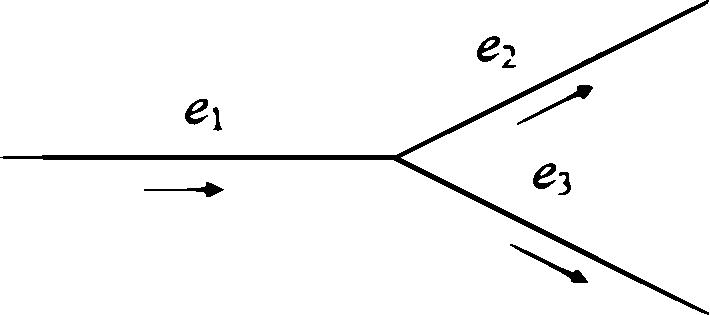
\includegraphics[width=0.5\linewidth]{StarGraph.pdf} % Raster format
%\includegraphics[width=0.7\linewidth]{figure.png} % Vector and raster format
%
% Vector drawings can be drawn in Inkscape editor
% https://inkscape.org/ru/download/
% The usual format of the editor is SVG, so the drawings must be exported in
% PDF or PNG (with a resolution of minimum 150 dpi, and maximum of 300 dpi).
%  \begin{center}    \missingfigure[figwidth=0.7\linewidth] \end{center}
  \caption{The metric star graph}\label{pic1}
\end{figure}

Now we define the vertex boundary conditions at the branched point
of the star graph, therefore we derive these boundary conditions
from conservation laws. One of the conservation laws is energy defined as

\begin{equation}
E = \sum_{j=1}^3 E_j,\label{conl1}
\end{equation}
where

\begin{equation}
E_j= \int _{e_j} \left[ \frac{1}{2} (\partial_t q_j)^2 +
\frac{1}{2} (\partial_x q_j)^2 - \frac{1}{2} q_j^2 + \frac{b_j}{4}
q_j^4 \right] dx.\label{energy1}
\end{equation}

From $\dot{E}=0$ we can get the following nonlinear boundary
condition as

\begin{equation}
\partial_x q_1 \partial_t q_1 |_{x=0} = \partial_x q_2 \partial_t q_2 |_{x=0} + \partial_x q_3 \partial_t q_3|_{x=0}.\label{nbc1}
\end{equation}

We need two types of boundary conditions to find a solution of
(\ref{kgeq1}) and to fulfil the nonlinear vertex boundary
condition (\ref{nbc1}). Therefore the first type of vertex
boundary conditions is the following weight continuity

\begin{equation}
 \alpha_1 q_1 |_{x=0}= \alpha_2 q_2 |_{x=0} = \alpha_3 q_3 |_{x=0},\label{wc1}
\end{equation}
the second type of vertex boundary conditions is given derivatives of wave functions at the branched point as Kirchhoff rule

\begin{equation}
 \frac{1}{\alpha_1} \partial_x q_1 |_{x=0} = \frac{1}{\alpha_2} \partial_x q_2 |_{x=0} + \frac{1}{\alpha_3} \partial_x q_3 |_{x=0}.\label{kr1}
\end{equation}

\section{The kink soliton solution of Klain-Gordon equation on the star graph with three edges}

The kink (antikink) soliton solution of Klein-Gordon equation
(\ref{kgeq1}) on the each bond $e_j$ of the metric star graph is
the following

\begin{equation}
 q_j (x,t) = \mp \frac{1}{\sqrt{b_j}} \, {\rm tanh} \left( \frac{x - l - \upsilon t}
{\sqrt{2(1 - \upsilon^2) }} \right),\label{sol1}
\end{equation}
where $l$ is the initial center of mass of soliton (the kink and
antikink soliton solutions are with the signs $-$ and $+$,
respectively). Fulfilling the vertex boundary conditions
(\ref{wc1})-(\ref{kr1}) we can get the following constrains

\begin{eqnarray}
\frac {\alpha_1}{\sqrt{b_1}} = \frac {\alpha_2}{\sqrt{b_2}} =
\frac{\alpha_3}{\sqrt{b_3}},\label{const1}\\
\frac {1}{\alpha_1 \sqrt{b_1}} = \frac {1}{\alpha_2 \sqrt{b_2}} +
\frac{1}{\alpha_3 \sqrt{b_3}}.\label{const2}
\end{eqnarray}

From Eq.s(\ref{const1}) and (\ref{const2}) we obtain the following sum rule for nonlinearities

\begin{equation}
\frac {1}{b_1} = \frac {1}{b_2} + \frac {1}{b_3}.\label{sr1}
\end{equation}


Using the kink (antikink) soliton solution of Klein-Gordon
equation (\ref{kgeq1}) with the sum rule for the nonlinearities
(\ref{sr1}) we can also show that the momentum is conserved.

\section{Conclusion}

In this work we studied the nonlinear Klein-Gordon equation on
the simplest metric graphs as the star graph with three
semi-infinite bonds. From the weight continuity and the condition for derivatives of the wave function as Kirchhoff rule we obtained nonlinear boundary conditions at the vertex (branched point) derived from the energy conservation law. We obtained the soliton solution on the metric star graph and the constrain as inverses of nonlinearities for the reflectionless transmission. We can also extend obtained results to other topologies such as tree and loop graphs.


% At the end of the text, acknowledgments are expressed, if you haven't
% made a footnote from the title. For example, we can write

\begin{thebibliography}{9} % or {99}, if there is more than ten references.

\bibitem{Book1} Ablowitz M.J., Segur H. Solitons and the Inverse Scattering Transform. Philadelphia, 1981.

\bibitem{Book2} Ablowitz M.J., Clarkson P.A. Solitons, Nonlinear Evolution Equations and Inverse Scattering. London, Cambridge University Press, 1991.

\bibitem{Proceedings1} Greiner W. Relativistic Quantum Mechanics-Wave Equations. Springer-Verlag, 3rd~ed. Berlin, 2000.

\bibitem{Article1} Ablowitz M.J., Kruskal M.D. and Ladik J.F. Solitary wave collisions. SIAM J. Appl. Math.~1979. Vol.~36, no~3. Pp.~428--437.

\bibitem{Article2} Jim´enez S., V´azquez L. Analysis of Four Numerical Schemes for a Nonlinear Klein-Gordon Equation. J. Appl. Math. 1990. Vol.35, Issue 1. Pp.~61--94.

\bibitem{Article22} Los Vu-Quos, Shaofan Li. Invariant-conserving finite difference algorithms for the nonlinear Klein-Gordon equation. J. Comp. Meth. in App. Mech. and Eng. (North-Holland, CMA 403), 1993. Vol. 107. Pp.~341--391.

\bibitem{Article3} Sabirov K.K., Babajanov D.B., Matrasulov D.U. and Kevrekidis P.G. Dynamics of dirac solitons in networks. J. Phys. A: Math. Theor.~2018. Vol.~51. P.~435203.

\bibitem{Article4} Sabirov K.K., Yusupov J.R., Matyokubov Kh.Sh., Susanto H., Matrasulov D.U. Networks with point-like nonlinearities. J. Nanosystems: Phys. Chem. Math.~2022. Vol.~13, no~1. P.~3035.

\bibitem{Article5} Yusupov J.R., Sabirov K.K., Asadov Q.U., Ehrhardt M., and Matrasulov D.U. Dirac particles in transparent quantum graphs: Tunable transport of relativistic quasiparticles in branched structures. J. Phys. Rev. E.~2020. Vol.~101. P.~062208.      
\end{thebibliography}
%\end{document}

%%% Local Variables:
%%% mode: latex
%%% TeX-master: t
%%% End:

\end{englisharticle}

\begin{englishtitle} % Настраивает LaTeX на использование английского языка
% Этот титульный лист верстается аналогично.
\title{Integration of the two-body problem equations using  polynomial total systems of PDEs}
% First author
\author{Levon~K.~Babadzanjanz   \and  Irina~Yu.~Pototskaya   \and  Yulia~Yu.~Pupysheva
}
\institute{St. Petersburg State University, St. Petersburg, Russia\\
  \email{j\_poupycheva@mail.ru}}
%  \and
%Affiliation, City, Country\\
%\email{email}}
% etc

\maketitle

\begin{abstract}
In this paper an original algorithm for solving the two-body problem using the Taylor method is presented. This method often has an advantage over other numerical integration methods in the accuracy of calculations. But the difficulty of its application lies in the need to repeatedly calculate the coefficients of Taylor series. Such calculations can make the method software implementation more cumbersome and slow. But when the integrated system has polynomial right-hand sides, the Taylor coefficients are calculated using a simple recurrent formula, and this numerical method becomes preferable for solving complex problems.
One of such tasks is the two-body problem. This is one of the most famous problems of classical mechanics. It consists in determining the motion of two material points interacting only with each other. Examples of this problem are the mutual motion of a planet and a satellite, a planet and a star, or an electron orbiting an atomic nucleus. The mathematical model of the two-body problem can be represented as a complete polynomial system of twenty-three partial differential equations. The solution of this system can be obtained by the Taylor series method. But, until recently, there was no literature describing an algorithm for such solving. Only in 2021, an article by the authors ``Estimates for Taylor series method to polynomial total systems of PDEs'' was published in the Bulletin of St. Petersburg State University, which provides the necessary mathematical tools for this.
In this paper the polynomial total system of partial differential equations constructed for the two-body problem is described. The algorithm for its numerical integration using the Taylor series method is presented. Recurrent formulas for Taylor coefficients obtained for the problem being solved are provided.


\keywords{two-body problem, Taylor Series Method, total polynomial PDE system, numerical PDE system integration} % в конце списка точка не ставится
\end{abstract}
\end{englishtitle}

\iffalse
\documentclass[12pt]{llncs}

% При использовании pdfLaTeX добавляется стандартный набор русификации babel.

\usepackage{iftex}

\ifPDFTeX
\usepackage[T2A]{fontenc}
\usepackage[utf8]{inputenc} % Кодировка utf-8, cp1251 и т.д.
\usepackage[english,russian]{babel}
\fi

\usepackage{todonotes}

\usepackage[russian]{nla}


\begin{document}
\fi

\title{Интегрирование уравнений задачи двух тел с помощью полной полиномиальной системы УрЧП}
% Первый автор
\author{Л.~К.~Бабаджанянц \and  И.~Ю.~Потоцкая  \and  Ю.~Ю.~Пупышева
} % обязательное поле

% Аффилиации пишутся в следующей форме, соединяя каждый институт при помощи \and.
\institute{Санкт-Петербургский государственный университет (СПбГУ), Санкт-Петербург, Россия\\
  \email{j\_poupycheva@mail.ru}
%  \and   % Разделяет институты и присваивает им номера по порядку.
%Институт (название в краткой форме), Город, Страна\\
%\email{email@examle.com}
% \and Другие авторы...
}

\maketitle

\begin{abstract}
В настоящей  работе представлен оригинальный алгоритм решения задачи двух тел с помощью метода рядов Тейлора.

\keywords{метод рядов Тейлора, задача двух тел, полная полиномиальная система УрЧП, коэффициенты Тейлора} % в конце списка точка не ставится
\end{abstract}

\section{Основные результаты} % не обязательное поле

Метод рядов Тейлора часто имеет преимущество перед другими численными методами интегрирования в точности вычислений. Но сложность его применения заключается в необходимости многократного вычисления коэффициентов рядов. В общем случае это может сделать программную реализацию метода более громоздкой и медленной. Но в случае, когда интегрируемая система имеет полиномиальные правые части, коэффициенты Тейлора вычисляются по простой рекуррентной формуле, и этот численный метод становится предпочтительнее для решения сложных задач.
Одной из таких задач является задача двух тел \cite{1975}, \cite{2007}.  Это одна из самых известных задач классической механики, которая заключается в том, чтобы определить движение двух материальных точек, взаимодействующих только друг с другом. Примерами такой задачи служат взаимное движение планеты и спутника, планеты и звезды или электрон, вращающийся вокруг атомного ядра. Математическая модель задачи двух тел может быть представлена в виде полной полиномиальной системы  из двадцати трёх уравнений в частных производных \cite{2016}, \cite{2020}. Решение такой системы может быть получено методом рядов Тейлора. Но, до недавнего времени, литературы, описывающей такой алгоритм для подобных систем, не было. Только в 2021 году в <<Вестнике СПбГУ>> была опубликована статья авторов <<Estimates for Taylor series method to polynomial total systems of PDEs>> \cite{2021}, дающая необходимые для этого математические инструменты.
В представленной работе описывается полная система полиномиальных уравнений в частных производных, построенная для задачи двух тел, излагается алгоритм её численного интегрирования методом рядов Тейлора, приводятся рекуррентные формулы для коэффициентов Тейлора, полученные для решаемой задачи.



\begin{thebibliography}{9} % или {99}, если ссылок больше десяти.



\bibitem{2021} Babadzanjanz~L.K., Pototskaya~I. Yu., Pupysheva~Yu. Yu. Estimates for
Taylor series method to polynomial total systems of PDEs~// Вестник Санкт-Петербургского
университета. Прикладная математика. Информатика. Процессы управления. 2021. Т. 17.
Вып. 1. С.~27–-39.

\bibitem{2020} Babadzanjanz~L.K., Pototskaya~I.Yu., Pupysheva~Yu.Yu. Estimates
for Taylor series method to linear total systems of PDEs // Вестник Санкт-Петербургского
университета. Прикладная математика. Информатика. Процессы управления. 2020. Т. 16.
Вып. 2. С.~112–-120

\bibitem{2016} Бабаджанянц~Л.К., Брэгман~А.М., Брэгман~К.М., Касикова~П.В., Петросян~Л.К. Вычисление проиводных по элементам для задачи двух тел // Технические науки -- от теории к практике: сб. ст. по матер. LXI междунар. науч.-практ. конф. № 8(56). Новосибирск: СибАК, 2016. С.~6--13.
    
\bibitem{1975} Дубошин~Г.Н. Небесная механика. Основные задачи и методы. 3-е изд. М.:~Наука, 1975.

\bibitem{2007} Холшевников~К.В., Титов~В.Б. Задача двух тел: Учеб. пособие. СПб: СПбГУ, 2007.


\end{thebibliography}

% После библиографического списка в русскоязычных статьях необходимо оформить
% англоязычный заголовок и аннотацию.




%\end{document} 


\begin{englisharticle}

\iffalse
\documentclass[12pt]{llncs}

\usepackage{todonotes}

\usepackage{nla} 

\begin{document}
\fi

\title{Existence and uniqueness of solutions to polyharmonic equations in weighted Sobolev spaces}

\author{Dzhamil Badardinov}
\institute{Novosibirsk State University, Novosibirsk, Russia\\
  \email{d.badardinov@g.nsu.ru}}
  
\maketitle

\begin{abstract}

The existence and uniqueness of solutions of an equation 
$$
\Delta^m\, u = f(x), \; x\in \mathbb{R}^n,
\eqno (1)
$$
are considered in the class of weighted Sobolev spaces \(W^{2m}_{p,\, \sigma}(\mathbb{R}^n)\).

\keywords{polyharmonic operator, weighted Sobolev spaces}
\end{abstract}

\section*{The main results} %optional section

\textsc{Definition.} A function \(u(x)\) belongs to weighted Sobolev space \(W^{2m}_{p,\, \sigma}(\mathbb{R}^n)\) if there exist generalized derivatives \(D^{\beta}_x u(x), \, |\beta| \leq 2m\) of \(u(x)\) in \(\mathbb{R}^n\), and
\[\left\|(1 + | x |)^{-\sigma(2m - |\beta|)} D_x^{\beta} u(x),\, L_p(\mathbb{R}^n)\right\| < \infty.\]

The norm in the space \(W^{2m}_{p,\, \sigma}(\mathbb{R}^n)\) is defined as
\[\left\|u(x),\,W^{2m}_{p,\sigma}(\mathbb{R}^n)\right\| = \sum\limits_{0 \leq |\beta| \leq 2m}
\left\|(1 + | x |)^{-\sigma(2m - |\beta|)} D_x^{\beta} u(x),\, L_p(\mathbb{R}^n)\right\|.\]

The following results are established.

\textbf{Theorem 1.}
\textsl{If \(\sigma > \frac{n}{2mp}\), \(j \leq 2m - 1 ,\; \frac{n}{2mp} + \frac{j}{2m} < \sigma \leq 1, \;\)
or
\(\;\sigma \geq 1,\, \sigma > \frac{n}{(2m-j)p},\) then the solution is defined up to a polynomial \(P_j(x)\) of degree not greater than j. 
}

\textbf{Theorem 2.} 
\textsl{If \(n>2m,\, \sigma = \frac{n}{2mp}\), then \(\forall\, f(x) \in L_p(\mathbb{R}^n),\) supp f is compact, \(\exists!\, u(x) \in W^{2m}_{p,\,\sigma}(\mathbb{R}^n)\) -- a solution of the equation (1), and the estimate takes place:
\[
\left\|u(x),\, W^{2m}_{p, \,\sigma}(\mathbb{R}^n)\right\|
\leq c\left\|f(x), L_p(\mathbb{R}^n)\right\|,
\]
where \(c = c(supp\, f)\).}

\textbf{Theorem 3.}
\textsl{If \(n > 2m - (N+1),\; \sigma \in [0, 1-\frac{n}{2mp'}],\, N \geq 0\) -- a natural number, such that \(1-\frac{n}{2mp'} - \frac{N+1}{2m} < \sigma \leq 1- \frac{n}{2mp'} - \frac{N}{2m}\), then the conditions 
\[\int\limits_{\mathbb{R}^n}\, x^{\beta} f(x) \,dx = 0\; \scriptstyle \forall \beta:\; |\beta| \,\leq\, N,\]
 are necessary and sufficient for the existence of solutions \(u(x) \in W^{2m}_{p, \,\sigma}(\mathbb{R}^n)\) of the equation (1) \(\forall\, f(x) \in L_p(\mathbb{R}^n),\) supp f is compact; if the conditions are fulfilled, then there exist a unique solution of the equation (1) and the estimate takes place: 
 \[\left\| u(x),\, W^{2m}_{p, \,\sigma}(\mathbb{R}^n)\right\| \leq c \left\|f(x),\, L_p(\mathbb{R}^n) \right\|,\]
 where \(c = c\,(\,supp\; f).\)}

The research method is based on using the fundamental solution of the
quasielliptic operator \(L(D_x)\), which was derived from the construction of approximate solutions of the equation (1) based on the method of integral representation of functions $f(x) \in L_p(R^n)$ suggested by S.V.~ Uspenskii~[1].

Similar questions for quasielliptic operators have been considered
in the works~[2]--[5].

% At the end of the text, acknowledgments are expressed, if you haven't
% made a footnote from the title. For example, we can write

\begin{thebibliography}{9} % or {99}, if there is more than ten references.

\bibitem{Uspenskii1972} Uspenskii S.\,V. On representation of functions determined by a certain class of hypoelliptic operators. Trudy Mat. Inst. Steklov Akad. Nauk SSSR.~1972. Vol.~117. Pp.~292--299.

\bibitem{Demidenko1993} Demidenko G.\,V. Integral operators determined by quasielliptic equations. I.
Sibirsk. Mat. Zh.~1993. Vol.~34, no.~6, Pp.~52--67.

\bibitem{Demidenko1998} Demidenko G.\,V. On quasielliptic operators in $R^n$.
Sibirsk. Mat. Zh.~1998. Vol.~39, no.~5, Pp.~884--893.

\bibitem{McOwen1979} McOwen R.\,C. The behavior of the Laplacian on weighted Sobolev spaces.
Comm. Pure Appl. Math.~1979. Vol.~32, no~6 Pp.~783--795.

\bibitem{Hile G.} Hile G. N. Fundamental Solutions and Mapping Properties of Semielliptic Operators. 
Math. Nachrichten.~2006. Vol.~279, no~13-14. Pp.~1538--1572.

\end{thebibliography}

%\end{document}
\end{englisharticle}


%\pagebreak

\begin{englishtitle} % Настраивает LaTeX на использование английского языка
% Этот титульный лист верстается аналогично.
\title{On the positivity of the cauchy function and the fundamental solution of a linear autonomous differential equation of neutral type}
% First author
\author{Anton Balandin
%  \and
%  Name FamilyName2\inst{2}
%  \and
%  Name FamilyName3\inst{1}
}
\institute{Perm National Research Polytechnic University, Perm, Russia\\
  \email{balandin-anton@yandex.ru}
%  \and
%Affiliation, City, Country\\
%\email{email}
}
% etc

\maketitle

\begin{abstract}
A linear autonomous differential equation of neutral type is considered. The positivity of the fundamental solution and the Cauchy function of this equation is investigated, and two-sided exponential estimates for these functions are established.

\keywords{functional differential equation, neutral type equation, exponential stability,
fundamental solution, Cauchy function} % в конце списка точка не ставится
\end{abstract}
\end{englishtitle}


\iffalse
\documentclass[12pt]{llncs}

% При использовании pdfLaTeX добавляется стандартный набор русификации babel.

\usepackage{iftex}

\ifPDFTeX
\usepackage[T2A]{fontenc}
\usepackage[utf8]{inputenc} % Кодировка utf-8, cp1251 и т.д.
\usepackage[english,russian]{babel}
\fi

\usepackage{todonotes}

\usepackage[russian]{nla}



\begin{document}
\fi
% Текст оформляется в соответствии с классом article, используя дополнения
% AMS.
%

\title{О положительности функции Коши и фундаментального решения линейного автономного дифференциального уравнения нейтрального типа\thanks{Работа выполнена при поддержке Министерства науки и высшего образования Российской Федерации, проект \textnumero~FSNM-2023-0003.}}
% Первый автор
\author{А.~С.~Баландин % \inst ставит циферку над автором.
%  \and  % разделяет авторов, в тексте выглядит как запятая.
% Второй автор
%  И.~О.~Фамилия\inst{2}
%  \and
% Третий автор
%  И.~О.~Фамилия\inst{1}
} % обязательное поле

% Аффилиации пишутся в следующей форме, соединяя каждый институт при помощи \and.
\institute{Пермский национальный исследовательский политехнический университет (ПНИПУ), Пермь, Россия\\
  \email{balandin-anton@yandex.ru}
%  \and   % Разделяет институты и присваивает им номера по порядку.
%Институт (название в краткой форме), Город, Страна\\
%\email{email@examle.com}
% \and Другие авторы...
}

\maketitle

\begin{abstract}
В работе рассматривается линейное автономное дифференциальное уравнение нейтрального типа. Исследуется положительность фундаментального решения и функции Коши данного уравнения, а также устанавливаются двусторонние экспоненциальные оценки на указанные функции.


\keywords{функционально-дифференциальное уравнение, уравнение нейтрального типа, экспоненциальная устойчивость, %положительность,
фундаментальное решение, функция Коши} % в конце списка точка не ставится
\end{abstract}

%\section{Основные результаты} % не обязательное поле

Рассмотрим линейное автономное дифференциальное уравнение нейтрального типа
\begin{equation}
\label{1_bal}
\begin{aligned}
\dot x(t)-a\dot x(t-h)-bx(t)-cx(t-h)=f(t),\quad t\ge0,\\
x(\xi)=\varphi(\xi),\quad\dot x(\xi)=\psi(\xi),\quad\xi\in[-h,0),
\end{aligned}
\end{equation}
где $a\in\mathbb R_+$, $b\in\mathbb R$, $c\in\mathbb R_-$, $h>0$, функция $f$ локально суммируема.

Уравнение~\eqref{1_bal} возникает в различных прикладных задачах: динамика популяции клеток, движение плоских упругих плит с учетом трения, исследование дефектов с помощью ультразвука.
С другой стороны, уравнение~\eqref{1_bal} обладает большим разнообразием асимптотических свойств решений и поэтому интересно также с теоретической точки зрения.

Через $I$ обозначим тождественный оператор, через $S_h$~--- оператор сдвига, действующий в пространстве непрерывных (кусочно-непрерывных, суммируемых) функций по правилу:
\begin{equation*}
(S_hy)(t)=\left\{
\begin{aligned}
&y(t-h),\quad&\mbox{при }t\ge h,\\
&0,&\mbox{при }t<h.\\
\end{aligned}
\right.
\end{equation*}
Уравнение~\eqref{1_bal} можно переписать в виде
\begin{equation}
\label{eq_main_bal}
\dot x(t)-a(S_h\dot x)(t)=bx(t)+c(S_hx)(t)+\sigma(t),\quad t\in\mathbb R_+,
\end{equation}
где роль внешнего возмущения играет функция $\sigma\colon\mathbb R_+\to\mathbb R$, суммируемая на $[-1,0]$ и
определяемая по правилу:
\begin{equation*}
\sigma(t)=\left\{
\begin{aligned}
&a\psi(t)+c\varphi(t),\quad\mbox{при }t\in[-1,0),\\
&0,\quad\mbox{при }t\notin[-1,0).
\end{aligned}
\right.
\end{equation*}

Под {\it решением} уравнения~\eqref{eq_main_bal} будем понимать абсолютно непрерывную на каждом конечном отрезке функцию $x\colon\mathbb R_+\to\mathbb R$, удовлетворяющую~\eqref{eq_main_bal} почти всюду на $\mathbb R_+$.

Как известно (см. \cite[с. 84, теорема 1.1]{bib_amr_bal}, \cite{bib_BalMal2_bal}), уравнение~\eqref{eq_main_bal} с заданными начальными условиями $x(0)\in\mathbb R$ однозначно разрешимо и его решение представимо в виде
\begin{equation*}
%\label{eq_Cauchy_formula_bal}
x(t)=X(t)x(0)+\int_0^tY(t-s)\sigma(s)\,ds,
\end{equation*}
где $X\colon\mathbb R_+\to\mathbb R$ называется {\it фундаментальным решением}, а $Y\colon\mathbb R_+\to\mathbb R$~--- {\it функцией Коши} уравнения~\eqref{eq_main_bal}.
На отрицательной полуоси $X$, $Y$ доопределим нулём.

Функция $X$ определяется как решение однородного уравнения вида~\eqref{eq_main_bal},
дополненного начальным условием $x(0)=1$.

%\begin{theorem}[\cite{bib_BalMal2_bal}]
{\bf Теорема 1 \cite{bib_BalMal2_bal}.} $X(t)=(I-aS_h)Y(t)$.
%\end{theorem}

Определим
$$
g_X(\gamma) = \frac{-\gamma(1 - a{e^{\gamma}}) - b - c{e^{\gamma}}}{1-ae^{\gamma}},\quad g_Y(\gamma) =-\gamma(1 - a{e^{\gamma}}) - b - ce^{\gamma},\quad \gamma \in \mathbb{R}.
$$

%\begin{theorem}
{\bf Теорема 2.}
{\it
Если $c\le0$, а для характеристической функции при некотором вещественном $\zeta>0$ выполнены условия $g_X(\zeta)=0$, $g'_X(\zeta)<0$, то фундаментальное решение уравнения~\eqref{eq_main_bal} имеет двустороннюю оценку
\begin{equation}
\label{eq9_bal}
e^{-\zeta t}\le X(t)\le -\frac1{g'_X(\zeta)}e^{-\zeta t},\quad t\ge 0,
\end{equation}
и, кроме того, $\lim\limits_{t\to\infty}X(t)e^{\zeta t}=-1/{g'_X(\zeta)}$.
}
%\end{theorem}

Показатель экспоненты и постоянные 1 и $-1/{g'_X(-\zeta)}$ в~\eqref{eq9_bal} точные.

%\begin{theorem}
{\bf Теорема 3.}
{\it
Если $c\le0$, а для характеристической функции при некотором вещественном $\zeta>0$ выполнены условия $g_Y(\zeta)=0$, $g'_Y(\zeta)<0$, то функция Коши уравнения~\eqref{eq_main_bal} имеет двустороннюю оценку
\begin{equation}
\label{eq10_bal}
e^{-\zeta t}\le Y(t)\le -\frac1{g'_Y(\zeta)}e^{-\zeta t},\quad t\ge 0,
\end{equation}
и, кроме того, $\lim\limits_{t\to\infty}Y(t)e^{\zeta t}=-1/{g'_Y(\zeta)}$.
}
%\end{theorem}

Показатель экспоненты и постоянные 1 и $-1/{g'_Y(-\zeta)}$ в~\eqref{eq10_bal} точные.

% Рисунки и таблицы оформляются по стандарту класса article. Например,

%\begin{figure}[htb]
%  \centering
  % Поддерживаются два формата:
  %\includegraphics[width=0.7\linewidth]{figure.pdf} % Растровый формат
  %\includegraphics[width=0.7\linewidth]{figure.png} % Векторный и растровый формат
  %
  % Векторные рисунки можно рисовать в редакторе Inkscape
  % https://inkscape.org/ru/download/
  % Основной формат этого редактора - SVG, поэтому рисунки необходимо экспортировать в
  % PDF или PNG (с разрешением - минимум 150 dpi, максимум - 300dpi).
%  \begin{center}
%    \missingfigure[figwidth=0.7\linewidth]{Уберите меня из статьи!}
%  \end{center}
%  \caption{Заголовок рисунка}\label{fig:example}
%\end{figure}

% Современные издательства требуют использовать кавычки-елочки << >>.

% В конце текста можно выразить благодарности, если этого не было
% сделано в ссылке с заголовка статьи, например,
%Работа выполнена при поддержке Министерства науки и высшего образования Российской Федерации, проект \textnumero~FSNM-2023-0005.
%

% Список литературы оформляется подобно ГОСТ-2008.
% Примеры оформления находятся по этому адресу -
%     https://narfu.ru/agtu/www.agtu.ru/fad08f5ab5ca9486942a52596ba6582elit.html
%

\begin{thebibliography}{9} % или {99}, если ссылок больше десяти.
\bibitem{bib_amr_bal} Азбелев~Н.В., Максимов~В.П., Рахматуллина~Л.Ф. Введение в теорию функ\-ци\-о\-наль\-но-дифференциальных уравнений. М.:~Наука,~1991.

\bibitem{bib_BalMal2_bal} Баландин А.С., Малыгина В.В. Об экспоненциальной устойчивости линейных диф\-фе\-рен\-циально-разностных уравнениях нейтрального типа~// Изв. вузов. Матем. 2007. \textnumero~7. С.~17--27.
%{Gantmakher} Гантмахер~Ф.Р. Теория матриц. М.:~Наука,~1966.

%\bibitem{Kholl} Современные численные методы решения обыкновенных дифференциальных уравнений~/ Под~ред.~Дж.~Холл, Дж.~Уатт. М.:~Мир,~1979.

    %{Aleksandrov1} Александров~А.Ю. Об устойчивости сложных систем в критических случаях~// Автоматика и телемеханика. 2001. \textnumero~9. С.~3--13.
%\bibitem{Moreau1977} Moreau~J.-J. Evolution problem associated with a moving convex set in a Hilbert space~// J.~Differential~Eq. 1977. Vol.~26. Pp.~347--374.

%\bibitem{Semenov} Семенов~А.А. Замечание о вычислительной сложности известных предположительно односторонних функций~// Тр.~XII Байкальской междунар. конф. <<Методы оптимизации и их приложения>>. Иркутск, 2001. С.~142--146.

\end{thebibliography}

% После библиографического списка в русскоязычных статьях необходимо оформить
% англоязычный заголовок.




%\end{document}

\begin{englisharticle}

\iffalse
\documentclass[12pt]{llncs}

\usepackage{todonotes}

\usepackage{nla} 

\begin{document}
\fi

\title{Solvability of a problem with the integral gluing condition for a loaded integro-differential equation }

\author{Umida Baltaeva\inst{1} \and Yulduz Babajanova\inst{2} \and Boburjon Khasanov\inst{3}
}
\institute{Khorezm Mamun Academy, \\Khorezm, Uzbekistan\\
  \email{umida{\underline{ }}baltayeva@mail.ru}
  \and
Khorezm Mamun Academy, \\Khorezm, Uzbekistan\\
\email{yulduzb90@gmail.com}
 \and
Khorezm Mamun Academy, \\Khorezm, Uzbekistan\\
\email{xasanovboburjon.1993@gmail.com}}

\maketitle

\begin{abstract}
\keywords{Mixed type equation, parabolic-hyperbolic type, integral condition, Riemann-Liouville fractional integral operator}
\end{abstract}

Let $ D $ be a domain bounded by segments $ y = 0$, $x = 1$, $y = 1$
and $x = -1$. We introduce the following notations
$$D_{1}=D\cap\{x>0\},\,\ D_{2}=D\cap\{x<0\},\,\,I=\{ (x,y):x=0,
0<y<1\}.$$

We consider the following linear loaded [1],[2] integro-differential
equation


\begin{equation}
u_{xx} - {\frac{{1 - sgny}}{{2}}}u_{yy} - {\frac{{1 +
			sgny}}{{2}}}u_{y} + M u=0,\,\textrm{ in }\ D_{k},
\end{equation}
where $M u\equiv\sum\limits_{i=1}^{n}a_{i}(x,y)D_{0y}^{\alpha_{i}}
u(0,y)$ in $D_{1}$ and $M
u\equiv\sum\limits_{i=1}^{n}b_{i}(x,y)D_{0y}^{\beta_{i}}u(0,y)$ in
$D_{2}$, respectively, $D_{0y}^{\gamma }$ Riemann-Liouville
fractional integral operator of order
$\gamma\,(\gamma=\alpha_{i},\beta_{i})$.
 We assume that the functions  $a_{i}(x,y) and $  $ b_{i}(x,y)  (i=1,n) $ have a Holder continuous derivative on the closure of domain $\overline{D}$.

Consider the following mixed problem with integral gluing conditions
for a loaded integro-differential equation (1).

$\textbf{Problem 1.}$ Find a function $u(x,y)$ satisfying the
conditions:

1) $u(x,y)\in C (\bar{D_{k}})\cap C^{1}(D_{k}\cup I)$;

2) $u(x,y)$ is a regular solution of (1) in the domains $D_{k}(k=1,2)$;

3) the following gluing conditions
\begin{equation}
\left.\begin{aligned}
\tau_{1}(y)&=\mu(y)\tau_{2}(y)+\sigma(y),\\
\nu_{1}(y)&=\int\limits_{0}^{y}\gamma(y,\eta)\nu_{2}(\eta)d\eta+\delta(y)\nu_{2}(y)+\xi(y)\tau_{2}(y)+\theta(y),
\end{aligned} \right\}
\end{equation}
are satisfied on $I$, $ \tau_{1}(y)=u(+0,y),\,
\nu_{1}(y)=u_{x}(+0,y), $
$\tau_{2}(y)=u(-0,y),\,\nu_{2}(y)=u_{x}(-0,y); $

4) satisfies boundary conditions:
\begin{equation}
u(-1,y)=\varphi_{1}(y), \ \ \ u_{x}(1,y)=\varphi_{2}(y),\ \ \ 0\leq y\leq 1,
\end{equation}
\begin{equation}
u(x,0)=\psi_{1}(x), \ \ \ u_{y}(x,0)=0,\ \ \ -1\leq x\leq 0,
\end{equation}
\begin{equation}
u(x,0)=\psi_{2}(x),  \ \ \ 0\leq x\leq 1,
\end{equation}
where $ \varphi _1 (y),\varphi _2 (y),\psi _1 (x),\psi _2 (x),$ $
\mu(y),$ $ \sigma(y),$
$  \delta(y),$ $ \gamma_{y}(y,\eta),$ $  \xi(y),  \theta(y) $ are given
functions, $\mu(y)\neq 0,$ $ \gamma^{2}(y,\eta)+\delta^{2}(y)\neq 0, $ moreover,
\begin{equation*}
\varphi_{1}(0)=\psi_{1}(-1), \,\,  \varphi_{2}(0)=\psi'_{2}(1),\,\,
\psi_{2}(0)=\mu(0)\psi_{1}(0)+\sigma(0).
\end{equation*}

\begin{theorem}
If $\psi''_{1}(x),$ $  \varphi''_{1}(y),$ $  \psi''_{2}(x),$ $ \varphi_{2}(y),$ $  c_{1}(x,y),$  $  \mu'(y),$ $  \sigma'(y),$ $  \delta'(y),$ $ \gamma_{y}(y,\eta),$ $  \xi'(y),  \theta'(y) $ are Holder continuous and 
\begin{equation}\left.\begin{aligned}
\delta(0)\psi'_{1}(0)+\xi(0)\psi_{1}(0)+\theta(0)-\psi'_{2}(0)=0,\ \ \text{if} \ \ \delta(y)\neq 0,\\
\xi(0)\psi_{1}(0)+\theta(0)-\psi_{2}(0)=0,\ \ \sigma'(0)+\mu'(0)\psi_{1}(0)=0,\ \ \  \text{if}\ \ \ \delta(y)\equiv 0,\\	\varphi_{1}(0)=\psi_{1}(-1),\ \ \ \varphi_{2}(0)=0,
\end{aligned} \right\}
\end{equation}
	then there exists a unique solution to problem 1.
\end{theorem}

\begin{thebibliography}{9} % or {99}, if there is more than ten references.
\bibitem{ ANakhushev2012}Nakhushev A. M. Loaded Equations and Their Application, Moscow, Nauka, 2012.~[In Russian]
\bibitem{Baltaeva2021}Baltaeva U.I. Alikulov Y., Baltaeva I.I., Ashirova A. Analog of
the Darboux problem for a loaded integro-differential equation involving the Caputo fractional derivative.  Nanosystems physics, chemistry, mathematics.~2021. Vol.~4. Pp.~418--424.
\end{thebibliography}
%\end{document}

\end{englisharticle}

\begin{englishtitle} % Настраивает LaTeX на использование английского языка
% Этот титульный лист верстается аналогично.
\title{One problem of achieving an incompletely known target set}
% First author
\author{Alexandr Barinov} 

\institute{Chelyabinsk State University, Chelyabinsk,Russia\\
  \email{barinovalexmih@mail.ru}}
 % \and
%Affiliation, City, Country\\
%\email{email@example.com}}
% etc

\maketitle

\begin{abstract}
We consider the problem of passing a maze with exits unknown in advance, namely, in the maze there are $2$ exits, one of which is real and the other false. Which of the outputs is real at the initial moment of time is unknown. Subsequently, at each step, with probability $p$, the position of the real exit is revealed, so the goal of the decision maker is to move along a trajectory from which he can get to any exit as long as possible.

\keywords{optimal control, finding a path in a maze, Lee algorithm} % в конце списка точка не ставится
\end{abstract}
\end{englishtitle}

\iffalse
%%%%%%%%%%%%%%%%%%%%%%%%%%%%%%%%%%%%%%%%%%%%%%%%%%%%%%%%%%%%%%%%%%%%%%%%
%
%  This is the template file for the 6th International conference
%  NONLINEAR ANALYSIS AND EXTREMAL PROBLEMS
%  June 25-30, 2018
%  Irkutsk, Russia
%
%%%%%%%%%%%%%%%%%%%%%%%%%%%%%%%%%%%%%%%%%%%%%%%%%%%%%%%%%%%%%%%%%%%%%%%%


\documentclass[12pt]{llncs}  

% При использовании pdfLaTeX добавляется стандартный набор русификации babel.

\usepackage{iftex}

\ifPDFTeX
\usepackage[T2A]{fontenc}
\usepackage[utf8]{inputenc} % Кодировка utf-8, cp1251 и т.д.
\usepackage[english,russian]{babel}
\fi

\usepackage{todonotes} 

\usepackage[russian]{nla}

\begin{document}
\fi

\title{Одна задача достижения не полностью известного целевого множества}%\thanks{Работа выполнена при поддержке РФФИ (РНФ, другие фонды), проект \textnumero~00-00-00000.}}
% Первый автор
\author{А.~М.~Баринов
}

% Аффилиации пишутся в следующей форме, соединяя каждый институт при помощи \and.
\institute{Челябинский государственный университет (ФГБОУ ВО <<ЧелГУ>>), Челябинск, Россия \\
  \email{barinovalexmih@mail.ru}
 % \and   % Разделяет институты и присваивает им номера по порядку.
%Институт (название в краткой форме), Город, Страна\\
  %\email{email@example.com}
% \and Другие авторы...
}

\maketitle

\begin{abstract}
Рассматривается задача о прохождении лабиринта с неизвестными заранее выходами, а именно в лабиринте имеется $2$ выхода, один из которых настоящий, а другой ложный. Какой из выходов настоящий в начальный момент времени неизвестно. В дальнейшем, на каждом шагу с вероятностью $p$ открывается положение настоящего выхода, поэтому цель ЛПР ---  движение по траектории, из которой он как можно дольше может попасть в любой выход.

\keywords{оптимальное управление, поиск пути в лабиринте, алгоритм Ли } % в конце списка точка не ставится
\end{abstract}

%\section{Основные результаты} % не обязательное поле

Задачи нахождения алгоритмов выбора пути в условиях неопределенности исследовались во многих рабодах, например\cite{bar1,bar2}. В докладе рассматривается следующая задача.\\

Пусть позиция $x$ задается вектор-столбцом $x=(x_1,x_2)'$ где $x_1\in \{1,2,\ldots,n\},$ $x_2\in \{1,2,\ldots,m\}$, штрих означает операцию  транспонирования.

Множество всех позиций задачи обозначим
\begin{center}
 $X=\{x=(x_1,x_2)' || x_1, x_2\in \mathbb{N}, x_1\leq n, x_2\leq m\}$,
\end{center}
а множество допустимых позиций $P \subseteq X$.

Рассматривается задача с дискретным временем $t$, где $t\in\{0,1,2,\ldots,T\}$.
Положение системы в момент времени $t+1$  $(t \in 0, \ldots,T-1)$ задается системой разностных уравнений
\begin{equation} \label{eq1}
		\begin{cases}% создание окружения для систем уравнений
			x_1(t+1)=x_1(t)+u_1(t),\\
			x_2(t+1)=x_2(t)+u_2(t),\\
		\end{cases}
\end{equation}
где управление $u(t)$ в момент времени $t$ имеет вид
\begin{equation} \label{eq2}
u(t)= (u_1(t),u_2(t))', \;\;\;\; u_i(t) \in \{-1,0, 1\} \;\; (i=1,2).
\end{equation}

Система (1), (2) описывает перемещение точки, расположенной в клетке прямоугольной сетки в одну из восьми соседних клеток, либо отсутствие перемещения (см. рис.\ref{fig1}).
\begin{figure}[h]
\centering
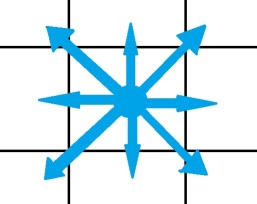
\includegraphics[width=0.4\linewidth]{ris.jpg}
\caption{Направления перемещения}
\label{fig1}
\end{figure}
Такая система, с учетом множества допустимых позиций, может трактоваться как движение точки по лабиринту.

Задано начальное положение системы
\begin{equation} \label{eq3}
 x(0)=(x_1(0),x_2(0))'=x^0=(x_1^0,x_2^0)'.
\end{equation}

Предполагается, что cистема в момент времени $T$ должна попасть в целевую позицию (выход из лабиринта), о которой известно, что это либо $x^*$, либо $x^{**}$ (то есть должно быть выполнено одно из условий $x(T)=x^*$, или $x(T)=x^{**}$, но какое -- заранее неизвестно.

На каждом шаге с вероятностью $p$ становится известно настоящее положение выхода.

Пусть момент времени $T_1<T$ --- это последний момент времени, в который ЛПР, двигаясь по некоторой траектории, может привести систему как в положение $x(T)=x^*$, так и в $x(T)=x^{**}$.

Вероятность того, что ЛПР откроется положение настоящего выхода к моменту времени $T_1$ будет 
\begin{center}
$P_{T_1}=p+(1-p)p+{(1-p)^2}p+\ldots+{(1-p)^{{T_1}-1}p}$.
\end{center}
Перед ЛПР стоит следующая задача
\begin{center}
$P=P_{T_1}+\frac{1-P_{T_1}}{2}\rightarrow max$,
\end{center}
что равносильно 
\begin{equation} \label{eq4}
T_1 \rightarrow max .
\end{equation}


Решением задачи оптимального управления (1)--(4) будем называть пару $(\hat{u}, \hat{x}(\cdot))$, где
оптимальное управление
$$
\hat{u}=(\hat{u}(0),\ldots ,\hat{u}({{T}_{1}}-1),({{{\hat{u}}}^{*}}({{T}_{1}}),{{{\hat{u}}}^{*}}({{T}_{1}})),\ldots ,({{{\hat{u}}}^{*}}(T-1),{{{\hat{u}}}^{**}}(T-1))),
$$
а, определяемая этим управлением, оптимальная траектория
$$
\hat{x}(\cdot)=(\hat{x}(0),\ldots ,\hat{x}({{T}_{1}}),({{{\hat{x}}}^{*}}({{T}_{1}}+1),{{{\hat{x}}}^{**}}({{T}_{1}}+1)),\ldots ,({{{\hat{x}}}^{*}}(T),{{{\hat{x}}}^{*}}(T))).
$$

В докладе предлагается алгоритм решения задачи (1)--(4) и приводятся результаты численного моделирования.


\setcounter{equation}{0}
\setcounter{figure}{0}

\small


\begin{thebibliography}{9} % или {99}, если ссылок больше десяти.
\bibitem{bar1} Кирильченко А.А. Обоснование алгоритмов выбора пути в условиях неопределенности  // Препринт Ин-та прикл. матем. им. М.В. Келдыша АН СССР, 1991, \textnumero~108, 25~с.

\bibitem{bar2} Бакиров А. К., Кирильченко А. А. Исследование особых ситуаций для задачи выбора пути в условиях неопределенности // Препринты ИПМ им. МВ Келдыша.  2001.   \textnumero~31.

\end{thebibliography}

% После библиографического списка в русскоязычных статьях необходимо оформить
% англоязычный заголовок.




%\end{document}



\begin{englishtitle} % Настраивает LaTeX на использование английского языка
% Этот титульный лист верстается аналогично.
\title{Study of the solvability of quasi-parabolic degenerate integro-differential equations of Volterra type}
% First author
\author{B.~Kh.~Barotov\inst{1}   \and  A.~I.~Kozhanov\inst{1,2}
}
\institute{Novosibirsk State University, Novosibirsk, Russia\\
  \email{b.barotov@g.nsu.ru}
  \and
Sobolev Institute of Mathematics, Novosibirsk, Russia\\
\email{kozhanov@math.nsc.ru}}
% etc

\maketitle

\begin{abstract}
The report presents results on the solvability of boundary value problems for quasi-parabolic integro-differential equations

$$ h(t)u_{ttt}(x,t)+ Au(x,t) +\int\limits_0^t R(t-\tau) (Bu)(x,\tau)d\tau =f(x,t),  $$

in which the function $h(t)$ can vanish, $A$ and $B$ are either identical operators or linear operators elliptic in spatial variables.  For the problems under study, the existence and uniqueness theorems for regular solutions are obtained, that is, solutions that have all derivatives generalized according to S.L. Sobolev and included in the corresponding equation.

\keywords{quasi-parabolic, integro-differential equations of Volterra type, degeneration, boundary value problems, regular solutions, existence, uniqueness } % в конце списка точка не ставится
\end{abstract}
\end{englishtitle}


\iffalse
%%%%%%%%%%%%%%%%%%%%%%%%%%%%%%%%%%%%%%%%%%%%%%%%%%%%%%%%%%%%%%%%%%%%%%%%
%
%  This is the template file for the 6th International conference
%  NONLINEAR ANALYSIS AND EXTREMAL PROBLEMS
%  June 25-30, 2018
%  Irkutsk, Russia
%
%%%%%%%%%%%%%%%%%%%%%%%%%%%%%%%%%%%%%%%%%%%%%%%%%%%%%%%%%%%%%%%%%%%%%%%%


\documentclass[12pt]{llncs}  

% При использовании pdfLaTeX добавляется стандартный набор русификации babel.

\usepackage{iftex}

\ifPDFTeX
\usepackage[T2A]{fontenc}
\usepackage[utf8]{inputenc} % Кодировка utf-8, cp1251 и т.д.
\usepackage[english,russian]{babel}
\fi

\usepackage{todonotes} 

\usepackage[russian]{nla}

\begin{document}
\fi

\title{Исследование разрешимости квазипараболических вырождающихся интегро-дифференциальных уравнений вольтерровского типа}
% Первый автор
\author{Б.~Х.~Баротов\inst{1}  \and А.~И.~Кожанов\inst{1,2}
}

% Аффилиации пишутся в следующей форме, соединяя каждый институт при помощи \and.
\institute{Новосибирский государственный университет, Новосибирск, Россия \\
  \email{ b.barotov@g.nsu.ru}
  \and   % Разделяет институты и присваивает им номера по порядку.
Институт математики им. С.Л. Соболева СО РАН, Новосибирск, Россия\\
  \email{kozhanov@math.nsc.ru}
% \and Другие авторы...
}

\maketitle

\begin{abstract}
В докладе излагаются результаты о разрешимости краевых задач для квазипараболических интегро-дифференциальных  уравнений 

	
 $$ h(t)u_{ttt}(x,t)+ Au(x,t) +\int\limits_0^t R(t-\tau) (Bu)(x,\tau)d\tau =f(x,t),  $$
 в которых  функция $h(t)$ может обращаться  в нуль, $A$ и $B$ есть  либо  тождественные  операторы, либо  линейные эллиптические по пространственным  переменным операторы. Для изучаемых задач получены теоремы существования и единственности регулярных решений-то есть решений, имеющих все обобщенные по С.Л. Соболеву производные, входящие в соответствующее уравнение.

\keywords{квазипараболические, интегро-дифференциальные уравнения вольтерровского типа, вырождение, краевые задачи, регулярные решениях, существование, единственность} % в конце списка точка не ставится
\end{abstract}








% После библиографического списка в русскоязычных статьях необходимо оформить
% англоязычный заголовок.



%\end{document}



\begin{englishtitle} % Настраивает LaTeX на использование английского языка  % проверочное исправление
% Этот титульный лист верстается аналогично.
\title{Realization of additional variables method in problems of dynamics}
% First author
\author{Mikhail Bekhovskiy}
\institute{Saint-Petersburg State University, Saint-Petersburg, Russia\\
  \email{mbexovskij@gmail.com}}
% etc

\maketitle

\begin{abstract}
We propose adapted algorithms based on additional variables method \cite{AlgoDE, AlgoFunc, AVM} and their program realization in Python. Using our program one can reduce systems of total partial differential equations to a form with polynomial right-hand sides (which in turn can be numerically solved by efficient special methods, for example \cite{TSM}) or symbolically differentiate multivariable functions. The program can transform expressions written in terms of library of functions and basic arithmetical operators. The library is organized as a separate module within the program which can be modified by a potential user. This allows our program to be used to symbolically differentiate multivariable functions written in terms of special functions not represented in popular computer algebra systems. Additionally we could not find an existing program, module or library with which one could automatically reduce systems of differential equations to polynomial form.
Our program is located in a public repository on GitHub\cite{repo} and does not have any proprietary dependencies.
The work of our program is demonstrated on some model examples.

\keywords{symbolic differentiation, polynomial system, additional variables method} % в конце списка точка не ставится
\end{abstract}
\end{englishtitle}

\iffalse
%%%%%%%%%%%%%%%%%%%%%%%%%%%%%%%%%%%%%%%%%%%%%%%%%%%%%%%%%%%%%%%%%%%%%%%%
%
%  This is the template file for the 6th International conference
%  NONLINEAR ANALYSIS AND EXTREMAL PROBLEMS
%  June 25-30, 2018
%  Irkutsk, Russia
%
%%%%%%%%%%%%%%%%%%%%%%%%%%%%%%%%%%%%%%%%%%%%%%%%%%%%%%%%%%%%%%%%%%%%%%%%


\documentclass[12pt]{llncs}  

% При использовании pdfLaTeX добавляется стандартный набор русификации babel.

\usepackage{iftex}

\ifPDFTeX
\usepackage[T2A]{fontenc}
\usepackage[utf8]{inputenc} % Кодировка utf-8, cp1251 и т.д.
\usepackage[english,russian]{babel}
\fi

\usepackage{todonotes} 

\usepackage[russian]{nla}

\begin{document}
\fi

\title{Реализация метода дополнительных переменных в задачах динамики}
% Первый автор
\author{М.~А.~Беховский}

% Аффилиации пишутся в следующей форме, соединяя каждый институт при помощи \and.
\institute{СПбГУ, Санкт-Петербург, Российская Федерация \\
  \email{mbexovskij@gmail.com}
}

\maketitle

\begin{abstract}
Предлагаются адаптированные алгоритмы и программная реализация метода дополнительных переменных \cite{AlgoDE, AlgoFunc, AVM} на языке Python. Метод позволяет сводить полные системы дифференциальных уравнений в частных производных первого порядка к эквивалентным системам с полиномиальными правыми частями. Численное решение полученных систем, в свою очередь, можно осуществлять предназначенными для полиномиальных систем методами, более эффективными, чем численные методы решения дифференциальных уравнений общего назначения\cite{TSM}. Кроме того, представленные алгоритмы позволяют осуществлять символьное дифференцирование функций многих переменных широкого класса \cite{AVM}.
Помимо самих алгоритмов \cite{AlgoDE, AlgoFunc}, адаптированных для реализации на языке Python, ключевой составляющей программы является библиотека функций.  В терминах представленной библиотеки могут быть записаны обрабатываемые выражения. Достоинством явного выделения указанной библиотеки является возможность, без особых затруднений, пополнять ее нужными пользователю функциями. Благодаря этому после незначительной модификации пользователь сможет использовать нашу программу для работы с выражениями, содержащими функции, отсутствующие в поставляемой с программой версией библиотеки. При использовании предлагаемой программы для символьного дифференцирования данное свойство, как нам кажется, положительно выделяет ее на фоне популярных пакетов символьной алгебры. Изменение ядра существующих пакетов либо невозможно (в случае коммерческого ПО с закрытым исходным кодом такого, как: Mathematica, Matlab, Maple), либо связано со значительными трудностями из-за ориентирования пакета на решение широкого круга разнородных задач (например, пакет SymPy). В то же время методы, позволяющие сводить системы уравнений к полиномиальной форме, не были нами обнаружены в указанных выше пакетах. 
Данная программа расположена в публичном репозитории\cite{repo} вместе с руководством к использованию и не имеет проприетарных зависимостей (распространяется в качестве свободного программного обеспечения с открытым исходным кодом), что позволяет всякому желающему использовать ее в своей работе без дополнительных издержек.
Корректность и актуальность нашей программы демонстрируется на модельных примерах.

\keywords{символьное дифференцирование, полиномиальная система, метод дополнительных переменных} % в конце списка точка не ставится
\end{abstract}

\begin{thebibliography}{9} % или {99}, если ссылок больше десяти.

\bibitem{AlgoDE} Бабаджанянц~Л.К., Брэгман~К.М. Алгоритм метода дополнительных переменных~// Вестник СПбГУ. Сер. 10. 2012. \textnumero~2. С.~3--12.

\bibitem{AlgoFunc} Брэгман~К.М. Алгоритм дифференцирования, основанный на методе дополнительных переменных~// Вестник СПбГУ. Сер. 10. 2013. \textnumero~2. С.~14--24.

\bibitem{AVM} Бабаджанянц~Л.К. Метод дополнительных переменных~// Вестник СПбГУ. Сер.10. 2010. \textnumero~1. С.~3--11.

\bibitem{TSM} Бабаджанянц~Л.К. Большаков А.И. Реализация метода рядов Тейлора для решения обыкновенных дифференциальных уравнений~// Вычислительные методы и программирование. Науч.-исслед. вычисл. центр Моск. ун-та им. М.В. Ломоносова. 2012. Т.~13. С.~497--510.

\bibitem{repo} AVM program GitHub repository~// URL: https://github.com/MikhailBekhovskiy/AVM
\end{thebibliography}

% После библиографического списка в русскоязычных статьях необходимо оформить
% англоязычный заголовок.




%\end{document}



\begin{englishtitle} % Настраивает LaTeX на использование английского языка
% Этот титульный лист верстается аналогично.
\title{Dualism of theories of solitonic solutions of infinite-dimensional dynamic systems and functional- differential equations of pointwise type}
% First author
\author{Levon Beklaryan\inst{1} \and  Armen Beklaryan\inst{2}
}
\institute{Central Economics and Mathematics Institute of Russian Academy of Sciences, Moscow, Russia\\
  \email{lbeklaryan@outlook.com}
  \and
HSE University, Moscow, Russia\\
\email{abeklaryan@hse.ru}}
% etc

\maketitle

\begin{abstract}
The formalism which central element is existence of one-to-one correcpondence  between solitonic solutions of an infinite-dimensional dynamic system and solutions of the induced functional-differential equation of pointwise type is presented. Within such approach the task about longitudinal fluctuations of the infinite absolutely elastic rod described  by finite  difference analog of the wave equation is studied. For such system the family of bounded solitonic solutions is described. 

\keywords{solitonic solutions, functional-differential equations, wave equation} % в конце списка точка не ставится
\end{abstract}
\end{englishtitle}

\iffalse
\documentclass[12pt]{llncs} 
\usepackage{amsfonts,amsmath,array}
\usepackage{amssymb}


\usepackage{iftex}

\ifPDFTeX
\usepackage[T2A]{fontenc}
\usepackage[utf8]{inputenc} % Кодировка utf-8, cp1251 и т.д.
\usepackage[english,russian]{babel}
\fi

\usepackage{todonotes} 

\usepackage[russian]{nla}

\begin{document}
\fi

\title{Дуализм теорий  солитонных решений бесконечномерных динамических систем и функционально-дифференциальных уравнений точечного типа\thanks{Исследование выполнено за счет гранта Российского научного фонда (проект \textnumero~23-11-00080)}}
% Первый автор
\author{Л.~А.~Бекларян\inst{1} \and А.~Л.~Бекларян\inst{2}
}

% Аффилиации пишутся в следующей форме, соединяя каждый институт при помощи \and.
\institute{Центральный Экономико-Математический Институт РАН, Москва, Россия \\
  \email{lbeklaryan@outlook.com}
  \and   % Разделяет институты и присваивает им номера по порядку.
Национальный исследовательский университет Высшая школа экономики, Москва, Россия\\
  \email{abeklaryan@hse.ru}
% \and Другие авторы...
}

\maketitle

\begin{abstract}
 Представлен  формализм, центральным элементом которого является существование взаимно однозначного соответствия между солитонными решениями бесконечномерной динамической системы  и решениями индуцированного функцио\-наль\-но-дифференциального уравнения точечного типа. В рамках такого подхода изучена задача о продольных колебаниях бесконечного абсолютно упругого стержня, описываемого конечно разностным аналогом волнового уравнения. Для такой системы описано семейство ограниченных солитонных решений.

\keywords{солитонные решения, функционально-дифференциальные уравнения, волновое уравнение} % в конце списка точка не ставится
\end{abstract}

\section{Основные результаты} % не обязательное поле

Совокупность конструкций $\big(\Upsilon,d,s,\eta,G_\Gamma|Q,g\big)$ называется {\it солитонным букетом} и однозначно определяется набором $\Gamma=(\Upsilon,d,s,\eta,Q,g)$, где:
\begin{itemize}
\item[(1)] конечно порожденная группа $\Upsilon$ с образующими $\{\check{\gamma_1},\ldots,\check{\gamma_d}\}$ и выделенными элементами $\{\gamma_1,\ldots,\gamma_s\}$, а также соответствующее пространство $\mathcal K^n_\Upsilon=\overline{\prod}_{\gamma\in \Gamma} R^n_\gamma$, $R^n_\gamma=\mathbb R^n$ бесконечных последовательностей $\varkappa=\{x_\gamma\}_{\gamma\in \Gamma}$, $x_\gamma\in \mathbb R^n$, $x_\gamma=(x_\gamma^1,\ldots, x_\gamma^n)^{'}$ со стандартной топологией полного прямого произведения;
\item[(2)] конечно порожденная группа сдвигов $\mathbb T_\Upsilon=\{T_\gamma: \gamma \in \Upsilon\}$, действующая в пространстве $\mathcal K^n_\Upsilon$ по следующему правилу
    $$
    T_{\bar{\gamma}}\{x_\gamma\}_{\gamma \in \Upsilon }=\{x_{\gamma\bar{\gamma}}\}_{\gamma \in \Upsilon},\quad \bar{\gamma}\in \Upsilon,\quad \{x_\gamma\}_{\gamma \in \Upsilon }\in \mathcal K^n_\Upsilon,\quad T_{\bar{\gamma}} \in \mathbb T_\Upsilon;
    $$
\item[(3)] эпиморфизм $\eta: \Upsilon \rightarrow Q$, где $Q$ группа диффеоморфизмов прямой, сохраняющих ориентацию, и, соответственно, $Q$ конечно порожденная группа с образующими $\check{q_j}=\eta(\check{\gamma_j})$, $j=1,\ldots,d$ и выделенными элементами $q_j=\eta({\gamma_j})$, $j=1,\ldots,s$;
\item[(4)] функция $g:\mathbb R\times \mathbb R^{ns} \rightarrow \mathbb R^{n}$ измеримая по $t\in \mathbb R$ при каждом $x_1,\ldots,x_s\in \mathbb R$ и при почти каждом $t\in \mathbb R$ непрерывная по $x_1,\ldots,x_s\in \mathbb R^n$ (условия Каратеодори);
\item[(5)] оператор
$$
G_{\Gamma}: \mathbb R\times \mathcal K^n_\Upsilon \rightarrow \mathcal K^n_\Upsilon,\quad \Gamma=(\Upsilon,d,s,\eta,Q,g)
$$
такой, что координата $\big(G_{\Gamma}(t,\varkappa)\big)_e$ бесконечномерной вектор-функции $G_{\Gamma}(t,\varkappa)$, соответствующая единичному элементу $e$ группы $\Upsilon$, зависит только лишь от конечного числа координат и равна
$$
\big(G_{\Gamma}(t,\varkappa)\big)_e=g\big(t,x_{{\gamma}_1},\ldots,x_{{\gamma}_s}\big);
$$
\item[(6)] при почти каждом $t \in \mathbb R $ выполняются ``почти перестановочные'' соотношения
$$
T_{\bar\gamma} G_{\Gamma}(t,\varkappa)=\frac{d}{dt}\eta(\bar\gamma)(t)\cdot G_{\Gamma}(\eta(\bar\gamma)(t),T_{\bar\gamma}\varkappa), \forall \varkappa \in \mathcal  K^n_\Upsilon, \forall \bar\gamma\in \Upsilon.
$$
\end{itemize}

Для солитонного букета $\big(\Upsilon,d,s,\eta,G_\Gamma| Q,g\big)$ с $\Gamma=(\Upsilon,d,s,\eta,Q,g)$ в фазовом пространстве ${\mathcal K}^n_\Upsilon$ с фазовой переменной $\varkappa\in{\mathcal K}^n_\Upsilon$ определим систему
$$
\dot{\varkappa}(t)=G_\Gamma(t,\varkappa),\quad  \text{для п.в. } t\in \mathbb R,\eqno{(1)}
$$
$$
\varkappa(\eta(\bar{\gamma})(t))=T_{\bar{\gamma}}\varkappa(t),\quad \forall t\in \mathbb R, \quad \forall\bar{\gamma}\in \Upsilon,\eqno{(2)}
$$
где производная в бесконечномерном ОДУ (1) понимается  как {\it производная по Гато}, а нелокальные ограничения (2) означают, что для решений системы {\it сдвиг по пространству равен сдвигу по времени}. Решения такой системы называются {\it решениями типа бегущей волны (солитонные решения)}, а группа $Q$ называется {\it характеристикой бегущей волны}.

В паре с системой (1)-(2) рассматривается функ\-ци\-о\-наль\-но-диф\-фе\-рен\-ци\-аль\-ное уравнение
$$
\dot{x}(t)=g(t,x(q_1(t),\ldots,q_s(t)),\quad t\in \mathbb R. \eqno{(3)}
$$

Каждый солитонный букет $\big(\Upsilon,d,s,\eta,G_\Gamma| Q,g\big)$ с $\Gamma=(\Upsilon,d,s, \eta,Q,g)$ определяет дуальную пару $\big(G_\Gamma| Q,g\big)$ {\it функция-оператор}. Для каждого солитонного букета (дуальной пары) существует {\it канонический солитонный букет (каноническая дуальная пара)} вида $\big(Q,d,s,\mathcal I,G_\Gamma| Q,g\big)$ с $\Gamma=(Q,d,s,\mathcal I,Q,g)$ ($\big(G_\Gamma| Q,g\big)$), где $\mathcal I$ тождественный автоморфизм группы $Q$. Для заданных $Q,g$ канонический букет выделяется наиболее простой структурой набора $\Gamma=(Q,d,s,\mathcal I,Q,g) $ и, соответственно, оператора $G_\Gamma$.

Представленное исследование демонстрирует  фрагмент некоторого общего подхода. В рамках такого подхода разработан формализм \cite{Beklaryan1}, центральным элементом которого является существование взаимно однозначного соответствия между солитонными решениями бесконечномерной динамической системы (1) (решениями системы (1)-(2)) и решениями  функцио\-наль\-но-дифференциального уравнения точечного типа (3).

В теории пластической деформации изучается бесконечномерная динамическая система
$$
m \ddot{y}_i = y_{i-1} - 2y_i + y_{i+1} +\phi(y_i), \quad i \in \mathbb Z, \quad y_i\in \mathbb R,\quad t\in \mathbb R, \eqno{(4)}
$$
где потенциал $\phi(\cdot)$, в частности, задается гладкой периодической функцией. Уравнение (4) является системой с потенциалом Френ\-ке\-ля-Кон\-то\-ровой \cite{Frenkel}. Такая система является конечно разностным аналогом нелинейного волнового уравнения, моделирует поведение счетного числа шаров массы $m$, помещенных в целочисленных точках числовой прямой, где каждая пара соседних шаров соединена между собой упругой пружиной, и описывает распространение продольных волн в бесконечном однородном абсолютно упругом стержне. Наиболее важный класс волн описывается решениями типа бегущих волн (солитонные решения).
Для представленного конечно разностного аналога волнового уравнения с нелинейным потенциалом общего вида (4) ключевым является также и наличие ряда дополнительных симметрий.
Для такой системы установлено существование семейства ограниченных солитонных решений \cite{Beklaryan2, Beklaryan3}.


\begin{thebibliography}{4} % или {99}, если ссылок больше десяти.
    
\bibitem{Frenkel} Френкель Я.И., Конторова Я.И. О теории пластической деформации и двойственности~// ЖЭТФ.  1938.  Т.~8.  С.~89--97.

\bibitem{Beklaryan1} Бекларян Л.А. Введение в теорию функ\-ци\-о\-наль\-но-диф\-фе\-рен\-ци\-о\-наль\-ных уравнений. Групповой подход.  М.~: Факториал Пресс, 2007.  286~с.

\bibitem{Beklaryan2} Бекларян Л.А., Бекларян А.Л.  Вопрос существования ограниченных солитонных решений в задаче о продольных колебаниях упругого бесконечного стержня в поле с сильно нелинейным потенциалом~// Ж. вычисл. матем. и матем. физ. 2021. Т.~61, \textnumero~12. С.~2024--2039.

\bibitem{Beklaryan3} Бекларян Л.А., Бекларян А.Л. Вопрос существования ограниченных солитонных решений в задаче о продольных колебаниях упругого бесконечного стержня в поле с нелинейным потенциалом общего вида~// Ж. вычисл. матем. и матем. физ.  2022.  Т.~62, \textnumero~6. С.~933--950.

\end{thebibliography}

% После библиографического списка в русскоязычных статьях необходимо оформить
% англоязычный заголовок.




%\end{document}



\begin{englisharticle}

\iffalse
\documentclass[12pt]{llncs}

\usepackage{todonotes}

\usepackage{nla} 

\begin{document}
\fi

%\pagebreak

\title{
On the exact solutions to the Vlasov-Poisson system in  cylindrical domains\thanks{This work is supported by the Ministry of Science and Higher Education of the Russian Federation (megagrant agreement No. 075-15-2022-1115)
}}

\author{Julia Belyaeva  
}
\institute{RUDN University, Moscow, Russia \\
  \email{yilia-b@yandex.ru, belyaeva-yuo@rudn.ru} 
 }

\maketitle

\begin{abstract}
We consider the Vlasov-Poisson system which 
describes the kinetics of charged plasma particles. 
New classes of stationary solutions to the problem with a nontrivial electric field potential are constructed. 


\keywords{The Vlasov-Poisson system, external magnetic field}
\end{abstract}

There are several approaches to the description of high-temperature plasma. One of them is related to the consideration of the distribution functions of charged particles. Thus, not each particle is considered separately, but their concentration in the phase space.
Let $f^\beta=f^\beta(x,v,t)$
be the distribution functions
of  positively charged ions (for $\beta=+1$) 
and electrons (for $\beta=-1$) at a point~$x$ with velocity~$v$
at the time~$t$.
Let also $\varphi=\varphi(x,t)$ be the potential of the self-consistent electric field. 
By $B(x)$ we denote the external magnetic field induction, 
$m_{\beta}$ are the masses of charged particles, 
$c$ is the speed of light. Let $\Omega$ be a finite or infinite cylinder.
We consider the Vlasov-Poisson system, which describes the kinetics of plasma particles:
\begin{gather}
- \Delta \varphi= 4 \pi e \int \limits_{R^3} (f^{+1}-f^{-1})dv, \ v \in R^3,\ x \in \Omega, \ t \in (0,T),  \\
 \frac{\partial f^{\beta}}{\partial t}+\left( v, \nabla_{\!x}f^{\beta}\right)
+\left( 
-\frac{\beta e}{m_\beta}
\nabla_{\!x}\varphi+\frac{\beta e}{m_\beta c}\big[v,
B(x)\big], \nabla_{\!v}f^{\beta}\right)=0,  \ v \in R^3,\ x \in \Omega, \ t \in (0,T),\\
f^{\beta}(x,v,0)= \mathring{f}^{\beta}, \ v \in R^3,\ x \in \bar{\Omega},\\
\varphi |_{\partial \Omega}=0,  \ v \in R^3,\ x \in \partial \Omega, \ t \in [0,T).
   \end{gather}
Here we assume that $f^\beta=f^\beta(x,v,t)$ and 
$\varphi=\varphi(x,t)$ are unknown functions and 
$B(x)$ is given.
There are obtained new classes of stationary solutions to problem (1)-(4)
with a nonzero electric field potential.

Let $Q=B_{r_0}(0) \subset \mathbb{R}^2$
be the two-dimensional disc of radius $r_0>0$ centered at 0. 

For $\Omega=Q\times \mathbb{R}$ and 
homogeneous magnetic field corresponding stationary problem is reduced to a cross-section of the cylinder (an auxiliary problem) through a special substitution. Using the method of characteristics for the Vlasov equation and the methods of sub- and super-solutions for nonlinear elliptic boundary problems, it is proved that the auxiliary problem has smooth stationary solutions. The distribution functions of these solutions are compactly supported. Returning to the original problem through the use of special substitutions, a new class of stationary solutions to the problem (1)-(4) is obtained. The supports of the distribution functions of the constructed solutions lie at a distance from the boundary of the cylinder.
For  $\Omega=Q\times (-l,l)$, where $l>0$,  an inhomogeneous external magnetic field of
a special configuration is considered. There are constructed the stationary solutions
with distribution functions which satisfy the following property: the supports touch
the boundary of the domain only in two small prescribed discs at the top and the
bottom of the cylinder. It corresponds to a two-component plasma confined in a Mirror trap. 

%This work is supported by the Ministry of Science and Higher Education of the Russian Federation (megagrant agreement No. 075-15-2022-1115).

\begin{thebibliography}{9} 

\bibitem{Sk}
Skubachevskii A.L., Vlasov-Poisson equations for a two-component plasma in a homogeneous
magnetic field. Russ. Math. Surv. 2014, ~69, Pp.~291-330.

\bibitem{Bel}

Belyaeva Yu.O., Stationary solutions of the Vlasov-Poisson system for twocomponent
plasma under an external magnetic field in a half-space.
Mathematical Modelling of Natural Phenomena. 2017. Vol.~12.~\textnumero~6.
Pp.~37-50.

\bibitem{BelGebSkub}
Belyaeva Yu.O., Gebhard B., Skubachevskii A.L. 
A general way to confined stationary Vlasov-Poisson plasma configurations. Kinetic and Related Models. 2021. Vol.~14. \textnumero~2.  Pp.~257--282.
\end{thebibliography}
%\end{document}

\end{englisharticle}

\begin{englishtitle} % Настраивает LaTeX на использование английского языка
% Этот титульный лист верстается аналогично.
\title{An asymptotic behaviour for increments of sums of independent random variables and stochastic processes}
% First author
\author{Aleksei Bogarev}
\institute{Saint Petersburg University, Saint Petersburg, Russia\\
  \email{abogarevs1997@mail.ru}
}
% etc

\maketitle

\begin{abstract}
The asymptotic behaviour of increments of a stochastically continuous homogeneous process with independent increments from a domain of normal attraction of an asymmetric stable law has been studied.

\keywords{stochastically continuous homogeneous process with independent increments, domain of normal attraction of an asymmetric stable law, Borel--Cantelly lemma} % в конце списка точка не ставится
\end{abstract}
\end{englishtitle}

\iffalse
%%%%%%%%%%%%%%%%%%%%%%%%%%%%%%%%%%%%%%%%%%%%%%%%%%%%%%%%%%%%%%%%%%%%%%%%
%
%  This is the template file for the 8th International conference
%  NONLINEAR ANALYSIS AND EXTREMAL PROBLEMS
%  June 24-28, 2024
%  Irkutsk, Russia
%
%%%%%%%%%%%%%%%%%%%%%%%%%%%%%%%%%%%%%%%%%%%%%%%%%%%%%%%%%%%%%%%%%%%%%%%%


\documentclass[12pt]{llncs}  

% При использовании pdfLaTeX добавляется стандартный набор русификации babel.

\usepackage{iftex}

\ifPDFTeX
\usepackage[T2A]{fontenc}
\usepackage[utf8]{inputenc} % Кодировка utf-8, cp1251 и т.д.
\usepackage[english,russian]{babel}
\fi

\usepackage{todonotes} 

\usepackage[russian]{nla}

\usepackage{cmap} % Поиск по документу

\usepackage{amsmath,amssymb}

\renewcommand{\P}{\mathbb{P}}
\newcommand{\Exp}{\mathbb{E}}
\newcommand{\Z}{\mathbb{Z}}


\theoremstyle{remark}
\newtheorem{rem}{Замечание}


\begin{document}
\fi

\title{Асимптотическое поведение приращений сумм независимых случайных величин и случайных процессов\thanks{Работа выполнена при поддержке РНФ, грант \textnumero~23-21-00078.}}
% Первый автор
\author{А.\,С.~Богарев}

% Аффилиации пишутся в следующей форме, соединяя каждый институт при помощи \and.
\institute{СПбГУ, Санкт-Петербург, Россия \\
  \email{abogarevs1997@mail.ru}
}

\maketitle

\begin{abstract}
Исследовано асимптотичекское поведение приращений стохастически непрерывного однородного процесса с независимыми приращениями из области нормального притяжения асимметричного устойчивого закона.

\keywords{стохастически непрерывный однородный процесс с независимыми приращениями, область нормального притяжения асимметричного устойчивого закона, лемма Бореля--Кантелли} % в конце списка точка не ставится
\end{abstract}

\section{Основные результаты} % не обязательное поле

Пусть $X, X_1, X_2, \ldots X_n, \ldots$ -- последовательность независимых одинаково распределённых случайных величин и $\{a_n\}_{n=1}^{+\infty}$~-- неубывающая последовательность натуральных чисел, $1\leqslant a_n\leqslant n$, $S_n = X_1 + \ldots + X_n$, $S_0=0\text{ п.н.}$

Изучению асимптотического поведения приращений сумм $S_{n+ca_n}-S_n$, где $c>0$, посвящены работы множества авторов, среди которых У. Штадтмюллер~\cite{LanStadt}, Х. Ланцингер~\cite{Lan,LanStadt}, А.\,Н. Фролов~\cite{FrolovArt1}, М.\,Н. Тертеров~\cite{Terterov}. Для этого в зависимости от вида $a_n$ ищется нормирующая последовательность $\{b_n\}_{n=1}^{+\infty}$, для которой справедливо
\[
\limsup_{n\to +\infty}\frac{S_{n+ca_n}-S_n}{b_n} = 1\text{\quad п.н.}
\]

Например, при $a_n=n$, $c=1$, $\Exp X=0$, $\Exp X^2=1$ справедлив известный закон повторного логарифма Хартмана--Винтнера, где $b_n = \sqrt{2n\ln\ln n}$.

При $a_n = (\ln n)^p$, где $p>1$, предельное поведение приращений $S_{n+ca_n}-~S_n$ изучалось в работах Тетрерова~\cite{Terterov} и Фролова~\cite{FrolovArt1} для величин из областей притяжения нормального закона и асимметричных устойчивых законов, а также Ланцингера~\cite{Lan} и Ланцингера и Штадтмюллера~\cite{LanStadt} для величин с конечной дисперсией.

Пусть функция распределения $F(x)$ случайной величины $X$ принадежит области нормального притяжения асимметричного устойчивого закона с параметром $\alpha\in(1,2)$ и $a_n=(\ln n)^p$, где $p>1$. Положим $c_n=(\ln n)^{(p+\alpha-1)/\alpha}$, $t_0=\sup\{t\geqslant 0\mid\Exp e^{t(X^{+})^{\alpha/(p+\alpha-1)}}<\infty\}$,
\[
\varphi(c)=max\left\{\,x+y\;\middle|\;\frac{(\alpha-1)x^{\alpha/(\alpha-1)}}{\alpha c^{1/(\alpha-1)}}+t_0y^{\alpha/(p+\alpha-1)}\leqslant 1,\,x\geqslant 0,\,y\geqslant 0\,\right\}.
\]

В~\cite{Terterov} Тертеровым был получен следующий результат.

\begin{theorem}

Пусть $t_0\in(0,+\infty)$. Тогда
\[
\limsup_{n\to +\infty}\frac{S_{n+ca_n}-S_n}{c_n\varphi(c)} = 1\text{\quad п.н.}
\]

\end{theorem}

\begin{rem}

Под $S_h$ при $h\notin\Z$ подразумевается $S_{[h]}$, где $[h]$ --- целая часть числа $h$.

\end{rem}

Поведение однородных процессов с независимыми приращениями во многом похоже на поведение сумм независимых одинаково распределённых случайных величин (см.~\cite{FrolovArt2}). Это обстоятельство наводит нас на мысль о возможности перенесения результатов о поведении приращений сумм случайных величин на приращения случайных процессов.

Пусть всюду далее $\xi(t)$, $t\geqslant 0$ --- стохастически непрерывный однородный процесс с независимыми приращениями, с вероятностью $1$ непрерывный справа и имеющий пределы слева, $\xi(0)=0 \text{ п.н.}$ Пусть также функция распределения случайной величины $\xi(1)$ принадлежит области нормального притяжения асимметричного устойчивого закона с параметром $\alpha\in(1,2)$.

Положим $a_t=(\ln t)^p$, где $p>1$, и $c_t=(\ln t)^{(p+\alpha -1)/\alpha}$ при $t\geqslant 0$. Определим также $t_0=\sup\{t\geqslant 0\mid\mathbb{E}e^{t(\xi(1)^{+})^{\alpha/(p+\alpha-1)}}<\infty\}$,
\[
\varphi(c)=max\left\{\,x+y\;\middle|\;\frac{(\alpha-1)x^{\alpha/(\alpha-1)}}{\alpha c^{1/(\alpha-1)}}+t_0y^{\alpha/(p+\alpha-1)}\leqslant 1,\,x\geqslant 0,\,y\geqslant 0\,\right\},
\]
\[M_t=\sup\limits_{0\leqslant s\leqslant ca_t}\bigl(\xi(t+s)-\xi(t)\bigr).
\]
Желание перенести результат Тертерова~\cite{Terterov} на случай стохастически непрерывных однородных процессов с независимыми приращениями приводит нас к следующему утверждению.

\begin{theorem} \label{main}

Пусть $t_0\in (0,+\infty)$. Тогда
\[
\limsup_{t\to +\infty}\frac{\xi(t+ca_t)-\xi(t)}{\varphi(c)c_t}=\limsup_{t\to +\infty}\frac{M_t}{\varphi(c)c_t}=1\text{\quad п.н.}
\]

\end{theorem}

Доказательству теоремы \ref{main} была посвящена выпускная квалификационная работа автора.

\begin{thebibliography}{99}

\bibitem{Terterov} Тертеров М.\,Н.  О предельном поведении приращений сумм независимых случайных величин из областей притяжения асимметричных устойчивых распределений // Вестник
Санкт-Петербургского университета. Математика. Механика. Астрономия. Сер. 1.   2011.   в. 2.   С. 95--103.

\bibitem{FrolovBookEn} A.\,N. Frolov. Universal theory for strong limit theorems of probability. Singapore: World Scientific, 2019.

\bibitem{FrolovArt1} A.\,N. Frolov. One-sided strong laws for increments of sums of i.i.d. random variables // Studia Scientiarum Mathematicarum Hungarica. 2002. Vol. 39, \textnumero 3--4. Pp. 333--359.

\bibitem{FrolovArt2} Фролов А.\,Н. Универсальные предельные теоремы для приращений процессов с независимыми приращениями // Теория вероятностей и её применения.  2004.  Т. 49, в. 3.   С. 601--609.

\bibitem{Lan} H. Lanzinger. A law of the single logarithm for moving averages of random variables under exponential moment conditions. // Studia Scientiarum Mathematicarum Hungarica. 2002. Vol. 36. Pp. 65--91.

\bibitem{LanStadt} H. Lanzinger, U. Stadtmüller. Maxima of increments of partial sums for certain subexponential distributions. // Stochastic Processes and their Applications. 2000. Vol. 86. Pp. 307--322.

\bibitem{FrolovBookRu1} Фролов А.\,Н. Предельные теоремы теории вероятностей. Учебное пособие. Издательство СПбГУ, 2014.

\bibitem{FrolovBookRu2} Фролов А.\,Н. Устойчивые распределения и суммы независимых случайных величин. Учебное пособие. Издательство Лань, 2021.

\bibitem{FrolovBookRu3} Фролов А.\,Н. Безгранично делимые распределения и суммы независимых случайных величин и случайных процессов. Учебное пособие. Издательство Лань, 2023.

\end{thebibliography}

 

% После библиографического списка в русскоязычных статьях необходимо оформить
% англоязычный заголовок.




%\end{document}



\begin{englisharticle}

\iffalse
%%%%%%%%%%%%%%%%%%%%%%%%%%%%%%%%%%%%%%%%%%%%%%%%%%%%%%%%%%%%%%%%%%%%%%%%
%
% This is the template file for the 6th International conference
% NONLINEAR ANALYSIS AND EXTREMAL PROBLEMS
% June 25-30, 2018
% Irkutsk, Russia
%
%%%%%%%%%%%%%%%%%%%%%%%%%%%%%%%%%%%%%%%%%%%%%%%%%%%%%%%%%%%%%%%%%%%%%%%%
% The preparation of the article is based on the standard llncs class
% (Lecture Notes in Computer Sciences), which is adjusted with style
% file of the conference.
%
% There are two ways of compilation of the file into PDF
% 1. Use pdfLaTeX (pdflatex), (LaTeX+DVIPS will not work);
% 2. Use LuaLaTeX (XeLaTeX will work too).
% When using LuaLaTeX You will need TTF or OTF CMU fonts
% (Computer Modern Unicode). The fonts are installed with 'cm-unicode' package in
% a distribution of LaTeX % (https://www.ctan.org/tex-archive/fonts/cm-unicode),
% either by downloading and installing these fonts system wide, the address of their page is
% http://canopus.iacp.dvo.ru/%7Epanov/cm-unicode/
% The second option won't work in XeLaTeX.
%
% For MiKTeX (LaTeX distribution for Windows),
%  1. Package 'cm-unicode' is installed manually with the MiKTeX administration Console.
%  2. For the compilation of this example, namely, the stub figure, one will also need to
% download package 'pgf' manually. This package uses in the popular
% package tikz.
%  3. Tests showed that the rest of the required packages MiKTeX loads automatically (if
%     it is allowed). The 'auto download' option is
%     configured in 'Settings' section in MiKTeX Console.
%
%
% The easiest way to compile an article is to use pdfLaTeX, but
% the final layout of the book will be compiled with LuaLaTeX,
% as a result will be of better quality thanks to the package 'microtype' and
% use vector OTF instead of standard raster fonts of pdfLaTeX.
%
% In the case of questions and problems with the article compilation,
% write letters to e-mail: eugeneai@irnok.net, Cherkashin Evgeny.
%
% New version of the correcting style file will be available at the website:
%     https://github.com/eugeneai/nla-style
%     file - nla.sty
%
% Further instructions are in the text body of the template. The template itself
% is an article example.
%
% The LaTeX2e format is used!

% 12 points font size is used.
\documentclass[12pt]{llncs}

% The correcting style file is added.
\usepackage{todonotes}

\usepackage{nla} % This package is needed for compiling
                 % this template, it should be removed
                 % from your article.

% Many popular packages (amsXXX, graphicx, etc.) are already imported in the style file.
% If there is a conflict with your packages, try disabling them and compile
% the text.
%
% It would be convenient in the layout of the proceedings if the file names
% of the figures of different authors do not clash.
% To minimize the clash, the drawings can be placed in a separate subfolder
% named after the author or the title of the paper.
%
% \graphicspath{{ivanov-petrov-pics/}} % specifies the folder with images in png, pdf formats.
% or
% \graphicspath{{great-problem-solving-paper-pics/}}.

\begin{document}
\fi

% Text should be formatted in accordance with the 'article' class, using extensions like
% AMS.
%
\title{The Cauchy problem for one pseudohyperbolic system\thanks{The work is supported by the Mathematical Center in Akademgorodok under agreement No. 075-15-2022-282 with the Ministry of Science and Higher Education of the Russian Federation.}}
% First author
\author{L. N. Bondar  \and  S. B. Mingnarov
}
\institute{Novosibirsk State University, Novosibirsk, Russia\\
  \email{l.bondar@g.nsu.ru}, 
\email{s.mingnarov@g.nsu.ru}}
% etc

\maketitle

\begin{abstract}
In the paper we consider the Cauchy problem for one system unsolvable with respect to the highest time derivative. The system under the study belongs to the class of pseudohyperbolic systems. It describes flexural-torsional vibrations of an elastic rod. We prove the unique solvability of the Cauchy problem in Sobolev spaces and obtain an estimate  for the solution.

\keywords{pseudohyperbolic system, Cauchy problem, transverse flexural-torsi\-onal vibrations, solvability conditions}
\end{abstract}
In this paper we consider the Cauchy problem for a pseudohyperbolic system:
$$
\begin{array}{l}
	\left(
	\begin{array}{ccc}
		I- D_{x}^2 & 0 & \varepsilon_1\\
		0 & I- D_{x}^2 & -\varepsilon_2 \\
		\varepsilon_1 & -\varepsilon_2 & I- D_{x}^2
	\end{array}\right) D_{t}^2 U
	+
	\displaystyle
	\sigma D_{x}^4 U
	+\sum\limits_{k=0}^{3}A_kD_x^kU
	=F(t, x), \quad t>0,\quad x\in R, 
	\\
	\\
	U|_{t=0}=\Phi(x), \quad D_t U|_{t=0}=\Psi(x),
\end{array}
\eqno(1)
$$
where $\sigma >0,\ \  \varepsilon_1>0,\ \  \varepsilon_2 >0$, \ $A_k$ are constant matrices of size 
$3\times 3$, $k=0,\dots,3$. Systems of the form (1) arise when modeling flexural-torsional vibrations of an elastic rod [1]. It is unsolvable with respect to the highest time derivative and belongs to the class of pseudohyperbolic systems introduced in [2]. In that work solvability of the
Cauchy problem for pseudohyperbolic equations was studied in Sobolev spaces with an exponential weight.  There are no general results about solvability for pseudohyperbolic system, only some special cases have been studied.

In this paper, we establish theorems on solvability of the Cauchy problem (1):
\vskip10pt
% at the end of the list, there should be no final dot
{\bf Theorem 1.}\,\,
Let $\varepsilon_1^2+\varepsilon_2^2<1$ and $\Phi(x)\in W_2^4(R),\,\Psi(x)\in W_2^3(R)$. Then there exists $\gamma_0>0$
such that, for any  
$F(t, x)\in W^{0, 1}_{2, \gamma}(R^2_+)$, 
$\gamma>\gamma_0$, the Cauchy problem (1) has a unique solution 
$U(t,x)$
in the space of vector-functions
$W_{2,\gamma}^{2,4}(R_+^2),\gamma>\gamma_0$, such that
$D_t^2 D_x^2 U(t,x) \in L_{2,\gamma}(R_+^2)$;
moreover, the following estimate holds:
$$
\hspace{-15pt}\begin{array}{c}
	\| U(t, x) , W_{2,\gamma}^{2,4}(R_+^2) \|+ \| D_t^2 D_x^2U(t, x), L_{2, \gamma}(R_+^2) \|
	\\
	\le 
	c_1(\gamma_0) \bigg( \| \Phi(x), W_2^4(R) \| 
	+ \| \Psi(x), W_2^3(R) \|
	+ \| F(t, x), W_{2, \gamma}^{0, 1}(R^{2}_{+}) \| \bigg),
\end{array}
$$
where $c_1(\gamma_0)$ is a constant depending on the system coefficients and $\gamma_0$.
\vskip10pt
{\bf Theorem 2.} 
Let
$\varepsilon_1^2+\varepsilon_2^2=1$, $A_1=A_2=A_3=0$, 
$\Phi(x)\in W_2^4(R),\,\Psi(x)\in W_2^3(R)$, let
$F(t,x)\in W^{0, 1}_{2, \gamma}(R^2_+)$ be such that 
$(1+x^2) F(t, x)\in L_{2, \gamma}(R_+; L_1(R))$, $\gamma>0$, and the 
 following conditions hold:
$$
\varepsilon_1 \int\limits_R f^1(t, x)\, dx - \varepsilon_2 \int\limits_R f^2(t, x)\, dx -\int\limits_R f^3(t, x)\, dx=0,
$$
$$
\varepsilon_1 \int\limits_R x f^1(t, x)\, dx - \varepsilon_2 \int\limits_R x f^2(t, x)\, dx -\int\limits_R x f^3(t, x)\, dx=0, 
\quad t>0.
$$
Then the Cauchy problem (1) has a unique solution
$U(t,x) \in W_{2,\gamma}^{2,4}(R_+^2),\gamma>0$, such that
$D_t^2 D_x^2U \in L_{2,\gamma}(R_+^2)$; moreover,

$$
\| U(t, x), W_{2,\gamma}^{2,4}(R_+^2) \|+\| D_t^2 D_x^2U(t, x), L_{2, \gamma}(R_+^2) \| 
$$
$$ 
\le c(\gamma)\big(\| \Phi(x), W_2^4(R) \|
+ \| \Psi(x), W_2^3(R) \|
$$
$$
+\|F(t, x), W_{2, \gamma}^{0,1}(R_+^2)\|
+ \| \|(1+x^2)F(t, x), L_1(R)\|, L_{2, \gamma}(R_+)\|\big),
$$
where $c(\gamma)$ is a positive constant independent of $f(t,x)$.

\begin{thebibliography}{9} % or {99}, if there is more than ten references.
	\bibitem{Vlasov} 
	Vlasov V.Z. Thin-walled Elastic Beams. National Science Foundation, Washington, D.C. 1961.
	
	\bibitem{Demidenko}
	Demidenko G.V., Uspenskii S.V. Partial Differential Equations and Systems Not Solvable with Respect to the Highest-Order Derivative. Nauchnaya Kniga, Novosibirsk,  1998 [in Russian]; English transl. Marcel Dekker, New York and Basel 2003.



\end{thebibliography}
%\end{document}

%%% Local Variables:
%%% mode: latex
%%% TeX-master: t
%%% End:

\end{englisharticle}

\begin{englisharticle}
\iffalse

%%%%%%%%%%%%%%%%%%%%%%%%%%%%%%%%%%%%%%%%%%%%%%%%%%%%%%%%%%%%%%%%%%%%%%%%
%
% This is the template file for the 6th International conference
% NONLINEAR ANALYSIS AND EXTREMAL PROBLEMS
% June 25-30, 2018
% Irkutsk, Russia
%
%%%%%%%%%%%%%%%%%%%%%%%%%%%%%%%%%%%%%%%%%%%%%%%%%%%%%%%%%%%%%%%%%%%%%%%%
% The preparation of the article is based on the standard llncs class
% (Lecture Notes in Computer Sciences), which is adjusted with style
% file of the conference.
%
% There are two ways of compilation of the file into PDF
% 1. Use pdfLaTeX (pdflatex), (LaTeX+DVIPS will not work);
% 2. Use LuaLaTeX (XeLaTeX will work too).
% When using LuaLaTeX You will need TTF or OTF CMU fonts
% (Computer Modern Unicode). The fonts are installed with 'cm-unicode' package in
% a distribution of LaTeX % (https://www.ctan.org/tex-archive/fonts/cm-unicode),
% either by downloading and installing these fonts system wide, the address of their page is
% http://canopus.iacp.dvo.ru/%7Epanov/cm-unicode/
% The second option won't work in XeLaTeX.
%
% For MiKTeX (LaTeX distribution for Windows),
%  1. Package 'cm-unicode' is installed manually with the MiKTeX administration Console.
%  2. For the compilation of this example, namely, the stub figure, one will also need to
% download package 'pgf' manually. This package uses in the popular
% package tikz.
%  3. Tests showed that the rest of the required packages MiKTeX loads automatically (if
%     it is allowed). The 'auto download' option is
%     configured in 'Settings' section in MiKTeX Console.
%
%
% The easiest way to compile an article is to use pdfLaTeX, but
% the final layout of the book will be compiled with LuaLaTeX,
% as a result will be of better quality thanks to the package 'microtype' and
% use vector OTF instead of standard raster fonts of pdfLaTeX.
%
% In the case of questions and problems with the article compilation,
% write letters to e-mail: eugeneai@irnok.net, Cherkashin Evgeny.
%
% New version of the correcting style file will be available at the website:
%     https://github.com/eugeneai/nla-style
%     file - nla.sty
%
% Further instructions are in the text body of the template. The template itself
% is an article example.
%
% The LaTeX2e format is used!

% 12 points font size is used.
\documentclass[12pt]{llncs}

% The correcting style file is added.
\usepackage{todonotes}

\usepackage{nla} % This package is needed for compiling
                 % this template, it should be removed
                 % from your article.

% Many popular packages (amsXXX, graphicx, etc.) are already imported in the style file.
% If there is a conflict with your packages, try disabling them and compile
% the text.
%
% It would be convenient in the layout of the proceedings if the file names
% of the figures of different authors do not clash.
% To minimize the clash, the drawings can be placed in a separate subfolder
% named after the author or the title of the paper.
%
% \graphicspath{{ivanov-petrov-pics/}} % specifies the folder with images in png, pdf formats.
% or
% \graphicspath{{great-problem-solving-paper-pics/}}.

\begin{document}
\fi

% Text should be formatted in accordance with the 'article' class, using extensions like
% AMS.
%
\title{On discrete equations in a multidimensional space}%\thanks{The research is supported by RFBR (RNF, other funds), project No.~00-00-00000.}}
% First author
\author{Abu Bakarr Kamanda Bongay   \and  Vladimir Vasilyev
}
\institute{Belgorod State National Research University, Belgorod, Russia\\
  \email{159720@bsu.edu.ru}\\
%  \and
%Affiliation, City, Country\\
\email{vbv57@inbox.ru}}
% etc

\maketitle

\begin{abstract}
We consider a certain discrete boundary value problem and prove its solvability in appropriate discrete spaces. A comparison between discrete and continuous solutions is given also.

\keywords{discrete space, digital pseudo-differential operator, discrete boundary value problem}
\end{abstract}

% at the end of the list, there should be no final dot
\section{Discrete spaces and digital operators}



Let $\mathbb Z^2$ be an integer lattice in a plane, $h>0, \hbar=h^{-1},$ $K_n=\{x\in\mathbb R^2: x=(x_1,x_2), x_2>a_n|x_1|a_n>0\}$, where $a_n$ can take values of the type $n, 1/n, n\in\mathbb N,$ $K_{n,d}=h\mathbb Z^2\cap K_n$. We consider functions of a discrete variable $u_d(\tilde x), \tilde x=(\tilde x_1,\tilde x_2)\in h\mathbb Z^2$, $\mathbb T^2=[-\pi,\pi]^2, \hbar=h^{-1}$. The functions defined in $\hbar\mathbb T^2$ we mean periodic functions in $\mathbb R^2$ with basic quadrate of periods $\mathbb T^2$.

We can define the discrete Fourier transform
\[
(F_du_d)(\xi)\equiv\tilde u_d(\xi)=\sum\limits_{\tilde x\in h\mathbb Z^2}e^{i\tilde x\cdot\xi}u_d(\tilde x)h^2,~~~\xi\in\hbar\mathbb T^2
\]
and discrete analogue of Schwartz space  $S(h\mathbb Z^2)$.
Let us denote $\zeta^2=h^{-2}((e^{ih\cdot\xi_1}-1)^2+(e^{ih\cdot\xi_2}-1)^2)$.
The space  $H^s(h\mathbb Z^2)$ consists of discrete functions $u_d$ and it is closure of the space  $S(h\mathbb Z^2)$ with respect to the norm
	\[
	||u_d||_s=\left(\int\limits_{\hbar\mathbb T^2}(1+|\zeta^2|)^s|\tilde u_d(\xi)|^2d\xi\right)^{1/2}.
	\]
The space $H^s(K_{n,d})$ consists of functions \cite{VV} from the space  $H^s(h\mathbb Z^2)$ for which their supports belong to the set  $\overline{K}_{n,d}$. Norm in the space  $H^s(K_{n,d})$ is induced by norm of the space $H^s)\mathbb Z^2)$.

Given periodic function $A_d(\xi)$ a digital pseudo-differential operator $A_d$ is defined as follows
\[
(A_du_d)(\tilde x)=\sum\limits_{\tilde y\in h\mathbb Z^2}h^2\int\limits_{\hbar\mathbb T^2}A_d(\xi)e^{i(\tilde x-\tilde y)\cdot\xi}\tilde u_d(\xi)d\xi,~~~\tilde x\in K_{n,d}.
\]
The periodic function $A_d(\xi)$ is called its symbol, and we assume that the inequality
\[
	c_1(1+|\zeta^2|)^{\alpha/2}\leq|A_d(\xi)|\leq c_2(1+|\zeta^2|)^{\alpha/2}
\]
holds with positive $c_1,c_2$.

\section{Main results}

We consider the following discrete boundary value problem assuming that the symbol $A_d)\xi)$ admits the periodic wave factorization with respect to $K_n$ \cite{V1,MVV,V2} with the index $\ae$ such that $1/2<\ae-s<3/2$.
\begin{equation}\label{1}
	(A_du_d)(\tilde x)=0,~~~\tilde x\in K_{n,d},
\end{equation}
\begin{equation}\label{2}
	\sum\limits_{\tilde x_2\in h\mathbb Z}u_d(\tilde x_1,\tilde x_2)h\equiv g_d(\tilde x_1),
\end{equation}
$g_d$ is given.

\begin{theorem}
 The problem $(1),(2)$ has unique solution in the space $H^s(K_{n,d})$ for arbitrary right hand side $g_d\in H^{s+1/2}(h\mathbb Z)$.
	
	A priori estimate
	\[
	||u_d||_s\leq b[g]_{s+1/2}
	\]
holds with constant $b$ non-depending on $h$.
\end{theorem}

The continuous analogue of the problem (1),(2) is the following

\begin{equation}\label{3}
(Au)(x)=0,~~~x\in K_n,
\end{equation}
\begin{equation}\label{4}
\int\limits_{-\infty}^{+\infty}u(x_1,x_2)dx_2=g(x_1).
\end{equation}

We can give a comparison between discrete and continuous solution under some additional assumptions and choice of discrete elements.

\begin{theorem}
If $A(\xi)$ admits the wave factorization with respect to $K_n$ with the index $\ae$ such that $1/2<\ae-s<3/2$, $g\in H^{s+1/2}(\mathbb R)$ then problems $(3),(4)$ and $(1),(2)$ have unique solutions $u\in H^s(K_n)$ and $u_d\in H^s(K_{n,d})$ respectively. If additionally  $\tilde g$ has a compact support then the estimate
	\begin{equation*}
		|\tilde u(\xi)-\tilde u_d(\xi)|\leq~ch,~~~\xi\in\frac{\hbar}{4b_n}\mathbb T^2,~~~b_n=\max\{1,a_n\}
	\end{equation*}
holds for small enough $h$ with constant $c$ non-depending on $h$.
\end{theorem}

% The figures and tables are drawn according to the standard class 'article'.


% At the end of the text, acknowledgments are expressed, if you haven't
% made a footnote from the title. For example, we can write
%The research is carried on with support of RFBR (RNF, other funds), project No.~00-00-00000.

\begin{thebibliography}{9} % or {99}, if there is more than ten references.

\bibitem{V1} Vasil'ev V.B., Wave Factorization of Elliptic Symbols: Theory and Applications,
Kluwer Academic Publishers, Dordrecht--Boston--London, 2000.

\bibitem{VV} Vasilyev A.V., Vasilyev V.B. Pseudo-differential operators and equations
in a discrete half-space. Math. Model. Anal.~2018. Vol.~23, no~3. Pp.~492--506.

\bibitem{MVV} A.A. Mashinets, A.V. Vasilyev, V. B. Vasilyev, On discrete Neumann problem in a quadrant. Lobachevskii J. Math.~2023. Vol.~44, no~3. Pp.~1011--1021.


\bibitem{V2} V. B. Vasilyev, Discreteness, periodicity, holomorphy, and factorization. In Integral
Methods in Science and Engineering (New York) (C. Constanda, M. Dalla
Riva, P.D. Lamberti, and P. Musolino, eds.), Theoretical Technique. Vol. 1.
Birkh\"auser, 2017. Pp. 315--324.





\end{thebibliography}
%\end{document}


\end{englisharticle}

\begin{englishtitle} % Настраивает LaTeX на использование английского языка
% Этот титульный лист верстается аналогично.
\title{On the construction of two-stage multistep methods for the numerical solution of integral algebraic equations}
% First author
\author{Olga Budnikova\inst{1}   \and   Mikhail Bulatov\inst{2}
 % \and
%  Name FamilyName3\inst{1}
}
\institute{ISU, ISDCT SB RAS, Irkutsk, Russia\\
  \email{osbud@mail.ru}
  \and
ISDCT SB RAS, Irkutsk, Russia\\
\email{mvbul@icc.ru}}
% etc

\maketitle

\begin{abstract}
Systems of Volterra linear integral equations with identically singular matrices in the principal part (called integral-algebraic equations) are examined. Two-stage multistep methods for the numerical solution of a selected class of such systems are proposed.

\keywords{Volterra integral equations, block methods, multistep algorithms, integral algebraic equations} % в конце списка точка не ставится
\end{abstract}
\end{englishtitle}


\iffalse
\documentclass[12pt]{llncs}

% При использовании pdfLaTeX добавляется стандартный набор русификации babel.

\usepackage{iftex}

\ifPDFTeX
\usepackage[T2A]{fontenc}
\usepackage[utf8]{inputenc} % Кодировка utf-8, cp1251 и т.д.
\usepackage[english,russian]{babel}
\fi

\usepackage{todonotes}

\usepackage[russian]{nla}



\begin{document}
\fi

\title{О построении двухстадийных многошаговых методов для численного решения интегро алгебраических уравнений\thanks{Исследование выполнено за счет гранта Российского научного фонда \textnumero~22-11-00173, https://rscf.ru/project/22-11-00173/}}
% Первый автор
\author{О.~С.~Будникова\inst{2} \and   М.~В.~Булатов\inst{2}
%  \and
% Третий автор
%  И.~О.~Фамилия\inst{1}
} % обязательное поле

% Аффилиации пишутся в следующей форме, соединяя каждый институт при помощи \and.
\institute{ИГУ, ИДСТУ СО РАН, Иркутк, Россия\\
  \email{osbud@mail.ru}
  \and   % Разделяет институты и присваивает им номера по порядку.
ИДСТУ СО РАН, Иркутк, Россия\\
\email{mvbul@icc.ru}
% \and Другие авторы...
}

\maketitle

\begin{abstract}
Доклад посвящен разработке класса численных методов для решения вырожденных систем взаимосвязанных интегральных уравнений типа Вольтеррра.

\keywords{интегральные уравнения Вольтерра, блочные методы, многошаговые алгоритмы, интегро алгебраические уравнения} % в конце списка точка не ставится
\end{abstract}

%\section{Основные результаты} % не обязательное поле

В работе рассматриваются вырожденные системы взаимосвязанных интегральных уравнений Вольтерра первого и второго рода, для которых зарубежом устоялся термин <<интегро алгебраическое уравнение>>:
\begin{equation}
\label{eq_BudnikovaOS_1}
A(t)x(t)+\int\limits^{t}_{0}{K(t,s)x(s)ds}=f(t),
\end{equation}
здесь
\begin{equation*}
\det A(t) \equiv 0,
\end{equation*}
где $A(t),$ $K(t,s)$ -- матрицы размерности $(n \times n),$ $f(t)$ и $x(t)$ -- $n$-мерные известная и искомая вектор-функции.

Для численного решения задачи (\ref{eq_BudnikovaOS_1}) предложено строить двухстадийные многошаговые методы.  В докладе будут представлены условия на весовые коэффициенты, при которых разработанные алгоритмы являются устойчивыми. Результаты численных расчетов тестовых примеров приведены для иллюстрации теоретических положений и выявления достигнутого порядка точности.

Представляемые результаты являются естественным продолжением исследований отраженных в \cite{ct_BudnikovaOS_1}.



\begin{thebibliography}{9} % или {99}, если ссылок больше десяти.
%Статья на английском:
\bibitem{ct_BudnikovaOS_1} Будникова~О.С., Булатов~М.В. Численное решение интегро-алгебраических уравнений многошаговыми методами~// Журнал вычислительной математики и математической физики. 2012. Т.~52. \textnumero~5. С.~829--839.


\end{thebibliography}

% После библиографического списка в русскоязычных статьях необходимо оформить
% англоязычный заголовок и аннотацию.



%\end{document}

\begin{englishtitle} % Настраивает LaTeX на использование английского языка
% Этот титульный лист верстается аналогично.
\title{On the properties of the collocation-variational approach for solving differential algebraic equations}
% First author
\author{Mikhail Bulatov
  \and
  Liubov Solovarova
	}
  

\institute{ISDCT SB RAS, Irkutsk, Russia\\
  \email{mvbul@icc.ru, soleilu@mail.ru}}
% etc

\maketitle

\begin{abstract}
The report deals with the initial value problem for systems of ordinary differential equations with an identically singular matrix in front of the derivative. For such systems, collocation-variational difference schemes have been proposed, the construction of which is based on solving a special type of mathematical programming problem. Calculations of model examples are given.

\keywords{differential algebraic equations, numerical methods, index} % в конце списка точка не ставится
\end{abstract}
\end{englishtitle}

\iffalse

%%%%%%%%%%%%%%%%%%%%%%%%%%%%%%%%%%%%%%%%%%%%%%%%%%%%%%%%%%%%%%%%%%%%%%%%
%
%  This is the template file for the 6th International conference
%  NONLINEAR ANALYSIS AND EXTREMAL PROBLEMS
%  June 25-30, 2018
%  Irkutsk, Russia
%
%%%%%%%%%%%%%%%%%%%%%%%%%%%%%%%%%%%%%%%%%%%%%%%%%%%%%%%%%%%%%%%%%%%%%%%%


\documentclass[12pt]{llncs}  

% При использовании pdfLaTeX добавляется стандартный набор русификации babel.

\usepackage{iftex}

\ifPDFTeX
\usepackage[T2A]{fontenc}
\usepackage[utf8]{inputenc} % Кодировка utf-8, cp1251 и т.д.
\usepackage[english,russian]{babel}
\fi

\usepackage{todonotes} 

\usepackage[russian]{nla}

\begin{document}
\fi

\title{О свойствах коллокационно-вариационного подхода для решения дифференциально-алгебраических уравнений}
% Первый автор
\author{М.~В.~Булатов  
  \and  
% Второй автор
  Л.~С.~Соловарова
}

\institute{ИДСТУ СО РАН, Иркутск, Россия \\
  \email{mvbul@icc.ru,soleilu@mail.ru}
% \and Другие авторы...
}



\maketitle

\begin{abstract}
В докладе рассмотрена начальная задача для систем обыкновенных дифференциальных уравнений с тождественно вырожденной матрицей перед производной. Для таких систем предложены коллокационно-вариационные разностные схемы, построение которых основано на решении задачи математического программирования специального вида. Приведены расчеты модельных примеров.

\keywords{дифференциально-алгебраические уравнения, численные методы, индекс} % в конце списка точка не ставится
\end{abstract}

\section{Основные результаты} % не обязательное поле


В докладе рассмотрена задача
$$
A(t) x^{'}(t) + B(t)x(t) = f(t), \; x(0) = x_{0}, \; t \in [0,1], 
$$
где $A(t)$, $B(t)$ -- $(n \times n)$-матрицы, $f(t)$ и $x(t)$~-- заданная и искомая $n$-мерные вектор-функции, элементы матриц $A(t)$, $B(t)$ и $f(t)$ достаточно гладкие, и
  $$detA\equiv0.$$ Такие задачи принято называть дифференциально-алгебраическими уравнениями (ДАУ). Предполагается, что начальное условие задано корректно, а из исходной задачи и $r$ ее производных путем элементарных преобразований можно выделить классическую систему обыкновенных дифференциальных уравнений $x^{'}(t)+\bar{B}(t)x(t)=\bar{f}(t)$. Значение $r$ принято называть индексом рассматриваемой задачи. Многие известные неявные методы могут порождать неустойчивый процесс или принципиально неприменимы для ДАУ.
	
	Авторы для таких задач предлагают коллокационно-вариационные разностные схемы, которые имеют принципиальное отличие от классических алгоритмов. Описан общий подход к созданию коллокационно-вариационных разностных схем, основанный на построении задачи квадратичного программирования специального вида. Приведены конкретные алгоритмы с одной и двумя точками коллокации и результаты численных расчетов \cite{BulSol1},\cite{BulSol2} для задач индекса два, задач, содержащих жесткие компоненты.


% В конце текста можно выразить благодарности, если этого не было
% сделано в ссылке с заголовка статьи, например,

%



\begin{thebibliography}{9} % или {99}, если ссылок больше десяти.

\bibitem{BulSol1} Bulatov~M.V., Solovarova~L.S. Collocation-variation difference schemes for differential-algebraic equations~// Mathematical Methods in the Applied Sciences. 2018. Vol.~41, No. 18. P. 9048--9056.

\bibitem{BulSol2} Bulatov~M., Solovarova~L. Collocation-variation difference schemes with several collocation points for differential-algebraic equations~// Applied Numerical Mathematics. 2020. Vol.~149. P.~153--163. 

\end{thebibliography}

% После библиографического списка в русскоязычных статьях необходимо оформить
% англоязычный заголовок.




%\end{document}



\begin{englishtitle} % Настраивает LaTeX на использование английского языка
% Этот титульный лист верстается аналогично.
\title{Hidden stability boundaries of one system with monotonic nonlinearity in the Hurwitz sector}
% First author
\author{Igor Burkin\inst{1}  \and  Oksana Kuznetsova\inst{2}
%  \and
%  Name FamilyName3\inst{1}
}
\institute{TulSU, Tula, Russia\\
  \email{i-burkin@yandex.ru}
  \and
TSPU, Tula, Russia\\\
\email{oxxy4893@mail.ru}
}
% etc

\maketitle

\begin{abstract}
Estimates are found for hidden stability boundaries in the parameter space of a system with monotonic nonlinearity that satisfies the assumptions of the Kalman conjecture. 

\keywords{Kalman conjecture, global stability, hidden boundaries of stability} % в конце списка точка не ставится
\end{abstract}
\end{englishtitle}

\iffalse
%%%%%%%%%%%%%%%%%%%%%%%%%%%%%%%%%%%%%%%%%%%%%%%%%%%%%%%%%%%%%%%%%%%%%%%%
%
%  This is the template file for the 6th International conference
%  NONLINEAR ANALYSIS AND EXTREMAL PROBLEMS
%  June 25-30, 2018
%  Irkutsk, Russia
%
%%%%%%%%%%%%%%%%%%%%%%%%%%%%%%%%%%%%%%%%%%%%%%%%%%%%%%%%%%%%%%%%%%%%%%%%


\documentclass[12pt]{llncs}  

% При использовании pdfLaTeX добавляется стандартный набор русификации babel.

\usepackage{iftex}

\ifPDFTeX
\usepackage[T2A]{fontenc}
\usepackage[utf8]{inputenc} % Кодировка utf-8, cp1251 и т.д.
\usepackage[english,russian]{babel}
\fi

\usepackage{todonotes} 

\usepackage[russian]{nla}
\newcommand{\sign}{\mathop{\mathrm{sign}}}
\begin{document}
\fi

\pagebreak

\title{Скрытые границы устойчивости одной системы с монотонной нелинейностью в гурвицевом секторе\thanks{Работа выполнена в рамках государственного задания Министерства просвещения РФ соглашение № 073-00033-24-01 от 09.02.2024 тема научного исследования «Теоретико-числовые методы в приближенном анализе и их приложения в механике и физике».}}
% Первый автор
\author{И.~М.~Буркин\inst{1} \and О.~И.~Кузнецова\inst{2}
}

% Аффилиации пишутся в следующей форме, соединяя каждый институт при помощи \and.
\institute{ТулГУ, Тула, Россия \\
  \email{i-burkin@yandex.ru}
  \and   % Разделяет институты и присваивает им номера по порядку.
ТГПУ им. Л.~Н. Толстого, Тула, Россия\\
  \email{oxxy4893@mail.ru}
% \and Другие авторы...
}

\maketitle

\begin{abstract}
Найдены оценки скрытых границ устойчивости в пространстве параметров системы с монотонной нелинейностью, удовлетворяющей предположениям гипотезы Калмана.

\keywords{гипотеза Калмана, глобальная устойчивость, скрытые границы устойчивости} % в конце списка точка не ставится
\end{abstract}

%\section{Основные результаты} % не обязательное поле

Центральными направлениями изучения динамики нелинейных систем являются задачи выявления всех нетривиальных (колебательных) аттракторов в фазовом пространстве или доказательство их отсутствия (глобальной устойчивости, когда все траектории притягиваются к стационарному множеству, состоящему из тривиальных аттракторов). Границей глобальной устойчивости в пространстве параметров является граница замыкания множества точек в пространстве параметров системы, для которых система не является глобально устойчивой, а точки границы глобальной устойчивости являются точками бифуркации рождения незатухающих колебаний. Точка границы называется скрытой, если для некоторой ее окрестности в пространстве параметров потеря глобальной устойчивости вызвана только глобальными бифуркациями рождения скрытых колебаний, область притяжения которых в фазовом пространстве не касается неустойчивых состояний равновесия. В противном случае точка называется тривиальной. В данной работе приведен пример, который показывает трудности определения точной границы глобальной устойчивости, а также получения ее внутренних и внешних оценок, связанные с нелокальным рождением скрытых аттракторов. 

В работе рассмотрена система в форме Лурье
\begin{equation}\label{1}
\begin{aligned}
\dot x=Ax+b\varphi (\sigma), \sigma=c^Tx,
\end{aligned}%\eqno(1)
\end{equation}
где $A$ – постоянная вещественная $n \times n$ - матрица,  $b$ и $c$ – постоянные $n$ - векторы,   $\varphi (\sigma)$ – скалярная непрерывная функция. Передаточная функция системы $W(p)=c^T(A-pI)^{-1}b$  имеет вид  $W(p)=(p^3+2p^2)(p^4+p^3+ap^2+p+2)^{-1}$, где  $a \geq 3$ – параметр. Функция $\varphi (\sigma)$ предполагается кусочно-дифференцируемой и в точках дифференцируемости удовлетворяющей условиям  $0<\varphi' (\sigma) \leq k$. Для такой системы сектор  $((3-a)(a-2)^{-1}, \infty)$ является сектором гурвицевости.  Условие на нелинейность означает, что рассматриваемая система удовлетворяет предположениям известной в теории автоматического управления  гипотезы Калмана [1]. Согласно этой гипотезе такая система с любой нелинейностью, удовлетворяющей указанному выше условию, является глобально асимптотически устойчивой. 

	В настоящее время хорошо известно, что гипотеза Калмана для систем (1), порядок которых превышает 3, вообще говоря, неверна. Например, в работе [2] приведен пример системы, удовлетворяющей всем предположениям этой гипотезы,  и содержащей сосуществующие хаотические и периодические аттракторы. 

	Для рассматриваемой здесь системы в пространстве параметров  $(a, k)$ в диапазоне изменения параметра  $a \in [3, 5]$  найдены оценки верхней и нижней границ её глобальной устойчивости.  Для нахождения условий абсолютной устойчивости системы применен частотный критерий В.А. Якубовича. Для поиска скрытых аттракторов системы (скрытых циклов) применен прием продолжения по параметру, использованный в работе [2]. В качестве нелинейности  $\varphi (\sigma)$  в системе (1) рассматривается функция 

\[ \varphi (k, \sigma) =
  \begin{cases}
    0.1\sigma, |\sigma| \leq 0.2, \\
   k \sigma +(0.02-0.2k)\sign \sigma, 0.2<|\sigma|<0.4, \\
	0.1\sigma+(0.2k-0.02)\sign \sigma, |\sigma| \geq0.4.
  \end{cases}
\]
Производная этой функции при любом значении $k>0$ и $a \in [3, 5]$  находится в секторе Гурвица. Для каждого значения  параметра $a$  из указанного диапазона удается найти значения $k=k_1$ и $k=k_2$ такие, что  при $k<k_1$ система абсолютно устойчива, а при $k=k_2$ она имеет цикл. Найденные значения  $k_1$ и $k_2$ дают, соответственно, оценки внутренней  и внешней границ устойчивости для фиксированного значения параметра   $a$. 

	%Результаты исследования представлены в приведенной ниже таблице. Для %каждого из указанных значений параметра  $a$  сектор $(0, k)$ является сектором %абсолютной устойчивости в классе монотонных нелинейностей, в то время как %среди монотонных кусочно-дифференцируемых нелинейностей   $\varphi (\sigma)$, %для которых в некоторых точках выполняется условие  $\varphi' (\sigma) \geq k_0$, %можно указать такую функцию, для которой  система (1) имеет нетривиальный %аттрактор (цикл). 

%\begin{table}
%\caption{}
%\begin{tabular}{ | m{1cm} | m{1cm}| m{1cm} | m{1cm} | m{1cm} | m{1cm} |m{1cm} %| m{1cm}  |m{1cm}  |  m{1cm} | m{1cm} | m{1cm} |  m{1cm} | m{1cm} | m{1cm} |} 
%  \hline
%  $a$ & 3 & 3.05 & 3.1 & 3.15 & 3.2 &3.25	&3.3	&3.35	&3.4	&3.45	&3.5& 3.55&	%3.6&	3.65\\ 
%  \hline
%  $k$ & 0.36 &	0.52 & 	0.58	& 0.64	 & 0.7& 0.75&	0.79&	0.84&	0.88&	0.92	%&0.96& 1.07&	1.35	&1.53\\ 
%  \hline
%  $k_0$ & 1.57	 & 1.80 & 2.10	& 2.28	& 2.55 &2.85	&3.15	&3.35	&3.47	&3.59	%&3.72& 3.85&	4	&4.14\\ 
%  \hline
%\end{tabular}

%\begin{tabular}{ | m{1cm} | m{1cm}| m{1cm} | m{1cm} | m{1cm} | m{1cm} |m{1cm} %| m{1cm}  |m{1cm}  |  m{1cm} | m{1cm} | m{1cm} |  m{1cm} | m{1cm} | m{1cm} |} 
%  \hline
%  $a$ & 3.7 & 3.75	&3.8	&3.85	&3.9	&3.95	&4.0&	4.05&	4.1&	4.15&	4.2	%&4.25&4.3&	4.35\\ 
%  \hline
%  $k$ & 1.59 &	1.64	&1.70&	1.75&	1.83	&1.89	&1.97	&2.03	&2.09	&2.15	&2.21	%&2.27&2.33	&2.38\\ 
%  \hline
%  $k_0$ & 4.30	 & 4.48	&4.67	&4.89&	5.20&	5.39	&5.67	&6.0	&6.28&	6.6&	6.95	%&7.30&7.63	&7.97\\ 
%  \hline
%\end{tabular}

%\begin{tabular}{ | m{1cm} | m{1cm}| m{1cm} | m{1cm} | m{1cm} | m{1cm} |m{1cm} %| m{1cm}  |m{1cm}  |  m{1cm} | m{1cm} | m{1cm} |  m{1cm} | m{1cm} | } 
%  \hline
%  $a$ & 4.4	&4.45 & 4.5	&4.55	&4.6&	4.65	&4.7&	4.75	&4.8&	4.85	&4.9&	%4.95&	5.0\\ 
%  \hline
%  $k$ & 2.45&	2.50 & 	2.56&	2.61	&2.67&	2.73&	2.78	&2.84	&2.89	&2.95	&3.01&	%3.06	&3.12\\ 
%  \hline
%  $k_0$ & 8.35	&8.70 & 9.10	&9.44&	9.9&	10.22&	10.63	&11.05&	11.45	&11.89&	%12.35	&12.81&	13.25\\ 
%  \hline
%\end{tabular}
%\end{table} 

В процессе исследования также обнаружено, что при некоторых фиксированных значениях параметра $a$  из указанного диапазона и различных значениях параметра    $k>k_2$ в системе могут наблюдаться несколько сосуществующих циклов. Эти циклы рождаются в результате нелокальных бифуркаций, поскольку единственное состояние равновесия системы всегда остается локально устойчивым.
% Рисунки и таблицы оформляются по стандарту класса article. Например,

%\begin{figure}[htb]
%  \centering
  % Поддерживаются два формата:
  %\includegraphics[width=0.7\linewidth]{figure.pdf} % Растровый формат
  %\includegraphics[width=0.7\linewidth]{figure.png} % Векторный и растровый формат
  %
  
%  \begin{center}
%    \missingfigure[figwidth=0.7\linewidth]{Уберите меня из статьи!}
%  \end{center}
%  \caption{Заголовок рисунка}\label{fig:example}
%\end{figure}


% В конце текста можно выразить благодарности, если этого не было
% сделано в ссылке с заголовка статьи, например,
%Работа выполнена в рамках государственного задания Министерства просвещения РФ %соглашение № 073-00033-24-01 от 09.02.2024 тема научного исследования «Теоретико-%числовые методы в приближенном анализе и их приложения в механике и физике».
%



\begin{thebibliography}{9} % или {99}, если ссылок больше десяти.
\bibitem{Kalman} Kalman~R.E. Physical and mathematical mechanisms of instability in nonlinear automatic control systems~// Transactions of ASME. 1957. Vol.~79(3). Pp.~553–566.
%Гантмахер~Ф.Р. Теория матриц. М.:~Наука,~1966.

\bibitem{Burkin} Burkin~I.M., Kuznetsov~N.V., Mokaev~T.N. Coexisting Chaotic and Periodic Attractors in a Counterexample to the Kalman Conjecture~// 16th Int. Conf. <<Stability and Oscillations of Nonlinear Control Systems (Pyatnitskiy's Conference)>>. Moscow, 2022. Pp.~1-4.
%Современные численные методы решения обыкновенных дифференциальных уравнений~/ %Под~ред.~Дж.~Холл, Дж.~Уатт. М.:~Мир,~1979.

%\bibitem{Якубович} Якубович~В.А. Частотные критерии абсолютной устойчивости %нелинейных систем автоматического регулирования~// Тр. Межвузовской конф. по %прикл. теории устойчивости и аналит. механике. Казань, 1964. С.~123-134.
%Александров~А.Ю. Об устойчивости сложных систем в критических случаях~// Автоматика %и телемеханика. 2001. \textnumero~9. С.~3--13.

%\bibitem{Moreau1977} Moreau~J.-J. Evolution problem associated with a moving convex set in a %Hilbert space~// J.~Differential~Eq. 1977. Vol.~26. Pp.~347--374.

%\bibitem{Semenov} Семенов~А.А. Замечание о вычислительной сложности известных %предположительно односторонних функций~// Тр.~XII Байкальской междунар. конф. %<<Методы оптимизации и их приложения>>. Иркутск, 2001. С.~142--146.

\end{thebibliography}

% После библиографического списка в русскоязычных статьях необходимо оформить
% англоязычный заголовок.



%\end{document}



\begin{englishtitle} % Настраивает LaTeX на использование английского языка   % проверочное исправление
% Этот титульный лист верстается аналогично.
\title{On damping a control system of arbitrary order with global aftereffect on a temporal tree}
% First author
\author{Sergey Buterin}
\institute{Saratov State University, Saratov, Russia\\
  \email{buterinsa@sgu.ru}}

\maketitle

\begin{abstract}
We study the problem of damping a control system described by functional-differential equations of arbitrary order and neutral type with
non-smooth complex coefficients on an arbitrary tree with global delay. Each internal vertex of the tree gives several different scenarios of
the further course of the process in accordance with the number of edges emanating from it. We establish the existence and uniqueness of an
optimal trajectory with account of all prospectives simultaneously.

\keywords{quantum graph, functional-differential equation, global delay, optimal control problem, variational problem, nonlocal
quasi-derivative} % в конце списка точка не ставится
\end{abstract}
\end{englishtitle}

\iffalse
\documentclass[12pt]{llncs}

% При использовании pdfLaTeX добавляется стандартный набор русификации babel.

\usepackage{iftex}

\ifPDFTeX
\usepackage[T2A]{fontenc}
\usepackage[utf8]{inputenc} % Кодировка utf-8, cp1251 и т.д.
\usepackage[english,russian]{babel}
\fi

\usepackage{todonotes}

\usepackage[russian]{nla}

\begin{document}
\fi

\title{Об успокоении системы управления произвольного порядка с глобальным последействием на временном 
дереве\thanks{Работа выполнена при поддержке РНФ, проект \textnumero~22-21-00509.}}
% Первый автор
\author{С.~А.~Бутерин   % \inst ставит циферку над автором.
} % обязательное поле

% Аффилиации пишутся в следующей форме, соединяя каждый институт при помощи \and.
\institute{Саратовский университет, Саратов, Россия\\
  \email{buterinsa@sgu.ru}
}

\maketitle

\begin{abstract}
Исследуется задача об успокоении системы управления, описываемой функ\-цио\-наль\-но-диф\-ференциальными уравнениями произвольного порядка и
нейтрального типа с негладкими комплексными коэффициентами на произвольном дереве с глобальным запаздыванием. Каждая внутренняя вершина
дерева дает несколько различных сценариев дальнейшего течения процесса по числу выходящих из нее ребер. Устанавливается существование и
единственность оптимальной траектории с учетом сразу всех перспектив.

\keywords{квантовый граф, функционально-дифференциальное уравнение, глобальное запаздывание, задача оптимального управления, вариационная
задача, нелокальная квазипроизводная} % в конце списка точка не ставится
\end{abstract}

%\section{Основные результаты} % не обязательное поле

Дифференциальные операторы на геометрических графах, часто называемые квантовыми графами, активно изучаются с прошлого века в связи с
многочисленными приложениями (см., например, \cite{Pokornyi, Berkolaiko, Buterin-23}). Такие операторы возникают при исследовании процессов в
сложных системах, представимых в виде пространственных сетей, т.е. наборов одномерных континуумов, взаимодействующих только через концы
\cite{Pokornyi}. Примером служат упругие струнные сетки, в узлах которых помимо условий непрерывности характерными являются условия Кирхгофа,
выражающие баланс натяжений.

Однако в докладе предлагается иной взгляд на квантовые графы - как на временные сети, когда параметризующая ребра графа переменная
отождествляется со временем. При этом каждая внутренняя вершина понимается, как момент разветвления процесса, дающий несколько различных
сценариев дальнейшего его протекания.

Исследуется задача об успокоении системы управления, описываемой функционально-дифференциальными уравнениями произвольного натурального
порядка $n$ нейтрального типа с негладкими комплексными коэффициентами на произвольном дереве с глобальным запаздыванием. Последнее означает,
что запаздывание распространяется через внутренние вершины дерева~\cite{Buterin-23}. Примечательно, что условия типа Кирхгофа возникают и
здесь. А именно, им будет удовлетворять такая траектория течения процесса, которая является оптимальной с учетом сразу всех возможных
сценариев. Доказывается ее существование и единственность.

Минимизация функционала энергии рассматриваемой системы приводит к вариационной задаче. Установлена ее эквивалентность некоторой
самосопряженной краевой задаче на дереве для уравнений порядка $2n$ с разнонаправленными сдвигами аргумента, а также условиями типа Кирхгофа
во внутренних вершинах. Доказана однозначная разрешимость обеих задач.

Указанные результаты получены в работе~\cite{Buterin-24}. Ранее подобные задачи изучались исключительно на интервале для управляемых систем
только первого порядка с постоянными либо гладкими вещественными коэффициентами (см. \cite{Krasovskii, Skubachevskii, Adhamova} и литературу
там). Поэтому полученные результаты являются новыми даже для интервала. Кроме того, рассматриваемый случай потребовал введения семейства
специальных нелокальных квазипроизводных. В \cite{Buterin-24} также проводится их сравнение с классическими квазипроизводными для обыкновенных
дифференциальных операторов.

% кавычки << >>.

% В конце текста можно выразить благодарности, если этого не было
% сделано в ссылке с заголовка статьи, например,
%Работа выполнена при поддержке РНФ, проект \textnumero~22-21-00509.
%

\begin{thebibliography}{9} % или {99}, если ссылок больше десяти.

\bibitem{Pokornyi}
Покорный~Ю.В., Пенкин~О.М., Прядиев~В.Л., Боровских~А.В., Лазарев~К.П., Шабров~С.А. Дифференциальные уравнения на геометрических графах.
М.:~Физматлит,~2005.

\bibitem{Berkolaiko}
Berkolaiko~G., Carlson~R., Fulling~S., Kuchment~P. Quantum Graphs and Their Applications, Cont. Math. 415, AMS, Providence, RI, 2006.

\bibitem{Buterin-23}
Buterin~S. Functional-differential operators on geometrical graphs with global delay and inverse spectral problems~// Results Math. 2023.
Vol.~78. Art.~No.~79.

\bibitem{Buterin-24}
Бутерин~С.А. Об успокоении системы управления произвольного порядка с глобальным последействием на дереве~// Матем. заметки. 2024. Т.~115.
Вып.~6. С.~825--848.

\bibitem{Krasovskii}
Красовский~Н.Н. Теория управления движением. М.:~Наука,~1968.

\bibitem{Skubachevskii}
Skubachevskii~A.L. Elliptic Functional Differential Equations and Applications. Basel: Birkh\"auser,~1997.

\bibitem{Adhamova}
Адхамова~А.Ш., Скубачевский~А.Л. Об успокоении системы управления с последействием нейтрального типа~// Докл. РАН. Мат., инф., проц. упр.
2020. Т.~490. С.~81--84.

\end{thebibliography}

% После библиографического списка в русскоязычных статьях необходимо оформить
% англоязычный заголовок и аннотацию.




%\end{document}


\begin{englishtitle} % Настраивает LaTeX на использование английского языка
% Этот титульный лист верстается аналогично.
\title{On the question of an alternative in a differential game for systems with the properties of generalized uniqueness and uniform boundedness}
% First author
\author{Alexander Chentsov   \and Dmitrii Serkov 
}
\institute{Krasovskii institute of mathematics and mechanics, Yekaterinburg, Russia\\
  \email{chentsov@imm.uran.ru} ,\email{serkov@imm.uran.ru}}
% etc

\maketitle

\begin{abstract}
We consider constructions related to the alternative solvability of a nonlinear differential game (meaning the Krasovsky-Subbotin alternative) under the conditions of generalized uniqueness and uniform boundedness of the generalized trajectories used by A.\,V.\,Kryazhimskiy.
The constructions use procedures based on the method of program iterations.
\keywords{differential games, theorem on the alternative, condition of generalized uniqueness, method of program iterations} % в конце списка точка не ставится
\end{abstract}
\end{englishtitle}

\iffalse
%%%%%%%%%%%%%%%%%%%%%%%%%%%%%%%%%%%%%%%%%%%%%%%%%%%%%%%%%%%%%%%%%%%%%%%%
%
%  This is the template file for the 6th International conference
%  NONLINEAR ANALYSIS AND EXTREMAL PROBLEMS
%  June 25-30, 2018
%  Irkutsk, Russia
%
%%%%%%%%%%%%%%%%%%%%%%%%%%%%%%%%%%%%%%%%%%%%%%%%%%%%%%%%%%%%%%%%%%%%%%%%

%  Верстка статьи осуществляется на основе стандартного класса llncs
%  (Lecture Notes in Computer Sciences), который корректируется стилевым
%  файлом конференции.
%
%  Скомпилировать файл в PDF можно двумя способами:
%  1. Использовать pdfLaTeX (pdflatex), (LaTeX+DVIPS не работает);
%  2. Использовать LuaLaTeX (XeLaTeX будет работать тоже).
%  При использовании LuaLaTeX потребуются TTF- или OTF-шрифты CMU
%  (Computer Modern Unicode). Шрифты устанавливаются либо пакетом
%  дистрибутива LaTeX cm-unicode
%              (https://www.ctan.org/tex-archive/fonts/cm-unicode),
%  либо загрузкой и установкой в операционной системе, адрес страницы:
%              http://canopus.iacp.dvo.ru/%7Epanov/cm-unicode/
%  Второй вариант не будет работать в XeLaTeX.
%
%  В MiKTeX (дистрибутив LaTeX для ОС Windows):
%  1. Пакет cm-unicode устанавливается вручную в программе MiKTeX Console.
%  2. Для верстки данного примера, а именно, картинки-заглушки необходимо,
%     также вручную, загрузить пакет pgf. Этот пакет используется популярным
%     пакетом tikz.
%  3. Тест показал, что остальные пакеты MiKTeX грузит автоматически (если
%     ему разрешено автоматически грузить пакеты). Режим автозагрузки
%     настраивается в разделе Settings в MiKTeX Console.
%
%
%  Самый простой способ сверстать статью - использовать pdfLaTeX, но
%  окончательный вариант верстки сборника будет собран в LuaLaTeX,
%  так как результат получится лучшего качества, благодаря пакету microtype и
%  использованию векторных шрифтов OTF вместо растровых pdfLaTeX.
%
%  В случае возникновения вопросов и проблем с версткой статьи,
%  пишите письма на электронную почту: eugeneai@irnok.net, Черкашин Евгений.
%
%  Новые варианты корректирующего стиля будут доступны на сайте:
%        https://github.com/eugeneai/nla-style
%        файл - nla.sty
%
%  Дальнейшие инструкции - в тексте данного шаблона. Он одновременно
%  является примером статьи.
%
%  Формат LaTeX2e!

\documentclass[12pt]{llncs}  % Необходимо использовать шрифт 12 пунктов.

% При использовании pdfLaTeX добавляется стандартный набор русификации babel.
% Если верстка производится в LuaLaTeX, то следующие три строки надо
% закомментировать, русификация будет произведена в корректирующем стиле автоматом.
\usepackage{iftex}

\ifPDFTeX
\usepackage[T2A]{fontenc}
\usepackage[utf8]{inputenc} % Кодировка utf-8, cp1251 и т.д.
\usepackage[english,russian]{babel}
\fi

% Для верстки в LuaLaTeX текст готовится строго в utf-8!

% В операционной системе Windows для редактирования в кодировке utf-8
% можно использовать программы notepad++ https://notepad-plus-plus.org/,
% techniccenter http://www.texniccenter.org/,
% SciTE (самая маленькая по объему программа) http://www.scintilla.org/SciTEDownload.html
% Подойдет также и встроенный в свежий дистрибутив MiKTeX редактор
% TeXworks.

% Добавляется корректирующий стилевой файл строго после babel, если он был включен.
% В параметре необходимо указать russian, что установит не совсем стандартные названия
% разделов текста, настроит переносы для русского языка как основного и т.п.

\usepackage{todonotes} % Этот пакет нужен для верстки данного шаблона, его
                       % надо убрать из вашей статьи.

\usepackage[russian]{nla}

% Многие популярные пакеты (amsXXX, graphicx и т.д.) уже импортированы в корректирующий стиль.
% Если возникнут конфликты с вашими пакетами, попробуйте их отключить и сверстать
% текст как есть.
%
%


% Было б удобно при верстке сборника, чтобы названия рисунков разных авторов не пересекались.
% Чтоб минимизировать такое пересечение, рисунки можно поместить в отдельную подпапку с
% названием - фамилией автора или названием статьи.
%
% \graphicspath{{ivanov-petrov-pics/}} % Указание папки с изображениями в форматах png, pdf.
% или
% \graphicspath{{great-problem-solving-paper-pics/}}.


\begin{document}
\fi
% Текст оформляется в соответствии с классом article, используя дополнения
% AMS.
%

\title{К вопросу об альтернативе в дифференциальной игре для систем со свойствами обобщенной единственности и равномерной ограниченности}%\thanks{Работа выполнена при поддержке РФФИ (РНФ, другие фонды), проект \textnumero~00-00-00000.}
% Первый автор
\author{А.~Г.~Ченцов   \and  Д.~А.~Серков 
} % обязательное поле

% Аффилиации пишутся в следующей форме, соединяя каждый институт при помощи \and.
\institute{ИММ УрО РАН, Екатеринбург, Россия\\
   \email{chentsov@imm.uran.ru}, \email{serkov@imm.uran.ru}
}

\maketitle

\begin{abstract}
Рассматриваются конструкции, связанные с альтернативной разрешимостью нелинейной дифференциальной игры (имеется в виду альтернатива Красовского--Субботина) при условиях обобщенной единственности и равномерной продолжимости обобщенных траекторий, используемых А.\, В.\, Кряжимским.
Построения используют процедуры на основе метода программных итераций.

\keywords{дифференциальные игры, теорема об альтернативе, условие обобщенной единственности, метод программных итераций} % в конце списка точка не ставится
\end{abstract}

%\section{Основные результаты} % не обязательное поле
Для конфликтно управляемых динамических систем, удовлетворяющих условиям обобщенной единственности и равномерной ограниченности, изучаются вопросы разрешимости задачи на ми\-ни\-макс и иные свойства программных конструкций в классе обобщенных управлений (такие системы, не обладая, вообще говоря, липшицевостью по фазовой переменной, удовлетворяют теореме об альтернативе Н.\,Н.\,Кра\-сов\-ско\-го,\ А.\,И.\,Суб\-бо\-ти\-на (см. \cite{KraSub70PMM,KraSub74});
как показано \cite{Kry78}, именно условие обобщенной единственности А.\,В.\,Кряжимского позволяет распространить утверждение альтернативы на более широкий класс систем и, вместе с тем, условия обычной единственности для этого, вообще говоря, не достаточно \cite{KryDOK}).

В связи с построением альтернативного разбиения пространства позиций отметим пошаговые попятные процедуры построения стабильных мостов Н.\,Н.\,Красовского в \cite{Ushak1980} и метод программных итераций \cite{Chentsov76DAN226,Chentsov2021DU}.
В настоящем докладе сосредоточимся на варианте этого метода \cite[п.\,8]{Chentsov2021DU}, где указана итерационная процедура в пространстве множеств для случая нелинейной управляемой системы, удовлетворяющей условиям \cite{Kry78}.
В этой связи отметим процедуру \cite{ChentsovIMI2017}, имеющую смысл итераций на основе свойства, подобного стабильности в работах Н.\,Н.\,Красовского.
При этом в \cite{KraSub70PMM,KraSub74} рассматривался случай дифференциальной игры сближения--уклонения с замкнутыми (в пространстве позиций) целевыми множествами и множеством, определяющим фазовые ограничения.
В \cite{Chentsov2021DU,ChentsovIMI2017} рассматривалось при условиях \cite{Kry78} построение альтернативного разбиения в случае, когда целевое множество замкнуто, а множество, определяющее фазовые ограничения, имеет замкнутые временные сечения, но само может быть не замкнутым в пространстве позиций.
Важно отметить, что имеется обширный класс конфликтно управляемых систем, удовлетворяющих \cite{Kry78,KryDOK} и, вместе с тем, не удовлетворяющих локально условию Липшица по фазовой переменной, которое использовалось в \cite{KraSub70PMM,KraSub74} при доказательстве теоремы об альтернативе.


% Рисунки и таблицы оформляются по стандарту класса article. Например,

% Современные издательства требуют использовать кавычки-елочки << >>.

% В конце текста можно выразить благодарности, если этого не было
% сделано в ссылке с заголовка статьи, например,
%Работа выполнена при поддержке РФФИ (РНФ, другие фонды), проект \textnumero~00-00-00000.
%

% Список литературы оформляется подобно ГОСТ-2008.
% Примеры оформления находятся по этому адресу -
%     https://narfu.ru/agtu/www.agtu.ru/fad08f5ab5ca9486942a52596ba6582elit.html
%

\begin{thebibliography}{9} % или {99}, если ссылок больше десяти.


\bibitem{KraSub70PMM}{Красовский~Н.\,Н.,\ Субботин~A.\,И.} Альтернатива для игровой задачи сближения~// Прикладная математика и механика. 1970. Т.~34, {№}~6. С.~1005--1022.

\bibitem{KraSub74} Красовский Н. Н., Субботин A. И. Позиционные дифференциальные игры. М.: Наука. 1974.

\bibitem{Kry78}{ Кряжимский~А.\,В.} К теории позиционных дифференциальных игр сбли\-же\-ния-ук\-ло\-не\-ния~// Докл. АН СССР. 1978. Т.~239, {№}~4. С.~779--782.

\bibitem{KryDOK}Кряжимский~А.\,В.\, “Дифференциальные игры для нелипшицевых систем” Диссертация на соискание ученой степени доктора физико-математических наук, АН СССР УНЦ Институт математики и механики, Свердловск, 1980.

\bibitem{Ushak1980} Ушаков\,А.\, В. “К задаче построения стабильных мостов в дифференциальной игре сближения-уклонения,” Изв. АН СССР. Техн. кибернетика, no. 4, pp. 29–36, 1980.

\bibitem{Chentsov76DAN226} Ченцов А. Г. К игровой задаче наведения // Докл. АН СССР. 1976. Т. 226. С. 73–76.

\bibitem{Chentsov2021DU}Ченцов А. Г. Дифференциальная игра сближения-уклонения: альтернативная разрешимость и построение релаксаций // Дифференц. уравн. 2021. Т. 57. С. 1116–1141.

\bibitem{ChentsovIMI2017} Ченцов А. Г. Итерации стабильности и задача уклонения с ограничением на число переключений формируемого управления // Изв. ИМИ УдГУ. 2017. Т. 49. С. 17–54.


\end{thebibliography}

% После библиографического списка в русскоязычных статьях необходимо оформить
% англоязычный заголовок.




%\end{document}

%%% Local Variables:
%%% mode: latex
%%% TeX-master: t
%%% End:


\begin{englishtitle} % Настраивает LaTeX на использование английского языка
% Этот титульный лист верстается аналогично.
\title{Distributed software system for reservoir shoreline recognition based on a pre-trained neural network}
% First author
\author{Evgeny Cherkashin\inst{1} \and  Oksana Mazaeva\inst{2}
}
\institute{Matrosov Institute for System Dynamics and Control Theory SB RAS, Irkutsk, Russia\\
  \email{eugeneai@icc.ru}
  \and
Institute of Earth's Crust SB RAS, Irkutsk, Russia\\
\email{email@example.com}}
% etc

\maketitle

\begin{abstract}
The problem of automation of shoreline contouring on satellite images and orthophotos is considered. A number of image processing stages are carried out: recognition of separate image areas using Segment Anything technology, then algorithmic processing of the areas and assignment of additional features is performed, then, on the basis of logical inference, the areas containing the shoreline contour are identified. The technology is implemented as a distributed software system including a recognition server and a GIS. The technology is being tested on the monitoring of water reservoirs of the Irkutsk region.

\keywords{deep learning models, logical inference, image analysis, geoinformation system, engineering geology} % в конце списка точка не ставится
\end{abstract}
\end{englishtitle}

\iffalse
%%%%%%%%%%%%%%%%%%%%%%%%%%%%%%%%%%%%%%%%%%%%%%%%%%%%%%%%%%%%%%%%%%%%%%%%
%
%  This is the template file for the 6th International conference
%  NONLINEAR ANALYSIS AND EXTREMAL PROBLEMS
%  June 25-30, 2018
%  Irkutsk, Russia
%
%%%%%%%%%%%%%%%%%%%%%%%%%%%%%%%%%%%%%%%%%%%%%%%%%%%%%%%%%%%%%%%%%%%%%%%%


\documentclass[12pt]{llncs}

% При использовании pdfLaTeX добавляется стандартный набор русификации babel.

\usepackage{iftex}

\ifPDFTeX
\usepackage[T2A]{fontenc}
\usepackage[utf8]{inputenc} % Кодировка utf-8, cp1251 и т.д.
\usepackage[english,russian]{babel}
\fi

\usepackage{todonotes}

\usepackage[russian]{nla}

\begin{document}
\fi

\title{Распределенный программный комплекс распознавания береговой линии водохранилищ на основе предобученной нейронной 
сети\thanks{Работа выполнена при поддержке базовых проектов \textnumero~FWEW-2021-0005,FWEF-2021-0009.}}
% Первый автор
\author{Е.~А.~Черкашин\inst{1} \and О.~А.~Мазаева\inst{2}
}

% Аффилиации пишутся в следующей форме, соединяя каждый институт при помощи \and.
\institute{Институт динамики систем и теории управления СО РАН, Иркутск, Россия \\
  \email{eugeneai@icc.ru}
  \and   % Разделяет институты и присваивает им номера по порядку.
Институт земной коры СО РАН, Иркутск, Россия\\
  \email{moks@crust.irk.ru}
% \and Другие авторы...
}

\maketitle

\begin{abstract}
Рассматривается задача автоматизации построения контура береговой линии на спутниковых изображениях и ортофотопланах. Проводится ряд этапов обработки изображений: распознавание отдельных областей изображения при помощи технологии Segment Anything, затем производится их алгоритмическая обработка и назначение  дополнительных характеристик, далее, на основе логического вывода выделяются области, содержащие контур береговой линии. Технология реализована в виде распределенного программного комплекса, включающего сервер распознавания и ГИС. Апробация технологий осуществляется на задаче мониторинга водохранилищ Иркутской области.

\keywords{модели глубокого обучения, логический вывод, анализ изображений, геоинформационная система, инженерная геология} % в конце списка точка не ставится
\end{abstract}

% \section{Основные результаты} % не обязательное поле

Фундаментальные исследования уникальных экологических систем, какой является береговая зона крупного водного объекта, проводимые в мире и России, базируются на мониторинге, основывающимся на больших данных. Мониторинг опасных экзогенных геологических процессов входит в единую информационную систему Государственного мониторинга состояния недр, который является составной частью государственного мониторинга состояния и загрязнения окружающей среды. Результаты долговременного мониторинга Братского водохранилища показали, что после более 50-ти лет эксплуатации Ангарских водохранилищ береговая зона все еще не достигла стадии устойчивого равновесия. Разрушение берегов под воздействием природных геологических процессов (абразии, карста, эрозии, оползней) в значительной мере осложняет функционирование береговой зоны. От стабильности береговой зоны зависит возможность ее технического, рекреационного и др. видов использования, особенно в условиях, когда уровень воды регулируется технически в достаточно большом диапазоне значений сезонного (2-3~м) и многолетнего регулирования (до 10~м).

Наборы данных мониторинга характеризуются разнородностью и разноструктурированностью (электронные таблицы, тематические карты, космоснимки, 3D-модели, фото и видеоизображения), пространственно-временной привязкой, большим объемом и высокой скоростью роста объемов информации. В данном исследовании рассматривается проблема автоматизированного преобразования растрового представления изменяющегося во времени контура  береговой линии крупного равнинного водохранилища в векторный формат для дальнейшего мониторинга геологических
процессов.

Современные средства [1-3] автоматизации построения контуров береговых линий строятся с использованием нейронных сетей (НС) глубокого обучения, получаемых, в некоторых случаях, при помощи дообучения. Процесс обучения организуется на основе большого количества размеченных спутниковых изображений, разметка делается вручную, что достаточно трудоемко. Применяемый в данной работе подход основывается на использовании предобученной НС Segment Anything (SA), распознающей предметы (порядка миллиона классов) на изображении. SA не обучалась на распознавание береговых линий, но тестовые испытания показали хорошие результаты выделения контуров областей, граничащих с береговой линией. Чтобы определить контур, необходимо распознать объекты, включающие точки контура. Для этого необходимо провести процесс распознавания, задаваемый в виде правил, системы основанной на знаниях.

Процесс распознавания контура реализуется пошагово: 1) в ГИС (геоинформационной системе) выбирается интересующая область и контур береговой линии с векторной карты OpenStreetMap, данный контур является начальным приближением результата; 2) для выбранной области с серверов дистанционного зондирования загружаются изображения с разметкой по конкретным датам, изображения помещаются в серверное хранилище; 3) запуск системы SegmentAnything в режиме распознавания всех возможных объектов, результат распознавания в виде набора бинарных масок сохраняется на сервере; 4) алгоритмический анализ свойств объектов, представленных масками, и их расположение относительно друг друга и краёв изображения, результаты сохраняются в А-боксе онтологии на сервере; 5) анализ взаимного расположения объектов, выявление множества точек, относящихся к береговой линии; 6) построение контура по выявленным точкам (перевод в векторный формат), сохранение результата в shape-файл.

Преимущества рассмотренного подхода -- это а) отсутствие трудоемкого этапа подготовки данных для обучения НС, б) распознавание контура представляется (программируется) в виде правил, что дает возможность управлять процессом распознавания, в частности “сцеплять” объекты или контуры с разных изображений; в) SA, ввиду обученности на большом количестве изображений не привязана к свойствам конкретных изображений (размеру, цветовой гамме, повороту и т.д.), что позволяет г) реализовывать (в перспективе) процедуры последовательного уточнения характеристик береговой линии, переходя к изображениям более высокого разрешения.

Разработанная платформа и модели обеспечат более эффективный способ оцифровки данных с изображений, результаты будут востребованы во многих проектных, изыскательских и научно-исследовательских организациях для проведения комплексных оценок, прогнозирования и принятия решений по управлению различными объектами береговой зоной для обеспечения их безопасного и рационального использования.

% Рисунки и таблицы оформляются по стандарту класса article. Например,

\begin{thebibliography}{9} % или {99}, если ссылок больше десяти.
\bibitem{b1} Dang K. B., Vu K. C., Nguyen H., Nguyen D. A., \emph{et al.}. Application of deep learning models to detect coastlines and shorelines. // Journal of Environmental Management, 2022, No.~320, 115732.

\bibitem{b2} Seale C., Redfern T., Chatfield P., Luo C., Dempsey K. Coastline detection in satellite imagery: A deep learning approach on new benchmark data // Remote Sensing of Environment, 2022, No.~278, 113044.

\bibitem{b3} Aghdami-Nia M., Shah-Hosseini R., Rostami A., Homayouni S. Automatic coastline extraction through enhanced sea-land segmentation by modifying Standard U-Net // International Journal of Applied Earth Observation and Geoinformation, 2022, No.~109, 102785.
\end{thebibliography}

% После библиографического списка в русскоязычных статьях необходимо оформить
% англоязычный заголовок.




%\end{document}

%%% Local Variables:
%%% mode: LaTeX
%%% TeX-master: t
%%% End:


\begin{englisharticle}

\iffalse
\documentclass[12pt]{llncs}

\usepackage{todonotes}

\usepackage{nla} 

\begin{document}
\fi

\title{Singular points of the Jacobi equation and their influence on the properties of the  singular quadratic functional}

\author{Viktor Chistyakov  
  \and
  Elena Chistyakova 
  }
\institute{Institute for System Dynamics and Control Theory SB RAS, Irkutsk, Russia\\
  \email{chist@icc.ru, elena.chistyakova@icc.ru}
 }

\maketitle

\begin{abstract}
We consider some properties of a singular quadratic functional. We identify singular points of the Jacobi equation that corresponds the functional and study their influence on the functional's
properties.

\keywords{differential-algebraic equations, Lyapunov exponents, Bohl exponents, stability of exponents}
\end{abstract}


\section{The main result} %optional section


In this talk, we consider the following quadratic functional 
\begin{equation}\label{post1}
\Phi (x)=\int\limits_{\alpha}^{\beta}\left[\left\langle A(t)\dot x(t),\dot x(t)
	\right\rangle_n +2\left\langle B(t)\dot x(t),x(t) \right\rangle_n+\left\langle  C(t)x(t),x(t) \right\rangle_n \right]dt,
\end{equation}
where $A(t),\ B(t),\ C(t)$ are sufficiently smooth $(n\times n)$-matrices, \linebreak $t\in T=[\alpha ,\beta ]\subset {\bf R}^1$,
$\left\langle  .\ ,. \right\rangle_q$ is a scalar product in the spaces  ${\bf R}^q$, $q$ is some number, 
$\dot {x}(t)\equiv dx(t)/dt$. 
The functional (\ref{post1}) is defined on a set of vector functions 
\begin{equation}\label{post2}
	{\bf X}=\{x\equiv x(t): {\bf C}^{1}(T), \ x(\alpha )=x(\beta )=0\}.
\end{equation}
We study  (\ref{post1}) for the case 
$$
\det A(t)=0 \ \forall t\in T.
$$
In particular, it means that the strengthened Legendre condition  
$$
A(t)>0 \ \forall t\in T
$$
 is violated at each point of the segment $T$. 
We search for conditions fulfillment of which  ensures that 
\begin{enumerate}
\item ${\rm dim}\;{\rm ker}\;\Phi (x)<\infty,\ x\in {\bf X}$, in particular, ${\rm ker}\;\Phi (x)=0,\ x\in {\bf X}$; 
\item $\Phi (x)\geq 0\ \forall x\in {\bf X}$; 
\item small variations in $\Phi (x)$ correspond to small variations in  $x$.
\end{enumerate}

As in the non-singular case, when it is assumed that the strengthened Legendre condition is satisfied, many properties of functional (1) are determined by the properties of its Euler equation, which is often referred to as the Jacobi equation. We identify singular points of the Jacobi equation and study their influence on the properties of the functional (1).


%\end{document}




\end{englisharticle}

\begin{englishtitle} % Настраивает LaTeX на использование английского языка
% Этот титульный лист верстается аналогично.
\title{Sufficient stability conditions for solutions to linear differential equations with aftereffect}
% First author
\author{Kirill Chudinov
}
\institute{Perm National Research Polytechnic University, Perm, Russia\\
  \email{cyril@list.ru}}
% etc

\maketitle

\begin{abstract}
We study effective stability conditions for solutions to differential equations with aftereffect, coming from the well-known Myshkis theorem on $3/2$.
We consider applicability of the ideas underlying these results, and present a theorem that generalizes known results for the linear equation with delay of general form.

\keywords{differential equations with aftereffect, stability, effective conditions} % в конце списка точка не ставится
\end{abstract}
\end{englishtitle}


\iffalse
\documentclass[12pt]{llncs}

% При использовании pdfLaTeX добавляется стандартный набор русификации babel.

\usepackage{iftex}

\ifPDFTeX
\usepackage[T2A]{fontenc}
\usepackage[utf8]{inputenc} % Кодировка utf-8, cp1251 и т.д.
\usepackage[english,russian]{babel}
\fi

\usepackage{todonotes}

\usepackage[russian]{nla}


\begin{document}
\fi

\title{Достаточные условия устойчивости решений линейных дифференциальных уравнений с~последействием\thanks{Работа выполнена при поддержке Министерства науки и высшего образования Российской Федерации, проект FSNM-2023-0003.}}
% Первый автор
\author{К.~М.~Чудинов
} % обязательное поле

% Аффилиации пишутся в следующей форме, соединяя каждый институт при помощи \and.
\institute{Пермский национальный исследовательский политехнический университет (ПНИПУ), Пермь, Россия\\
  \email{cyril@list.ru}
}

\maketitle

\begin{abstract}
Рассматриваются эффективные условия устойчивости решений дифференциальных уравнений с последействием, идущие от известных теорем Мышкиса о $3/2$.
Обсуждается область применимости идей, лежащих в основе этих результатов, и приводится теорема, обобщающая известные результаты для линейного уравнения с запаздыванием произвольного вида.

\keywords{дифференциальное уравнение с последействием, устойчивость, эффективные условия} % в конце списка точка не ставится
\end{abstract}

Асимптотические свойства решений линейных уравнений с последействием первым систематически изучал А.\,Д.\,Мышкис~[1].
В частности, он указал границу области устойчивости линейного неавтономного уравнения в виде верхней оценки функционала от параметров уравнения константой~$3/2$.
После произошедшего в 80-90-х гг. ХХ~в. всплеска интереса к теореме о $3/2$ и возможностях ее уточнения и обобщения~[2], в XXI веке основное внимание исследователей асимптотических свойств решений уравнений с последействием переключилось на перенос известных оценок решений на более широкие классы уравнений.
%; этот подход, как правило,  преполагает комбинирование старых идей, а не предложение новых.
Это, однако, не означает, что новые типы оценок больше не нужны.
%В последние десятилетия исследования устойчивости и колеблемости ведутся параллельно (и множества исследователей близки), хотя и не слишком согласованно.
%Рассмотрим некоторые новые достижения в этих направлениях.

%Константа $3/2$ появляется при попытках перенесения на неавтономное уравнение известных условий устойчивости автономного уравнения $\dot x(t)+ax(t-r)=0$: уравнение равномерно устойчиво при $ar\leqslant \pi/2$ и асимптотически устойчиво при $0<ar<\pi/2$.
%$ Мышкис установил условия устойчивости и колеблемости всех решений линейного неавтономного уравнения первого порядка
%$$
%\dot x(t)+a(t)x(h(t))=0,\quad t\geqslant0,\eqno(1)
%$$
%где $h(t)\leqslant t$.
%
%Положим $a(t)\geqslant0$, то есть рассмотрим уравнения устойчивого типа.
%Пусть также $h(t)\to+\infty$ при $t\to+\infty$.

Рассмотрим линейное неавтономное уравнение с последействием общего вида
$$
\dot x(t)+\int\limits_{h(t)}^t x(s)\,d_sr(t,s)=0,\quad t\geq 0.\eqno(1)
$$
где интеграл понимается в смысле Римана "--- Стилтьеса; для всех~$t$ функция $r(t,\cdot)$ имеет ограниченную вариацию, при этом функция $\rho(t)=\bigvee\limits_{s=h(t)}^t r(t,s)$ локально суммируема; функция $r(\cdot,s)$ измерима для всех~$s$.
Соответствующее уравнению (1) неоднородное уравнение включает как частные случаи уравнения с соcредоточенными запаздываниями, интегро-диф\-фе\-рен\-ци\-аль\-ные уравнения с последействием и уравнения, содержащие последействия разных типов (если в постановке задачи участвует начальная функция, то она переносится в правую часть уравнения).

Назовем уравнение~(1) \textit{уравнением устойчивого типа}, если
% для всех $t$ функция $r(t,\cdot)$ не убывает и для всех $s\geqslant0$ существует такое $T(s)>s$, что для всех $\sigma\leqslant s$ и $\tau\geqslant T(s)$ имеем $r(\tau,\sigma)=0$. Устойчивость типа означает, что
функция  $r(t,\cdot)$ не убывает и $h(t)\to+\infty$ при $t\to+\infty$.
Для $T\geq 0$ положим
 $$I(T)=\sup\limits_{t\geq  T}\int\limits_t^{+\infty} \int\limits_{h(s)}^t \mu\left(\int\limits_\tau^t\int\limits_{h(\eta)}^\eta d_\xi r(\eta,\xi)\,d\eta\right) d_\tau r(s,\tau)\,ds,\text{ где }\mu(x)=
\begin{cases}x,& x\leq 1,\\1,&x>1.\end{cases}$$

%{\bf Теорема 1} [2]. {\it
%Если для некоторого $t\geqslant0$
%$$
%\sup_{t\to+\infty} \int\limits_t^{+\infty} \int\limits_0^t d_\tau r(s,\tau)\,ds\geqslant1/e,
%$$
%то уравнение {\rm (1)} равномерно устойчиво.}

\textbf{Теорема~1.}
\textit{Пусть {\rm (1)} "--- уравнение устойчивого типа.
Если для некоторого $T>0$ имеем $I(T)\leq 1$, то все решения уравнения~{\rm (1)} равномерно устойчивы;
если же $I(T)<1$ и $\int\limits_0^\infty \rho(t)\,dt=\infty$, то все решения уравнения~{\rm (1)} асимптотически устойчивы.}

Для уравнения с одним сосредоточенным запаздыванием теорема~1 дает теорему Мыш\-киса о $3/2$.
Преимущество теоремы~1 перед известными обобщениями теоремы Мышкиса состоит в том, что если интеграл в левой части уравнения (1) разбит на несколько слагаемых, то условие устойчивости в равной степени учитывает влияние всех слагаемых.
Например, для уравнения с несколькими сосредоточенными запаздываниями
$$
\dot x(t)+\sum_{k=1}^na_k(t)x(h_k(t))=0,\quad t\geq 0,\eqno(2)
$$
где $a_k(t)\geq 0$ и $h_k(t)\to+\infty$ при $t\to\infty$ (уравнение устойчивого типа), обозначив
 $$E_k(t)=\{s\geq  t\mid h_k(s)\leq  t\},\quad I_1(T)=\sum_{k=1}^n\int\limits_{E_k(t)} \mu\left(\sum_{i=1}^n\int\limits_{h_k(s)}^t a_i(\tau)\,d\tau\right)a_k(s)\,ds,$$
 получаем

\textbf{Следствие.}
\textit{Если $I_1(T)\leq 1$ для некоторого $T>0$, то все решения уравнения~{\rm (2)} равномерно устойчивы.
Если $I_1(T)<1$ и $\int\limits_0^\infty\sum\limits_{k=1}^n a_k(t)\,dt=\infty$, то все решения уравнения~{\rm (2)} асимптотически устойчивы.}

%The first question on asymptotic properties of solutions to equation~(2) that we consider is to find effective oscillation and stability tests (which are conditions expressed in terms of parameters of the equation under consideration) that  equally take into account all terms of the sum in (2).
%The next question is generalization of such tests to the case of equations with distributed delay and, in the general case, to equation~(3).

% кавычки << >>.

% В конце текста можно выразить благодарности, если этого не было
% сделано в ссылке с заголовка статьи, например,
%Работа выполнена при поддержке РФФИ (РНФ, другие фонды), проект \textnumero~FSNM-2023-0005.
%

\begin{thebibliography}{9} % или {99}, если ссылок больше десяти.
\bibitem{Myshkis} Мышкис~А.Д. Линейные дифференциальные уравнения с запаздывающим аргументом. М.:~Наука,~1972.

%\bibitem{Aleksandrov1} Коплатадзе~Р.Г., Чантурия~Т.А. ... устойчивости уравнений...~// Дифференциальные уравнения. 1982. Т.~18, \textnumero~8. С.~1463--1465.

%\bibitem{Moreau1977} Chudinov~K.M. The Koplatadze–Chanturiya type theorem for linear first-order delay differentialequation of general form~// Mem. Differential Equations Math. Phys. 2022. Vol.~87. Pp. 53–-62.

\bibitem{Malygina} Малыгина В.В. Теорема Мышкиса о 3/2 и ее обобщения~// Сиб. матем. журн. 2023. Т.~64, \textnumero~6. С.~1248--1262.

%{Malygina V.\,V.,}{``Some criteria for stability of equations with retarded argument,'' Differ. Equ., \textbf{28}, No.~10, 1398--1405 (1992).}

%\bibitem{Semenov} Семенов~А.А. Замечание о вычислительной сложности известных предположительно односторонних функций~// Тр.~XII Байкальской междунар. конф. <<Методы оптимизации и их приложения>>. Иркутск, 2001. С.~142--146.

\end{thebibliography}

% После библиографического списка в русскоязычных статьях необходимо оформить
% англоязычный заголовок и аннотацию.




%\end{document}

\begin{englishtitle}
\title{Using the Hamilton principle in finding impulse controls for manipulation robots}
% First author
\author{Ilya Chupin\inst{1} \and Yurii Dolgii\inst{1,2}}
\institute{UrFU, Yekaterinburg, Russia\\
  \email{mr.tchupin@yandex.ru}
  \and
IMM UB RAS,  Yekaterinburg, Russia\\
\email{Jury.Dolgy@urfu.ru}}
% etc

\maketitle

\begin{abstract}
A method for solving a nonlinear non-integrable problem of motion control of a manipulation robot is proposed.

\keywords{canonical equations, impulse control, manipulation robot}
\end{abstract}
\end{englishtitle}

\iffalse
\documentclass[12pt]{llncs}
\usepackage[T2A]{fontenc}
\usepackage[utf8]{inputenc}
\usepackage[english,russian]{babel}
\usepackage[russian]{nla}

%\usepackage[english,russian]{nla}

% \graphicspath{{pics/}} %Set the subfolder with figures (png, pdf).

%\usepackage{showframe}
\begin{document}
%\selectlanguage{russian}
\fi

\title{Использование принципа Гамильтона при нахождении импульсных управлений для манипуляционных роботов}
% Первый автор
\author{И.~А.~Чупин\inst{1}  \and  Ю.~Ф.~Долгий\inst{1, 2}
  \and
} % обязательное поле
\institute{УрФУ, Екатеринбург, Россия\\
  \email{mr.tchupin@yandex.ru}
  \and
ИММ УрО РАН, Екатеринбург, Россия\\
\email{Jury.Dolgy@urfu.ru}}

\maketitle

\begin{abstract}
Предложена методика решения нелинейной неинтегрируемой задачи управления движением манипуляционного робота.

\keywords{канонические уравнения, импульсное управление, манипуляционный робот}
\end{abstract}

\section{Основные результаты} % не обязательное поле

В работе \cite{ul1} была предложена методика решения нелинейной задачи управления движениями многозвенного манипуляционного робота с использованием импульсных управлений. Импульсные управления позволяют в начальный момент времени выйти на траекторию свободного движения, соединяющую начальное и конечное положение в пространстве конфигураций. В конечном положении импульсные управления используются для гашения скорости. При движении по свободной траектории управления выключаются. Необходимым условием применения методики является возможность нахождения полного интеграла уравнения Гамильтона-Якоби. В работе \cite{b2} для двухзвенного инерционного манипуляционного робота траектория плоского движения в горизонтальной плоскости была получена в результате применения для канонической системы дифференциальных уравнений теоремы Якоби и теоремы Лиувилля о первых интегралах, находящихся в инволюции.

В данной работе рассматривается вертикальное движение двухзвенного инерционного манипуляционного робота, описанного в \cite{b2}. В этом случае известная методика нахождения полного интеграла Гамильтона-Якоби не работает. Траектория свободного движения является прямым путем согласно принципу наименьшего действия Гамильтона. Для нахождения прямого пути используется специальная краевая задача.

Система канонических уравнений Гамильтона имеет следующий вид
\begin{equation}
	\begin{gathered}
		\dot{\varphi_1}=\frac{J_2 p_{\varphi_1}-J_r(\varphi_2)p_{\varphi_2}}{J_{\varphi_1}(\varphi_2)J_2-J_r^2(\varphi_2)}, \\
		\dot{\varphi_2}=\frac{J_{\varphi_1}(\varphi_2)p_{\varphi_2}-J_r(\varphi_2)p_{\varphi_1}}{J_{\varphi_1}(\varphi_2)J_2-J_r^2(\varphi_2)},\\
		\dot{p}_{\varphi_1}=M_1 (t) + Q_1 (\varphi_1, \varphi_2), \\
		\dot{p}_{\varphi_2}=\frac{m_2L_1Lsin\varphi_2 }{J_{\varphi_1}(\varphi_2)J_2-J_r^2(\varphi_2)}
		\Big( J_2(J_r(\varphi_2)-J_2)p_{\varphi_1}^2 +\\+\bigl(J_{\varphi_1}(\varphi_2)J_2-2J_r(\varphi_2)J_2+J_r^2(\varphi_2)\bigr)p_{\varphi_1}p_{\varphi_2}+\\+J_r(\varphi_2)\bigl(J_r(\varphi_2)-J_{\varphi_1}(\varphi_2)  \bigr)p_{\varphi_2}^2\Big)+M_2(t)  + Q_2 (\varphi_1, \varphi_2),
	\end{gathered}
	\label{sys}
\end{equation}
где функции $J_{\varphi_1}(\varphi_2)$, $J_{r}(\varphi_2)$, обобщенные силы тяжести $Q_1 (\varphi_1, \varphi_2)$, $ Q_2 (\varphi_1, \varphi_2)$ определяются формулами
\begin{equation*}
	\begin{gathered}
		J_{\varphi_1}(\varphi_2)=J_1 + m_2\,L_1^2 + J_2+2\,m_2\,L_1\,L\, \cos \varphi_2 ,r\\
		J_{r}(\varphi_2)=J_2+m_2\,L_1\,L\,\cos\varphi_2 , \\
		Q_1 (\varphi_1, \varphi_2)=- \left( m_1gL_2+m_2gL_1\right) \cos{\varphi_1}-m_2gL \cos{\left( \varphi_1+\varphi_2\right)},\\
		Q_2 (\varphi_1, \varphi_2)=-m_2gL \cos{\left( \varphi_1+\varphi_2\right)}.
	\end{gathered}
\end{equation*}
Здесь $L_1=|OO_1|$ -- длина каждого звена, $L_2$ --расстояние от оси шарнира $O$ до центра масс $C_1$ первого звена, $L \leq L_2$ -- расстояние от оси шарнира $O_1$ до центра масс $C_2$ второго звена с грузом; $m_1$ -- масса первого звена, $m_2$ -- масса второго звена с грузом; $J_1$, $J_2$ -- моменты инерции первого и второго звена с грузом относительно осей шарниров $O$, $O_1$ соответственно; $g$ -- ускорение свободного падения; $\varphi_1$ -- угол между осью $Ox$ инерциальной системы координат и прямой $OO_1$, соединяющей цилиндрические шарниры. Угол $\varphi_2$  между прямыми $OO_1$ и $O_1O_2$, соединяющей второй шарнир со схватом, определяет относительное движение второго звена манипулятора относительно первого.

Множество программных управлений определяется формулами
\begin{equation*}
	\begin{aligned}
		M_1(t)=S_1^0 \delta (t) - \: S_1^T \delta (T-t),\\
		M_2(t)=S_2^0 \delta (t) -\: S_2^T \delta (T-t),
	\end{aligned}
	\label{zv}
\end{equation*}
где $\delta(\cdot)$ -- функция Дирака, $T$ -- время движения манипулятора. 

Для нахождения траектории свободного движения, соединяющей начальное и конечное положения манипулятора, для системы (\ref{sys}) с нулевыми управлениями решается краевая задача с условиями
 \begin{equation*}
	\varphi_1(0)=\varphi_1^0, \quad \varphi_2(0)=\varphi_2^0, \quad \varphi_1(T)=\varphi_1^T, \quad \varphi_2(T)=\varphi_2^T. 
\end{equation*}

% Список литературы.
\begin{thebibliography}{99}
\bibitem{ul1}
Чупин И.А. Нахождение импульсных управлений для многозвенных манипуляционных роботов~// Вестник Бурятского государственного университета. Математика, информатика. 2023. \textnumero~4. С.~53-65.
\bibitem{b2}
Dolgii Y., Chupin I. Impulse control of the inertial manipulation robot. Proceedings of 16th International Conference on Stability and Oscillations of Nonlinear Control Systems (Pyatnitsky’s Conference). STAB 2022. Institute of Electrical and Electronics Engineers Inc. DOI: 10.1109/STAB54858.2022.9807496.
%\bibitem{1}
% Format for Journal Reference:
%Author1 N., Author2 N.  Article title. Journal. Year. Vol.~Volume, No~Number. Pp.~Page numbers.
% Format for books:
%Author N. Book title. Place: Publisher, year.
% Format for Russian Journal Reference:
%\bibitem{3} Фамилия И.О. Название статьи~// Журнал. Год. Т.~том,  \textnumero~номер. С.~страницы.
% etc
\end{thebibliography}


% Обязательная информация на английском языке:




%\end{document}




\begin{englisharticle}

\iffalse
\documentclass[12pt]{llncs}

\usepackage{todonotes}

\usepackage{nla}

\begin{document}
\fi

\title{A penalty functions method for feadback control design in terminal weakly nonlinear optimal control problems}

\author{Yulia Danik \and Mikhail Dmitriev \and Dmitry Makarov
}
\institute{Federal Research Center ``Computer Science and Control'' of the Russian Academy
of Sciences (FRC CSC RAS), Moscow, Russia\\
  \email{yuliadanik@gmail.com}, \email{mdmitriev@mail.ru},
\email{makarov@isa.ru}
}

\maketitle

\begin{abstract}

In this paper the method of solving a terminal continuous linear quadratic optimal control problem using the penalty functions method is transferred to a weakly nonlinear continuous formulation using the SDRE approach technique. The applicability of this approach to a terminal discrete linear quadratic optimal control problem is also demonstrated. In addition, it is shown that it is possible to improve the accuracy of phase constraints satisfaction using the Richardson extrapolation procedure.

\keywords{penalty functions, SDRE, small parameter, extrapolation}
\end{abstract}


The penalty function method is effectively used in optimal control theory to eliminate phase constraints. In various applications, problems of transferring a system to a certain fixed state in a finite time using the synthesizing controls may arise.
In this case, it is desirable to select feedbacks following some criteria of rationality, while often choosing a quadratic criterion, the minimization of which leads to a compromise between the good “behavior” of the closed-loop system trajectory
and the desire to save costs on the energy required for such a transition. As in the continuous case \cite{GlizDmitr1977}, we will use the penalty functions method and the corresponding asymptotic expansions of the gain matrix to solve the same terminal problem,
only the system will be weakly nonlinear with two parameters: the penalty parameter and a small parameter in the right-hand side of the system equations. In this case, the general structure of reasoning is preserved, as in  \cite{GlizDmitr1977},  \cite{GlizDmitr1981}, \cite{DmitMak2018} but an expansion by the powers of two parameters (the penalty parameter and the parameter of regular disturbances) is added, as in the discrete case in \cite{Motor2023}. Moreover, along with the numerical calculations, considerations are given for using the Richardson extrapolation method with the asymptotic expansions of the solutions of the corresponding initial problem in terms of the inverse value of the penalty coefficient and the nonlinear perturbation parameter for continuous or discrete matrix Riccati equations solutions, which form the corresponding matrices of gain coefficients in the closed-loop controls. Asymptotic
approximations make it possible to apply the Richardson method \cite{Marchuk1979} to refine the controller gain matrices, which leads to the construction of a controls that provide the solutions to the terminal problems with increased accuracy.

Let us consider the following weakly nonlinear system
\begin{equation}
  \begin{aligned}
    \dot x & = A(x,\varepsilon )x + B(x,\varepsilon )u,\,\,x({t_0}) = {x^0}, \\
    x & \in X \subset {\mathbb{R}^n},\,\,\,u \in {\mathbb{R}^r},\,\,t \in \left[ {{t_0},{t_1}} \right],\,\,\,\,0 < \varepsilon \leq{\varepsilon _0} \ll 1
  \end{aligned}
\end{equation}
where $x$ and $u$ are the state and control vectors respectively, $\varepsilon_0$ is a given sufficiently small positive parameter, $A(x,\varepsilon) = {A_0} + \varepsilon {A_1}(x),~ B(x,\varepsilon) = {B_0} + \varepsilon {B_1}(x)$, $A_0$ and $B_0$ are known constant matrices, ${A_1}(x) \in {\mathbb{R}^{n \times n}},\,\,{B_1}(x) \in {\mathbb{R}^{n \times r}}$  are known matrices with sufficiently smooth and bounded coefficients, $X$ is a closed neighborhood of the origin such that the closed-loop system trajectories corresponding to (1) exist, are unique and belong to $X$ for any continuous control $u(t)$ and $t \in \left[ {{t_0},{t_1}} \right]$. it is assumed that there is a terminal condition $x({t_1}) = {0}$.

Let us consider the next cost functional
\begin{equation}
	J(u) = \frac{1}{2}\int\limits_{{t_0}}^{{t_1}} {\left( {{x^T}Qx + {u^T}Ru} \right)dt}  \to \mathop {\min }\limits_{\,u} ,\,\,\,\,Q(x,\varepsilon, \mu ) = {Q_0} + \varepsilon Q_{1,0}(x) + \mu Q_{0,1}(x)+... \geq 0,
\end{equation}
where $Q$  is a symmetric positive semidefinite matrix for $x \in X, 0 < \varepsilon \leq{\varepsilon _0} \ll 1 , \mu  \ll  1 $  and  ${Q_0},\,R$  are  symmetric positive definite matrices.

By applying a quadratic penalty we replace the terminal control problem with a problem with the free right endpoint
\begin{equation}
	J(u) = \frac{1}{{2\mu }}{x^T}({t_1})Fx({t_1}) + \frac{1}{2}\int\limits_{{t_0}}^{{t_1}} {\left( {{x^T}Q(x,\varepsilon, \mu )x + {u^T}Ru} \right)dt}  \to \mathop {\min }\limits_u ,\,\,\quad 0 < \mu  \ll 1,F \geq 0.
\end{equation}

It is known \cite{Heydari2015} that the optimal control in problem (1),(3), if it exists, can be sought in the form
\begin{equation}
	u(x,t,\varepsilon, \mu ) =  - {R^{ - 1}}{B^T}(x,\varepsilon )(P(x,t,\varepsilon, \mu )x + \Pi (x,t,\varepsilon, \mu )),
\end{equation}
where $\Pi (x,t,\varepsilon, \mu) = \frac{1}{2}{\left[ {\begin{array}{*{20}{c}}
			{{x^T}\frac{{\partial P(x,t,\varepsilon,\mu)}}{{\partial {x_1}}}x}&{{x^T}\frac{{\partial P(x,t,\varepsilon,\mu)}}{{\partial {x_2}}}x}& \ldots &{{x^T}\frac{{\partial P(x,t,\varepsilon,\mu)}}{{\partial {x_n}}}x}
	\end{array}} \right]^T} \in {\mathbb{R}^n}$ and $P \in {\mathbb{R}^{n \times n}}$ is a positive definite solution of the following Cauchy problem for the next differential Riccati-like equation
\begin{equation}
	\frac{{dP}}{{dt}} =  - {A^T}P - PA + PSP - Q(x,\varepsilon ) - {\Omega _P}(x,t,\varepsilon, \mu),\,\,P(x({t_1}),{t_1},\varepsilon ) = F{\mu ^{-1}},
\end{equation}
 where $A = A(x,\varepsilon )$, $S = S(x,\varepsilon ) = B(x,\varepsilon ){R^{ - 1}}{B^T}(x,\varepsilon )$, $${\Omega_P}(x,t,\varepsilon,\mu) = \frac{1}{4} \bar{P}_x^T B(x,\varepsilon)R^{-1}(x)B^T(x,\varepsilon)\bar{P}_x,$$ $\bar {P}(x,t,\varepsilon,\mu)=  \left[\frac{\partial P}{\partial {x_1}}x,\ldots, \frac{\partial P}{\partial {x_n}}x  \right]^T\in {\mathbb{R}^{n \times n}}$ and $\frac{{dP}}{{dt}}$  is the total time derivative.
The obtained problem is solved approximately.
$ {1 \over 4}{\mathord{\buildrel{\lower3pt\hbox{$\scriptscriptstyle\frown$}}\over
		P} _x}^TB(x,\varepsilon ){R^{ - 1}}(x){B^T}(x,\varepsilon ){\mathord{\buildrel{\lower3pt\hbox{$\scriptscriptstyle\frown$}}\over
		P} _x}$,
			${\mathord{\buildrel{\lower3pt\hbox{$\scriptscriptstyle\frown$}}\over
			P} _x}(x,t,\varepsilon, \mu) = {\left[ \begin{matrix}
			 		{{{\partial P} \over {\partial {x_1}}}x} & {{{\partial P} \over {\partial {x_2}}}x} &  \ldots  & {{{\partial P} \over {\partial {x_n}}}x}  \cr
			 	\end{matrix} \right]^T}
	 \in {\mathbb{R}^{n \times n}}$  and  $\frac{{dP}}{{dt}}$  is the total time derivative.
The obtained problem is solved approximately.

The same scheme is applied to the terminal weakly nonlinear discrete control problem.


% At the end of the text, acknowledgments are expressed, if you haven't
% made a footnote from the title. For example, we can write
%The research is carried on with support of RFBR (RNF, other funds), project No.~00-00-00000.

\begin{thebibliography}{9} % or {99}, if there is more than ten references.
%\bibitem{DLions1976} Duvaut D., Lions J.L. Inequalities in Mechanics and Phisics. Springer, Berlin, 1976.

\bibitem{GlizDmitr1977} Glizer V.Ya., Dmitriev M.G. On a connection of singular perturbations with the penalty function method. Sov. Math., Dokl. 1977. Vol.~17. Pp.~1503--1505.

\bibitem{GlizDmitr1981} Glizer V.Ya., Dmitriev M.G. Asymptotics of the solution of a singularly perturbed problem associated with the method of penalty functions. Differential equations. 1981. Vol.~17. no~9. Pp.~1574--1580.~[in Russian]

\bibitem{DmitMak2018} Dmitriev M.G., Makarov D.A. A design of an approximate regulator for a weakly nonlinear terminal control problem using the penalty functions method. AIP Conference Proceedings. AIP Publishing. 2018. Vol.~1997. no~1.

\bibitem{Motor2023} Danik Y., Dmitriev M. The Algorithm for the Construction of a Symbolic Family of Regulators for Nonlinear Discrete Control Systems with Two Small Parameters. In Proceedings of the International Conference on Mathematical Optimization Theory and Operations Research, Ekaterinburg, Russia, 2023. Pp.~277--291.

\bibitem{Marchuk1979}  Marchuk G.I, Shaidurov V.V. Increasing the accuracy of solutions of difference schemes. 1979.~[In Russian]

\bibitem{Heydari2015} Heydari A., Balakrishnan S. Closed-Form Solution to Finite-Horizon Suboptimal Control of Nonlinear Systems. International Journal of Robust and Nonlinear Control. 2015. Vol.~25. Pp.~2687--2704.

%\bibitem{Gur1997}  Gurman V.I. The Extension Principle in Optimal Control Problems. 2nd~ed. Fizmatlit, Moscow, 1997.~[In Russian]

%\bibitem{Moreau1977} Moreau J.-J. Evolution problem associated with a moving convex set in a Hilbert space. J. Differential Eq.~1977. Vol.~26. Pp.~347--374.

%\bibitem{BrKr2013}  Brokate M., Krej\u{c}\'{\i} P. Optimal control of ODE systems involving a rate independent variational inequality. Disc. Cont. Dyn. Syst. Ser.~B. 2013. Vol.~18, no~2. Pp.~331--348.

%\bibitem{Karpinski2014} Kapinski J., Deshmukh J, Sankaranarayanan S., Arechiga N. Simulation-guided Lyapunov analysis for hybrid dynamical systems. In Proceedings of the 17th International Conference on Hybrid Systems: Computation and Control (HSCC 2014), Berlin, Germany, 2014. Pp.~133--142.
%
%\bibitem{Forsman1991} Forsman K. Construction of Lyapunov functions using Grobner bases. In Proceedings of the 30th IEEE Conference on Decision and Control, Brighton, UK, 1991. Vol.~1. Pp.~798--799.

\end{thebibliography}
%\end{document}

\end{englisharticle}

\begin{englisharticle}


\iffalse
\documentclass[12pt]{llncs}

\usepackage{todonotes}

\usepackage{nla} 

\begin{document}
\fi

\title{Conditions for the existence of periodic solutions to \\ one class of systems of \\ nonlinear differential equations\thanks{The work is supported 
by the Mathematical Center in Akademgorodok under agreement 075-15-2022-282 
with the Ministry of Science and Higher Education of the Russian Federation.}}

\author{Gennadii V. Demidenko
}
\institute{Novosibirsk State University, Novosibirsk, Russia\\
\email{g.demidenko@g.nsu.ru}
}

\maketitle

\begin{abstract}
A class of systems of nonlinear differential equations is considered.
It is assumed that the linear parts of the systems have periodic coefficients
and are exponentially dichotomous.
Conditions for the existence of periodic solutions are established
and their stability is proved under small perturbations of coefficients
of the linear parts and nonlinear terms.
\keywords{periodic solutions, exponential dichotomy, Lyapunov equation}
\end{abstract}

We consider systems of nonlinear differential equations
\begin{equation}\label{1}
\frac{dy}{dt} = A(t)y + f(t,y), \quad -\infty < t< \infty,
\end{equation}
where
$A(t)$
is an $(n\times n)$-matrix with $T$-periodc entries, 
the continuous vector-function
$f(t,y)$
satisfies the Lipschitz condition locally with respect to
$y$ 
and the following conditions
\begin{equation}\label{2}
f(t + T, y) \equiv f(t,y), \quad \|f(t,y)\| \le q(1 + \|y\|)^{\omega}, 
\end{equation}
where
$q > 0$
and
$\omega \ge 0$
are constants. 
We assume that the linear systems are exponentially dichotomous (see, for example, [1]). 
According to the spectral criterion, this is equivalent to the fact that the spectrum 
of the monodromy matrix does not intersect with the unite circle. In [2]  
we established a criterion of the exponential dichotomy for systems of differential equations 
with periodic coefficients. The criterion is formulated in terms of the solvability of a special 
boundary value problem for the Lyapunov differential equation 
$$
\frac{d}{dt}H + HA(t) + A^*(t)H = C(t), \quad 0 < t < T,
$$ 
where 
$C(t) = C^*(t)$ 
is a special matrix. 
Using this criterion, one can obtain estimates for all dichotomy parameters,  
establish the existence of 
$T$-periodic solutions to (\ref{1})  
and prove their stability under small perturbations of the right-hand sides.

The obtained results can be used for more detailed study of stability of 
periodic oscillations of an inverted pendulum whose suspension point oscillates
along a straight line having a small angle with the vertical (see, for example, [3]): 
$$
\varphi'' + \varepsilon \varphi' - \frac{g - a \omega^2 \sin (\omega t) \cos \alpha}{l} \sin \varphi 
+ \frac{a \omega^2 \sin (\omega t) \sin \alpha}{l} \cos \varphi = 0.
$$		
	
\begin{thebibliography}{9} % or {99}, if there is more than ten references.

\bibitem{1}
Daleckii Ju.L., Krein, M.G.:
Stability of Solutions of Differential Equations in Banach Space.
Am. Math. Soc., Providence, 1974.

\bibitem{2}
Demidenko G.V. On conditions for exponential dichotomy 
of systems of linear differential equations with periodic coefficients.  
Int. J. Dynamical Systems and Differential Equations. 2016. Vol.~6, no.~1. Pp.~63--74.  

\bibitem{3}
Demidenko G.V., Dulepova A.V. On periodic solutions of one second-order 
differential equation. Journal of Mathematical Sciences. %(United States). 
2024. Vol.~278, 
no.~2. Pp.~314--327.

\end{thebibliography}

%\end{document}
\end{englisharticle}

\begin{englisharticle}


\iffalse
\documentclass[12pt]{llncs}

\usepackage{todonotes}

\usepackage{nla} 

\begin{document}
\fi

\title{An energy estimate for \\one pseudohyperbolic equation\thanks{The research is supported
by the Russian Science Foundation (grant no.~24-21-00370),
https://rscf.ru/project/24-21-00370/.}}

\author{Gennadii V. Demidenko   \and  Vakhobbiddin S. Nurmakhmatov
  }
\institute{Novosibirsk State University, Novosibirsk, Russia\\
  \email{g.demidenko@g.nsu.ru},
  \email{v.s.nurmuhammad@gmail.com}}

\maketitle

\begin{abstract}
We establish an energy estimate for one pseudohyperbolic operator
of the fourth order with variable coefficients.

\keywords{pseudohyperbolic operator, weighted Sobolev spaces, energy estimates}
\end{abstract}

We consider the differential operator of the fourth order
of the following form
$$
{\cal L}(x;D_t,D_x) = (\sum\limits_{|\beta|=2} a^0_{\beta}(x) D^{\beta}_x - a I) D^2_t 
+ \sum\limits_{|\beta|=3} a^1_{\beta}(x) D^{\beta}_x D_t 
+ \sum\limits_{|\beta|\le 4} a^2_{\beta}(x) D^{\beta}_x, \quad a > 0,  
$$
where the coefficients are real-valued sufficiently smooth functions,
which are constant outside of some ball.
We suppose that the operator
${\cal L}(x_0;D_t,D_x)$
at any fixed point
$x_0$  
is strictly pseudohyperbolic (see~[1]). 

{\bf Theorem.}
{\it Let
$$
\sum\limits_{|\beta|=2} a^0_{\beta}(x) \xi^{\beta}  
\ge q |\xi|^2, \quad \xi \in {\Bbb R}^n, \quad q > 0.
$$
Then there exists
$\gamma_0 > 0$
such that for any function
$u(t,x) \in W^{2,4}_{2,\gamma}({\Bbb R}^{n+1})$,
$\gamma > \gamma_0$,
such that
$$
D^2_tD^\beta_x u(t,x) \in L_{2,\gamma}({\Bbb R}^{n+1}), \quad |\beta| = 2, 
$$
the estimate holds
$$
\gamma\|(|\xi|^2 + a)\left(|\eta| + \gamma + |\xi|\right) 
\widehat u_\gamma(\eta,\xi), L_2({\Bbb R}^{n+1})\| 
\leq c \|{\cal L}(x;D_t,D_x)u(t,x), L_{2,\gamma}({\Bbb R}^{n+1})\| 
\eqno(1)
$$
with a constant
$c > 0$
independent of
$u(t,x)$.
}

Estimate~(1) is an analogue of the energy estimate for strictly
hyperbolic operators~[2, 3]. 

The obtained energy estimate can be used for studying
the correctness of the Cauchy problem for strictly
pseudohyperbolic equations
$$
\begin{array}{ll}
{\cal L}(x;D_t,D_x) u = f(t,x), \quad t>0, \ x\in {\Bbb R}^n,\\
\\
u|_{t=0} = \varphi_1(x), \quad D_t u|_{t=0} = \varphi_2(x),  
\end{array}
$$
in weighted Sobolev space
$W^{2,4}_{2,\gamma}({\Bbb R}^{n+1}_+)$
(see~[1, 4]). 

Note that pseudohyperbolic equations arise when studying some problems
of hydrodynamics, elasticity theory, when constructing waveguides, etc.
(see, for example,~[5--7]).

\begin{thebibliography}{9} % or {99}, if there is more than ten references.

\bibitem{DeUs_2003}
Demidenko G. V., Uspenskii S. V. 
Partial Differential Equations and Systems Not Solvable with Respect to the Highest-Order Derivative. 
Nauchnaya Kniga, Novosibirsk, 1998 [in Russian]; English transl. Marcel Dekker, New York and Basel. 2003.

\bibitem{Pe_1996}
Petrowsky I. G.
Selected Works. Part~1: Systems of Partial Differential Equations
and Algebraic Geometry.
Gordon and Breach, Amsterdam, 1996.

\bibitem{Le_1953}
Leray J.
Hyperbolic Differential Equations.
Institute for Advanced Study, Princeton, 1953.

\bibitem{De_2015}
Demidenko G. V.
Solvability conditions of the Cauchy problem
for pseudohyperbolic equations. Sib. Math. J.
2015. Vol.~56, no.~6. Pp.~1028--1041.

\bibitem{Vl_1961}
Vlasov V. Z.
Thin-Walled Elastic Beams. 
National Science Foundation, Washington, D.C., 1961.

\bibitem{GeEr_2014}
Gerasimov S. I., Erofeev V. I.
Problems of Wave Dynamics for Structural Elements. 
Ross. Fed. Yad. Tsentr-Vseross. Nauchn.-Issled. Inst. Eksp. Fiz.,
Sarov, 2014.~[In Russian]

\bibitem{Bi_1952} 
Bishop R. E. D.
Longitudinal waves in beams.
Aeronautical Quarterly.
1952. Vol.~3, no.~4. Pp.~280--293. 

\end{thebibliography}

%\end{document} 
\end{englisharticle}

\begin{englisharticle}


\iffalse
\documentclass[12pt]{llncs}

\usepackage{todonotes}

\usepackage{nla}

\begin{document}
\fi

\title{Asymptotic properties of solutions to a system of nonlinear ordinary differential equations\thanks{The work is supported by the Mathematical Center in Akademgorodok under
agreement No. 075-15-2022-282 with the Ministry of Science and Higher
Education of the Russian Federation.}}

\author{Viktor A. Denisiuk
}
\institute{Novosibirsk State University, Novosibirsk, Russia\\
  \email{v.denisyuk@g.nsu.ru}}

\maketitle

\begin{abstract}
A system of nonlinear ordinary differential equations of large dimension is considered. We investigate asymptotic properties of solutions
to the system in dependence on the growth of the number of the equations. We prove that, for sufficiently large number of differential
equations, the last component of the solution to the Cauchy problem is an
approximate solution to an initial problem for one delay differential equation.

\keywords{system of ordinary differential equations of large dimension, asymptotic
properties of solutions, delay differential equation.}
\end{abstract}

 %optional section
In this paper we consider the Cauchy problem for a system of nonlinear ordinary differential equations of the form
$$
\left\{
\begin{array}{l}
\displaystyle  \frac{dz}{dt}=B_nz+f(t,z_n),\\
\displaystyle       z|_{t=0}=z_0,
\end{array}
\right.
\eqno(1)
$$%
where $B_n$ is a constant matrix whose entries depend on $n$ and parameters. Here $f(t,z_n)\in C(\overline{\mathbb R}^2_+)$ is a bounded function and satisfies Lipschitz condition with respect to the second argument. Such systems appear in multistage synthesis models (see, for example, [1]), where $z_n(t)$ describes consentration of the final synthesis product. Since number of stages $n$ can be very large, then a problem of ``large dimension'' occurs  when finding $z_n(t)$.
\par In this paper we study properties of solutions to (1) for $n\gg1$. Using methods proposed by G.V. Demidenko (see, for instance, [2,\ 3]), we prove closeness of $z_n(t)$ and a function $y(t)$  for $n\gg1$, where $y(t)$ is a solution to an initial value problem for a delay differential equation
$$
\displaystyle\frac{dy(t)}{dt}=g(t-\tau, y(t-\tau)).
\eqno(2)
$$%
This paper is a continuation of our research of systems of nonlinear ordinary differential equations of large dimensions [4].

% At the end of the text, acknowledgments are expressed, if you haven't
% made a footnote from the title. For example, we can write

\begin{thebibliography}{3} % or {99}, if there is more than ten references.
\bibitem{DemLik2004} Demidenko G. V., Kolchanov N. A., Likhoshvai V. A., Matushkin Yu. G., Fadeev S. I. Mathematical modeling of regular contours of gene networks. Comput. Math. Math. Phys.~2004. Vol.~44, no.~12. Pp.~2276--2295.

\bibitem{LikFadDem2004}  Likhoshvai V. A., Fadeev S. I., Demidenko G. V., Matushkin Yu. G. Modeling nonbranching multistage synthesis by an equation with retarded argument. Sib. Zh. Ind. Mat.~2004. Vol.~7,  no.~1. Pp.~73--94.

\bibitem{Dem2012} Demidenko G. V. Systems of differential equations of higher dimension and delay equations. Siberian Math. J.~2012. Vol.~53, no.~6. Pp.~1021--1028.

\bibitem{DenMat2023} Denisiuk V. A., Matveeva I. I. Properties of solutions to one class of nonlinear systems of differential equations with a parameter. Chelyabinsk Physical and Mathematical Journal.~2023. Vol.~8, no.~4. Pp.~483--501.

\end{thebibliography}
%\end{document}

\end{englisharticle}

\begin{englishtitle}
\title{Construction of approximations of optimal impulse stabilizing control for a delayed system}
% First author
\author{Y.F. Dolgii, A.N. Sesekin}
\institute{IMM UB RAS, Ekaterinburg, Russia\\
  \email{yurii.dolgii@imm.uran.ru}
  \and
UrFU, Ekaterinburg, Russia\\
\email{a.n.sesekin@urfu.ru}}
% etc

\maketitle

\begin{abstract}
The problem of optimal impulse stabilization for an autonomous linear system of differential equations with delay is considered. A method for constructing approximations for optimal impulse stabilizing control is proposed.

\keywords{optimal stabilization, impulse controls, retard}
\end{abstract}
\end{englishtitle}

\iffalse
\documentclass[12pt]{llncs}
\usepackage[T2A]{fontenc}
\usepackage[utf8]{inputenc}
\usepackage[english,russian]{babel}
\usepackage[russian]{nla}

%\usepackage[english,russian]{nla}

% \graphicspath{{pics/}} %Set the subfolder with figures (png, pdf).

%\usepackage{showframe}
\begin{document}
%\selectlanguage{russian}
\fi

\title{Построение приближений оптимального импульсного стабилизирующего управления для системы с запаздыванием}
% Первый автор
\author{Ю.~Ф.~Долгий   \and  А.~Н.~Сесекин } % обязательное поле
\institute{ИММ УрО РАН, Екатеринбург, Россия\\
  \email{yurii.dolgii@imm.uran.ru}
  \and
УрФУ, Екатеринбург, Россия\\
\email{a.n.sesekin@urfu.ru}}
% Другие авторы...

\maketitle

\begin{abstract}
Рассматривается задача оптимальной импульсной стабилизации для автономной линейной системы дифференциальных уравнений с запаздыванием. Предлагается метод построения  приближений для оптимального импульсного стабилизирующего управления.

\keywords{оптимальная стабилизация, импульсные управления,  запаздывание}
\end{abstract}

Объект управления описывается автономной
линейной системой дифференциальных уравнений с запаздыванием и импульсными управлениями
\begin{equation}\label{eq1}
\frac{dx(t)}{dt}=A_{0}x(t)+A_{\tau}x(t-\tau)+Bu.
\end{equation}
Здесь $t\in\mathbb{R}^{+}=(0,+\infty)$,  $x:[-\tau,+\infty)\rightarrow\mathbb{R}^{n}$, положительное число $\tau$ --- запаздывание; $A_{0}, A_{\tau}$ --- матрицы размерности $n\times n$, $B$ --- матрица размерности $n\times r$. Импульсные управления являются обобщенными функциями, определяемыми формулами  $u(t)=\frac{dv(t)}{dt},\,t\in \bar{\mathbb{R}}^{+},$ в которых импульсы управления $v: [0, +\infty)\rightarrow\mathbb{R}^{r}$ имеют ограниченные вариации на любом конечном отрезке положительной полуоси,  $v(0)=0$.

Требуется найти импульсное управление, формируемое по принципу  обратной связи, которое обеспечивает устойчивую работу системы
~\eqref{eq1}  и минимизирует заданный критерий качества переходных процессов
\begin{equation}\label{eq2}
 J=\int\limits_{0}^{+\infty}\left( x^{\top}(t)C_{x}x(t)+v^{\top}(t)C_{v}v(t)\right)\,dt,
\end{equation}
где  $C_{x}$, $C_{v}$  --- положительно определенные матрицы.

В работе \cite{1} получена система уравнений, определяющая непосредственно коэффициенты оптимального импульсного стабилизирующего управления. Найдены асимптотические решения регуляризованной задачи оптимальной стабилизации автономной линейной системы с запаздыванием для  импульсных управлений с вырожденным критерием качества \cite{2}. 

 В настоящей работе  изучаются конечномерные аппроксимации задачи оптимальной импульсной стабилизации автономной линейной системы с запаздыванием. Для управляемой системы с запаздыванием ~\eqref{eq1} рассматривается конечномерная аппроксимирующая система обыкновенных дифференциальных уравнений
\begin{equation}\label{eq8}
\frac{dx_{0}^{N}}{dt}=A_{0}x_{0}^{N}+A_{\tau}x_{N}^{N}+Bu(t),
\end{equation}
\begin{equation*}
\frac{dx_{k}^{N}}{dt}=\frac{N}{\tau}\left(x_{k-1}^{N}-x_{k}^{N}\right),\quad k=\overline{1,N},\,N\geq 3.
\end{equation*}
Для аппроксимирующей управляемой импульсной системы используем показатель качества переходных процессов
\begin{equation}\label{eq9}
 J^{N}=\int\limits_{0}^{+\infty}\left( x_{0}^{N\top}(t)C_{x}x_{0}^{N}(t)+v^{\top}(t)C_{v}v(t)\right)dt,\,N\geq 3.
\end{equation}
Применяя замены
\begin{equation*}
y_{0}^{N}(t)=x_{0}^{N}(t)-Bv(t),\,y_{k}^{N}(t)=x_{k}^{N}(t),\,t\in \mathbb{\bar{R}}^{+},\,k=\overline{1,N},\,N\geq 3,
\end{equation*}
переходим от конечномерной задачи импульсной стабилизации  ~\eqref{eq8}, ~\eqref{eq9}  к вспомогательной задаче  не импульсной стабилизации для автономной линейной системы обыкновенных дифференциальных уравнений.

Построены  приближения   оптимального импульсного стабилизирующего управления для  автономной линейной системы дифференциальных уравнений с запаздыванием.  Предложена система алгебраических уравнений для нахождения коэффициентов  приближенных импульсных управлений. Размерность этой системы существенно меньше размерности матричного уравнения Риккати.






% Список литературы.
\begin{thebibliography}{99}
% Format for Russian Journal Reference
\bibitem{1}
Долгий Ю.Ф. {\it Оптимальная импульсная стабилизация линейных автономных систем с запаздыванием}. Материалы международной конференции «Устойчивость, управление, дифференциальные игры (SCDG2019)», посвященной 95-летию со дня рождения академика Н.Н. Красовского. Екатеринбург: ИММ УрО РАН. 2019. С.  119—122.
\bibitem{2}
Долгий Ю.Ф., Сесекин А.Н.  {\it Исследование регуляризации вырожденной задачи импульсной стабилизации системы с запаздыванием}. Тр. Ин-та математики и механики УрО РАН. 2022. Т.~28, №~1. С.~74--95.
% etc
\end{thebibliography}






%\end{document}

%%% Local Variables:
%%% mode: latex
%%% TeX-master: t
%%% End:


\begin{englisharticle}

\iffalse
\documentclass[12pt]{llncs}

\usepackage{todonotes}

\usepackage{nla}

\begin{document}
\fi

\title{Stabilization of discrete-time generalized quasi-one-sided Lipschitz nonlinear systems with multiple delays}

\author{Wenqiang Dong
}
\institute{Shanghai Customs College, Shanghai, China\\
  \and
Sobolev Institute of Mathematics, Novosibirsk, Russia\\
\email{dongwenqiangshu@163.com}}


\maketitle

\begin{abstract}
In this article, a generalized quasi-one-sided Lipschitz condition is introduced to investigate the stabilization problem for a kind of discrete-time nonlinear systems with multiple delays. The feedback stabilization and observer-based stabilization for discrete-time nonlinear multiple delays systems are studied, respectively. It is shown that the nonlinear terms of systems will yield a beneficial impact on the whole systems for stabilization under generalized quasi-one-sided Lipschitz condition. A simulation example is given to illustrate the feasibility of the obtained results.
\keywords{discrete-time nonlinear systems with multiple delays, generalized quasi-one-sided Lipschitz condition, feedback stabilization, observer-based feedback stabilization}
\end{abstract}

\section{The main results} %optional section


Consider discrete-time nonlinear systems with multiple delays as follows:
\begin{equation}\label{eq:sys1}
  \left\{
    \begin{array}{ll}
      x(k+1)=A_{0}x(k)+\sum_{j=1}^{m}A_{j}x(k-d_{j})+Bu(k)+F(x(k),x(k-d_{1}),\cdots,x(k-d_{m})),  \\
      y(k)=Cx(k),
    \end{array}
  \right.
\end{equation}
where constant matrices $A_{0},A_{j}\in \mathbb R^{n\times n}$, $B\in\mathbb R^{n\times p}$, $C\in\mathbb R^{q\times n}$, state vector $x(k)\in \mathbb R^{n}$, delayed state vector $x(k-d_{j})\in \mathbb R^{n}$, constant delays $d_{j}>0$ for $j=1,2,\cdots,m$, output vector $y(k)\in \mathbb R^{q}$, control vector $u(k)\in \mathbb R^{p}$, $F(x(k),x(k-d_{1}),\cdots,x(k-d_{m}))$ is a nonlinear function with respect to $x(k),x(k-d_{1}),\cdots, x(k-d_{m})$, assume that $F(0,0,\cdots,0)=0$.
\par At first, a state feedback controller is designed to achieve feedback stabilization for discrete-time nonlinear systems with multiple delays (\ref{eq:sys1}). Let the structure of the feedback controller of systems (\ref{eq:sys1}) be
\begin{equation}\label{eq:controller}
  u(k)=-K_{0}x(k)-\sum_{j=1}^{m}K_{j}x(k-d_{j}),
\end{equation}
where $K_{0},K_{1},\cdots,K_{m}\in \mathbb R^{p\times n}$ are the controller gain matrices. By (\ref{eq:sys1}) and (\ref{eq:controller}), the nonlinear closed-loop systems with multiple delays can be obtained as:
\begin{equation}\label{eq:clo1}
  \left\{
  \begin{array}{ll}
    x(k+1)=(A_{0}-BK_{0})x(k)+\sum_{j=1}^{m}(A_{j}-BK_{j})x(k-d_{j})+F(x(k),x(k-d_{1}),\cdots,x(k-d_{m})), \\
    y(k)=Cx(k).
  \end{array}
\right.
\end{equation}
\par The sufficient condition for asymptotic stability of zero solutions of multiple delays closed-loop systems is derived under the generalized weak quasi-one-sided Lipschitz condition.
\par Subsequently, we will achieve the observer-based stabilization for systems (\ref{eq:sys1}). Firstly, a state observer is designed for estimating the state of systems (\ref{eq:sys1}). then, a observer-based controller is designed for achieving the stabilization of the systems.
\par Consider the following structure of state observer of systems (\ref{eq:sys1}):
\begin{equation}\label{eq:obs1}
  \left\{
  \begin{array}{ll}
  \begin{split}
    \hat{x}(k+1)&=A_{0}\hat{x}(k)+\sum_{j=1}^{m}A_{j}\hat{x}(k-d_{j})+Bu(k)+F(\hat{x}(k),\hat{x}(k-d_{1}),\cdots,\hat{x}(k-d_{m}))\\
      &\quad+L_{0}(y(k)-C\hat{x}(k))+\sum_{j=1}^{m}L_{j}(y(k-d_{j})-C\hat{x}(k-d_{j})), \\
  \end{split}
\\
    \hat{y}(k)=C\hat{x}(k),
  \end{array}
\right.
\end{equation}
where $L_{0},L_{1},\cdots,L_{m}\in \mathbb R^{n\times q}$ are observer gain matrices.

\par By Lyapunov-Krasovskii theory, the sufficient condition that observer (\ref{eq:obs1}) is a asymptotically stable observer for systems (\ref{eq:sys1}) is presented.
\par Next, combining the controller
\begin{equation}\label{eq:controller2}
  u(k)=-K_{0}\hat{x}(k)-\sum_{j=1}^{m}K_{j}\hat{x}(k-d_{j})
\end{equation}
with the observer (\ref{eq:obs1}), by construct the series Lyapunov-Krasovskii functional
\begin{equation}
\begin{split}
V(x(k),e(k))=&a[x^{T}(k)Q_{0}x(k)+\sum_{j=1}^{m}\sum_{i=1}^{d_{j}}x(k-d_{j})Q_{j}x(k-d_{j})]+e^{T}(k)P_{0}e(k)\\
&+\sum_{j=1}^{m}\sum_{i=1}^{d_{j}}e^{T}(k-d_{j})P_{j}e(k-d_{j}), \\
\end{split}
\end{equation}
We will proof that the feedback controller and state observer can be designed separately when discrete-time systems with multiple delays and nonlinearities carried out the control based on observer under the generalized quasi-one-sided condition. Finally, an illustrative numerical example is given to show the feasibility and superiority of the proposed methods.\\



The research is carried on with support of the Mathematical Center in Akademgorodok under agreement No. 075-15-2022-281 with the Ministry of Science and Higher Education of the Russian Federation, the National Natural Science Foundation of China (Grant No.12371399), Shanghai Science and Technology Talents Sailing Plan (22YF1415300).


\begin{thebibliography}{9} % or {99}, if there is more than ten references.


\bibitem{Hale1993} Hale J.K., Lunel S. M. V. Introduction to Functional Differential Equations. New York: Springer, 1993.

\bibitem{Hu2008} Hu G.D. A note on observer for one-sided Lipschitz non-linear systems. IMA J. Math. Control Inf.~2008. Vol.~25, no~2, Pp.~297--303.

\bibitem{Demidenko2017} Demidenko G.V., Baldanov D. Sh. Asymptotic stability of solutions to delay difference equations. J. Math. Sci.~2017. Vol.~221, no~6, Pp.~815-825.

\bibitem{Hu2020} Hu G.D., Dong W.Q., Cong Y.H. Separation principle for quasi-one-sided Lipschitz nonlinear systems with time delay. Int. J. Robust Nonlinear Control 2020, Vol.~30, Pp.~2430-2442.






\end{thebibliography}
%\end{document}

\end{englisharticle}

\begin{englishtitle} % Настраивает LaTeX на использование английского языка
% Этот титульный лист верстается аналогично.
\title{Application of piece-wise linear support functions in linear bilevel programming problems}
% First author
\author{N.~V.~Dresvyanskaya}

\institute{Melentiev Energy Systems Institute SB RAS, Irkutsk, Russia\\
  \email{nadyadresvyanskaya@gmail.com}
}
% etc

\maketitle

\begin{abstract}
The linear bilevel programming problem in the optimistic formulation is considered. 
It is reduced to a single-level linear programming problem with an additional inverse-convex constraint. 
A local search method based on the application of piece-wise linear convex support functions is proposed for solving the single-level problem. 
The convergence of the proposed method to the local minimum is established. Results of computational experiments are given.

\keywords{bilevel optimization, local search, support functions} % в конце списка точка не ставится
\end{abstract}
\end{englishtitle}


\iffalse
%%%%%%%%%%%%%%%%%%%%%%%%%%%%%%%%%%%%%%%%%%%%%%%%%%%%%%%%%%%%%%%%%%%%%%%%
%
%  This is the template file for the 6th International conference
%  NONLINEAR ANALYSIS AND EXTREMAL PROBLEMS
%  June 25-30, 2018
%  Irkutsk, Russia
%
%%%%%%%%%%%%%%%%%%%%%%%%%%%%%%%%%%%%%%%%%%%%%%%%%%%%%%%%%%%%%%%%%%%%%%%%


\documentclass[12pt]{llncs}  

% При использовании pdfLaTeX добавляется стандартный набор русификации babel.

\usepackage{iftex}

\ifPDFTeX
\usepackage[T2A]{fontenc}
\usepackage[utf8]{inputenc} % Кодировка utf-8, cp1251 и т.д.
\usepackage[english,russian]{babel}
\fi

\usepackage{todonotes} 
\usepackage{amssymb}

\usepackage[russian]{nla}

\begin{document}
\fi

\title{Применение кусочно-линейных опорных функций в задачах линейного двухуровневого программирования}
% Первый автор
\author{Н.~В.~Дресвянская}

% Аффилиации пишутся в следующей форме, соединяя каждый институт при помощи \and.
\institute{Институт систем энергетики им. Л.~А.~Мелентьева СО РАН (ИСЭМ СО РАН), Иркутск, Россия \\
  \email{nadyadresvyanskaya@gmail.com}
}

\maketitle

\begin{abstract}
В работе рассматривается задача линейного двухуровневого программирования в оптимистической постановке и 
осуществляется ее редукция к одноуровневой задаче линейного программирования с дополнительным обратно-выпуклым ограничением. 
Для решения одноуровневой задачи предлагается метод локального поиска, основанный на применении кусочно-линейных выпуклых опорных функций. 
Обосновывается сходимость метода к точке локального минимума. Приводятся результаты вычислительных экспериментов.

\keywords{двухуровневая оптимизация, локальный поиск, опорные функции} % в конце списка точка не ставится
\end{abstract}

% \section{Основные результаты} % не обязательное поле

Задача двухуровневого линейного программирования формулируется следующим образом:
\begin{gather}
c_1^Tx+d_1^Ty\rightarrow\min_{x,y}, \qquad\qquad\qquad\quad \label{blp1}\\
\qquad\qquad\qquad\: A_1x+B_1y\leqslant r_1,\;x\in X\subset\mathbb{R}^{n_1},\qquad\qquad \label{blp2}\\
\quad c_2^Tx+d_2^Ty\rightarrow\min_y,\qquad\qquad \label{blp3}\\
\qquad\qquad\qquad\qquad A_2x+B_2y\leqslant r_2,\;y\in Y\subset\mathbb{R}^{n_2},\qquad \label{blp4}
\end{gather}
где $A_i$ -- $m_i\times n_1$ матрицы, $B_i$ -- $m_i\times n_2$ матрицы, $r_i\in\mathbb{R}^{m_i}$, $i=1,2$, $X$ и $Y$ --- многогранные множества. 
Введем функцию оптимального значения второго уровня
\begin{eqnarray}
\psi(x)&=&\min_{y\in Y}\{c_2^Tx+d_2^Ty: A_2x+B_2y\leqslant r_2\}=\nonumber\\
&=&c_2^Tx+\min_{y\in Y}\{d_2^Ty: B_2y\leqslant r_2-A_2x\}=c_2^Tx+\varphi(x),\label{blp5}\\
\varphi(x)&=&\min_{y\in Y}\{d_2^Ty: B_2y\leqslant r_2-A_2x\}=\min_{y\in Y(x)}d^T_2y,\label{blp6}\\
Y(x)&=&\{y\in Y: B_2y\leqslant r_2-A_2x\}.\label{blp7}
\end{eqnarray}

Запишем исходную двухуровневую задачу \eqref{blp1}-\eqref{blp4} в виде следующей одноуровневой, используя функцию оптимального значения $\psi$
\begin{equation}
c_1^Tx+d_1^Ty\rightarrow\min_{x,y},
\label{blp8}
\end{equation}
\begin{equation}
A_1x+B_1y\leqslant r_1,\;x\in X\subset\mathbb{R}^{n_1},
\label{blp9}
\end{equation}
\begin{equation}
A_2x+B_2y\leqslant r_2,\;y\in Y\subset\mathbb{R}^{n_2},
\label{blp10}
\end{equation}
\begin{equation}
c_2^Tx+d_2^Ty\leqslant \psi(x).
\label{blp11}
\end{equation}

Везде далее будем предполагать, что ограничения \eqref{blp9}-\eqref{blp10} совместны. В силу линейности ограничений, проверка этого предположения не составляет труда. 
Если ограничения несовместны, то очевидно задача \eqref{blp1}-\eqref{blp4} не имеет решения.

В силу \eqref{blp5} неравенство \eqref{blp11} можно переписать следующим образом:
\begin{equation}
d_2^Ty\leqslant \varphi(x).
\label{blp12}
\end{equation}

Слагаемое $c_2^Tx$ в целевой функции \eqref{blp3} задачи второго уровня никак не влияет ни на решение задачи второго уровня, ни на общее решение всей двухуровневой задачи. 
Поэтому, в дальнейшем можно полагать $c_2=0$.

Определим функцию $\psi$ следующим образом:
\begin{eqnarray}
\psi(x)&=&\sup_{u\geqslant 0}\min_{y\in Y}\left\{d^T_2y+u^T(A_2x+B_2y-r_2)\right\}=\nonumber\\
&=&\sup_{u\geqslant 0}\left\{\min_{y\in Y}\left[(B_2^Tu+d_2)^Ty\right]+(A_2x-r_2)^Tu\right\}.\label{blp13}
\end{eqnarray}

Очевидно, $\psi$ --- функция оптимального значения задачи, двойственной задаче \eqref{blp6}. 
Пусть множество $Y$ есть неотрицательный ортант, $Y=\mathbb{R}^{n_2}_{+}=\{y\in\mathbb{R}^{n_2}: y\geqslant 0\}$. Тогда задача \eqref{blp13} эквивалентна следующей
\begin{equation}
(A_2x-r_2)^Tu\rightarrow\max_u,
\label{du1}
\end{equation}
\begin{equation}
u\in U=\{u\in\mathbb{R}^{m_2}:B_2^Tu+d_2\geqslant 0, \; u\geqslant 0\}.
\label{du2}
\end{equation}

В этом случае допустимое множество двойственной задачи не зависит от $x$. 

В дальнейшем будем предполагать, что допустимое множество двойственной задачи второго уровня \eqref{du1}-\eqref{du2} не пусто, $U\ne\emptyset$.

В условиях данного предположения $\varphi(x)=\psi(x)$, функцию оптимального значения задачи второго уровня будем далее обозначать $\varphi(x)$. 
Значение $\varphi(x)$ либо конечно, либо $\varphi(x)=+\infty$. Если $\varphi(x)=+\infty$, то ограничения прямой задачи \eqref{blp6} несовместны \cite{FPV_I_LP} и задача второго уровня --- несобственная задача 1-го рода. 
Если $\varphi(x)$ конечно, решение двойственной задачи \eqref{du1}-\eqref{du2} достигается в вершине $U$, прямая задача \eqref{blp6} также разрешима. Пусть $w_1,\ldots,w_P$ --- вершины множества $U$, тогда
\begin{equation}
\varphi(x)=\begin{cases}
+\infty, & Y(x)=\emptyset;\\
\max\limits_{1\leqslant i\leqslant P}w_i^T(A_2x-r_2), & Y(x)\ne\emptyset.
\end{cases}
\label{ObjDu}
\end{equation}

Идея локального поиска реализует общую схему из \cite{Khamisov} и состоит в следующем. Необходимо сначала построить функцию \eqref{ObjDu}, затем для каждого $i=1,\ldots,P$ решить задачу \eqref{blp8}-\eqref{blp10} 
с дополнительным ограничением $d^T_2y\leqslant w_i^T(A_2x-r_2)$. При таком подходе определяется локальное решение задачи двухуровневого программирования.

В докладе приводятся результаты численных экспериментов и обоснование сходимости метода к точке локального минимума.

\begin{thebibliography}{9} % или {99}, если ссылок больше десяти.
\bibitem{FPV_I_LP} Васильев~Ф.~П., Иваницкий~А.~Ю. Линейное программирование.  М.: Изд-во <<Факториал>>,~1998.  176 c.
\bibitem{Khamisov} Khamisov~O. Quadratic support functions in quadratic bilevel problems~// in: Operations Research Proceedings 2017. Springer International Publishing, 2018. P.~105--110.
\end{thebibliography}

% После библиографического списка в русскоязычных статьях необходимо оформить
% англоязычный заголовок.




%\end{document}



\begin{englisharticle}

\iffalse
\documentclass[12pt]{llncs}

\usepackage{todonotes}

\usepackage{nla} 

\begin{document}
\fi

\title{The $14D$ Ricci-flat metric in the theory of fluid flows and the equations of rotation of a top\thanks{This work is supported by the Program SATGED 011303, Moldova State University.}}

\author{Valery Dryuma 
}
\institute{Institute of Mathematics and Computer Science ``V. Andrunachievici'',\\  Moldova State University, Chi\c sin\u au, Republic of Moldova\\
  \email{valdryum@gmail.com}
 }

\maketitle

\begin{abstract}
 Properties of Riemannian metric of14D space in local coordinates $(x,y,z,t,\eta,\rho,$ $m,u,v,w,p,\xi,\chi,n)$ which is the Ricci-flat on solutions of the Navier-Stokes system of equations are studied.Considered space consists of $6D$ space in local coordinates $(\eta,\rho,m,\xi,\chi,n)$ and of two $4D$ dual subspaces -in Euler coordinates $(x,y,z,t)$ and Lagrangian coordinates $(u,v,w,p)$. Structure of partition of $14D$ space depend significanltly on the properties of $6D$-flat space devided into two $3D$ subspaces. In this cotext properties of the Kovalevskaya top are studied in more detail.   

\keywords{equations, invariants, metrics,top}
\end{abstract}


\section{The Ricci-flat 14D metric and NS-equations}
\begin{theorem}      The metric of the form 
	\begin{equation}\label{metric1}
	\begin{gathered}
	ds^{2}=2\,{{\it dx}}^{2}+2\,{\it dx dy}+2\,{\it dx du}+2\,{{\it 
			dy}}^{2}+2\,{\it dy dz}+2\,{\it dy dv}+2\,{{\it dz}}^{2}+2\,{\it dz dw}+\\ +2
	\,{\it dt dp}+2\,{\it d\eta d\xi}+2\,{\it d\rho d\chi}+2\,{\it dm dn}+A{{\it 
			dt}}^{2}+B{{\it d\eta}}^{2}+C{{\it d\rho}}^{2}+E{{\it dm}}^{2},
	\end{gathered}
	\end{equation}
	where
	$$
	A=2-U \left( x,y,z,t \right) u-V \left( x,y,z,t \right) v-W \left( x,y
	,z,t \right) w,
	$$
	$$
	B= \left( -U  W +\mu\,{
		\frac {\partial }{\partial z}}U   \right) w+
	\left( -U  V  +\mu\,{
		\frac {\partial }{\partial y}}U \right) v+
	\left( \mu\,{\frac {\partial }{\partial x}}U  -
	\left( U  \right) ^{2}-P \right) u-U p,
	$$
	$$
	C= \left( -V  W +\mu\,{
		\frac {\partial }{\partial z}}V  \right) w+
	\left( \mu\,{\frac {\partial }{\partial y}}V -
	\left( V   \right) ^{2}-P \right) v+ \left( -U V  +\mu\,{\frac {\partial }{\partial x}}V 
	\right) u-V p,
	$$
	$$
	E= \left( -\mu\,{\frac {\partial }{\partial x}}U -\mu\,{\frac {\partial }{\partial y}}V  - 
	\left( W \right) ^{2}-P \right) w+ \left( -V W +\mu\,{\frac {\partial }{\partial y}}W \right) v+
	$$
	$$
	\left( -U  W +\mu\,{\frac {\partial }{\partial x}}W \right) u-W p
	$$
	is the Ricci-flat on solutions of Navier-Stokes system of equations (\ref{cub}) 
\end{theorem}
The Navier-Stokes system of equations
\begin{equation}\label{cub}
{\frac {\partial }{\partial t}}\vec U +\left(\vec U \cdot \vec\nabla\right)\vec U-\mu \Delta \vec U+\vec \nabla P=0, \qquad\vec\nabla \cdot \vec U=0,
\end{equation}
where  $\vec U=[U(\vec x,t), V(\vec x,t), W(\vec x,t)]$ is the fluid velocity , $P=P(\vec x,t)$, is the pressure, $\mu$ is the viscosity and 
$\vec x=(x,y,z)$  has numerous applications. 
The problem of their integration and classification  solutions is an important to the modern  mathematical and theoretical physics.
We will use  methods of the Riemannian geometry to studies properties of the system  (\ref{cub}).

 In the case of the Kovalevsky top $A=2C,B=2C,y0=0,z0=0$ the Euler-Poisson system of equations  
\begin{equation}\label{case6}
%\begin{gathered}
{\frac { d}{{ d}t}}x \left( t \right) =-{\frac { \left( C-B
		\right) yz}{A}}+{\frac {Mg \left( {\it y0}\,\omega2 \left( t \right) 
		-{\it z0}\,\omega1 \left( t \right)  \right) }{A}},$$$$
{\frac { d}{{ d}t}}y \left( t \right) =-{\frac { \left( A-C \right) x \left( t
		\right) z \left( t \right) }{B}}+{\frac {{\it z0}\,\omega \left( t
		\right) -{\it x0}\,\omega2 \left( t \right) }{B}}, $$$$
{\frac { d}{{d}t}}z \left( t \right) =-{\frac { \left( B-A
		\right) x \left( t \right) y \left( t \right) }{C}}+{\frac {{\it x0}
		\,\omega1 \left( t \right) -{\it y0}\,\omega \left( t \right) }{C}},$$$$
%\end{gathered}
%\end{equation}
%\begin{equation}\label{case7}
%\begin{gathered}
{\frac { d}{{ d}t}}\omega \left( t \right) =z \left( t \right) 
\omega1 \left( t \right) -y \left( t \right)
\omega2 \left( t \right),~~ 
{\frac {d}{{d}t}}\omega1 \left( t \right) =x \left( t \right)\omega2 \left( t \right) -z \left( t \right) \omega \left( t \right),~~$$$$ 
{\frac {d}{{d}t}}\omega2 \left( t \right) =y \left( t \right) 
\omega \left( t \right) -x \left( t \right) \omega1 \left( t \right),
%\end{gathered}
\end{equation}
 leads to the relations 
\begin{equation}\label{case8}  
 x \left( t \right) ={\frac {y \left( t \right) \omega \left( t
 		\right) \omega2 \left( t \right) +\omega \left( t \right) {\frac 
 			{ d}{{ d}t}}\omega \left( t \right) +\omega1 \left( t \right) {
 			\frac { d}{{d}t}}\omega1 \left( t \right) }{\omega2 \left( t
 		\right) \omega1 \left( t \right) }} 
\end{equation}
\begin{equation}\label{case9}z \left( t \right) ={\frac {y \left( t \right) \omega2 \left( t
		\right) +{\frac { d}{{ d}t}}\omega \left( t \right) }{\omega1
		\left( t \right) }}
\end{equation}
\begin{equation}
%\begin{gathered}\label{case10}z
y \left( t \right) =-2\,{\frac {C \left( {\frac {d}{{ d}t}}
		\omega1 \left( t \right)  \right) \omega \left( t \right) \omega1
		\left( t \right) }{\omega2 \left( t \right)  \left( 2\,C \left( -
		\left( \omega1 \left( t \right)  \right) ^{2}- \left( \omega2 \left( 
		t \right)  \right) ^{2}-1 \right) +2\,C \left( \omega1 \left( t
		\right)  \right) ^{2}+C \left( \omega2 \left( t \right)  \right) ^{2}
		\right) }}-$$$${\frac { \left( 2\,C \left( - \left( \omega1 \left( t
		\right)  \right) ^{2}- \left( \omega2 \left( t \right)  \right) ^{2}-
		1 \right) +C \left( \omega2 \left( t \right)  \right) ^{2} \right) {
			\frac {d}{{d}t}}\omega \left( t \right) }{\omega2 \left( t
		\right)  \left( 2\,C \left( - \left( \omega1 \left( t \right) 
		\right) ^{2}- \left( \omega2 \left( t \right)  \right) ^{2}-1
		\right) +2\,C \left( \omega1 \left( t \right)  \right) ^{2}+C \left( 
		\omega2 \left( t \right)  \right) ^{2} \right) }}+$$$$+{\frac {{\it C2}\,
		\omega1 \left( t \right) }{2\,C \left( - \left( \omega1 \left( t
		\right)  \right) ^{2}- \left( \omega2 \left( t \right)  \right) ^{2}-
		1 \right) +2\,C \left( \omega1 \left( t \right)  \right) ^{2}+C
		\left( \omega2 \left( t \right)  \right) ^{2}}}.
%\end{gathered}
\end{equation}

    Together with the known first integrals of system (10)
\begin{equation}
 \left( \omega \left( t \right)  \right) ^{2}+ \left( \omega1 \left( t
 \right)  \right) ^{2}+ \left( \omega2 \left( t \right)  \right) ^{2}- 1,
 Ax \left( t \right) \omega \left( t \right) +By \left( t \right) 
 \omega1 \left( t \right) +Cz \left( t \right) \omega2 \left( t
 \right) -{\it C2},$$$$
 A \left( x \left( t \right)  \right) ^{2}+B \left( y \left( t \right) 
 \right) ^{2}+C \left( z \left( t \right)  \right) ^{2}-2\,Mg \left( {
 	\it x0}\,\omega \left( t \right) +{\it y0}\,\omega1 \left( t \right) +
 {\it z0}\,\omega2 \left( t \right)  \right) +{\it C1},$$$$
 \left(  \left( x \left( t \right)  \right) ^{2}+ \left( y \left( t
 \right)  \right) ^{2}+c\omega \left( t \right)  \right) ^{2}+ \left( 
 2\,x \left( t \right) y \left( t \right) +c\omega1 \left( t \right) 
 \right) ^{2}={K}^{2}
\end{equation}    
the components of fluid-flow velocity and pressure $P(x,y,z,t)$ are determined using the Ricci-flat metric  on solutions of the system (\ref{cub}).
%\section{ Acknowledgements}
%The author was supported in part by the project $N 15.817.02.3F$.
%\bigskip
\begin{thebibliography}{9}
%\footnotesize
%\medskip
\bibitem{dryuma31:dryuma} {  Dryuma V. } {  On spaces related t the Navier-Stokes equations.}
Bul. Acad. \c Stiin\c te Repub. Moldova, Mat. 2010. Vol. 64. No.~3. P. 107--110.
%Mathematical Research, issue 122, Chisinau, "Stiinta",  1990, 93--103 (in Russian).
%\smallskip

 \bibitem{dryuma31:dryuma} {  Dryuma V. } {  The Ricci-flat spaces related t the Navier-Stokes equations.}
 Bul. Acad. \c Stiin\c te Repub. Moldova, Mat.  2012. Vol. 69. No.~2. P. 99--102.
 %Mathematical Research, issue 122, Chisinau, "Stiinta",  1990, 93--103 (in Russian).
 %\smallskip
 
  \bibitem{dryuma7} {  Golubev V. } {  Lectures on integrating the equations of motion of a rigid body around a fixed point} {  Gostexizdat, Moskva,1953}.
 
\end{thebibliography} 
%\end{document}



\end{englisharticle}

\begin{englisharticle}

\iffalse
\documentclass[12pt]{llncs}

\usepackage{todonotes}

\usepackage{nla} 

\begin{document}
\fi

\title{Optimality conditions for nonlinear\\ measure-driven processes\thanks{The research is carried out within the framework of the state assignment of the Ministry of Education and Science of Russia for the project ``Theory and methods for studying  of evolutionary equations and control systems with applications,'' no.~121041300060-4.
}
}

\author{Vladimir Dykhta \and Olga Samsonyuk \and
 Stepan Sorokin \and
 Maksim Staritsyn
%  \and
%  Name FamilyName2\inst{2}
%  \and
%  Name FamilyName3\inst{1}
}
\institute{Matrosov Institute for System Dynamics and Control Theory
	of SB RAS, Irkutsk, Russia\\
  \email{dykhta@gmail.com, olga.samsonyuk@icc.ru, sorsp@mail.ru, starmax@icc.ru}
%  \and
%Affiliation, City, Country\\
%\email{email@example.com}
}

\maketitle

\begin{abstract}
This talk addresses optimal impulsive control problems for nonlinear differential equations driven by vector-valued Borel measures. We propose necessary and sufficient optimality conditions based on special functions of the Lyapunov type. These functions possess the property of strong and weak monotonicity with respect to the impulsive control system.

\keywords{optimal control, impulsive control, measure differential equations, feedback control, optimality conditions}
\end{abstract}



We consider a broad class of optimal control problems for nonlinear measure-driven equations. For such problems, we propose ne\-ces\-sa\-ry and sufficient optimality conditions generated by certain functions of the Lyapunov type and discuss some perspectives of designing  nonlocal numeric algorithms for optimal impulsive control \cite{nlaDykh2022,nlaDykh2016,nlaDykhSam2018IFAC,nlaSam2020JOGO,nlaSamSorStar2019,nlaSamSorStar2019Motor}.  
%We offer the notion of strongly and weakly monotone functions with respect to a measure-driven differential equation, and give constructive monotonicity criteria. 
%The sufficient conditions are formulated by sets of weakly or strongly monotone functions that are independent of the reference process and specify some estimates of the reachability set. Necessary 
%The optimality conditions operating with a specific class of impulsive feedback controls. These feedback controls are constructed in a way similar to the dynamical programming, but with the use of weakly monotone solutions to the corresponding Hamilton-Jacobi equation, instead of the Bellman's function. 
%Based on a space-time representation of impulsive processes, we propose the concept of impulsive feedback control and present   nonlocal necessary optimality conditions, which are shown to filter out non-optimal extrema of the impulsive Maximum Principle.


  

\begin{thebibliography}{9} 

\bibitem{nlaDykh2022} Dykhta~V.A. On the set of necessary optimality conditions with positional controls generated by weakly decreasing solutions to the Hamilton-Jacobi inequality. Proceedings of Krasovskii Institute of Mathematics and Mechanics UB RAS. 2022. T.~28, \textnumero~3. Pp.~83--93.

\bibitem{nlaDykh2016}  Dykhta~V.A.  Positional Strengthenings of the Maximum Principle and Sufficient Optimality Conditions. Proc. Steklov Inst. Math. (Suppl.) 2016. Vol.~293, suppl. 1. Pp. 43--57.

\bibitem{nlaDykhSam2018IFAC}
Dykhta~V.A., Samsonyuk~O.N. 
Optimality Conditions with Feedback Controls for Optimal Impulsive Control Problems. 
IFAC-Papers OnLine. 2018. Vol.~51, No.~32. Pp.~509--514.
%\url{https://doi.org/10.1016/j.ifacol.2018.11.472}  

\bibitem{nlaSam2020JOGO}
Samsonyuk~O.N. 
Optimality Conditions for Optimal Impulsive Control Problems with Multipoint State Constraints. Journal of Global Optimization. 2020. Vol.~76, No.~3. Pp.~625--644. 
%\url{https://doi.org/10.1007/s10898-019-00868-w}

\bibitem{nlaSamSorStar2019}
Samsonyuk~O., Sorokin~S., Staritsyn~M.
Feedback Necessary Optimality Conditions for Nonlinear Measure-Driven Processes. 
IFAC-Papers OnLine. 2019. Vol.~52, No.~16. Pp.~132--137.
%\url{https://doi.org/10.1016/j.ifacol.2019.11.767}


\bibitem{nlaSamSorStar2019Motor}
Samsonyuk~O., Sorokin~S., Staritsyn~M.
Feedback Optimality Conditions with Weakly Invariant Functions for Nonlinear Problems of Impulsive  Control. Proc. of the 18th International Conference ``Mathematical Optimization Theory and Operations Research'' (MOTOR-2019). Ekaterinburg, Russia, July 8--12, 2019. Lecture Notes in Computer Science. Cham: Springer, 2019. Vol.~11548. 
Pp.~513--526.
%\url{https://doi.org/10.1007/978-3-030-22629-9_36}


\end{thebibliography}
%\end{document}

\end{englisharticle}

\begin{englishtitle} % Настраивает LaTeX на использование английского языка
% Этот титульный лист верстается аналогично.
\title{Linear inverse problem for second kind mixed type with semi-nonlocal boundary condition in a primatic unbounded domain}
% First author
\author{S.Z. Dzhamalov\inst{1} \and  B.K. Sipatdinova\inst{2}
}
\institute{V.I. Romanovskiy Institute of Mathematics, Uzbekistan Academy of Sciences, Tashkent, Uzbekistan\\
  \email{siroj63@mail.ru}
  \and
V.I.Romanovskiy Institute of Mathematics, Uzbekistan Academy of Sciences, Tashkent, Uzbekistan\\
\email{sbiybinaz@mail.ru}
}
% etc

\maketitle

\begin{abstract}
This article discusses the correctness of a linear inverse problem with semi-nonlocal boundary conditions for the three-dimensional second kind, second order mixed type equation, in a prismatic unbounded domain is investigated. For this problem, using the Fourier transform, methods of ``$\varepsilon$-regularization'', a priori estimates, successive approximations and contracting mappings, existence and uniqueness theorems for a generalized solution in a certain class of integrable functions are proved.

\keywords{of the second kind second order mixed type equation , linear inverse problem with semi-nonlocal boundary conditions, correctness of the problem, Fourier transforms, methods of ``$\varepsilon$-regularization'', a priori estimates, successive approximations and contracting mappings} % в конце списка точка не ставится
\end{abstract}
\end{englishtitle}







\title{Об одной линейной задаче для уравнения смешанного типа второго рода, второго порядка с полунелокальным краевым условием в призматической неограниченной области}
% Первый автор
\author{С.~З.~Джамалов\inst{1} \and  Б.~К.~Сипатдинова\inst{2}
  \and
% Третий автор
%  И.~О.~Фамилия\inst{1}
}

% Аффилиации пишутся в следующей форме, соединяя каждый институт при помощи \and.
\institute{Институт математики  имени В.И.Романовского Академии наук Республики Узбекистан, Ташкент, Узбекистан \\
  \email{siroj63@mail.ru}
  \and   % Разделяет институты и присваивает им номера по порядку.
Институт математики  имени В.И.Романовского Академии наук Республики Узбекистан, Ташкент, Узбекистан\\
  \email{sbiybinaz@mail.ru}
% \and Другие авторы...
}

\maketitle

\begin{abstract}
В данной статье рассматриваются вопросы корректности одной линейной обратной задачи c полунелокальным краевым условием для трехмерного уравнения смешанного типа второго рода, второго порядка в призматической неограниченной области. Для этой задачи с применением преобразования Фурье, методами <<$\varepsilon$-регуляризации>>, априорных оценок, последовательных приближений и сжимающихся отображений доказаны теоремы существования и единственности обобщенного решения в определенном классе интегрируемых функций.

\keywords{уравнения смешанного типа второго рода второго порядка, линейная обратная задача с полунелокальным краевым условием, корректность задачи, преобразования Фурье, методы <<$\varepsilon$-регуляризации>>, априорных оценок, последовательных приближений и сжимающихся отображений} % в конце списка точка не ставится
\end{abstract}

\section{Основные результаты} % не обязательное поле

В данной работе, для исследования однозначное разрешимости обратных задач для трехмерного уравнения смешанного типа второго рода в неограниченной призматической области предлагается метод, который основан на сведение обратной задачи к прямым полунелокальным краевым задачам для  семейство нагруженных интегро-дифферен \\циальных уравнений смешанного типа второго рода в ограниченной прямоугольной области \cite{Dzhamalov1,Dzhamalov2,Dzhamalov3}.

Напомним, что нагруженным уравнением принято называть уравнение с частными производными, содержащее в коэффициентах или в правой части значения тех или иных функционалов от решения уравнения \cite{Nakhushev}.

В области
$$G=(0,1)\times (0,T)\times \mathbb{R}=Q\times \mathbb{R}=\{(x,t,z);x\in (0,1),0<t<T<+\infty , z\in \mathbb{R}\}$$
рассмотрим трехмерное уравнение смешанного типа второго рода, второго порядка
 \begin{equation}\label{1}
Lu=k(t)u_{tt}-\Delta u +a(x,t)u_{t}+ c(x,t)u=\psi (x,t,z),
 \end{equation}
где $\Delta u=u_{xx}+u_{zz}$-оператор Лапласа, и пусть  $k(0)=k(T)=0$. Здесь $\psi (x,t,z)=g(x,t,z)+h(x,t)f(x,t,z)$,  $g(x,t,z)$ и $f(x,t,z)$-заданные функции, а функция  $h(x,t)$ подлежит определению.

{\bf Линейная обратная задача} Найти функции $\{u(x,t,z),\; h(x,t)\}$, удовлетворяющие уравнению \eqref{1} в области $G$, такие, что функция $u(x,t,z)$  удовлетворяет следующим полунелокальным краевым условием
\begin{equation} \label{2}
\gamma u|_{t=0}= u|_{t=T},
\end{equation}
\begin{equation} \label{3}
u|_{x=0}=  u|_{x=1}=0;
\end{equation}
где $\gamma $ -- некоторое постоянное число, отличное от нуля,  величина которого будет уточнена ниже.

\begin{equation} \label{4}
\begin{array}{c}
\text{В дальнейшем будем считать, что}\, u(x,t,z)\, \text{и}\, u_{z}(x,t,z)\rightarrow 0 \,  \text{при} \, \left|z\right|\rightarrow \infty.
\end{array}
\end{equation}

Кроме того, решение задачи \eqref{1}-\eqref{4}  удовлетворяет дополнительному условию
\begin{equation} \label{5}
u(x,t,\ell_{0})=\varphi _{0}(x,t),
\end{equation}
где $\ell_{0}\in \mathbb{R}$ и вместе с функцией  $h(x,t)$ принадлежит классу
$$U=\{(u,h)|u\in W_{2}^{2,3}(G);h\in W_{2}^{2}(Q)\}.$$

Здесь $W_{2}^{2,3} (G)$ Банахово пространство с нормой
$$||u||^{2}_{W_{2}^{2,3}(G)}=(2\pi)^{-1/2}\int\limits_{-\infty}^{+\infty}\big(1+|\lambda|^{2}\big)^{3}\, ||\hat{u}(x,t,\lambda)||^{2}_{W_{2}^{2}(Q)} d \lambda,    $$
где $W_{2}^{2} (Q)$ пространство Соболева,
$$\hat{u}(x,t,\lambda )=(2\pi )^{-1/2} \int\limits_{-\infty }^{+\infty }u(x,t,z)\,  e^{-i\lambda z} dz$$
-- преобразование Фурье по переменной $z$ функции $u(x,t,z)$.

{\bf Условие 1:} \\
Периодичность: $a(x,0)=a(x,T)$, $c(x,0)=c(x,T)$;\\
Нелокальные условые:  $\gamma \cdot g(x,0,z)=g(x,T,z)$, $\gamma \cdot f(x,0,z)=f(x,T,z)$;\\
Гладкость: $f(x,t,\ell_{0})=f_{0}(x,t)\in C_{x,t}^{0,1}(Q)$, $|f_{0}(x,t)|\geq \rho >0$, $f\in W_{2}^{3,3}(G)$, $g\in W_{2}^{1,3}(G) $.\\

{\bf Условие 2:} \\
$$\varphi _{0}(x,t)\in W_{2}^{4}(Q);\, \gamma D_{t}^{q}\varphi_{0}|_{t=0}=D_{t}^{q}\varphi _{0}|_{t=T},\, q=0,1,2;\,\varphi_{0}|_{x=0}=\varphi _{0}|_{x=1}=0.\,$$

{\bf Теорема.} {\it Пусть выполнены выше указанные условия 1 и 2 для коэффициентов уравнения \eqref{1}, кроме того, пусть
$2a-\left|k_{t}\right|+\mu k\geq B_{1}>0,$ $\,\mu c(x,t)-c_{t}(x,t) \ge b_{2}>0$\, для всех  $(x,t)\in \overline{Q}$, где $\mu=\frac{2}{T} \ln \left|\gamma \right|>0,\: \left|\gamma \right|>1$, и пусть существует положительное число  $\sigma$ такое, что для $b_{0}=\min \{B_{1},\mu,b_{2}\}$ имеют место оценки  $b_{0}-14\mu^{2}\sigma^{-1}=\delta>0, \, q=M \left\|f\right\|^{2}_{W_{2}^{3,3}(G)}<1$, где $M=const\left(\sigma\mu^{2}m\delta^{-1}\rho^{-2}\left\|f_{0}\right\|^{2}_{C_{x,t}^{0,1}(Q)}\right)$,  $m=20c_{1}c_{2}c_{3}$, $c_{1}=\int\limits_{-\infty}^{+\infty}\frac{\lambda^{4}d\lambda}{\left(1+|\lambda|^{2}\right)^{3}}<+\infty,\, \, c_{i}(i=2,3)$-коэффициенты теоремы вложения Соболева. Тогда следующее функции \{u(x,t,z),\; h(x,t)\} являются единственным решением линейной обратной задачи \eqref{1}--\eqref{5} из указанного класса $U$.}

\begin{thebibliography}{9} % или {99}, если ссылок больше десяти.

\bibitem{Dzhamalov1} Джамалов C.З., Ашуров Р.Р. Об одной линейной обратной задаче для многомерного уравнения смешанного типа второго рода, второго порядка // Дифференциальные уравнения.  2019. Т. 55. \textnumero ~1. С. 34--44.

\bibitem{Dzhamalov2} Джамалов C.З., Ашуров Р.Р. Об одной линейной обратной задаче для многомерного уравнения смешанного типа первого рода, второго порядка. // Известия вузов. Математика. 2019. \textnumero ~6. С. 1--12.

\bibitem{Dzhamalov3} Джамалов C.З. Нелокальные краевые и обратные задачи для уравнений смешанного типа. Ташкент, 2021, 176 с.

\bibitem{Nakhushev} Нахушев А.М. Нагруженные уравнения и их приложения // Дифференц. уравнения. 1983.  Т. 19. \textnumero ~1. С. 86--94.





\end{thebibliography}

% После библиографического списка в русскоязычных статьях необходимо оформить
% англоязычный заголовок.



%\end{document}


\begin{englishtitle} % Настраивает LaTeX на использование английского языка
% Этот титульный лист верстается аналогично.
\title{On junction problem for  elastic inclusions\\in an elastic body}
% First author
\author{Irina Fankina
%  \and
%  Name FamilyName2\inst{2}
%  \and
%  Name FamilyName3\inst{1}
}
\institute{Novosibirsk State University, Novosibirsk, Russia\\
  \email{fankina.iv@gmail.com}
%  \and
%Affiliation, City, Country\\
%\email{email@example.com}
}
% etc

\maketitle

\begin{abstract}
The equilibrium problems for a 2D elastic body with thin elastic inclusions with a junction at a point are considered. It is assumed that a crack exists between the inclusions and the body. Inequality-type boundary conditions are imposed at the crack faces to prevent mutual penetration. The problems depend on various rigidity parameters of inclusions: we are talking about two families of problems. A convergence of solutions of the families of problems in suitable function spaces is proved. By this convergence, we pass to the limit in the problems and establish the form of limit problems. Optimal control problems are considered, the control parameters are the inclusion rigidity parameters.

\keywords{crack, elastic body, thin inclusion, junction conditions, variational inequality} % в конце списка точка не ставится
\end{abstract}
\end{englishtitle}

\iffalse
%%%%%%%%%%%%%%%%%%%%%%%%%%%%%%%%%%%%%%%%%%%%%%%%%%%%%%%%%%%%%%%%%%%%%%%%
%
%  This is the template file for the 6th International conference
%  NONLINEAR ANALYSIS AND EXTREMAL PROBLEMS
%  June 25-30, 2018
%  Irkutsk, Russia
%
%%%%%%%%%%%%%%%%%%%%%%%%%%%%%%%%%%%%%%%%%%%%%%%%%%%%%%%%%%%%%%%%%%%%%%%%


\documentclass[12pt]{llncs}

% При использовании pdfLaTeX добавляется стандартный набор русификации babel.

\usepackage{iftex}

\ifPDFTeX
\usepackage[T2A]{fontenc}
\usepackage[utf8]{inputenc} % Кодировка utf-8, cp1251 и т.д.
\usepackage[english,russian]{babel}
\fi

\usepackage{todonotes}

\usepackage[russian]{nla}

\begin{document}
\fi

\title{О задаче сопряжения упругих включений \\в упругом теле\thanks{Работа выполнена при поддержке Математического Центра в Академгородке, соглашение № 075-15-2022-282 с Министерством науки и высшего образования Российской Федерации.}}
% Первый автор
\author{И.~В.~Фанкина%\inst{1}
 % \and
% Второй автор
%  И.~О.~Фамилия\inst{2}
%  \and
% Третий автор
 % И.~О.~Фамилия\inst{1}
}

% Аффилиации пишутся в следующей форме, соединяя каждый институт при помощи \and.
\institute{Новосибирский государственный университет, Новосибирск, Россия \\
  \email{fankina.iv@gmail.com}
 % \and   % Разделяет институты и присваивает им номера по порядку.
%Институт (название в краткой форме), Город, Страна\\
 % \email{email@example.com}
% \and Другие авторы...
}

\maketitle

\begin{abstract}
Рассматриваются задачи равновесия двумерного упругого тела с тонкими упругими включениями, сопрягающимися в точке. Предполагается наличие трещины отслоения с условиями непроникания между включениями и телом. Задачи зависят от различных параметров жесткости включений: речь идет о двух семействах задач. Доказывается сходимость решений указанных семейств задач в подходящих функциональных пространствах, с помощью которой осуществляются предельные переходы в задачах и устанавливается вид предельных задач. Также рассматриваются задачи оптимального управления,  в которых управляющими параметрами служат параметры жесткости включений.


\keywords{трещина, упругое тело, тонкое включение, условия сопряжения, вариационное неравенство } % в конце списка точка не ставится
\end{abstract}

%\section{Основные результаты} % не обязательное поле

В докладе будет рассмотрена задача о равновесии двумерного упругого тела с двумя тонкими упругими включениями при наличии отслоения. Наличие отслоения означает, что между включениями и упругим телом есть трещина. Для описания трещины применяются нелинейные краевые условия, исключающие взаимное проникновение ее берегов, что приводит к задаче с неизвестным множеством контакта. Поведение тонких включений описывается в рамках моделей балки Бернулли -- Эйлера и балки Тимошенко. Предполагается, что включения контактируют в точке. В работе \cite{KhP2016} получен полный набор краевых условий в точке сопряжения включений. Кроме того, установлено, что поставленная задача имеет решение, а также получены формулировки задач, отвечающих предельным значениям параметра жесткости включения Бернулли -- Эйлера в изотропном случае.

В докладе будут предложены результаты, связанные с предельным переходом в семействе задач указанного выше типа, зависящих от параметров жесткости анизотропного включения Тимошенко. Параметрами жесткости являются параметр $\alpha$, пропорциональный модулю сдвига включения Тимошенко,  и параметр $\beta$, пропорциональный модулю упругости включения Тимошенко в продольном и поперечном направлении.
По каждому из параметров в семействе задач с помощью вариационного подхода осуществлены предельные переходы при стремлении $\alpha$ и $\beta$ к бесконечности; получены вариационные и дифференциальные формулировки предельных задач. Кроме того, в обоих случаях доказаны сильные сходимости решений семейств задач равновесия, на основе которых установлено существование решений задач оптимального управления. Указанные задачи сформулированы в соответствии с критерием разрушения Гриффитса, и параметры $\alpha$ и $\beta$ в них являются управляющими.


% Рисунки и таблицы оформляются по стандарту класса article. Например,




% В конце текста можно выразить благодарности, если этого не было
% сделано в ссылке с заголовка статьи, например,
%Работа выполнена при поддержке Математического Центра в Академгородке, соглашение № 075-15-2022-282 с Министерством науки и высшего образования Российской Федерации.
%



\begin{thebibliography}{9} % или {99}, если ссылок больше десяти.
\bibitem{KhP2016} Khludnev~A.M. and Popova~T.S. Junction problem for Euler-Bernoulli and Timoshenko elastic inclusions in elastic bodies~// Journal: Quart. Appl. Math. 2016. Vol.~74. Pp.~705--718.
\end{thebibliography}

% После библиографического списка в русскоязычных статьях необходимо оформить
% англоязычный заголовок.




%\end{document}



\begin{englisharticle}


\iffalse
\documentclass[12pt]{llncs}

% The correcting style file is added.
\usepackage{todonotes}

\usepackage{nla} % This package is needed for compiling
                 % this template, it should be removed
                 % from your article.

% Many popular packages (amsXXX, graphicx, etc.) are already imported in the style file.
% If there is a conflict with your packages, try disabling them and compile
% the text.
%
% It would be convenient in the layout of the proceedings if the file names
% of the figures of different authors do not clash.
% To minimize the clash, the drawings can be placed in a separate subfolder
% named after the author or the title of the paper.
%
% \graphicspath{{ivanov-petrov-pics/}} % specifies the folder with images in png, pdf formats.
% or
% \graphicspath{{great-problem-solving-paper-pics/}}.

\begin{document}
\fi
% Text should be formatted in accordance with the 'article' class, using extensions like
% AMS.
%
\title{A proximal bundle algorithm for solving the equilibrium problems with inexact
data\thanks{The research is supported by the National Key Research and Development Program of China, project No.2022YFB3304600 the International Postdoctoral Exchange Fellowship Program 2020 by the Office of China Postdoctoral Council, project No.2020003; the Project by China Postdoctoral Science Foundation, project No.2019M651091; the Fundamental Research Funds for the Central Universities of DMU, under No. 3132023205.}}
% First author
\author{Yong Xiu Feng \and Ming Huang \and Si Qi Zhang \and Xiao Dan Chao
  }
\institute{School of Science, Dalian Maritime University, Dalian 116026, China\\
  \email{fengyongxiu2001@dlmu.edu.cn}
}

\maketitle

\begin{abstract}
 In this paper, an approach bundle method for solving non-smooth equilibrium problems is proposed. We consider a general algorithm that converges so that the sequence generated by the algorithm converges to an approximate solution of the equilibrium problem, and then we explain the realizability of the algorithm. In this strategy, the inexact cutting plane linearization of the objective function is established by using the inexact value of the objective function and the approximate gradient of the adjacent points, which makes the subproblem easy to solve and maintains convergence. In addition, we choose a suitable descent criterion to measure the decline of the function and we introduce a stop criterion, which is satisfied after a finite number of iterations.

\keywords{equilibrium problems, proximal bundle method, non-smooth optimization, inexact data}
\end{abstract}

\section{The main results}
In this paper, we try to solve the equilibrium problem (for short, EP):
 \begin{equation}
              (EP)\qquad \text{Find}~ x^{*}\in C ,~\text{such that}~f(x^{*},y)\geq 0,~\text{for all}~y\in C,
             \nonumber
  \end{equation}
where $C$ is a nonempty convex compact subset of ${\mathbb R}^n$ and $f:C\times C\rightarrow \mathbb{R}$ is continuous differentiable, it satisfies $f(x,x)=0$ and $f(x,\cdot)$  is convex for all $x \in C$. \\
\indent Then, the inexact oracle is given as the following type: for given  $y_{k}\in C$ and $\varepsilon\geq 0$, there are\\$$\tilde {f_{k}}={f_{k}}(y_{k})-\varepsilon,$$
where ${f_{k}}(\cdot)$ denotes $f(x^{k},\cdot).$\\
\indent It is expensive to solve the subgradient of a non-smooth function, so we propose and analyze an algorithm that is capable to deal with approximate subgradients, then we take an already computed subgradient $g(\tilde {x})$ of $f$ at some $\tilde {x}$ near $x$. Then
$$
\begin{aligned}
f(x)+g(\tilde {x})^{T}(z-x) & =f(\tilde {x})+g(\tilde {x})^{T}(z-\tilde{x})+\alpha_0(x,\tilde{x})\\
 & \leq f(z)+\alpha_0(x,\tilde{x})\quad \text{for all}~z\in {\mathbb{R}^{n}}, \nonumber
\end{aligned}
$$
$\noindent\text {with}~0\leq \alpha_0{(x,\tilde{x})}:=f(x)-f(\tilde {x})-g(\tilde {x})^{T}(x-\tilde{x}).~  \text{Thus},~g(\tilde {x})\in \partial_{\alpha_0(x,\tilde{x})}f(x).$\\

\newpage\noindent\textbf{Proximal Bundle Algorithm For Solving Equilibrium Problem}\\
\noindent \textbf{Step 0.} Let an initial point $x^{0}$ be given, together with a tolerance $\mu\in(0,1)$ and a positive sequence $\{\epsilon_{k}\}_{k\in\mathbb{N} }$. Set $y_{0}^{0}=x^{0}, k=0,i=1$.\\
\noindent \textbf{Step 1.} Choose a piecewise linear convex function $\bar{{f}_{k}}^{i}$ and solve
$$
({{P}_{k}}^{i})\quad \begin{aligned}
\min_{y \in C}  \{\epsilon_{k}\bar{{f}_{k}}^{i}+ h(y)-h(x_{k})+\langle\nabla h(x^{k}),x-x^{k}\rangle\}
\end{aligned}
$$
to get a unique optimal solution $y^{i}\in C$, where $h:C\rightarrow\mathbb{R} $ is strongly convex differentiable function.\\
\textbf{Step 2.} If
$${\tilde{f}_{k}}({y_{k}}^{i})\leq\mu{\bar{f}_{k}}^{i}({y_{k}}^{i}),$$
set $x^{k+1}=y^{i}$, $y_{k+1}^{0}=x^{k+1}$ and increase $k$ by 1 and set $i=0$, otherwise, $ x_k$ is kept fixed for the next inner iteration and set $x_{k+1}=x_k$.\\
\textbf{Step 3.}  Increased $i$ by 1 and go to Step 1.\\
\noindent\textbf{Conclusion}\\
\indent The running time will be reduced by using inexact information and the algorithm will converge to an approximate solution of the equilibrium problem. It provides reliability and attractiveness in solving non-smooth and non-convex optimization problems. In the future, we will introduce numerical experiments and some examples to show that the algorithm is effective in solving non-smooth equilibrium problems.

\begin{thebibliography}{9} % or {99}, if there is more than ten references.
\bibitem{ref1} T. T. V. Nguyen, J. J. Strodiot, V. H. Nguyen. A bundle method for solving equilibrium problems. Mathematical Programming, Ser. B. 2009. Vol. 116. Pp. 529--552.
\bibitem{ref2} Hintermller M. A proximal bundle method based on approximate subgradients. Computational Optimization and Applications. 2001. Vol. 20. Pp. 245--266.
\bibitem{ref3} Salmon G, Strodiot J J, Nguyen V H. A bundle method for solving variational inequalities. SIAM Journal on Optimization. 2004. Vol. 14, no. 3. Pp. 869--893.
\bibitem{ref4} M. Huang, J. L. Yuan, S. D. Lin, X. J. Liang and C. Y. Liu. On solving the convex semi-infinite minimax problems via superlinear VU incremental bundle technique with partial inexact oracle. Asia-Pacific Journal of Operational Research. 2021. Vol. 38, no. 5. P. 2140015.
\bibitem{ref5} M. Huang, H. M. Niu, S. D. Lin, Z. R. Yin, J. L. Yuan. A redistributed proximal bundle method for nonsmooth nonconvex functions with inexact information. Journal of Industrial and Management Optimization.  2023. Vol. 19, no. 12. Pp. 8691--8708.

\end{thebibliography}
%\end{document}

\end{englisharticle}

\begin{englisharticle}


\iffalse
%%%%%%%%%%%%%%%%%%%%%%%%%%%%%%%%%%%%%%%%%%%%%%%%%%%%%%%%%%%%%%%%%%%%%%%%
%
% This is the template file for the 6th International conference
% NONLINEAR ANALYSIS AND EXTREMAL PROBLEMS
% June 25-30, 2018
% Irkutsk, Russia
%
%%%%%%%%%%%%%%%%%%%%%%%%%%%%%%%%%%%%%%%%%%%%%%%%%%%%%%%%%%%%%%%%%%%%%%%%
% The preparation of the article is based on the standard llncs class
% (Lecture Notes in Computer Sciences), which is adjusted with style
% file of the conference.
%
% There are two ways of compilation of the file into PDF
% 1. Use pdfLaTeX (pdflatex), (LaTeX+DVIPS will not work);
% 2. Use LuaLaTeX (XeLaTeX will work too).
% When using LuaLaTeX You will need TTF or OTF CMU fonts
% (Computer Modern Unicode). The fonts are installed with 'cm-unicode' package in
% a distribution of LaTeX % (https://www.ctan.org/tex-archive/fonts/cm-unicode),
% either by downloading and installing these fonts system wide, the address of their page is
% http://canopus.iacp.dvo.ru/%7Epanov/cm-unicode/
% The second option won't work in XeLaTeX.
%
% For MiKTeX (LaTeX distribution for Windows),
%  1. Package 'cm-unicode' is installed manually with the MiKTeX administration Console.
%  2. For the compilation of this example, namely, the stub figure, one will also need to
% download package 'pgf' manually. This package uses in the popular
% package tikz.
%  3. Tests showed that the rest of the required packages MiKTeX loads automatically (if
%     it is allowed). The 'auto download' option is
%     configured in 'Settings' section in MiKTeX Console.
%
%
% The easiest way to compile an article is to use pdfLaTeX, but
% the final layout of the book will be compiled with LuaLaTeX,
% as a result will be of better quality thanks to the package 'microtype' and
% use vector OTF instead of standard raster fonts of pdfLaTeX.
%
% In the case of questions and problems with the article compilation,
% write letters to e-mail: eugeneai@irnok.net, Cherkashin Evgeny.
%
% New version of the correcting style file will be available at the website:
%     https://github.com/eugeneai/nla-style
%     file - nla.sty
%
% Further instructions are in the text body of the template. The template itself
% is an article example.
%
% The LaTeX2e format is used!

% 12 points font size is used.
\documentclass[12pt]{llncs}

% The correcting style file is added.
\usepackage{todonotes}

\usepackage{nla} % This package is needed for compiling
                 % this template, it should be removed
                 % from your article.

% Many popular packages (amsXXX, graphicx, etc.) are already imported in the style file.
% If there is a conflict with your packages, try disabling them and compile
% the text.
%
% It would be convenient in the layout of the proceedings if the file names
% of the figures of different authors do not clash.
% To minimize the clash, the drawings can be placed in a separate subfolder
% named after the author or the title of the paper.
%
% \graphicspath{{ivanov-petrov-pics/}} % specifies the folder with images in png, pdf formats.
% or
% \graphicspath{{great-problem-solving-paper-pics/}}.

\begin{document}
\fi
% Text should be formatted in accordance with the 'article' class, using extensions like
% AMS.
%
\title{Method of equivalent control for discontinuous systems with delay\thanks{The work was carried out within the framework of the state task of the Ministry of Education and Science of Russia, project \textnumero~1210401300060-4.}}
\author{I.~A.~Finogenko }

\institute{ Matrosov Institute of System Dynamics and Control Theory SB~RAS, Irkutsk, Russia\\
	\email{fin@icc.ru}
}


\maketitle

\begin{abstract}
	General problems that arise when studying a system with a discontinuous right-hand side in the presence of delay are discussed. A detailed study describes the set of discontinuity points of the right-hand sides and the sliding mode method by the equivalent control method using invariantly differentiable functionals. Solutions of the given values are understood in the sense of A.F. Filippov, as solutions of functional-differential inclusions.
%Insert your english abstract here. Include 3-6 keywords below.

\keywords{functional-differential equation with discontinuous right-hand part, sliding mode, functional-differential inclusion, invariantly differentiable functional, equivalent control}
%\keywords{keyword, another keyword, \emph{etc.}}
\end{abstract}

% at the end of the list, there should be no final dot
\section{Introduction}
Functional differential equations are considered
\begin{equation}\label{Finogenko-eq1}
	\dot{x}=f(t,x_{t}(\cdot)), \,x_{t_{0}}(\cdot)=\phi_{0}(\cdot)
\end{equation}
where $f:R^{1}\times C_{\tau}\rightarrow R^{n}$ is a discontinuous function, $R^{n}$ is a $n$-dimensional vector space with norm $ \|\cdot\|$, $C_\tau$ --- the space of all continuous functions $\phi(\cdot)$ defined on the interval $[-\tau, 0]$ with
values in $R^n$ with the usual sup-norm
${\|\phi(\cdot)\|_C = \sup_{-\tau \leq \theta \leq 0} \| \phi(\theta) \|}$, $x_{t}(\theta)=x(t+\theta)$, $\tau \geq 0$ --- an arbitrary real number.

For systems without delay, it is convenient to represent the set of discontinuity points on the right-hand side of the equation as sets of zero Lebesgue measure. This allows the use of properties of Lebesgue measurable functions such as approximate continuity
\cite{Finogenko-second}.
In particular, $M$ can consist of
finite number of hypersurfaces. The movement along the intersection of the hypersurfaces of the discontinuity points is called the sliding mode. In our studies, the function $f$ is discontinuous on the set of points $M\subset R^{1}\times C_{\tau}$.

Movements of the system
(\ref{Finogenko-eq1})
over the set $M$, by analogy with discontinuous systems without delay, we will also call sliding modes. Although for sets $M$ in a function space this term may not always be justified. For example, motion through a set of functions $M=\{\phi(\cdot):\phi(-\tau)=0\}$ is completely determined by the initial function and does not depend on the right-hand side of the equation
(\ref{Finogenko-eq1}).

For discontinuous systems with delay, the structure of the set of discontinuity points on the right-hand sides of the equations can turn out to be much more complex. But we can single out one general property of  this set,  if we want to use  the theory of differential inclusions to describe solutions.  This property is boundary, i.e. the complement of $M$ must be everywhere
dense or, equivalently, the set $M$ must have an empty interior. 
Then for each point $(t,\phi(\cdot))\in M$ the set of limit values ??of the function $f(t',\phi'(\cdot))$ will be correctly defined for $(t', \phi'(\cdot))\rightarrow (t,\phi(\cdot))$, $(t',\phi'(\cdot))\not\in M$.
The convex, closed hull of all limit values ??of the function $f$ at the point
 $(t,\phi(\cdot))$ we denoteby $F(t,\phi(\cdot))$.
 
 The solution of equation
 (\ref{Finogenko-eq1})
 with initial function $x_{t_{0}}(\cdot)=\phi_{0}(\cdot)$
 is a continuous function $x(t)$ defined on 
 $[t_{0}-\tau,t_{1}]$, ${t_{1}>t_{0}}$, absolutely continuous on the segment $[t_{0},t_{1}]$
 and for almost all $t\in [t_{0},t_{1}]$ satisfying the differential inclusion
 \begin{equation}
 	\label{Finogenko-eq2}
 	\dot{x}(t)\in F(t,x_{t}(\,\cdot\,)).
 \end{equation}

\section{The main results}

Questions arise: how to describe the set of $M$ points of discontinuity of the right-hand side of functional differential equations so that it is possible to obtain sliding mode equations? In particular, what would an analogue of the equivalent control method look like?

In 
\cite{Finogenko-first}
the theory of i-smooth analysis was developed, which, within the framework of the direct Lyapunov method, was successfully applied in problems of stability of functional differential equations. The theory is based on invariant derivatives and invariantly differentiable functionals $W(t,x,\phi(\cdot))$.
We note: these functionals can be effectively used to describe a set of discontinuity points
functions $f(t,\phi(\cdot))$
and for deriving sliding mode equations for systems with delay. 

Consider a controlled system
\begin{equation}
	\label{Finogenko-eq4}
	\dot{x}=f(t,x_{t}(\cdot),u_{1},\ldots,u_{k})
\end{equation}
under the assumption that the function $f$ is continuous, each control $u_{i}=u_{i}(t,\phi(\cdot))$ (scalar function) is discontinuous on its manifold
${M_{i}=\{(\phi(\cdot)): W_{i}(t,\phi(0),\phi(\cdot))=0\}}$
and $u_{i}^{-}$, $u_{i}^{+}$ --- limit values of the function $u_{i}$ on both sides of the manifold $M_{i}$, $i=1, \dots,k$. {\em Equivalent controls} $u_{i}^{eq}=u_{i}^{eq}(t,\phi(\cdot))$ are determined from the equations
$$
\langle \nabla_x W_{i}[p],f(t,\phi(\cdot),u_{1}^{eq},\ldots,u_{k}^{eq})\rangle + \partial_\phi W_{i}[p]+\partial_{t}W_{i}[p] \bigg|_{p=(t,\phi(0),\phi(\cdot))} =0,
$$
where $\langle \cdot,\cdot\rangle$ --- scalar product, $\nabla_x W_{i}$ --- gradient with respect to $x$, $\partial_{t}W_{i}$ --- partial derivative with respect to $t$, $\partial_\phi W_{i}$ --- invariant derivative with respect to $\phi(\cdot)$ for the functional $W_{i}(t,x,\phi(\cdot)) $.

{\bf Theorem 1.} {\it If each value $u^{eq}_{i}$ is contained in a segment with endpoints $u_{i}^{-}$, $u_{i}^{+}$ , then the sliding mode equation will be
	\begin{equation}
		\label{Finogenko-eq5}
		\dot{x}=f(t,x_{t}(\cdot),u^{eq}_{1},\ldots,u^{eq}_{k}).
	\end{equation}
}


In Theorem 1, the equivalent control method known for systems without delay (see \cite{Finogenko-first}) is extended
to the equation
(\ref{Finogenko-eq4}).


\begin{thebibliography}{9}	
	
		\bibitem{Finogenko-first} Kim A.V. i-Smooth Analysis. A Wiley -- Interscience Publication. Chichester -- New York -- Brisban, 2014. 
	
	\bibitem{Finogenko-second} Filippov~A.F. Differential equations with discontinuous right-hand side. 	
	M.: Nauka, 1985. 
	
\end{thebibliography}

%\end{document}

%%% Local Variables:
%%% mode: latex
%%% TeX-master: t
%%% End:

\end{englisharticle}

\begin{englishtitle} % Настраивает LaTeX на использование английского языка
% Этот титульный лист верстается аналогично.
\title{Dynamic models in predictive analytic with examples of problem solving in different domains}
% First author
\author{N.T. Gabdrakhmanova
%\inst{1}
 % \and
 % Name FamilyName2\inst{2}
%  \and
%  Name FamilyName3\inst{1}
}
\institute{RUDN, Moscow, RF\\
  \email{gabdrakhmanova-nt@rudn.ru}
%  \and
%Affiliation, City, Country\\
%\email{email@example.com}
}
% etc

\maketitle

\begin{abstract}
 The paper presents the results of building dynamic models using geometric methods for forecasting problems in the social and industrial sphere. Geometric methods are used to solve the problem: methods of differential geometry and algebraic topology. Algorithms for problem solving were developed, a number of computational experiments on real data were carried out, which showed high quality of problem solving. As a task in the social sphere, the problem of assessing the occurrence of conflict on the basis of social media data was solved. As a task in the industrial sphere the problem of stability of oil industry development was solved using time series data.

\keywords{dynamic system, graph curvature estimation, persistence diagram, time series
% \ldots{}
} % в конце списка точка не ставится
\end{abstract}
\end{englishtitle}


\iffalse
%%%%%%%%%%%%%%%%%%%%%%%%%%%%%%%%%%%%%%%%%%%%%%%%%%%%%%%%%%%%%%%%%%%%%%%%
%
%  This is the template file for the 6th International conference
%  NONLINEAR ANALYSIS AND EXTREMAL PROBLEMS
%  June 25-30, 2018
%  Irkutsk, Russia
%
%%%%%%%%%%%%%%%%%%%%%%%%%%%%%%%%%%%%%%%%%%%%%%%%%%%%%%%%%%%%%%%%%%%%%%%%


\documentclass[12pt]{llncs}

% При использовании pdfLaTeX добавляется стандартный набор русификации babel.

\usepackage{iftex}

\ifPDFTeX
\usepackage[T2A]{fontenc}
\usepackage[utf8]{inputenc} % Кодировка utf-8, cp1251 и т.д.
\usepackage[english,russian]{babel}
\fi

\usepackage{todonotes}

\usepackage[russian]{nla}

\begin{document}
\fi

\title{Динамические модели в предиктивной аналитике на примере решения задач в различных областях}
%\thanks{Работа выполнена при поддержке РФФИ (РНФ, другие фонды), проект \textnumero~00-00-00000.}}
% Первый автор
\author{Н.~Т.~Габдрахманова
%\inst{1}
%  \and
% Второй автор%
%  И.~О.~Фамилия\inst{2}
%  \and
% Третий автор
%  И.~О.~Фамилия\inst{1}
}

% Аффилиации пишутся в следующей форме, соединяя каждый институт при помощи \and.
\institute{РУДН им. Патриса Лумумбы, Москва, РФ \\
 \email{gabdrakhmanova-nt@rudn.ru}
%  \emaili@example.com}
%  \and   % Разделяет институты и присваивает им номера по порядку.
%Институт (название в краткой форме), Город, Страна\\
% \email{email@example.com}
% \and Другие авторы...
}

\maketitle

\begin{abstract}
Аннотация.  В работе представлены результаты построения динамических моделей с использованием геометрических методов для задач прогнозирования в социальной и промышленной сфере. При построении моделей использованы геометрические методы: методы дифференциальной геометрии и алгебраической топологии. Разработаны алгоритмы решения задач, проведен ряд вычислительных экспериментов на реальных данных, показавших высокое качество решения задачи. В качестве задачи в социальной сфере решалась задача оценки возникновения конфликта по данным социальных медиа. В качестве задачи в промышленной сфере решалась задача устойчивости развития нефтяной отрасли по данным временных рядов.

\keywords{ динамическая система, оценка кривизны графа, персистентная диаграмма, временной ряд } % в конце списка точка не ставится
\end{abstract}

\section{Основные результаты} % не обязательное поле

Предиктивная аналитика и оценка устойчивости динамической сложной системы является важной для анализа поведения систем в самых различных областях. Такие задачи возникают в экономике, технике, медицине, биологии. Целью данной работы является исследование возможности использования аналогов кривизны Риччи для метрических пространств, порожденных графами, а также, методов алгебраической топологии для решения задач прогноза и анализа устойчивости различных динамических систем. При решении поставленных задач были построены параллельные модели с использованием статистических методов и нейросетевого моделирования с целью верификации предлагаемых методов. Основные преимущества геометрических методов – это устойчивость к шумам, возможность использования машинного обучения, возможность анализировать большой объем данных.

Топологический анализ данных (TDA) - позволяет находить структуру в данных временных рядов. Персистентные диаграммы, введенные Х. Эдельсбруннером [1], являются важнейшим инструментом вычислительной топологии, позволяющим, например, получать качественную информацию о "топологической динамике" временного ряда.   С помощью ТДА решена одна актуальная задача в социальной сфере: изучение отношения социума к конкретным проектам по данным социальных сетей. Цель работы: выявлять конфликтные ситуации на ранних стадиях кризисных ситуаций.  На первом этапе решения задачи была проведена предобработка данных, посредством анализа текстовых данных построены временные ряды. Затем, временные ряды были сегментированы и для каждого сегмента временного ряда построены персистентные диаграммы,  барркоды, вычислены оценки характеристик Эйлера. Показано, что по динамике характеристик Эйлера можно классифицировать ситуацию по отношению возможности возникновения  конфликтной ситуации. Результаты расчетов, полученные с помощью построенных математических моделей, подтвердили отсутствие конфликта. Алгоритмы, разработанные с использованием методов TDA на данных конкретного проекта, показывают перспективность применения этих методов для решения аналогичных задач [2].

Кривизна Риччи в заданной точке характеризует среднюю кривизну секционных кривизн по всем направлениям. Понятие кривизны Риччи для метрических пространств общего вида впервые было введено в работах Бакри и Эмери [3]. В 2011 году Лин, Лу и Яу [4] модифицировали определение Олливье для кривизны Риччи цепей Маркова на метрических пространствах.
С использованием методов дифференциальной геометрии решена задача оценки устойчивости развития нефтяной отрасли по данным временных рядов. Под устойчивостью развития отрасли понимается согласованный динамический рост всех показателей отрасли, разбитых на три группы.
Для решения задачи кластеризации в работе используется формула Watts-Strogatz [5]:
curv(А)=t/(v(v-1)/2 ,

здесь v - числа вершин и t - число треугольников, которые образованы ребрами графа, содержащими вершину А. Данная функция – функция двух переменных. Заметим, что величина v (v-1)/2 - максимальное количество треугольников, которое можно составить с помощью всех вершин графа.
Корреляционная сеть строится следующим образом. Вершины сети – экономические показатели, все вершины соединены ребрами. Вес ребра – равен выборочному коэффициенту корреляции Пирсона. Проведена верификация полученных решений с помощью сравнения с экспертными оценками.

 Алгоритмы, разработанные с использованием методов TDA и дифференциальной геометрии, показывают перспективность применения этих методов для решения задач предиктивной аналитики в поведении динамических систем.

%Текст доклада на русском языке.

% Рисунки и таблицы оформляются по стандарту класса article. Например,

%\begin{figure}[htb]
  %\centering
  % Поддерживаются два формата:
  %\includegraphics[width=0.7\linewidth]{figure.pdf} % Растровый формат
  %\includegraphics[width=0.7\linewidth]{figure.png} % Векторный и растровый формат
  %

%  \begin{center}
%    \missingfigure[figwidth=0.7\linewidth]{}
%  \end{center}
%  \caption{Заголовок рисунка}\label{fig:example}
%\end{figure}


% В конце текста можно выразить благодарности, если этого не было
% сделано в ссылке с заголовка статьи, например,
%Работа выполнена при поддержке РФФИ (РНФ, другие фонды), проект \textnumero~00-00-00000.
%

\begin{thebibliography}{9} % или {99}, если ссылок больше десяти.
\bibitem{1} Edelsbunner~H., Letscher~D., Zomorodian~A. Topological persistence and simplification ~// Discrete Comput. Geom., 28 (2002),Pp.~ 511–533. MR 1949898 .


\bibitem{Semenov} Gabdrakhmanova~ N.  Forecasting time series using topological data analysis~ //ITISE 2018 International Conference on Time Series and Forecasting Proceedings of Papers 19-21 September 2018 Granada (Spain)

\bibitem{Kholl} Bakry~D. , Emery~ M.  Diffusions hypercontractives (French) [Hypercontractive diffusions], S´eminaire de probabilit´es, XIX, 1983/84, Lecture Notes in Math. 1123, J. Az´ema and M. Yor (Editors), Springer, Berlin, 1985, pp. 177-206

\bibitem{Aleksandrov1} Lin~ Y., Lu~ L. Y., Yau~ S. T. Ricci curvature of graphs ~// Tohoku Mathematical Journal, 2011, 63, 605-627. // Math. Res. Lett., 2010, 17, 345-358

\bibitem{Moreau1977} Watts ~D.J. and Strogatz~ S.H. Collective dynamics of 'small-world'networks Nature 1998, 393:440-442



\end{thebibliography}

% После библиографического списка в русскоязычных статьях необходимо оформить
% англоязычный заголовок.



%\end{document}


\begin{englisharticle}

\iffalse
%%%%%%%%%%%%%%%%%%%%%%%%%%%%%%%%%%%%%%%%%%%%%%%%%%%%%%%%%%%%%%%%%%%%%%%%
%
% This is the template file for the 6th International conference
% NONLINEAR ANALYSIS AND EXTREMAL PROBLEMS
% June 25-30, 2018
% Irkutsk, Russia
%
%%%%%%%%%%%%%%%%%%%%%%%%%%%%%%%%%%%%%%%%%%%%%%%%%%%%%%%%%%%%%%%%%%%%%%%%
% The preparation of the article is based on the standard llncs class
% (Lecture Notes in Computer Sciences), which is adjusted with style
% file of the conference.
%
% There are two ways of compilation of the file into PDF
% 1. Use pdfLaTeX (pdflatex), (LaTeX+DVIPS will not work);
% 2. Use LuaLaTeX (XeLaTeX will work too).
% When using LuaLaTeX You will need TTF or OTF CMU fonts
% (Computer Modern Unicode). The fonts are installed with 'cm-unicode' package in
% a distribution of LaTeX % (https://www.ctan.org/tex-archive/fonts/cm-unicode),
% either by downloading and installing these fonts system wide, the address of their page is
% http://canopus.iacp.dvo.ru/%7Epanov/cm-unicode/
% The second option won't work in XeLaTeX.
%
% For MiKTeX (LaTeX distribution for Windows),
%  1. Package 'cm-unicode' is installed manually with the MiKTeX administration Console.
%  2. For the compilation of this example, namely, the stub figure, one will also need to
% download package 'pgf' manually. This package uses in the popular
% package tikz.
%  3. Tests showed that the rest of the required packages MiKTeX loads automatically (if
%     it is allowed). The 'auto download' option is
%     configured in 'Settings' section in MiKTeX Console.
%
%
% The easiest way to compile an article is to use pdfLaTeX, but
% the final layout of the book will be compiled with LuaLaTeX,
% as a result will be of better quality thanks to the package 'microtype' and
% use vector OTF instead of standard raster fonts of pdfLaTeX.
%
% In the case of questions and problems with the article compilation,
% write letters to e-mail: eugeneai@irnok.net, Cherkashin Evgeny.
%
% New version of the correcting style file will be available at the website:
%     https://github.com/eugeneai/nla-style
%     file - nla.sty
%
% Further instructions are in the text body of the template. The template itself
% is an article example.
%
% The LaTeX2e format is used!

% 12 points font size is used.
\documentclass[12pt]{llncs}

\usepackage{todonotes}
%
\usepackage{nla} 


\begin{document}
\fi

% Text should be formatted in accordance with the 'article' class, using extensions like
% AMS.
%
\title{Analysis of some  differential properties of nonconvex functions\thanks{The research has been supported by the Kazan Federal University Strategic Academic Leadership Program (``PRIORITY-2030'').}}
% First author
\author{Zulfiya Gabidullina %\inst{1}
 % \and
  %Name FamilyName2\inst{2}
%  \and
%  Name FamilyName3\inst{1}
}
\institute{Institute of Computational Mathematics and Information Technologies,\\ Kazan Federal University, Kazan, Russia\\
  \email{zulfiya.gabidullina@kpfu.ru}
 % \and
%Affiliation, City, Country\\
%\email{email@example.com}
}
% etc

\maketitle

\begin{abstract} 
	We study some differential properties of functions in the nonconvex context. For modern methodics, they are crucial  mostly for establishing the convergence and evaluating the convergence rate of optimization methods.

\keywords{pseudoconvex function,  quasiconvex function,
	nonconvex programming methods, supporting functional,
	Lipschitz continuity, differential inequality}
\end{abstract}

% at the end of the list, there should be no final dot

	The requirement of convexity of objective functions represents a~very serious restriction, which in real-world
	technical and economic optimization problems,  can not always be fulfilled.
	Earlier and mostly in recent years, many various generalizations of the convexity concept  of a~func\-tion
	are of exceptional interest both from the point of view of theory 
	and applications of mathematical programming methods.
	
	Nonconvex programming methods have naturally some important priori characteristics such as the scope of application, fact of convergence, rate of convergence. 
	The presence of these characteristics is determined primarily by the differential properties of optimized functions, as well as by the  
	possibility of  modern methodics of investigating the convergence
	and sustainability of studied optimization methods (see, for instance, \cite{Gabid_Karmanov}). 
	The main thing for applications of nonconvex functions 
	is to reveal their differential properties, which are very similar
	to the following useful property of convex functions:
	$$f(x)-f(y) \leq \langle \nabla f(x),x-y \rangle,
	\enspace x,y \in D(f),$$
	where \,$\nabla f(x)$\, denotes the gradient of the function at
	\,$x$,\, \,$D(f)$\, stands for the function's domain. 
	Usually, on the basis of this differential property, it becomes  possible for convex functions to substantiate the relaxation nature and convergence of optimization methods, to obtain the estimates of their convergence rate.      
		For nonconvex functions, we prove the presence of some differential properties which are crucial in applications such as optimization methods (for establishing their convergence characteristics).  In particular, we prove the following theorem.
		\begin{theorem}\,(Differential inequality for a continuously differentiable, quasiconvex, and Lipschitz continuous function) If: \,$f(x)$\, is a continuously differentiable quasiconvex function satisfying the Lipschitz condition on all of \,$\mathbb{R}^{n}$,\, then for any \,$\forall y \in \mathbb{R}^{n}$\,  such that
			\,$\|\nabla f(y)\| \neq {\bf 0}$\, there is fulfilled the following inequality:
			\begin{equation} \label{l3}
			f(y) - f(x) \leq L \cdot\langle \dfrac{\nabla f(y)}{\|\nabla f(y)\|},y-x
			\rangle,
			\end{equation}
			for any \,$x \in M(f,y) =\{x \in \mathbb{R}^{n}:f(x) \leq f(y)\}$.\,
			\end{theorem} 
		We used these properties, for instance, in \cite{Gabid_jota2019} to prove a sublinear rate of convergence  of the adaptive conditional gradient method in the case of pseudoconvex functions. We also applied these differential properties for analyzing the convergence rate of the fully adaptive steepest descent method in \cite{Gabid_arxiv}. 
	
	\begin{thebibliography}{99}
		
		\bibitem{Gabid_Karmanov} %2-1	
		Karmanov V.G. Mathematical Programming.  Nauka, Moscow, 1986.
		
				\bibitem{Gabid_jota2019}  %4-19
		Gabidullina Z.R. Adaptive Conditional Gradient Method. J. of Optimization Theory and Applications~2019. Vol.~183, no~3. Pp.~1077--1098.
		
		\bibitem{Gabid_arxiv} %21-20
		Gabidullina Z.R. A Fully Adaptive Steepest Descent Method. Arxiv Preprint, arXiv:2108.05027, 2021, 18 p.
		\url{https://arxiv.org/abs/2108.05027}
		
	\end{thebibliography}{}
%\end{document}




\end{englisharticle}

\begin{englisharticle}

\iffalse
\documentclass[12pt]{llncs}

\usepackage{todonotes}

\usepackage{nla}

\begin{document}
\fi

\title{Global limit cycle bifurcations in predator--prey\\ models of ecological and biomedical systems}

\author{Valery Gaiko
}
\institute{United~Institute~of~Informatics~Problems, National~Academy~of~Sciences~of~Belarus,
Minsk, Belarus\\
\email{valery.gaiko@gmail.com}}

\maketitle

\begin{abstract}
We carry out a global bifurcation analysis in predator--prey models of ecological and biomedical systems. In particular, applying methods of Catastrophe Theory, we prove that the Leslie--Gower
dynamical system with the Allee effect can have at most two limit cycles surrounding one singular
point.

\keywords{Leslie--Gower dynamical system, Allee effect, Catastrophe Theory, Wintner--Perko termination principle, bifurcation, limit cycle}
\end{abstract}

\section{Introduction}

We carry out a global bifurcation analysis in predator--prey models of ecological and biomedical
systems [1-5]. In particular, we complete the global qualitative
analysis of a predator-prey system derived from the Leslie--Gower type model, where the most
common mathematical form to express the Allee effect in the prey growth function is considered;
see \cite{gaiko5}. The basis for analyzing the dynamics of such complex ecological or biomedical
systems is the interactions between two species, particularly the dynamical relationship between
predators and their prey. 

To~control all limit cycle bifurcations in a dynamical system,
especially, bifurcations of multiple limit cycles, it~is necessary to know the properties and
combine the effects of all its rotation parameters. It can be done by means of the development
of new bifurcation geometric methods based on Perko's planar termination principle~\cite{gaiko1}.
This principle is a consequence of the principle of natural termination which was applied
by A.\,Wintner for studying one-parameter families of periodic orbits of the restricted
three-body problem to show that in the analytic case any one-parameter family of periodic
orbits can be uniquely continued through any bifurcation except a period-doubling bifurcation.
Such a bifurcation can happen, e.\,g., in a three-dimensional Lorenz system. But this cannot
happen for planar systems. That is why the Wintner--Perko termination principle is applied
for studying multiple limit cycle bifurcations of planar polynomial dynamical
systems~\cite{gaiko1}. If we do not know the cyclicity of the termination points,
then, applying canonical systems with field rotation parameters, we use geometric
properties of the spirals filling the interior and exterior domains of limit cycles.

\section{The main result}

The Leslie-Gower predator-prey model incorporating the Allee effect phenomenon on prey
is described by the Kolmogorov-type rational dynamical system~[5]:
\begin{equation}
    \begin{array}{l}
\displaystyle\dot{x}=x\left(r\left(1-\frac{x}{K}\right)(x-m)-qy\right)
\qquad \qquad \mbox{(prey)},
    \\[4mm]
\displaystyle\dot{y}=sy\left(1-\frac{y}{nx}\right)
\qquad\qquad\qquad\qquad\qquad \mbox{(predator)},
    \end{array}
\end{equation}
where the parameters have the following biological meanings: $r$ and $s$ represent the intrinsic
prey and predator growth rates, respectively; $K$ is the prey environment carrying capacity;
$m$ is the Allee threshold or minimum of viable population; $q$ is the maximal per capita
consumption rate, i.\,e., the maximum number of prey that can be eaten by a predator in each
time unit; $n$ is a measure of food quality that the prey provides for conversion into
predator births.

System (1) can be written in the form of a quartic dynamical system~\cite{gaiko5}:
\begin{equation}
    \begin{array}{l}
\dot{x}=x^{2}((1-x)(x-m)-\alpha\,y)\equiv P,
    \\[2mm]
\dot{y}=y\,(\beta\,x-\gamma\,y)\equiv Q.
    \end{array}
\end{equation}
Together with (2), we will also consider an auxiliary system
(see \cite{gaiko1})
    \begin{equation}
\dot{x}=P-\delta Q, \qquad \dot{y}=Q+\delta P,
    \end{equation}
applying to these systems new bifurcation methods and geometric approaches developed
in \cite{gaiko1}\,--\!\cite{gaiko5}, and completing the qualitative analysis of (1).

It is valid the following theorem.
	\par
  \medskip
\noindent \textbf{Theorem.}
\emph{The Leslie--Gower system with the Allee effect~$(2)$ can have at most
two limit cycles surrounding one singular point.}

\section{Conclusion}
In this work, we have completed the global bifurcation analysis of the Leslie--Gower system
with the Allee effect which models the dynamics of the populations of predators and their prey
in a given ecological or biomedical system. Studying global bifurcations of limit cycles, we have
proved that such a~system can have at most two limit cycles surrounding one singular point.
    \par
The mathematical tools used in this work may also be helpful in the qualitative analysis
of any two-dimensional model of species interaction in a~biological system, in particular,
in the contexts of conservation and biological control. Another line of research could be
directed, for instance, towards studying the interaction of the Allee effect with random environmental conditions such as alien species invasions or other catastrophic events,
which may increase the amplitude of population fluctuations and even drive a~population
to extinction; see \cite{gaiko5} and the references therein.

\begin{thebibliography}{9}
\bibitem{gaiko1}
Gaiko~V.\,A. Global Bifurcation Theory and Hilbert's Sixteenth Problem. Boston, Kluwer
Academic Publishers, 2003.

\bibitem{gaiko2}
Broer~H.W. Gaiko~V.\,A. Global qualitative analysis of a quartic ecological model.
Nonlinear Anal. 2010. Vol.~72. Pp.~628--634.

\bibitem{gaiko3}
Gaiko~V.\,A. Global qualitative analysis of a~Holling-type system. Int. J.~Dyn. Syst.
Differ. Equ. 2016. Vol.~6. Pp.~161--172.

\bibitem{gaiko4}
Gaiko~V.\,A. Global bifurcation analysis of a rational Holling system. Comp. Res. Model.
2017. Vol.~9, Pp.~537--545 (in Russian).

\bibitem{gaiko5}
Gaiko~V.\,A., Vuik~C. Global dynamics in the Leslie--Gower model with the Allee effect.
Int. J.~Bifurcation Chaos. 2018. Vol.~28. Pp.~1850151.
\end{thebibliography}
%\end{document}

\end{englisharticle}

\begin{englisharticle}


\iffalse
% This is LLNCS.DEM the demonstration file of
% the LaTeX macro package from Springer-Verlag
% for Lecture Notes in Computer Science,
% version 2.4 for LaTeX2e as of 16. April 2010
%
\documentclass[12pt]{llncs}
\usepackage{iftex}
\usepackage{nla}
%\usepackage{showframe}
%
%
\begin{document}
\fi
\title{On some pseudo-differential equation in a certain conical domain}
%
\titlerunning{PsDE in conical domain.}  % abbreviated title (for running head)
%                                     also used for the TOC unless
%                                     \toctitle is used
%
\author{Hadish~F.~Gebreslasie\inst{1,2 }  \and
Vladimir~Vasilyev\inst{1 }   }
%
\authorrunning{Hadish~F.~Gebreslasie.} % abbreviated author list (for running head)
%
%%%% list of authors for the TOC (use if author list has to be modified)
\tocauthor{Hadish~F.~Gebreslasie, Vladimir~Vasilyev}
%
\institute{$^1$Belgorod State National Research University, Pobedy Street 85, 308015 Belgorod, Russia,\\$^2$ Mainefhi College of Science, National Higher Education and Research Institute,12676 Asmara, Eritrea\\
\email{ 1609295@bsu.edu.ru,  vbv57@inbox.ru}}

\maketitle              % typeset the title of the contribution

\begin{abstract}
  The study investigate a unique solution of a model pseudo differential equation with integral boundary condition and solvability of the equation as the parameters "a and b" increase significantly, while d remains constant is also explored.  
\keywords{pseudo differential equation, integral boundary conditions, domain with a cut.}
\end{abstract}
%
%\section{Introduction}
%
Model elliptic pseudo-differential equations in domains with non-smooth boundaries of various dimensions were examined in previous studies \cite{Ref1,Ref2}.The research focused on a special wave factorization of the elliptic symbol allowing for a description of the solvability pattern of the model pseudo-differential equation with an operator A defined as \cite{Ref3},
$$(Au)(x) = \int_{C}\int_{\mathbb{R}^5} A(\xi)u(y)e^{i(y-x)\xi}d\xi dy, x \in C, C\subset \mathbb{R}^5$$
where $A(\xi)$ is a symbol of the operator A with order $\alpha \in \mathbb{R}$ having property $$c_1<|A(\xi)(1+|\xi|)^{-\alpha}|<c_2, \xi \in \mathbb{R} ^5,c_1,c_2>0.$$
In this study we consider the equation,
\begin{equation} \label{1}
	(Au)(x) =0 ,  x\in \mathbb{R}^5\setminus\overline{C_+^a \times C_+^{bd}}  
\end{equation}
with integral boundary condition 
\begin{equation} \label{2}
	\int_{\mathbb{R}^2}u(x_1,x_2,x_3,x_4,x_5)dx_2dx_5=f(x_1,x_3,x_4) 
\end{equation}
where:
$C_+^a\subset \mathbb{R}^2,C_+^{bd}\subset \mathbb{R}^3$ and\\
$ C_+^a \times C_+^{bd}=\{{x\in\mathbb{R}^5|x=(x_1,x_2,x_3,x_4,x_5), x_2>a|x_1|,x_5>b|x_3|+d|x_4|,a,b,d>0}\} $,\\
Assuming $A(\xi) $admits the wave factorization relate to $- C_+^a \times C_+^{bd}$ having index $\mbox{\ae}$ , such that $\mbox{\ae}-s=1+\delta$, $|\delta|<\frac{1}{2} $ .\\
We investigate general solution of the elliptic problem \eqref{1} expressed in terms of an unknown function $c_0 \in H^{s-\ae+\frac{1}{2}}(\mathbb{R}^3) $ and $S_kc_0$, $S_k$ a one dimensional singular integral operator on $k^{th}$ variable for $k=1,3,4$ as well as some of their compositions \cite{Ref1,Ref2}.\\Upon obtaining the solution, we explore its uniqueness with integral boundary condition \eqref{2}.\\
  Finally, we obtain the following result: 
  \begin{theorem} Suppose that $\ae -s=1+\delta,|\delta|<\frac{1}{2}$.Then a unique solution of the equation $\eqref{1}$ with integral boundary condition $\eqref{2}$, is obtained when, $\tilde{c}_0(\xi_1,\xi_3,\xi_4)=A_{\not=}(\xi_1,0,\xi_3,\xi_4,0)\tilde{f}(\xi_1,\xi_3,\xi_4)$, where $f\in H^{s+1}(\mathbb{R}^3)$.
  	\qed
  \end{theorem}
  %
When the parameters a and b are significantly larger but d remains constant,\\ (i.e. $a \rightarrow \infty,b\rightarrow\infty$ and $d=const.$),
we have the following, \\  
  %
  \begin{align}
  	\begin{split}
  		K\left(\frac{r_1+r_2}{2},\frac{r_3+r_5}{2},\xi_4\right)=\frac{K(r_2,r_5,\xi_4)+K(r_2,r_3,\xi_4)+K(r_1,r_5,\xi_4)+K(r_1,r_3,\xi_4)}{4}\\
  		-\frac{(S_1K(r_2,r_5,\xi_4)+S_1K(r_2,r_3,\xi_4)-S_1K(r_1,r_5,\xi_4)-S_1K(r_1,r_3,\xi_4))}{2}\\
  		-\frac{(S_3K(r_2,r_5,\xi_4)-S_3K(r_2,r_3,\xi_4)+S_3K(r_1,r_5,\xi_4)-S_3K(r_1,r_3,\xi_4))}{2}\\
  		+\frac{(S_{31}K(r_2,r_5,\xi_4)-S_{31}K(r_2,r_3,\xi_4)-S_{31}K(r_1,r_5,\xi_4)+S_{31}k(r_1,r_3,\xi_4))}{2}
  	\end{split}
  	\label{3}
  \end{align}
  where:\\ $K\left(\frac{r_1+r_2}{2},\frac{r_3+r_5}{2},\xi_4\right)=A_{\not =}\left(\frac{r_1+r_2}{2},0,\frac{r_3+r_5}{2},\xi_4,0\right)\tilde{f}\left(\frac{r_1+r_2}{2},\frac{r_3+r_5}{2},\xi_4\right)$.
  
%
\begin{theorem}
	Suppose that $A(\xi)$ admits the wave factorization for constant d and sufficiently large values of a and b, with index $\ae$,$\ae -s=1+\delta,|\delta|<\frac{1}{2}$ with respect to $-C_+^a\times C_+^{bd}$. Then the unique solution of the problem $\eqref{1}$,$\eqref{2}$ has limiting function as $a \rightarrow \infty,b\rightarrow\infty$ while $d=const.$ if and only if the function $f \in H^{s+1}(\mathbb{R}^3)$ fulfills the equation $\eqref{3}$.\\
	The a priori estimate is defined as \\
	\[ || u ||_s \le c[f]_{s+1}\]\\ where: $K(\xi_1,\xi_3,\xi_4) \in H^{s-\ae+\frac{1}{2}}(\mathbb{R}^3)$.
\qed
\end{theorem}
%
\begin{thebibliography}{5}
\bibitem{Ref1} Vladimir B. Vasilyev:On certain 3-Dimensional Limit Boundary Value Problems.Lobachevskii Jornal of Mathematics. 2020. 
 Vol. {41}, No (5). Pp. 917--925.

\bibitem{Ref2} Vasilyev V.B.   {Wave Factorization of Elliptic Symbols: Theory and Applications.Introduction to the Theory of Boundary Value Problems in Non-smooth Domains}. Dordrecht-Boston-London: Kluwer Academic Publishers, 2000.

\bibitem{Ref3} Vladimir B. Vasilyev  General boundary value problems for Pseudo-differential equations and related difference equation.	Advanced in Difference Equations. 2013. Vol. 289 
\end{thebibliography}
%\end{document}

\end{englisharticle}

\begin{englishtitle} % Настраивает LaTeX на использование английского языка
% Этот титульный лист верстается аналогично.
\title{A collocation method based on roots of Chebyshev polynomial for solving integral equations}
% First author
\author{Oksana Germider\inst{1}  \and  Vasilii Popov\inst{2}
}
\institute{Northern (Arctic) Federal University named after M.V. Lomonosov, Arkhangelsk, Russian Federation\\
  \email{o.germider@narfu.ru}
  \and
Northern (Arctic) Federal University named after M.V. Lomonosov, Arkhangelsk, Russian Federation\\
\email{v.popov@narfu.ru}}
% etc

\maketitle

\begin{abstract}
The paper proposes a matrix implementation of the collocation method for constructing a solution to integral equations of Volterra and Fredholm type using a system of Chebyshev polynomials of the first kind orthogonal on the interval $[-1,\,1]$. The roots of Chebyshev polynomials are chosen as collocation points. Solutions to integral equations are found by polynomial interpolation of the obtained function values at these points using orthogonal relations for polynomials. Error estimates for the constructed solutions are obtained with respect to the infinite norm and finite norm in the Hilbert space of measurable functions.

\keywords{collocation method, Volterra and Fredholm integral equations, Chebyshev polynomials of the first kind, roots of Chebyshev polynomials} % в конце списка точка не ставится
\end{abstract}
\end{englishtitle}

\iffalse
%%%%%%%%%%%%%%%%%%%%%%%%%%%%%%%%%%%%%%%%%%%%%%%%%%%%%%%%%%%%%%%%%%%%%%%%
%
%  This is the template file for the 6th International conference
%  NONLINEAR ANALYSIS AND EXTREMAL PROBLEMS
%  June 25-30, 2018
%  Irkutsk, Russia
%
%%%%%%%%%%%%%%%%%%%%%%%%%%%%%%%%%%%%%%%%%%%%%%%%%%%%%%%%%%%%%%%%%%%%%%%%


\documentclass[12pt]{llncs}

% При использовании pdfLaTeX добавляется стандартный набор русификации babel.

\usepackage{iftex}

\ifPDFTeX
\usepackage[T2A]{fontenc}
\usepackage[utf8]{inputenc} % Кодировка utf-8, cp1251 и т.д.
\usepackage[english,russian]{babel}
\fi

\usepackage{todonotes}

\usepackage[russian]{nla}

\begin{document}
\fi

\title{О методе коллокации с использованием корней многочленов Чебышева для решения интегральных уравнений\thanks{Исследование выполнено за счет гранта Российского научного фонда, проект \textnumero~24-21-00381.}}
% Первый автор
\author{О.~В.~Гермидер\inst{1} \and  В.~Н.~Попов\inst{2}
}

% Аффилиации пишутся в следующей форме, соединяя каждый институт при помощи \and.
\institute{Северный (Арктический) федеральный университет имени М.В. Ломоносова, Архангельск, Российская Федерация \\
  \email{o.germider@narfu.ru}
  \and   % Разделяет институты и присваивает им номера по порядку.
Северный (Арктический) федеральный университет имени М.В. Ломоносова, Архангельск, Российская Федерация\\
  \email{v.popov@narfu.ru}
% \and Другие авторы...
}

\maketitle

\begin{abstract}

В работе предлагается матричная реализация метода коллокации для построения решения интегральных уравнений типа Вольтерра и Фредгольма с применением системы ортогональных на отрезке $[-1,\,1]$ многочленов Чебышева первого рода. В качестве точек коллокаций выбираются корни многочленов Чебышева. Решения интегральных уравнений находятся путем полиномиальной интерполяции полученных значений функций в этих точках с использованием ортогональных соотношений для полиномов. Получены оценки погрешностей построенных решений по бесконечной норме и конечной норме в гильбертовом пространстве измеримых функций.

\keywords{метод коллокации, интегральные уравнения Вольтерра и Фредгольма, многочленов Чебышева первого рода, корни многочленов Чебышева} % в конце списка точка не ставится
\end{abstract}

\section{Основные результаты} % не обязательное поле


  В работе выполнено построение решения методом коллокации на основе полиномиальной аппроксимации Чебышева интегральных уравнений Вольтерра и Фредгольма второго рода. Подынтегральная функция в этих уравнениях записана в виде частичной суммы ряда по многочленам Чебышева первого рода с использованием произведения двух матриц, элементами первой из них являются многочлены Чебышева первого рода, а второй матрицы --- коэффициенты в этой сумме. С применением корней многочленов Чебышева в качестве точек коллокаций интегральные уравнения  приведены к системам линейных алгебраических уравнений относительно неизвестных значений искомых функций в этих точках. При этом использованы соотношения ортогональности для рассматриваемых многочленов и интегральные формулы \cite{bGermider1} и \cite{bGermider2}. Вычисление интегралов от матрицы, элементами которой являются многочлены Чебышева, выполнено с помощью произведения этой матрицы на квадратную матрицу достаточно простого вида, определение элементов которой осуществлено с использованием интегральных формул и степенного представления для многочленов Чебышева. Последнее в значительной степени может способствовать оптимизации при вычислении значений кратных интегралов. Решения интегральных уравнений в представленной работе найдены путем полиномиальной интерполяции полученных значений функций в точках коллокаций. Обратная матрица при этом записана в явном виде. Получены оценки погрешностей построенных решений по бесконечной норме и конечной норме в гильбертовом пространстве измеримых функций.


\begin{thebibliography}{9} % или {99}, если ссылок больше десяти.
\bibitem{bGermider1} Mason J., Handscomb  D. Chebyshev polynomials. Florida: CRC Press, 2003.

\bibitem{bGermider2} Shen J., Tang T., Wang  L. Spectral Methods. Heidelberg: Springer Berlin, 2011.

\end{thebibliography}

% После библиографического списка в русскоязычных статьях необходимо оформить
% англоязычный заголовок.




%\end{document}



\begin{englishtitle} % Настраивает LaTeX на использование английского языка
% Этот титульный лист верстается аналогично.
\title{Geometric methods of analysis in the study of some problems in the theory of differential inclusions}
% First author
\author{Ekaterina Getmanova
  %\and
  %Name FamilyName2\inst{2}
  %\and
  %Name FamilyName3\inst{1}
}
\institute{VSPU, Voronezh, Russia\\
  \email{ekaterina\_getmanova@bk.ru} }
 % \and
%Affiliation, City, Country\\
%\email{email@example.com}}
% etc
\maketitle

\begin{abstract}
Differential inclusions are a convenient and completely natural apparatus for describing controlled systems of various types, systems with discontinuous characteristics, which are studied in many sections of modern optimal control theory, mathematical physics, radiophysics, acoustics, theory of nonlinear oscillations, mathematical economics, optimization theory. The best tools for studying this type of problem include methods of multivalued and nonlinear analysis. The theory of topological degree of multivalued mappings plays a significant role in the development of these methods.


\keywords{differential inclusion, functional differential inclusion, random multivalued maps, random coincidence point, multioperator of translation, random coincidence index, method of random integral guiding functions}

\end{abstract}
\end{englishtitle}


\iffalse
%%%%%%%%%%%%%%%%%%%%%%%%%%%%%%%%%%%%%%%%%%%%%%%%%%%%%%%%%%%%%%%%%%%%%%%%
%
%  This is the template file for the 6th International conference
%  NONLINEAR ANALYSIS AND EXTREMAL PROBLEMS
%  June 25-30, 2018
%  Irkutsk, Russia
%
%%%%%%%%%%%%%%%%%%%%%%%%%%%%%%%%%%%%%%%%%%%%%%%%%%%%%%%%%%%%%%%%%%%%%%%%


\documentclass[12pt]{llncs}

% При использовании pdfLaTeX добавляется стандартный набор русификации babel.

\usepackage{iftex}

\ifPDFTeX
\usepackage[T2A]{fontenc}
\usepackage[utf8]{inputenc} % Кодировка utf-8, cp1251 и т.д.
\usepackage[english,russian]{babel}
\fi

\usepackage{todonotes}

\usepackage[russian]{nla}

\begin{document}
\fi

\title{О топологических методах анализа в исследовании некоторых задач теории дифференциальных включений\thanks{Работа выполнена при финансовой поддержке РНФ в рамках реализации Президентской программы исследовательских проектов, проект \textnumero~22-71-10008.}}
% Первый автор
\author{Е.~Н.~Гетманова 
%  \and
% Второй автор
%  И.~О.~Фамилия\inst{2}
%  \and
% Третий автор
%  И.~О.~Фамилия\inst{1}
}

% Аффилиации пишутся в следующей форме, соединяя каждый институт при помощи \and.
\institute{Воронежский государственный педагогический университет (ВГПУ), Воронеж, Россия \\
  \email{ekaterina$\_$getmanova@bk.ru}
  %\and   % Разделяет институты и присваивает им номера по порядку.
%Институт (название в краткой форме), Город, Страна\\
%  \email{email@example.com}
% \and Другие авторы...
}

\maketitle

\begin{abstract}
Дифференциальные включения -- удобный и вполне естественный аппарат для описания управляемых систем различных типов, систем с разрывными характеристиками, которые изучаются во многих разделах современной теории оптимального управления, математической физики, радиофизики, акустики, теории нелинейных колебаний, математической экономики, теории оптимизации и т.д. К наилучшим средствам для изучения такого типа задач относятся методы многозначного и нелинейного анализа. Существенную роль в развитии этих методов играет теория топологической степени многозначных отображений.


\keywords{дифференциальное включение, функционально-диф\-фе\-рен\-циаль\-ное включение, случайное мультиотображение, случайная точка совпадения, мультиоператор сдвига, случайный индекс совпаденияметод случайных интегральных напралвляющих функций} % в конце списка точка не ставится
\end{abstract}

\section{Основные результаты} % не обязательное поле


В докладе будут представлены результаты исследованния задач для случайных дифференциальных и операторных включений, существование решений которых доказывается с помощью новых топологических характеристик некоторых классов многозначных отображений, а именно:

1) задача управления со случайной обратной связью, заданная интегро-диф\-фе\-рен\-циаль\-ным уравнением. Разрешимость поставленной задачи сведена к нахождению точки совпадения для пары случайных отображений, одно из которых является нелинейным фредгольмовым оператором нулевого индекса, а второе -- многозначное отображение с невыпуклозначными значениями. В докладе будут приведены условия, при которых многозначное отображение будет уплотняющим относительно фредгольмова оператора, что дает возможность применить для отыскания точек совпадения случайный индекс совпадения (см. \cite{OKG_OtnInd}, \cite{OKG8});

2) задача об операторе сдвига по траекториям случайных дифференциальных включений. В докладе будет определен мультиоператор сдвига и показано, что такой мультиоператор -- случайное мультиотобра\-жение (см. \cite{OKG_OpSdv});

3) периодическая задача для случайных функционально-дифференциальных включений. Для решения данной задачи использована теория случайной топологической степени совпадения и применен метод случайных интегральных направляющих функций (гладкий и негладкий случаи). Решена также задача  для дифференциаль\-ных включений с возмущенной правой частью (см. \cite{OKG_f}, \cite{OKG} -- \cite{G_Bel});

4) случайная версия теоремы Каристи. Данная задача является примером применения топологических методов в задаче о равновесии, которая важна в теории игр и математической экономике (см. \cite{GO_Rand_eq_point}, \cite{GOY}).

% Рисунки и таблицы оформляются по стандарту класса article. Например,




% В конце текста можно выразить благодарности, если этого не было
% сделано в ссылке с заголовка статьи, например,
%Работа выполнена при поддержке РФФИ (РНФ, другие фонды), проект \textnumero~00-00-00000.
%
Работа выполнена при финансовой поддержке РНФ в рамках реализации Президентской программы исследовательских проектов, проект \textnumero~22-71-10008.


\begin{thebibliography}{9} % или {99}, если ссылок больше десяти.

\bibitem{OKG_f} Обуховский~В.В., Корнев~С.В., Гетманова~Е.Н. О топологических характеристиках для некоторых классов многозначных отображений~// Чебышевский сборник. 2020. Т.~21. \textnumero~2 (74). С.~301--319.

  \bibitem{OKG_OpSdv} Обуховский~В.В., Корнев~С.В., Гетманова~Е.Н. Об операторе сдвига по траекториям решений случайных дифференциальных включений~// Вестник ВГУ. Серия: Физика. Математика. 2021. \textnumero~4. С.~81--89.

 \bibitem{OKG_OtnInd} Обуховский~В.В., Корнев~С.В., Гетманова~Е.Н.  Об относительном индексе неподвижных точек для одного класса некомпактных многозначных отображений~// Известия высших учебных заведений. Математика. 2021. \textnumero~5. С.~64--77.

\bibitem{GO_Rand_eq_point} Getmanova E., Obukhovskii V. A note on random equilibrium points of two multivalued maps~// Journal of Nonlinear and Variational Analysis. 2018. Vol.~2. \textnumero~3. С.~269--272.

 \bibitem{GOY} Getmanova~E., Obukhovskii~V., Yao~J.C. A random topological fixed point index for a class of multivalued maps~// Applied Set-Valued Analysis and Optimization. 2019. Vol.~1. Pp.~95--103.

 \bibitem{OKG} Kornev~S., Getmanova~E., Obukhovskii~V., Wong~N.-C. On periodic solutions for a ckass of random differential inclusions~// Journal of Nonlinear and Convex Analisis. 2021. Vol.~22. \textnumero~8. Pp.~1615--1626.
	
\bibitem{OKG8} Obukhovskii~V., Kornev~S., Getmanova~E. On a random topological characteristic for inclusions with nonlinear fredholm operators: applications to some classes of reedback control systems~// Advances in Systems Science and Applications. 2023. V. 23. \textnumero~3. Pp.~1000--1017.

\bibitem{G_Bel} Гетманова~Е.Н. О методе строгих негладких интегральных направляющих функций  в периодической задаче для случайных функционально-диф\-фе\-рен\-циаль\-ных включений~// Прикладная математика \& Физика. 2023. Т. 55. \textnumero~4. С.~346--353.

\end{thebibliography}

% После библиографического списка в русскоязычных статьях необходимо оформить
% англоязычный заголовок.



%\end{document}



\begin{englishtitle} % Настраивает LaTeX на использование английского языка
% Этот титульный лист верстается аналогично.
\title{Exact Increment Formulas in Optimal Control of Balance Equations}
% First author
\author{ Elena Goncharova \and Nikolay Pogodaev \and Lev Dreglea Sidorov \and Maksim Staritsyn
}
\institute{
ISDCT SB RAS, Irkutsk, Russia\\
\email{$\{$starmax,goncha\}@icc.ru, $\{$nickpogo,lev.ryan.lev$\}$@gmail.com}}
% etc

\maketitle

\begin{abstract}
We study a nonlinear optimal control problem for nonlocal transport equations with source terms on the space of signed measures. The epithet ``nonlocal'' emphasizes the fact that the vector field and the source operator depend on the measure-state. We develop an approach to numerical solving  this problem based on exact formulas for the increment of the cost functional. The approach relies on (explicit or implicit) duality and leads to a series of necessary optimality conditions of the ``feedback'' nature. A constructive interpretation of the latter gives rise to numerical algorithms, free from ``depth'' parameters.

\keywords{nonlocal balance law, optimal control, feedback control, necessary optimality conditions, numerical algorithms}
\end{abstract}
\end{englishtitle}

\iffalse
%%%%%%%%%%%%%%%%%%%%%%%%%%%%%%%%%%%%%%%%%%%%%%%%%%%%%%%%%%%%%%%%%%%%%%%%
%
%  This is the template file for the 6th International conference
%  NONLINEAR ANALYSIS AND EXTREMAL PROBLEMS
%  June 25-30, 2018
%  Irkutsk, Russia
%
%%%%%%%%%%%%%%%%%%%%%%%%%%%%%%%%%%%%%%%%%%%%%%%%%%%%%%%%%%%%%%%%%%%%%%%%


\documentclass[12pt]{llncs}  

% При использовании pdfLaTeX добавляется стандартный набор русификации babel.

\usepackage{iftex}



\ifPDFTeX
\usepackage[T2A]{fontenc}
\usepackage[utf8]{inputenc} % Кодировка utf-8, cp1251 и т.д.
\usepackage[english,russian]{babel}
\fi

\usepackage{todonotes} 

\usepackage[russian]{nla}

\begin{document}
\fi

\title{Точные формулы приращения функционала в задаче оптимального управления уравнением баланса\thanks{Исследование выполнено за счет гранта Российского научного фонда № 23-21-00161, \url{https://rscf.ru/project/23-21-00161/}.}}
% Первый автор
\author{Е.~В.~Гончарова \and Н.~И.~Погодаев \and Л.~Р.~Д. Дрегля Сидоров \and М.~В.~Старицын
}

% Аффилиации пишутся в следующей форме, соединяя каждый институт при помощи \and.
\institute{
ИДСТУ СО РАН, Иркутск, Россия\\
  \email{$\{$starmax,goncha\}@icc.ru, $\{$nickpogo,lev.ryan.lev$\}$@gmail.com}
% \and Другие авторы...
}

\maketitle

\begin{abstract}

Изучается задача оптимального управления нелокальным транспортным уравнением с источником на пространстве конечных знакопеременных мер, где эпитет ``нелокальное'' подчеркивает тот факт, что векторное поле и оператор источника зависят от меры-состояния (нелинейным образом). Развивается подход к численному решению поставленной задачи на основе точных формул приращения целевого функционала. Подход опирается на явную или скрытую двойственность и приводит к серии необходимых условий оптимальности ``позиционного'' типа. Конструктивной интерпретацией последних выступают методы последовательных приближений, свободные от параметров ``глубины спуска''. 

\keywords{нелокальное уравнение баланса, оптимальное управление, позиционные управления, необходимые условия оптимальности, методы спуска} % в конце списка точка не ставится
\end{abstract}

\section{Основные результаты} % не обязательное поле

Изучается задача оптимального управления
\begin{gather}
(P) \qquad \mathcal I[u] \doteq \ell(\mu_{T}[u]) \to \inf,\label{eq:cost}\notag\\
\partial_t\mu + \nabla_x \cdot \left(V\left(\mu,u_t\right) \mu\right) = G(\mu, u_t), \  t \in I\doteq [0, t]; \quad \quad \mu_0=\vartheta;\label{PDE}\\
%\quad \mu_0=\vartheta;\label{mu-in}\\
u \in \mathcal U \doteq L_\infty(I; U).\nonumber
\end{gather}
В ней пространством $X$ фазовых состояний $\mu_t$ выступает метрическое пространство ограниченных регулярных мер на $\mathbb R^n$, обладающих конечным первым моментом; траектории суть непрерывные кривые $\mu \colon t \mapsto \mu_t$, $I \to X$, а управления~--- измеримые функции $u\colon t \mapsto u_t$, $I \to U \neq \emptyset$. Отображения \(\ell\colon X \to \mathbb R\), 
\(V\colon I \times \mathbb R^{n}\times X\times U\to \mathbb R^{n}\) и \(G\colon I \times X\times U\to X\),  мера $\vartheta \in X$ и множество $U \subseteq \mathbb R^m$ предполагаются заданными и удовлетворяют предположениям \cite[теорема 1]{1}.  

Задача $(P)$  хорошо изучена в случае, когда источниковый член тривиален, т.е. $G \equiv 0$. При этом уравнение баланса \eqref{PDE} превращается в закон сохранения --- нелокальное уравнение неразрывности, которое разумно рассматривать на пространстве вероятностных мер. В такой задаче получено несколько эквивалентных форм принципа Понтрягина \cite{2,3} и необходимые условия второго порядка \cite{4}. В то же время при $G \neq 0$ ни принцип Понтрягина, ни его аналоги неизвестны даже в частной постановке --- когда все объекты задачи $(P)$ линейны по переменной $\mu$.

В докладе представлен альтернативный подход к вариационному анализу задачи $(P)$, приводящий к ``позиционной'' версии принципа Понтрягина, родственной условиям \cite{5}. Основным результатом выступает нелокальный алгоритм спуска, свободный от внутренних процедур параметрической оптимизации и отличающийся высокой скоростью сходимости в численных экспериментах.

\begin{thebibliography}{9} % или {99}, если ссылок больше десяти.

\bibitem{1} Погодаев Н.И., Старицын М.В. Нелокальные уравнения баланса с параметром в пространстве знакопеременных мер. Матем. сб. 2022. Т. 213 \textnumero~1. С. 69-94.

\bibitem{2} Averboukh Y., Khlopin D. Pontryagin maximum principle for the deterministic mean-field type optimal control problem via the Lagrangian approach. 2022. doi:
10.48550/arXiv.2207.01892

\bibitem{3} Bonnet B. A Pontryagin maximum principle in Wasserstein spaces for constrained optimal control problems. ESAIM Control Optim. Calc. Var. 2019. V. 25.  \textnumero~52. 

\bibitem{4} Bonnet B., Frankowska H. Necessary optimality conditions for optimal control problems in Wasserstein spaces. Appl. Math. Optim. 2021. V. 84. P. 1281--1330.

\bibitem{5} Дыхта В.А. Позиционный принцип минимума: вариационное усиление понятий экстремальности в оптимальном управлении. Изв. ИГУ. Сер. Математика. 2022. Т. 41. С. 19-39.

\end{thebibliography}

% После библиографического списка в русскоязычных статьях необходимо оформить
% англоязычный заголовок.




%\end{document}



\begin{englisharticle}

\iffalse
\documentclass[12pt]{llncs}

\usepackage{todonotes}

\usepackage{nla} 

\begin{document}
\fi

\title{Comparison optimization models for an identical
parallel machine scheduling problem with\\ uncertain job
durations
}

\author{Sergei Gladyshev
%  \and
%  Name FamilyName2\inst{2}
%  \and
%  Name FamilyName3\inst{1}
}
\institute{Moscow Institute of Physics and Technology, Moscow, Russia\\
  \email{gladyshev.si@phystech.edu
}
%  \and
%Affiliation, City, Country\\
%\email{email@example.com}
}

\maketitle

\begin{abstract}
This study addresses an identical-parallel machine scheduling problem without workers. The expected duration of each operation must be considered while
scheduling to minimize the makespan. However, due to unexpected events occurring during processing, the duration of the job may change. The new processing
time is determined by a known probability distribution, set in advance for each
job. Suppose the original schedule becomes infeasible due to the changes in the
job duration. In that case, it can be made feasible only by moving jobs forward
in time without assigning them to other machines or changing the execution sequence. Overlaps are determined based on the start times from the initial schedule
and start times from the resulting schedule for each job. In our work, we mathematically formulated this problem and conducted computational experiments to
compare the performance of various constraint, linear, and quadratic programming
models that aim to find an initial schedule with a minimum makespan and try to
minimize the expected maximum overlap in the resulting schedule.

\keywords{identical parallel-machine scheduling problem; uncertain processing
times}
\end{abstract}


%\end{document}

\end{englisharticle}

\begin{englishtitle} % Настраивает LaTeX на использование английского языка
% Этот титульный лист верстается аналогично.
\title{Determination of thermal conductivity and volumetric heat capacity by heat flow}
% First author
\author{Andrei Gorchakov\inst{1,2}  \and  Vladimir Zubov\inst{1,2}
}
\institute{Federal Research Center ``Computer Science and Control'' 
of the Russian Academy of Sciences, Moscow, Russia\\
  \email{andrgor12@gmail.com, vladimir.zubov@mail.ru}
  \and
Moscow Institute of Physics and Technology, Dolgoprudny, Russia\\
\email{andrgor12@gmail.com, vladimir.zubov@mail.ru}}
% etc

\maketitle

\begin{abstract}
When creating new materials, the properties of these substances are not always known. We often encounter a situation where the volumetric heat capacity and thermal conductivity of a substance depend only on temperature, and this dependencies are unknown. In this regard, the problem of determining the dependence of the volumetric heat capacity and thermal conductivity of a substance on temperature based on the results of experimental observation of the dynamics of the temperature field is relevant.

Previously, the authors proposed an effective algorithm for simultaneous identification of the temperature-dependent volumetric heat capacity and the thermal conductivity of a substance based on the results of experimental observation of the dynamics of the temperature field in an object.

This paper examines the possibility of using the proposed algorithm to obtain a numerical solution to the problem of simultaneous identification of the temperature-dependent volumetric heat capacity and thermal conductivity of the substance under study based on the results of measuring the heat flow at the boundary of the domain.
The work considers a layer of material of a given width. The temperature of this layer at the initial time is known. It is also known how the temperature at the edges of this layer changes in time. To model the temperature distribution in the layer, the first boundary value problem for the one-dimensional non-stationary heat equation is used.
The identification problem under consideration is to determine such dependencies of the volumetric heat capacity of a substance and the thermal conductivity on temperature at which the heat flux at the layer boundary, obtained as a result of solving the mixed (direct) problem, differs little from the flux obtained experimentally. A measure of the deviation of these functions can be a certain norm of deviation of the theoretical flow from the experimental one.
An algorithm for the numerical solution of the inverse coefficient problem is proposed. To minimize the cost functional, the gradient method was used in the work. The gradient of the cost functional was calculated using the fast automatic differentiation technique. The examples of solving the inverse coefficient problem considered in the work demonstrated the efficiency of the proposed algorithm.


\keywords{thermal conductivity, inverse coefficient problems, gradient, heat equation} % в конце списка точка не ставится
\end{abstract}
\end{englishtitle}


\iffalse
%%%%%%%%%%%%%%%%%%%%%%%%%%%%%%%%%%%%%%%%%%%%%%%%%%%%%%%%%%%%%%%%%%%%%%%%
%
%  This is the template file for the 6th International conference
%  NONLINEAR ANALYSIS AND EXTREMAL PROBLEMS
%  June 25-30, 2018
%  Irkutsk, Russia
%
%%%%%%%%%%%%%%%%%%%%%%%%%%%%%%%%%%%%%%%%%%%%%%%%%%%%%%%%%%%%%%%%%%%%%%%%


\documentclass[12pt]{llncs}

% При использовании pdfLaTeX добавляется стандартный набор русификации babel.

\usepackage{iftex}

\ifPDFTeX
\usepackage[T2A]{fontenc}
\usepackage[utf8]{inputenc} % Кодировка utf-8, cp1251 и т.д.
\usepackage[english,russian]{babel}
\fi

\usepackage{todonotes}

\usepackage[russian]{nla}

\begin{document}
\fi

\title{Определение коэффициента теплопроводности и объемной теплоемкости по  тепловому потоку\thanks{Исследование выполнено за счет гранта Российского научного фонда, проект \textnumero~21-71-30005, https://rscf.ru/project/21-71-30005/}}
% Первый автор
\author{А.~Ю.~Горчаков\inst{1,2}  \and  В.~И.~Зубов\inst{1,2}
  }

% Аффилиации пишутся в следующей форме, соединяя каждый институт при помощи \and.
\institute{Федеральный исследовательский центр «Информатика и управление» Российской академии наук \\(ФИЦ ИУ РАН), Москва, Россия \\
  \email{andrgor12@gmail.com, vladimir.zubov@mail.ru}
  \and   % Разделяет институты и присваивает им номера по порядку.
Московский физико-технический институт (национальный исследовательский университет) (МФТИ), Долгопрудный, Россия\\
  \email{andrgor12@gmail.com, vladimir.zubov@mail.ru}
}

\maketitle

\begin{abstract}
При создании новых материалов свойства этих веществ не всегда бывают известны. Нередко приходится встречаться с ситуацией, когда объемная теплоемкость и коэффициент теплопроводности вещества зависят только от температуры, и эти зависимости неизвестны. В связи с этим актуальной оказывается задача определения зависимости объемной теплоемкости и коэффициента теплопроводности вещества от температуры по результатам экспериментального наблюдения за динамикой температурного поля. 

	Ранее авторами был предложен эффективный алгоритм одновременной идентификации зависящих от температуры объемной теплоемкости и  коэффициента теплопроводности вещества на основе результатов экспериментального наблюдения за динамикой температурного поля в объекте.

В данной работе исследуется возможность применения предложенного алгоритма для получения численного решения задачи одновременной идентификации зависящих от температуры объемной теплоемкости и коэффициента теплопроводности исследуемого вещества по результатам измерения теплового потока на границе области.
В работе рассматривается слой материала заданной ширины. Температура этого слоя в начальный момент времени известна. Также известно, как изменяется со временем температура на краях этого слоя. Для моделирования распределения температуры в слое используется первая краевая задача для одномерного нестационарного уравнения теплопроводности.
Рассматриваемая задача идентификации состоит в определении такой зависимости объемной теплоемкости вещества  и коэффициента теплопроводности от температуры, при которой тепловой поток на границе слоя, полученный в результате решения смешанной (прямой) задачи, мало отличается от потока, полученного экспериментально. Мерой отклонения этих функций может служить некоторая норма отклонения теоретического потока от экспериментального.
Предложен алгоритм численного решения обратной коэффициентной задачи. Для минимизации целевого функционала в работе использовался градиентный метод. Градиент целевого функционала вычислялся с помощью методологии быстрого автоматического дифференцирования. Рассмотренные в работе примеры решения обратной коэффициентной задачи продемонстрировали работоспособность предложенного алгоритма.


\keywords{теплопроводность, обратные коэффициентные задачи, градиент, уравнение теплопроводности} % в конце списка точка не ставится
\end{abstract}




% После библиографического списка в русскоязычных статьях необходимо оформить
% англоязычный заголовок.



%\end{document}



\begin{englishtitle}
\title{One variant of particle random placement}
% First author
\author{Daniil E. Gornakov \and Nataliya A. Kolokolnikova}
\institute{Irkutsk State University, Irkutsk, Russia\\
  \email{daniil.gornakov@mail.ru}
}
% etc

\maketitle

\begin{abstract}
In this work, the mathematical expectation of the number of non-empty cells in an occupancy problem is obtained. A new method of using the A-scheme of sequential tests is proposed.

\keywords{mathematical expectation, A-scheme of sequential trials, occupancy problem}
\end{abstract}
\end{englishtitle}


\iffalse
\documentclass[12pt]{llncs}
\usepackage[T2A]{fontenc}
\usepackage[utf8]{inputenc}
\usepackage[english,russian]{babel}
\usepackage[russian]{nla}



%\usepackage[english,russian]{nla}

% \graphicspath{{pics/}} %Set the subfolder with figures (png, pdf).

%\usepackage{showframe}
\begin{document}
%\selectlanguage{russian}
\fi

\title{Об одном варианте случайного размещения частиц%\thanks{Работа выполнена при поддержке РФФИ (РНФ, другие фонды), проект \textnumero~00-00-00000.}
}
% Первый автор
\author{Д.~Е.~Горнаков \and  Н.~А.~Колокольникова%\inst{2}
%  \and
% Третий автор
%  И.~О.~Фамилия\inst{2}
} 
\institute{Институт математики и информационных технологий\\ Иркутский государственный университет, Иркутск, Россия\\
  \email{daniil.gornakov@mail.ru}
  }
.

\maketitle

\begin{abstract}
В работе получена формула для математического ожидания числа непустых ячеек в задаче о дробинках. Предложен новый способ использования A-схемы последовательных испытаний.  
\keywords{математическое ожидание, A-схема последовательных испытаний, задача о дробинках}
\end{abstract}

%\section{Основные результаты} 

В докладе рассматривается классическая задача о дробинках и ее обобщения \cite{G1,G2}. Получен вариант формулы
математического ожидания для числа непустых ячеек. При доказательстве использована A-схема последовательных испытаний \cite{G3}.


Пусть проводятся последовательные испытания по схеме <<успех-неуспех>>. После каждого успеха вероятность успеха, а значит, и неуспеха может меняться. После неуспеха изменение вероятности не происходит. Такая схема называется А-схемой последовательных испытаний.


Пусть $\xi_n$ -- число успехов в n испытаниях, проводимых в условиях A-схемы, $p_i$ -- вероятность $(i+1)$-го успеха, т.е.
$$p_i=P\{\xi_{n+1}=i+1\ | \ \xi_n=i\}, \quad i=\overline{0,n}.$$
При этом
$$q_i=P\{\xi_{n+1}=i\ |\ \xi_n=i\}=1-p_i.$$

Рассмотрим классическую задачу о дробинках. Пусть имеется N ячеек, в которые независимо друг от друга бросают n частиц. Под успехом понимается попадание очередной частицы в пустую ячейку. Вероятность $(i+1)$-го успеха в таком случае равна.
$$p_i=\frac{N-i}{N},\quad i=\overline{0,\min(n,N)}.$$

Исследуем случайную величину $\xi_n$ -- число успехов в n испытаниях.  Представим её в виде суммы случайных индикаторов:
$$\xi_n=\theta_1+\theta_2+...+\theta_n,$$
где $\theta_i = 1$, если в $i$-м испытании  наблюдался успех.

Математическое ожидание числа успехов в $n$ испытаниях в таком случае будет равно
$$M\xi_n=M\theta_1+M\theta_2+\ldots +M\theta_n.$$
Будем считать, что $\xi_0 = 0$.

Заметим, что математические ожидания индикаторов могут быть представлены в виде
$$M\theta_i=\frac{N-M\xi_{i-1}}{N},\quad i=\overline{1,n}.$$
Тогда
$$M\xi_n=\sum_{i=0}^{n-1}\frac{N-M\xi_i}{N}=n-\frac{1}{N}\sum_{i=0}^{n-1}M\xi_n.$$
Преобразуя правую часть, получим:
$$M\xi_n=n-\frac{n(n-1)}{2N}+\frac{n(n-1)(n-2)}{6N^2}-\frac{(n-1)(n-2)(n-3)}{6N^3}.$$
Окончательно формула математического ожидания числа успехов в $n$ испытаниях запишется так: 
$$M\xi_n=n-\frac{n(n-1)}{2N}+\sum_{i=3}^n\frac{(-1)^{i+n}i(i-1)(i-2)N^{i-3}}{6N^{n-1}}.$$
Это характеристика среднего числа непустых ячеек при размещении $n$ частиц.

% Список литературы.
\begin{thebibliography}{99}
\bibitem{G1}
% Format for Journal Reference:
Колчин В.Ф., Севастьянов Б.А., Чистяков В.П. Случайные размещения. М.:
Наука, 1976. 223 с. 
% Format for books:
\bibitem{G2} Селиванов Б.И. Об одном обобщении классической задачи
о дробинках // Теория вероятн. и ее примен.  1998. Т. 43,
выпуск 2. С. 315--330.
\bibitem{G3} Колокольникова Н.А. Две схемы последовательных испытаний с эффектом последействия // Итоги науки и техн. Сер. Соврем. мат. и ее прил. Темат.
обз.  2023. Т. 224. С. 89--96. 
\end{thebibliography}


% Обязательная информация на английском языке:




%\end{document}


\begin{englishtitle} % Настраивает LaTeX на использование английского языка
% Этот титульный лист верстается аналогично.
\title{Practical optimization in non-convex optimal\\ control problems}
% First author
\author{Alexander Gornov, Tatiana Zarodnyuk, Anton Anikin,\\ Pavel Sorokovikov, Alexander Tyatyushkin}
\institute{Matrosov Institute for System Dynamics and Control Theory of SB RAS, Irkutsk, Russia\\
  \email{gornov@icc.ru, tz@icc.ru, anikin@icc.ru, pavel@sorokovikov.ru, tjat@icc.ru}
}
% etc

\maketitle

\begin{abstract}
A brief overview of the developed software for studying optimal control problems is presented. The authors' accumulated experience of numerical solution of applied extreme problems is described. The classes of problems that can be solved using the developed algorithms are highlighted. Using the implemented software tools, a number of applied problems from the fields of flight dynamics, space navigation, robotics, electric power, seismology, economics, ecology, chemistry, medicine and nanophysics have been successfully solved. The talk discusses the software properties and presents the results of numerical experiments.

\keywords{optimal control problems, software, numerical optimization methods} % в конце списка точка не ставится
\end{abstract}
\end{englishtitle}


\iffalse
%%%%%%%%%%%%%%%%%%%%%%%%%%%%%%%%%%%%%%%%%%%%%%%%%%%%%%%%%%%%%%%%%%%%%%%%
%
%  This is the template file for the 6th International conference
%  NONLINEAR ANALYSIS AND EXTREMAL PROBLEMS
%  June 25-30, 2018
%  Irkutsk, Russia
%
%%%%%%%%%%%%%%%%%%%%%%%%%%%%%%%%%%%%%%%%%%%%%%%%%%%%%%%%%%%%%%%%%%%%%%%%


\documentclass[12pt]{llncs}

% При использовании pdfLaTeX добавляется стандартный набор русификации babel.

\usepackage{iftex}

\ifPDFTeX
\usepackage[T2A]{fontenc}
\usepackage[utf8]{inputenc} % Кодировка utf-8, cp1251 и т.д.
\usepackage[english,russian]{babel}
\fi

\usepackage{todonotes} 

\usepackage[russian]{nla}

\begin{document}
\fi

\title{Практическая оптимизация в невыпуклых задачах оптимального управления\thanks{
	Работа выполнена за счет субсидии Минобрнауки России в рамках проекта <<Теория и методы исследования эволюционных уравнений и управляемых систем с их приложениями>> (\textnumero~гос. регистрации: 121041300060-4).}}
% Первый автор
\author{А.~Ю.~Горнов, Т.~С.~Зароднюк, А.~С.~Аникин, П.~С.~Сороковиков., А.~И.~Тятюшкин}

% Аффилиации пишутся в следующей форме, соединяя каждый институт при помощи \and.
\institute{Институт динамики систем и теории управления имени В.М. Матросова СО РАН, Иркутск, Россия\\
  \email{gornov@icc.ru, tz@icc.ru, anikin@icc.ru, pavel@sorokovikov.ru, tjat@icc.ru}
}

\maketitle

\begin{abstract}
Представлен краткий обзор разработанных программных комплексов для исследования задач оптимального управления. Описан накопленный авторами опыт численного решения прикладных экстремальных задач. Выделены классы задач, которые могут быть решены с использованием разработанных алгоритмов. С применением реализованных программных средств успешно решен ряд прикладных задач из областей динамики полета, космонавигации, робототехники, электроэнергетики, сейсмологии, экономики, экологии, химии, медицины и нанофизики. В докладе обсуждаются свойства программных комплексов и приводятся результаты численных экспериментов.

\keywords{задачи оптимального управления, программные комплексы, численные методы оптимизации} % в конце списка точка не ставится
\end{abstract}

Разработка программных средств для исследования задач оптимизации проводилась в конце ХХ века параллельно в целом ряде российских научных организаций. Среди них нельзя не упомянуть пакет прикладных программ (ППП) ДИСО (<<Диалоговая система оптимизация>>, ВЦ РАН, руководитель Ю.Г. Евтушенко), пакет прикладных программ ПАОЭМ (<<Пакет анализа экономических моделей>>, рук. В.А. Скоков), программный комплекс (ПК) CONTROL (ИПМ РАН им. М.В. Келдыша, рук. Р.П. Федоренко), программные комплексы для задач линейного программирования (ВЦ РАН, рук. А.-И.А. Станевичус, ЦЭМИ РАН, рук. У.Х. Малков), ППП МАПР (<<Математическое программирование в многомерных задачах>>, Иркутский ВЦ ВСФ СО РАН, рук. А.И. Тятюшкин), ППП КОНУС (<<Комплексная оптимизация управляемых систем», Иркутский ВЦ ВСФ СО РАН, рук. А.И. Жолудев), ППП ПСИ (<<Программная система идентификации>>, рук. В.И. Гурман) и ряд других. Большинство указанных программных разработок были реализованы для ЭВМ БЭСМ-6 или ЕС ЭВМ. К сожалению, в последние годы большинство из этих работ, возможно, по объективным причинам, были свернуты, и версии для современных компьютерных систем так и не были реализованы. Однако, за рубежом работы по созданию программных средств оптимизации ведутся все так же активно – в США, Германии, Португалии, Австралии, Франции, Китае и других странах, и реализованные программные комплексы успешно применяются при решении множества прикладных задач из различных научно-практических областей.


В Институте динамики систем и теории управления СО РАН (г. Иркутск) в настоящее время проводится активная работа по созданию, развитию и тестированию ряда программных комплексов, ориентированных на решение экстремальных задач \cite{Gor09}. В возможности программных комплексов нового поколения входят, в том числе, невыпуклые задачи оптимизации, как статические, так и динамические. Алгоритмическое наполнение новых программных комплексов, что вполне естественно, включает и лучшие алгоритмы, отобранные в прошлых периодах исследований. Для поиска локального экстремума имеется библиотека алгоритмов нулевого, первого и второго порядка, основанных как на теории оптимального управления, так и на теории конечномерной оптимизации. Для поиска глобального экстремума авторами предложено несколько новых семейств алгоритмов, как стохастических, так и детерминированных (методы случайного мультистарта; методы, основанные на аппроксимации множества достижимости; туннельные методы; методы сеток; методы криволинейного поиска; методы, основанные на нелокальном принципе максимума; методы имитации отжига и генетического поиска; методы случайных покрытий; методы криволинейного поиска и другие), лучшие из которых включены в состав программных комплексов. Сервисное наполнение программных средств, во многом зависящее от базовых программных сред, реализовано с целью расширения возможностей ПК путем использования интерактивных режимов расчетов, создания многометодных вычислительных схем и тонкой настройки алгоритмических параметров. Программные комплексы реализованы на стандарте языка С с использованием компиляторов BCC 5.5, GNU, ICC и могут работать под управлением операционных систем Windows, Linux и MacOS.

С применением реализованных программных средств возможно решать задачи оптимального управления в нелинейных системах с терминальными и интегральными функционалами и на быстродействие, с параллелепипедными, терминальными, фазовыми (смешанными, интервальными) и промежуточными ограничениями, с управлениями-функциями и управлениями-константами и другие. Применяя несложные математические редукции, удается расширить область использования ПК и решать задачи с запаздыванием, в системах дифференциальных уравнений в частных производных, с интегро-дифференциальными функционалами, в системах, не разрешенных относительно производных. 

В последние годы реализованы следующие программные средства: программный комплекс OPTCON-MD, ориентированный на аппроксимацию множества достижимости уп\-равляемой динамической системы, ПК OPTCON-A для задач параметрической идентификации, ПК OPTCON-M для оптимизации атомно-молекулярных кластеров сверхбольших размерностей, ПК OPTCON-F предназначенный для исследования систем функцио\-нально-дифференциальных уравнений точечного типа и ряд других.

Работа по созданию указанных программных средств поддержана рядом грантов: РФФИ, РГНФ и интеграционными проектами РАН и СО РАН. Свойства реализованных ПК исследованы с использованием разработанной коллекции тестовых задач. С применением реализованных программных средств успешно решен ряд невыпуклых задач из областей динамики полета и космонавигации \cite{Gor16}, робототехники \cite{Sor}, электроэнергетики, сейсмологии \cite{Ber}, экономики, экологии, химии, медицины \cite{Gor18} и нанофизики \cite{Sham}, \cite{Nen}. В докладе обсуждаются свойства программных комплексов и приводятся результаты численных экспериментов.





\begin{thebibliography}{9} % или {99}, если ссылок больше десяти.

\bibitem{Gor09}	Горнов~А.Ю. Вычислительные технологии решения задач оптимального управления. Новосибирск. Наука. 2009. 279 p.

\bibitem{Gor16}	Gornov~A.Yu., Tyatyushkin~A.I., Finkelstein~E.A. Numerical methods for solving terminal optimal control problems. Computational Mathematics and Mathematical Physics. 2016. Vol.~56, No~2. Рp. 221--234.


\bibitem{Sor} Sorokovikov~P., Gornov~A., Strelnikov~A. Algorithm for the Numerical Solution of Optimal Control Problems in Robotic Systems. Lecture Notes in Computer Science. 2021. Vol.~13078. Рp. 203--214.

\bibitem{Ber} Berzhinsky~Yu.A., Ordynskaya~A.P., Berzhinskaya~L.P., Gornov~A.Yu., Finkelstein~E.A. Analysis of the Mechanism of Transition to the Limit State of Series 111 Residential Buildings During The 1988 Spitak Earthquake. Geodynamics \& Tectonophysics. 2019. Vol.~10, No~3. Pp. 715--730.


\bibitem{Gor18}	Gornov~A.Yu., Zarodnyuk~T.S., Efimova~N.V. Air pollution and population morbidity forecasting with artificial neural networks. IOP Conference Series: Earth and Environmental Science. 2018. Vol.~211. No~1. Pp. 012053.

\bibitem{Sham} Shamirzaev~T.S., Atuchin~V.V., Zhilitskiy~V.E., Gornov~A.Yu. Dynamics of Vacancy Formation and Distribution in Semiconductor Heterostructures: Effect of Thermally Generated Intrinsic Electrons. Nanomaterials 2023. Vol.~13. No~2. Pp. 308.

\bibitem{Nen} Nenashev~A.V., Zinovieva~A.F., Dvurechenskii~A.V., Gornov~A.Yu., Zarodnyuk~T.S. Quantum logic gates from time-dependent global magnetic field in a system with constant exchange. J. of Applied Physics. 2015. Vol.~117. No~11. Рp. 113905.


\end{thebibliography}

% После библиографического списка в русскоязычных статьях необходимо оформить
% англоязычный заголовок.



%\end{document}



\begin{englisharticle}

\iffalse
%%%%%%%%%%%%%%%%%%%%%%%%%%%%%%%%%%%%%%%%%%%%%%%%%%%%%%%%%%%%%%%%%%%%%%%%
%
% This is the template file for the 6th International conference
% NONLINEAR ANALYSIS AND EXTREMAL PROBLEMS
% June 25-30, 2018
% Irkutsk, Russia
%
%%%%%%%%%%%%%%%%%%%%%%%%%%%%%%%%%%%%%%%%%%%%%%%%%%%%%%%%%%%%%%%%%%%%%%%%
% The preparation of the article is based on the standard llncs class
% (Lecture Notes in Computer Sciences), which is adjusted with style
% file of the conference.
%
% There are two ways of compilation of the file into PDF
% 1. Use pdfLaTeX (pdflatex), (LaTeX+DVIPS will not work);
% 2. Use LuaLaTeX (XeLaTeX will work too).
% When using LuaLaTeX You will need TTF or OTF CMU fonts
% (Computer Modern Unicode). The fonts are installed with 'cm-unicode' package in
% a distribution of LaTeX % (https://www.ctan.org/tex-archive/fonts/cm-unicode),
% either by downloading and installing these fonts system wide, the address of their page is
% http://canopus.iacp.dvo.ru/%7Epanov/cm-unicode/
% The second option won't work in XeLaTeX.
%
% For MiKTeX (LaTeX distribution for Windows),
%  1. Package 'cm-unicode' is installed manually with the MiKTeX administration Console.
%  2. For the compilation of this example, namely, the stub figure, one will also need to
% download package 'pgf' manually. This package uses in the popular
% package tikz.
%  3. Tests showed that the rest of the required packages MiKTeX loads automatically (if
%     it is allowed). The 'auto download' option is
%     configured in 'Settings' section in MiKTeX Console.
%
%
% The easiest way to compile an article is to use pdfLaTeX, but
% the final layout of the book will be compiled with LuaLaTeX,
% as a result will be of better quality thanks to the package 'microtype' and
% use vector OTF instead of standard raster fonts of pdfLaTeX.
%
% In the case of questions and problems with the article compilation,
% write letters to e-mail: eugeneai@irnok.net, Cherkashin Evgeny.
%
% New version of the correcting style file will be available at the website:
%     https://github.com/eugeneai/nla-style
%     file - nla.sty
%
% Further instructions are in the text body of the template. The template itself
% is an article example.
%
% The LaTeX2e format is used!

% 12 points font size is used.
\documentclass[12pt]{llncs}

% The correcting style file is added.
\usepackage{todonotes}

\usepackage{nla} % This package is needed for compiling
                 % this template, it should be removed
                 % from your article.

% Many popular packages (amsXXX, graphicx, etc.) are already imported in the style file.
% If there is a conflict with your packages, try disabling them and compile
% the text.
%
% It would be convenient in the layout of the proceedings if the file names
% of the figures of different authors do not clash.
% To minimize the clash, the drawings can be placed in a separate subfolder
% named after the author or the title of the paper.
%
% \graphicspath{{ivanov-petrov-pics/}} % specifies the folder with images in png, pdf formats.
% or
% \graphicspath{{great-problem-solving-paper-pics/}}.

\begin{document}
\fi
% Text should be formatted in accordance with the 'article' class, using extensions like
% AMS.
%
\title{Abstract convexity and subdifferentiability of functions with respect to Lipschitz concave functions\thanks{The work was supported by the National Program for Scientific Research of the Republic of Belarus for 2021-2025  Convergence--2025, project No.~1.3.01.}}
% First author
\author{Valentin V. Gorokhovik 
}
\institute{Institute of Mathematics, National Academy of Sciences of Belarus, Minsk, Belarus\\
  \email{gorokh@im.bas-net.by}}

\maketitle

\begin{abstract}
For extended real-valued functions defined on a set $X$ Rubinov A.M. (sse \cite{Rub2000}) have introduced the notion of abstract convexity with respect to the set $H$ of functions from $R^X$. In the talk we realize this notion for the case when $X$ is a real normed space and $H$ is the set ${\mathcal{L}\widehat{C}}:={\mathcal{L}\widehat{C}}(X,{\mathbb{R}})$ of Lipschitz continuous classically concave functions.

\keywords{abstract convex function, subgradient, subdifferential}
\end{abstract}

% at the end of the list, there should be no final dot

\section{Abstract ${{\mathcal L}\widehat{C}}$-convexity and ${{\mathcal L}\widehat{C}}$-subdifferentiability.} 

Let $X$ be a real normed space and let ${\mathcal{L}\widehat{C}}:={\mathcal{L}\widehat{C}}(X,{\mathbb{R}})$ be the set of real-valued Lipschitz continuous classically concave functions defined on $X$.

A function $f: X \mapsto \overline{\mathbb R}$ is called \cite{GorTyk1,GorTyk2} \textit{abstract ${{\mathcal L}\widehat{C}}$-convex} if $f(x) =\sup\{h(x) \mid h \in S^-({{\mathcal L}\widehat{C}},f)\}$, where
$S^-({{\mathcal L}\widehat{C}},f):=\{h \in {{\mathcal L}\widehat{C}} \mid h(x) \le f(x)\,\,\forall\,\,x \in {\rm dom}f\}  \neq \emptyset$ is \textit{the lower $\mathcal{{{\mathcal L}\widehat{C}}}$-support set} of $f$, while a functions $h$ from $S^-({{\mathcal L}\widehat{C}},f)$ are called \textit{${{\mathcal L}\widehat{C}}$-minorants} of $f.$


\begin{theorem}
An arbitrary function $f: X \mapsto \overline{\mathbb{R}}$ is abstract ${{\mathcal L}\widehat{C}}$-convex if and only if it is lower semicontinuous and bounded from below by a Lipschitz continuous function.
\end{theorem}

An ${{\mathcal L}\widehat{C}}$-minorant $h \in S^-({{\mathcal L}\widehat{C}},f)$ is said \cite{GorTyk1} to be \textit{support from below to the function $f$ at a point $x \in {\rm dom}f$} if $f(x) = h(x)$. The set of all minorants $h \in S^-({{\mathcal L}\widehat{C}},f)$ that are support from below to the function $f$ at a point $x \in {\rm dom}f$ we denote by $S^-({{\mathcal L}\widehat{C}},f,x)$.

We say \cite{GorTyk2} that a function $f: X \mapsto \overline{\mathbb{R}}$ is ${{\mathcal L}\widehat{C}}$-\textit{subdifferentiable at a point} $x \in {\rm dom}f$ if $S^-({{\mathcal L}\widehat{C}},f,x) \neq \emptyset$.

Any function $f$ which is Lipschitz continuous on $X$ is ${{\mathcal L}\widehat{C}}$-subdifferentiable at any point $x \in X$.

For abstract ${{\mathcal L}\widehat{C}}$-convex functions the following counterpart of the classical Br{\o}ndsted-Rockafellar theorem holds.

\begin{theorem}
Let $X$ be a complete normed vector space.Then for any ${{\mathcal L}\widehat{C}}$-convex function $f:X \mapsto \overline{\mathbb{R}}$ the set of points at which $f$ is ${\mathcal{L}\widehat{C}}$-subdifferentiable  is dense in ${\rm dom}\,f.$
\end{theorem}

\section{${{\mathcal L}\widehat{C}}_\theta$-subgradients and ${{\mathcal L}\widehat{C}}_\theta$-subdifferentials}
 
 By ${{\mathcal L}\widehat{C}}_\theta:={{\mathcal L}\widehat{C}}_\theta(X,{\mathbb{R}})$ we denote the subset of ${{\mathcal L}\widehat{C}}$ consisting of such functions $l \in  {{\mathcal L}\widehat{C}}$  for which the equality  $l(\theta) = 0$ holds.

A function $l \in {{\mathcal L}\widehat{C}}_\theta$ is called \cite{Gor} \textit{an ${{\mathcal L}\widehat{C}}_\theta$-subgradient of a function $f:X \mapsto \overline{\mathbb{R}}$ at a point $\bar{x} \in {\rm dom}\,f$} if
\begin{equation*}
f(x) - f(\bar{x}) \ge l(x - \bar{x})\,\,\text{for all}\,\,x \in X.
\end{equation*}
The set of all ${{\mathcal L}\widehat{C}}_\theta$-subgradients of a function $f:X \mapsto \overline{\mathbb{R}}$ at a point $\bar{x} \in {\rm dom}\,f$,  denoted by $D_{{{\mathcal L}\widehat{C}}_\theta}f(\bar{x})$, is called \textit{the full ${{{\mathcal L}\widehat{C}}_\theta}$-subdifferential of $f$ at $\bar{x}$}.

\vspace{3pt}

An ${{\mathcal L}\widehat{C}}_\theta$-subgradient $l \in D_{{{\mathcal L}\widehat{C}}_\theta}f(\bar{x})$ that is a maximal (with respect to the pointwise ordering) element of $D_{{{\mathcal L}\widehat{C}}_\theta}f(\bar{x})$ is called \textit{a maximal ${{\mathcal L}\widehat{C}}_\theta$-subgradient of $f$ at ${\bar{x}}$}.
The set of all maximal ${{\mathcal L}\widehat{C}}_\theta$-subgradients of a function $f:X \mapsto \overline{\mathbb{R}}$ at a point $\bar{x} \in {\rm dom}\,f$,  denoted by $\partial_{{{\mathcal L}\widehat{C}}_\theta}f(\bar{x})$, is called \textit{the thin ${{{\mathcal L}\widehat{C}}_\theta}$-subdifferential of $f$ at $\bar{x}.$}

\begin{theorem}
A function $l \in {{\mathcal L}\widehat{C}}_\theta(X,{\mathbb{R}})$ is an ${{\mathcal L}\widehat{C}}_\theta$-subgradient of a function $f:X \mapsto \overline{\mathbb{R}}$ at a point $\bar{x} \in {\rm dom}\,f$ if and only if the function $h: x \mapsto l(x-\bar{x}) + f(\bar{x})$ belongs to $S^-({\mathcal{L}\widehat{C}},\,f,\,\bar{x})$, while  a function $l \in {{\mathcal L}\widehat{C}}_\theta(X,{\mathbb{R}})$ is  \textit{a maximal ${{\mathcal L}\widehat{C}}_\theta$-subgradient of a function $f:X \mapsto \overline{\mathbb{R}}$ at a point $\bar{x} \in {\rm dom}\,f$} if and only if  the function $h: x \mapsto l(x-\bar{x}) + f(\bar{x})$ is maximal (with respect to the pointwise ordering) in $S^-({\mathcal{L}\widehat{C}},\,f,\,\bar{x})$.
\end{theorem}

We show that for conventional convex functions the notion of the thin subdifferential coincides with the classical notion of the Fenchel--Rockafellar subdifferential.

The relationship with other notions of subdifferentials also is discussed in the talk.

As an application we derive the next criterium of global minimum for ${\mathcal{L}}\widehat{C}$-subdifferential functions.

\begin{theorem}[\rm{global extremum criteria}]
 If a function $f:X \mapsto \overline{\mathbb{R}}$ is ${{{\mathcal L}{\widehat{C}}}}$-subdifferentiable at a point $\bar{x} \in {\rm dom}\,f$,
then  $f$ achieves its global minimum over $X$ at the point $\bar{x} \in {\rm dom}\,f$ if and only if
$$
 0_{X^*} \in \partial_{{{\mathcal L}{\widehat{C}}_\theta}}f(\bar{x}).
$$
Here $X^*$ is the vector space of continuous linear functions defined on $X$, $\partial_{{{\mathcal L}{\widehat{C}}_\theta}}f(\bar{x})$ stands for the thin ${{{\mathcal L}{\widehat{C}}_\theta}}$-subdifferential of $f$ at $\bar{x}$, and $0_{X^*}$ is the null linear function defined on $X$ $($the null element of $X^*$).
\end{theorem}

Symmetric notions of abstract ${\mathcal{L}\check{C}}$-concavity and ${\mathcal{L}\check{C}}$-superdifferentiability of functions with respect to the set ${\mathcal{L}\check{C}}:={\mathcal{L}\check{C}}(X,{\mathbb{R}})$ of Lipschitz continuous and convex in classical sense functions are considered as well.

Some calculus rules for full and thin ${{{\mathcal L}\widehat{C}}_\theta}$-subdifferentials are established.

%

\begin{thebibliography}{9} % or {99}, if there is more than ten references.

\bibitem{Rub2000}
Rubinov~A.M. Abstract convexity and global optimization. Kluwer Academic Publishers, Dordrecht, 2000.

\bibitem{GorTyk1}
Gorokhovik~V.V., Tykoun~A.S. Support points of lower semicontinuous functions
with respect to the set of Lipschitz concave functions. Doklady of the National Academy of Sciences of Belarus. 2019. Vol.~63. No.~6. Pp.~647-653.

\bibitem{GorTyk2}
Gorokhovik~V.V., Tykoun~A.S. Abstract convexity of functions with respect to the set of Lipschitz (concave) functions. Proceedings of the Steklov Institute of Mathematics.~2020. Vol.~309. no.~Suppl.~1. Pp.~S36-S46.

\bibitem{Gor} Gorokhovik V.V. Regularly abstract convex functions with respect to the set of Lipschitz continuous concave functions. Optimization.~2023. Vol.~72, no.1. Pp.~241--261.

\end{thebibliography}
%\end{document}

\end{englisharticle}

\begin{englishtitle}
\title{Mixed problem for a system of first order differential equations}
% First author
\author{E.Yu. Grazhdantseva}
\institute{Irkutsk State  University, Institute of Mathematics and Information Technologies, Irkutsk, 664003 Russia;\\
Melentiev Energy Systems Institute Siberian Branch of the Russian Academy of Sciences, Irkutsk, 664033 Russia\\
  \email{grelyur@mail.ru}}
 % etc

\maketitle

\begin{abstract}
An exact solution to a mixed problem for a system of first-order linear differential equations is constructed.

\keywords{partial derivative, trigonometric series}
\end{abstract}

\end{englishtitle}

\iffalse
\documentclass[12pt]{llncs}
\usepackage[T2A]{fontenc}
\usepackage[utf8]{inputenc}
\usepackage[english,russian]{babel}
\usepackage[russian]{nla}

%\usepackage[english,russian]{nla}

% \graphicspath{{pics/}} %Set the subfolder with figures (png, pdf).

%\usepackage{showframe}
\begin{document}
%\selectlanguage{russian}
\fi

\title{Смешанная задача для системы дифференциальных уравнений первого порядка\thanks{Работа выполнена при поддержке гранта FWEU-2021-0006 программы фундаментальных исследований РФ на 2021-2030 гг.} 
 }
% Первый автор
\author{Е.~Ю.~Гражданцева }

\institute{ИГУ, Институт математики и информационных технологий, Иркутск, Россия;\\
Институт систем энергетики им. Л.\,А.\,Мелентьева СО РАН, Иркутск, Россия\\
  \email{grelyur@mail.ru}}

% Другие авторы...

\maketitle

\begin{abstract}
Построено точное решение смешанной задачи для системы линейных дифференциальных уравнений первого порядка. 

\keywords {частная производная, тригонометрический ряд}
\end{abstract}

\section{Основные результаты} % не обязательное поле

Рассматривается система дифференциальных уравнений  вида
\begin{equation} \label{1} 
\left\lbrace \begin{array}{cc}
\displaystyle\frac{\partial u}{\partial x}+ a \frac{\partial v}{\partial t}=0, \\
\\
\displaystyle\frac{\partial v}{\partial x}+ c \frac{\partial u}{\partial t}=0,
\end{array} \right.
\end{equation}
где 
$u=u(x,y),$
$v=v(x,y)$ ,   - неизвестные функции независимых переменных 
$x$ 
 и 
 $t,$
 таких, что $x \in (0,l),$
 $l$
 и
 $t$
 - действительные положительные числа,
 $a$
 и
 $c$
 - действительные числа, причем
 $ac>0.$ 

Пусть функции
$u=u(x,t)$
и
$v=v(x,t)$
удовлетворяют условиям
\begin{equation}
u|_{x=0}=0 ,\,\,\,\,\, v|_{x=l} =0 
\end{equation}
\begin{equation}
u|_{t=0}=\varphi (x), \,\,\,\, v|_{t=0} =\psi (x).
\end{equation}

Данная система (1) является системой гиперболического типа, условия (2) - краевыми условиями для неизвестной функции 
$u=u(x,t)$
данной системы, условия (3) - начальными (Коши) условиями для обеих неизвестных функций. Таким образом, задачу (1)-(3) можно рассматривать как начально-краевую (смешанную) задачу.

Используя принцип построения решения дифференциального уравнения методом разделения переменных (методом Фурье) [1-4] для рассматриваемой задачи построено точное решение в виде тригонометрического ряда, а именно, решением задачи (1)-(3) можно считать функции 
$$u=u(x,y)=\sum\limits_{n=1}^{\infty} \left( \varphi_n cos\frac{\pi nt}{l\sqrt{ac}} + \sqrt{\frac{a}{c}} \psi_n sin \frac{\pi nt}{l\sqrt{ac}} \right) sin \frac{\pi nx}{l}, $$
$$v=v(x,t)= \sum\limits_{n=1}^{\infty} \left( \psi_n cos\frac{\pi nt}{l\sqrt{ac}} - \sqrt{\frac{c}{a}} \varphi_n sin \frac{\pi nt}{l\sqrt{ac}} \right) cos \frac{\pi nx}{l} $$
где
$\varphi_n,$ $n=1,2,...,$
являются коэффициентами Фурье разложения функции
$\varphi (x)$
в ряд Фурье по синусам, а 
$\psi_n$
 - коэффициентами Фурье разложения функции   
$\psi(x)$ 
 в ряд Фурье по косинусам при
$x \in (0,l),$
т.е.
$$\varphi_n=\frac{2}{l}\int\limits_{0}^{l} \varphi (x) sin \frac{\pi nx}{l} dx, \,\,\,\,\, \psi_n=\frac{2}{l}\int\limits_{0}^{l} \psi (x) cos \frac{\pi nx}{l} dx. $$					

% Список литературы.
\begin{thebibliography}{99}
\bibitem{1}
% Format for books
Владимиров~В.С. Уравнения математической физики. М.:~Наука,~1988.

\bibitem{2}
Курант~Р. Уравнения с частными производными.М.:~Мир,~1964.

\bibitem{3}
Михлин~С.Г. Курс математической физики.М.:~Наука,~1968.

\bibitem{4}
Тихонов~А.Н., Самарский~А.А. Уравнения математической физики.М:~Наука,~1999.

\end{thebibliography}





%\end{document}

%%% Local Variables:
%%% mode: latex
%%% TeX-master: t
%%% End:


\begin{englisharticle}


\iffalse
%%%%%%%%%%%%%%%%%%%%%%%%%%%%%%%%%%%%%%%%%%%%%%%%%%%%%%%%%%%%%%%%%%%%%%%%
%
% This is the template file for the 6th International conference
% NONLINEAR ANALYSIS AND EXTREMAL PROBLEMS
% June 25-30, 2018
% Irkutsk, Russia
%
%%%%%%%%%%%%%%%%%%%%%%%%%%%%%%%%%%%%%%%%%%%%%%%%%%%%%%%%%%%%%%%%%%%%%%%%
% The preparation of the article is based on the standard llncs class
% (Lecture Notes in Computer Sciences), which is adjusted with style
% file of the conference.
%
% There are two ways of compilation of the file into PDF
% 1. Use pdfLaTeX (pdflatex), (LaTeX+DVIPS will not work);
% 2. Use LuaLaTeX (XeLaTeX will work too).
% When using LuaLaTeX You will need TTF or OTF CMU fonts
% (Computer Modern Unicode). The fonts are installed with 'cm-unicode' package in
% a distribution of LaTeX % (https://www.ctan.org/tex-archive/fonts/cm-unicode),
% either by downloading and installing these fonts system wide, the address of their page is
% http://canopus.iacp.dvo.ru/%7Epanov/cm-unicode/
% The second option won't work in XeLaTeX.
%
% For MiKTeX (LaTeX distribution for Windows),
%  1. Package 'cm-unicode' is installed manually with the MiKTeX administration Console.
%  2. For the compilation of this example, namely, the stub figure, one will also need to
% download package 'pgf' manually. This package uses in the popular
% package tikz.
%  3. Tests showed that the rest of the required packages MiKTeX loads automatically (if
%     it is allowed). The 'auto download' option is
%     configured in 'Settings' section in MiKTeX Console.
%
%
% The easiest way to compile an article is to use pdfLaTeX, but
% the final layout of the book will be compiled with LuaLaTeX,
% as a result will be of better quality thanks to the package 'microtype' and
% use vector OTF instead of standard raster fonts of pdfLaTeX.
%
% In the case of questions and problems with the article compilation,
% write letters to e-mail: eugeneai@irnok.net, Cherkashin Evgeny.
%
% New version of the correcting style file will be available at the website:
%     https://github.com/eugeneai/nla-style
%     file - nla.sty
%
% Further instructions are in the text body of the template. The template itself
% is an article example.
%
% The LaTeX2e format is used!

% 12 points font size is used.
\documentclass[12pt]{llncs}

% The correcting style file is added.
\usepackage{todonotes}

\usepackage{nla} % This package is needed for compiling
                 % this template, it should be removed
                 % from your article.

% Many popular packages (amsXXX, graphicx, etc.) are already imported in the style file.
% If there is a conflict with your packages, try disabling them and compile
% the text.
%
% It would be convenient in the layout of the proceedings if the file names
% of the figures of different authors do not clash.
% To minimize the clash, the drawings can be placed in a separate subfolder
% named after the author or the title of the paper.
%
% \graphicspath{{ivanov-petrov-pics/}} % specifies the folder with images in png, pdf formats.
% or
% \graphicspath{{great-problem-solving-paper-pics/}}.

\begin{document}
\fi
% Text should be formatted in accordance with the 'article' class, using extensions like
% AMS.
%
\title{On center-based clustering by Mahalanobis distance}
% First author
\author{Tatiana Gruzdeva\inst{1}   \and Igor Semakin\inst{2}}
\institute{Matrosov Institute for System Dynamics and Control Theory of SB RAS, Irkutsk, Russia\\
  \email{gruzdeva@icc.ru}\and
 Irkutsk National Research Technical University, Irkutsk, Russia\\
  \email{semakini@inbox.ru}
 }
% etc

\maketitle

\begin{abstract}
We address a generalization of the $k$-means problem, where the distances between data items and closest cluster centers are computed using Mahalanobis distances. Two variants of a distance metric learning were considered and compared by computational simulation using  k-means-type algorithms.
\keywords{supervised machine learning, minimum-sum-of-squares clustering,  k-means, distance metric learning}
\end{abstract}

% at the end of the list, there should be no final dot



One of the basic data analysis tools is a division given set of data items into some groups, i.e. clusters.
Performance and efficiency of clustering algorithms rely critically on a metric over the data items, the distances between data items and closest cluster centers. In one of the most well-known and popular clustering models, k-means problem, these distances calculate by squared Euclidean distance \cite{Hansen}.

 Clustering with Mahalanobis distance is a generalization of the k-means problem.
The problem can be formulated as the following non-smooth optimization problem \cite{0GS}. Given a set $J=\{1,\ldots,m\}$ of objects, represented as $a^j\in\mathbb R^n$, $j\in J$. The problem is to find $k$ cluster centers  $c^i\in\mathrm R^n$, $i\in I=\{1,\ldots,k\},$ such that the total sum of squared Mahalanobis distances between objects and their closest centers is minimized:
\begin{equation}
\min_{C\subset\:\mathbb R^n}\Bigl\{\sum_{j=1}^{m}\min_{c\:\in\: C}\|a^j-c\|^2_{M_c}, \ |C|=k\Bigr\},\label{MSSC;nonsmth}
\end{equation}
where $\|a^j-c\|^2_{M_c}=(a^j-c)^T{M_c}(a^j-c),\;\;{M_c}={M_c}^T\succeq0,\;\;{c\in C}$. 
The problem \eqref{MSSC;nonsmth} is NP-hard even in the plane for arbitrary number of clusters $k$~\cite{MahNimVar12}.


Various ways allow to get the matrix defining Mahalanobis distance. Following to methodology of supervised machine learning, we chose a way of using items side-information to construct the matrix via solving the following convex optimization problem
\begin{equation}
\left.
\begin{array}{c}
\sum\limits_{(a^i\!,a^j)\in \:\mathbb D}\|a^i-a^j\|^2_{M_c}\rightarrow\max\limits_{M_c},\\
\sum\limits_{(a^i\!,a^j)\in \:\mathbb S}\|a^i-a^j\|^2_{M_c}\leq 1,\\
M_c\succeq 0,
\end{array}\right\} \label{optM}
\end{equation}
where $\mathbb D$ and $\mathbb S$ are  sets of  points' pairs known to be from different clusters (“dissimilar”) and from the same cluster (“similar”), correspondingly. The mean of the matrix $M_c$ elements search is obvious: it is a desired to maximize the distance between points from different clusters, and reduce the distance between points from the same cluster. 
The property of positive semi-definiteness of the matrix $M_c=\{\mu_{ij}\},\;M_c\in I\!\! R^{n\times n},$ can be achieved, for instance, by adding in the problem statement the following constraints:
$
\!\!\displaystyle\sum\limits_{{l=1},\;{l\neq p}}^{n}\mu_{lp}\leq\mu_{pp},\;p=1,\ldots,n,
$ %{\substack{{l=1}\\l\neq p}}
 which represent the matrix's main diagonal domination. 
Since the problem~\eqref{optM} is convex one, it can be solved with any
conventional convex optimization methods or software.\\

Another way to construct a matrix specifying the Mahalanobis distance is to use a covariance matrix. Its construction is carried out in the following stages:
\begin{itemize}
\item[1) ]
a matrix $A$ is formed, the columns of which correspond to the data items $a^j,\;j\in J$, and the matrix $B=\frac 1 m AA^T$ is constructed;

\item[2) ]
a matrix $L$ is formed, the rows of which are the eigenvectors of the matrix $B$;
\item[3) ]
 finally, the covariance matrix of the data items is formed as $M=LBL^T$.

\end{itemize}


A computational experiment was carried out on test data sets from the UCI MLR database (https://archive.ics.uci.edu) as well as on the so-called BIRCH test data collection~\cite{4GS} using
the conventional widespread Lloyd’s
algorithm~\cite{1GS} and its most popular modification --- k-means++~\cite{2GS}.
The idea of the algorithms is to sequentially assign data items to the current closest cluster centers (according to the squared distance) and then recompute the centers as a means of objects assigned to the same clusters. The algorithms terminate when there are no changes in cluster assignments of a sufficiently large number of data items. A difference in the algorithms concerns the special pick of initial clusters' centers in the K-means++  algorithm.

Computational simulation showed that the generalization of k-means clustering model can be used to significantly improve clustering performance.  The quality of clustering was estimated both by the value of the sum of square-error of all clusters  and by using clustering performance metrics: Precision, Recall, and F-measure.\\



The research is carried on with support of  the Ministry of Education and Science of the Russian Federation No. 121041300065-9.

\begin{thebibliography}{9} % or {99}, if there is more than ten references.

\bibitem{Hansen}
Hansen, P., Jaumard, B. Cluster analysis and mathematical programming. Math.
Program.~1997. Vol.~79(1-3). Pp.~191--215.

\bibitem{0GS}
Gambella, C., Ghaddar, B., Naoum-Sawaya, J. Optimization problems for
machine learning: A survey. Eur. J. Oper. Res.~2021. Vol.~290(3). Pp.~807--828.

\bibitem{MahNimVar12}
Mahajan, M., Nimbhorkar, P., Varadarajan, K. The planar k-means
problem is NP-hard. Theor. Comput. Sci.~2012.  Vol.~442. Pp.~13--21.



 
%\bibitem{3GS} UC Irvine Machine Learning Repository, https://archive.ics.uci.edu/

\bibitem{4GS}
Hansen, P., Brimberg, J., Urosevic, D., Mladenovic, N. Solving large p-median
clustering problems by primal-dual variable neighborhood search. Data Min.
Knowl. Discov.~2009. Vol.~19(3). Pp.~351--375.

\bibitem{1GS}
 Lloyd, S. Least squares quantization in PCM. IEEE Trans. Inf. Theory~1982. Vol.~28(2). Pp.~129--137.

\bibitem{2GS}
 Arthur, D., Vassilvitskii, S. K-means++: The advantages of careful seeding. In Proceedings of the Eighteenth Annual ACM-SIAM Symposium on Discrete Algorithms (SODA '07), SIAM, Philadelphia, 2007. Pp.~1027--1035.
\end{thebibliography}
%\end{document}

%%% Local Variables:
%%% mode: latex
%%% TeX-master: t
%%% End:

\end{englisharticle}

\begin{englisharticle}

\iffalse
\documentclass[12pt]{llncs}

\usepackage{todonotes}

\usepackage{nla} 

\begin{document}
\fi

\title{On embedding of Morse-Smale diffeomorphisms in topological flows\thanks{The research is supported by   Basic Research Program at the National Research University Higher School of Economics (HSE University).}}

\author{Elena Gurevich
  }
\institute{NRU HSE, Nizhnii Novgorod, Russia\\
  \email{els93@yandex.ru}
  }

\maketitle

\begin{abstract}
J.~Palis found necessary  conditions for  a Morse-Smale diffeomorphism on a closed $n$-dimensional manifold $M^n$  to  embed into a topological  flow and proved that these conditions are also sufficient for $n=2$ (see [1]).  For the case $n=3$ a possibility of  wild embedding of closures of separatrices of saddles is an additional obstacle  for Morse-Smale cascades to embed into topological flows. A criterion for Morse-Smale diffeomorphisms on  3-dimensional manifolds to embed into a topological  flow is obtained in~[2].    In [3] it is proved that if $M^n$ is homeomorphic to sphere $S^n$ of dimension $n\geq 4$ and a Morse-Smale diffeomorphism $f: M^n\to M^n$  have no  heteroclinic intersections, then $f$ embeds in a topological flow if and only if its non-wandering set consists of fixed points. In the report, we discuss new surprising obstructions  to embedding in  a flow,  and solution of the problem, for  Morse-Smale diffeomorphisms with locally flat closures of separatricies,  given on  manifolds of dimension $n\geq 4$.  

\keywords{embedding diffeomorphism into a flow,  Morse-Smale diffeomorphism and flows, wild separatricies, topological classification}
\end{abstract}


\begin{thebibliography}{9} % or {99}, if there is more than ten references.
\bibitem{1} J. Palis.  On Morse-Smale dynamical systems. Topology. 1969. Vol.~8, no~4. Pp.~385--404.

\bibitem{2} V. Z. Grines, E. Ya. Gurevich, V. S. Medvedev, O. V. Pochinka. On embedding a Morse-Smale diffeomorphism on a 3-manifold in a topological flow.  Sb. Math. 2012. Vol.~203, no.~12. Pp.~1761--1784.

\bibitem{3} V. Grines, E. Gurevich, O. Pochinka.   On Embedding of Multidimensional Morse-Smale Diffeomorphisms into Topological Flows.  Moscow Mathematical Journal. 2019. Vol.~19, no.~4. Pp.~739-760.

\end{thebibliography}
%\end{document}

\end{englisharticle}

\begin{englishtitle}
\title{Analysis of a model of average and median nominal wages using the example of the Russian economy for 2017-2023}
% First author
\author{Darina I. Gurskaya}
\institute{Institute of Mathematics and Information Technologies\\Irkutsk State University, Irkutsk, Russia\\
  \email{darina.gurskaya@gmail.com}
}
% etc

\maketitle

\begin{abstract}
This report presents the results of an analysis of the average and median nominal wages in the Russian economy for 2017-2023. The analysis was carried out based on the autoregressive integrated moving average (ARIMA) model and the seasonally adjusted model (SARIMA).

\keywords{time series analysis, the autoregressive integrated moving average model ARIMA, average and median nominal wages}
\end{abstract}
\end{englishtitle}

\iffalse
\documentclass[12pt]{llncs}
\usepackage[T2A]{fontenc}
\usepackage[utf8]{inputenc}
\usepackage[english,russian]{babel}
\usepackage[russian]{nla}

%\usepackage[english,russian]{nla}

% \graphicspath{{pics/}} %Set the subfolder with figures (png, pdf).

%\usepackage{showframe}
\begin{document}
%\selectlanguage{russian}
\fi

\title{Анализ модели средней и медианной номинальной заработной платы на примере экономики РФ за 2017-2023 годы%\thanks{Работа выполнена при поддержке РФФИ (РНФ, другие фонды), проект \textnumero~00-00-00000.}
}
% Первый автор
\author{Д.~И.~Гурская%\inst{1}
%  \and
% Второй автор
%  И.~О.~Фамилия\inst{2}
%  \and
% Третий автор
%  И.~О.~Фамилия\inst{2}
} 
\institute{Институт математики и информационных технологий\\ Иркутский государственный университет, Иркутск, Россия\\
  \email{darina.gurskaya@gmail.com}
  }


\maketitle

\begin{abstract}

 

В докладе представлены результаты анализа средней и медианной номинальной заработной платы в целом по экономике РФ за 2017-2023 годы. Анализ проведен на основе модели авторегрессионного интегрированного скользящего среднего  (ARIMA) и модели, учитывающей сезонную изменчивость (SARIMA).

\keywords{анализ временных рядов, модель авторегрессионного интегрированного скользящего среднего  ARIMA, средняя и медианная номинальная заработная плата}
\end{abstract}

В докладе представлены результаты анализа средней и медианной номинальной заработной платы в целом по экономике РФ за 2017-2023 годы. Анализ проведен на основе модели авторегрессионного интегрированного скользящего среднего  (ARIMA) и модели, учитывающей сезонную изменчивость (SARIMA). Модели типа ARIMA имеют преимущества по сравнению с другими методами анализа временных рядов и способны прогнозировать тенденцию изменения качественных параметров. Такие модели используется для краткосрочного и среднесрочного прогнозирования и подходят для различных видов шаблонов данных. 

На основе данных \cite{gg1,gg2} была выполнена  программная реализация на языке программирования R  моделей ARIMA и SARIMA. Для подбора успешных моделей потребовались настройка начальных данных и адаптация временных рядов. Был построен прогноз для средней и медианной
заработной платы на 2024 год.






%Подход к прогнозированию с использованием временных рядов является одним из таких подходов, который зависит от структуры прошлых данных во временных рядах для прогнозирования будущих данных. Подход временных рядов анализируется, чтобы понять поведение прошлой модели данных и спрогнозировать будущие значения, дать возможность анализировать или лицам, принимающим решения, предоставлять четкую информацию другим [3]. Отличный обзор методов временных рядов в прогнозировании. Есть экспоненциальное сглаживание, скользящее среднее и т. д., но одним из сложных методов, который можно использовать во многих формах шаблонов данных, является Box and Jenkins или ARIMA. Все методы временных рядов используются для прогнозирования будущих данных, а модель авторегрессионного интегрированного скользящего среднего (ARIMA) была успешно реализована для решения задач прогнозирования, например. потребительский спрос, эконометрика, социальные науки и другие проблемы [4]. Множество методов прогнозирования временных рядов, одним из них является модель ARIMA. Модель ARIMA имеет преимущества по сравнению с другими методами временных рядов, которые принимают все типы моделей данных [5]. Хотя процесс сначала должен быть стационарным. Модели ARIMA используются для прогнозирования прошлых данных за коротк ий период времени, имеют быстрые изменения и/или имеют качественные параметры. Прогнозирование делает глядя на прошлые данные, чтобы оценить будущие события для поддержки своей деятельности по принятию решений и тактических операций. Модель ARIMA также используется в обрабатывающей промышленности [6]. Модель временных рядов ARIMA способна прогнозировать тенденцию изменения качественных параметров [7]. Например, ARIMA можно использовать для прогнозирования дневной цены на золото в Лондоне [4][8] и спроса на первичную энергию на ископаемое топливо [9]. Модель ARIMA была использована для оценки сезонной изменчивости комплексов макробентоса [10]. Метод авторегрессионного интегрированного скользящего среднего (ARIMA) способен быстро собирать необходимую информацию при изменении и справляться с нестабильностью. В данной статье описывается модель ARIMA для оценки спроса в каждом распределительном центре (РЦ), а также потребность в РЦ, удовлетворяемая вовремя. В этой статье используется модель ARIMA для прогнозирования спроса каждого распределительного центра, поскольку она хорошо используется для краткосрочного и среднесрочного прогнозирования и подходит для различных форм шаблонов данных. Каждый запрос ДЦ выполняется в короткие сроки, поэтому выбрана модель ARIMA. До сих пор в распределительных центрах прогнозирования спроса обычно проводилось с использованием модели ARIMA. 

%Шаги по внедрению метода ARIMA: [1]:
%а. Идентификация модели
%Модель ARIMA можно использовать только для данных стационарных временных рядов. По этой причине первый шаг, который необходимо сделать, — это выяснить, являются ли данные временных рядов стационарными или нет. Если данные нестационарны, необходимо проверить разницу и то, насколько данные будут стационарными.
%б. Идентификация параметров (ACF и PACF)
%Чтобы использовать модель ARIMA, необходимо определить значение d (стационарные данные), количество значений остаточного лага (q) и зависимое значение лага (p), используемое в модели. Основными инструментами, используемыми для определения q и p, являются ACF и PACF (функция частичной автокорреляции) и корреляция, которая показывает график значений ACF и PACF для задержки. Коэффициент частичной автокорреляции измеряет степень близости связи между Xt и Xt-k, при этом времена лабораторного эффекта 1, 2, 3, ..., k-1 считаются постоянными.
%в. Выбор лучшей модели ARIMA
%По результатам стационарной идентификации и идентификации АКФ и ПАКФ возникнет несколько альтернативных моделей ARIMA. В дальнейшем оценим параметры авторегрессии.
%д. Прогнозирование
%После получения лучшей модели можно сделать прогноз на будущий период. В различных случаях прогнозирование с помощью этого метода более надежно, чем прогнозирование с использованием других методов временных рядов.

%The steps to adopt ARIMA method are [1]:
%a. Model identification
%The ARIMA model can only be used on stationary time series data. For this reason, the first step that must be done is to investigate whether the time series data is stationary or not. If the data is not stationary, it must be checked the difference and how much data will be stationary.
%b. Identification of parameters (ACF and PACF) 
%To use the ARIMA model the value of d (stationery data) must be determined, the number of residual lag values (q) and the dependent lag value (p) used in the model. The main tools used to identify q and p are ACF and PACF (Partial Auto Correlation Function), and correlation which shows the plot of ACF and PACF values for lag. The partial auto correlation coefficient measures the degree of closeness of the relationship between Xt and Xt-k, while the lab effect times 1, 2, 3, ..., k-1 are considered constant.
%c. Selection of the best ARIMA model
%From the results of stationary identification and identification of ACF and PACF, there will be several alternative models of ARIMA. Hereafter, estimate the auto regressive parameters.
%d. Forecasting
%After the best model is obtained, forecasting for the future period can be done. In various cases, forecasting with this method is more reliable than forecasting with other time series methods.




% Список литературы.
\begin{thebibliography}{99}
\bibitem{gg1}
Федеральная служба государственной статистики : официальный
сайт. \\ URL: https://rosstat.gov.ru/(дата обращения 26.02.2024)
% Format for books:
\bibitem{gg2}
Статистический сервис «СберИндекс». URL:
https://sberindex.ru/ru (дата обращения 26.02.2024)
%\bibitem{gg3} Фамилия И.О. Название статьи~// Журнал. Год. Т.~том,  \textnumero~номер. С.~страницы.
% etc
\end{thebibliography}


% Обязательная информация на английском языке:




%\end{document}


\begin{englishtitle} % Настраивает LaTeX на использование английского языка
% Этот титульный лист верстается аналогично.
\title{Extremal properties of the reachable set boundary and the Lagrange principle}
% First author
\author{M.~I.~Gusev
}
\institute{ Krasovskii Institute of Mathematics and Mechanics, Ekaterinburg, Russia\\
  \email{gmi@imm.uran,ru}
}
% etc

\maketitle

\begin{abstract}
 The reachable set of a control system at a given time instant can be considered as an image of the set of admissible controls into  the state space under a nonlinear mapping. The article discusses some properties of  reachable sets, the main attention is paid  to the description  of the set boundary.

\keywords{nonlinear mapping, reachable set, boundary point, extremum conditions } % в конце списка точка не ставится
\end{abstract}
\end{englishtitle}

\iffalse
\documentclass[12pt]{llncs}

% При использовании pdfLaTeX добавляется стандартный набор русификации babel.

\usepackage{iftex}

\ifPDFTeX
\usepackage[T2A]{fontenc}
\usepackage[utf8]{inputenc} % Кодировка utf-8, cp1251 и т.д.
\usepackage[english,russian]{babel}
\fi

\usepackage{todonotes}

\usepackage[russian]{nla}

\begin{document}
\fi
\newtheorem{theo}{Теорема}

\title{Экстремальные свойства границы множества достижимости и принцип Лагранжа}
% Первый автор
\author{М.~И.~Гусев}


% Аффилиации пишутся в следующей форме, соединяя каждый институт при помощи \and.
\institute{Институт Математики и механики им. Н.Н.Красовского УрО РАН, Еrатеринбург, Россия \\
  \email{gmi@imm.uran.ru}  }

\maketitle

\begin{abstract}
Множество достижимости управляемой системы  в заданный момент времени можно рассматривать как образ множества допустимых управлений при нелинейном отображении в пространство состояний.  В докладе обсуждаются некоторые свойства множеств достижимости, основное внимание уделено описанию границы множеств.

\keywords{нелинейное отображение, множество достижимости, граничная точка, условия экстремума} % в конце списка точка не ставится
\end{abstract}




% Рисунки и таблицы оформляются по стандарту класса article. Например,

Множество достижимости (МД)  управляемой системы, описываемой дифференциальным  или  разностным уравнением,  можно  представить  в виде
 $G=\big\{y \in Y: y=F(u),\; u \in U \big\}$, где $U$ -- множество допустимых управлений, а $F$ -- непрерывное отображение, сопоставляющее  входу системы (управлению)  ее выход (вектор состояния в заданный момент времени).  Далее мы считаем, что  $U\subset X$, где $X$ -- действительное банахово пространство, а $Y=\mathbb R^n$.  В качестве $U$ будем рассматриваить множества вида $U=\{u:\varphi_i(u)\leq 1, i=1,...,m\}$, где $\varphi_i(u)$ -- непрерывные функционалы.  В таком виде можно записать многие геометрические и интегральные ограничения на управление, в том числе комбинацию таких ограничений.  В докладе рассматривается  задача характеризации граничных точек множества достижимости.

  Если управляемая система одномерна ($n=1$)  и множество $U= \{u:\varphi(u)\leq 1\}$  связно, то граничными точками МД могут быть  только величины максимума и минимума функции $F$ на $U$.  Условия экстремума для данных экстремальных задач  можно получить, используя функцию  Лагранжа $L(u, y, \lambda)=y F(u) +\lambda \varphi(u)$ ($y,\lambda$ - множители Лагранжа). Заметив, что $F(u)$ и $\varphi(u)$ входят в выражение для $L$ симметрично, можно попытаться поменять их роли, сделав $\varphi(u)$ целевой функцией, а $F(u)$ ограничением. Такая замена возможна и в общем случае, что утверждается следующей теоремой.

 \begin{theo}\label{MT} Пусть  $W$ -- окрестность множества  $U= \{u:\varphi(u)\leq 1\}$,  $\varphi (u)$ -- непрерывный функционал,  отображение   $F:W \to Y$ непрерывно дифференцируемо по Фреше в точке $\hat{u}\in U$ и выполнено условие $\mathrm{Im}\, F'(\hat{u})=Y.$ Для того, чтобы  $\hat{x}=F(\hat{u})\in \partial G$ необходимо, чтобы  $\hat{u}$ доставлял локальный минимум в задаче
 	\begin{equation}\label{pr1} \varphi(u)\to \min, \quad F(u)=\hat{x} \end{equation} и выполнялось равенство $\varphi (\hat{u})=1$.
 \end{theo}
Приравнивая нулю градиент функции Лагранжа  задачи (\ref{pr1}): $\varphi' (\hat{u})+F'^{*}(\hat{u})y^*=0$ ,  получим
 \begin{theo}\label{tm3} Пусть выполнены условия теоремы \ref{MT}, $\varphi(u)$ непрерывно дифференцируем по Фреше в точке $\hat{u}$ и $\varphi(\hat{u}) \neq 0$. Тогда найдется  $y^* \in \mathbb R^n$, $\|y^*\|=1$ такой, что  $\hat{u}$  удовлетворяет  необходимым условиям оптимальности для задачи  \begin{equation}\label{nc4} \langle y^*, F(u) \rangle\to \min, \quad \varphi (u) \leq 1. \end{equation}  \end{theo}
 Последнее утверждение нетрудно переформулировать для случая, когда   $\varphi(u) $ локально липшицева в точке $\hat{u}$. Заметим, что задача (\ref{nc4}) эквивалентна вычислению значения опорной функции МД $G$ в точке $-y^*$.

 Для управляемой системы вида \begin{equation}
 	\dot{x}(t)=f_1(t,x(t))+f_2(t,x(t))u(t),\quad t\in[t_0, t_1],  \quad x(t_0)=x_0, \quad u(\cdot)\in U.
 	\label{1s6}
 \end{equation}
 при не очень обременительных предположениях о правой части дифференциального уравнения отображение $F(u(\cdot))=x(t_1,u(\cdot))$ непрерывно дифференцируемо в $\mathbb L_k, r>1$,  и его производная Фреше вычисляется по формуле
 $ 	F^{\prime}(u(\cdot ))\delta u(\cdot )=\delta x(t_1) \label{(13)}$, $\delta x(t)$ -- решение линеаризованной системы $\dot{\delta x}(t)=A(t) \delta x(t)+B(t)\delta u(t), \quad\delta x(t_0)=0$. С учетом  равенства $F'^{*}(u(\cdot))y^*=B^\top(\cdot)\,p(\cdot)$, где  $\dot{p}(t)=-A^\top (t)p(t),\quad p(t_1)=y^*$ и приведенных выше утверждений по единой схеме  доказывается условие оптимальности в форме принципа максимума  Понтрягина для  управлений, приводящих на границу МД $G(t_1)$ \cite{Lee67,GZ18,PTF23} как для случая интегральных, так и выпуклых геометрических ограничений на управление.
Результаты   переносятся на случай нескольких ограничений типа неравенства и разнотипных ограничений на управление \cite{G23}.






\begin{thebibliography}{9} % или {99}, если ссылок больше десяти.
\bibitem{Lee67}
Lee~E.B., Marcus~L.Foundations of Optimal Control Theory.
New York:~J. ~Willey and Sons Inc.,~1967.\
\bibitem{GZ18}
Gusev~M.\,I., Zykov~I.\,V. On extremal properties of the boundary points of reachable sets for control systems with integral constraints.Proc. Steklov Inst. Math. 2018. Vol.~300. Suppl.~1. Pp.~114--125.
\bibitem{PTF23}
Пацко~В.С., Трубников~Г.И., Федотов~А.А. Множество достижимости машины Дубинса с интегральным ограничением на управление. МТИП. 2023. Vol.~5. No.~2.  Pp.~89–-104.
\bibitem{G23}
Gusev~ M.I. Computing the Reachable Set Boundary for an Abstract Control System: Revisited. Ural Math. J. 2023. Vol.~ 9. No~2. Pp.~99--108.

\end{thebibliography}

% После библиографического списка в русскоязычных статьях необходимо оформить
% англоязычный заголовок.




%\end{document}


\begin{englishtitle}
\title{Solving the Cauchy problem for a fractional parabolic equation using the Hankel transform method
}
% First author
\author{Anvar Hasanov\inst{1} \and Hilola Yuldashova\inst{2}}
\institute{Institute of mathematics, Tashkent, Uzbekistan\\
  \email{anvarhasanov@yahoo.com}
  \and
Institute of mathematics, Tashkent, Uzbekistan\\
\email{hilolayuldashova77@gmail.com}}
% etc

\maketitle

\begin{abstract}
In this paper, we study the Cauchy problem for a time-fractional order equation with Riemann-Liouville fractional derivatives and the Bessel operator. The solution to the problem under consideration is solved by the Hankel transformation method. 

\keywords{Cauchy problem,Bessel operator, Mittag-Leffler function, Hankel transform  }
\end{abstract}
\end{englishtitle}

\iffalse
\documentclass[12pt]{llncs}
\usepackage[T2A]{fontenc}
\usepackage[utf8]{inputenc}
\usepackage[english,russian]{babel}
\usepackage[russian]{nla}

%\usepackage[english,russian]{nla}

% \graphicspath{{pics/}} %Set the subfolder with figures (png, pdf).

%\usepackage{showframe}
\begin{document}
%\selectlanguage{russian}
\fi

\title{Решение задачи Коши для дробного параболического уравнения методом преобразование Ханкеля}
% Первый автор
\author{A.~Хасанов\inst{1} \and Х.~А.~Юлдашова\inst{2}
} % обязательное поле
\institute{Институт математики, Ташкент, Узбекистан.\\
  \email{anvarhasanov@yahoo.com}
  \and
Институт математики, Ташкент, Узбекистан.\\
\email{hilolayuldashova77@gmail.com}}
% Другие авторы...

\maketitle

\begin{abstract}
В данной работе изучается задача Коши для уравнения дробного по времени порядка с дробными производными Римана-Лиувилля и оператором Бесселя. Решение рассматриваемой задачи решается методом преобразованием Ханкеля. 

\keywords{Задача Коши, оператор Бесселя, функция Миттаг-Леффлера, преобразование Ханкеля}
\end{abstract}

\section{Введение} % не обязательное поле

Известно, что процессы переноса тепла являются одним из основных разделов современной науки и имеют большое практическое значение в стационарных технологических процессах химической, строительной, легкой и других отраслей промышленности. Например, сушки, горения и других химико-технологических процессов связано с решением задач диффузии. Особое значение приобретают вопросы нестационарного теплообмена в реактивной и ракетной технике, где тепловая аппаратура работает в условиях нестационарного режима. 
Таким образом, аналитическая теория теплопроводности находит самое широкое применение в решении различных технических проблем [1-5].

Преобразования Ханкеля и другие преобразования используются для решения задач механики, теории упругости, теплопроводности, электродинамики и других разделов теоретической физики. Более подробную информация о преобразовании Ханкеля можно найти в литературе [6-13].
\section{Основные результаты}
Рассмотрим уравнение дробного порядка по времени
\begin{equation} \label{GrindEQ__1_} 
{}^{RL} {\rm {\tt D}}_{0t}^{\alpha } u\left(x,t\right)=u_{xx} \left(x,t\right)+\frac{\nu }{x} u_{x} \left(x,t\right),\, \, 0<\nu <2,\, \, 0<\alpha <1, 
\end{equation} 
в область $\Omega =\left\{\left(x,t\right):\, \, x>0,\, \, t>0\right\}$. Здесь ${}^{RL} {\rm {\tt D}}_{0t}^{\alpha } $— оператор дробной производной Римана–Лиувилля порядка $\alpha $  $\left(\alpha\in \mathbf{C}, \,\,n-1<\rm{Re(\alpha)}<n, \,\, n\in\mathbf{N} \right) $ определяемый формулой 
\begin{equation} \label{GrindEQ__2_} 
{}^{RL} {\rm {\tt D}}_{0t}^{\alpha } f\left(t\right)=\left(\frac{d}{dt} \right)^{n} \left\{{}^{{\rm RL}} { I }_{0t}^{n-\alpha } f\left(t\right)\right\} 
\end{equation} 
и
\begin{equation} \label{GrindEQ__3_} 
{}^{{\rm RL}} {I }_{0t}^{\alpha } f\left(t\right)=\frac{1}{\Gamma \left(\alpha \right)} \int _{0}^{t}\left(t-\xi \right)^{\alpha -1} f\left(\xi \right) d\xi ,\quad \left(t>0,\,\,\alpha\in \mathbf{C}, \,\,\rm{Re}(\alpha)>0\right)
\end{equation} 
представляет собой дробный интеграл Римана–Лиувилля [14].

\textbf{Задача Коши.} Требуется найти в области   регулярное решение уравнения (1) удовлетворяющей начальному условию 
\begin{equation} \label{GrindEQ__4_} 
\left. t^{1-\alpha } u\left(x,t\right)\right|_{t=0} =\tau \left(x\right),\, \, \, \, 0<x<\infty , 
\end{equation} 
и для любого фиксированного  $t$ имеет место 
\begin{equation} \label{GrindEQ__5_} 
{\mathop{\lim }\limits_{x\to \infty }} \, \, u\left(x,t\right)=0, 
\end{equation} 
где
\[\tau \left(t\right)\in C^{2} , \int _{0}^{\infty } \left|\tau \left(x\right)\right|x^{\frac{\nu }{2} } dx<c=const.\] 

Решение поставленной задачи имеет следующий вид
\begin{equation} \label{GrindEQ__6_} {u\left(x,t\right)=\frac{\Gamma \left(\alpha \right)}{2} x^{\frac{1-\nu }{2} } t^{\alpha -1} \int _{0}^{\infty } \rho ^{\frac{\nu -1}{2} } \tau \left(\rho \right)G\left(x,t,\rho \right)\rho d\rho ,} \end{equation} 
\[ {G\left(x,t,\rho \right)=\int _{0}^{\infty } \left[J_{\frac{\nu -1}{2} } \left(\rho \lambda \right)J_{\frac{\nu -1}{2} } \left(\lambda x\right)+J_{\frac{1-\nu }{2} } \left(\rho \lambda \right)J_{\frac{1-\nu }{2} } \left(\lambda x\right)\right]E_{\alpha ,\alpha } \left(-\lambda ^{2} t^{\alpha } \right)\lambda d\lambda } \]
где $J_{\mu } \left(z\right)$-функция Бесселя первого рода [15] и $E_{\alpha ,\beta } \left(z\right)$- функция Миттаг-Леффлера с двумя параметрами [16].







% Список литературы.
\begin{thebibliography}{99}
\bibitem{1}
Лыков А.В. Теория теплопроводности. Москва, Высшая школа, 1967, ст. 601.
\bibitem{2}
Solomon A, Vasilios A. Mathematical Modeling of Melting and Freezing Processes. CRC Press, Taylor  and Francis Group, 1993, p. 323.
\bibitem{3} 
Arena O.{\it On a singular parabolic equation related to axially symmetric heat potentials}  Ann. mat. Pura ed appl.1975.  Vol.~105, No~4. Pp.~347—393 .
\bibitem{4} 
Холпанов Л.П., Шкадов В.Я. Гидродинамика и тепломассообмен с поверхностью раздела. Москва, Наука, 1990, ст. 271.
\bibitem{5} 
V. P. Pikulin, S. I. Pokhozhaev. Practical course on mathematical equations physics. 2nd edition, Moscow, Publishing House MCNMO, 2004.
\bibitem{6} 
Sneddon Ian. Fourier Transforms. New York, Toronto, London. 1951. p. 668.
\bibitem{7} 
Davies B. Integral transforms and their applications. Springer-Verlag, New York. V.41, 2001.
\bibitem{8} 
Piessens, R. The Hankel Transform. The Transforms and Applications Handbook: Second Edition. Ed. Alexander D. Poularikas Boca Raton: CRC Press LLC, 2000.
\bibitem{9} 
A. V. Kuznetsov, D. A. Rumyantsev. Integral transformations in problems theoretical physics. Tutorial. Yaroslavl, YarSU, 2013.
\bibitem{10}
G. B. Arfken and H. J. Weber. Mathematical Methods for Physicists. 6 th edition, Elsevier, Oxford, 2005.
\bibitem{11}
Bracewell R. The Fourier Transform and Its Applications, 3rd ed. New York: McGraw-Hill, 2000.
\bibitem{12}
Maximon L.C. {\it On the evaluation of the integral over the product of two spherical Bessel functions}. J. Math. Phys. 1991. Vol.~32. No~3 . Pp.~642–648.
\bibitem{13}
Konopinski E.J. Electromagnetic Fields and Relativistic Particles. International Series in Pure and Applied Physics, McGraw-Hill Book Co., New York, 1981.
\bibitem{14}
K.S Miller, B.Ross, An introduction to the fractional calculus and fractional differential equations. New York: John Wiley and Sons. 1993.
\bibitem{15}
Erdelyi A., Magnus W., Oberhettinger F., Tricomi F. G.; Higher Transcen-
dental Functions, vol. I, McGraw-Hill. New York, Toronto and London.  1953.
\bibitem{16}
A. Kilbas, H.M. Srivastava, J.J. Trujillo, Theory and Applications of Fractional Differential Equations, Elsevier, Amsterdam etc., 2006.


\end{thebibliography}

  



%\end{document}

%%% Local Variables:
%%% mode: latex
%%% TeX-master: t
%%% End:


\begin{englisharticle}



\iffalse
%%%%%%%%%%%%%%%%%%%%%%%%%%%%%%%%%%%%%%%%%%%%%%%%%%%%%%%%%%%%%%%%%%%%%%%%
%
% This is the template file for the 6th International conference
% NONLINEAR ANALYSIS AND EXTREMAL PROBLEMS
% June 25-30, 2018
% Irkutsk, Russia
%
%%%%%%%%%%%%%%%%%%%%%%%%%%%%%%%%%%%%%%%%%%%%%%%%%%%%%%%%%%%%%%%%%%%%%%%%
% The preparation of the article is based on the standard llncs class
% (Lecture Notes in Computer Sciences), which is adjusted with style
% file of the conference.
%
% There are two ways of compilation of the file into PDF
% 1. Use pdfLaTeX (pdflatex), (LaTeX+DVIPS will not work);
% 2. Use LuaLaTeX (XeLaTeX will work too).
% When using LuaLaTeX You will need TTF or OTF CMU fonts
% (Computer Modern Unicode). The fonts are installed with 'cm-unicode' package in
% a distribution of LaTeX % (https://www.ctan.org/tex-archive/fonts/cm-unicode),
% either by downloading and installing these fonts system wide, the address of their page is
% http://canopus.iacp.dvo.ru/%7Epanov/cm-unicode/
% The second option won't work in XeLaTeX.
%
% For MiKTeX (LaTeX distribution for Windows),
%  1. Package 'cm-unicode' is installed manually with the MiKTeX administration Console.
%  2. For the compilation of this example, namely, the stub figure, one will also need to
% download package 'pgf' manually. This package uses in the popular
% package tikz.
%  3. Tests showed that the rest of the required packages MiKTeX loads automatically (if
%     it is allowed). The 'auto download' option is
%     configured in 'Settings' section in MiKTeX Console.
%
%
% The easiest way to compile an article is to use pdfLaTeX, but
% the final layout of the book will be compiled with LuaLaTeX,
% as a result will be of better quality thanks to the package 'microtype' and
% use vector OTF instead of standard raster fonts of pdfLaTeX.
%
% In the case of questions and problems with the article compilation,
% write letters to e-mail: eugeneai@irnok.net, Cherkashin Evgeny.
%
% New version of the correcting style file will be available at the website:
%     https://github.com/eugeneai/nla-style
%     file - nla.sty
%
% Further instructions are in the text body of the template. The template itself
% is an article example.
%
% The LaTeX2e format is used!

% 12 points font size is used.
\documentclass[12pt]{llncs}

% The correcting style file is added.
\usepackage{todonotes}

\usepackage{nla} % This package is needed for compiling
                 % this template, it should be removed
                 % from your article.

% Many popular packages (amsXXX, graphicx, etc.) are already imported in the style file.
% If there is a conflict with your packages, try disabling them and compile
% the text.
%
% It would be convenient in the layout of the proceedings if the file names
% of the figures of different authors do not clash.
% To minimize the clash, the drawings can be placed in a separate subfolder
% named after the author or the title of the paper.
%
% \graphicspath{{ivanov-petrov-pics/}} % specifies the folder with images in png, pdf formats.
% or
% \graphicspath{{great-problem-solving-paper-pics/}}.

\begin{document}
\fi

% Text should be formatted in accordance with the 'article' class, using extensions like
% AMS.
%
\title{On the robustness of the trajectories of nonlinear control systems with respect to the remaining control resource}
% First author
\author{Anar Huseyin\inst{1} \and Nesir Huseyin\inst{2} \and Khalik G. Guseinov\inst{3}
}
\institute{Department of Statistics and Computer Sciences, Sivas Cumhuriyet University, Sivas, Turkey\\
  \email{ahuseyin@cumhuriyet.edu.tr}
  \and
Department of Mathematics and Science Education, Sivas Cumhuriyet University, Sivas, Turkey\\
\email{nhuseyin@cumhuriyet.edu.tr}
\and
Department of Mathematics, Eskisehir Technical University, Eskisehir, Turkey\\
\email{kguseynov@eskisehir.edu.tr}}
% etc

\maketitle

\begin{abstract}
 The control system described  by Urysohn type integral equation
\begin{equation*} \label{sys1}
\displaystyle x(\xi)=f\left(\xi,x\left(\xi\right)\right)+\int_{\Omega} K\left(\xi,s,x\left(s\right),u(s)\right)  ds, \ \xi \in \Omega \eqno{(1)}
\end{equation*} is considered where  $x(s)\in \mathbb{R}^n$ is the state vector, $u(s)\in
\mathbb{R}^m$ is the control vector, $(\xi,s) \in \Omega \times \Omega,$ $\Omega\subset \mathbb{R}^k$ is a Lebesgue measurable set with finite Lebesgue measure. The control functions $u(\cdot)$ are chosen from the closed ball centered at the origin with radius $r$ in the space $L_p(\Omega;\mathbb{R}^m)$, $p\in (1,\infty)$. Note that this kind of control functions arise in the case when the control resource is exhausted by consumption, such as, energy, fuel, finance, etc. (see, e.g., \cite{NKrasovskii1968}). 

In general, the robustness of a considered system with respect to a given parameter means that variation of the parameter on the given set causes a small changes in the system's state. In this work, under appropriate conditions, the robustness of continuous and $p$-integrable trajectories  of the system (1) with respect to the fast consumption of the remaining control resource is discussed. It is shown that consuming the remaining control resource in the domain with a sufficiently small Lebesgue measure, generates an insignificant deviation of the trajectory. This result allows to approximate every trajectory with trajectory, obtained by full consumption of given control resource. From this result it also follows that if you have an undesired extra control resource and you need to get rid of this resource, then spending the remaining resource in the domain with a small measure, you will get insignificant deviation from the initial trajectory. The proved theorem permits to state that for a significant change in the trajectory of the system, it is advisable to avoid the aggressive consumption of the control resource and to spend the control resource in economy mode, i.e. to consume the control resource in small portions.  Possibility of the approximation of each trajectory with trajectory, generated by full and fast consumption of the control resource permits in numerical construction methods of the set of trajectories to construct only the trajectories generated by full consumption of the control resource.

\keywords{control system, integral equation, integral constraint, robustness}
\end{abstract}

% at the end of the list, there should be no final dot
%\section{The main results}



\begin{thebibliography}{9} % or {99}, if there is more than ten references.

\bibitem{NKrasovskii1968}
Krasovskii N.N. Theory of Control of Motion: Linear Systems. Nauka, Moscow, 1968.~[In Russian]

\end{thebibliography}
%\end{document}

%%% Local Variables:
%%% mode: latex
%%% TeX-master: t
%%% End:

\end{englisharticle}

\begin{englishtitle} % Настраивает LaTeX на использование английского языка
% Этот титульный лист верстается аналогично.
\title{Finding bifurcations by extended nonlinear Rayleigh quotient method}
% First author
\author{Y.~Sh.~Il'yasov }
\institute{Institute of Mathematics with Computer Center of UFRC RAS, Russia\\
  \email{ilyasov02@gmail.com}}
% etc

\maketitle

\begin{abstract}
We discuss finding bifurcations of solutions to nonlinear equation systems. We present a method based on the use of new type variational functionals, whose critical points correspond to solutions and bifurcation points of equations. Through this method, saddle-node bifurcations for systems of equations can be found as well as variational formulas for their direct determination. 
The method will be demonstrated for solving nonlinear partial differential equations, systems of equations with finite-difference approximations, and algebraic-trigonometric equations that arise during the calculation of the maximum voltage power in electrical circuits (blackout problem).).
\keywords{nonlinear problems, variational method, bifurcation, Rayleigh quotient} % в конце списка точка не ставится
\end{abstract}
\end{englishtitle}


\iffalse
%%%%%%%%%%%%%%%%%%%%%%%%%%%%%%%%%%%%%%%%%%%%%%%%%%%%%%%%%%%%%%%%%%%%%%%%
%
%  This is the template file for the 6th International conference
%  NONLINEAR ANALYSIS AND EXTREMAL PROBLEMS
%  June 25-30, 2018
%  Irkutsk, Russia
%
%%%%%%%%%%%%%%%%%%%%%%%%%%%%%%%%%%%%%%%%%%%%%%%%%%%%%%%%%%%%%%%%%%%%%%%%


\documentclass[12pt]{llncs}  

% При использовании pdfLaTeX добавляется стандартный набор русификации babel.

\usepackage{iftex}

\ifPDFTeX
\usepackage[T2A]{fontenc}
\usepackage[utf8]{inputenc} % Кодировка utf-8, cp1251 и т.д.
\usepackage[english,russian]{babel}
\fi

\usepackage{todonotes} 

\usepackage[russian]{nla}

\begin{document}
\fi

\title{Нахождение бифуркаций по методу продолженных нелинейных отношения Рэлея}
% Первый автор
\author{Я.~Ш.~Ильясов  }

% Аффилиации пишутся в следующей форме, соединяя каждый институт при помощи \and.
\institute{Институт математики с ВЦ УФИЦ\ РАН, г. Уфа \\
  \email{ilyasov02@gmail.com}
}

\maketitle

\begin{abstract}

В докладе обсуждается нахождение бифуркаций ветвей решений систем нелинейных уравнений. Будет предложен метод, основанный на использовании нового типа вариационных функционалов, критические точки которых соответствуют решениям и бифуркационным точкам уравнений. Метод позволяет найти как достаточные условия существования седло-узловых бифуркаций для систем уравнений, так и вывести вариационную формулу для прямого их нахождения.  
Применение метода будет проиллюстрировано на нелинейных уравнениях в частных производных, системах уравнений конечно-разностных аппроксимаций, а также конечномерных  алгебра-тригонометрических систем уравнений, возникающих при расчете максимальных допустимых мощностей напряжений в электрических сетях  (blackout problem).

\keywords{нелинейные уравнения, вариационные методы, бифуркация, отношения Рэлея} % в конце списка точка не ставится
\end{abstract}


\begin{thebibliography}{9} % или {99}, 
	

\bibitem{3} Y. Il'yasov. \newblock Finding Saddle-Node Bifurcations via a Nonlinear Generalized Collatz–Wielandt Formula. \newblock {\em International Journal of Bifurcation and Chaos}. 31(01):2150008, 2021.
	
\bibitem{2} Y. Il'yasov, A finding of the maximal saddle-node bifurcation for systems of differential equations. Journal of Differential Equations.   2024. Vol. 378. Pp.   610--625.
	
\bibitem{Salazar} P. D. P. Salazar, Y. Il'yasov, L. F. C. Alberto,  E. C. M. Costa \& M. B. Salles.  \newblock Saddle-node bifurcations of power systems in the context of variational theory and nonsmooth optimization, \newblock {  IEEE Access} 8:110986--110993, 2020.
	
\bibitem{1} Y.S. Il'yasov,   Ivanov, A.A. 2016, Computation of maximal turning points to nonlinear  equations by nonsmooth optimization,''  {Optim. Meth. and   Softw.}. Vol.  {31}, No (1). Pp. 1--23.

\end{thebibliography}

% После библиографического списка в русскоязычных статьях необходимо оформить
% англоязычный заголовок.




%\end{document}



\begin{englisharticle}

\iffalse
\documentclass[12pt]{llncs}

\usepackage{todonotes}

\usepackage{nla} 

\begin{document}
\fi

\title{Asymptotic behavior of solutions to a linear delay differential equation\thanks{This work was supported by the Mathematical Center in Akademgorodok, Agreement No. 075-15-2022-282 with the Ministry of Science and Higher Education of the Russian Federation.}}
% First author
\author{Ivan~D.~Ilyinykh}
\institute{Novosibirsk State University, Novosibirsk, Russia\\
\email{i.ilinykh@g.nsu.ru}}

\maketitle

\begin{abstract}
  We consider solutions to a linear delay equation,
	as well as their relation 
  with the last components of solutions to high-dimensional 
  systems of ordinary differential equations. The aim of 
  the work is to obtain estimates for the convergence rate 
  of solutions to the delay equation
	to zero as $t \to \infty$. 
  To achieve this, stability regions of the zero solution to 
  corresponding systems are investigated 
  and a sequence of Lyapunov equations is solved.
  
  \keywords{delay equation, stability, Lyapunov equation, matrix spectrum} % No period at the end of the list
\end{abstract}

Consider the following delay differential equation
$$
\frac{dy(t)}{dt} = ay(t) + by(t-\tau), \quad t > 0,
\eqno (1)
$$
where $a, b, \tau \in \mathbb{R}$ are constants, $\tau > 0$. Consider also a sequence of high-dimensional systems of ordinary differential equations
$$
\frac{dx(t)}{dt} = A_nx(t),
\eqno (2)
$$
where 
$$
A_n = \left(
\begin{array}{ccccc}
-\frac{n-1}{\tau} & 0 & \ldots & \ldots & b\\
\frac{n-1}{\tau} & -\frac{n-1}{\tau} & \ddots & \ddots & 0\\
0 & \ddots & \ddots & \ddots & \vdots\\
\vdots & \ddots & \ddots & -\frac{n-1}{\tau} & 0\\
0 & \ldots & 0 & \frac{n-1}{\tau} & a
\end{array}
\right),
\quad
x(t) = \left(
\begin{array}{c}
x_1(t)\\
x_2(t)\\
\vdots\\
x_n(t)
\end{array}
\right).
%\eqno (3)
$$

It should be noted that G.V.~Demidenko established connections
between solutions to some classes  of nonlinear systems
of ordinary differential equations of large dimensions and solutions
to delay differential equations (see, for, example, [1--3]).

We define regions of the asymptotic stability of the zero solutions to 
(1) and (2) in the parameter space $(a, b)$. We 
establish that, for any $n \geq 2$, 
the regions of the asymptotic stability for (2) contain 
the region of the asymptotic stability for 
(1) and converge to it as $n \to \infty$. Solutions 
to Lyapunov equations for (2) are found; moreover, we define a limit 
function to which they converge as $n \to \infty$.

% At the end of the text, acknowledgments are expressed, if you haven't
% made a footnote from the title. For example, we can write

\begin{thebibliography}{9} % or {99}, if there are more than ten references.

\bibitem{LiFaDeMa_2004}
Likhoshvai V.A., Fadeev S.I., Demidenko G.V., Matushkin Yu.G.
Modeling nonbranching multistage synthesis by an equation with retarded argument. Sib. Zh. Ind. Mat. 2004. Vol.~7, no.~1. Pp.~73--94.

\bibitem{De_2012}
Demidenko G.V. Systems of differential equations of higher dimension and delay equations. Siberian Math. J. 2012. Vol.~53, no.~6. Pp.~1021--1028.

\bibitem{DeUv_2016}
Demidenko G.V., Uvarova I.A.
On a class of systems of ordinary differential equations of large dimension.
J. Appl. Industr. Math. 2016. Vol.~10, no.~2. Pp.~179--191.

\end{thebibliography}

%\end{document}
\end{englisharticle}

\begin{englisharticle}


\iffalse
\documentclass[12pt]{llncs}

\usepackage{todonotes}

\usepackage{nla} 

\begin{document}
\fi

\title{On Estimates of Solutions to Delay Differential Equations
%\thanks{The research is supported by RFBR (RNF, other funds), project No.~00-00-00000.}
}

\author{Timur Iskakov 
  %\and
  %Name FamilyName2\inst{2}
  %\and
  %Name FamilyName3\inst{1}
}
\institute{Novosibirsk state university, Novosibirsk, Russia\\
  \email{istima92@mail.ru}
  %\and
%Affiliation, City, Country\\
%\email{email@example.com}
}

\maketitle

\begin{abstract}
We consider a class of systems of nonlinear non-autonomous differential equations with distributed delay. For this class of systems, the Lyapunov~-- Krasovskii functional is proposed, with the help of which it is possible to obtain sufficient conditions for exponential stability of the zero solution, estimates of the norms of solutions that characterize the rate of decrease, and estimates of the attraction set.

\keywords{exponential stability, distributed delay, Lyapunov~-- Krasovskii functional, nonlinear differential equations, estimates of solutions}
\end{abstract}


%\section{The main results} %optional section


We consider the systems of differential equations with distributed delay of the following form 
$$
\frac{d}{dt}y(t) = A(t)y(t)
+\int\limits^t_{-\infty}B(t,t-s)y(s)ds
+F\left(t,y(t),\int\limits^t_{-\infty}y(s)ds\right),
\eqno(1)
$$
where 
$A(t)$ is a
$(n\times n)$-matrix with continuous real-valued
$T$-periodic entires, 
$B(t,s)$ is a
$(n\times n)$-matrix with continuous real-valued
$T$-periodic with respect to the first variable entires, i.e.,
$$
A(t)\equiv A(t+T),\quad
B(t,s)\equiv B(t+T,s), 
$$ 
$F(t,u_1,u_2)$ is a continuous real-valued vector-funcion. We assume that 
$F(t,u_1,u_2)$ is a locally Lipschitz continuous with respect to $u_1$, $u_2$ and satisfies the inequality
$$
\|F(t,u_1,u_2)\|\le q \|u_1\|^{1+\omega},
\quad t>0, 
\quad u_1,u_2\in\mathbb{R}^n,
$$
with $q,\omega>0$.

The Lyapunov~-- Krasovskii functional proposed in [2] is used to study the stability of the zero solution of system (1): 
$$
v(t,y) = \langle H(t)y(t),
y(t)\rangle
 +\int\limits^\infty_0 \int\limits^t_{t-\eta}
 \langle K(t-s,\eta)y(s), y(s) \rangle \, dsd\eta.
$$
This functional is an analog of the Lyapunov~-- Krasovskii functional from the [1].

Using this functional, we obtain sufficient conditions for exponential stability of the 
zero solution to system (1) in terms of matrix and integral inequalities, establish estimates of the norms 
of solutions that characterize the rate of decrease, and estimates of the attraction set.  

  \centering

% Two picture formats are supported:
%\includegraphics[width=0.7\linewidth]{figure.pdf} % Raster format
%\includegraphics[width=0.7\linewidth]{figure.png} % Vector and raster format
%
% Vector drawings can be drawn in Inkscape editor
% https://inkscape.org/ru/download/
% The usual format of the editor is SVG, so the drawings must be exported in
% PDF or PNG (with a resolution of minimum 150 dpi, and maximum of 300 dpi).
 % \begin{center}
 %   \missingfigure[figwidth=0.7\linewidth]{Remove me from the article!} \end{center}
%  \caption{Caption of the figure}\label{fig:example}
%\end{figure}

% At the end of the text, acknowledgments are expressed, if you haven't
% made a footnote from the title. For example, we can write
%The research is carried on with support of RFBR (RNF, other funds), project No.~00-00-00000.

\begin{thebibliography}{9} % or {99}, if there is more than ten references.

\bibitem{DeMa2005} Demidenko G.V., Matveeva I.I. Asymptotic properties of solutions to delay differential equations.
 Vestn. Novosib. Gos. Univ., Ser. Mat. Mekh. Inform.~2005. Vol.~5, no~3. Pp.~20--28.~[In Russian]

\bibitem{Is2023} Yskak T. [Iskakov T.K.] Stability of solutions to systems of nonlinear differential equations with infinite distributed delay.
 Chelyab. Fiz.-Mat. Zh. 2023. Vol. 8, no. 4. Pp. 542-552.~[In Russian]

%\bibitem{DLions1976} Duvaut D., Lions J.L. Inequalities in Mechanics and Phisics. Springer, Berlin, 1976.

%\bibitem{Gur1997}  Gurman V.I. The Extension Principle in Optimal Control Problems. 2nd~ed. Fizmatlit, Moscow, 1997.~[In Russian]

%\bibitem{Moreau1977} Moreau J.-J. Evolution problem associated with a moving convex set in a Hilbert space. J. Differential Eq.~1977. Vol.~26. Pp.~347--374.

%\bibitem{BrKr2013}  Brokate M., Krej\u{c}\'{\i} P. Optimal control of ODE systems involving a rate independent variational inequality. Disc. Cont. Dyn. Syst. Ser.~B. 2013. Vol.~18, no~2. Pp.~331--348.

%\bibitem{Karpinski2014} Kapinski J., Deshmukh J, Sankaranarayanan S., Arechiga N. Simulation-guided Lyapunov analysis for hybrid dynamical systems. In Proceedings of the 17th International Conference on Hybrid Systems: Computation and Control (HSCC 2014), Berlin, Germany, 2014. Pp.~133--142.

%\bibitem{Forsman1991} Forsman K. Construction of Lyapunov functions using Grobner bases. In Proceedings of the 30th IEEE Conference on Decision and Control, Brighton, UK, 1991. Vol.~1. Pp.~798--799.

\end{thebibliography}
%\end{document}

\end{englisharticle}

\begin{englishtitle} % Настраивает LaTeX на использование английского языка
% Этот титульный лист верстается аналогично.
\title{On the stability of solutions of differential equations with a holomorphic right-hand side}
% First author
\author{Gennady Ivanov   \and  Gennady  Alferov  \and  Vladimir  Korolev 
}
\institute{St. Petersburg University, St.Petersburg, Russia\\
  \email{guennadi.ivanov@gmail.com}}
%  \and
% St. Petersburg University, St.Petersburg, Russia\\
%\email{ g.alferov@spbu.ru }
%\and
% St. Petersburg University, St.Petersburg, Russia\\
%\email{ v.korolev@spbu.ru}}
% etc

\maketitle

\begin{abstract}
The paper investigates the system of differential equations with holomorphic
the right part. 

%Keywords: differential equations, asymptotic sustainability

\keywords{differential equations, asymptotic sustainability} % в конце списка точка не ставится
\end{abstract}
\end{englishtitle}


\iffalse
\documentclass[12pt]{llncs}

% При использовании pdfLaTeX добавляется стандартный набор русификации babel.

\usepackage{iftex}

\ifPDFTeX
\usepackage[T2A]{fontenc}
\usepackage[utf8]{inputenc} % Кодировка utf-8, cp1251 и т.д.
\usepackage[english,russian]{babel}
\fi

\usepackage{todonotes}

\usepackage[russian]{nla}


\begin{document}
\fi

\title{Об  устойчивости решений дифференциальных уравнений с  голоморфной правой частью }
% Первый автор
\author{Г.~Г.~Иванов  \and    Г.~В.~Алферов  \and  В.~С.~Королев
} % обязательное поле

% Аффилиации пишутся в следующей форме, соединяя каждый институт при помощи \and.
\institute{Санкт-Петербургский государственный университет, Санкт-Петербург, Россия
}

\maketitle

\begin{abstract}
В работе исследуется система дифференциальных уравнений с голоморфной правой частью. Показано, что если нулевое решение системы автономных дифференциальных уравнений с голоморфной правой частью асимптотически устойчиво, то и нулевое решение системы уравнений с полиномиальной правой частью, где полином представляет собой сумму нескольких первых членов из голоморфного ряда исходной системы, будет асимптотически устойчивым.

\keywords{дифференциальные уравнения, асимптотическая устойчивость} % в конце списка точка не ставится
\end{abstract}

\section{Основные результаты} % не обязательное поле

Основной результат настоящего предложения состоит в следующем:
если нулевое решение системы автономных дифференциальных уравнений с голоморфной правой частью асимптотически устойчиво,
то и нулевое решение системы автономных дифференциальных уравнений с
полиномиальной правой частью, где полином представляет собой сумму
достаточно большого числа первых членов ряда, стоящего в правой части исходной системы,
 также будет асимптотически устойчивым.

Пусть правая часть уравнения
$$
\dot x=f(x),\quad x\in R^n,\eqno 1
$$
представляется в виде сходящегося в окрестности нуля ряда
$$
f_1(x)+f_2(x)+\dots +f_k(x)+\dots,
$$
в котором $f_k(x)$  ---  однородная  степени  $k$  форма  относительно
переменных $x$ с постоянными коэффициентами.

Теорема 1. Если решение   $x\equiv   0$   уравнения   (1)   асимптотически
устойчиво, то существует $l\geq 1$ такое, что
решение $x\equiv 0$ уравнения
$$
\dot x =g(x) =f_1(x)+f_2(x)+\dots +f_l(x) \eqno 2
$$
также будет асимптотически устойчивым.

Доказательство.
По предположению нулевое решение системы (1) асимптотически устойчиво.
Тогда существует окрестность нуля $A$, которая для системы (1)
будет областью  асимптотической устойчивости, и в силу
теоремы об области асимптотической устойчивости [1, \S 4] для
этой области будут существовать отрицательно определенная
функция $v(x)$, $-1 < v(x) < 0$, и положительно определенная функция $w(x)$, $w(x) > \alpha > 0$
при $\|x\| > \beta > 0$, связанные на решениях системы (1) соотношением
$$\frac{dv(x)}{dt} = w(1 +v).\eqno 3$$

Соотношение (3) запишем в виде
$$\frac{\partial v(x)}{\partial x}f(x) = w(1 +v(x). \eqno 4$$
Для некоторого $l$ определим функцию $h(x)$ равенством
$$h(x) =\sum_{k =l}^\infty f_k((x).$$
Тогда соотношение (4) можно записать так:
$$\frac{\partial v(x)}{\partial x}(g(x) +h(x)) =w(1 +v)$$
Отсюда ясно, что на решениях системы (2) будет выполняться соотношение
$$\frac{dv(x)}{dt} =w(1 +v) -\frac{\partial v(x)}{\partial x}h(x). \eqno 5$$

Из свойств функций $v(x)$ и $w(x)$ ясно, что, увеличивая значение
параметра $l$, можно добиться, чтобы второе слагаемое из правой
части соотношения (5) не меняло знак первого слагаемого. Но тогда
В силу теоремы об асимптотической устойчивости [2] нулевое решение
системы (2) будет асимптотически устойчивым, что и доказывает справедливость утверждения теоремы.

Замечания. Из доказательства теоремы следует, что:

1. увеличение значения параметра $l$ не будет влиять на устойчивость
системы (2). Поэтому для любого $m > l$ нулевое решение системы (2),
в которой $l$ заменено на $m$, будет также асимптотически устойчивым;

2. для проверки  асимптотической  устойчивости систем (1) и (2)
можно использовать одну и ту же функцию Ляпунова.

Из приведенных замечаний с очевидностью следует справедливость следующего
утверждения.

Теорема 2. Для того чтобы нулевое решение системы (1) было асимптотически устойчивым, необходимо и достаточно, чтобы существовало такое $l$, при
котором нулевое решение системы (2) будет асимптотически устойчивым.


% кавычки << >>.

%

\begin{thebibliography}{9} % или {99}, если ссылок больше десяти.
\bibitem{Kl} Ляпунов А.М. Общая задача об устойчивости движения. М.-Л., Гостехиздат, 1950.
\bibitem{A1} Иванов Г.Г., Алферов Г.В., Ефимова П.А. Условия устойчивости линейных однородных систем с переключениями  //  Вестник Пермского университета. Математика. Механика. Информатика. 2016. Вып.3(34). С. 37--48
\bibitem{A2} Иванов Г.Г., Алферов Г.В., Королев В.С.  Теорема об области асимптотической устойчивости и ее приложения   // Вестник Пермского университета. Математика. Механика. Информатика. 2022. Вып.1 (56). С. 5--13
\bibitem{A3} Alferov G., Ivanov G., Efimova P., Structural study of limited invariant sets of relay stabilized (Book Chapter). 2017. Mechanical systems: Research, Applications and Technology. Pp. 101--164.
\bibitem{K2} Kadry S., Alferov G., Ivanov G., Korolev V. Investigation of the stability of solutions of systems of ordinary differential  equations.     2020, AIP Conference  Proceedings  ICNAAM,  2293, 060004
\bibitem{K3} Kadry S., Alferov G.,  Korolev V. Shymanchuk D. Mathematical  Models of Control  Processes and Stability In Problems of Mechanics. 2022. AIP Conference Proceedings 2425, 080004.
\bibitem{A4} Alferov G.V., Korolev V.S., Polyakhova E.N., Kholshevnikov K.V. Modeling Problems of Dinamics and Development of Scientific Areas of Mechanics and Applied Mathematics.  Vestnik St. Petersburg University: Mathematics. 2023. Vol. 56. no. 4. Pp. 470--477.
\end{thebibliography}

% После библиографического списка в русскоязычных статьях необходимо оформить
% англоязычный заголовок и аннотацию.




%\end{document} 


\begin{englishtitle} % Настраивает LaTeX на использование английского языка
% Этот титульный лист верстается аналогично.
\title{Control problem for a parabolic system with uncertainties and multiple changes in dynamics}
% First author
\author{Igor V. Izmestev\inst{1} \inst{2}
}
\institute{SUSU, Chelyabinsk, Russia\\
  \and
CSU, Chelyabinsk, Russia\\
\email{j748e8@gmail.com}}
% etc

\maketitle

\begin{abstract}

The problem of control of a parabolic system, which describes the heating of a given number of rods, is considered. Control is point heat sources that are located at the ends of the rods. The density functions of the internal heat sources are unknown. We admit the possibility of a given number of changes in the dynamics of the controlled system, the time of occurrence of which is not known in advance. The goal of choosing a control is to bring the average temperature of the system to a given segment at a fixed time for any realization of unknown functions and any moments of change in dynamics. Termination conditions are found.

\keywords{control, uncertainty, parabolic system, breakdown} % в конце списка точка не ставится
\end{abstract}
\end{englishtitle}


\iffalse
%%%%%%%%%%%%%%%%%%%%%%%%%%%%%%%%%%%%%%%%%%%%%%%%%%%%%%%%%%%%%%%%%%%%%%%%
%
%  This is the template file for the 6th International conference
%  NONLINEAR ANALYSIS AND EXTREMAL PROBLEMS
%  June 25-30, 2018
%  Irkutsk, Russia
%
%%%%%%%%%%%%%%%%%%%%%%%%%%%%%%%%%%%%%%%%%%%%%%%%%%%%%%%%%%%%%%%%%%%%%%%%


\documentclass[12pt]{llncs}  

% При использовании pdfLaTeX добавляется стандартный набор русификации babel.

\usepackage{iftex}

\ifPDFTeX
\usepackage[T2A]{fontenc}
\usepackage[utf8]{inputenc} % Кодировка utf-8, cp1251 и т.д.
\usepackage[english,russian]{babel}
\fi

\usepackage{todonotes} 

\usepackage[russian]{nla}

\begin{document}
\fi

\title{Задача управления параболической\\ системой с неопределенностями и\\ многократным изменением в 
динамике\thanks{Исследования выполнено за счет гранта Российского научного фонда \textnumero~23-21-00539, https://rscf.ru/project/23-21-00539/.}}
% Первый автор
\author{И.~В.~Изместьев 
}

% Аффилиации пишутся в следующей форме, соединяя каждый институт при помощи \and.
\institute{ЮУрГУ, Челябинск, Россия \\
  \and   % Разделяет институты и присваивает им номера по порядку.
ЧелГУ, Челябинск, Россия\\
  \email{j748e8@gmail.com}
% \and Другие авторы...
}

\maketitle

\begin{abstract}
Рассматривается задача управления параболической системой, описывающей нагрев заданного количества стержней. Управлением являются точечные источники тепла на концах стержней. Функции плотности внутренних источников тепла стержней точно неизвестны. Считается, что возможно заданное количество изменений в динамике управляемой системы, время наступления которых заранее не известно. Цель выбора управления~-- привести в фиксированный момент времени среднюю температура системы на заданный отрезок при любых реализациях неизвестных функций и любых моментах изменения динамики. Найдены условия окончания.

\keywords{управление, неопределенность, параболическая система, поломка} % в конце списка точка не ставится
\end{abstract}

Уравнения теплопроводности
$$
{{\partial T_i(x,t)}\over{\partial t}}={{\partial^2 T_i(x,t)}\over{\partial x^2}}+f_i(x,t), \eqno(1)
$$
где $0 \leq t \leq p$ и $0 \leq x \leq 1$, описывают распределения температур $T_i(x,t)$, $i=\overline{1,n}$, 
в однородных стержнях единичной длины как функцию от времени $t$. 
В начальный момент $t=0$ заданы распределения температур $T_i(x,0)=g_i(x)$, где функции $g_i(x)$ являются непрерывными. Считается, что управляемая температура $T_i(0,t)$ на левом конце $i$-того стержня меняется согласно уравнению
$$
{{d\,T_i(0,t)}\over{dt}}=a_i^{(1)}(t)+a_i^{(2)}(t, \tau_i) G_i\overline{\xi}(t), \quad i=\overline{1,n}. \eqno(2)
$$
Здесь
$$
a_i^{(2)}(t, \tau_i)=\left\{\begin{array}{ll}
a^{(2)}_{1i}(t)& \text{при } t <\tau_i,\\
a^{(2)}_{2i}(t)& \text{при } \tau_i \leq t,
\end{array} \right. \quad i=\overline{1,n};
$$ 
функции $a_i^{(1)}(t)$, $a^{(2)}_{1i}(t)\geq  0$, $a^{(2)}_{2i}(t)\geq  0$, $i=\overline{1,n}$, являются непрерывными при $0\leq t \leq p$, причем $a^{(2)}_{1i}(t)>0$, $a^{(2)}_{2i}(t)>0$. Вектор-функция $\overline{\xi}(t)=(\xi_1(t),\xi_2(t),\ldots,\xi_q(t))^* \in U$, где $U$~--- связный компакт из $\mathbb{R}^q$, является управлением. Символ $*$ обозначает операцию транспонирования. С помощью матрицы $G$ размерности $n$ на $q$ задается выбор соответствующих одномерных управлений $\xi_i(t)$ для левого конца каждого стержня. За $G_i$ обозначена $i$-тая строка матрицы $G$.

Предполагается, что возможно не более, чем $k$ ($k \leq n$) моментов $\tau_i<p$ изменения в динамике управляемой системы, которые, например, могут произойти в результате поломок (см., например, \cite{Nik}). Эти моменты заранее неизвестны.

Значения температур $T_i(1,t)$, $i=\overline{1,n}$, зависящие непрерывно от времени $t \in [0,p]$, точно не известны, но заданы границы их изменения
$$
\delta_i^{(1)}(t) \leq T_i(1,t) \leq \delta_i^{(2)}(t), \quad 0 \leq t \leq p. \eqno(3)
$$
Здесь функции $\delta_i^{(1)}(t)$ и $\delta_i^{(2)}(t)$, $i=\overline{1,n}$, являются непрерывными при $0\leq t \leq p$.

Известны оценки непрерывных функций $f_i(x, t)$, которые являются плотностями внутренних источников тепла:
$$
f_i^{(1)}(x,t)\leq f_i(x,t) \leq f_i^{(2)}(x,t),  \quad 0 \leq t \leq p, \quad 0 \leq x \leq 1, \quad i=\overline{1,n}. \eqno(4)
$$
Здесь функции $f_i^{(1)}(x,t)$ и $f_i^{(2)}(x,t)$, $i=\overline{1,n}$, являются непрерывными.

Пусть заданы числа  $\varepsilon \geq 0$, $c \in \mathbb{R}$  и вектор $\overline{\lambda}=(\lambda_1,\ldots,\lambda_n)^* \in \mathbb{R}^n$ такой, что $\lambda_i>0$, $i=\overline{1,n}$. Цель выбора управления $\overline{\xi}(t)$ в (2) заключается в осуществлении неравенства
$$
\left|\sum_{i=1}^n \lambda_i\int_{0}^1  T_i(x,p)\sigma_i(x)dx - c \right|\leq \varepsilon \eqno(5)
$$
при любых непрерывных функциях $T_i(1,t)$ (3), $i=\overline{1,n}$, любых непрерывных функциях $f_i(x,t)$~(4), $i=\overline{1,n}$, и любых $k$ ($k \leq n$) моментах изменения динамики управляемой системы $\tau_i<p$. Здесь непрерывные функции $\sigma_i:[0,1]\rightarrow \mathbb{R}$, $i=\overline{1,n}$, удовлетворяют условиям $\sigma_i(0)=\sigma_i(1)=0$.


Следуя подходам изложенным в \cite{Ukh,Izm}, сделаем замену переменных и получим одномерную задачу управлению при наличии неопределенности с уравнением движения
$$
\dot{z}=-\alpha(t,\overline{\tau})u+\beta(t)v, \quad |u|\leq 1, \quad |v|\leq 1, \quad t \leq p, \quad z \in \mathbb{R}; \eqno(6)
$$
$$
\alpha(t,\overline{\tau})=\sum_{i=1}^n \lambda_i a^{(2)}_i(t,\tau_i)\gamma_i(t), \quad \overline{\tau}=(\tau_1,\tau_2,\ldots,\tau_n).
$$
Здесь $u$~--- одномерное управление, $v$~--- неопределенность; функции $\gamma_{i}(t) \geq 0$, $i=\overline{1,n}$,  и $\beta(t) \geq 0$ являются непрерывными при $t \leq p$. Цель управления примет вид $|z(p)|\leq \varepsilon$.

Используя метод оптимизации гарантированного результата \cite{Kras}, найдены необходимые и достаточные условия окончания в задаче (6). Кроме того, построено соответствующее управление $\overline{\xi}$, решающее задачу (1)--(5).

\begin{thebibliography}{9} % или {99}, если ссылок больше десяти.
\bibitem{Nik} Никольский~М.С., Пэн~Чж. Дифференциальная игра преследования с нарушением в динамике~// Дифференциальные уравнения. 1994. Т.~30,  \textnumero~11. С.~1923--1927.

\bibitem{Ukh} Ухоботов~В.И., Изместьев~И.В. Задача управления процессом нагрева стержня с неизвестными температурой на правом конце и плотностью источника тепла~// Труды Института математики и механики УрО РАН. 2019. Т.~25, \textnumero~1. С.~297--305.

\bibitem{Izm} Изместьев~И.В., Ухоботов~В.И. Об одной задаче управления нагревом системы стержней при наличии неопределенности~// Вестник Удмуртского университета. Математика. Механика. Компьютерные науки. 2022. Т~32, вып.~4. С.~546--556.

\bibitem{Kras} Красовский~Н.Н. Управление динамической системой. М.:~Наука,~1985.
\end{thebibliography}

% После библиографического списка в русскоязычных статьях необходимо оформить
% англоязычный заголовок.




%\end{document}



\begin{englisharticle}

\iffalse
\documentclass[12pt]{llncs}

\usepackage{todonotes}

\usepackage{nla} 

\begin{document}
\fi

\title{Positive Solutions of Discrete Fractional\\ Boundary Value Problems}

\author{Jagan Mohan Jonnalagadda}
\institute{Department of Mathematics, Birla Institute of Technology and Science Pilani, Hyderabad - 500078, Telangana, India.\\
\email{j.jaganmohan@hotmail.com}}

\maketitle

\begin{abstract}
In this paper, we establish sufficient conditions on the existence of positive solutions to various classes of two-point boundary value problems for fractional difference equations involving the Riemann--Liouville nabla fractional differences. The results obtained in this article shall improve and generalize the existing results.

\keywords{Nabla fractional difference, boundary value problem, Green's function, fixed point, positive solution}
\end{abstract}

%\end{document}


\end{englisharticle}

\begin{englishtitle} % Настраивает LaTeX на использование английского языка
% Этот титульный лист верстается аналогично.
\title{Pontryagin's maximum principle for an optimal control problem with irregular mixed constraints}
% First author
\author{Dmitry Karamzin }
\institute{FRC CSC of RAS, Moscow, Russia\\
\email{dmitry\_karamzin@mail.ru}}
% etc

\maketitle

\begin{abstract}
The optimal control problem with irregular mixed constraints is studied. For problems of this type, the Pontryagin maximum principle has been proven. An example is considered that demonstrates the possibility of applying the obtained optimality conditions.

\keywords{optimal control, mixed constraints, maximum principle} % в конце списка точка не ставится
\end{abstract}
\end{englishtitle}

\iffalse
\documentclass[12pt]{llncs}

% При использовании pdfLaTeX добавляется стандартный набор русификации babel.

\usepackage{iftex}

\ifPDFTeX
\usepackage[T2A]{fontenc}
\usepackage[utf8]{inputenc} % Кодировка utf-8, cp1251 и т.д.
\usepackage[english,russian]{babel}
\fi

\usepackage{todonotes}

\usepackage[russian]{nla}

%\newcommand{\Clos}{\mathop{\rm Clos}}
%\newcommand{\mathop{\rm conv}}{\mathop{\rm conv}}


\begin{document}
\fi

\title{Принцип максимума Понтрягина для задачи оптимального управления с нерегулярными смешанными ограничениями\thanks{Работа выполнена при поддержке РНФ, проект \textnumero~23-21-00161.}}
% Первый автор
\author{Д.~Ю.~Карамзин
} % обязательное поле

% Аффилиации пишутся в следующей форме, соединяя каждый институт при помощи \and.
\institute{ФИЦ ИУ РАН, г. Москва, Россия\\
  \email{dmitry\_karamzin@mail.ru}
}

\maketitle

\begin{abstract}
Исследуется задача оптимального управления с нерегулярными смешанными ограничениями. Для задач такого типа доказан принцип максимума Понтрягина. Рассмотрен пример, демонстрирующий возможность применения полученных условий оптимальности.

\keywords{оптимальное управление, смешанные ограничения, принцип максимума} % в конце списка точка не ставится
\end{abstract}


\section{Основные результаты} % не обязательное поле

В работе исследуется задача оптимального управления с ограничением вида
$$
g(x(t),u(t),t)\le 0.
$$
Ограничение такого типа в литературе обычно называют смешанным. Изучение смешанных ограничений во многом основано на свойстве регулярности экстремальной траектории, которое предполагается изначально для анализа задачи или вывода необходимых условий оптимальности. Необходимые условия оптимальности в форме принципа максимума Понтрягина без априорных гипотез регулярности экстремальной траектории относительно отображения $g$ были получены в работе \cite{Milyutin_2001}.

В настоящей работе предложено еще одно доказательство принципа максимума для задач с нерегулярными смешанными ограничениями. При этом по сравнению с работой \cite{Milyutin_2001} получено усиленное условие дополняющей нежесткости. Оно имеет вид
\begin{equation}
\label{complementary_M}
0\in \int_{[0,1]}\Bigl(g(\bar x(t),\bar u(t),t)d\mu + \mathop{\rm conv}\mathop{\rm Clos} g(\bar x(t),\bar u(t),t)d(\eta-\mu)\Bigr).
\end{equation}
Здесь $\mathop{\rm Clos}$ означает замыкание измеримой функции по мере; $\eta$ -- борелевская мера-множитель Лагранжа; $\mu$ -- абсолютно непрерывная мера, которая мажорируется абсолютно непрерывной компонентой меры $\eta$.

% Рисунки и таблицы оформляются по стандарту класса article. Например,

% В конце текста можно выразить благодарности, если этого не было
% сделано в ссылке с заголовка статьи, например,
Работа выполнена при поддержке РНФ, проект \textnumero~23-21-00161.
%

\begin{thebibliography}{9} % или {99}, если ссылок больше десяти.

\bibitem{Milyutin_2001}
Милютин А.А. Принцип максимума в общей задаче оптимального управления. М.: Физматлит, 2001.

\end{thebibliography}

% После библиографического списка в русскоязычных статьях необходимо оформить
% англоязычный заголовок и аннотацию.




%\end{document} 

\begin{englishtitle}
\title{Security market prediction using decision tree}
% First author
\author{Maxim Kazantsev}
\institute{Institute of Mathematics and Information Technologies\\Irkutsk State University, Irkutsk, Russia\\
\email{kazmat123321@gmail.com}}
% etc

\maketitle

\begin{abstract}
In this report, we analyse various tools used to predict stock prices. The aim is to construct and study a model based on the decision tree method. The implementation was carried out on the  programming language Python.

\keywords{stock price, decision tree, modeling}
\end{abstract}
\end{englishtitle}


\iffalse
\documentclass[12pt]{llncs}
\usepackage[T2A]{fontenc}
\usepackage[utf8]{inputenc}
\usepackage[english,russian]{babel}
\usepackage[russian]{nla}

%\usepackage[english,russian]{nla}

% \graphicspath{{pics/}} %Set the subfolder with figures (png, pdf).

%\usepackage{showframe}
\begin{document}
%\selectlanguage{russian}
\fi

\title{Прогнозирование цен ценных бумаг посредством деревьев принятия решений%\thanks{Работа выполнена при поддержке РФФИ (РНФ, другие фонды), проект \textnumero~00-00-00000.}
}
% Первый автор
\author{М.~М.~Казанцев%\inst{1}
%  \and
% Второй автор
%  И.~О.~Фамилия\inst{2}
%  \and
% Третий автор
%  И.~О.~Фамилия\inst{2}
} 
\institute{Институт математики и информационных технологий\\ Иркутский государственный университет, Иркутск, Россия\\
  \email{kazmat123321@gmail.com}
  }
.

\maketitle

\begin{abstract}
 В докладе изучаются различные инструменты, используемые  для прогнозирования цен на акции. Представлены результаты анализа модели, основанной на методе построения дерева принятия решений. Выполнена реализация на языке программирования Python. 

\keywords{цены на акции, дерево принятия решений, моделирование}
\end{abstract}

%\section{Основные результаты} % не обязательное поле


%В настоящее время прогнозирование цен на акции стало популярной темой исследований, многие исследователи пытаются прогнозировать цены на акции различными способами.
%существует множество различных инструментов, но не все из них обладают хорошей производительностью, поэтому исследователям необходимо оценивать и сравнивать разные инструменты. В этой статье для достижения цели точного прогнозирования цены акций основным выбранным подходом является построение моделей глубокого обучения и их использование для прогнозирования. В этом исследовании используются два метода: дерево решений и нейронная сеть с длинной краткосрочной памятью (LSTM). В модели, использующей классификатор дерева решений, ежедневное состояние акций делится на два типа: рост и падение цены акции. Задача модели — делать прогнозы относительно ежедневные цены на акции и классифицировать их. Другая модель использует сеть LSTM, которая используется для точного прогнозирования цен закрытия. В конце оценивается производительность двух моделей для дальнейшей работы.

% there are many different tools, but not all of them have good performance, so it is necessary for researchers to evaluate and compare different tools. In this paper, to achieve the goal of predicting stock price precisely, the main approach chosen is building deep learning models and use them to make predictions. Two methods, decision tree and long short-term memory (LSTM) neural network, are used in this study. In the model using the decision tree classifier, the daily state of the stock is divided into two types: the rise and fall of the stock price. The task of the model is to make predictions about daily stock prices and classify them. The other model uses the LSTM network, which is used to make accurate closing price predictions. In the end, the performance of the two models is assessed for further work.


%Груздев, А. В. Прогнозное моделирование в IBM SPSS Statistics, R и Python: метод деревьев решений и случайный лес : руководство / А. В. Груздев. Москва : ДМК Пресс, 2018. — 642 с. — ISBN 978-5-97060-539-4.  Текст : электронный // Лань : электронно-библиотечная система.  URL: https://e.lanbook.com/book/123700 (дата обращения: 22.04.2024).

%scikit-learn Machine Learning in Python.   URL: https://scikit-learn.org/stable/index.html (дата обращения: 22.04.2023).

%FinamTrade: инвестиции в акции URL: https://trading.finam.ru/ (дата обращения: 22.04.2023)

%Hongyi Xu. Stock price prediction using decision tree classifier and LSTM network // Proceedings of the 2023 International Conference on Machine Learning and Automation DOI: 10.54254/2755-2721/37/20230512


% Список литературы.
%\begin{thebibliography}{99}
%\bibitem{1}
% Format for Journal Reference:
%Author1 N., Author2 N.  Article title. Journal. Year. Vol.~Volume, No~Number. Pp.~Page numbers.
% Format for books:
%\bibitem{2}
%Author N. Book title. Place: Publisher, year.
% Format for Russian Journal Reference:
%\bibitem{3} Фамилия И.О. Название статьи~// Журнал. Год. Т.~том,  \textnumero~номер. С.~страницы.
% etc
%\end{thebibliography}


% Обязательная информация на английском языке:




%\end{document}


\begin{englishtitle}
\title{Optimization of heat and power sources system operation taking into account losses at cross-flows}
% First author
\author{Oleg Khamisov \and Nadezhda Ulianova}
\institute{Melentiev Energy Systems Institute
Siberian Branch of the Russian Academy of Sciences, Irkutsk, Russia\\
\email{khamisov@isem.irk.ru, nadinmix@mail.ru}}
% etc

\maketitle

\begin{abstract}
The mathematical formulation of the problem of optimization of the operation of an energy system consisting of sources, consumers and transit nodes is considered. The total load generated by all producers should satisfy the needs of the consuming stations, taking into account losses due to overflows. The objective is to minimize the total costs incurred by the sources to provide the required load, as well as the costs of energy transportation.

\keywords{energy system, optimization, mixed integer programming, linear approximations, counting algorithm}
\end{abstract}
\end{englishtitle}

\iffalse
\documentclass[12pt]{llncs}
\usepackage[T2A]{fontenc}
\usepackage[utf8]{inputenc}
\usepackage[english,russian]{babel}
\usepackage[russian]{nla}

%\usepackage[english,russian]{nla}

% \graphicspath{{pics/}} %Set the subfolder with figures (png, pdf).

%\usepackage{showframe}
\begin{document}
%\selectlanguage{russian}
\fi

\title{Оптимизация работы системы теплоэнергетических источников с учетом потерь при перетоках}

% Первый автор
 \author{ О.~В.~Хамисов  %\inst{1}
  \and
 %Второй автор
Н.Ю. Ульянова %\inst{2}
%  \and
% Третий автор
%  И.~О.~Фамилия\inst{2}
} 
\institute{Институт систем энергетики им. Л.А. Мелентьева СО РАН, Иркутск, Россия\\
  \email{khamisov@isem.irk.ru, nadinmix@mail.ru}
  }

\maketitle

\begin{abstract}
Рассматривается математическая постановка задачи оптимизации 
 включения -- выключения оборудования на примере теплоэнергетической системы, состоящей из источников, потребителей и транзитных узлов. Предложенная постановка является продолжением работы \cite{Khamisov1} с учётом дискретной структуры. Общая нагрузка, создаваемая всеми производителями, должна удовлетворять потребности потребляющих станций с учетом потерь при перетоках. Цель состоит в минимизации общих издержек, которые несут источники для обеспечения требуемой нагрузки, а также расходов на транспортировку энергии. Издержки каждого источника включают переменную компоненту, зависящую от объема производимой энергии (представленной кубической функцией), и постоянную составляющую, связанную с содержанием источника в горячем резерве. Также учитываются периоды, когда источники находятся в режиме ожидания (не производят энергию), но все же несут издержки.  

Используя бинарные переменные для определения состояния источников, задача преобразуется в задачу частичного целочисленного программирования. Решение этой задачи строится на приближении исходной задачи к задачам линейного частичного целочисленного программирования путем замены кубической функции переменных издержек их кусочно-линейными аппроксимациями. Разработан алгоритм для решения задачи на основе этих аппроксимаций и выполнена численная реализация. Проведен ряд тестовых расчетов для проверки реализуемости предложенного метода.

\keywords{энергетическая система, оптимизация, смешанное целочисленное программирование, линейные аппроксимации, счетный алгоритм }
\end{abstract}

%\section{Основные результаты} % не обязательное поле

% Список литературы.
\begin{thebibliography}{99}
\bibitem{Khamisov1} Стенников В.А., Хамисов О.В., Стенников Н.В. Оптимизация совместной  работы источников тепловой энергии // Электрические станции. 2011. \textnumero 3. С.27--33.
% Format for Journal Reference:
%Стенников В.А., Хамисов О.В..  ~Оптимизация совместной работы источников тепловой энергии// НТФ <<Энергопресс>>, <<Электрические станции>>.   Vol.~2011, No~Number. P.~Page numbers 27.
% 


\end{thebibliography}


% Обязательная информация на английском языке:




%\end{document}


\begin{englishtitle}
\title{Generalized Heilbronn problem}
% First author
\author{Vladimir Kistner, Vsevolod Voronov}
\institute{Caucasus Mathematical Center, Maikop, Russia\\
\email{vovakistner1@gmail.comm}
\and
Moscow Institute of Physics and Technology, \\
Dolgoprudniy, Russia,\\
\email{v-vor@yandex.ru}
}
% etc

\maketitle

\begin{abstract}
The paper deals with the following optimisation problem: we need to locate points inside a given subset of Euclidean space in such a way that the smallest possible area of triangles (simplex volumes) with vertices at these points is as large as possible. In other words, we need to find $k$ points of the most general position in the compact $X \subset \mathbb{R}^n$, where the degeneracy criterion is the smallest of the volumes of $n$-simplexes. The paper will present an algorithm for finding local minima and some results obtained when $X$ is a flat torus and a sphere.

\keywords{discrete geometry, stochastic gradient descent}
\end{abstract}
\end{englishtitle}


\iffalse
\documentclass[12pt]{llncs}
\usepackage[T2A]{fontenc}
\usepackage[utf8]{inputenc}
\usepackage[english,russian]{babel}
\usepackage[russian]{nla}

%\usepackage[english,russian]{nla}

% \graphicspath{{pics/}} %Set the subfolder with figures (png, pdf).

%\usepackage{showframe}
\begin{document}
%\selectlanguage{russian}
\fi

\title{Обобщенная задача Хейльбрённа%\thanks{Работа выполнена при поддержке РФФИ (РНФ, другие фонды), проект \textnumero~00-00-00000.}
}
% Первый автор
\author{В.~Д.~Кистнер\inst{1}
  \and
% Второй автор
  В.~А.~Воронов\inst{1,2}
%  \and
% Третий автор
%  И.~О.~Фамилия\inst{2}
} 
 \institute{Кавказский математический центр\\ Адыгейского государственного университета, Майкоп, Россия\\
   \email{vovakistner1@gmail.comm}
  \and
  Московский физико-технический институт\\ Долгопрудный, Россия\\
   \email{v-vor@yandex.ru}
  }


\maketitle

\begin{abstract}
В докладе рассматривается следующая оптимизационная задача: требуется расположить точки внутри заданного подмножества евклидова пространства таким образом, чтобы наименьшая из площадей треугольников (объемов симплексов) с вершинами в этих точках была как можно больше [1-3]. Иными словами, требуется найти  $k$ точек как можно более общего положения в компакте $X \subset \mathbb{R}^n$, где критерием <<почти вырожденности>> является наименьший из объемов $n$-симплексов. В докладе будет представлен алгоритм поиска локальных минимумов и некоторые результаты, полученные в случаях, когда $X$ является плоским тором и сферой.
\keywords{дискретная геометрия, стохастический градиентный спуск}
\end{abstract}


% Список литературы.
\begin{thebibliography}{99}
\bibitem{vv1}
Roth, K. F.  On a problem of Heilbronn. Journal of the London Mathematical Society. 1951. Vol.~1. No.~3. Pp.~198-204.

\bibitem{vv2}
Komlós, J., Pintz, J.,  Szemerédi, E.  On Heilbronn's triangle problem. Journal of the London Mathematical Society. 1981.  Vol.~2. No.~3. Pp.~385-396.

\bibitem{vv3}
Cohen, A., Pohoata, C.,  Zakharov, D.  A new upper bound for the Heilbronn triangle problem. 2023. arXiv preprint arXiv:2305.18253.

\end{thebibliography}


% Обязательная информация на английском языке:




%\end{document}


\begin{englishtitle} % Настраивает LaTeX на использование английского языка
% Этот титульный лист верстается аналогично.
\title{On one development of the method of guiding functions}
% First author
\author{Sergey Kornev \and Polina Korneva  
 }
\institute{Voronezh State Pedagogical University, Voronezh, Russia\\
\email{kornev\_vrn@rambler.ru}
% etc
}

\maketitle

\begin{abstract}
The method of guiding functions, whose base was laid in the middle of the 20th century by M.A. Krasnoselskii and A.I. Perov, is one of the most effective and geometrically clear ways to solve the periodic problem for differential equations (see, for example, \cite{k_kr}).

In this note, to effectively solve the periodic problem for random differential equations, one of the modifications of the classical notion of a guiding function is used -- a random multivalent guiding function (see, for example, \cite{k_k_o_z_2}, \cite{o_k_k}).

\keywords{differential equation, periodic solution, multivalent guiding function} % в конце списка точка не ставится
\end{abstract}
\end{englishtitle}

\iffalse
\documentclass[12pt]{llncs}

% При использовании pdfLaTeX добавляется стандартный набор русификации babel.

\usepackage{iftex}

\ifPDFTeX
\usepackage[T2A]{fontenc}
\usepackage[utf8]{inputenc} % Кодировка utf-8, cp1251 и т.д.
\usepackage[english,russian]{babel}
\fi

\usepackage{todonotes}

\usepackage[russian]{nla}

\begin{document}
\fi

% Текст оформляется в соответствии с классом article, используя дополнения
% AMS.
%

\title{Об одном развитии метода направляющих функций\thanks{Работа выполнена при поддержке Минпросвещения России в рамках государственного задания (OTGE-2024-0002), РНФ (проект \textnumero~22-71-10008).}}
% Первый автор
\author{С.~В.~Корнев  \and П.~С.~Корнева 
 } % обязательное поле

% Аффилиации пишутся в следующей форме, соединяя каждый институт при помощи \and.
\institute{Воронежский государственный педагогический университет, Воронеж, Россия\\
  \email{kornev\_vrn@rambler.ru}
%  \and   % Разделяет институты и присваивает им номера по порядку.
%Институт (название в краткой форме), Город, Страна\\
%\email{email@examle.com}
% \and Другие авторы...
}

\maketitle

\begin{abstract}
Метод направляющих функций, основы которого заложили еще в середине XX века М.А. Красносельский и А.И. Перов, является одним из наиболее эффективных и геометрически наглядных способов решения периодической задачи для дифференциальных уравнений (см., например, \cite{k_kr}).

В настоящей заметке для эффективного решения периодической задачи для случайных дифференциальных уравнений применяется одна из модификаций классического понятия направляющей функции -- случайная многолистная направляющая функция (см., например, \cite{k_k_o_z_2}, \cite{o_k_k}).

\keywords{дифференциальное уравнение, периодическое решение, многолистная направляющая функция} % в конце списка точка не ставится
\end{abstract}

\section{Основные результаты} % не обязательное поле

В конце ХХ - начале ХХI веков в связи с открывшимися новыми возможностями приложений к актуальным задачам математики, механики, теории управления, физики и других наук, возникла необходимость в существенном расширении классов рассматриваемых направляющих функций. В частности, для дифференциальных уравнений был введен класс многолистных направляющих функций (см., например, \cite{k_r}).

Пусть $(\Omega,\Sigma,\mu)$ -- полное вероятностное пространство. В настоящей работе рассматривается периодическая задача для случайного дифференциального уравнения следующего вида:
\begin{equation}\label{eq1.1}
 z'(\omega, t) = f(\omega,t,z(\omega,t)) \quad \mbox{п.в.}\,\,\,\, t\in \mathbb{R},
\end{equation}
для всех $\omega \in \Omega,$ где $f\colon \Omega \times \mathbb{R} \times \mathbb{R}^n \to \mathbb{R}^n -$ случайный $c$-оператор, удовлетворяющий для каждого $\omega \in \Omega$ условию $T$-периодичности по второму аргументу.

Для исследования рассматриваемой задачи используется модификация классического понятия направляющей функции -- случайная негладкая многолистная направляющая функция. Существенным преимуществом по сравнению с классическим подходом является возможность ``локализовать'', проверку основного условия ``направляемости'', на области, зависящей от самой направляющей функции, причем на области не всего пространства, а его подпространства меньшей размерности. В классических работах по методу направляющих функций, как правило, предполагается, что эти функции являются гладкими на всем фазовом пространстве. Это условие может представиться ограничительным, например, в таких ситуациях, когда направляющие потенциалы различны в различных областях пространства. Для снятия указанного ограничения в работе рассматриваются негладкие направляющие потенциалы и их обобщенные градиенты.

Рассматриваемый метод оказывается эффективен и при исследовании задачи о существовании периодических колебаний в нелинейных объектах, описываемых случайными дифференциальными включениями, правая часть которых является $u$-случайным мультиотображением с выпуклыми компактными значениями, удовлетворяющим условию типа подлинейного роста (см., например, \cite{k_a}).


% Список литературы оформляется подобно ГОСТ-2008.
% Примеры оформления находятся по этому адресу -
%     https://narfu.ru/agtu/www.agtu.ru/fad08f5ab5ca9486942a52596ba6582elit.html
%

\begin{thebibliography}{9} % или {99}, если ссылок больше десяти.

\bibitem{k_kr} Красносельский~М.А. Оператор сдвига по траекториям дифференциальных уравнений. M.:~Наука,~1966.

\bibitem{k_k_o_z_2} Kornev~S., Obukhovskii~V., Zecca~P. On multivalent guiding functions method in the periodic problem for random differential equations~// Journal of Dynamics and Differential Equations. 2019. Vol.~31, Issue~2. Pp.~1017--1028.

\bibitem{o_k_k} Корнев~С.В., Корнева~П.С., Якушева~Н.Э. Об одном подходе в исследовании периодической задачи для случайных дифференциальных уравнений~// Известия вузов. Математика. 2023. \textnumero~5. С.~82--88.

\bibitem{k_r} Рачинский~Д.И. Вынужденные колебания в системах управления в условиях, близких к резонансу~// Автоматика и телемеханика. 1995. \textnumero~11. С.~87--98.

\bibitem{k_a} Andres~J., G\'orniewicz~L. Random topological degree and random differential inclusions~// Topological Methods in Nonlinear Analysis. 2012. \textnumero~40. Pp.~337--358.

\end{thebibliography}

% После библиографического списка в русскоязычных статьях необходимо оформить
% англоязычный заголовок.




%\end{document}


\begin{englishtitle} % Настраивает LaTeX на использование английского языка
% Этот титульный лист верстается аналогично.
\title{On critical exponents for weak solutions of the Cauchy problem for one $2+1$-dimensional nonlinear equation of wave theory in semiconductors}
% First author
\author{Maxim Korpusov\inst{1,2}  \and  Alexandra Matveeva\inst{1}
  %\and
  %Name FamilyName3\inst{1}
}
\institute{{Lomonosov Moscow State University, Moscow, Russia\\
  \email{matveeva2778@yandex.ru}
  \and
Peoples’ Friendship University of Russia named after Patrice Lumumba, Moscow, Russia\\
\email{korpusov@gmail.com}}
% etc
}
\maketitle

\begin{abstract}

The Cauchy problem for a model nonlinear equation with gradient nonlinearity is considered.
We prove the existence of two critical exponents  $q_1=2$ and $q_2=3,$  such that this problem has no local-in-time weak (in some sense) solution  t for $1<q\leqslant q_1$,  while such a solution exists for  $q>q_1$ , but , for $q_1<q\leqslant q_2$ , there is no global-in-time weak solution.

\keywords{nonlinear Sobolev-type equations, blow-up, local solvability, nonlinear capacity,  blow-up time estimates} % в конце списка точка не ставится
\end{abstract}
\end{englishtitle}


\iffalse
%%%%%%%%%%%%%%%%%%%%%%%%%%%%%%%%%%%%%%%%%%%%%%%%%%%%%%%%%%%%%%%%%%%%%%%%
%
%  This is the template file for the 6th International conference
%  NONLINEAR ANALYSIS AND EXTREMAL PROBLEMS
%  June 25-30, 2018
%  Irkutsk, Russia
%
%%%%%%%%%%%%%%%%%%%%%%%%%%%%%%%%%%%%%%%%%%%%%%%%%%%%%%%%%%%%%%%%%%%%%%%%


\documentclass[12pt]{llncs}

% При использовании pdfLaTeX добавляется стандартный набор русификации babel.

\usepackage{iftex}

\ifPDFTeX
\usepackage[T2A]{fontenc}
\usepackage[utf8]{inputenc} % Кодировка utf-8, cp1251 и т.д.
\usepackage[english,russian]{babel}
\usepackage[tbtags]{amsmath}
\usepackage{amsfonts,amssymb,mathrsfs,amscd}
\fi

\usepackage{todonotes}

\usepackage[russian]{nla}

\begin{document}
\fi

\title{О критических показателях для слабых решений задачи Коши для одного $2+1$--мерного нелинейного уравнения теории волн в полупроводниках\thanks{Работа выполнена при финансовой поддержке РНФ (проект \textnumero~23-11-00056) и при поддержке  Фонда развития теоретической физики и математики БАЗИС  (проект \textnumero~22-2-2-17-1)}}
% Первый автор
\author{M.~О.~Корпусов\inst{1,2} \and А.~К.~Матвеева\inst{1}
  %\and
% Третий автор
 % И.~О.~Фамилия\inst{1}
}

% Аффилиации пишутся в следующей форме, соединяя каждый институт при помощи \and.
\institute{МГУ им. Ломоносова, Москва, Россия \\
  \email{matveeva2778@yandex.ru}
  \and   % Разделяет институты и присваивает им номера по порядку.
РУДН, Москва, Россия\\
  \email{korpusov@gmail.com}
  %  \and
 % НИЯУ МИФИ, Москва, Россия\\
 % \email{email@example.com}
% \and Другие авторы...
}

\maketitle

\begin{abstract}
В работе рассматривается задача Коши для одного модельного нелинейного уравнения с градиентной нелинейностью.
Для этой задачи Коши в работе доказано существование двух критических показателей $q_1=2$ и $q_2=3,$ таких что при $1<q\leqslant q_1$ отсутствует локальное во времени в некотором смысле слабое решение, при $q>q_1$ локальное во времени слабое решение появляется, однако при $q_1<q\leqslant q_2$ отсутствует глобальное во времени слабое решение.

\keywords{нелинейные уравнения соболевского типа, разрушение, blow-up, локальная разрешимость, нелинейная емкость, оценки времени разрушения} % в конце списка точка не ставится
\end{abstract}

%\section{Основные результаты} % не обязательное поле
В работе рассматривается следующая задача Коши:
\begin{equation}\label{eq_intro-1}
\dfrac{\partial}{\partial t}\Delta u(x,t)+\dfrac{\partial}{\partial x_1}\Delta u(x,t)=|\nabla u(x,t)|^q,\quad (x,t)\in\mathbb{R}^2\otimes(0,T],
\end{equation}
\begin{equation}\label{eq_intro-2}
u(x,0)=u_0(x),\quad x\in\mathbb{R}^2,\quad\Delta=\dfrac{\partial^2}{\partial x^2_1}+\dfrac{\partial^2}{\partial x^2_2}.
\end{equation}
Вывод уравнения (\ref{eq_intro-1}) имеется в работе \cite{bagdoev}. Уравнение (\ref{eq_intro-1}) относятся к классу нелинейных уравнений типа С. Л. Соболева. Отметим, что исследованию линейных и нелинейных уравнений соболевского типа посвящено много работ. Так, в работах Г. А. Свиридюка, С. А. Загребиной, А. А. Замышляевой \cite{svirid1}--\cite{svirid3} были рассмотрены в общем виде и в виде примеров начально--краевые задачи для большого многообразия классов линейных и нелинейных уравнений соболевского типа.

Отметим, что впервые теория потенциала для неклассических уравнений типа С. Л. Соболева была рассмотрена в работе Б. В. Капитонова \cite{Kapitonov}. В дальнейшем теория потенциала изучалась в работах С. А. Габова и А.~Г.~Свешникова \cite{sveshnikov}, \cite{Gabov2}, а также в работах их учеников (см., например, работу Ю. Д. Плетнера \cite{pletner}).

В классической работе \cite{pokhozaev1} С. И. Похожаева и Э. Митидиери были достаточно простым методом нелинейной емкости были получены глубокие результаты
о роли так называемых критических показателей. Отметим также работы Е. И. Галахова и О. А. Салиевой \cite{gala1} и \cite{gala2}. В настоящей работе мы получили результат о существовании двух критических показателей $q_1=2$ и $q_2=3$ таких, что
в широких классах начальных функций $u_0(x)$ при $1<q\leqslant q_1$ отсутствует даже локальные во времени слабые решения задачи Коши (\ref{eq_intro-1}), (\ref{eq_intro-2}), а при $q_1<q$ локальные во времени слабые решения уже существуют, однако, при $q_1<q\leqslant q_2$ глобальных во времени слабых решений нет --- все слабые решения разрушаются за конечное время.

Данная работа продолжает исследования, начатые нами в работах \cite{korpusov1}--\cite{korpusov5}. Причем в работе \cite{korpusov5}
была рассмотрена следующая задача Коши:
$$
\dfrac{\partial}{\partial t}\Delta_x u+\dfrac{\partial}{\partial x_1}\Delta_xu=|u|^q,\quad x=(x_1,x_2,x_3)\in\mathbb{R}^3,\quad t>0,\quad q>1,
$$
$$
u(x,0)=u_0(x),\quad x\in\mathbb{R}^3,\quad\Delta_x=\dfrac{\partial^2}{\partial x^2_1}+\dfrac{\partial^2}{\partial x^2_2}+\dfrac{\partial^2}{\partial x_3^2}.
$$
Для которой были тоже получены два критических показателя $q_1=3$ и $q_2=4$ для аналогичных утверждений, что и в этой работе.
%Текст доклада на русском языке.

% Рисунки и таблицы оформляются по стандарту класса article. Например,

%\begin{figure}[htb]
 % \centering
  % Поддерживаются два формата:
  %\includegraphics[width=0.7\linewidth]{figure.pdf} % Растровый формат
  %\includegraphics[width=0.7\linewidth]{figure.png} % Векторный и растровый формат
  %

  %\begin{center}
   % \missingfigure[figwidth=0.7\linewidth]{Уберите меня из статьи!}
 % \end{center}
  %\caption{Заголовок рисунка}\label{fig:example}
%\end{figure}


% В конце текста можно выразить благодарности, если этого не было
% сделано в ссылке с заголовка статьи, например,
Работа выполнена при финансовой поддержке РНФ (проект \textnumero~23-11-00056) и при поддержке  Фонда развития теоретической физики и математики БАЗИС  (проект \textnumero~22-2-2-17-1).

%Работа выполнена при поддержке РФФИ (РНФ, другие фонды), проект \textnumero~00-00-00000.
%



\begin{thebibliography}{9} % или {99}, если ссылок больше десяти.
%\bibitem{Gantmakher} Гантмахер~Ф.Р. Теория матриц. М.:~Наука,~1966.

%\bibitem{Kholl} Современные численные методы решения обыкновенных дифференциальных уравнений~/ Под~ред.~Дж.~Холл, Дж.~Уатт. М.:~Мир,~1979.

%\bibitem{Aleksandrov1} Александров~А.Ю. Об устойчивости сложных систем в критических случаях~// Автоматика и телемеханика. 2001. \textnumero~9. С.~3--13.

%\bibitem{Moreau1977} Moreau~J.-J. Evolution problem associated with a moving convex set in a Hilbert space~// J.~Differential~Eq. 1977. Vol.~26. Pp.~347--374.

%\bibitem{Semenov} Семенов~А.А. Замечание о вычислительной сложности известных предположительно односторонних функций~// Тр.~XII Байкальской междунар. конф. <<Методы оптимизации и их приложения>>. Иркутск, 2001. С.~142--146.



\bibitem{bagdoev} Линейные и нелинейные волны в диспергирующих средах ~/ Под~ред.Багдоев~ А. Г., Ерофеев~В. И. ,  Шекоян~А. В. М.: ФИЗМАТЛИТ  ~2009.

\bibitem{svirid1}  Свиридюк~Г. А. К общей теории полугрупп операторов~// УМН. 1994\textnumero~49(4) С.~47--74.

\bibitem{svirid2}  Загребина~С. А. Начально-конечная задача для уравнений соболевского типа с сильно (L,p)--радиальным оператором~// Мат. заметки ЯГУ. 2012 \textnumero~ 19(2). С.39--48.


\bibitem{svirid3}  Zamyshlyaeva ~A. A., Sviridyuk ~G. A.  Nonclassical equations of mathematical physics. Linear Sobolev type equations of higher order~// Вестн. Южно-Ур. ун-та. Сер. Матем. Мех. Физ. 2016. \textnumero~ 8. Pp.5--16.

\bibitem{Kapitonov}   Капитонов~Б. В. Теория потенциала для уравнения малых колебаний вращающейся жидкости~// Матем. сб.1979. \textnumero~109(151). C.607--628.

\bibitem{sveshnikov}   Габов~С. А.,  Свешников~А. Г.  Линейные задачи теории нестационарных внутренних волн. М.:~Наука,~1990.

\bibitem{Gabov2} Габов~С. А.   Новые задачи математической теории волн. М.:~Физматлит, ~1998.

\bibitem{pletner}   Плетнер~Ю. Д. Фундаментальные решения операторов типа Соболева и некоторые начально-краевые задачи~// Ж. вычисл. матем. и матем. физ. 1992. \textnumero~32. C.1885--1899.


\bibitem{pokhozaev1}   Похожаев~С. И. ,  Митидиери~Э.  Априорные оценки и отсутствие решений нелинейных уравнений и неравенств в частных производных~// Тр. МИАН.2001  \textnumero 234  C.3--383.

\bibitem{gala1}  Galakhov ~E. I.  Some nonexistence results for quasilinear elliptic problems~// J. Math. Anal. Appl.Vol.2000. Vol.~252. Pp.256--277.

\bibitem{gala2} Галахов ~Е. И. , Салиева ~О. А. Об отсутствии неотрицательных монотонных решений для некоторых коэрцитивных неравенств в полупространстве ~// СФМ. 2017.  \textnumero~63. C. 573--585.

\bibitem{korpusov1}  Корпусов ~М. О.  Критические показатели мгновенного разрушения или локальной разрешимости нелинейных уравнений соболевского типа~// Изв. РАН. Сер. матем. 2015.\textnumero~79. C.103--162.

\bibitem{korpusov2}   Корпусов~М. О.  О разрушении решений нелинейных уравнений типа уравнения Хохлова–Заболотской~// ТМФ.2018. \textnumero~194. C.403--417.

\bibitem{korpusov3}  Korpusov~M. O., Ovchinnikov~A. V., Panin~A. A.  Instantaneous blow-up versus local solvability of solutions to the Cauchy problem for the equation of a semiconductor in a magnetic field ~// Math. Methods Appl. Sci.2018. Vol.~41. Pp.8070--8099.

\bibitem{korpusov4}  Корпусов  ~M.O., Панин ~А.А.  Мгновенное разрушение versus локальная разрешимость задачи Коши для двумерного уравнения полупроводника с тепловым разогревом ~// Изв. РАН. Сер. матем. 2019 Vol.~83. C. 1174--1200.

\bibitem{korpusov5}   Korpusov ~M.O., Matveeva ~A.K.  О критических показателях для слабых решений задачи Коши для одного нелинейного уравнения составного типа ~// Изв. РАН. Сер. матем.2021 Vol.~ 85 C.96--136.

\bibitem{korpusov51}   Korpusov ~M.O., Matveeva ~A.K.  On critical exponents for weak solutions to the Cauchy problem for one nonlinear equation with gradient nonlinearity~// MMAS.2023








\bibitem{Vlad}  Владимиров~В. С.   Уравнения математической физики~//М.: Наука. 1988.

\bibitem{Gilbarg}  Гилбарг~Д., Трудингер~М. Эллиптические дифференциальные уравнения с частными производными второго порядка ~// М.: Наука. 1989.

\bibitem{Fridman}   Фридман~А. Уравнения с частными производными параболического типа~// М.: Мир.1968.

\bibitem{panin5}  Панин ~А. А. О локальной разрешимости и разрушении решения абстрактного нелинейного интегрального уравнения Вольтерра~// Математические заметки. 2015 \textnumero~97. C.884--903.




\end{thebibliography}

% После библиографического списка в русскоязычных статьях необходимо оформить
% англоязычный заголовок.




%\end{document}



\begin{englisharticle}


\iffalse
%%%%%%%%%%%%%%%%%%%%%%%%%%%%%%%%%%%%%%%%%%%%%%%%%%%%%%%%%%%%%%%%%%%%%%%%
%
% This is the template file for the 6th International conference
% NONLINEAR ANALYSIS AND EXTREMAL PROBLEMS
% June 25-30, 2018
% Irkutsk, Russia
%
%%%%%%%%%%%%%%%%%%%%%%%%%%%%%%%%%%%%%%%%%%%%%%%%%%%%%%%%%%%%%%%%%%%%%%%%
% The preparation of the article is based on the standard llncs class
% (Lecture Notes in Computer Sciences), which is adjusted with style
% file of the conference.
%
% There are two ways of compilation of the file into PDF
% 1. Use pdfLaTeX (pdflatex), (LaTeX+DVIPS will not work);
% 2. Use LuaLaTeX (XeLaTeX will work too).
% When using LuaLaTeX You will need TTF or OTF CMU fonts
% (Computer Modern Unicode). The fonts are installed with 'cm-unicode' package in
% a distribution of LaTeX % (https://www.ctan.org/tex-archive/fonts/cm-unicode),
% either by downloading and installing these fonts system wide, the address of their page is
% http://canopus.iacp.dvo.ru/%7Epanov/cm-unicode/
% The second option won't work in XeLaTeX.
%
% For MiKTeX (LaTeX distribution for Windows),
%  1. Package 'cm-unicode' is installed manually with the MiKTeX administration Console.
%  2. For the compilation of this example, namely, the stub figure, one will also need to
% download package 'pgf' manually. This package uses in the popular
% package tikz.
%  3. Tests showed that the rest of the required packages MiKTeX loads automatically (if
%     it is allowed). The 'auto download' option is
%     configured in 'Settings' section in MiKTeX Console.
%
%
% The easiest way to compile an article is to use pdfLaTeX, but
% the final layout of the book will be compiled with LuaLaTeX,
% as a result will be of better quality thanks to the package 'microtype' and
% use vector OTF instead of standard raster fonts of pdfLaTeX.
%
% In the case of questions and problems with the article compilation,
% write letters to e-mail: eugeneai@irnok.net, Cherkashin Evgeny.
%
% New version of the correcting style file will be available at the website:
%     https://github.com/eugeneai/nla-style
%     file - nla.sty
%
% Further instructions are in the text body of the template. The template itself
% is an article example.
%
% The LaTeX2e format is used!

% 12 points font size is used.
\documentclass[12pt]{llncs}

% The correcting style file is added.
\usepackage{todonotes}

\usepackage{nla} % This package is needed for compiling
                 % this template, it should be removed
                 % from your article.

% Many popular packages (amsXXX, graphicx, etc.) are already imported in the style file.
% If there is a conflict with your packages, try disabling them and compile
% the text.
%
% It would be convenient in the layout of the proceedings if the file names
% of the figures of different authors do not clash.
% To minimize the clash, the drawings can be placed in a separate subfolder
% named after the author or the title of the paper.
%
% \graphicspath{{ivanov-petrov-pics/}} % specifies the folder with images in png, pdf formats.
% or
% \graphicspath{{great-problem-solving-paper-pics/}}.

\begin{document}
\fi
% Text should be formatted in accordance with the 'article' class, using extensions like
% AMS.
%
%\title{Title of the Paper\thanks{The research is supported by RFBR (RNF, other funds), project No.~00-00-00000.}}
\title{Solutions of problems for the semilinear wave equation with a Dirac potential}
% First author
\author{Viktor Korzyuk\inst{1}  \and  Jan Rudzko\inst{2}
}
\institute{Belarusian State University, Minsk, Belarus\\
  \email{korzyuk@bsu.by}
  \and
  Institute of Mathematics of the National Academy of Sciences of Belarus, Minsk, Belarus\\
\email{janycz@yahoo.com}}
% etc

\maketitle

\begin{abstract}
  We study the solvability and uniqueness of the Cauchy problem in the upper half-plane and the first mixed problem in the first quadrant for the nonlinear wave equation with a Dirac potential.
  
\keywords{classical solution, mild solution, semilinear wave equation, Cauchy problem, first mixed problem, matching conditions}
\end{abstract}

% at the end of the list, there should be no final dot
%\section{The main results}

In the present report, we shall consider the question of global solvability of the Cauchy problem
\begin{equation}\label{korzyuk_cauchy_problem}
    \begin{cases} 
      \Box_a u(t,x) - \Theta(t, x) \delta_{(t_0, x_0)}[u](t, x) = f(t,x,u(t,x)), \quad (t,x) \in (0, \infty) \times \mathbb{R}, \\
      u(0, x) = \varphi(x), \quad \partial_t u(0, x) = \psi(x), \quad x \in \mathbb{R},
    \end{cases}
\end{equation}
and of the first mixed problem
\begin{equation}\label{korzyuk_fm_problem}
  \begin{cases} 
    \Box_a u(t,x) - \Theta(t, x) \delta_{(t_0, x_0)}[u](t, x) = f(t,x,u(t,x)), \quad (t,x) \in (0, \infty) \times (0, \infty), \\
    u(0, x) = \varphi(x), \quad \partial_t u(0, x) = \psi(x), \quad x \in [0, \infty), \\
    u(t, 0) = \mu(t), \quad t \in [0, \infty),
  \end{cases}
\end{equation}
where $\Box_a = \partial_t^2 - a^2 \partial_x^2$ is the d'Alembert operator ($a > 0$ for definiteness), $(t_0, x_0)$ is a point from the interior of the set, where we consider problems, $\delta_{(t_0, x_0)}$ is the Dirac delta distribution concentrated at the point $(t_0, x_0)$ (i.e., $\delta_{(t_0, x_0)}[u](t, x) = u(t_0, x_0)$).  

Let us introduce the notation
$$
\Delta( {{t}_{P}},{{x}_{P}})=\left\{ \left( t,x \right) : 0 \leq t \leq {{t}_{P}}\wedge | x-{{x}_{P}} |\leq a| t-{{t}_{P}} | \right\}
$$
and
$$
\widetilde{\Delta}( {{t}_{P}},{{x}_{P}})=\left\{ \left( t,x \right) : 0 \leq t \leq {{t}_{P}}\wedge | x-{{x}_{P}} |\leq a| t-{{t}_{P}} | \wedge x \geq 0 \right\}\!.
$$

We state the main results of this report.

\begin{theorem}\label{korzyuk_theo_cau_solve_cl} Let the smoothness conditions
  \begin{equation*}
      \begin{gathered}
          f\in C^1([0, \infty) \times \mathbb{R}^2), \quad \varphi \in C^2(\mathbb{R}), \quad \psi \in C^1(\mathbb{R}), \quad \Theta \in C([0, \infty) \times \mathbb{R}), \\
          \left([0, \infty) \times \mathbb{R} \ni (t,x)\mapsto \int\limits_{0}^{t}{\Theta ( \tau ,x\pm a( t-\tau  ))\, d\tau }\in \mathbb{R} \right)\in C([0, \infty) \times \mathbb{R}),
      \end{gathered}
  \end{equation*}
  and one of the following conditions be satisfied:
  \begin{enumerate}
      \item The function $f$ satisfies the Lipschitz condition $|f(t, x, z_1) - f(t, x, z_2)| \leq k(t, x)|z_1 - z_2|$, where $k \in L^2_\mathrm{loc}([0, \infty) \times \mathbb{R})$ and the smallness condition
      $$
      \iint\limits_{\Delta ( {{t}_{0}},{{x}_{0}} )} \big(|\Theta(\tau, \xi)| + |k(\tau, \xi)|\big) d\tau d\xi < 2 a
      $$
      be satisfied.
      \item The function $f$ satisfies the Lipschitz condition $|f(t, x, z_1) - f(t, x, z_2)| \leq k(t, x)|z_1 - z_2|$, where $k \in L^2_\mathrm{loc}([0, \infty) \times \mathbb{R})$, the trace condition $f(t, x, 0) = 0$, and the smallness conditions
      $$
        \frac{1}{2 a} \exp\!\bigg(\frac{1}{2 a}\iint\limits_{\Delta ( {{t}_{0}},{{x}_{0}} )} |k(\tau, \xi)| d\tau d\xi \bigg) \iint\limits_{\Delta ( {{t}_{0}},{{x}_{0}} )} |\Theta(\tau, \xi)| d\tau d\xi < 1
      $$
      be satisfied.
      \item The functions $f$ and $\Theta$ satisfy the sign conditions $\partial_u f(t, x, u) \geq 0$ and $\Theta(t,x) \leq 0$ for all $(t,x) \in [0, \infty) \times \mathbb{R}$ and the growth condition $|f(t,x,u)| \leq \beta(t,x) |u|^\alpha$, where $\beta \in L^1_\mathrm{loc}([0, \infty) \times \mathbb{R})$ and $\alpha \in [0, 1)$.
  \end{enumerate}
\noindent Then the Cauchy problem~\eqref{korzyuk_cauchy_problem} has a unique solution in the class $C^2([0, \infty) \times \mathbb{R})$.
\end{theorem}

\begin{theorem}\label{korzyuk_fmp_cau_solve_cl} Let the smoothness conditions
\begin{equation*}
    \begin{gathered}
      f\in C^1([0, \infty)^2 \times \mathbb{R}), \quad \varphi \in C^2([0,\infty)), \quad \psi \in C^1([0,\infty)), \quad \mu \in  C^2([0,\infty)), \\
      \Theta \in C([0, \infty)^2),\quad \left( [0, \infty)^2\ni (t,x)\mapsto \int\limits_{0}^{t}{\Theta ( \tau ,|x\pm a( t-\tau  )|)\, d\tau }\in \mathbb{R} \right)\in C([0, \infty)^2),
    \end{gathered}
\end{equation*}  
the trace condition $\Theta(0, 0) = 0$, and one of the following conditions be satisfied:
	\begin{enumerate}
		\item The function $f$ satisfy the Lipschitz condition $|f(t, x, z_1) - f(t, x, z_2)| \leq k(t, x)|z_1 - z_2|$, where $k \in L^2_\mathrm{loc}([0, \infty)^2)$ and the smallness condition
    $$
    \iint\limits_{\widetilde{\Delta} ( {{t}_{0}},{{x}_{0}} )} \big(|\Theta(\tau, \xi)| + |k(\tau, \xi)|\big) d\tau d\xi < 2 a
    $$ 
    be satisfied.
		\item The functions $f$ and $\Theta$ satisfy the sign conditions $\partial_u f(t, x, u) \geq 0$ and $\Theta(t,x) \leq 0$ for all $(t,x) \in [0, \infty)^2$ and the growth condition $|f(t,x,u)| \leq \beta(t,x) |u|^\alpha$, where $\beta \in L^1_\mathrm{loc}([0, \infty)^2)$ and $\alpha \in [0, 1)$.
	\end{enumerate}
\noindent Then the first mixed problem~\eqref{korzyuk_fm_problem} has a unique solution $u$ in the class $C^2([0, \infty)^2)$ if and only if conditions $\mu(0) = \varphi(0)$, $\mu'(0) = \psi(0)$, and $\mu''(0) = a^2 \varphi''(0) + f(0, 0, \varphi(0))$ are satisfied.
\end{theorem}

% At the end of the text, acknowledgments are expressed, if you haven't
% made a footnote from the title. For example, we can write
%The research is carried on with support of RFBR (RNF, other funds), project No.~00-00-00000.

\begin{thebibliography}{9} % or {99}, if there is more than ten references.

\bibitem{Korzyuk2023_d} Korzyuk V.I., Rudzko J.V. Classical solution of the initial-value problem for a semilinear wave equation with a Dirac potential. In Proceedings of the 7th International Scientific Conference: Non-Local Boundary Value Problems and Related Problems of Mathematical Biology, Informatics and Physics (B{\&}NAK 2023), Nalchik, Russia, 2023. Pp.~346--347.

\bibitem{Korzyuk2023} Korzyuk V.I., Rudzko J.V. Classical and Mild Solution of the First Mixed Problem for the Telegraph Equation with a Nonlinear Potential. Izv. Irkutsk. Gos. Univ., Ser. Mat.~2023. Vol.~43. Pp.~48--63. 

\bibitem{Moiseev} Moiseev E.I., Yurchuk N.I. Classical and Generalized Solutions of Problems for the Telegraph Equation with a Dirac Potential. Diff. Equat. 2015. Vol.~51. Pp.~1330--1337.

\bibitem{tikhonov} Tikhonov A.N., Samarskii A.A. Equations of Mathematical Physics. Dover Publications, New York, 2011.

\bibitem{trenogin} Trenogin V.A. Global invertibility of nonlinear operators and the method of continuation with respect to a parameter. Dokl. Math., 1996, Vol.~54, no.~2, Pp.~730--732.

\bibitem{Zeidler1990} Zeidler E. Nonlinear Functional Analysis and its Applications. II/B: Nonlinear Monotone Operators. Springer, New York, 1990. 

%%bibitem{DLions1976} Duvaut D., Lions J.L. Inequalities in Mechanics and Phisics. Springer, Berlin, 1976.

%%\bibitem{Gur1997}  Gurman V.I. The Extension Principle in Optimal Control Problems. 2nd~ed. Fizmatlit, Moscow, 1997.~[In Russian]

%%\bibitem{Moreau1977} Moreau J.-J. Evolution problem associated with a moving convex set in a Hilbert space. J. Differential Eq.~1977. Vol.~26. Pp.~347--374.

%%\bibitem{BrKr2013}  Brokate M., Krej\u{c}\'{\i} P. Optimal control of ODE systems involving a rate independent variational inequality. Disc. Cont. Dyn. Syst. Ser.~B. 2013. Vol.~18, no~2. Pp.~331--348.

%%\bibitem{Karpinski2014} Kapinski J., Deshmukh J, Sankaranarayanan S., Arechiga N. Simulation-guided Lyapunov analysis for hybrid dynamical systems. In Proceedings of the 17th International Conference on Hybrid Systems: Computation and Control (HSCC 2014), Berlin, Germany, 2014. Pp.~133--142.

%%\bibitem{Forsman1991} Forsman K. Construction of Lyapunov functions using Grobner bases. In Proceedings of the 30th IEEE Conference on Decision and Control, Brighton, UK, 1991. Vol.~1. Pp.~798--799.

\end{thebibliography}
%\end{document}

%%% Local Variables:
%%% mode: latex
%%% TeX-master: t
%%% End:

\end{englisharticle}

\begin{englishtitle}
\title{Epidemic optimal control problem with\\ vaccination and isolation processes}
% First author
\author{Nikita Kosyanov}
\institute{Institute for System Dynamics and Control Theory of SB RAS, Irkutsk, Russia\\
  \email{kosyanov.nik@gmail.com}}
% etc

\maketitle

\begin{abstract}
In modern models of spreading viruses, special attention focuses necessary for vaccination and isolation processes. These processes can significantly affect to course of the epidemic, and also is an additional control function of epidemic. This paper considers SIIR compartment epidemic model, which define with nonlinear control system. Modifications of the model have been carried out to deal with vaccination and isolation in the population. The final formulas of the differential equations to the modified problem are presented and the objective functional is described, as well as the properties of its integrative function.

\keywords{application of mathematical control theory, nonlinear control systems, compartment epidemic model}
\end{abstract}
\end{englishtitle}

\iffalse
\documentclass[12pt]{llncs}
\usepackage[T2A]{fontenc}
\usepackage[utf8]{inputenc}
\usepackage[english,russian]{babel}
\usepackage[russian]{nla}

%\usepackage[english,russian]{nla}

% \graphicspath{{pics/}} %Set the subfolder with figures (png, pdf).

%\usepackage{showframe}
\begin{document}
%\selectlanguage{russian}
\fi

\title{Эпидемические задачи оптимального управления с изоляцией и вакцинацией в популяции\thanks{Работа выполнена при поддержке РНФ, проект \textnumero~24-41-03004.}}
% Первый автор
\author{Н.~О.~Косьянов
} % обязательное поле
\institute{Институт динамики систем и теории управления СО РАН, Иркутск, Россия\\
  \email{kosyanov.nik@gmail.com}
}
% Другие авторы...

\maketitle

\begin{abstract}
В современных моделях распространения вирусов особое внимания заслуживают процессы вакцинации и изоляции. Данные процессы могут не только существенно влиять на ход эпидемии, но и представляют собой дополнительные функции управления эпидемией. В данной работе рассмотрена групповая эпидемическая модель SIIR, которая задаётся нелинейной управляемой системой. Проведена модификаций модели, позволяющая учитывать вакцинацию и изоляцию в популяции. Представлены итоговые формулы дифференциальных уравнений модифицированной задачи и описан целевой функционал, а также свойства его подынтегральной функции.

\keywords{приложения математической теории управления, нелинейные управляемые системы, групповые эпидемические модели}
\end{abstract}

Рассмотрим двухвирусную модель SIIR (Восприимчивый, Зараженный1, Зараженный2, Выздоровевший) с модифицированным параметром заражения и без учета процессов вакцинации и изоляции представителей популяции \cite{kosyan}, обозначим $S(t)$, $I_1(t)$, $I_2(t)$, $R(t)$~-- доли восприимчивых, инфицированных и выздоровевших в популяции. Определим следующее допущение для модели: если представитель популяции заразился одним из вирусов, то другим вирусом он заразиться не может. В таком случае изменение состояний системы SIIR, на некотором временном интервале $T = [t_0, t_1]$, можно описать следующей системой дифференциальных уравнений:

\begin{equation}\label{SIIR_sys}
	\begin{cases}
        \dot{I_1}(t)=\widetilde{\delta_1}(I_1(t),I_2(t),l) S(t) - (\sigma_1 + u_1)I_1(t), 
        \ \ \
		\dot{S}(t)=-(\widetilde{\delta_1} + \widetilde{\delta_2})S(t), \\
        \dot{I_2}(t)=\widetilde{\delta_2}(I_1(t),I_2(t),l) S(t) - (\sigma_2 + u_2)I_2(t), 	\ \ \
		\dot{R}(t)=(\sigma_1+u_1) I_1(t)+(\sigma_2+u_2 )I_2(t), \\
	\end{cases}
\end{equation}
Здесь $\widetilde{\delta_i}(I_i(t),I_i(t),l)$ -- модифицированный параметр интенсивности распространения вируса $\mathcal{V}_i$, который зависит от долей зараженных особей в популяции ($I_1$, $I_2$) и среднего количества контактов между особями ($l$): 

\begin{equation}\label{mod_delta}
    \widetilde{\delta_i}(I_1(t),I_2(t),l) = p_i I_i(t) \cdot \left[ \frac{1-(1 - p_1 I_1(t) - p_2 I_2(t))^l}{p_1 I_1(t) + p_2 I_2(t))} \right],
\end{equation}
где $p_i = const \in [0,1]$ -- вероятность заражения вирусом $\mathcal{V}_i$ при единичном контакте восприимчивого и зараженного, $i=\overline{1,2}, t \in T$.

Параметр $\sigma_i = const \in [0,1]$ отвечает за интенсивность выздоровления от вируса $\mathcal{V}_i$. Функции $u_i(t) = \left(  u_1(t), u_2(t) \right) ^ T$ -- доли заболевших, проходящих дополнительное финансируемое лечение, при этом $u_i(t) \in U \subseteq PC(T), U$ -- множество допустимых управлений (подмножество кусочно-непрерывных функций). Экономические затраты на эпидемию для данной задачи представляются в виде функционала с интегральным слагаемым:

\begin{equation}\label{obj_func}
    J = \int\limits_T \underbrace{\left[\underbrace{r_1(I_1(t)) + r_2(I_2(t))}_{r(I_1(t),I_2(t))} +\underbrace{s_1(u_1(t)) + s_2(u_2(t))}_{s(u_1(t),u_2(t))} - p(S(t),R(t)) \right]}_{f_{SIIR}(S,I_1,I_2,R,u_1,u_2)}dt.
\end{equation}

Здесь функции $r_i(I_i(t))$ -- расходы, связанные с заболевшей группой индивидов (выплаты больничных, предоставление бесплатного питания и лекарств и т.д.), $p(S(t),R(t))$ -- поступление средств от трудоспособного населения (например -- налоги), $s_i(u_i(t))$ -- cтоимость дополнительного лечения, $i=\overline{1,2}$. Если функции $r, p, s$ -- линейные, то подынтегральная функция в (\ref{obj_func}) также линейна, а значит и выпукла. В случае, если $r(\cdot), p(\cdot), s(\cdot)$ -- выпулкые, то она является D.C. функцией (difference of two convex functions) \cite{pshen,alexan}:
\begin{equation}\label{obj_func}
    f_{SIIR}(\cdot) = \underbrace{r_1(I_1(t)) + r_2(I_2(t)) + s_1(u_1(t)) + s_2(u_2(t))}_{g(I_1, I_2, u_1, u_2)} - \underbrace{p(S(t),R(t))}_{h(S,R)}.
\end{equation}

В моделях с вакцинацией представителей популяции появляется дополнительная группа граждан $V$ -- вакцинированнные, а система (\ref{SIIR_sys}) модифицируется следующим образом:

\begin{equation}\label{SVIIR_sys}\tag{1*}
	\begin{cases}
        \dot{I_1}(t)=\widetilde{\delta_1}(I_1(t),I_2(t),l) S(t) - (\sigma_1 + u_1)I_1(t), 
        \ \ \
		\dot{S}(t)=-(\widetilde{\delta_1} + \widetilde{\delta_2} + \omega)S(t), \\
        \dot{I_2}(t)=\widetilde{\delta_2}(I_1(t),I_2(t),l) S(t) - (\sigma_2 + u_2)I_2(t),
        \ \ \
        \dot{V}(t)=\omega S(t) - (\widetilde{\delta_1} + \widetilde{\delta_2} - \nu)V(t), \\
        \dot{R}(t)=(\sigma_1+u_1) I_1(t)+(\sigma_2+u_2 )I_2(t) + \nu V(t),
	\end{cases}
\end{equation}
где $\omega(t)$ -- новая переменная управления, которая представляет собой долю граждан, вакцинируемых за единицу времени, $\mu = const$ -- скорость приобретения иммунитета после вакцинации.

Изоляция граждан~-- функции управления в формуле модифицированного параметра интенсивности распространения вируса (\ref{mod_delta}):
\begin{equation}\label{con_mod_delta} \tag{2*}
    \widetilde{\delta_i}(I_1(t),I_2(t),l) = p_i I_i(t) (1-v_i) \cdot \left[ \frac{1-(1 - p_1 I_1(t)(1-v_1) - p_2 I_2(t)(1-v_2))^l}{p_1 I_1(t)(1-v_1) + p_2 I_2(t)(1-v_2))} \right],
\end{equation}
Здесь $v_i$ -- доля изолированных индивидов из группы зараженных вирусом $\mathcal{V}_i$. 

С учетом всех нововведений необходимо обновить формулу целевого функционала задачи (\ref{SVIIR_sys}-\ref{con_mod_delta}):
\begin{equation}\label{iso_obj_func} \tag{3*}
    J^* = \int\limits_T \left[r(I_1(t),I_2(t)) + s(u_1(t),v_1(t),u_2(t),v_2(t)) + q(\omega) - p(S(t),V(t),R(t)) \right]dt.
\end{equation}

При этом свойства подынтегральной функции аналогичны свойствам функции $f_{SIIR}(\cdot)$. Так как система (\ref{SVIIR_sys}) нелинейна, то с помощью классического принципа максимума возможно найти управления, удовлетворяющие только необходимому условию оптимальности. Таким образом, для поиска решения задачи оптимального управления (\ref{SVIIR_sys})--(\ref{iso_obj_func}) требуется разработка специальных методов.

% Список литературы.
\begin{thebibliography}{99}
\bibitem{kosyan}
% Format for Journal Reference
Kosyanov~N., Gubar~E., Taynitskiy V. {\it MPC Controllers in SIIR Epidemic Models}. Computation (MDPI). 2023. No~9.
\bibitem{alexan} Александров А.Д. {\it Поверхности, представимые разностями выпуклых функций}. Доклад АН СССР. 1950. Т.~72,  \textnumero~4. С.~613--616.
% Format for books
\bibitem{pshen}
Пшеничный~Б.\,Н. Выпуклый анализ и экстремальные задачи.  М.\,: Наука, 1980.
% Format for Russian Journal Reference
% etc
\end{thebibliography}



%\end{document}

%%% Local Variables:
%%% mode: latex
%%% TeX-master: t
%%% End:


\begin{englishtitle} % Настраивает LaTeX на использование английского языка
% Этот титульный лист верстается аналогично.
\title{Equilibrium as a coincidence point of two mappings}
% First author
\author{Alexander Kotyukov\inst{1}  \and  Natalya Pavlova\inst{2}
}
\institute{ICS RAS, Moscow, Russia\\
  \email{amkotyukov@mail.ru}
  \and
ICS RAS, Moscow, Russia\\
RUDN University, Moscow, Russia\\
MPTI, Dolgoprydniy, Russia
\email{natasharussia@mail.ru}}
% etc

\maketitle

\begin{abstract}
The report is dedicated to a research on equilibrium in complex systems using the results from the theory of covering mappings and coincidence points which is a extension of fixed point theory. Existence conditions for equilibrium in open market model are obtained. Equilibrium in this model is considered as a coincidence point for covering and Lipschitz-continuous mappings.

\keywords{coincidence point, covering mapping, equilibrium, supply, demand} % в конце списка точка не ставится
\end{abstract}
\end{englishtitle}


\iffalse
%%%%%%%%%%%%%%%%%%%%%%%%%%%%%%%%%%%%%%%%%%%%%%%%%%%%%%%%%%%%%%%%%%%%%%%%
%
%  This is the template file for the 6th International conference
%  NONLINEAR ANALYSIS AND EXTREMAL PROBLEMS
%  June 25-30, 2018
%  Irkutsk, Russia
%
%%%%%%%%%%%%%%%%%%%%%%%%%%%%%%%%%%%%%%%%%%%%%%%%%%%%%%%%%%%%%%%%%%%%%%%%


\documentclass[12pt]{llncs}

% При использовании pdfLaTeX добавляется стандартный набор русификации babel.

\usepackage{iftex}

\ifPDFTeX
\usepackage[T2A]{fontenc}
\usepackage[utf8]{inputenc} % Кодировка utf-8, cp1251 и т.д.
\usepackage[english,russian]{babel}
\fi

\usepackage{todonotes}

\usepackage[russian]{nla}

\begin{document}
\fi

\title{Положение равновесия как точка совпадения \\ двух отображений\thanks{Работа выполнена при поддержке РНФ, проект \textnumero~22-11-00042, https://rscf.ru/project/22-11-00042/, в ИПУ РАН.}}
% Первый автор
\author{А.М. Котюков\inst{1}    \and    Н.Г. Павлова\inst{2}
}

% Аффилиации пишутся в следующей форме, соединяя каждый институт при помощи \and.
\institute{ИПУ РАН, Москва, Россия \\
  \email{amkotyukov@mail.ru}
  \and   % Разделяет институты и присваивает им номера по порядку.
ИПУ РАН, Москва, Россия\\
РУДН, Москва, Россия\\
МФТИ, Долгопрудный, Россия
  \email{natasharussia@mail.ru}
% \and Другие авторы...
}

\maketitle

\begin{abstract}
Доклад посвящен исследованию равновесия в сложных системах с помощью результатов теории накрывающих отображений и точек совпадения, которые являются обобщением понятия неподвижной точки. Получены условия существования положения равновесия в модели открытого рынка. Положение равновесия рассмотрено как точка совпадения накрывающего и липшицевого отображений.

\keywords{точка совпадения, накрывающее отображение, равновесие, спрос, предложение} % в конце списка точка не ставится
\end{abstract}

\section{Основные результаты} % не обязательное поле

В исследовании различных моделей систем большую роль занимает вопрос об устойчивости системы. Под устойчивостью понимается способность системы возвращаться в исходное состояние после какого-либо изменения, вызванного либо самой системой, либо внешним воздействием. Устойчивость тесно связана с понятием равновесия системы. Равновесием называется способность системы поддерживать свое существование без внешнего воздействия. Часто при исследовании вопроса о существовании равновесия возникают системы неявных алгебраических или дифференциальных уравнений. Прежде всего интересно получить условия существования решений для этих систем, затем найти само решение. В докладе предложен подход к решению этих задач, основанный на использовании результатов теории накрывающих отображений и точек совпадения. Данный подход продемонстрирован для исследования вопроса о положении равновесия в математической модели рынка.

Пусть на рынке присутствует $n\in\mathbb{N}$ товаров, цены на которые описываются вектором $p\in\mathbb{R}^n, \ p=(p_1,...,p_n)$ таким, что $p_i\in[c_{1i},...,c_{2i}], i =\overline{1,n}$, где $c_1=(c_{11},...,c_{1n}), c_2 = (c_{21},...,c_{2n})\in\mathbb{R}: 0<c_{1i}<c_{2i}, i =\overline{1,n}$. Обозначим $P = [c_{11},...,c_{21}]\times...\times[c_{1n},c_{2n}]$. В рассматриваемой модели отображения спроса и предложения $D,S:P\to\mathbb{R}^n_+ = \left\{x=(x_1,...,x_n)\in\mathbb{R}^n \ | \ x_i > 0 \forall i = \overline{1,n}\right\}$ имеют специальный вид. Вектор $p\in P$ называется положением равновесия в модели открытого рынка, если
$$
S(p) = D(p).
$$



Работа выполнена при поддержке РНФ, проект \textnumero~22-11-00042,  https://rscf.ru/project/22-11-00042/, в ИПУ РАН.
%



\begin{thebibliography}{9} % или {99}, если ссылок больше десяти.
\bibitem{JMS23} Kotyukov A.M., Pavlova N.G. Equilibrium in Dynamic Market Models with Known Elasticity. Journal of Mathematical Sciences. 2023. 269. Pp. 847-852.

\bibitem{UBS24} Котюков А.М., Павлова Н.Г. Алгоритм поиска точек совпадения в сложных системах // Управление большими системами. 2024. Вып.107. С. 6-27.

\bibitem{MLSD23} Kotyukov A.M., Pavlova N.G. Equilibrium in Open Market Models with Nonconstant Elastisities. Proceedings of the 16th International Conference Management of Large-Scale System Development (MLSD). М.: IEEE, 2023. С. https://ieeexplore.ieee.org/document/10303986.


\end{thebibliography}

% После библиографического списка в русскоязычных статьях необходимо оформить
% англоязычный заголовок.




%\end{document}


\begin{englishtitle} % Настраивает LaTeX на использование английского языка
% Этот титульный лист верстается аналогично.
\title{On the possibility of constructing an explicit formula of the fundamental solution for the density of the generalized Ornstein-Uhlenbeck process}
% First author
\author{Nikolai Krutov
}
\institute{Lomonosov Moscow State University, Moscow, Russia\\
  \email{kru.tov@outlook.com}
}
% etc

\maketitle

\begin{abstract}
The density of a generalized Ornstein-Uhlenbeck process on a half-axis, in which the Wiener process is replaced by a jump process with distribution density of jumps being linear combination of exponents, is considered. A similar process can be used in biology to model gene expression. For certain parameter ratios the formula of the Green function for the Kolmogorov-Feller equation,
which describes the density of the process, is obtained explicitly. This allows to find a solution to the equation with any initial data.

\keywords{Kolmogorov–Feller equation, probability density, Green's function} % в конце списка точка не ставится
\end{abstract}
\end{englishtitle}


\iffalse
%%%%%%%%%%%%%%%%%%%%%%%%%%%%%%%%%%%%%%%%%%%%%%%%%%%%%%%%%%%%%%%%%%%%%%%%
%
%  This is the template file for the 6th International conference
%  NONLINEAR ANALYSIS AND EXTREMAL PROBLEMS
%  June 25-30, 2018
%  Irkutsk, Russia
%
%%%%%%%%%%%%%%%%%%%%%%%%%%%%%%%%%%%%%%%%%%%%%%%%%%%%%%%%%%%%%%%%%%%%%%%%


\documentclass[12pt]{llncs}  

% При использовании pdfLaTeX добавляется стандартный набор русификации babel.

\usepackage{iftex}

\ifPDFTeX
\usepackage[T2A]{fontenc}
\usepackage[utf8]{inputenc} % Кодировка utf-8, cp1251 и т.д.
\usepackage[english,russian]{babel}
\fi

\usepackage{todonotes} 

\usepackage[russian]{nla}

\begin{document}
\fi


\title{О возможности построения явного вида фундаментального решения для плотности обобщённого процесса Орнштейна-Уленбека}
% Первый автор
\author{Н.~А.~Крутов  
}

% Аффилиации пишутся в следующей форме, соединяя каждый институт при помощи \and.
\institute{МГУ имени М.В.Ломоносова, Москва, Россия \\
  \email{kru.tov@outlook.com}
}

\maketitle

\begin{abstract}
Рассмотрена плотность заданного на полуоси обобщённого процесса \\ Орнштейна-Уленбека, в котором винеровский процесс заменён на чисто скачкообразный процесс с ядром, представляющим собой линейную комбинацию экспонент. Подобный процесс может применяться в биологии при моделировании экспрессии генов. Для определённых соотношений параметров получена в явном виде формула функции Грина для уравнения Колмогорова-Фёллера, описывающего плотность процесса. Это даёт возможность находить решение этого уравнения при различных начальных данных.

\keywords{уравнение Колмогорова–Фёллера, плотность вероятности, функция Грина} % в конце списка точка не ставится
\end{abstract}

\section{Введение и обзор литературы} % не обязательное поле
Изучаемый в биологии процесс преобразования наследственной информации, хрянящейся в нуклеиновых кислотах, в молекулы белка, называется экспрессией генов. Этот процесс носит случайный характер, и в результате концентрация белка в генетически одинаковых живых клетках, сформировавшихся в идентичных условиях, различается. В работе \cite{phis_basic} предложено моделировать концентрацию белка в клетке как случайный процесс, удовлетворяющий следующему стохастическому дифференциальному уравнению:
\begin{equation}\label{sde}
    dX_t=-\beta X_t dt + \lambda d \Gamma_t,\ \ \  t\ge0,
\end{equation}
где $t$ - время, $X_t \ge 0$ - концентрация белка в зависимости от времени, $\beta, \lambda$ - положительные константы, 
$\Gamma_t$ - скачкообразный процесс с экспоненциально распределёнными моментами скачков и величинами скачков, представляющими собой независимо одинаково распределённые по экспоненциальному закону случайные величины. Если обозначить плотность процесса $X_t$, удовлетворяющего СДУ (\ref{sde}), за $P(t,x)$ (где $t>=0$ – переменная, отвечающая времени, $x$ – переменная, отвечающая значению, принимаемому процессом), то $P(t,x)$ удовлетворяет следующему интегро-дифференциальному уравнению: 
\begin{equation}\label{KF}
    \frac{\partial}{\partial t} P(t,x) - 
    \frac{\partial}{\partial x}(\beta x  P(t,x)) -\lambda \Big( \int_{0}^{x} P(t, z) p(x-z) \,dz - P(t,x) \Big) = 0,
   \ x\ge0, t\ge 0,
\end{equation}
где $\lim\limits_{\substack{\\x \to \infty}}  xP(t,x)=0; \ 
\lambda, \beta > 0 $ - константы;\ \  $p(z), z \ge 0$ - вероятностная плотность на положительной полуоси, описывающая распределение независимых случайных величин, задающих величину скачков, 
$ \int_{0}^{+\infty} p(x) dx =1$. В работе \cite{phis_basic} принимается 
$p(x)=k \cdot e^{-k x},\\ k>0.$ Эта предложенная модель подтверждена экспериментально \cite{first_exp}, \cite{second_exp}. Существует большое количество исследований, посвящённых этой модели и её модификациям (например, \cite{mod1}, \cite{mod2}). Как правило, при исследовании решений уравнения (\ref{KF}) уделяется внимание стационарным решениям и свойствам решений при $x \rightarrow \infty$, а также применению численных методов. Аналитические методы для изучения свойств решений (\ref{KF}) применяются в \cite{main}. В этой работе для случая $p(x)=k \cdot e^{-k x}, k>0,$ найдена явная формула функции Грина в виде суммы ряда, состоящего из сингулярной и регулярной компонент.
Показано, что для некоторых соотношений параметров этот ряд становится конечной суммой. Полученная аналитически функция Грина позволяет
находить решение уравнения Колмогорова-Фёллера для любых допустимых
начальных данных как интеграл от произведения функции Грина и $P(t,x)|_{t=0}=0$.

\section{Основной результат}
В настоящей работе находится явный вид функции Грина для уравнения (\ref{KF}) для двух случаев, когда плотность распределения скачков $p(x)$ представляет собой линейную комбинацию экспонент. 
\begin{theorem}
Пусть $p(z)=a k_1 e^{-k_1 z} +(1-a) k_2 e^{-k_2 z}, 0<a<1, k_1>0, k_2>0$.\\
Тогда функция Грина $\mathcal{G}(t,x,y)$ для (\ref{KF}), т.е. решение уравнения Колмогорова-Фёллера с начальными данными 
\begin{equation}\label{init}
    P|_{t=0}=\delta(x-y),\ \  0 \le y,
\end{equation}    
    имеет вид:
  \begin{equation}\label{green}
  \begin{gathered}
    \mathcal{G}(t,x,y)=\mathrm{e}^{-\lambda t} \delta(x')
    +\sum\limits_{i=0}^{\infty}\sum\limits_{
    \substack{j=0\\i+j\ge 1}}^{\infty}
    \bigg( C_{\frac{a \lambda}{\beta}}^i
    C_{\frac{(1-a) \lambda}{\beta}}^j
    (\mathrm{e}^{-\beta t}-1)^{i+j} \cdot\\
    \cdot \sum\limits_{s=0}^{i}
    \sum\limits_{\substack{r=0\\s+r\ge 1}}^{j}
    (-1)^{s+r}
    C_i^s C_j^r
    \Big[\Big(\frac{k_1}{w+k_1}\Big)^s   \Big(\frac{k_2}{w+k_2}\Big)^r \Big](x') \bigg),
  \end{gathered}
\end{equation}
где $x'=x - y\mathrm{e}^{-\beta t}$, $[\cdot]$ - обратное преобразование Лапласа,\\
$C_{\frac{a \lambda}{\beta}}^i,
C_{\frac{(1-a) \lambda}{\beta}}^j,
C_i^s, C_j^r$ - биномиальные коэффициенты,
при этом 
\begin{equation}
\begin{gathered}
    \Big[\Big(\frac{k_1}{w+k_1}\Big)^s   \Big(\frac{k_2}{w+k_2}\Big)^r \Big](x')=\frac{1}{(s+r+1)!}
    (x')^{-2+\frac{r}{2}+\frac{s}{2}} {k_2}^{r} {k_1}^{s} \cdot \\
    \cdot
    \Big(\left(1+s \right) \left(s +r \right) M_{\frac{s}{2}-\frac{r}{2}+1,\frac{s}{2}+\frac{r}{2}+\frac{1}{2}}\! \left(x' \left({k_1} -{k_2} \right)\right) + \\ 
    + r \left(r +s +x' \left({k_1} -{k_2} \right)\right)M_{\frac{s}{2}-\frac{r}{2},\frac{s}{2}+\frac{r}{2}+\frac{1}{2}}\! \left(x' \left({k_1} -{k_2} \right)\right)\bigg) \cdot \ {\mathrm e}^{-\frac{x' \left({k_2} +{k_1} \right)}{2}} \left({k_1} -{k_2} \right)^{-1-\frac{s}{2}-\frac{r}{2}},
\end{gathered}
\end{equation}     
     где
     $M_{\mu,\nu}(z)$ - обозначение для функций Уиттекера.
\end{theorem}

\begin{theorem}
 Пусть $p(z)=\frac{1}{n} k_1 e^{-k_1 z} +...
 +\frac{1}{n} k_n e^{-k_n z}=
 \sum\limits_{i=0}^{n}\frac{1}{n} k_i e^{-k_i z},
 \frac{\lambda}{\beta} = n, n \in \mathbb{N}.$
 Тогда функция Грина $\mathcal{G}(t,x,y)$ для (\ref{KF}) находится следующим образом:
\begin{equation} \label{green2}
    \mathcal{G}(t,x,y) = \sum\limits_{\substack{m=1}}^{n} 
(-1)^m (e^{-\beta t}-1)^m e^{-\beta t (n-m)}
\sum\limits_{\substack{j_1,..,j_n \in \{ 0,1 \}\\
j_1+..+j_n=m}}^{} 
\Big[\Big(\frac{k_1}{w+k_1}\Big)^{j_1} ...  \ \Big(\frac{k_2}{w+k_2}\Big)^{j_n} \Big](x'),
\end{equation}
где $x'=x-y e^{-\beta t},\ [\cdot]$ - обозначение для обратного преобразование Лапласа, для нахождения которого в данном случае можно воспользоваться формулой
\begin{equation} \label{inv2}
    \left[   \frac{k_{i_1}}{k_{i_1}+w}\cdot...
    \cdot \frac{k_{i_n}}{k_{i_n}+w}
    \right](x')=
    k_{i_1}\cdot...\cdot k_{i_n}
    \sum\limits_{p=1}^{n} \left(
    \frac{(-1)^{n+1}e^{-k_{i_p}x'}}
    {\prod\limits_{\substack{v=1\\v\ne p}}^{n}
    (k_{i_p}-k_{i_v})} \right)
\end{equation} 
ввиду того, что все $j_k, k=1,..,n$, в формуле (\ref{green2}) равны $0$ или $1$.
\end{theorem}
% Рисунки и таблицы оформляются по стандарту класса article. Например,




% В конце текста можно выразить благодарности, если этого не было
% сделано в ссылке с заголовка статьи, например,

%



\begin{thebibliography}{9} % или {99}, если ссылок больше десяти.
\bibitem{phis_basic} Friedman N., Cai L., Xie X.S. Linking stochastic dynamics to population distribution: an analytical framework of gene expression // Phys. Rev. Lett. 2006. 97(16). 168302.

\bibitem{first_exp} Cai L., Friedman N., Xie X.S. Stochastic protein expression in individual cells at the single molecule level // Nature. 2006. 440(7082). 358-362.

\bibitem{second_exp} Yu J., Xiao J., Ren X., Lao K., Xie X.S. Probing gene expression in live cells, one protein molecule at a time // Science. 2006. 311(5767). 1600-1603.

\bibitem{mod1} Huang G.R., Saakian D.B., Rozanova O.S., Yu J.L., Hu C.K. Exact solution of master equation with Gaussian
and compound Poisson noises // J. Stat. Mech.: Theory and Experiment. 2014. 11. 11033.

\bibitem{mod2} Bokes P. Heavy-tailed distributions in a stochastic gene autoregulation \newline model // J. Stat. Mech.: Theory and
Experiment. 2021. 11. 113403.

\bibitem{main} Розанова О.С. О решении уравнения Колмогорова–Феллера, возникающего в модели биологической эволюции // Вестн.
Моск. ун-та. Сер. 1. Матем., мех. 2023. 6. 23–27.

\end{thebibliography}

% После библиографического списка в русскоязычных статьях необходимо оформить
% англоязычный заголовок.



%\end{document}



\begin{englishtitle} % Настраивает LaTeX на использование английского языка
% Этот титульный лист верстается аналогично.
\title{Semiclassical solutions to the nonlocal nonlinear Schr\"{o}dinger equation with an anti-Hermitian term associated with the dynamics of quasiparticles}
% First author
\author{Anton Kulagin\inst{1,2}  \and  Alexander Shapovalov\inst{3}
}
\institute{Tomsk Polytechnic University, Tomsk, Russia\\
  \email{aek8@tpu.ru}
  \and
Institute of Atmospheric Optics SB RAS, Tomsk, Russia\\
\and
Tomsk State University, Tomsk, Russia\\
  \email{shpv@mail.tsu.ru}
}
% etc

\maketitle

\begin{abstract}
The method of constructing asymptotic solutions to the Schr\"{o}dinger equation with a nonlocal nonlinearity and an anti-Hermitian term within the semiclassical approximation. The solutions under consideration are localized in a neighbourhood of few trajectories associated with classical mechanics of quasiparticles. The general formalism is applied to the specific one-dimensional model equation for the Bose--Einstein condensate.


\keywords{quasiparticles, open quantum system, semiclassical approximation, Maslov complex germ method} % в конце списка точка не ставится
\end{abstract}
\end{englishtitle}


\iffalse
%%%%%%%%%%%%%%%%%%%%%%%%%%%%%%%%%%%%%%%%%%%%%%%%%%%%%%%%%%%%%%%%%%%%%%%%
%
%  This is the template file for the 6th International conference
%  NONLINEAR ANALYSIS AND EXTREMAL PROBLEMS
%  June 25-30, 2018
%  Irkutsk, Russia
%
%%%%%%%%%%%%%%%%%%%%%%%%%%%%%%%%%%%%%%%%%%%%%%%%%%%%%%%%%%%%%%%%%%%%%%%%


\documentclass[12pt]{llncs}

% При использовании pdfLaTeX добавляется стандартный набор русификации babel.

\usepackage{iftex}

\ifPDFTeX
\usepackage[T2A]{fontenc}
\usepackage[utf8]{inputenc} % Кодировка utf-8, cp1251 и т.д.
\usepackage[english,russian]{babel}
\fi

\usepackage{todonotes}

\usepackage[russian]{nla}

\begin{document}
\fi

\title{Квазиклассические решения нелокального нелинейного уравнения Шредингера с антиэрмитовой частью, ассоциированные с динамикой квазичастиц\thanks{Исследование выполнено за счет гранта Российского научного фонда \textnumero~23-71-01047, https://rscf.ru/project/23-71-01047/.}}
% Первый автор
\author{А.~Е.~Кулагин\inst{1,2}  \and  А.~В.~Шаповалов\inst{3}
}

% Аффилиации пишутся в следующей форме, соединяя каждый институт при помощи \and.
\institute{Томский политехнический университет, г. Томск, Россия \\
  \email{aek8@tpu.ru}
  \and   % Разделяет институты и присваивает им номера по порядку.
  Институт оптики атмосферы СО РАН, г. Томск, Россия \\
  \and   % Разделяет институты и присваивает им номера по порядку.
Томский государственный университет, г. Томск, Россия\\
  \email{shpv@mail.tsu.ru}
% \and Другие авторы...
}

\maketitle

\begin{abstract}
Предлагается метод построения асимптотических решений уравнения Шредингера с нелокальной нелинейностью и антиэрмитовой частью в квазиклассическом приближении. Рассматриваемые решения локализованы в окрестности нескольких траекторий, ассоциированных с классической механикой квазичастиц. Общий формализм применен к конкретному одномерному модельному уравнению для бозе-эйнштейновского конденсата.

\keywords{квазичастицы, открытая квантовая система, квазиклассическое приближение, метод комплексного ростка Маслова} % в конце списка точка не ставится
\end{abstract}

%\section{Основные результаты} % не обязательное поле

Метод квазиклассически сосредоточенных состояний (МКСС), основанный на методе комплексного ростка Маслова \cite{mas94}, позволяет строить решения нелокального нелинейного уравнения Шредингера (ННУШ), которые локализованы в окрестности траектории в фазовом пространстве \cite{bel02}. Эта работа посвящена более сложной проблеме построения решений, которые локализованы в окрестности нескольких траекторий, а не одной. Такие решения ассоциированы с "классической механикой"\, нескольких квазичастиц, каждая из которых имеет свою траекторию и взаимодействие которых друг с другом диктуется ННУШ.

Рассматривается задача Коши для следующего ННУШ с антиэрмитовой частью:
\begin{equation}
\begin{array}{l}
\bigg\{ -i\hbar\partial_t + H(\hat{z},t)[\Psi]-i\hbar \Lambda \breve{H}(\hat{z},t)[\Psi] \bigg\}\Psi(\vec{x},t)=0, \quad \Psi(\vec{x},0)=\psi(\vec{x}),\cr
H(\hat{z},t)[\Psi]=V(\hat{z},t)+\kappa\displaystyle\int\limits_{{\mathbb{R}}^n}d\vec{y}\,\Psi^{*}(\vec{y},t)W(\hat{z},\hat{w},t)\Psi(\vec{y},t), \cr
\breve{H}(\hat{z},t)[\Psi]=\breve{V}(\hat{z},t)+\kappa\displaystyle\int\limits_{{\mathbb{R}}^n}d\vec{y}\,\Psi^{*}(\vec{y},t)\breve{W}(\hat{z},\hat{w},t)\Psi(\vec{y},t),
\end{array}
\label{eq1}
\end{equation}
где $\vec{x},\vec{y}\in{\mathbb{R}}^n$, $\hat{\vec{p}}=-i\hbar\partial_x$, $\hat{\vec{p}}_y=-i\hbar\partial_y$, $\hat{z}=(\hat{\vec{p}},\vec{x})$, $\hat{w}=(\hat{\vec{p}}_y,\vec{y})$ и $\hbar$ -- формальный малый параметр квазиклассического приближения. Операторы $V(\hat{z},t)$, $\breve{V}(\hat{z},t)$, $W(\hat{z},\hat{w},t)$ и $\breve{W}(\hat{z},\hat{w},t)$ -- псевдодифференциальные операторы с гладкими символами.

Расширение МКСС на случай ННУШ с анти-эрмитовой частью было предложено в работе \cite{kul24}. Здесь мы обобщаем этот формализм на асимптотические решения уравнения \eqref{eq1}, ассоциированные с динамической системой обыкновенных дифференциальных уравнений, описывающих квазиклассическую динамику квазичастиц.

С помощью предложенного формализма построены решения задачи Коши одномерного уравнения вида
\begin{equation}
\bigg\{ \displaystyle\frac{-i\hbar\partial_t}{1-i\hbar\Lambda} + \displaystyle\frac{1}{2}\hat{p}^2+\epsilon\cos x +\kappa\displaystyle\int\limits_{-\infty}^{\infty} \displaystyle\frac{c^2}{\big((x-y)^2+c^2\big)^{3/2}}|\Psi(y,t)|^2dy \bigg\}\Psi(x,t)=0,
\label{primereq1}
\end{equation}
описывающего бозе-эйнштейновский конденсат в периодической потенциальной ловушке с диполь-дипольным взаимодействием и феноменологическим затуханием. В рамках квазиклассического приближения показано, что для одиночной квазичастицы в потенциальной яме, возникает коллапс решения $\Psi(\vec{x},t)$, в то время как при добавлении в соседнюю потенциальную яму второй такой же квазичастицы коллапс пропадает даже при слабом взаимодействии между квазичастицами, что свидетельствует о солитоноподобном поведении ансамбля взаимодействующих квазичастиц.


% В конце текста можно выразить благодарности, если этого не было
% сделано в ссылке с заголовка статьи, например,
%



\begin{thebibliography}{9} % или {99}, если ссылок больше десяти.

\bibitem{mas94} Maslov~V.P. The Complex WKB Method for Nonlinear Equations. I. Linear Theory~/ Birkhauser Verlag, Basel,~1994.

\bibitem{bel02} Belov~V.V., Trifonov~A.Yu., Shapovalov~A.V. The trajectory-coherent approximation and the system of moments for the Hartree type equation~// Int. J. of Mathematics and Mathematical Sciences. 2002. Vol.~32. Pp.~325--370.

\bibitem{kul24} Kulagin~A.E., Shapovalov~A.V. Semiclassical approach to the nonlocal nonlinear Schrodinger equation with a non-Hermitian term~// Mathematics. 2024. Vol.~12. 580.


\end{thebibliography}


%}





%\end{document}



\begin{englisharticle}


\iffalse
%%%%%%%%%%%%%%%%%%%%%%%%%%%%%%%%%%%%%%%%%%%%%%%%%%%%%%%%%%%%%%%%%%%%%%%%
%
% This is the template file for the 6th International conference
% NONLINEAR ANALYSIS AND EXTREMAL PROBLEMS
% June 25-30, 2018
% Irkutsk, Russia
%
%%%%%%%%%%%%%%%%%%%%%%%%%%%%%%%%%%%%%%%%%%%%%%%%%%%%%%%%%%%%%%%%%%%%%%%%
% The preparation of the article is based on the standard llncs class
% (Lecture Notes in Computer Sciences), which is adjusted with style
% file of the conference.
%
% There are two ways of compilation of the file into PDF
% 1. Use pdfLaTeX (pdflatex), (LaTeX+DVIPS will not work);
% 2. Use LuaLaTeX (XeLaTeX will work too).
% When using LuaLaTeX You will need TTF or OTF CMU fonts
% (Computer Modern Unicode). The fonts are installed with 'cm-unicode' package in
% a distribution of LaTeX % (https://www.ctan.org/tex-archive/fonts/cm-unicode),
% either by downloading and installing these fonts system wide, the address of their page is
% http://canopus.iacp.dvo.ru/%7Epanov/cm-unicode/
% The second option won't work in XeLaTeX.
%
% For MiKTeX (LaTeX distribution for Windows),
%  1. Package 'cm-unicode' is installed manually with the MiKTeX administration Console.
%  2. For the compilation of this example, namely, the stub figure, one will also need to
% download package 'pgf' manually. This package uses in the popular
% package tikz.
%  3. Tests showed that the rest of the required packages MiKTeX loads automatically (if
%     it is allowed). The 'auto download' option is
%     configured in 'Settings' section in MiKTeX Console.
%
%
% The easiest way to compile an article is to use pdfLaTeX, but
% the final layout of the book will be compiled with LuaLaTeX,
% as a result will be of better quality thanks to the package 'microtype' and
% use vector OTF instead of standard raster fonts of pdfLaTeX.
%
% In the case of questions and problems with the article compilation,
% write letters to e-mail: eugeneai@irnok.net, Cherkashin Evgeny.
%
% New version of the correcting style file will be available at the website:
%     https://github.com/eugeneai/nla-style
%     file - nla.sty
%
% Further instructions are in the text body of the template. The template itself
% is an article example.
%
% The LaTeX2e format is used!

% 12 points font size is used.
\documentclass[12pt]{llncs}

% The correcting style file is added.
\usepackage{todonotes}

\usepackage{nla} % This package is needed for compiling
                 % this template, it should be removed
                 % from your article.

% Many popular packages (amsXXX, graphicx, etc.) are already imported in the style file.
% If there is a conflict with your packages, try disabling them and compile
% the text.
%
% It would be convenient in the layout of the proceedings if the file names
% of the figures of different authors do not clash.
% To minimize the clash, the drawings can be placed in a separate subfolder
% named after the author or the title of the paper.
%
% \graphicspath{{ivanov-petrov-pics/}} % specifies the folder with images in png, pdf formats.
% or
% \graphicspath{{great-problem-solving-paper-pics/}}.

%\theoremstyle{plain}
%\newtheorem{thm}{Theorem}

%\newtheorem{df}{Definition}

%\usepackage[
%    top    = 1.50in,
%    bottom = 1.50in,
%    left   = 1.50in,
%    right  = 1.50in]{geometry}

\newtheorem{asmp}{Assumption}

\begin{document}
\fi

\title{Controllability of nonlinear delay differential control systems in Hilbert spaces}

\author{S. Kumar }
\institute{Department of Mathematics, IGNTU Amarkantak, Madhya Pradesh, India \\
\email{ksumanrm@gmail.com, suman@igntu.ac.in}}

\maketitle

\begin{abstract}
This work presents a study on the class of nonlinear delay differential control systems in Hilbert spaces. Sufficient conditions for the existence of unique mild solution and the controllability have been established. The linearized control system is obtained by the linear approximation of the nonlinear control system. The main result proves that the nonlinear delay control system is approximately (exactly) controllable under the established conditions if the linearized control system is approximately (exactly) controllable. The results are applicable to partial differential equations.
%
%Chukwu \cite{CL91,Chukwu91delay} established the controllability of nonlinear delay systems. The concept of perturbation of a linear operator by time-dependent operator was presented by Lutz \cite{Lutz81perturbation} for second order evolution equations. Matsumoto \cite{Matsumoto96perturbation} established the time-dependent perturbation theory for the first order evolution equation. These are motivation to obtain the mild solution of the linearized control system which is nonautonomous.

\keywords{Controllability, delay differential systems, control systems, nonlinear control problems.}

\end{abstract}

% at the end of the list, there should be no final dot

\section{The main results}

Let $X$ and $U$ be Hilbert spaces of state and control variables with norms $||\cdot||$ and $||\cdot||_U$, respectively. Consider the nonlinear control system as follows
\begin{subequations}\label{eqn-main-nls-main}
\begin{align}
\dot{x}(t) &= A x(t) + f(t, x_t, u(t)), ~ t \in (0,T], \label{eqn-main-nls} \\
x(\theta) &= \phi(\theta) \quad \text{for  } \theta \in [-\tau,0], \label{eqn-main-ic}
\end{align}
\end{subequations}
where $\tau>0$, $x(t) \in X$, $u(t) \in U$, $x_t \in C([-\tau,0];X)$, $A : D(A) \subset X \rightarrow X$ is densely defined closed linear operator, $f: [0,T] \times C([-\tau,0];X) \times U \rightarrow X$ is nonlinear map, and $\phi \in C([-\tau,0];X)$.

The motivation of this work came from the pioneer works of Chukwu \cite{Chukwu91delay} and Hernandez \emph{et al.} \cite{hernandez2020alka}.

\begin{asmp}\label{asmp-A}
The system operator $A$ generates a strongly continuous semigroup $\{S(t)\}_{t \ge 0}$ with $||S(t)|| \le M e^{\omega t}$ for $M \ge 1$ and $\omega > 0$.
\end{asmp}

\begin{asmp}\label{asmp-f-Lips}
$f$ is continuous on $[0,T]$ and Lipschitz in $C([-\tau,0];X) \times U$, i.e. there is $L_f > 0$ such that
        \begin{equation*}
          ||f(t,x_t,u(t)) - f(t,y_t,v(t))|| \le L_f (||x_t - y_t||_{C([-\tau,0];X)} + ||u(t) - v(t)||_U),
        \end{equation*}
                and $f(t,\phi,0)=0$ for all $t$.
\end{asmp}

The unique mild solution of \eqref{eqn-main-nls-main} exists under Assumptions \ref{asmp-A} - \ref{asmp-f-Lips}, and is given as
\begin{equation*}
x(t,\phi,u) = \begin{cases}
                \phi(t), & \mbox{if } t \in [-\tau,0], \\
                S(t)\phi(0) + \int_{0}^{t} S(t-s) f(s,x_s,u(s))ds , & \mbox{if } t > 0.
              \end{cases}
\end{equation*}

\begin{asmp}\label{asmp-f-Frechet}
$f$ is Frechet differentiable %in $[0,T] \times C([-\tau,0];X) \times U$
with derivatives $D_i f(0,\phi,0)$ for $i = 1,2,3$, where $D_1$, $D_2$ and $D_3$ are derivatives in $[0,T]$, $C([-\tau,0];X)$ and $U$, respectively.
\end{asmp}

Under the Assumption \ref{asmp-f-Frechet}, the linear approximation of \eqref{eqn-main-nls} is
\begin{equation}\label{eqn-lin-approx}
\dot{x}(t) = A x(t) + D_2 f(0,\phi,0)x_t + D_3 f(0,\phi,0)u(t).
\end{equation}
Take $P = D_2 f(0,\phi,0)$ and $C = D_3 f(0,\phi,0)$. Then, $P$ would be a bounded perturbation operator and $C$ is control operator. Let us define the controllability grammian $G_t : L^2([0,T];U) \rightarrow X$, $t \ge 0$, as
\begin{equation}\label{eqn-cg-dfn}
G_t u = \int_{0}^{t} S(t-s) B B^* S^*(t-s)u(s)ds,
\end{equation}
where $*$ denotes the adjoint of operator.

\begin{asmp}\label{asmp-cg-inv}
The controllability grammian $G_T$ is bounded below, i.e. there exists $\gamma > 0$ such that $||G_T u|| \ge \gamma ||u||$ for all $u \in L^2([0,T];U)$.
\end{asmp}

\begin{definition}
The linearized control system \eqref{eqn-lin-approx} is approximately (or exactly) controllable on $[0,T]$ if $\overline{Ran(G_T)} = X~ (\text{or } Ran(G_T) = X)$.
\end{definition}

\begin{definition}
The nonlinear delay control system \eqref{eqn-main-nls-main} is approximately (or exactly) controllable on $[0,T]$ if for each $\phi \in C([-\tau,0];X)$, $\bar{x} \in X$ there is a control $u \in L^2([0,T];U)$ such that $x(0,\phi,u) = \phi(0)$ and $x(T,\phi,u) = \bar{x}$.
\end{definition}

\begin{asmp}\label{asmp-f-bound}
There exists $\xi \in L^1([0,T];(0,\infty))$ such that $||f(t,x_t,u(t))|| \le \xi(t)$.
\end{asmp}

\begin{theorem}
Suppose that Assumptions \ref{asmp-A} - \ref{asmp-f-bound} hold. If the linearized control system \eqref{eqn-lin-approx} is approximately (exactly) controllable on $[0,T]$, then the nonlinear control system is approximately (exactly) controllable on $[0,T]$.
\end{theorem}



\begin{thebibliography}{9} % or {99}, if there is more than ten references.

%\bibitem{Moreau1977} Moreau J.-J. Evolution problem associated with a moving convex set in a Hilbert space. J. Differential Eq.~1977. Vol.~26. Pp.~347--374.
%
%\bibitem{BrKr2013}  Brokate M., Krej\u{c}\'{\i} P. Optimal control of ODE systems involving a rate independent variational inequality. Disc. Cont. Dyn. Syst. Ser.~B. 2013. Vol.~18, no~2. Pp.~331--348.

\bibitem{Chukwu91delay}
Chukwu E.N. Nonlinear delay systems controllability. Journal of Mathematical Analysis and Applications.~1991. Vol.~162, no~2. Pp.~564--576.

\bibitem{hernandez2020alka}
Hernandez E.M., Wu J., Chadha A. Existence, uniqueness and approximate controllability of abstract differential equations with state-dependent delay. Journal of Differential Equations.~2020. Vol.~269, no~10. Pp.~8701--8735.

\end{thebibliography}


%
%\bibliographystyle{unsrt}
%\bibliography{references}


%\end{document}

\end{englisharticle}

\begin{englisharticle}



\iffalse
\documentclass[12pt]{llncs}

\usepackage{todonotes}

\usepackage{nla} 

\begin{document}
\fi

\title{On exact solutions with zero fronts to the parabolic predator-prey system%\thanks{The research is supported by RFBR (RNF, other funds), project No.~00-00-00000.}
}

\author{Pavel Kuznetsov 
%  \and
%  Name FamilyName2\inst{2}
%  \and
%  Name FamilyName3\inst{1}
}
\institute{Matrosov Institute for System Dynamics and Control Theory
	of Siberian Branch of Russian Academy of Sciences, Irkutsk, Russian Federation\\
  \email{kuznetsov@icc.ru}
%  \and
%Affiliation, City, Country\\
%\email{email@example.com}
}

\maketitle

\begin{abstract}
We consider the quazi-linear parabolic predator-prey system with degeneracy. According to predator-prey model we investigate solutions with sufficiently smooth zero fronts. These fronts are curves where unknown functions vanish and they bound habitats of predators and prey. We construct new exact solutions with zero fronts to the system by ansatz method in special cases. Thus, we generalize previously obtained results.

\keywords{predator-prey system, zero-front solution, exact solution, ansatz method}
\end{abstract}


\section{Formulation} %optional section

We consider the quazi-linear parabolic predator-prey system \cite{Mur2003}
\begin{equation}\label{Kuz01}
%\begin{array}{lc}
u_t-c_1u_x=h_1\left(uv_{xx}+u_xv_x\right)+f(u,v),~~%\\
%~\\
v_t-c_2v_x=-h_2\left(vu_{xx}+v_xu_x\right)+g(v,u).
%\end{array}
\end{equation}
Here $c_{1,2}\in(0;+\infty)$, $h_{1,2}\in(-\infty;+\infty)$ are constants, $u(t,x)$, $v(t,x)$ are unknown functions, and $f$, $g$ are sufficiently smooth specified functions, which satisfy the condition $f(0,0)=g(0,0)=0$.

According to predator-prey model \cite{Mur2003} we consider solutions with zero fronts:
$$u(t,x)|_{x=a(t)}=0,~~v(t,x)|_{x=b(t)}=0.$$
Sufficiently smooth curves $x=a(t)$, $x=b(t)$ bound habitats of prey $u$ and predators $v$ respectively. Parabolic type of system \eqref{Kuz01} degenerate on these curves, because the terms multiplying the higher derivatives vanish.

In the case $u=v$, every equation of system \eqref{Kuz01} is similar to nonlinear heat (diffusion) equation\cite{Sam1995} in structure and qualitative properties. Wave solutions form an essential class of solutions of such equations\cite{Sam1995} and its systems (like a reaction-diffusion system\cite{Kaz2020}). Wave solution is a special case of zero-front solution characterized by non-negative main parts.

We construct new exact solutions with zero fronts to system \eqref{Kuz01} by ansatz method. Thus, we generalize the results obtained in articles \cite{Kaz2020,Kuz2022}.

\section{The main results}

We construct exact solutions in the form (ansatz)
\begin{equation}\label{Kuz02}
u=\alpha_1(t)x^2+\beta_1(t)x+\gamma_1(t),~~
v=\alpha_2(t)x^2+\beta_2(t)x+\gamma_2(t).
\end{equation}
Unknown functions $\alpha_{1,2}(t)$, $\beta_{1,2}(t)$, $\gamma_{1,2}(t)$ have sufficiently smoothness.

Advantage of substitution \eqref{Kuz02} lies in the possibility to reduce system \eqref{Kuz01} to systems of ordinary differential equations (ODE). These systems can be integrable in quadrature in special cases, namely,
$$h_1=h_2=1,~~f(u,v)=6u,~~g(v,u)=-6v;~~
h_1=h_2=1,~~f(u,v)=-g(v,u)=3(u+v);$$
$$h_1=-h_2=1,~~f(u,v)=6v,~~g(v,u)=6u.$$

Solving the systems ODE we find functions $\alpha_{1,2}(t)$, $\beta_{1,2}(t)$, $\gamma_{1,2}(t)$ and obtain zero fronts formulas:
\begin{equation}\label{Kuz03}
x_i=\frac{-\beta_i\pm\sqrt{\beta^2_i-4\alpha_i\gamma_i}}{2\alpha_i},~~i=1,2.
\end{equation}

From equalities \eqref{Kuz03}, it follows that functions $u$ and $v$ have two fronts both.

\begin{thebibliography}{9} 
\bibitem{Mur2003} Murray J. Mathematical Biology II: Spatial Models and Biomedical Applications. Springer, New York, 2003.

\bibitem{Sam1995} Samarskii A.A., Galaktionov V.A., Kurdyumov S.P., Mikhailov A.P. Blow-up in Quasilinear Parabolic Equations. Walter de Gruyte, Berlin, 1995.

\bibitem{Kaz2020} Kazakov A.L., Kuznetsov P.A., Lempert A.A. Analytical solutions to the singular problem for a system of nonlinear parabolic equations of the reaction-diffusion type. Symmetry. 2020. Vol.~12, no.~6. Art. no.~999. 

\bibitem{Kuz2022} Kuznetsov P.A. Analytic diffusion waves in a nonlinear parabolic ``predator-prey'' model. Proceedings of Krasovskii Institute of Mathematics and Mechanics UB RAS. 2022. Vol.~28, no.~2. Pp.~158--167~[In Russian]

\end{thebibliography}
%\end{document}

\end{englisharticle}

\begin{englishtitle}
\title{Problems of control and optimal control by laser action on a two-layer material}
% First author
\author{Dariya Larionova}
\institute{Irkutsk State University, Irkutsk, Russia\\
\email{lardar24@yandex.ru}}
% etc

\maketitle

\begin{abstract}
This talk deals with a multilayer object subjected to laser irradiation. The object  consists of two biological layers which are heterogeneous in their thermophysical characteristics. Methods for constructing control functions and optimal control of the thermal effect of a laser action on the two-layer biomaterial are discussed.

\keywords{thermal conductivity, control, optimal control, two-layer biomaterial}
\end{abstract}
\end{englishtitle}

\iffalse
\documentclass[12pt]{llncs}
\usepackage[T2A]{fontenc}
\usepackage[utf8]{inputenc}
\usepackage[english,russian]{babel}
\usepackage[russian]{nla}

%\usepackage[english,russian]{nla}

% \graphicspath{{pics/}} %Set the subfolder with figures (png, pdf).

%\usepackage{showframe}
\begin{document}
%\selectlanguage{russian}
\fi

\title{Задачи управления и оптимального управления лазерным воздействием на двухслойный материал%\thanks{Работа выполнена при поддержке РФФИ (РНФ, другие фонды), проект \textnumero~00-00-00000.}
}
% Первый автор
\author{Д.~В.~Ларионова%\inst{1}
%  \and
% Второй автор
%  И.~О.~Фамилия\inst{2}
%  \and
% Третий автор
%  И.~О.~Фамилия\inst{2}
} 
\institute{Институт математики и информационных технологий\\ Иркутский государственный университет, Иркутск, Россия\\
  \email{lardar24@yandex.ru}
  }


\maketitle

\begin{abstract}
В докладе рассматривается многослойный объект, состоящий из
двух неоднородных по своим теплофизическим характеристикам
биологических слоев. Этот объект подвергается лазерному воздействию. Обсуждаются методы построения 
функций управления и оптимального управления тепловым воздействием
лазерного луча на двухслойный биоматериал. 

\keywords{уравнение теплопроводности, управление, оптимальное управление, двухслойный биоматериал}
\end{abstract}

%\section{Основные результаты} % не обязательное поле




Управление процессом лазерного воздействия на границе
неоднородного по своим физическим характеристикам биоматериала
осуществляется изменением интенсивности температуры лазерного
воздействия, влияя на тепловое состояние в биологической среде. В докладе предложен
конструктивный подход построения функции управления и оптимального
управления тепловым воздействием лазерного излучения на двухслойный биоматериал.

Предполагается,
что управление и оптимальное управление процессом теплового воздействия
лазерного луча осуществляется следующим образом: изменяя по времени на
верхней (левой) границе двухслойного биоматериала интенсивность
температуры лазерного луча, мы влияем на тепловое состояние в
биологическом субстрате. Для задач оптимального управления критерий
качества задан на всем промежутке времени. Цель управления состоит в изменении температуры из заданного начального состояния   в желаемое конечное состояние.

\iffalse
% Список литературы.
\begin{thebibliography}{99}
\bibitem{1}
% Format for Journal Reference:
Author1 N., Author2 N.  Article title. Journal. Year. Vol.~Volume, No~Number. Pp.~Page numbers.
% Format for books:
\bibitem{2}
Author N. Book title. Place: Publisher, year.
% Format for Russian Journal Reference:
\bibitem{3} Фамилия И.О. Название статьи~// Журнал. Год. Т.~том,  \textnumero~номер. С.~страницы.
% etc
\end{thebibliography}
\fi

% Обязательная информация на английском языке:




%\end{document}


\begin{englisharticle}

\iffalse
%%%%%%%%%%%%%%%%%%%%%%%%%%%%%%%%%%%%%%%%%%%%%%%%%%%%%%%%%%%%%%%%%%%%%%%%
%
% This is the template file for the 6th International conference
% NONLINEAR ANALYSIS AND EXTREMAL PROBLEMS
% June 25-30, 2018
% Irkutsk, Russia
%
%%%%%%%%%%%%%%%%%%%%%%%%%%%%%%%%%%%%%%%%%%%%%%%%%%%%%%%%%%%%%%%%%%%%%%%%
% The preparation of the article is based on the standard llncs class
% (Lecture Notes in Computer Sciences), which is adjusted with style
% file of the conference.
%
% There are two ways of compilation of the file into PDF
% 1. Use pdfLaTeX (pdflatex), (LaTeX+DVIPS will not work);
% 2. Use LuaLaTeX (XeLaTeX will work too).
% When using LuaLaTeX You will need TTF or OTF CMU fonts
% (Computer Modern Unicode). The fonts are installed with 'cm-unicode' package in
% a distribution of LaTeX % (https://www.ctan.org/tex-archive/fonts/cm-unicode),
% either by downloading and installing these fonts system wide, the address of their page is
% http://canopus.iacp.dvo.ru/%7Epanov/cm-unicode/
% The second option won't work in XeLaTeX.
%
% For MiKTeX (LaTeX distribution for Windows),
%  1. Package 'cm-unicode' is installed manually with the MiKTeX administration Console.
%  2. For the compilation of this example, namely, the stub figure, one will also need to
% download package 'pgf' manually. This package uses in the popular
% package tikz.
%  3. Tests showed that the rest of the required packages MiKTeX loads automatically (if
%     it is allowed). The 'auto download' option is
%     configured in 'Settings' section in MiKTeX Console.
%
%
% The easiest way to compile an article is to use pdfLaTeX, but
% the final layout of the book will be compiled with LuaLaTeX,
% as a result will be of better quality thanks to the package 'microtype' and
% use vector OTF instead of standard raster fonts of pdfLaTeX.
%
% In the case of questions and problems with the article compilation,
% write letters to e-mail: eugeneai@irnok.net, Cherkashin Evgeny.
%
% New version of the correcting style file will be available at the website:
%     https://github.com/eugeneai/nla-style
%     file - nla.sty
%
% Further instructions are in the text body of the template. The template itself
% is an article example.
%
% The LaTeX2e format is used!

% 12 points font size is used.
\documentclass[12pt]{llncs}

% The correcting style file is added.
\usepackage{todonotes}

\usepackage{nla} % This package is needed for compiling
                 % this template, it should be removed
                 % from your article.

% Many popular packages (amsXXX, graphicx, etc.) are already imported in the style file.
% If there is a conflict with your packages, try disabling them and compile
% the text.
%
% It would be convenient in the layout of the proceedings if the file names
% of the figures of different authors do not clash.
% To minimize the clash, the drawings can be placed in a separate subfolder
% named after the author or the title of the paper.
%
% \graphicspath{{ivanov-petrov-pics/}} % specifies the folder with images in png, pdf formats.
% or
% \graphicspath{{great-problem-solving-paper-pics/}}.

\begin{document}
\fi
% Text should be formatted in accordance with the 'article' class, using extensions like
% AMS.
%
\title{Equilibrium Problem for a Timoshenko Plate Contacting by the Side Edge and the Bottom Boundary\thanks{The research is
supported by the Ministry of Education and Science of the Russian
Federation within the framework of the base part of the state
task, project No.~FSRG-2023-0025.}}
% First author
\author{Nyurgun Lazarev\inst{1}   \and  Djulustan Nikiforov\inst{1,2}  \and  Natalya Romanova\inst{1,3}
}
\institute{North-Eastern Federal University, Yakutsk, Russia\\
  \email{nyurgunlazarev@yandex.ru}
  \and
 \email{dju92@mail.ru}
  \and
   \email{romnatan@mail.ru}
 }
% etc

\maketitle

\begin{abstract}
Contact problems for solids with inequality type constraints have
attracted the attention of scientists since 1933s
\cite{Sign,KhludnevKovtunenko}. Problems of this kind are
associated with the use of boundary conditions that describe
non-penetration constraints on the contact surfaces or curves
\cite{KhludnevKovtunenko,RudoyESIAM}. We propose a new nonlinear
equilibrium model for a Timoshenko plate which may come into
contact either on the side edge or on the bottom surface with a
rigid obstacle of a certain given configuration. A corresponding
variational problem is formulated as a minimization problem for an
energy functional over a nonconvex set of admissible displacements
subject to a nonpenetration condition. In contrast to problems for
Timoshenko plates in the framework of nonlinear boundary
conditions \cite{laz1,laz2}, we consider two surfaces of possible
contacts. Namely, the inequality type nonpenetration condition is
given as a system of inequalities describing two cases of possible
contacts of the plate and the rigid obstacle. These two cases
correspond to different types of contacts by the plate side edge
and by the plate bottom. The solvability of the problem is
established. In particular case, when contact zones is previously
known, an equivalent differential statement is obtained under the
assumption of additional regularity for the solution to the
variational problem.

\keywords{contact problem, non-penetration condition, non-convex
set, variational problem}
\end{abstract}

% at the end of the list, there should be no final dot
%\section{The main results}


%The text of the report.


% At the end of the text, acknowledgments are expressed, if you haven't
% made a footnote from the title. For example, we can write
%The research is carried on with support of RFBR (RNF, other funds), project No.~00-00-00000.

\begin{thebibliography}{9} % or {99}, if there is more than ten references.

\bibitem{Sign} Signorini  A. Questioni di elasticità
non linearizzata e semilinearizzata. Rend. Mat. e Appl.~1959.
Vol.~18, no.~5. Pp.~95--139.


\bibitem{KhludnevKovtunenko} Khludnev A.M., Kovtunenko V.A. {Analysis of Cracks in Solids.}
WIT-Press, Southampton, 2000.

\bibitem{RudoyESIAM} Rudoy E. Domain decomposition method for crack problems with
nonpenetration condition. ESAIM: Mathematical Modelling and
Numerical Analysis~2016. Vol.~50, no.~4. Pp.~995--1009.

\bibitem{laz1} Lazarev N.P., Semenova G.M. Equilibrium problem for a Timoshenko
plate with a geometrically nonlinear condition of nonpenetration
for a vertical crack. J. Appl. Ind. Math.~2020. Vol.~14.
Pp.~532--540.

\bibitem{laz2} Lazarev N.P. Equilibrium problem for a Timoshenko plate with an
oblique crack. J. Appl. Mech. Tech. Phy.~2013. Vol.~54, no.~4. Pp.
662--671.


\end{thebibliography}
%\end{document}
\end{englisharticle}

\begin{englishtitle} % Настраивает LaTeX на использование английского языка
% Этот титульный лист верстается аналогично.
\title{Applying a tabu search to solving the robust $p$-median problem}
% First author
\author{Tatiana Levanova  \and   Ivan Khmara
 }
\institute{Sobolev Institute of Mathematics, Omsk Division,  Omsk, Russia\\
  \email{levanovat@gmail.com}\\
 % \and
%Sobolev Institute of Mathematics, Omsk Division,  Omsk, Russia\\
\email{khmaraivan97@gmail.com}}
% etc


\maketitle

\begin{abstract}
The one-criterion  $p$-median problem in a robust formulation using threshold robustness is considered. Unlike the classical problem, it allows to take into account changes in parameters. In this work, it is assumed that demand is unstable. The possibility of applying a Tabu Search  to solving of the robust $p$-median problems being studied. Variant of the Tabu Search algorithm  are proposed. Research are conducted on specially created test instances, the quality of the results and ways of developing the approach are discussed.

\keywords{ $p$-median problem, threshold robustness, tabu search} % в конце списка точка не ставится
\end{abstract}
\end{englishtitle}

\iffalse
%%%%%%%%%%%%%%%%%%%%%%%%%%%%%%%%%%%%%%%%%%%%%%%%%%%%%%%%%%%%%%%%%%%%%%%%
%
%  This is the template file for the 6th International conference
%  NONLINEAR ANALYSIS AND EXTREMAL PROBLEMS
%  June 25-30, 2018
%  Irkutsk, Russia
%
%%%%%%%%%%%%%%%%%%%%%%%%%%%%%%%%%%%%%%%%%%%%%%%%%%%%%%%%%%%%%%%%%%%%%%%%


\documentclass[12pt]{llncs}  

% При использовании pdfLaTeX добавляется стандартный набор русификации babel.

\usepackage{iftex}

\ifPDFTeX
\usepackage[T2A]{fontenc}
\usepackage[utf8]{inputenc} % Кодировка utf-8, cp1251 и т.д.
\usepackage[english,russian]{babel}
\fi

\usepackage{todonotes} 

\usepackage[russian]{nla}

\begin{document}
\fi
%\title{Применение поиска с запретами к решению робастной задачи о $p$-медиане}

\title{Применение поиска с запретами к решению робастной задачи о $p$-медиане\thanks{Работа выполнена в рамках государственного задания ИМ СО РАН, проект \textnumero~ FWNF-2022-0020.}}
% Первый автор
\author{Т.~В.~Леванова  \and    И.~С.~Хмара
}

% Аффилиации пишутся в следующей форме, соединяя каждый институт при помощи \and.
\institute{Институт математики им. С. Л. Соболева, Омск, Россия \\
  \email{levanovat@gmail.com}\\
%  \and   % Разделяет институты и присваивает им номера по порядку.
%Институт математики им. С. Л. Соболева, Омск, Россия\\
  \email{khmaraivan97@gmail.com}
% \and Другие авторы...
}

\maketitle

\begin{abstract}
Рассматривается однокритериальная задача о $p$-медиане в робастной постановке. В отличие от классической задачи она позволяет учесть изменения параметров. В данной работе  принимается  во внимение нестабильность  спроса. Изучается возможность применения к  решению робастной задачи о $p$-медиане поиска с запретами. Предлагаются варианты алгоритма для указанной задачи, проводятся исследования на специально созданных тестовых примерах, обсуждается качество результатов и пути развития подхода.

\keywords{задача о $p$-медиане, робастность, поиск с запретами} % в конце списка точка не ставится
\end{abstract}

%\section{Основные результаты} % не обязательное поле

Развивается подход к робастности решения, начатый в работах [1,2].  
 В современном мире процесс принятия решений зачастую неустойчив, поскольку меняются условия. Поэтому строятся такие математические модели, которые позволят учесть изменения. Их цель
заключается в том, чтобы определить, насколько могут измениться параметры задачи, чтобы решение оставалось актуальным. Классическая задача о $p$-медиане хорошо известна: необходимо открыть $p$ предприятий так, чтобы все клиенты были обслужены, а затраты оказались минимальными. В однокритериальной робастной версии задачи $p$-медиане
в качестве неопределенных  параметров рассматривается спрос клиентов. Оптимизируется робастность, а затраты выступают в качестве ограничения. Рассматривается так называемая пороговая робастность.  Использование известного программного обеспечения для решения этой задачи требует большего количества времени и памяти компьютера. поэтому мы развиваем метод приближенного решения.  В данной работе предложен новый вариант алгоритма поиска с запретами [3], учитывающий особенности рассматриваемой задачи. Для его исследования созданы серии тестовых примеров, в частности, с использованием идей библиотеки <<Дискретные задачи размещения>> \cite{math}.

%Работа выполнена в рамках госзадания ИМ СО РАН, проект \textnumero~ FWNF-2022-0020.
%Исследования Еремеева выполнялись в рамках государственного задания ИМ СО РАН, проект FWNF-2022-0020. 




\begin{thebibliography}{9} % или {99}, если ссылок больше десяти.
\bibitem{Vasilev} Васильев~И.Л., Ушаков~А.В. Об одном подходе к робастности решения в задаче о $p$-медиане~//Изв.~Иркутского~гос.~ун-та. Сер.~Математика. 2012. Т.~5,  \textnumero~5. С.~2--15.

 \bibitem{Carrizosa}
Carrizosa~E., Nickel~S. Robust facility location~// Math.~Methods~Oper.~Res. 2003. Vol.~58,
№~2. Pp.~331–349.

\bibitem{Glover} Glover F., Laguna M., Marti R. Tabu Search. Springer New York, NY. 2008. DOI: 10.1007/978-1-4615-6089-0

\bibitem{math} Дискретные задачи размещения. Библиотека тестовых примеров. Точка доступа
http://old.math.nsc.ru/AP/benchmarks/. Дата обращения 01.04.2024.



\end{thebibliography}

% После библиографического списка в русскоязычных статьях необходимо оформить
% англоязычный заголовок.


%%%%%%%%



%\end{document}



\begin{englisharticle}

\iffalse
%%%%%%%%%%%%%%%%%%%%%%%%%%%%%%%%%%%%%%%%%%%%%%%%%%%%%%%%%%%%%%%%%%%%%%%%
%
% This is the template file for the 6th International conference
% NONLINEAR ANALYSIS AND EXTREMAL PROBLEMS
% June 25-30, 2018
% Irkutsk, Russia
%
%%%%%%%%%%%%%%%%%%%%%%%%%%%%%%%%%%%%%%%%%%%%%%%%%%%%%%%%%%%%%%%%%%%%%%%%
% The preparation of the article is based on the standard llncs class
% (Lecture Notes in Computer Sciences), which is adjusted with style
% file of the conference.
%
% There are two ways of compilation of the file into PDF
% 1. Use pdfLaTeX (pdflatex), (LaTeX+DVIPS will not work);
% 2. Use LuaLaTeX (XeLaTeX will work too).
% When using LuaLaTeX You will need TTF or OTF CMU fonts
% (Computer Modern Unicode). The fonts are installed with 'cm-unicode' package in
% a distribution of LaTeX % (https://www.ctan.org/tex-archive/fonts/cm-unicode),
% either by downloading and installing these fonts system wide, the address of their page is
% http://canopus.iacp.dvo.ru/%7Epanov/cm-unicode/
% The second option won't work in XeLaTeX.
%
% For MiKTeX (LaTeX distribution for Windows),
%  1. Package 'cm-unicode' is installed manually with the MiKTeX administration Console.
%  2. For the compilation of this example, namely, the stub figure, one will also need to
% download package 'pgf' manually. This package uses in the popular
% package tikz.
%  3. Tests showed that the rest of the required packages MiKTeX loads automatically (if
%     it is allowed). The 'auto download' option is
%     configured in 'Settings' section in MiKTeX Console.
%
%
% The easiest way to compile an article is to use pdfLaTeX, but
% the final layout of the book will be compiled with LuaLaTeX,
% as a result will be of better quality thanks to the package 'microtype' and
% use vector OTF instead of standard raster fonts of pdfLaTeX.
%
% In the case of questions and problems with the article compilation,
% write letters to e-mail: eugeneai@irnok.net, Cherkashin Evgeny.
%
% New version of the correcting style file will be available at the website:
%     https://github.com/eugeneai/nla-style
%     file - nla.sty
%
% Further instructions are in the text body of the template. The template itself
% is an article example.
%
% The LaTeX2e format is used!

% 12 points font size is used.
\documentclass[12pt]{llncs}

% The correcting style file is added.
\usepackage{todonotes}

\usepackage{nla} % This package is needed for compiling
                 % this template, it should be removed
                 % from your article.

% Many popular packages (amsXXX, graphicx, etc.) are already imported in the style file.
% If there is a conflict with your packages, try disabling them and compile
% the text.
%
% It would be convenient in the layout of the proceedings if the file names
% of the figures of different authors do not clash.
% To minimize the clash, the drawings can be placed in a separate subfolder
% named after the author or the title of the paper.
%
% \graphicspath{{ivanov-petrov-pics/}} % specifies the folder with images in png, pdf formats.
% or
% \graphicspath{{great-problem-solving-paper-pics/}}.

\begin{document}
\fi
% Text should be formatted in accordance with the 'article' class, using extensions like
% AMS.
%
\title{Homogenization modeling of effective permeability for generalized Newtonian flow in porous 
media\thanks{The research is supported by the ``China Postdoctoral Science Foundation'', project No.~2023M740468,
the "Natural Science Foundation of Liaoning Province in China", project No.~2022-BS-093, and
the "Education Basic Research Project of Liaoning Province in China", project No.~JYTQN2023042.}}
% First author
\author{Shuguang Li\inst{1} \and Longjie Lv\inst{2} \and Xiaoyi Ma\inst{3}
}
\institute{School of Science, Dalian Maritime University, Dalian, 116026, China\\
  \email{lishuguang@dlmu.edu.cn}
  \and
School of Science, Dalian Maritime University, Dalian, 116026, China\\
\email{1783572186@qq.com}
\and
School of Science, Dalian Maritime University, Dalian, 116026, China\\
\email{2145297910@qq.com}}
% etc

\maketitle

\begin{abstract}
This report focuses on pore-scale modeling of generalized Newtonian fluid flow in porous media using asymptotic homogenization methods.
Local problems on periodic cells are derived to describe the local transport of generalized Newtonian fluids in pores.
The permeability tensor of generalized Newtonian fluids is obtained based on the theoretical analysis of local problems and is proved to be symmetric and positive definite.
A least squares finite element numerical solution of the local problem is developed with the help of the physical properties of the microscopic pore structure.
Solving the local problem determines the accurate distribution of velocity, pressure, and non-Newtonian viscosity in a single pore, as well as evaluating the permeability coefficient and effective viscosity.
Simulation results of Carreau-Yasuda fluid microflow in three-dimensional porous ceramics validate the proposed mathematical model and numerical method.

\keywords{Homogenization method, A generalized Newtonian fluid, Porous media, Least squares finite element method}
\end{abstract}

% at the end of the list, there should be no final dot
\section{The main results}


The non-Newtonian flow in porous medium has attracted much attention due to its important role in composite materials and petroleum industry.
However, due to the spatial multi-scale of porous medium and the rheological properties of fluids, this flow mechanism is very complex.
In this study, the asymptotic homogenization method is applied to pore-scale modeling of generalized Newtonian fluid flow in porous media.
Local problems on periodic cells are derived to describe the local transport of generalized Newtonian fluids in pores.
Based on the theoretical analysis of local problems, the permeability tensor of generalized Newtonian fluid is obtained and proved to be symmetric and positive definite, as shown in Theorem 1 below:

\textbf{Theorem 1.}
\textsl{The solution $V_{i}^{(j)}$ of the local problem has the following
relationship with the local problem:
\begin{equation*}
\displaystyle \langle v_{i}^{(0)}\rangle = K_{i}^{j}
\frac{g_{j}-p_{,x_{j}}^{(0)}}{|g_{j}-p_{,x_{j}}^{(0)}|},
\end{equation*}
where $K_{i}^{j}=\int_{\Omega_{yf}}V_{i}^{(j)}d\mathbf{y}$ is the permeability tensor
and $K_{i}^{j}$ is symmetric positive definite.
Since $V_{i}^{(j)}(\mathbf{y},|g_{j}-p^{(0)}_{,x_{j}}|)$ are nonlinear vector functions,
in fact the tensor $K_{i}^{j}(|g_{j}-p^{(0)}_{,x_{j}}|)$ is is
a symmetric positive definite tensor composed of nonlinear tensor functions.}

A least squares finite element numerical solution for local problems has been developed based on the physical properties of microscopic pore structures.
The solution of local problems can not only determine the accurate distribution of velocity, pressure and non Newtonian viscosity in a single hole, but also evaluate the permeability coefficient and effective viscosity of generalized Newtonian fluid in porous medium.
The micro flow of Carreau-Yasuda fluid in three-dimensional porous ceramics was simulated, and the proposed mathematical model and numerical method were validated.
\begin{figure}[htp]
\centering
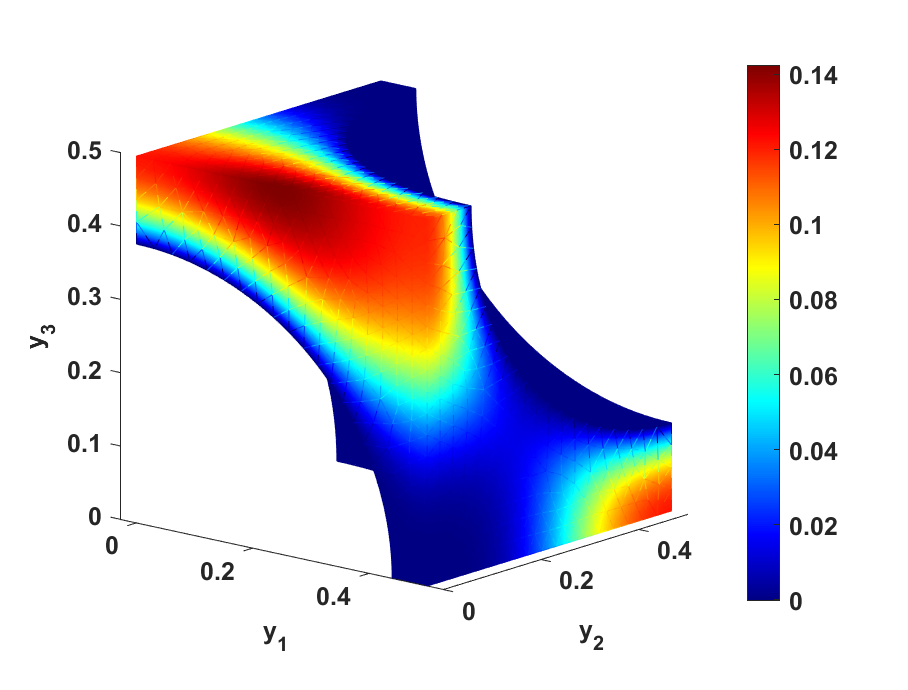
\includegraphics[width=4.1cm,height=3.9cm]{1_1.eps}
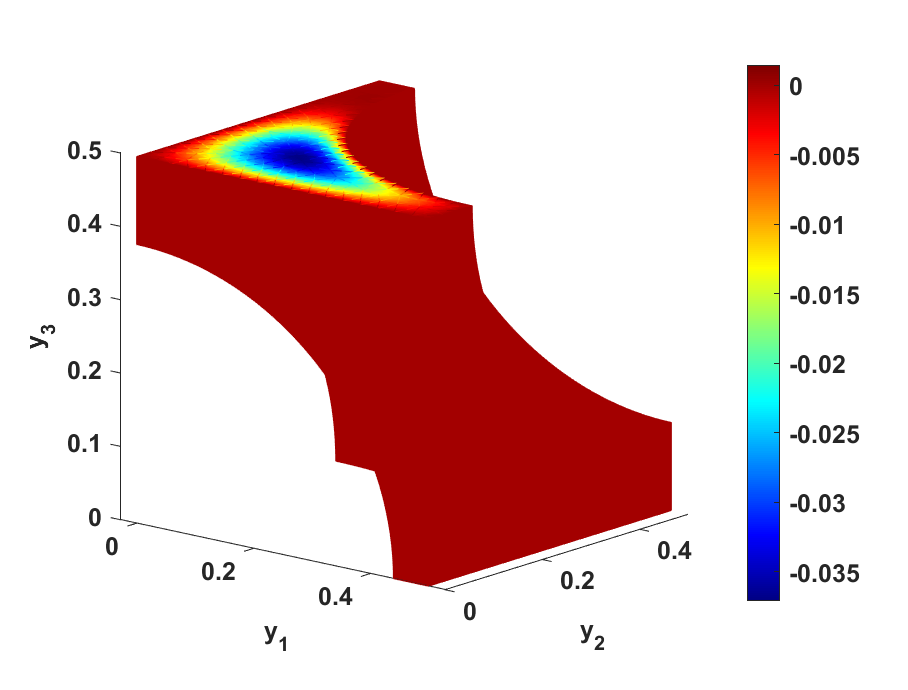
\includegraphics[width=4.1cm,height=3.9cm]{1_2.eps}
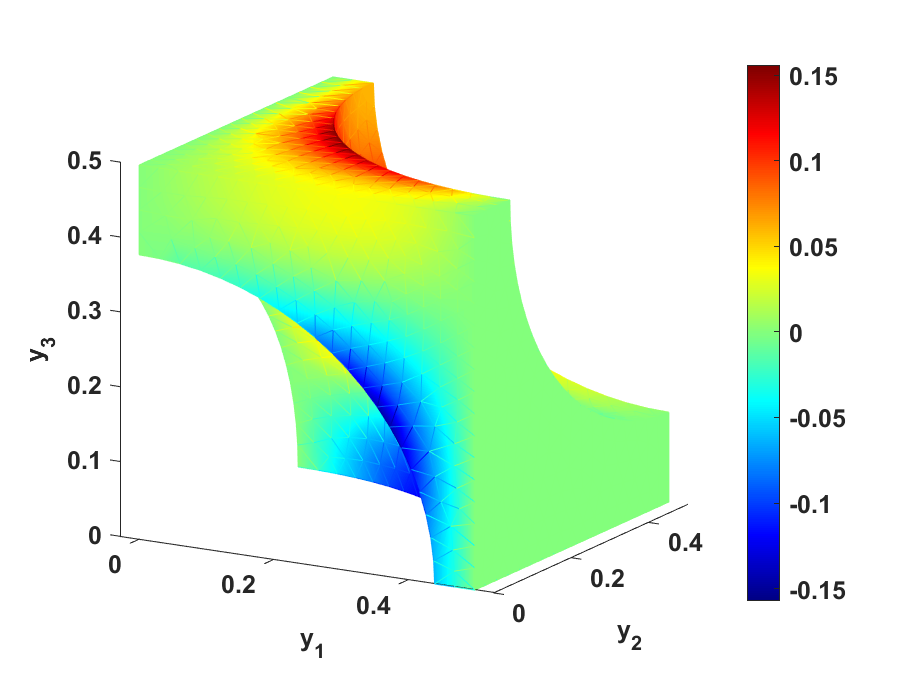
\includegraphics[width=4.1cm,height=3.9cm]{1_3.eps}
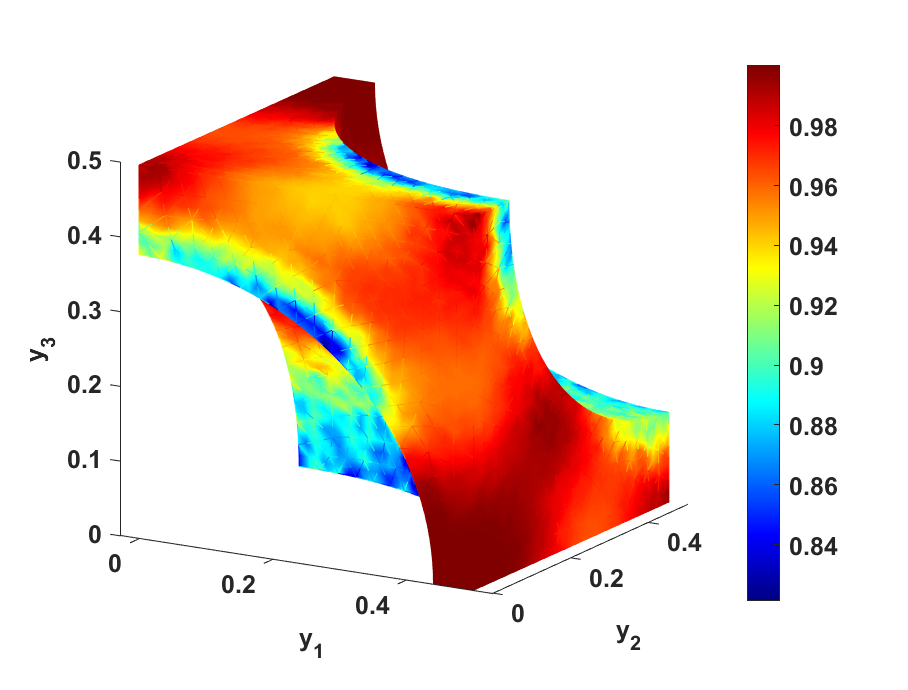
\includegraphics[width=4.1cm,height=3.9cm]{1_4.eps}\\
$(a)$\ velocity $\tilde{V}_{1}^{(1)}$\quad
$(b)$\ velocity $\tilde{V}_{2}^{(1)}$\quad
$(c)$\ pressure pulse $\tilde{P}^{(1)}$\quad
$(d)$\ non-Newtonian viscosity $\tilde{\mu}^{(1)}$\\
\small{Figure 1. Numerical results for a local problem of Carreau-Yasuda fluid in 1/8 periodic cells.}
\end{figure}

The sensitivity of non Newtonian viscosity to permeability and effective viscosity was discussed through numerical simulation.
\begin{figure}[htp]
\centering
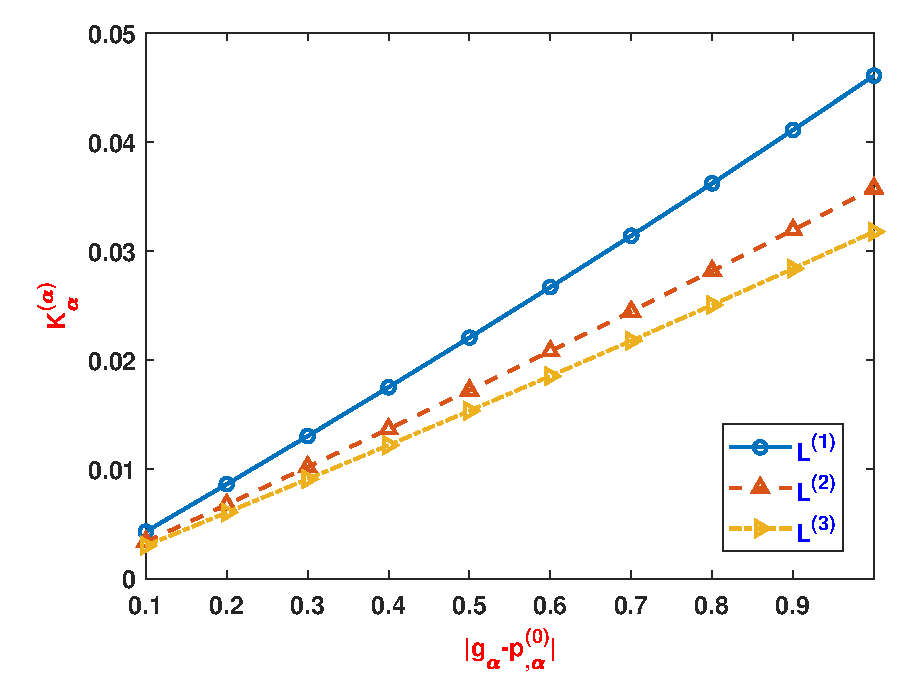
\includegraphics[width=6.4cm,height=4.2cm]{2_1.eps}
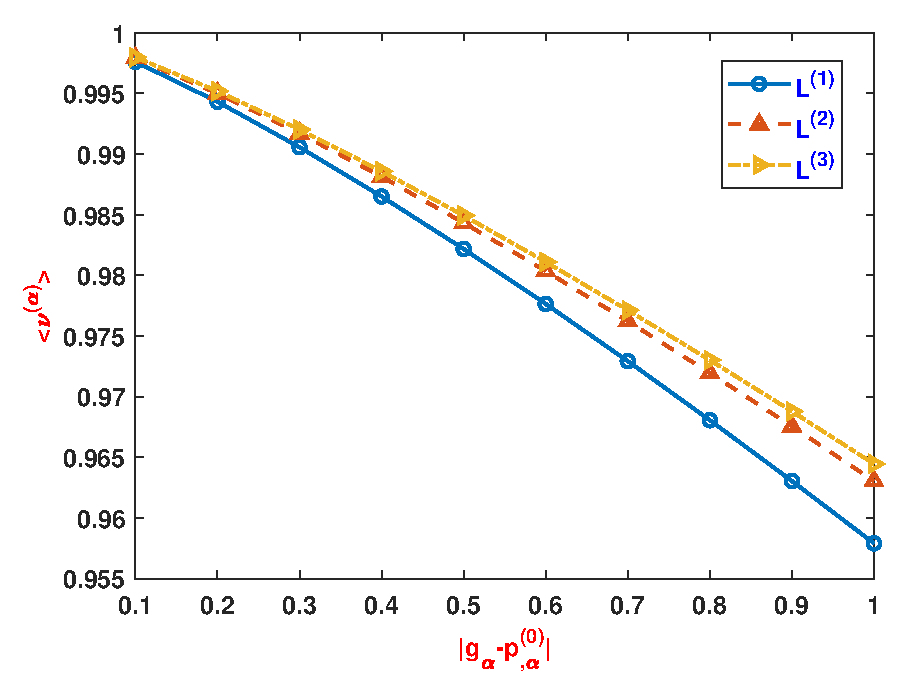
\includegraphics[width=6.4cm,height=4.2cm]{2_2.eps}\\
$(a)$\ changes in permeability tensor $K_{\alpha}^{\alpha}$\quad\quad\quad
$(b)$\ changes in effective viscosity $\mu^{(\alpha)}$\\
\small{Figure 2. The relationships between the permeability tensor $K_{\alpha}^{\alpha}$
and effective viscosity $\mu^{(\alpha)}$  of a Carreau-Yasuda fluid.}
\end{figure}

% The figures and tables are drawn according to the standard class 'article'.

\begin{thebibliography}{9} % or {99}, if there is more than ten references.
\bibitem{1} Li S.G., Dimitrienko Y.I.
    Mathematical modeling for the local flow of a generalized Newtonian fluid in 3D porous media.
    Appl. Math. Model.~2022. Vol.~105, Pp.~551--565. %https://doi.org/10.1016/j.apm.2022.01.003

\bibitem{2} Li S.G., Dimitrienko Y.I.
    Least squares finite element simulation of local transfer for a generalized Newtonian fluid in 2D periodic porous media.
    J. Non-Newton. Fluid Mech.~2023. Vol.~316, Pp.~105032. %https://doi.org/10.1016/j.jnnfm.2023.105032

\bibitem{3} Li S.G., Lv L.J., Liao M.Y. Numerical simulation of heat transfer and entropy generation due to the nanofluid natural convection with viscous dissipation in an inclined square cavity. Numer. Heat Transf. A Appl.~2024. %https://doi.org/10.1080/10407782.2024.2325121
\end{thebibliography}
%\end{document}

\end{englisharticle}

\begin{englisharticle}

\iffalse
\documentclass[12pt]{llncs}

\usepackage{todonotes}

\usepackage{nla} 

\begin{document}
\fi

\title{Spectral theory and asymptotic behavior of solutions for differential-algebraic equations\thanks{The research is supported by NAFOSTED, project No.~101.02-2021.43.}}

\author{Vu Hoang Linh
  }
\institute{VNU University of Science, Hanoi, Vietnam\\
  \email{linhvh@vnu.edu.vn}
  }

\maketitle

\begin{abstract}
The spectral theory (Lyapunov and Bohl exponents) for linear time-varying
ordinary differential equations (ODEs) and differential-algebraic equations (DAEs)
can be considered as generalizations of eigenvalue problems for
constant matrices and matrix pencils. The spectral theory can be used for characterizing
asymptotic behavior and stability of solutions. One of the most interesting problems 
is the investigation of Lyapunov/Bohl exponents of solutions when the system is
under small linear/nonlinear perturbations. These questions led to the stability of 
exponents and Perron theorems. In the last decade, some results were
extended from ODEs to DAEs and from the time-invariant case to the time-varying
one. First, we give a brief overview on the existing results. Next, we discuss some open problems 
in the operator setting that includes infinite dimensional systems modeled by partial differential-
algebraic (PDAEs) or delay-differential-algebraic equations (DDAEs).
\keywords{Differential-algebraic equations, Lyapunov exponents, Bohl exponents, stability of exponents}
\end{abstract}


%\end{document}

\end{englisharticle}

\begin{englishtitle} % Настраивает LaTeX на использование английского языка
% Этот титульный лист верстается аналогично.
\title{Problem of Control of transportation of elastic beams by carts composition in the presence of uncertainty}
% First author
\author{Nikita Livanov\inst{1} \and  Igor Izmestev\inst{2}
}
\institute{Chelyabinsk State University, Chelyabinsk, Russia\\
  \email{nikita.livanov.mail@gmail.com}
  \and
Chelyabinsk State University, Chelyabinsk, Russia\\
\email{j748e8@gmail.com}}
% etc

\maketitle

\begin{abstract}
We consider the problem of controlling a hyperbolic system that describes the stretching of $n$ elastic beams in a non-inertial reference frame during their transportation by a locomotive with a train of $n$ bogies. The control is the traction force of the locomotive, limited in magnitude. The uncertainty consists of the influence of external disturbances on each beam and the totality of forces opposing the movement of the locomotive. On each cart, one beam of length $l$ is rigidly attached to the right end. The left ends of the beams are not secured. The goal of choosing a control is to ensure that at a fixed moment in time the modulus of the linear function, determined using the average values of the beam tensions, does not exceed a given value for any acceptable realizations of uncertainty. A technique has been developed for reducing this problem to a one-dimensional control problem in the presence of uncertainty. Necessary and sufficient conditions for termination are found.

\keywords{control, hyperbolic system, guaranteed result, uncertainty} % в конце списка точка не ставится
\end{abstract}
\end{englishtitle}

\iffalse
%%%%%%%%%%%%%%%%%%%%%%%%%%%%%%%%%%%%%%%%%%%%%%%%%%%%%%%%%%%%%%%%%%%%%%%%
%
%  This is the template file for the 6th International conference
%  NONLINEAR ANALYSIS AND EXTREMAL PROBLEMS
%  June 25-30, 2018
%  Irkutsk, Russia
%
%%%%%%%%%%%%%%%%%%%%%%%%%%%%%%%%%%%%%%%%%%%%%%%%%%%%%%%%%%%%%%%%%%%%%%%%


\documentclass[12pt]{llncs}  

% При использовании pdfLaTeX добавляется стандартный набор русификации babel.

\usepackage{iftex}

\ifPDFTeX
\usepackage[T2A]{fontenc}
\usepackage[utf8]{inputenc} % Кодировка utf-8, cp1251 и т.д.
\usepackage[english,russian]{babel}
\fi

\usepackage{todonotes} 

\usepackage[russian]{nla}

\begin{document}
\fi

\title{Задача управления транспортировкой упругих балок составом тележек при наличии неопределенности }
% Первый автор
\author{Н.~Д.~Ливанов\inst{1} \and И.~В.~Изместьев\inst{2}
  \and
}

% Аффилиации пишутся в следующей форме, соединяя каждый институт при помощи \and.
\institute{Челябинский государственный университет (ФГБОУ ВО ЧелГУ), Челябинск, Россия \\
  \email{nikita.livanov.mail@gmail.com}
  \and   % Разделяет институты и присваивает им номера по порядку.
Челябинский государственный университет (ФГБОУ ВО ЧелГУ), Челябинск, Россия\\
  \email{j748e8@gmail.com}
% \and Другие авторы...
}

\maketitle

\begin{abstract}
Рассматривается задача управления гиперболической системой, которая описывает растяжение $n$ упругих балок  в неинерциальной системе отсчета во время их транспортировки локомотивом с составом из $n$ тележек. Управлением является ограниченная по величине сила тяги локомотива. Неопределенность складывается из воздействия внешних возмущений на каждую балку и совокупности сил противодействующих движению локомотива. На каждой тележке жестко закреплена за правый конец одна балка длины $l$. Левые концы балок не закреплены. Цель выбора управления заключается в том, чтобы в фиксированный момент времени модуль линейной функции, определяемой с помощью средних величин растяжений балок, не превышал заданного значения при любых допустимых реализациях неопределенности. Разработана методика сведения данной задачи к одномерной задаче управления при наличии неопределенности. Найдены необходимые и достаточные условия окончания.


\keywords{управление, гиперболическая система, гарантированный результат, неопределенность} % в конце списка точка не ставится
\end{abstract}

Зададим систему $n$ уравнений продольных колебаний в неинерциальной системе отсчета [1], описывающих транспортировку упругих балок на составе тележек локомотивом:  
\begin{eqnarray} \label{eq:sVJ}
\frac{\partial^2 U_i(t,x)}{\partial t^2} = \frac{\partial^2 U_i(t,x)}{\partial x^2} + f_i(t,x)-\rho(F(t)-W(t)), \quad i=\overline{1,n},
\end{eqnarray} 
где $0\leq t \leq p$ и $0\leq x \leq l$, функции $U_i(t,x)$, $i=\overline{1,n}$ описывают изменение растяжения балок, число $\rho \in (0;1)$. Система (1) рассматривается при заданных начальных условиях
$$
U_i(0,x) = g_i(x), \quad \frac{\partial U_i(0,x)}{\partial t} = G_i(x), \quad i= \overline{1,n},
$$
где функции $g_i(x), G_i(x)$ $i= \overline{1,n}$ являются непрерывными. Плотность совокупности внешних сил, действующих на $i$-балку, задается непрерывной функцией $f_i(x,t)$. Из условий того, что правый конец каждой балки жестко закреплен, а левый свободен, следует, что граничные условия принимают вид 
$$
U_i(t,l) = 0,\quad \frac{\partial U_i(t,0)}{\partial x} = 0,\quad i= \overline{1,n}. 
$$
Считаем, что на локомотив воздействует сила тяги $F(t)$ и внешние силы препятствующие движению $W(t)$ [2], которые изменяются согласно уравнениям
\begin{eqnarray} \label{eq:U}
    F(t) = a_1(t) + b_1(t)\xi(t), \quad |\xi(t)|\leq 1,
    \\\label{eq:P}
    W(t) = a_2(t) + b_2(t)\eta(t), \quad |\eta(t)|\leq 1.
\end{eqnarray}
Функции $a_j(t)$, $b_j(t)\geq 0$, $j= 1,2$, непрерывны при $t \in [0,p]$; $\xi(t)$ и $\eta(t)$ являются управлением и помехой, соответственно.

Известны оценки непрерывных функций $f_i(t,x)$:
\begin{eqnarray} \label{eq:f_i}
    \hat{f}_i(t,x)\leq f_i(t,x) \leq \tilde{f}_i(t,x), \quad i=\overline{1,n}
\end{eqnarray}
Функции $\hat{f}_i(t,x)$, $\tilde{f}_i(t,x)$ являются непрерывными.
Заданы числа $\alpha \in \mathbb{R}$, $\varepsilon \geq 0$ и вектор $\overline{\lambda} = (\lambda_1, \lambda_2, \ldots, \lambda_n)^\top \in \mathbb{R}^n$ такой, что $\overline{\lambda} \neq \overline{0}$. Цель выбора управления  $\xi(t)$ (2) заключается в том, чтобы осуществить неравенство 
\begin{eqnarray} \label{eq:Cel}
    \left| \sum_{i=1}^n \lambda_i\int_0^l \left(U_i(t,x)\sigma(x) \right) dx - \alpha\right | \leq \varepsilon
\end{eqnarray}
для любой реализации помехи $\eta(t)$ (3) и для любых непрерывных функций $f_i(t,x)$ (4), $i=\overline{1,n}$. Здесь $\sigma: [0,1] \to \mathbb{R}$ заданная непрерывная функция, удовлетворяющая условиям
$\sigma(0)=\sigma(l) = 0$.


После замены переменных задача (1)--(5) сводится к одномерной однотипной задаче управления при наличии неопределенности [3]:
\begin{eqnarray} \label{eq:Y1}
    \dot{z} = -a(t)u+b(t)v,  \quad |u|\leq1,\quad |v|\leq 1, \quad |z(p)|\leq \varepsilon.
\end{eqnarray}

Здесь $u$~--- одномерное управление, $v$~--- неопределенность; функции $a(t) \geq 0$,  $b(t) \geq 0$ являются непрерывными при $t \leq p$.

Используя метод оптимизации гарантированного результата \cite{Kras}, найдены необходимые и достаточные условия окончания в задаче (6). Кроме того, построено соответствующее управление $\xi$, решающее задачу (1)--(5).









\begin{thebibliography}{9} % или {99}, если ссылок больше десяти.
\bibitem{Koshlyakov} Кошляков~Н.С. Основные дифференциальные уравнения математической физики. ОНТИ,~1936.

\bibitem{Frolov} Фролов~Н.О. ТЯГА ПОЕЗДОВ~/Конспект лекций
по дисциплине «Тяга поездов» для студентов. Екатеринбург:~ УрГУПС,~2020.

\bibitem{Uxobotov} Ухоботов~В.И. Метод одномерного проектирования в линейных дифференциальных играх с интегральными ограничениями~/ Учеб. пособие. Челябинск:~Челябинский государственный университет,~2005.

\bibitem{Kras} Красовский~Н.Н. Управление динамической системой. М.:~Наука,~1985.


\end{thebibliography}

% После библиографического списка в русскоязычных статьях необходимо оформить
% англоязычный заголовок.




%\end{document}




\begin{englishtitle} % Настраивает LaTeX на использование английского языка
% Этот титульный лист верстается аналогично.
\title{On the stability of solutions to the variational \\ Prony problem\thanks{The study was carried out within the framework of the state contract of the Sobolev Institute of Mathematics (project no. FWNF-2022-0008)}}
% First author
\author{Andrei Lomov
}
\institute{Sobolev Institute of Mathematics, Novosibirsk State University, \\ Novosibirsk, Russia, \email{lomov@math.nsc.ru}
}
% etc

\maketitle

\vspace{-1ex}
\begin{abstract}
Using the Mean value theorem, new
stability constants of solutions to the variational Prony problem are obtained.

\keywords{the variational Prony problem, local stability, guaranteed estimates} % в конце списка точка не ставится
\end{abstract}
\end{englishtitle}

\iffalse
%%%%%%%%%%%%%%%%%%%%%%%%%%%%%%%%%%%%%%%%%%%%%%%%%%%%%%%%%%%%%%%%%%%%%%%%
%
%  This is the template file for the 6th International conference
%  NONLINEAR ANALYSIS AND EXTREMAL PROBLEMS
%  June 25-30, 2018
%  Irkutsk, Russia
%
%%%%%%%%%%%%%%%%%%%%%%%%%%%%%%%%%%%%%%%%%%%%%%%%%%%%%%%%%%%%%%%%%%%%%%%%


\documentclass[12pt]{llncs}  

% При использовании pdfLaTeX добавляется стандартный набор русификации babel.

\usepackage{iftex}

\ifPDFTeX
\usepackage[T2A]{fontenc}
\usepackage[utf8]{inputenc} % Кодировка utf-8, cp1251 и т.д.
\usepackage[english,russian]{babel}
\fi

\usepackage{todonotes} 

\usepackage[russian]{nla}

\begin{document}
\fi
\title{Об устойчивости решений вариационной задачи Прони\thanks{Работа выполнена в рамках государственного задания Института математики им. С.Л. Соболева СО РАН, проект \textnumero~FWNF-2022-0008}}
% Первый автор
\author{А.~А.~Ломов
}

% Аффилиации пишутся в следующей форме, соединяя каждый институт при помощи \and.
\institute{ИМ СО РАН им. С.Л. Соболева, Новосибирский государственный университет, \\ Новосибирск, Россия,
  \email{lomov@math.nsc.ru}
}

\maketitle

\begin{abstract}
По теореме об оценке конечных приращений получены новые константы
устойчивости решений вариационной задачи Прони.

\keywords{вариационная задача Прони, локальная устойчивость, гарантированные оценки} % в конце списка точка не ставится
\end{abstract}

\newcommand{\T}{\top}

\section{Основные результаты} % не обязательное поле

Вариационной задачей Прони называем обратную задачу идентификации
вектора параметров $\theta\in\mathbb{R}^{v}$ разностного уравнения
\begin{equation}
\alpha_{n}x_{k+n}+\alpha_{n-1}x_{k+n-1}+\ldots+\alpha_{0}x_{k}=0,\quad k=\overline{1,N-n},\label{SL/eq:RU}
\end{equation}
с матричными коэффициентами $\alpha_{i}=\alpha_{i}(\theta)\in\mathbb{R}^{r\times\left(r+m\right)}$,
$i=\overline{0,n}$ по возмущенным наблюдениям
$y=x+\delta x\in\mathbb{R}^{N\left(r+m\right)}$
процесса $x\doteq\left[x_{1};\ldots;x_{N}\right]$. Предполагается,
что $\alpha=D\theta+d$, где $\alpha\doteq\mathrm{vect}\left[\alpha_{0};\ldots;\alpha_{n}\right]$,
столбцы $\left[D,d\right]$ линейно независимы, и задача вычисления $\theta$ по $x$ однозначно разрешима.

Устойчивость решений
$\hat{\theta}(x+\delta x)=\theta+\delta\theta$
к возмущениям зависит от целевой функции; при аддитивных возмущениях предпочтительна \cite{Lomov--Rusinova-2022} вариационная ЦФ:
\[
\hat{\theta}=\arg\min_{\theta}J(\theta,y),\quad J(\theta,y)\doteq\left\Vert y-\hat{x}(\theta)\right\Vert ^{2},\quad\hat{x}(\theta)\doteq\left(I-GCG^{\T}\right)y,\quad C\doteq\left(G^{\T}G\right)^{-1},
\]
где $G^{\T}\doteq\left\backslash \alpha(\theta)\right\backslash $ есть клеточно-теплицевая
матрица системы уравнений \eqref{SL/eq:RU}.

Нас интересуют гарантированные границы для нормы отклонений
$\left\Vert \delta\theta\right\Vert $,
в отличие от анализа с точностью до малых более высоких порядков \cite{Abatzoglu-et-al-1991}.

\smallskip
\textbf{Теорема (об оценке конечных приращений)}
\textsl{
Пусть отображение $F:\Omega\to\mathbb{R}^{v}$ непрерывно
дифференцируемо в выпуклой компактной области пространства
$\mathbb{R}^{N\left(r+m\right)}$.
Тогда $\left\Vert F(y)-F(x)\right\Vert \leq\sup_{\xi\in\Omega}\left\Vert F^{\prime}(\xi)\right\Vert \cdot\left\Vert y-x\right\Vert $.
}\smallskip


Для неявной функции $\hat{\theta}(y)\doteq F(y)$, вычисляемой из
условия $J_{\theta}^{\prime}(\hat{\theta},y)=0$, имеем производную Фреше
$F^{\prime}=-\left(J_{\theta\theta}^{\prime\prime}\right)^{-1}J_{\theta y}^{\prime\prime}\doteq S^{\T}$.
Пусть $\|\cdot\|$ — операторная норма, тогда
\[
\|F^{\prime}(y)\|=\|S(\hat{\theta}(y),y)\|=\lambda_{\text{max}}^{1/2}\left(S^{\T}S\right).
\]

\smallskip
\textbf{Лемма.}\textsl{
При возмущении $R\to R+\Delta R\in\mathbb{R}^{n}$ симметричной положительно определенной матрицы $R$ верна гарантированная оценка для наименьшего
собственного числа $\lambda_{i}\doteq\lambda_{i}\left(R\right)$,
$\lambda_{1}<\lambda_{2}\leq\ldots\leq\lambda_{n}$
($\left\Vert \cdot \right\Vert_{F} $ --- фробениусовская норма):
\[
\lambda_{1}+\Delta\lambda_{1}\in\left[\lambda_{1}\pm\left(\left\Vert \Delta R\right\Vert _{F}+\frac{2n}{\left|\lambda_{2}-\lambda_{1}\right|}\left\Vert \Delta R\right\Vert _{F}^{2}\right)\right].
\]
}\smallskip

\textbf{Предложение.}\textsl{
В вариационной задаче Прони
$S^{\T}S=\left(D^{\T}\hat{V}^{\T}C\hat{V}D\right)^{-1}\doteq R^{-1}$,
где $\hat{V}$ есть клеточно-ганкелевая матрица из отсчетов процесса
$\hat{x}$: $G^{\T}\hat{x}\equiv\hat{V}\left(D\theta+d\right).$ Тогда
$\lambda_{\mathrm{max}}^{1/2}\left(S^{\T}S\right)=\lambda_{\mathrm{min}}^{-1/2}\left(R\right).$
}\smallskip

Как следствие теоремы об оценке конечных приращений имеет место неравенство
\(
\|\delta\theta\| \leq\frac{\varepsilon}{\inf_{\|\delta x\|\leq\varepsilon,\;\left\Vert \delta\theta\right\Vert \leq\mu\varepsilon\lambda_{\mathrm{min}}^{-1/2}\left(R\right)}\,\lambda_{\mathrm{min}}^{1/2}\left(R\right)},
\)
где $\mu\geq1$ — априорный коэффициент.

\smallskip
\textbf{Теорема.}\textsl{
В вариационной задаче Прони верна следующая гарантированная оценка для ошибки вектора параметров: $\left\Vert \delta\theta\right\Vert \leq\mu\frac{\varepsilon}{\sqrt{\lambda_{1}}},\quad\mu\geq1,$
$\lambda_{1}\doteq\lambda_{\mathrm{min}}\left(R\right)$,
при техническом условии
$\varepsilon\leq\frac{\left(\sqrt{2}-1\right)}{5n\left\Vert D\right\Vert ^{2}\left\Vert V\right\Vert ^{2}\left\Vert C\right\Vert ^{3/2}}\cdot\frac{\left(1-\mu^{-2}\right)\lambda_{1}^{3/2}}{\left(\mu+\frac{3\sqrt{n+1}}{5n\left\Vert x\right\Vert \left\Vert C\right\Vert ^{1/2}}\sqrt{\lambda_{1}}\right)}.$
}\smallskip

Проведены расчеты для границ нормы ошибки
$\left\Vert \delta\theta\right\Vert $
в задаче Ланцоша восстановления экспоненциальных слагаемых из возмущенных наблюдений суммы трех экспонент \cite{Lanczos-1956} и на ряде более обусловленных примеров. Показано, что ранее полученные границы нормы
ошибки $\left\Vert \delta\theta\right\Vert $ (ссылки в \cite{Lomov--Rusinova-2022,Lomov-2024-MTrudy}),
основанные на оценках остаточного члена второго порядка в разложении в ряд Тейлора неявной функции $\hat{\theta}(y)$ (по сути на оценках конечных приращений производной Фреше), на несколько порядков менее эффективны, как и оценки на основе неравенств типа Уилкинсона.

% В конце текста можно выразить благодарности, если этого не было
% сделано в ссылке с заголовка статьи, например,
% Работа выполнена при поддержке РФФИ (РНФ, другие фонды), проект \textnumero~00-00-00000.
%



\begin{thebibliography}{9} % или {99}, если ссылок больше десяти.
\bibitem{Lomov--Rusinova-2022}\emph{Ломов\,А.\,А., Русинова\,Е.\,А.}
Сравнение целевых функций в задаче Прони для аппроксимации данных
измерений // Вестник ЮУрГУ. Серия «Вычислительная математика и информатика».
2022. Т. 11, № 2. С. 18-27. DOI: 10.14529/cmse220202

\bibitem{Abatzoglu-et-al-1991}\emph{Abatzoglu\,T.J., Mendel\,J.M.,
Harada\,G.A.} The Constrained Total Least Squares Technique and its
Applications to Harmonic Superresolution // IEEE Trans. Signal Processing.
1991. V.\,SP-39. P.\emph{\,}1070-1087.

\bibitem{Lanczos-1956}\emph{Lanczos\,C}. Applied analysis. Prentice
Hall, Englewood Cliffs, N.J., 1956. 539\,p. Пер.: \emph{Ланцош\,К}.
Практические методы прикладного анализа. М.: ФМЛ, 1961. 524\,с.

\bibitem{Lomov-2024-MTrudy}\emph{Ломов\,А.А}. О локальной устойчивости
в полной задаче Прони // Математические труды. №1. 2024. Принято к
публикации.

\bibitem{VanHuffel--Vandewalle-1991}\emph{Van\,Huffel\,S., Vandewalle\,J}.
The total least squares problem. SIAM, Philadelphia, 1991.

\end{thebibliography}

% После библиографического списка в русскоязычных статьях необходимо оформить
% англоязычный заголовок.






%\end{document}



\begin{englisharticle}

\iffalse
\documentclass[12pt]{llncs}

\usepackage{todonotes}

\usepackage{nla} 

\begin{document}
\fi

\title{Optimal control of the economic system in conditions of mass disease with vaccination\thanks{The research was financially supported by the Russian Science Foundation No. 24-28-00542, https://rscf.ru/en/project/24-28-00542/}}

\author{Igor Lutoshkin  \and   Maria Rybina
}
\institute{Ulyanovsk State University, Ulyanovsk, Russian Federation\\
  \email{lutoshkiniv@ulsu.ru}}

\maketitle

\begin{abstract}
The development of a model for managing the economic system in conditions of mass disease is proposed. A special feature of this model is the simultaneous consideration of socio-biological and socio-economic factors. In the model, control influences include costs for: construction of hospitals, refurbishment of existing beds, conducting an information campaign, vaccination. The model is formulated in terms of an optimal control problem with delay.

\keywords{optimal control, economic system, mass disease, vaccination}
\end{abstract}


\section{The model} %optional section

Mathematical modeling of the development of mass disease has resulted in a number of models aimed mainly at predicting, for example, \cite{BraurCastChav2012,Gets2018,SietRus2013}. Control models have also been proposed \cite{GomRubMon2023,LueGPCerv2023,CastBlowDri2002}.  They are formulated in terms of optimal control problems. At the same time, these models are medical and/or biological; they poorly reflect social indicators.

The works \cite{LutoshRyb2023,LutoshRyb2023_2} proposed a mathematical model for managing a socio-economic system in conditions of a mass disease. It simultaneously takes into account socio-biological and economic factors. The present study is aimed at developing the model proposed in \cite{LutoshRyb2023,LutoshRyb2023_2} by adding a vaccination factor.

Let $P$ -- number of people complying with restrictions measures; $S$ -- number of people who do not comply with restrictive measures; $E$ -- number of infected people; $I$ -- number of sick people; $Q$ -- number of hospitalized people; $R$ -- number of recovered; $D$ -- number of deaths; $Z$ -- number of beds; $V_i$ -- number of people who have received artificial immunity to the disease due to being vaccinated with the vaccine $i$, $i=\overline{1,n}$; $N$ -- population size; $Y$ -- gross output; $\pi$ -- profit; $K$ -- cost of fixed assets; $L$ -- representation of the working population. Control variables: $u_1$ -- intensity of costs for refurbishment of existing beds; $u_2$ -- cost intensity for the construction of new hospitals; $u_3$ -- intensity of costs for the information campaign; $u_{3+i}$ -- intensity of costs for a campaign to vaccinate the population with the vaccine $i$, $i=\overline{1,n}$.

Let's introduce differential equations:
$$\begin{array}{c}
   \displaystyle\frac{dS}{dt}=k_{PS}P(t)+k_{RS}R(t-\tau)- \left(k_{SE}\left(\frac{I(t)}{N(t)}\right)+k_{SP}(u_3(t))-\rho\right)S(t)+\\ \displaystyle\sum_{i=1}^{n}V_i(t-\widetilde{\tau_i})- \sum_{i=1}^{n}\frac{u_{3+i}(t-\widehat{\tau_i})}{c_i}; \\ \displaystyle\frac{dP}{dt}=k_{SP}(u_3(t))S(t)-k_{PS}P(t); \\ \displaystyle\frac{dE}{dt}=k_{SE}\left(\frac{I(t)}{N(t)}\right) \left(S(t)+\sum_{i=1}^{n}(1-\widetilde{e_i}\frac{u_{3+i}(t-\widehat{\tau_i})}{c_i}) \right)-k_{EI}E(t);
\end{array}$$  

$$\begin{array}{c}
   \displaystyle\frac{dI}{dt}= k_{EI}E(t)-(k_{IQ}+k_{IR}+k_{ID})I(t); \quad \displaystyle\frac{dQ}{dt}= k_{IQ}I(t)-(k_{QD}+k_{QR})Q(t);\\ \displaystyle\frac{dR}{dt}= k_{IR}I(t)+k_{QR}Q(t)-k_{RS}R(t); \quad \displaystyle\frac{dD}{dt}= k_{QD}Q(t)+k_{ID}I(t);\\
   \displaystyle\frac{dZ}{dt}= g(u_2(t-\tilde{\tau}))-\mu Z(t)+ku_1(t); \\
   \displaystyle\frac{dV_i}{dt}= \left(1-(1-\widetilde{e_i})k_{SE}\left(\frac{I(t)}{N(t)}\right)\right) \frac{u_{3+i}(t-\widehat{\tau_i})}{c_i}-V_i(t-\widetilde{\tau_i}),\quad i=\overline{1,n}.
  \end{array}
$$

Let's take into account the vaccination factor in the algebraic connections:  $Q(t)\leq Z(t)$; $L(t)=\displaystyle m\left(e_PP(t)+e_SS(t)+e_EE(t)+e_RR(t)+\sum_{i=1}^{n}e_{V_i}V_i(t)\right)$; $N(t)=P(t)+S(t)+E(t)+I(t)+Q(t)+R(t)+\displaystyle\sum_{i=1}^{n}V_i(t)$;
$Y(t)=F(K(t),L(t))$; $\pi(t)=Y(t)-\displaystyle\sum_{i=1}^{n+3}u_i(t)$;
$u_i(t)\geq 0$, $\displaystyle\int_{t_0}^T u_i(t)dt\leq B_i$, $i=\overline{1,n+3}$. 

The functional can be represented as
$$J=\min_{u_1,...,u_{n+3}}\int_{0}^{T}\left(\alpha_1\frac{E(t)}{N(0)}-\alpha_2\frac{\pi(t)}{Y(0)}\right)dt.$$
Here $\alpha_1+\alpha_2=1$.


\begin{thebibliography}{9} % or {99}, if there is more than ten references.

\bibitem{BraurCastChav2012} Brauer~F., Castillo-Chavez~C. Mathematical models in population biology and epidemiology. 2012. Vol.~40. New York, Springer. 508~p.

\bibitem{Gets2018} Modeling epidemics: A primer and Numerus Model Builder implementation / W.~M.~Getz, R.~Salter, O.~Muellerklein [et al.].  Epidemics. 2018.  Vol.~25.  Pp.~9–19. https://doi.org/10.1016/j.epidem.2018.06.001

\bibitem{SietRus2013} Siettos~C.~I., Russo~L. Mathematical modeling of infectious disease dynamics. Virulence. Taylor and Francis Inc, 2013.  Vol.~4. no~4. Pp.~295–306.

\bibitem{GomRubMon2023} Gomez~M.~C., Rubio~F.~A., Mondragon~E.~I. Qualitative analysis of generalized multistage epidemic model with immigration // Mathematical Biosciences and Engineering. 2023. Vol.~20. Iss.~9. Pp.~15765-15780.  https://doi.org/10.3934/mbe.2023702

\bibitem{LueGPCerv2023} Luebben~G., Gonzalez-Parra~G.,  Cervantes~B. Study of optimal vaccination strategies for early COVID-19 pandemic using an age-structured mathematical model:  A case study of the USA // Mathematical Biosciences and Engineering, 2023. Vol.~20. Iss.~6. Pp.~10828-10865.  https://doi.org/10.3934/mbe.2023481

\bibitem{CastBlowDri2002} Mathematical Approaches for Emerging and Reemerging Infectious Diseases: Models, Methods and Theory, Edited by Castillo-Chavez~C. with S.~Blower P.~van~den~Driessche, D.~Kirschner, A.~A.~Yakubu. New York, Springer, 2002. 377~p. https://doi.org/10.1007/978-1-4613-0065-6.

\bibitem{LutoshRyb2023} Lutoshkin~I.~V., Rybina~M.~S. Modelling of Regional Economic Management in Conditions of Mass Diseases.  Economy of regions, 2023, Vol.~19, no.~2, Pp.~299-313. https://doi.org/10.17059/ekon.reg.2023-2-1 [in Russian]

\bibitem{LutoshRyb2023_2} Lutoshkin~I.~V., Rybina~M.~S. Optimal solution in the model of control over an economic system in the condition of a mass disease. Izvestiya of Saratov University.  Mathematics. Mechanics. Informatics, 2023, Vol.~23, no.~2, Pp.~264-273. https://doi.org/10.18500/1816-9791-2023-23-2-264-273

\end{thebibliography}
%\end{document}

\end{englisharticle}

\begin{englisharticle}

\iffalse
%%%%%%%%%%%%%%%%%%%%%%%%%%%%%%%%%%%%%%%%%%%%%%%%%%%%%%%%%%%%%%%%%%%%%%%%
%
% This is the template file for the 6th International conference
% NONLINEAR ANALYSIS AND EXTREMAL PROBLEMS
% June 25-30, 2018
% Irkutsk, Russia
%
%%%%%%%%%%%%%%%%%%%%%%%%%%%%%%%%%%%%%%%%%%%%%%%%%%%%%%%%%%%%%%%%%%%%%%%%
% The preparation of the article is based on the standard llncs class
% (Lecture Notes in Computer Sciences), which is adjusted with style
% file of the conference.
%
% There are two ways of compilation of the file into PDF
% 1. Use pdfLaTeX (pdflatex), (LaTeX+DVIPS will not work);
% 2. Use LuaLaTeX (XeLaTeX will work too).
% When using LuaLaTeX You will need TTF or OTF CMU fonts
% (Computer Modern Unicode). The fonts are installed with 'cm-unicode' package in
% a distribution of LaTeX % (https://www.ctan.org/tex-archive/fonts/cm-unicode),
% either by downloading and installing these fonts system wide, the address of their page is
% http://canopus.iacp.dvo.ru/%7Epanov/cm-unicode/
% The second option won't work in XeLaTeX.
%
% For MiKTeX (LaTeX distribution for Windows),
%  1. Package 'cm-unicode' is installed manually with the MiKTeX administration Console.
%  2. For the compilation of this example, namely, the stub figure, one will also need to
% download package 'pgf' manually. This package uses in the popular
% package tikz.
%  3. Tests showed that the rest of the required packages MiKTeX loads automatically (if
%     it is allowed). The 'auto download' option is
%     configured in 'Settings' section in MiKTeX Console.
%
%
% The easiest way to compile an article is to use pdfLaTeX, but
% the final layout of the book will be compiled with LuaLaTeX,
% as a result will be of better quality thanks to the package 'microtype' and
% use vector OTF instead of standard raster fonts of pdfLaTeX.
%
% In the case of questions and problems with the article compilation,
% write letters to e-mail: eugeneai@irnok.net, Cherkashin Evgeny.
%
% New version of the correcting style file will be available at the website:
%     https://github.com/eugeneai/nla-style
%     file - nla.sty
%
% Further instructions are in the text body of the template. The template itself
% is an article example.
%
% The LaTeX2e format is used!

% 12 points font size is used.
\documentclass[12pt]{llncs}

% The correcting style file is added.
\usepackage{todonotes}

\usepackage{nla} % This package is needed for compiling
                 % this template, it should be removed
                 % from your article.

% Many popular packages (amsXXX, graphicx, etc.) are already imported in the style file.
% If there is a conflict with your packages, try disabling them and compile
% the text.
%
% It would be convenient in the layout of the proceedings if the file names
% of the figures of different authors do not clash.
% To minimize the clash, the drawings can be placed in a separate subfolder
% named after the author or the title of the paper.
%
% \graphicspath{{ivanov-petrov-pics/}} % specifies the folder with images in png, pdf formats.
% or
% \graphicspath{{great-problem-solving-paper-pics/}}.

%\usepackage{float}
\begin{document}
\fi
% Text should be formatted in accordance with the 'article' class, using extensions like
% AMS.
%
\title{The effects of viscous dissipation on the nanofluid natural convection in a tilted square cavity\thanks{The research is supported by partially by the  Natural Science Foundation of Liaoning Province in China, project No.~2022-BS-093, the  Fundamental Research Funds for the Central Universities of China, project No.~3132023203 and  the Educational Science Planning Projects of Liaoning Province of China, project No.~JG21DB065. }}
% First author
\author{Longjie Lv\inst{1} \and Shuguang Li\inst{2} \and  Mingyue Wei\inst{3}
}
\institute{School of Science, Dalian Maritime University, Dalian,  China\\
  \email{1783572186qq@dlmu.edu.cn}
  \and
School of Science, Dalian Maritime University, Dalian,  China\\
\email{shuguangli2008@126.com}
\and
School of Science, Dalian Maritime University, Dalian,  China\\
\email{w15633860221@163.com}}
% etc

\maketitle

\begin{abstract}
The viscous dissipation  leads to changes in the temperature, viscosity, heat transfer and other physical properties of the fluid during the flow process, thereby affecting the flow characteristics.
And it plays an important role in damping effect, momentum transfer and energy dissipation. Therefore, more in-depth research is needed to reveal the importance of viscous dissipation in natural convection.
In this work, the effects of viscous dissipation on the flow and heat transfer of nanofluid natural convection in a tilted square cavity are numerically studied by applying a newly proposed fractional-step semi-implicit algorithm with the numerical advantage of larger time steps. The cavity is filled with water and nanoparticles of copper ($Cu$), and the viscous dissipative behavior of the mixture flow is not negligible. This study has been conducted for certain pertinent parameters of Rayleigh number ($Ra = 10^{4}$ and $10^{5}$), Prandtl number ($Pr = 6.2$), Eckert number ($Ec$ = 0 $-$ 2), the volume fraction of solid particles ($\phi$ = 0 $-$ 0.06), and inclination angle of square cavity ($\alpha$ = 0 $-$ $\pi/2$).
\keywords{Natural convection,  Heat transfer, Nanofluid, Viscous dissipation, Fractional-step semi-implicit algorithm.}
\end{abstract}

% at the end of the list, there should be no final dot
%\section{The main results}


The results show that at any tilt angle , the increase in viscous dissipation leads to weakened heat transfer on the hot wall, enhanced heat transfer on the cold wall, and weakened flow in the square cavity. Adding solid particles can effectively weaken the effect of viscous dissipation. As the Rayleigh number increases, the effect of viscous dissipation increases. As the tilt angle increases, the effects of volume fraction and Eckert number weaken.

% The figures and tables are drawn according to the standard class 'article'.
\begin{figure}[htb]
 \centering
\vspace{-4cm}  
\setlength{\abovecaptionskip}{-3.cm}  
%% Two picture formats are supported:
\includegraphics[width=0.48\linewidth]{1.eps} % Raster format
\includegraphics[width=0.48\linewidth]{2.eps} % Vector and raster format
\caption{The effect of Eckert number on the average Nusselt number $Nu_{0}$ on the hot wall and the average Nusselt number $Nu_{1}$ on the cold wall with different volume fractions of the solid particles $\phi$ in a horizontally placed square cavity($\alpha$ = 0) at $Ra$ = $10^{5}$ }
%
% Vector drawings can be drawn in Inkscape editor
% https://inkscape.org/ru/download/
% The usual format of the editor is SVG, so the drawings must be exported in
% PDF or PNG (with a resolution of minimum 150 dpi, and maximum of 300 dpi).
  %\begin{center}
   % \missingfigure[figwidth=0.7\linewidth]{Remove me from the article!} \end{center}
  %\caption{Caption of the figure}\label{fig:example}
\end{figure}
The numerical results in Fig 1 show that for any solid particle volume fraction, viscous dissipation leads to reduced heat transfer on the hot wall and enhanced heat transfer on the cold wall. And as the volume fraction of solid particles increases, the effect of Eckert number on  heat transfer weakens.
\begin{figure}[htb]
 \centering
\vspace{-3.5cm}   
\setlength{\abovecaptionskip}{-3.cm}  
%% Two picture formats are supported:
\includegraphics[width=0.48\linewidth]{3.eps} % Raster format
\includegraphics[width=0.48\linewidth]{4.eps} % Vector and raster format
\caption{The effect of inclination angle $\alpha$ on the average Nusselt number $Nu_{0}$ on the hot wall and the average Nusselt number $Nu_{1}$ on the cold wall at $Ra$ = $10^{5}$}
%
% Vector drawings can be drawn in Inkscape editor
% https://inkscape.org/ru/download/
% The usual format of the editor is SVG, so the drawings must be exported in
% PDF or PNG (with a resolution of minimum 150 dpi, and maximum of 300 dpi).
  %\begin{center}
   % \missingfigure[figwidth=0.7\linewidth]{Remove me from the article!} \end{center}
  %\caption{Caption of the figure}\label{fig:example}
\end{figure}
The numerical results in Fig 2 show that as the tilt angle increases, the effects of solid particle volume fraction and Eckert number weaken.
% At the end of the text, acknowledgments are expressed, if you haven't
% made a footnote from the title. For example, we can write

\begin{thebibliography}{9} % or {99}, if there is more than ten references.
\bibitem{LiLv2024} Li S.G., Lv L.J., Liao M.Y. Numerical simulation of heat transfer and entropy generation due to the nanofluid natural convection with viscous dissipation in an inclined square cavity. Numer. Heat Transf. A Appl.~2024. https://doi.org/10.1080/10407782.2024.2325121

\bibitem{LiFu2023} Li S.G., Fu H.S. A new high-order compact and conservative numerical scheme for the generalized symmetric regularized long wave equations. Int. J. Comput. Math.~2023. Vol.~100, no~5. Pp.~968--990. https://doi.org/10.1080/00207160.2023.2167516

\bibitem{DiLi2020} Dimitrienko Y.I., Li S.G. Numerical simulation of MHD natural convection heat transfer in a square cavity filled with Carreau fluids under magnetic fields in different directions. Comput. Appl. Math.~2020. Vol.~39, no~4. Pp.~252. https://doi.org/10.1007/s40314-020-01300-w

%\bibitem{Ke2016}  Kefayati G.H.R. Simulation of heat transfer and entropy generation of MHD natural convection of non-Newtonian nanofluid in an enclosure. Int J Heat Mass Tran.~2016. Vol.~92. Pp.~1066--1089.

%\bibitem{Zh2012} Zhang K., Yang M., Zhang Y. A compact finite-difference scheme based on the projection method for natural-convection heat transfer. Numer Heat Tr B-Fund.~2012. Vol.~61, no~4. Pp.~259--278.

%\bibitem{1983} de Vahl Davis G. Natural convection of air in a square cavity: a bench mark numerical solution. Int J Numer Meth Fl.~1983. Vol.~3, no~3. Pp.~249--264.

%\bibitem{Ch1968} Chorin A.J. Numerical solution of the Navier-Stokes equations.
%Math Comput.~1968. Vol.~22, no~104. Pp.~745--762.

\end{thebibliography}
%\end{document}
\end{englisharticle}

\begin{englishtitle} % Настраивает LaTeX на использование английского языка
% Этот титульный лист верстается аналогично.
\title{Longitudinal-transverse bending of a rod under the action of nonlinear distributed loads}
% First author
\author{M.~I.~Makarov\inst{1}  \and  I.~L.~Kuzmin\inst{2}}
\institute{UUST, Ufa, Russia\\
  \email{ufamax2@gmail.com}\\
 \and
UUST, Ufa, Russia\\
\email{igor\_l\_kuzmin@mail.ru}
 }
% etc

\maketitle

\begin{abstract}
Calculation of rod bending using differential bending equation and Euler bending theory under the influence of Gaussian shear forces.

\keywords{bend, distributed load, normal distribution} % в конце списка точка не ставится
\end{abstract}
\end{englishtitle}

\iffalse
%%%%%%%%%%%%%%%%%%%%%%%%%%%%%%%%%%%%%%%%%%%%%%%%%%%%%%%%%%%%%%%%%%%%%%%%
%
%  This is the template file for the 6th International conference
%  NONLINEAR ANALYSIS AND EXTREMAL PROBLEMS
%  June 25-30, 2018
%  Irkutsk, Russia
%
%%%%%%%%%%%%%%%%%%%%%%%%%%%%%%%%%%%%%%%%%%%%%%%%%%%%%%%%%%%%%%%%%%%%%%%%

\documentclass[12pt]{llncs}  

% При использовании pdfLaTeX добавляется стандартный набор русификации babel.

\usepackage{iftex}

\ifPDFTeX
\usepackage[T2A]{fontenc}
\usepackage[utf8]{inputenc} % Кодировка utf-8, cp1251 и т.д.
\usepackage[english,russian]{babel}
\fi

\usepackage{todonotes} 

\usepackage[russian]{nla}

\begin{document}
\fi

\title{Продольно-поперечный изгиб стержня при действии нелинейных распределенных нагрузок}
% Первый автор
\author{М.~И.~Макаров\inst{1}    \and   И.~Л.~Кузьмин\inst{2}
}

% Аффилиации пишутся в следующей форме, соединяя каждый институт при помощи \and.
\institute{УУНиТ, Уфа, Россия \\
  \email{ufamax2@gmail.com}\\
\and
УУНиТ, Уфа, Россия \\
\email{igor\_l\_kuzmin@mail.ru}
% \and Другие авторы...
}

\maketitle

\begin{abstract}
Расчёт изгиба стержня, используя дифференциальное уравнение изгиба и теории изгиба Эйлера, при воздействии Гауссовых перерезывающих сил.

\keywords{изгиб, распределенная нагрузка, нормальное распределение} % в конце списка точка не ставится
\end{abstract}

%\section{Основные результаты} % не обязательное поле

Рассмотрим дифференциальное уравнение
$$
EJ\frac{d^4w}{dz^4}+N\frac{d^2w}{dz^2}+c\cdot w=q(z),
$$
где $w$ -- величина прогиба, $z$ -- координата стержня, $E$ -- модуль Юнга, $J$ -- момент инерции, $N$ -- продольные силы, $c$ -- коэффициент жесткости основания с учетом площади соприкосновения, $q(z)$ -- распределенная нагрузка с нелинейной зависимостью.


 Изгиб стержня под действием поперечной нагрузки с учетом продольных сил называется продольно-поперечным изгибом. Продольно-поперечный изгиб возникает при потере Эйлеровой устойчивости, то есть при превышении критической силы. Максимальный изгиб при равномерно распределенной нагрузке происходит в середине стержня, а при воздействии нелинейных нагрузок может быть смещён.

 В работе создаём нелинейную нагрузку, используя величины нормального распределения, скалированные на величину заданной нагрузки.


% В конце текста можно выразить благодарности, если этого не было
% сделано в ссылке с заголовка статьи, например,
%Работа выполнена при поддержке РФФИ (РНФ, другие фонды), проект \textnumero~00-00-00000.
%


\iffalse
\begin{thebibliography}{9} % или {99}, если ссылок больше десяти.
\bibitem{Sv} Светлицкий~В.~А. Механика стержней. Ч.~1. Статика. М.:~Высшая школа, 1987.

\bibitem{Feod} Феодосьев~В.~И. Избранные задачи и вопросы по сопротивлению материалов.  М.:~Наука, 1996.


\bibitem{Birg} Биргер~И.А., Пановко~Я.Г. Прочность, устойчивость, колебания. Том~1. М.:~Машиностроение, 1968.

\bibitem{Darkov} Дарков~А.В., Шпиро~Г.С. Сопротивление материалов. М.:~Высшая школа, 1975.

\bibitem{Tim1}	Тимошенко~С.П., Гудьер~Дж. Теория упругости. М.:~Наука, 1979.

\bibitem{Tim2}	Тимошенко~С.П. Сопротивление материалов. Том~2. М.:~Наука, 1965.
\end{thebibliography}
% После библиографического списка в русскоязычных статьях необходимо оформить
% англоязычный заголовок.
\fi



%\end{document}

\begin{englishtitle} % Настраивает LaTeX на использование английского языка
% Этот титульный лист верстается аналогично.
\title{On limit sets of monotone maps on one-dimensional ramified continua}
% First author
\author{Elena Makhrova}


\institute{Nizhni Novrorod State University, N. Novgorod, Russia\\
  \email{elena\_makhrova@inbox.ru}}


\maketitle

\begin{abstract}
Let $X$ be a dendroid or a dendrite, $f:X\to X$ be a monotone map. In the report we study the structure of the nonwandering set of $f$ and  $\omega$-limit set of a trajectory of any point $x\in X$.

\keywords{dendroid, dendrite, monotone map, the nonwandering set,  $\omega$-limit set} % в конце списка точка не ставится
\end{abstract}
\end{englishtitle}

\iffalse
\documentclass[12pt]{llncs}

% При использовании pdfLaTeX добавляется стандартный набор русификации babel.

\usepackage{iftex}

\ifPDFTeX
\usepackage[T2A]{fontenc}
\usepackage[utf8]{inputenc} % Кодировка utf-8, cp1251 и т.д.
\usepackage[english,russian]{babel}
\fi

\usepackage{todonotes}

\usepackage[russian]{nla}



\begin{document}
\fi

\title{О предельных множествах монотонных отображений на одномерных разветвленных континуумах\thanks{Исследование выполнено за счет гранта Российского научного фонда № 24-21-00242, https://rscf.ru/project/24-21-00242/}}
% Первый автор
\author{Е.~Н.~Махрова 
} % обязательное поле

% Аффилиации пишутся в следующей форме, соединяя каждый институт при помощи \and.
\institute{Нижегородский государственный университет им. Н.И. Лобачевского, г. Н. Новгород, Россия\\
  \email{elena\_makhrova@inbox.ru}}

\maketitle

\begin{abstract}
Пусть $X$ -- дендроид или дендрит, $f:X\to X$ -- монотонное отображение. В докладе изучается структура неблуждающего множества отображения $f$ и $\omega$-предельного множества  траектории любой точки $x\in X$.

\keywords{дендроид, дендрит,  монотонное отображение, неблуждающее множество, $\omega$-предельное множество} % в конце списка точка не ставится
\end{abstract}

\section{Основные результаты} % не обязательное поле

Под {\it континуумом} понимаем компактное связное метрическое пространство. Следуя работе \cite{EM2021}, связное подмножество континуума $X$, замыкание которого гомеоморфно отрезку $[0;\,1]$ на прямой ${\mathbb R^1}$, будем называть {\it дугой}. Континуум  $X$ называется {\it уникогерентным}, если  для любых  подконтинуумов  $A$ и $B$ в $X$, удовлетворяющих условию $A\cup B=X$, пересечение $A\cap B$ связно. Так, любой отрезок на прямой $\mathbb R^1$ уникогерентен, а окружность не является уникогерентным множеством. Континуум $X$ называется {\it дендроидом}, если $X$ -- дугообразно связно и наследственно уникогерентно, то есть любой подконтинуум  $Y$ в $X$ является уникогерентным. Отметим, что дендроид $X$~-- одномерный континуум, $X$ не содержит подмножеств, гомеоморфных окружности, и любые различные две точки $x,\,y$ в $X$ можно соединить единственной дугой (см., например, \cite{Na}). Локально связный дендроид называется {\it дендритом}.

В последние годы возрос интерес  к изучению динамических систем на одномерных разветвленных континуумах, так как они появляются, например, как множества Жюлиа  в комплексных динамических системах \cite{PeRi}, как предельные множества динамических систем размерности, большей 1 \cite{AC91}, \cite{BG}, как глобальный аттрактор косого произведения   \cite{Efr23}, в задачах математической физики \cite{SakSm} и др. Но указанные одномерные континуумы имеют сложную топологическую структуру, поэтому даже простейшие отображения такие, как гомеоморфизмы или монотонные отображения имеют нетривиальную динамику (см., например, \cite{EM2001} -- \cite{Nag12}).

Пусть $X$~-- дендроид. Непрерывное отображение  $f:X\to X$  называется монотонным, если для любого связного множества $A\subset f(X)$ полный прообраз $f^{-1}(A)$ связен в $X$. Определяющая роль в свойствах любой динамической системы принадлежит множеству неблуждающих точек и $\omega$-предельному множеству произвольной траектории. Точка $x\in X$ называется неблуждающей точкой отображения $f$, если для любой ее окрестности $U$ в $X$ найдется натуральное число $n\ge1$ такое, что $f^n(U)\cap U\ne\emptyset.$ Множество всех неблуждающих точек отображения $f$ называется неблуждающим множеством отображения $f$. Будем говорить, что точка $y$ принадлежит $\omega$-предельному множеству траектории точки $x\in X$ относительно отображения $f$ ($y\in\omega(x,f)$), если существует последовательность натуральных чисел $n_1<n_2<\ldots<n_j<\ldots$ такая, что $\lim\limits_{j\to\infty}f^{n_j}(x)=y$.

Пусть $f:X\to X$ -- монотонное отображение дендроида $X$. В докладе изучается структура неблуждающего множества и $\omega$-предельного множества произвольной траектории отображения $f$. Приводятся также различия в свойствах указанных множеств монотонных отображений, заданных на дендритах и дендроидах, не являющихся дендритами.


\begin{thebibliography}{9} % или {99}, если ссылок больше десяти.
 \bibitem{EM2021}
Ефремова~Л.С., Махрова.~Е.Н.  Одномерные динамические системы~// УМН. 2021. Т.~76. \textnumero 5(461). C.~821--881.
\bibitem{Na}
Nadler~S. Continuum Theory.  N.-Y.: Marcel Dekker.~1992.
\bibitem{PeRi} Peitgen~H.-O., Richter~P.H.  The beauty of fractals: Images of complex dynamical systems. Berlin: Springer,~1986.
\bibitem{AC91} Agronsky~S.J., Ceder~J.G.  What sets can be $\omega$-limit sets in $E^n$~// Real Anal. Exchange.1991/1992. Vol.~17. Pp.~97–-109.
\bibitem{BG} Balibrea~F., Guirao~Juan~L.G.  Continua with empty interior as $\omega$-limit sets~// Appl. Gen. Topol. 2005. Vol.~6. \textnumero~2. Pp.~195–-205.
\bibitem{Efr23}
Efremova~L.S.  Ramified continua as global attractors of $C^1$-smooth self-maps of a cylinder close to skew products~// Journal of Difference Equations and Applications. 2023. Vol.~28. Pp.~1--33.
\bibitem{SakSm}
Сакбаев~В.Ж., Смолянов~О.Г.  Диффузия и квантовая динамика на графах~//  Доклады РАН. 2013. Vol.~451. \textnumero~2. Pp.~141--144.
\bibitem{EM2001}
Ефремова~Л.С., Махрова~Е.Н.  Динамика монотонных отображений дендритов~// Матем. сборник. 2001. Т.~192. \textnumero~6. C.~15--30.
\bibitem{Makh2020}
Makhrova~E.N.  Monotone maps on dendrites~// Discontinuity, Nonlinearity  and Complexity. 2020. Vol.~9. \textnumero~4. Pp.~541--552.
\bibitem{Makh2020.1}
Makhrova~E.N.   On limit sets of monotone maps on dendroids~// Appl.~Math.~\& Nonlin.~Sciences. 2020. Vol.~5. \textnumero~2. Pp.~311--316.
\bibitem{nam1} Naghmouchi~I. Dynamics of monotone graph, dendrite and dendroid maps~// I.J. Bifurcation \& Chaos. 2011. Vol.~21. \textnumero~1.  Pp.~3205--3215.
\bibitem{Nag12}
Naghmouchi~I. Dynamical properties of monotone dendrite maps~// Topology Applic. 2012. Vol.~159. \textnumero~1.  Pp.~144–-149.
\end{thebibliography}

% После библиографического списка в русскоязычных статьях необходимо оформить
% англоязычный заголовок и аннотацию.




%\end{document} 


\begin{englishtitle} % Настраивает LaTeX на использование английского языка
% Этот титульный лист верстается аналогично.
\title{Comparative analysis of Kozinets, MDM and SMO algorithms for solving the hard SVM-separation problem}
% First author
\author{Vassili N. Malozemov\inst{1} \and  Grigoriy Sh. Tamasyan\inst{3,4}
}
\institute{St.Petersburg State University, St.Petersburg, Russian Federation\\
  \email{vmalv@mail.ru}
\and
Mozhaiskiy Space Military Academy, St.Petersburg, Russian Federation\\
\and
Institute of Problems of Mechanical Engineering, St.Petersburg, Russian Federation\\
\email{grigoriytamasjan@mail.ru}}
% etc

\maketitle

\begin{abstract}
The report provides a comparative analysis of three related algorithms for solving the problem of hard SVM-separation of two finite sets in Euclidean space.

\keywords{machine learning, hard SVM-separation, Kozinec algorithm, MDM-algorithm, SMO-algorithm, clipped iterations{}} % в конце списка точка не ставится
\end{abstract}
\end{englishtitle}

\iffalse
\documentclass[12pt]{llncs}  

% При использовании pdfLaTeX добавляется стандартный набор русификации babel.

\usepackage{iftex}

\ifPDFTeX
\usepackage[T2A]{fontenc}
\usepackage[utf8]{inputenc} % Кодировка utf-8, cp1251 и т.д.
\usepackage[english,russian]{babel}
\fi

\usepackage{todonotes} 

\usepackage[russian]{nla}

\begin{document}
\fi
% Текст оформляется в соответствии с классом article, используя дополнения
% AMS.
%

\title{Сравнительный анализ алгоритмов Kозинца, MDM и~SMO решения задачи жесткого SVM-отделения\thanks{Численные эксперименты выполнялись в~Институте проблем машиноведения РАН при финансовой поддержке Российского научного фонда, проект \textnumero~23-41-00060.}}
% Первый автор
\author{В.~Н.~Малозeмов\inst{1}  
  \and
% Третий автор
  Г.~Ш.~Тамасян\inst{3,4}
} % обязательное поле

% Аффилиации пишутся в следующей форме, соединяя каждый институт при помощи \and.
\institute{Санкт-Петербургский государственный университет (СПбГУ), Санкт-Петербург, Россия\\
  \email{vmalv@mail.ru}
   \and Военно-космическая академия им.~А.\,Ф.~Можайского (ВКА им.~А.\,Ф.~Можайского), Санкт-Петербург, Россия\\
%\email{grigoriytamasjan@mail.ru}\\
\and Институт проблем машиноведения РАН (ИПМаш РАН), Санкт-Петербург, Россия\\
\email{grigoriytamasjan@mail.ru}
}

\maketitle

\begin{abstract}
В докладе приводится сравнительный анализ трех родственных алгоритмов решения задачи жесткого SVM-отделения двух конечных множеств в евклидовом пространстве.

\keywords{машинное обучение, жесткое SVM-отделение, алгоритм Козинца, MDM-алгоритм, SMO-алгоритм,  оценка плана, усеченные итерации} % в конце списка точка не ставится
\end{abstract}

\section{Постановка задачи} % не обязательное поле

Пусть в пространстве $\mathbb{R}^n$ с евклидовой нормой заданы два конечных множества, состоящие из попарно различных точек,
$$
  P_1 = \bigl\{p_j\bigr\}_{j=1}^s \quad\text{и}\quad P_2 = \bigl\{p_j\bigr\}_{j=s+1}^m.
$$
Здесь $s\in 1:m+1$. Будем считать, что выпуклые оболочки $C_1$ и $C_2$ этих множеств не имеют общих точек. Задача жесткого SVM-отделения множеств $P_1$ и $P_2$ ставится так:
\begin{quote}
\textit{построить гиперплоскость, разделяющую множества~$P_1$ и $P_2$, при условии, что расстояние от этой гиперплоскости до объединения $P_1 \cup P_2$ максимально.}
\end{quote}

Данную задачу можно формализовать следующим образом:
\begin{equation}\label{equ:1}
  \tfrac12 \|x-y\|^2 \to \min_{x\in C_1,\, y\in C_2}.
\end{equation}
Очевидно, что задача~\eqref{equ:1} имеет решение~$(x^*,y^*)$, вообще говоря, не~единственное. Но единственным будет вектор~$w^*=x^*-y^*$. Так как $C_1 \cap C_2 = \emptyset$, то $w^*\neq \mathbf{0}$.

Обозначим через $c$ середину отрезка~$[x^*,y^*]$, $c=\tfrac12(x^*+y^*)$. Уравнение $\langle w^*,x-c \rangle= 0$ определяет искомую гиперплоскость,  разделяющую множества $P_1$ и $P_2$.

\section{Основные результаты}
\begin{itemize}
  \item С использованием специальной параметрической вариации вводится \textit{оценка плана задачи}. Оценка неотрицательна на любом плане. Она равна нулю тогда и только тогда, когда план оптимальный.
  \item Положительность оценки позволяет улучшить план (уменьшить целевую функцию). Это служит основой для построения алгоритма решения задачи жесткого SVM-отде\-ления.
  \item Алгоритмы были реализованы в среде MatLab 2022b. Замерялось время, затраченное каждым алгоритмом на решение одинаковых задач.
\end{itemize}

Из проведенного сравнительного анализа алгоритмов \cite{MVN_20240321_Kozinec,MVN_20220601_MDM_SVM,MVN_20231130_MDM_SMO,MVN_20240523}, получили, что MDM-алгоритм имеет преимущество перед алгоритмами Козинца и SMO.
% Список литературы оформляется подобно ГОСТ-2008.
% Примеры оформления находятся по этому адресу -
%     https://narfu.ru/agtu/www.agtu.ru/fad08f5ab5ca9486942a52596ba6582elit.html
%

\begin{thebibliography}{9} % или {99}, если ссылок больше десяти.
\bibitem{MVN_20240321_Kozinec} Малозёмов~В.~Н., Соловьёва~Н.~А., Тамасян~Г.~Ш.
Об алгоритме Козинца.~II~// Семинар «O\&ML». Избранные доклады. 21~марта 2024~г.      (\url{ http://oml.cmlaboratory.com/reps24.shtml\#0321})

\bibitem{MVN_20220601_MDM_SVM} Малозёмов~В.~Н., Соловьёва~Н.~А.
МДМ-метод для решения общей квадратичной задачи математической диагностики~// Семинар «O\&ML». Избранные доклады. 1~июня~2022~г. (\url{http://oml.cmlaboratory.com/reps22.shtml\#0601})

\bibitem{MVN_20231130_MDM_SMO} Малозёмов~В.~Н., Соловьёва~Н.~А.
Сильная сходимость SMO-алгоритма~// Семинар «O\&ML». Избранные доклады. 30~ноября 2023~г. (\url{http://oml.cmlaboratory.com/reps23.shtml\#1130})
    
\bibitem{MVN_20240523} Малозёмов~В.~Н., Соловьёва~Н.~А., Тамасян~Г.~Ш.
Сравнительный анализ алгоритмов Kозинца, MDM и~SMO решения задачи жесткого SVM-отделения~// Семинар «O\&ML». Избранные доклады. 23~мая 2024~г. (\url{ http://oml.cmlaboratory.com/reps24.shtml\#0523})

\end{thebibliography}

% После библиографического списка в русскоязычных статьях необходимо оформить
% англоязычный заголовок.




%\end{document}


\begin{englishtitle} % Настраивает LaTeX на использование английского языка
% Этот титульный лист верстается аналогично.
\title{On sharp two-sided estimates for stable solutions to~differential equations with delay}
% First author
\author{Vera Malygina
%  \and
%  Name FamilyName2\inst{2}
%  \and
%  Name FamilyName3\inst{1}
}
\institute{Perm National Research Polytechnic University, Perm, Russia\\
  \email{tlsabatulina@list.ru}
%  \and
%Affiliation, City, Country\\
%\email{email}
}
% etc

\maketitle

\begin{abstract}
For linear autonomous differential equations with distributed delay that have a positive fundamental solution, we propose a method for obtaining new tests of exponential stability and two-sided estimates of the fundamental solution in the form of two exponential functions with exact efficiently calculated exponents and coefficients.

\keywords{autonomous functional differential equations, fundamental solution, exponential stability, sharp upper exponent} % в конце списка точка не ставится
\end{abstract}
\end{englishtitle}


\iffalse
\documentclass[12pt]{llncs}

% При использовании pdfLaTeX добавляется стандартный набор русификации babel.

\usepackage{iftex}

\ifPDFTeX
\usepackage[T2A]{fontenc}
\usepackage[utf8]{inputenc} % Кодировка utf-8, cp1251 и т.д.
\usepackage[english,russian]{babel}
\fi

\usepackage{todonotes}

\usepackage[russian]{nla}


\begin{document}
\fi
\title{О точных двусторонних оценках устойчивых решений дифференциальных уравнений с запаздыванием\thanks{Работа выполнена при поддержке Министерства науки и высшего образования Российской Федерации, проект \textnumero~FSNM-2023-0005.}}

\author{В.~В.~Малыгина  % \inst ставит циферку над автором.
} % обязательное поле

% Аффилиации пишутся в следующей форме, соединяя каждый институт при помощи \and.
\institute{Пермский национальный исследовательский политехнический университет (ПНИПУ), Пермь, Россия\\
  \email{mavera@list.ru}
}

\maketitle

\begin{abstract}
Для линейных автономных дифференциальных уравнений с распределенным запаздыванием, имеющих положительное фундаментальное решение, предлагается метод получения новых признаков экспоненциальной устойчивости и двусторонних оценок фундаментального решения в виде двух экспоненциальных функций с точными эффективно вычисляемыми показателями и коэффициентами.


\keywords{авнономные функционально-дифференциальные уравнения,  фундаментальное решение, экспоненциальная устойчивость, точный верхний показатель} % в конце списка точка не ставится
\end{abstract}


Определение экспоненциальной устойчивости линейного дифференциального уравнения с последействием обобщает классическое определение экспоненциальной устойчивости для обыкновенного дифференциального уравнения и предполагает существование констант $N,\gamma>0$ таких, что для каждого решения $x\colon[ t_0,\infty)\to\mathbb{R }$ справедлива оценка $|x(t)|\le Ne^{-\gamma(t-t_0)}\|\varphi\|$, где $\varphi $~--- начальная функция, определяющая решение.
Для уравнений с последействием задача оценки констант $N$ и $\gamma$ нетривиальна даже для случая скалярных уравнений; тем не менее, решать ее необходимо, поскольку без указания оценок для (или эффективного алгоритма их вычисления) проблему экспоненциальной устойчивости нельзя считать полностью решенной. 



Рассмотрим автономное функционально-дифференциальное уравнение
\begin{equation*}
\dot x(t)+ax(t)+\int\limits_{0}^{h}x(t-s)\,dr(s)=f(t),\quad t\ge0,\eqno (1)
\end{equation*}
где $a\in\mathbb{R}$, $h>0$, $r\colon[0,h]\to\mathbb{R}$~--- функция ограниченной вариации, $r(0)=0$, интеграл понимается в смысле Римана--Стилтьеса, а $f$~--- локально интегрируемая функция.
Назовем {\it фундаментальным решением} уравнения~(1) функцию $x_0$, являющуюся решением уравнения~(1) при $f(t)\equiv0$ и $x_0(0)=1$.
Как известно~[1], любое решение уравнения~(1) выражается через фундаментальное решение по формуле

$$
 x(t)=x_0(t)x(0) +\int\limits_{0}^{t}x_0(t-s)f(s)\,ds,\quad t\ge0.
$$

Для экспоненциально устойчивых уравнений вида~(1)  предлагается эффективный метод получения двусторонних оценок фундаментального решения.

Метод позволяет с произвольной точностью найти как показатель, так и коэффициент экспоненциальной оценки решения.
Основу метода составляет априорное предположение о положительности фундаментального решения с последующим полным  описанием его свойств на полуоси.



Обозначим $F(\lambda)=\lambda+a+\int\limits_{0}^{h}e^{-\lambda s}\,dr(s)$, $\lambda\in\mathbb{R}$ .

{\bf Теорема 1 [2].}
{\it Пусть функция $r$ не убывает на $[0,h]$.
Тогда, если для некоторого вещественного $\omega>0$ выполняются условия $F(-\omega)=0$, $F'(-\omega)>0$, то фундаментальное решение уравнения~{\rm (1)} имеет двустороннюю оценку
$$e^{-\omega t}\le x_0(t)\le \frac{1}{F'(-\omega)}e^{-\omega t}.$$}

{\bf Замечание.} Постоянные 1 и $\frac{1}{F'(-\omega)}$ точные, т.к. $x_0(0)=1$, a $\lim\limits_{t \to \infty}x_0(t)e^{\omega t}=\frac{1}{F'(-\omega)}$.

{\bf Теорема 2 [2].}
{\it Пусть функция $r$ не возрастает на $[0,h]$.
Тогда, если для некоторого вещественного $\omega>0$ выполнено условие $F(-\omega)=0$, то фундаментальное решение уравнения~{\rm (1)} имеет двустороннюю оценку
$$e^{(\omega-a)h}e^{-\omega t}\le x_0(t)\le e^{-\omega t},$$
и, кроме того,  $\lim\limits_{t \to \infty}x_0(t)e^{\omega t}=\frac{1}{F'(-\omega)}$.}


% В конце текста можно выразить благодарности, если этого не было
% сделано в ссылке с заголовка статьи, например,

% Список литературы оформляется подобно ГОСТ-2008.
% Примеры оформления находятся по этому адресу -
%     https://narfu.ru/agtu/www.agtu.ru/fad08f5ab5ca9486942a52596ba6582elit.html

\begin{thebibliography}{9} % или {99}, если ссылок больше десяти.
\bibitem{bib_amr_sab} Азбелев~Н.В., Максимов~В.П., Рахматуллина~Л.Ф. Введение в теорию функ\-ци\-о\-наль\-но-дифференциальных уравнений. М.:~Наука,~1991.

\bibitem{bib_MCh_sab} Малыгина~В.В., Чудинов~К.М. О точных двусторонних оценках устойчивых решений автономных функционально-дифференциальных уравнений~// Сиб. матем. журн. 2022. Т.~63. \textnumero~2. С.~360--378.

\end{thebibliography}

% После библиографического списка в русскоязычных статьях необходимо оформить
% англоязычный заголовок.



%\end{document}

\begin{englishtitle} % Настраивает LaTeX на использование английского языка
% Этот титульный лист верстается аналогично.
\title{Analysis of natural vibrations of a liquid column in a vertical well}
% First author
\author{Z.Z. Mamaeva
}
\institute{Mavlyutov Institute of Mechanics UFRC RAS, Ufa, Russia\\
  \email{zilia16@mail.ru}
}
% etc

\maketitle

\begin{abstract}
The problem of natural oscillations of a liquid column in a tubing string placed in a vertical well, arising after a sudden opening or closing of the well, is considered. A mathematical model has been constructed and studied to describe the dynamics of fluid pressure in a vertical well and the bottom-hole zone in order to determine the natural frequencies of oscillations. The influence of various reservoir characteristics of the formation and hydraulic fracture on the main wave parameters of the natural oscillations of the liquid column is analyzed.

\keywords{oil well, formation, liquid column, natural vibrations, hydraulic fracture} % в конце списка точка не ставится
\end{abstract}
\end{englishtitle}

\iffalse
\documentclass[12pt]{llncs}

% При использовании pdfLaTeX добавляется стандартный набор русификации babel.

\usepackage{iftex}

\ifPDFTeX
\usepackage[T2A]{fontenc}
\usepackage[utf8]{inputenc} % Кодировка utf-8, cp1251 и т.д.
\usepackage[english,russian]{babel}
\fi

\usepackage{todonotes}

\usepackage[russian]{nla}


\begin{document}
\fi

\title{Анализ собственных колебаний столба жидкости в вертикальной скважине}
% Первый автор
\author{З.~З.~Мамаева}  % \inst ставит циферку над автором.
 

% Аффилиации пишутся в следующей форме, соединяя каждый институт при помощи \and.
\institute{ИМех УФИЦ РАН, Уфа, Россия\\
  \email{zilia16@mail.ru}.
}

\maketitle

\begin{abstract}
 Рассмотрена задача о собственных колебаниях столба жидкости в насосно-компрессорной колонне, помещенной в вертикальную скважину, возникающих после внезапного открытия или закрытия скважины. Построена и исследована математическая модель, описывающая динамику давления жидкости в вертикальной скважине и призабойной зоне с целью определения собственных частот колебаний. Проанализировано влияния различных коллекторских характеристик пласта и трещины ГРП на основные волновые параметры собственных колебаний столба жидкости.  
\keywords{нефтяная скважина, пласт, столб жидкости, собственные колебания, трещина гидравлического разрыва} % в конце списка точка не ставится
\end{abstract}

\section{Основные результаты} % не обязательное поле

В настоящее время добыча нефти является сложным и наукоемким процессом, который непрерывно модернизируется и развивается. Одной из актуальных проблем в нефтяной отрасли является снижение дебита большинства добывающих скважин и, как следствие, увеличение добычи трудноизвлекаемых запасов и необходимость проведения работ по обработки призабойной зоны с целью улучшения ее коллекторских характеристик, например, создание ГРП трещин. Данные процессы требуют исследования состояния пластов и получения информации о геометрии полученных трещин. 

В данной работе представлен один из возможных методов исследования пластов и трещин ГРП, основанный на возбуждении собственных колебаний столба жидкости в скважине и анализе волновых характеристик колебаний. Построена математическая модель собственных колебаний столба жидкости в скважине, возникших вследствие гидроудара  \cite{1,2}. Изучено влияние коллекторских характеристик пласта, наличия трещины на основные волновые характеристики колебаний. Показано, что в случае низкопроницаемых пластов (порядка миллидарси и меньше), после проведения ГРП может происходить двукратное снижение собственных частот колебаний. Проанализирована динамика колебаний давления на устье, в середине и на забое скважины.  


% Рисунки и таблицы оформляются по стандарту класса article. Например,


% кавычки << >>.

% В конце текста можно выразить благодарности, если этого не было
% сделано в ссылке с заголовка статьи, например,

%

\begin{thebibliography}{9} % или {99}, если ссылок больше десяти.
\bibitem{1} Шагапов В.Ш., Башмаков Р.А., Рафикова Г.Р., Мамаева З.З. Затухающие собственные колебания жидкости в скважине, сообщающейся с пластом // ПМТФ. 2020. Т.61, №4(362). С.5-14. 

\bibitem{2}	Ляпидевский В. Ю., Неверов В. В., Кривцов А. М. Математическая модель гидроудара в вертикальной скважине // Сиб. электрон.мат. изв. 2018. № 15. C. 1687–1696..


\end{thebibliography}

% После библиографического списка в русскоязычных статьях необходимо оформить
% англоязычный заголовок и аннотацию.




%\end{document}

\begin{englishtitle} % Настраивает LaTeX на использование английского языка
% Этот титульный лист верстается аналогично.
\title{A dual method for solving a game problem with arbitrary situations}
% First author
\author{Akmal Mamatov
%  \and
%  Name FamilyName2\inst{2}
%  \and
%  Name FamilyName3\inst{1}
}
\institute{Samarkand State University named after Sh. Rashidov, Samarkand, Uzbekistan\\
  \email{akmm1964@rambler.ru}}
%  \and
%Affiliation, City, Country\\
%\email{email@example.com}}
% etc

\maketitle

\begin{abstract}
A dual method for solving a game problem with arbitrary situations is proposed.
\keywords{game problem, players, dual method, support} % в конце списка точка не ставится
\end{abstract}
\end{englishtitle}

\iffalse
%%%%%%%%%%%%%%%%%%%%%%%%%%%%%%%%%%%%%%%%%%%%%%%%%%%%%%%%%%%%%%%%%%%%%%%%
%
%  This is the template file for the 6th International conference
%  NONLINEAR ANALYSIS AND EXTREMAL PROBLEMS
%  June 25-30, 2018
%  Irkutsk, Russia
%
%%%%%%%%%%%%%%%%%%%%%%%%%%%%%%%%%%%%%%%%%%%%%%%%%%%%%%%%%%%%%%%%%%%%%%%%


%  В случае возникновения вопросов и проблем с версткой статьи,
%  пишите письма на электронную почту: eugeneai@irnok.net, Черкашин Евгений.



\documentclass[12pt]{llncs}

% При использовании pdfLaTeX добавляется стандартный набор русификации babel.
% Если верстка производится в LuaLaTeX, то следующие три строки надо
% закомментировать, русификация будет произведена в корректирующем стиле автоматом.
\usepackage{iftex}

\ifPDFTeX
\usepackage[T2A]{fontenc}
\usepackage[utf8]{inputenc} % Кодировка utf-8, cp1251 и т.д.
\usepackage[english,russian]{babel}
\fi

% Для верстки в LuaLaTeX текст готовится строго в utf-8!

% В операционной системе Windows для редактирования в кодировке utf-8
% можно использовать программы notepad++ https://notepad-plus-plus.org/,
% techniccenter http://www.texniccenter.org/,
% SciTE (самая маленькая по объему программа) http://www.scintilla.org/SciTEDownload.html
% Подойдет также и встроенный в свежий дистрибутив MiKTeX редактор
% TeXworks.

% Добавляется корректирующий стилевой файл строго после babel, если он был включен.
% В параметре необходимо указать russian, что установит не совсем стандартные названия
% разделов текста, настроит переносы для русского языка как основного и т.п.

\usepackage{todonotes} % Этот пакет нужен для верстки данного шаблона, его
                       % надо убрать из вашей статьи.

\usepackage[russian]{nla}

% Многие популярные пакеты (amsXXX, graphicx и т.д.) уже импортированы в корректирующий стиль.
% Если возникнут конфликты с вашими пакетами, попробуйте их отключить и сверстать
% текст как есть.
%
%


% Было б удобно при верстке сборника, чтобы названия рисунков разных авторов не пересекались.
% Чтоб минимизировать такое пересечение, рисунки нужно поместить в отдельную подпапку с
% названием - фамилией автора или названием статьи.
%
% \graphicspath{{ivanov-petrov-pics/}} % Указание папки с изображениями в форматах png, pdf.
% или
% \graphicspath{{great-problem-solving-paper-pics/}}.


\begin{document}
\fi
% Текст оформляется в соответствии с классом article, используя дополнения
% AMS.
%

\title{Двойственный метод решения решения игровой задачи с произвольными ситуациями}
% Первый автор
\author{А.~Р.~Маматов%\inst{1}  % \inst ставит циферку над автором.
%  \and  % разделяет авторов, в тексте выглядит как запятая.
% Второй автор
%  И.~О.~Фамилия\inst{2}
%  \and
% Третий автор
%  И.~О.~Фамилия\inst{1}
} % обязательное поле

% Аффилиации пишутся в следующей форме, соединяя каждый институт при помощи \and.
\institute{Самаркандский государственный университет имени Ш. Рашидова, Самарканд, Узбекистан\\
  \email{akmm1964@rambler.ru}
%  \and   % Разделяет институты и присваивает им номера по порядку.
%Институт (название в краткой форме), Город, Страна\\
%  \email{email@example.com}
% \and Другие авторы...
}

\maketitle

\begin{abstract}
Предлагается двойственный метод решения игровой задачи с произвольными ситуациями.

\keywords{игровая задача, игроки, двойственный метод, опора} % в конце списка точка не ставится
\end{abstract}

\section{Основные результаты} % не обязательное поле

Пусть имеется два игрока, которые выбирают стратегии $x$ и $y$ соответственно из множеств
$$\quad X=\{x\mid f_*\leq x \leq f^*\}, Y(x)=\{y\mid g_* \leq y \leq g^*,\quad Ax+By = b\},$$
поочередно, сначала первый игрок выбирает стратегию $x$, затем, зная $x$, второй игрок выбирает стратегию $y$.

Здесь \begin{math} x,f_*,f^* \in \mathbb{R}^n, y,g_{*}, g^{*} \in \mathbb{R}^l, b\in \mathbb{R}^m, A \in \mathbb{R}^{mxn}, B\in \mathbb{R}^{mxl},  rankB<l.\end{math}

Цель первого игрока --- найти $\hat{x}$, доставляющий максимальное значение  функции $$\varphi(x)=\min_{y\in Y(x)}\Psi(x,y),x\in X, \mbox{т.е. } \varphi(\hat{x})=\max_{x\in X}\varphi(x),$$ цель второго игрока --- найти $\hat{y}$, минимизирующий функцию $$\Psi(\hat{x},y),y\in Y(\hat{x}),\mbox{ т.е. } \Psi(\hat{x},\hat{y})=\min_{y\in Y(\hat{x})}\Psi(\hat{x},y) .$$
$$\mbox{ Здесь }\Psi(x,y)=\begin{cases}
c'x+d'y, \text{ если } x\in X,y\in Y(x),c \in \mathbb{R}^n, d \in \mathbb{R}^l;\\
+ \infty, \text{ если } x\in X, Y(x)=\emptyset.
\end{cases}$$

Другими словами, имеем  линейную игровую задачу с произвольными ситуациями \cite{Ivanilov1972},\cite{Mamatov2006}:
$$
\varphi(x)=\min_{y\in Y(x)}\Psi(x,y)\rightarrow \max_{x\in X}. \eqno (1)
$$
Задача максимизации функции $\psi(\mu,s,t)$  по  $(\mu,s,t ) \in M$,  т.е.
$$
\psi(\mu,s,t)= \min_{(\lambda,\nu )\in \Lambda(\mu,s,t )}(b'\mu + g_{*}'s -g^{*'}t + f^{*'}\lambda -f_{*}'\nu)\rightarrow \max_{(\mu,s,t)\in M}, \eqno (2)
$$
$$M=\{(\mu,s,t) \mid B'\mu - t + s =d; s \geq 0, t \geq 0\},$$
$$\Lambda(\mu,s,t )=\{ (\lambda,\nu )\mid A'\mu -\nu +
\lambda = c; \nu  \geq 0,\lambda\geq 0\},$$
называется двойственной к задаче (1).

Используя задачу (2), а также результаты работы  \cite{Mamatov2000} предложен метод решения задачи (1).

При этом основным инструментом исследование является понятия опоры \cite{Gabasov1984}.

Приводятся иллюстративный пример задачи (1) при следующих значениях параметров:
$$c'=(1;-1;0),d'=(1;0;-1;1;5),$$
$$f_*'=(-5;-30;0), f^{*'}=(3;25;50),$$ $$g_*'=(-109;-6;-101;-10;-3),g^{*'}=(44;6;298;10;15),$$
$$A=
\left(
\begin {array}{ccc}
1& 0& -1\\
0& 1& 1
\end{array}
\right), B= \left(
\begin {array}{ccccc}
6& 3& 2& 3& 4\\
4& 2& 1& 2& 3
\end{array}
\right),
b'=(5;4).$$

% Рисунки и таблицы оформляются по стандарту класса article. Например,

%\begin{figure}[htb]
%  \centering
  % Поддерживаются два формата:
  %\includegraphics[width=0.7\linewidth]{figure.pdf} % Растровый формат
  %\includegraphics[width=0.7\linewidth]{figure.png} % Векторный и растровый формат
  %
  % Векторные рисунки можно рисовать в редакторе Inkscape
  % https://inkscape.org/ru/download/
  % Основной формат этого редактора - SVG, поэтому рисунки необходимо экспортировать в
  % PDF или PNG (с разрешением - минимум 150 dpi, максимум - 300dpi).
%  \begin{center}
%    \missingfigure[figwidth=0.7\linewidth]{Уберите меня из статьи!}
%  \end{center}
%  \caption{Заголовок рисунка}\label{fig:example}
%\end{figure}


% В конце текста можно выразить благодарности, если этого не было
% сделано в ссылке с заголовка статьи, например,
%Работа выполнена при поддержке РФФИ (РНФ, другие фонды), проект \textnumero~00-00-00000.
%

% Список литературы оформляется подобно ГОСТ-2008.
% Примеры оформления находятся по этому адресу -
%     https://narfu.ru/agtu/www.agtu.ru/fad08f5ab5ca9486942a52596ba6582elit.html
%

\begin{thebibliography}{9} % или {99}, если ссылок больше десяти.

\bibitem{Ivanilov1972} Иванилов Ю.П. Двойственные полуигры//Известия АН СССР. Серия
техническая кибернетика.1972. \textnumero~4. С.~3--9.

\bibitem{Mamatov2006} Маматов А.Р.Алгоритм решения одной игры двух лиц
с передачей информации ~// ЖВМиМФ. 2006. Т.46, \textnumero~10, С. 1784--1789.

\bibitem{Mamatov2000} Маматов А.Р. Двойственный алгоритм вычисления локального оптимума
одной максиминной задачи со связанными переменными // Узбекский
журн. Пробл. информатики и энергетики. 2000. \textnumero~1. С.7--12.

\bibitem{Gabasov1984} Габасов Р., Кириллова Ф.М., Тятюшкин А. И. Конструктивные
методы оптимизации. Ч.1. Линейные задачи. Минск:Университетское. 1984.



\end{thebibliography}

% После библиографического списка в русскоязычных статьях необходимо оформить
% англоязычный заголовок.




%\end{document}

%%% Local Variables:
%%% mode: latex
%%% TeX-master: t
%%% End:


\begin{englisharticle}


\iffalse
\documentclass[12pt]{llncs}

\usepackage{todonotes}

\usepackage{nla} 

\begin{document}
\fi

\title{On estimates for solutions to \\ a class of nonautonomous systems of neutral type \\with concentrated and distributed delays\thanks{The research is supported
by the Russian Science Foundation (grant no.~24-21-00367),
https://rscf.ru/project/24-21-00367/.}}

\author{Inessa I. Matveeva
}
\institute{Novosibirsk State University, Novosibirsk, Russia\\
  \email{i.matveeva@g.nsu.ru}
}

\maketitle

\begin{abstract}
We consider a class of neutral type systems of 
nonautonomous differential equations with concentrated 
and distributed delays. 
Using a Lyapunov--Krasovskii functional, some estimates for solutions 
are established. The obtained estimates allow us to conclude whether the solutions 
are stable. 
\keywords{time-delay systems of neutral type, variable coefficients, 
estimates for solutions, stability, Lyapunov--Krasovskii functional}
\end{abstract}

We consider time-delay systems of the following form:
$$
\frac{d}{dt}y(t) = A(t) y(t) + B(t) y(t-\tau) + C(t) \frac{d}{dt} y(t-\tau)
+ \int\limits^t_{t-\tau}D(t, t-s)y(s)\,ds
$$
$$
+ F\left(t, y(t), y(t-\tau), \frac{d}{dt} y(t-\tau), \int\limits^t_{t-\tau}D(t, t-s)y(s)\,ds \right), 
\qquad 
t \ge 0, 
\eqno(1)
$$
where 
$A(t)$, $B(t)$, $C(t)$, $D(t,s)$
are 
$(n \times n)$-matrices with continuous real-valued entries; i.e.
$$
a_{ij}(t), \ b_{ij}(t), \ c_{ij}(t) \in C(\overline{\mathbb R}_+), 
\quad
d_{ij}(t, s) \in C(\overline{\mathbb R}_+ \times [0, \tau]),
\quad 
i, j = 1, \dots, n,
$$
$\tau > 0$
is a delay,
$F(t, u_1, u_2, u_3, u_4)$ 
is a continuous real-valued vector-function. 
We assume that 
$F(t, u_1, u_2, u_3, u_4)$ 
is a Lipschitz function of 
$u_1$, $u_4$ 
on every compact set 
$G \subset [0,\infty) \times {\mathbb R}^n \times {\mathbb R}^n \times {\mathbb R}^n \times {\mathbb R}^n$ 
and satisfies the inequality
$$
\|F(t, u_1, u_2, u_3, u_4)\| \le q_1 \|u_1\| + q_2 \|u_2\|, 
\qquad
t \ge 0, 
\quad 
u_j \in {\mathbb R}^n,
\quad
q_j \ge 0. 
$$

Using a Lyapunov--Krasovskii functional introduced in [1] and functional difference equations,
we establish some estimates for solutions to these systems. 
The obtained estimates allow us to conclude whether the solutions 
are stable. In the case of the exponential stability, 
stabilization rates of the solutions at infinity are pointed out.
The present work continues our investigations of properties 
of solutions to nonautonomous time-delay systems (see, for example, [2, 3]). 

% At the end of the text, acknowledgments are expressed, if you haven't
% made a footnote from the title. For example, we can write

%The research is supported by the Russian Science Foundation
%(grant no.~24-21-00367), https://rscf.ru/project/24-21-00367/

\begin{thebibliography}{9} % or {99}, if there is more than ten references.

\bibitem{1}
Matveeva I. I. 
Estimates of the exponential decay of solutions to linear systems of 
neutral type with periodic coefficients.  
Journal of Applied and Industrial Mathematics. 2019. Vol. 13, no. 3. Pp. 511--518.

\bibitem{2}
Matveeva I. I.
Estimates for solutions to a class of nonautonomous systems of neutral type 
with unbounded delay. Siberian Mathematical Journal. 2021. Vol. 62, no.~3. Pp. 468--481.

\bibitem{3}
Matveeva I. I.
Estimates for solutions to one class of nonlinear nonautonomous systems with 
time-varying concentrated and distributed delays.   
Siberian Electronic Mathematical Reports. 2021. Vol. 18, no. 2. Pp. 1689--1697.

\end{thebibliography}
%\end{document}

\end{englisharticle}

\begin{englisharticle}


\iffalse
% This is LLNCS.DEM the demonstration file of
% the LaTeX macro package from Springer-Verlag
% for Lecture Notes in Computer Science,
% version 2.4 for LaTeX2e as of 16. April 2010
%
\documentclass[12pt]{llncs}
\usepackage{iftex}
\usepackage{nla}
%\usepackage{showframe}
%
%
\begin{document}
\fi

\title{Optimization of the solutions of the pseudogeometric version of the traveling salesman problem}
%
\titlerunning{Hamiltonian Mechanics}  % abbreviated title (for running head)
%                                     also used for the TOC unless
%                                     \toctitle is used
%
\author{%
Boris Melnikov\inst{1}
\and
Elena Melnikova\inst{2}
}
%
\authorrunning{Boris Melnikov and Elena Melnikova} % abbreviated author list (for running head)
%
%%%% list of authors for the TOC (use if author list has to be modified)
\tocauthor{Boris Melnikov and Elena Melnikova}
%
\institute{Shenzhen MSU\,--\,BIT University,
International University Park Road, Shenzhen, 518172, China,
\email{bormel@mail.ru}
\and
Russian State Social University,
No. 4, Wilhelm Pieck str., Moscow, 129226, Russia,
\email{ya.e.melnikova@yandex.ru}}

\maketitle              % typeset the title of the contribution

\begin{abstract}
We continue to consider the pseudogeometric version of the traveling salesman problem. 
At the same time, we propose our own version of the "onion husk" algorithm, which, unlike its usual descriptions, is oriented not to a geometric variant, but to a pseudo-geometric one.
We also describe our own version of random data generation for computational experiments, and we consider this option adequate for most real models.
For each of the several variants of the problem dimension, we conducted some computational experiments with randomly generated input data. 
The obtained results of computational experiments generally approximately corresponded to the expected values.
\keywords{
optimization problems, traveling salesman problem, Hamilton cycles, 
heuristic algorithms}
\end{abstract}

%%%%%%%%%%%%%%%%%%%%%%%%%%%%%%%%%%%%%%%%%%%%%%%%%%%%%%%%%%%%%%%%
In this paper, 
we continue to consider the pseudogeometric version 
of the traveling salesman problem, 
\cite{gu-pu,KIO-2021,KIO-2022,Vasil-2022-1,Vasil-2022-2,SOI-2013}.
We compared the total length of the contours (which differs little from the current solution obtained based on the selected contours) with the optimal solution calculated using the branch and boundary method.
Further, based on the generated variants of the geometric version, we modify these variants to obtain pseudo-geometric variants using two values
of the standard deviation: $\sigma=0.04$ and $\sigma=0.08$.
When generating the corresponding pseudo-solution, we use the same sequences that were found for the original geometric variant;
in both cases (geometric and pseudo-geometric), the sum of the contour lengths is taken into account for some simplification.
For the criterion of response quality, we fixed the result of the ratio of the solution of the pseudogeometric variant obtained in this way to the solution of the corresponding geometric variant.

As the results,
we obtained the table given below.
The dimension 
is indicated in the table of calculation results for rows. 
All other results (in each cell of the table) 
are averaged as follows: 
a certain number of computational experiments 
were carried out with randomly generated data,
then the smallest and largest values obtained were discarded, 
the arithmetic mean was calculated for the remaining values. 


\begin{itemize}
\item 
The ``K'' column 
shows the average number of resulting contours 
for the geometric variant.
\item 
The ``R'' column is the ratio of the solution
with contours to the optimal solution.
For this column and its cells, 
the following additional comments are needed.
\item The dimension is considered no more than $79$, 
because exact solutions are required for the table, 
they are calculated using the method of branch and bound 
(the variant of it that was described in previous publications,
firstly in \cite{KIO-2021}),
because of this, restrictions occur.
\item We have already noted 
that instead of the value of the solution, 
we use the sum of the contour lengths.
The negative values are associated with this, 
i.e., instead of deterioration of the values, 
their improvement occurs.
\item 
The last columns are marked with the values 
of the standard deviation for the pseudo-geometric version,
$0.04$ and $0.08$. 
In them, we place the calculated ratio 
of the ``adjusted to the answer'' solution
of the pseudo-geometric version 
(i.e., the solution corresponding to the order of points 
of the geometric version) 
to the geometric solution. 
It is clear that in real algorithms 
for solving the pseudo-geometric version 
of the traveling salesman problem, 
we cannot get such a value; 
however, we can get it by knowing the generation algorithm, 
and these values are interesting 
for describing the solution algorithms.
\par
At the same time, in the last two columns, 
the result is given as a percentage: 
for example, the value $4.17$
corresponds to an increase of $1.0417$ times.
\end{itemize}

\begin{table}[h!tb]
\centering
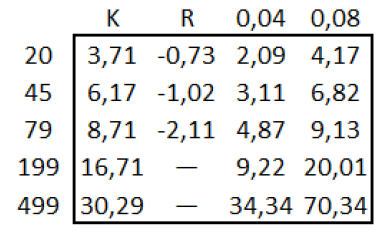
\includegraphics[width=0.42\textwidth]{poso-04.png}
% \par % так!!
% \caption{The main results of the computational experiments.}
% \mbox{\footnotesize Рис.~\arabic{ris-obho}. Об <<опоясывающем>> алгоритме.}
\label{table-1}
\end{table}

We think, that
the obtained results of computational experiments 
in general approximately correspond to the expected values.

\medskip

\textit{Acknowledgement.}
The work of the first author 
was partially supported by a grant 
from the scientific program of Chinese universities
``Higher Education Stability Support Program''
(section ``Shenzhen 2022~-- Science, Technology 
and Innovation Commission of Shenzhen Municipality'').

%
% ---- Bibliography ----
%
\begin{thebibliography}{5}

\bibitem{gu-pu}
Gutin, G., Punnen, A. (Eds.):
The traveling salesman problem and its variations.
Netherlands, Dordrecht: Kluwer Academic Publishers, 2002, 856~p.

\bibitem{KIO-2021}
Melnikov, B., Melnikova, E.
About the classical version of the branch and bound method.
Computer tools in education. 
2021. No.~1. Pp.~21-44 (in Russian).

\bibitem{KIO-2022}
Melnikov, B., Melnikova, E.
On the classical version of the branch and bound method.
Computer tools in education. 
2022. No.~2. Pp.~41-58.

\bibitem{Vasil-2022-1}
Melnikov, B.
On the object-oriented implementation
of the branch and bound method 
for the traveling salesman problem. Part I.
Modern information technologies and IT education. 
2022. Vol.~18. No.~2. Pp.~287-299 (in Russian).

\bibitem{Vasil-2022-2}
Melnikov, B.
On the object-oriented implementation
of the branch and bound method 
for the traveling salesman problem. Part II.
Modern information technologies and IT education. 
2022. Vol.~18. No.~3. Pp.~644-654 (in Russian).

\bibitem{SOI-2013}
Makarkin, S., Melnikov, B.
Geometric methods for solving the pseudo-geometric version 
of the traveling salesman problem.
Stochastic optimization in computer science. 
2013. Vol.~9. No.~2. Pp.~54-72 (in Russian).
\end{thebibliography}

%\end{document}  
\end{englisharticle}

\begin{englishtitle} % Настраивает LaTeX на использование английского языка
% Этот титульный лист верстается аналогично.
\title{Control of autonomous vehicles on the basis of the observation of surrounding landscape}
% First author
\author{Alexander Miller 
  \and
  Boris Miller 
  \and
Alexey Popov 
  \and
  Karen Stepanyan 
}
\institute{IITP RAS, Moscow, Russia\\
\email{amiller@iitp.ru,bmiller@iitp.ru,ap@iitp.ru,KVStepanyan@iitp.ru}
}
% etc

\maketitle

\begin{abstract}
Navigation based on observations of the current video image is one of the most promising means of navigation and control of unmanned vehicles in conditions of limited use of satellite navigation tools. 
In autonomous motion mode, simply adding a video camera in the absence of recognition and interpretation tools to the inertial navigation system does not have a significant effect. In this case the optical flow remains one of the main navigation tools.%~\cite{LucasKanade}.
Therefore, extracting navigation information from a sequence of images plays a key role. An important characteristic of the observed images is the evolution
generated information flow. Examples are optical flow during video surveillance, Doppler measurement of absolute velocity, and the evolution of the relief of the measured range using multipath sonars. From an algorithmic point
of view, they are very close, which allows us to combine their discussion in this report.

\keywords{unmanned vehicles, navigation, optical flow, estimation}
\end{abstract}

\end{englishtitle}

\iffalse
\documentclass[12pt]{llncs}  

% При использовании pdfLaTeX добавляется стандартный набор русификации babel.

\usepackage{iftex}

\ifPDFTeX
\usepackage[T2A]{fontenc}
\usepackage[utf8]{inputenc} % Кодировка utf-8, cp1251 и т.д.
\usepackage[english,russian]{babel}
\fi

\usepackage{todonotes} 

\usepackage[russian]{nla}

\begin{document}
\fi

\title{Управление автономными подвижными средствами на основе наблюдений за окружающим ландшафтом}
% Первый автор
\author{А.~Б.~Миллер 
  \and  
% Второй автор
  Б.~М.~Миллер 
  \and
% Третий автор
  А.~К.~Попов 
  \and
% Четвертый автор
  К.~В.~Степанян 
}

% Аффилиации пишутся в следующей форме, соединяя каждый институт при помощи \and.
\institute{Федеральное государственное бюджетное учреждение науки Институт проблем передачи информации им. А.А. Харкевича Российской академии наук (ИППИ РАН), Москва, Россия \\
  \email{amiller@iitp.ru,bmiller@iitp.ru,ap@iitp.ru,KVStepanyan@iitp.ru}
}

\maketitle

\begin{abstract}
Навигация по наблюдениям текущего видеоизображения является одним из наиболее перспективных средств навигации и управления беспилотными аппаратами в условиях ограниченного применения спутниковых средств навигации. В режиме автономного движения простое добавление видеокамеры при отсутствии средств распознавания и интерпретации к системе инерциальной навигации не дает значимого эффекта. Поэтому извлечение навигационной информации из последовательности изображений играет ключевую роль. Важной характеристикой наблюдаемых изображений является эволюция порождаемого информационного потока. Примерами являются оптический поток при видеонаблюдении, доплеровское измерение абсолютной скорости и эволюция рельефа измеренной дальности при использовании многолучевых сонаров. С алгоритмической точки
зрения они весьма близки, что позволяет объединить их обсуждение в данном докладе.

\keywords{беспилотный аппарат, навигация, оптический поток, оценивание} % в конце списка точка не ставится
\end{abstract}

\section*{Структура доклада}
\begin{enumerate}
\item
Управление БПЛА на основе пеленгационных измерений
\begin{itemize}
\item Геометрия оптико-электронной системы наблюдения. Модель камеры-обскуры\\ ({\it{pinhole camera}})
\item Угловые преобразования
\item Координатные преобразования
\item Модель пеленгационных измерений
\item Задачи и методы оценивания
\item Модифицированный метод псевдоизмерений
\end{itemize}
\item Управление БПЛА на основе видеопоследовательностей.
\begin{itemize}
\item Видеопоследовательность и оптический поток
\item Методы расчета оптического потока
\item Связь оптического потока с положением и движением БПЛА \item Примеры использования оптического потока
\end{itemize}
\item Заключение и выводы
\end{enumerate} 

\noindent {\bf Задачи и методы оценивания}
\begin{itemize}\item Разведка и целеуказание
\item Навигация БПЛА
\item Слежение за подвижными целями и определение их скоростей
\end{itemize}

\noindent {\bf Особенности задачи оценивания, различные методы}
\begin{itemize}
\item Линеаризованный и расширенный фильтр Калмана
\item Particle filter
\item Метод псевдоизмерений
\item Условно-оптимальный фильтр В. С. Пугачева
\end{itemize}

\noindent {\bf Комплексирование пеленгационных измерений со стандартными системами ИНС требует:}
\begin{itemize}
\item Несмещенности оценок
\item Знание их качества (средне-квадратических ошибок оценивания)
\item Учета случайности средне-квадратических характеристик ошибок оценивания
\end{itemize}





%\end{document}




\begin{englishtitle} % Настраивает LaTeX на использование английского языка
% Этот титульный лист верстается аналогично.
\title{An optimization approach to search of Nash equilibrium in nonmonotone quadratic games}
% First author
\author{Ilya Minarchenko}
\institute{Melentiev Energy Systems Institute SB RAS, Irkutsk, Russia\\
  \email{minar@isem.irk.ru}
}

\maketitle

\begin{abstract}
We investigate normal form game with quadratic payoffs and polyhedral strategy sets. The game is not supposed to be monotone and concave, therefore Nash equilibrium may not exist. The Nash equilibrium problem is reduced to minimization of nonconvex implicit function. Global and local search methods based on nonlinear support functions are proposed for this statement.

\keywords{Nash equilibrium, nonmonotone game, global optimization} % в конце списка точка не ставится
\end{abstract}
\end{englishtitle}

\iffalse
%%%%%%%%%%%%%%%%%%%%%%%%%%%%%%%%%%%%%%%%%%%%%%%%%%%%%%%%%%%%%%%%%%%%%%%%
%
%  This is the template file for the 6th International conference
%  NONLINEAR ANALYSIS AND EXTREMAL PROBLEMS
%  June 25-30, 2018
%  Irkutsk, Russia
%
%%%%%%%%%%%%%%%%%%%%%%%%%%%%%%%%%%%%%%%%%%%%%%%%%%%%%%%%%%%%%%%%%%%%%%%%


\documentclass[12pt]{llncs}

% При использовании pdfLaTeX добавляется стандартный набор русификации babel.

\usepackage{iftex}

\ifPDFTeX
\usepackage[T2A]{fontenc}
\usepackage[utf8]{inputenc} % Кодировка utf-8, cp1251 и т.д.
\usepackage[english,russian]{babel}
\fi

\usepackage{todonotes}

\usepackage[russian]{nla}

\begin{document}
\fi

\title{Оптимизационный подход к поиску равновесия\\ по Нэшу в немонотонных квадратичных играх}
% Первый автор
\author{И.~М.~Минарченко}

% Аффилиации пишутся в следующей форме, соединяя каждый институт при помощи \and.
\institute{Институт систем энергетики им. Л. А. Мелентьева СО РАН (ИСЭМ СО РАН), Иркутск, Россия \\
  \email{minar@isem.irk.ru}
}

\maketitle

\begin{abstract}
Исследуется игра в нормальной форме с квадратичными функциями выигрыша и множествами стратегий, заданными выпуклыми многогранниками. Монотонность и вогнутость игры не предполагается, в силу чего не гарантируется существование равновесия по Нэшу. Задача поиска равновесия сводится к задаче минимизации невыпуклой неявно заданной функции. Для решения указанной оптимизационной постановки предлагаются методы глобального и локального поиска, основанные на использовании нелинейных опорных функций.

\keywords{равновесие по Нэшу, немонотонная игра, глобальная оптимизация} % в конце списка точка не ставится
\end{abstract}

Рассмотрим игру $n$ лиц в нормальной форме. Пусть $N=\{ 1,2,\dots, n\}$ --- множество игроков, $X_i\subset \mathbb{R}^{m_i}$ --- множество стратегий $i$-го игрока, $m=m_1+m_2+\dots+m_n$ --- общее число переменных, $X=X_1\times X_2 \times \dots \times X_n\subset\mathbb{R}^m$ --- множество ситуаций игры, $f_i\colon X\rightarrow \mathbb{R}$ --- функция выигрыша $i$-го игрока. $\mathbb{R}$ обозначает множество действительных чисел. Для любого $i\in N$ будем предполагать, что $X_i$ является ограниченным множеством вида
\begin{equation*}
	\label{minar:X}
	X_i = \{ x_i\in \mathbb{R}^{m_i} \colon A_i x_i \leq b_i \},
\end{equation*}
где $A_i\in \mathbb{R}^{r_i\times m_i}$, $b_i\in \mathbb{R}^{r_i}$, $i\in N$. Функции выигрыша определим следующим образом:
\begin{equation*}
	\label{minar:f}
	f_i(x) = x_i^\top \left( \frac{1}{2}B_i x_i + d_i \right) + \sum_{j\in N\setminus\{i\}} x_i^\top C_{ij} x_j, \qquad i\in N,
\end{equation*}
где $B_i\in \mathbb{R}^{m_i\times m_i}$ --- симметричные и, вообще говоря, знаконеопределённые матрицы, $C_{ij} \in \mathbb{R}^{m_i\times m_j}$, $d_i\in \mathbb{R}^{m_i}$. Обозначим $(y_i,x_{-i}) = (x_1,x_2,\dots,x_{i-1},y_i,x_{i+1}, \dots, x_n)$. Задача заключается в нахождении равновесия по Нэшу, то есть такой ситуации $x^\ast\in X$, для которой выполнено
\begin{equation*}
	f_i(x_i^\ast, x_{-i}^\ast) \geq f_i(x_i, x_{-i}^\ast), \qquad x_i\in X_i, \quad i\in N.
\end{equation*}
Рассмотрим следующие функции~\cite{NikaidoIsoda1955}:
\begin{equation*}
	\varphi(x,y) = \sum_{i\in N} \left( f_i(y_i,x_{-i}) - f_i(x_i,x_{-i}) \right),\qquad
	F(x) = \max_{y\in X} \varphi(x,y).
\end{equation*}
Нетрудно убедиться, что $F(x)\geq 0$ для любых $x\in X$. Для того чтобы ситуация $x^\ast\in X$ являлась равновесием по Нэшу, необходимо и достаточно, чтобы $F(x^\ast) = 0$~\cite{NikaidoIsoda1955}. Отсюда следует, что множество равновесий является пустым тогда и только тогда, когда $F(x)>0$ для любых $x\in X$. Учитывая неотрицательность функции~$F$, рассмотрим задачу
\begin{equation}
	\label{minar:main_problem}
	F(x)\rightarrow\min, \qquad x\in X.
\end{equation}
Если множество равновесий непусто, то оно совпадает с множеством решений задачи~\eqref{minar:main_problem}~\cite{Khamisov2003}. Введём следующие векторы и матрицы:
$d =
  \begin{pmatrix}
  	d_1 & d_2 & \dots & d_n
  \end{pmatrix}^\top
$, %
$b =
  \begin{pmatrix}
  	b_1 & b_2 & \dots & b_n
  \end{pmatrix}^\top
$,
\begin{equation*}
  C =
  \begin{pmatrix}
    0 & C_{12} & \dots & C_{1n} \\
    C_{21} & 0 & \dots & C_{2n} \\
    \vdots & \vdots & \ddots & \vdots \\
    C_{n1} & C_{n2} & \dots & 0
  \end{pmatrix}
  ,\quad
  B =
  \begin{pmatrix}
    B_{1} & 0 & \dots & 0 \\
    0 & B_{2} & \dots & 0 \\
    \vdots & \vdots & \ddots & \vdots \\
    0 & 0 & \dots & B_{n}
  \end{pmatrix}
  ,\quad
  A =
  \begin{pmatrix}
    A_{1} & 0 & \dots & 0 \\
    0 & A_{2} & \dots & 0 \\
    \vdots & \vdots & \ddots & \vdots \\
    0 & 0 & \dots & A_{n}
  \end{pmatrix}
  .
\end{equation*}
Тогда для квадратичной игры функция~$F$ примет вид
\begin{equation*}
	F(x) = \max_{y\in X} \bigg[\frac{1}{2} y^\top By + y^\top (Cx+d) \bigg] - x^\top \left( \frac{1}{2}B+C \right) x - x^\top d,
\end{equation*}
где	$X = \{x \in \mathbb{R}^{m} \colon A x \leq b \}$. Для поиска глобального оптимума задачи~\eqref{minar:main_problem} предлагается метод, основанный на аппроксимации целевой функции снизу нелинейными опорными функциями. Если дополнительно предположить, что функции выигрыша строго вогнуты по собственным переменным, т.~е. матрицы $B_1, \dots, B_n$ отрицательно определены, то может быть рассмотрен метод локального поиска, основанный на d.c.-разложении функции~$F$.

% Рисунки и таблицы оформляются по стандарту класса article. Например,

%\begin{figure}[htb]
%  \centering
%  % Поддерживаются два формата:
%  %\includegraphics[width=0.7\linewidth]{figure.pdf} % Растровый формат
%  %\includegraphics[width=0.7\linewidth]{figure.png} % Векторный и растровый формат
%  %
%
%  \begin{center}
%    \missingfigure[figwidth=0.7\linewidth]{Уберите меня из статьи!}
%  \end{center}
%  \caption{Заголовок рисунка}\label{fig:example}
%\end{figure}



\begin{thebibliography}{9} % или {99}, если ссылок больше десяти.
\bibitem{NikaidoIsoda1955} Nikaido~H., Isoda~K. Note on non-cooperative convex games~// Pacific~J.~Math. 1955. Vol.~5. No.~5. Pp.~807--815.

\bibitem{Khamisov2003} Khamisov~O. A global optimization approach to solving equilibrium programming problems~// Optimization and Optimal Control. World Scientific, 2003. Pp.~155--164.

%Гантмахер~Ф.Р. Теория матриц. М.:~Наука,~1966.

%\bibitem{Kholl} Современные численные методы решения обыкновенных дифференциальных уравнений~/ Под~ред.~Дж.~Холл, Дж.~Уатт. М.:~Мир,~1979.

%\bibitem{Aleksandrov1} Александров~А.Ю. Об устойчивости сложных систем в критических случаях~// Автоматика и телемеханика. 2001. \textnumero~9. С.~3--13.

%\bibitem{Moreau1977} Moreau~J.-J. Evolution problem associated with a moving convex set in a Hilbert space~// J.~Differential~Eq. 1977. Vol.~26. Pp.~347--374.

%\bibitem{Semenov} Семенов~А.А. Замечание о вычислительной сложности известных предположительно односторонних функций~// Тр.~XII Байкальской междунар. конф. <<Методы оптимизации и их приложения>>. Иркутск, 2001. С.~142--146.

\end{thebibliography}

% После библиографического списка в русскоязычных статьях необходимо оформить
% англоязычный заголовок.




%\end{document}



\begin{englisharticle}


\iffalse
\documentclass[12pt]{llncs}

% The correcting style file is added.
\usepackage{todonotes}

\usepackage{nla} % This package is needed for compiling
                 % this template, it should be removed
                 % from your article.

% Many popular packages (amsXXX, graphicx, etc.) are already imported in the style file.
% If there is a conflict with your packages, try disabling them and compile
% the text.
%
% It would be convenient in the layout of the proceedings if the file names
% of the figures of different authors do not clash.
% To minimize the clash, the drawings can be placed in a separate subfolder
% named after the author or the title of the paper.
%
% \graphicspath{{ivanov-petrov-pics/}} % specifies the folder with images in png, pdf formats.
% or
% \graphicspath{{great-problem-solving-paper-pics/}}.

\begin{document}
\fi
% Text should be formatted in accordance with the 'article' class, using extensions like
% AMS.
%
\title{The problem of the inflow of a hot thermoviscous liquid into a cooled annular channel\thanks{The research work was supported by the state budget funds for the state assignment 124030400064-2 (FMRS-2024-0001).}}

% First author
\author{Mukhutdinova Aygul Ayratovna
}
\institute{Mavlyutov Institute of Mechanics UFRC RAS, Ufa, Russia\\
  \email{mukhutdinova23@ya.ru}}
% etc

\maketitle

\begin{abstract}
The features of the flow of a liquid, the viscosity of which depends on temperature, are studied under various conditions of heat exchange in an annular channel filled with a stationary liquid. The mathematical model includes the Navier-Stokes equations taking into account variable viscosity, as well as continuity and energy conservation equations. The influence of rheological parameters of the liquid and heat exchange conditions on the characteristics of liquid inflow has been established. It is shown that the hydrodynamic parameters of the flow strongly depend on the location of the flow region with high viscosity. Diagrams of axial velocity were constructed in various sections of the channel. The influence of channel geometry on the asymmetry of the temperature distribution and the viscous barrier was also noted.

\keywords{thermoviscous liquid, annular channel, heat-transfer conditions}
\end{abstract}

% at the end of the list, there should be no final dot
\section{The main results}

The processes of heat exchange between a fluid flow and the external environment largely determine the characteristics of the flow. In this case, taking into account the dependence of viscosity and thermophysical constants on temperature makes a significant contribution not only to the quantitative, but also to the qualitative characteristics of the flow. Under the assumption of an exponentially decreasing dependence of viscosity on temperature \cite{ref1}, a significant number of hydrodynamic studies have been carried out to solve various problems in geophysics, ecology, metallurgy and the chemical industry. Meanwhile, the dependence of viscosity on temperature can also have a non-monotonic character, the physical nature of which can be explained by the continuous processes of polymerization and decomposition of polymer chains. The nonmonotonic nature of the temperature dependence is revealed when determining the viscosity of some amorphous metal alloys in the liquid state \cite{ref2,ref3}. As was shown in \cite{ref4,ref5}, the property of non-monotonicity can be used in flow diverter technologies for the production of liquid hydrocarbons. The article \cite{ref6,ref7} presented results on determining the characteristics of the steady-state flow of an anomalously thermoviscous fluid in flat and annular channels.

In this work, a detailed study of the features of the inflow of liquid with a dependence of viscosity on temperature at various values of heat transfer parameters into a channel of an annular cross-section filled with a stationary liquid was carried out.

The mathematical model consists of modified Navier-Stokes equations taking into account variable viscosity, continuity and energy conservation equations, written in a cylindrical coordinate system in the presence of axial symmetry \cite{ref8}. The equations of the mathematical model are implemented using computer code based on the control volume method using the SIMPLE algorithm.

Using numerical modeling, the influence of rheological parameters of the liquid and heat exchange conditions on the characteristics of liquid inflow was established. It is shown that the hydrodynamic parameters of the flow strongly depend on the location of the flow region with high viscosity. Diagrams of axial velocity were constructed in various sections of the channel. The influence of channel geometry on the asymmetry of the temperature distribution and the viscous barrier was also noted.


\begin{thebibliography}{99} % or {99}, if there is more than ten references.

\bibitem{ref1} Vinogradov G.V., Malkin A.Ya. Rheology of Polymers. Moscow: Chemistry, 1977. 438 p. (Translation)

\bibitem{ref2} Tabachnikova E.D., Bengus V.Z., Egorov D.V., Tsepelev V.S., Ocelik V. Mechanical properties of amorphous alloys ribbons prepared by rapid quenching of the melt after different thermal treatments before quenching // Mater. Sci. Eng. A, 1997. Vol. 226--228. Pp. 887--890.

\bibitem{ref3} Ladyanov B.I., Beltyukov A.L., Shishmarnn A.I. Temperature and concentration dependences of viscosity of melts of the Fe-B system // Rasplavy (Melts). 2005. No. 4. Pp. 34--40. (Translation)

\bibitem{ref4} Altunina L.K., Kuvshinov V.A., Kuvshinov I.V., Stasyeva L.A., Chertenkov M.V., Andreev D.V., Karmanov A.Yu. Increasing oil recovery of the Permian-Carboniferous reservoir of high-viscosity oil of the Usinsk field by physicochemical and complex technologies (review) // Journal of SFU. Chemistry. 2018. Vol. 11. No. 3. Pp. 462--476. (Translation)

\bibitem{ref5} Toma A., Sayuk B., Abirov Zh., Mazbayev E. Polymer flooding for enhanced oil recovery in light and heavy oil fields // Territoriya Neftegaz. 2017. Pp. 58--67. (Translation)

\bibitem{ref6} Urmancheev S.F., Kireev V.N. Steady-state flow of a liquid with a temperature anomaly of viscosity // Reports of the Russian Academy of Sciences. 2004. Vol. 396. No. 2. P. 204--207. 

\bibitem{ref7} Kireev V.N., Mukhutdinova A.A., Urmancheev S.F. Towards heat transfer critical conditions for flow of fluids with a nonmonotonic dependence of viscosity on the temperature in annular channel // Fluid Dynamics, 2023, Vol. 58, No. 7, pp. 1310--1317.

\bibitem{ref8} Mukhutdinova A.A., Kireev V.N., Urmancheev S.F. Influence of variable thermophysical properties on the flow of fluids in an annular channel under intensive heat exchange // St Petersburg State Polytechnical University Journal. Physics and Mathematics. 2023. Vol. 16. No 1.1. Pp. 269--274.

\end{thebibliography}

%\end{document}

%%% Local Variables:
%%% mode: latex
%%% TeX-master: t
%%% End:

\end{englisharticle}

\begin{englishtitle} % Настраивает LaTeX на использование английского языка
% Этот титульный лист верстается аналогично.
\title{Decomposition of Webullah function into an orthogonal row}
% First author
\author{R.~R.~Mutigullina\inst{1}  \and  R.~D.~Murtazina\inst{2}
 }
\institute{UUST, Ufa, Russia\\
  \email{Regina.mutigullina@mail.ru}
  \and
  UUST, Ufa, Russia \\
\email{reginaufa@yandex.ru}
  }
% etc

\maketitle

\begin{abstract}
When expanding the Weibull distribution function into an orthogonal series of exponentials, the coefficients are uniformly convergent integrals with the parameter.

\keywords{Weibull function, orthogonal series, uniform convergence} % в конце списка точка не ставится
\end{abstract}
\end{englishtitle}


\iffalse
%%%%%%%%%%%%%%%%%%%%%%%%%%%%%%%%%%%%%%%%%%%%%%%%%%%%%%%%%%%%%%%%%%%%%%%%
%
%  This is the template file for the 6th International conference
%  NONLINEAR ANALYSIS AND EXTREMAL PROBLEMS
%  June 25-30, 2018
%  Irkutsk, Russia
%
%%%%%%%%%%%%%%%%%%%%%%%%%%%%%%%%%%%%%%%%%%%%%%%%%%%%%%%%%%%%%%%%%%%%%%%%

\documentclass[12pt]{llncs}  

% При использовании pdfLaTeX добавляется стандартный набор русификации babel.

\usepackage{iftex}

\ifPDFTeX
\usepackage[T2A]{fontenc}
\usepackage[utf8]{inputenc} % Кодировка utf-8, cp1251 и т.д.
\usepackage[english,russian]{babel}
\fi

\usepackage{todonotes} 

\usepackage[russian]{nla}

\begin{document}
\fi

\title{Разложение функции Вейбулла в ортогональный ряд}
% Первый автор
\author{Р.~Р.~Мутигуллина\inst{1}  \and Р.~Д.~Муртазина\inst{2}
 } % обязательное поле

% Аффилиации пишутся в следующей форме, соединяя каждый институт при помощи \and.
\institute{УУНиТ, Уфа, Россия \\
  \email{Regina.mutigullina@mail.ru}
  \and
  УУНиТ, Уфа, Россия \\
\email{reginaufa@yandex.ru}
  % \and Другие авторы...
}

\maketitle

\begin{abstract}
При разложении функции распределения Вейбулла в ортогональный ряд экспонент коэффициенты представляют собой равномерно сходящиеся интегралы с параметром.

\keywords{функция Вейбулла, ортогональный ряд, равномерная сходимость} % в конце списка точка не ставится
\end{abstract}

%\section{Основные результаты} % не обязательное поле

Рассмотрим функцию распределения Вейбулла
$$
f(t)=\frac{k}{r}\left(\frac{t}{r}\right)^{k-1}\cdot e^{-\left(\frac{t}{r}\right)^k},
$$
с параметрами $r=1$, $k=1,5$.


В работе получено разложение данной функции в ортогональный ряд
$$
f(t)=\sum_{l=1}^q a_l\phi_l(t),
$$ 
где ортогональные функции $\phi_l(t)$ выражаются в виде
$$
\phi_l(t)=\sum_{i=1}^l\lambda_{li}\cdot e^{-(i-1)\beta t},\quad l=1,2,\ldots.
$$ 

Будем считать, что $\beta=1$.
Коэффициенты $a_l$ ряда определяются так
$$
a_l=\int_0^{\infty}e^{-t}f(t)\phi_l(t)dt,
$$
а именно
$$
a_l=\frac{3}{2}\sum_{i=1}^l\lambda_{li}\int_0^{\infty}\sqrt{t}e^{-t\sqrt{t}-it}dt.
$$

Интеграл $\int_0^{\infty}\sqrt{t}e^{-t\sqrt{t}-it}dt$ равномерно сходится. Задавая границы интегрирования от $0$ до $5$ вычислим интегралы при $i=1,2,3,4,5,6$ методом прямоугольников, методом трапеций и методом Симпсона.
% В конце текста можно выразить благодарности, если этого не было
% сделано в ссылке с заголовка статьи, например,
%Работа выполнена при поддержке РФФИ (РНФ, другие фонды), проект \textnumero~00-00-00000.
%

\begin{thebibliography}{9} % или {99}, если ссылок больше десяти.
\bibitem{Ilin} Ильин~В.~А. Необходимые и достаточные условия базисности в $L^p$ и равносходимости с тригонометрическим рядом спектральных разложений по системе экспонент // Докл. АН СССР, 1983. Том~273. \textnumero~4. С.~789--793.

\bibitem{Xabib} Хабибуллин~Б.~Н. Полнота систем экспонент и множества единственности.  Уфа:~ РИЦ БашГУ, 2011.


\bibitem{KrTer}	Красичков-Терновский~И.Ф., Шилова~Г.Н. Абсолютная полнота систем экспонент на выпуклых компактах // Матем. сб., 2005. V.~196. \textnumero~12. С.~85--98.

\bibitem{Leo}	Леонтьев~А.Ф. О полноте системы экспонент на кривой // Сиб. матем. журнал, 1974. Т.~15. \textnumero~5. С.~1103--1114.

\bibitem{Leo2}	Леонтьев~А.Ф. Ряды экспонент. М.:~Наука, 1976.
\end{thebibliography}
% После библиографического списка в русскоязычных статьях необходимо оформить
% англоязычный заголовок.




%\end{document}


\begin{englishtitle} % Настраивает LaTeX на использование английского языка
% Этот титульный лист верстается аналогично.
\title{On calculating the mapping degree of the gradient of a smooth positively homogeneous function}
% First author
\author{Alizhon Naimov  \and  Alexander Korovin 
}
\institute{Vologda State University, Vologda, Russia\\
 \email{naimovan@vogu35.ru ,   korovinal@vogu35.ru}
 }  

\maketitle

\begin{abstract}
The report addresses the issue of calculating the mapping degree of the gradient of a smooth positively homogeneous function on the unit sphere of the Euclidean space $\mathrm{R}^n$, $n\geq 2$. A scheme for proving the formula for calculating rotation is discussed and some consequences are given. The formula for calculating the mapping degree is refined in cases where the set of zeros of a function has a certain structure or
  a function is represented by a product of simpler functions.

\keywords{positively homogeneous function, gradient of a function, 
vector field,  mapping degree of a vector field (topological degree), 
Euler characteristic} % в конце списка точка не ставится
\end{abstract}
\end{englishtitle}

\iffalse
\documentclass[12pt]{llncs}

% При использовании pdfLaTeX добавляется стандартный набор русификации babel.

\usepackage{iftex}

\ifPDFTeX
\usepackage[T2A]{fontenc}
\usepackage[utf8]{inputenc} % Кодировка utf-8, cp1251 и т.д.
\usepackage[english,russian]{babel}
\fi

\usepackage{todonotes}

\usepackage[russian]{nla}

\begin{document}
\fi
% Текст оформляется в соответствии с классом article, используя дополнения
% AMS.
%

\title{О вычислении вращения градиента гладкой положительно однородной функции\thanks{Исследование выполнено за счет гранта
Российского научного фонда \textnumero 23-21-00032, https://rscf.ru/project/23-21-00032/}}
% Первый автор
\author{А.~Н.~Наимов \and А.~Л.~Коровин
 } % обязательное поле

% Аффилиации пишутся в следующей форме, соединяя каждый институт при помощи \and.
\institute{Вологодский государственный университет (ВоГУ), Вологда, Россия\\
  \email{naimovan@vogu35.ru,  korovinal@vogu35.ru}
 % \and Другие авторы...
}

\maketitle

\begin{abstract}
В докладе рассматривается вопрос о вычислении вращения (степени отображения) градиента гладкой положительно однородной функции на единичной сфере евклидового  пространства $\mathrm{R}^n$, $n\geq 2$. 
Обсуждается схема доказательства формулы вычисления вращения и приводятся некоторые следствия.
Формула вычисления вращения уточняется в случаях, когда множество нулей функции имеет определенную структуру или
 функция представлена произведением более простых функций.
 
\keywords{положительно однородная функция,
 градиент функции, векторное поле, вращение векторного поля,
 эйлерова характеристика} % в конце списка точка не ставится
\end{abstract}


Вычисление вращения (степени отображения) векторных полей представляет интерес в приложении методов нелинейного функционального анализа 
в теории дифференциальных и интегральных уравнений. Можно отметить работы \cite{K66},  \cite{KZ75}, \cite{M96}, где методы вычисления 
вращения векторных полей применяются к исследованию существования 
периодических и ограниченных решений систем нелинейных 
обыкновенных дифференциальных уравнений. 

В работе \cite{M96} анонсирована формула 
\begin{equation}\label{for1}
\gamma(\nabla v, S^{n-1})=1-\chi (\overline{\Omega}_-(v)),
\end{equation}
где $\gamma(\nabla v, S^{n-1})$ -- вращение градиента $\nabla v$
гладкой положительно однородной функции 
$v\in C^1(\mathrm{R}^n\setminus\{0\};\mathrm{R}^1)$, 
$\nabla v(x)\neq 0$ $\forall x\in S^{n-1}$, 
на единичной сфере $S^{n-1}=\{x\in \mathrm{R}^n : |x|=1 \}$ 
евклидового пространства $\mathrm{R}^n$, $n\geq 2$,
 $\chi (\overline{\Omega}_-(v))$ -- эйлерова характеристика
замыкания множества
$$
\Omega_-(v)=\{x\in S^{n-1} : v(x)<0 \},
$$ 
при этом $\chi (\overline{\Omega}_-(v))=0$, если 
$\Omega_-(v)$ пусто. В работах \cite{MN21}, \cite{MN22},  используя формулу (\ref{for1}),  доказаны теоремы о существовании периодических и ограниченных  решений для систем обыкновенных дифференциальных уравнений первого порядка с главной градиентной положительно однородной нелинейностью.

В работе \cite[с. 3-4]{A78} дано пояснение, 
как формулы вида (\ref{for1}) можно получить 
непосредственным применением теории Морса. 
В настоящей работе предложена схема 
доказательства формулы (\ref{for1}). Суть предложенной схемы состоит в том, что вычисление  $\gamma(\nabla v, S^{n-1})$ 
сводится к вычислению вращений  касательной составляющей
$$
\nabla v(x)-\langle \nabla v(x) , x \rangle \frac{x}{|x|^2}, 
\quad x\in S^{n-1},
$$
 на границах связных компонент множества $\Omega_-(v)$, где 
$
\langle x , y \rangle = x_1y_1 + \ldots + x_ny_n
$
 --  скалярное произведение в $\mathrm{R}^n$.
Установлено, что вращение касательной составляющей на границе каждой 
связной компоненты равно эйлеровой характеристике замыкания
данной связной компоненты. 
 Схему доказательства  можно
применить для вычисления вращения неградиентных векторных полей (см., например, \cite{MN23}). 

Справедливы следующие уточнения формулы (\ref{for1}).

{\bf Теорема 1}. {\it Если множество
$
\Omega_0(v)=\{x\in S^{n-1} : v(x)=0 \}
$
состоит из $p_0(v)$ связных компонент, каждая из которых диффеоморфна сфере $S^{n-2}$, то верна формула
$$
\gamma(\nabla v, S^{n-1})=\left\{
\begin{array}{cl}
1-p_0(v), & \text{если n -- четно,}\\
p_+(v)-p_-(v), & \text{если n -- нечетно,}\\
\end{array}
\right.
$$
где $p_{\pm}(v)$ -- число связных компонент множества 
$\Omega_{\pm}(v)=\{x\in S^{n-1} : \pm v(x)>0 \}$.
}

Условие теоремы 1 при $n=3$  всегда выполняется. При $n=4$ 
  множество $\Omega_0(v)$ состоит из $p_0(v)$ двумерных
ориентируемых гладких многообразий без края. Каждое такое многообразие,
как известно, диффеоморфно сфере с ручками. Зная набор количества ручек
$r_1, \ldots , r_{p_0(v)}$ связных компонент, находим
$$
\chi(\Omega_0(v))=2(1-r_1) +  \ldots + 2(1- r_{p_0(v)}).
$$

{\bf Теорема 2}. {\it Если $n=4$, то верна формула
$$
\gamma(\nabla v, S^{3})=1 - p_0(v) + r_1  +  \ldots + r_{p_0(v)},
$$
где $r_1, \ldots , r_{p_0(v)}$ --  набор количества ручек связных компонент 
множества $\Omega_0(v)$.
}

{\bf Теорема 3}. {\it Пусть функции 
$v_i\in C^1(\mathrm{R}^n\setminus\{0\};\mathrm{R}^1)$, $i=\overline{1, N}$
удовлетворяют условиям

а) $\nabla v_i(x)\neq 0$ $\forall x\neq 0$, $i=\overline{1, N}$;

б) $|v_i(x)|+|v_j(x)|>0$  $\forall x\neq 0$, $i\neq j$;

в) $\forall  i=\overline{1, N-1}$ либо 
$\Omega_-(v_i)\subset \Omega_+( v_{i+1}\cdot \ldots \cdot v_N)$,
либо 
$\Omega_-(v_i)\subset \Omega_-( v_{i+1}\cdot \ldots \cdot v_N)$.

Тогда верна формула
$$
\chi(\overline{\Omega}_-(v_1\cdot \ldots \cdot v_N))=
\sum_{i=1}^{N-1}
\sigma(v_i; v_{i+1}\cdot \ldots \cdot v_N)
\chi(\overline{\Omega}_-(v_i)) +
\chi(\overline{\Omega}_-(v_N)),
$$
где
$$
\sigma(v_1; v_2)=\left\{
\begin{array}{cl}
1, & \text{если}\quad \Omega_-(v_1)\subset\Omega_+(v_2), \\
(-1)^n, & \text{если}\quad \Omega_-(v_1)\subset\Omega_-(v_2).\\
\end{array}
\right.
$$
В частности, 
$$
\chi(\overline{\Omega}_-(v_1\cdot \ldots \cdot v_N))=
\sum_{i=1}^{N}
\chi(\overline{\Omega}_-(v_i)), \qquad \text{если} \quad n - \text{четно}.
$$
}

Аналогично работе \cite[Lemma 2]{MN_IA21} можно показать, что любую положительно однородную (порядка $m>0$) функцию 
$v\in C^1(\mathrm{R}^n\setminus\{0\};\mathrm{R}^1)$,
градиент которой не обращается в ноль, можно представить в виде произведения 
$v(x)=|x|^{m-N}v_1(x)\cdot \ldots \cdot v_N(x)$, где $N=p_0(v)$,
функции $v_i$, $i=\overline{1, N}$ 
положительно однородные порядка 1 и
удовлетворяют условиям а) -- в), а соответствующие им множества $\Omega_0(v_i)$, 
$i=\overline{1, N}$ совпадают со связными компонентами $\Omega_0(v)$.

% Список литературы оформляется подобно ГОСТ-2008.
% Примеры оформления находятся по этому адресу -
%     https://narfu.ru/agtu/www.agtu.ru/fad08f5ab5ca9486942a52596ba6582elit.html
%


\begin{thebibliography}{9} % или {99}, если ссылок больше десяти.

\bibitem{K66}  Красносельский, М.А.   
{\it Оператор сдвига по траекториям дифференциальных уравнений}
/ М.А. Красносельский. --  М.: Наука, 1966. -- 330~с.

\bibitem{KZ75}  Красносельский, М.А., Забрейко, П.П.    
{\it Геометрические методы нелинейного анализа}
/ М.А. Красносельский, П.П. Забрейко. --  М.: Наука, 1975. -- 512~с.

\bibitem{M96} Мухамадиев, Э. {\it Ограниченные решения и гомотопические
инварианты систем  нелинейных дифференциальных уравнений} 
/ Э. Мухамадиев // Докл. РАН. -- 1996. -- Т.~351. №~5. -- С.~596-598.

\bibitem{MN21} Мухамадиев, Э., Наимов, А.Н. {\it Критерии существования периодических и ограниченных решений 
для трехмерных систем дифференциальных уравнений} 
/ Э. Мухамадиев, А.Н. Наимов // Тр. ИММ УрО РАН. -- 2021. -- Т.~27. №~1.
 -- С.~157–172.

\bibitem{MN22} Мухамадиев, Э., Наимов, А.Н. {\it Об априорной оценке 
и существовании периодических решений для одного класса 
систем нелинейных обыкновенных дифференциальных уравнений} 
/ Э. Мухамадиев, А.Н. Наимов // Изв. вузов. Матем. -- 2022. -- №~4.
 -- С.~37–48.

\bibitem{A78} Арнольд, В.И. {\it Индекс особой точки векторного поля, неравенства 
Петровского–Олейник и смешанные структуры Ходжа} 
/ В.И. Арнольд // Функц. анализ и его прил. -- 1978. -- Т.~12. №~1.
 -- С.~1–14.
 
\bibitem{MN23} Мухамадиев, Э., Наимов, А.Н. {\it К вопросу о вычислении 
вращения конечномерного векторного поля} 
/ Э. Мухамадиев, А.Н. Наимов // Изв. вузов. Матем. -- 2023. -- №~6.
 -- С.~67–73. 

\bibitem{MN_IA21} Mukhamadiev, E., Naimov, A.N. 
{\it On the homotopy classification of positively homogeneous 
functions of three variables} 
/ E. Mukhamadiev, A.N. Naimov // Issues Anal. -- 2021. -- V.~10. №~2.
 -- P.~67–78.

\end{thebibliography}

% После библиографического списка в русскоязычных статьях необходимо оформить
% англоязычный заголовок.




%\end{document}

\begin{englishtitle}
\title{Stabilization of linear three-dimensional stationary discrete systems}
% First author
\author{Vladislav O. Nesterov}
\institute{Adyghe State University, Maykop, Adyghe Republic, Russia\\
\email{v.nesterov@adygnet.ru}}
% etc

\maketitle

\begin{abstract}
The paper deals with the  problem of stabilisation of a three-dimensional linear stationary discrete system by nonstationary feedback. The solution of this problem lies in the context of solving the discrete analogue of the Brockett problem on stabilisation of multidimensional linear stationary discrete controlled systems by means of linear nonstationary feedback. We consider the cases when in the controlled system the output is one of the coordinates of the state vector.The nonstationary stabilising feedback is sought in the class of periodic feedbacks of period three.

\keywords{linear discrete system, stabilisation, asymptotic stability, periodic feedback, controlled and observed system, characteristic polynomial, stabilisation region, monodromy matrix}
\end{abstract}
\end{englishtitle}

\iffalse
\documentclass[12pt]{llncs}
\usepackage[T2A]{fontenc}
\usepackage[utf8]{inputenc}
\usepackage[english,russian]{babel}
\usepackage[russian]{nla}

%\usepackage[english,russian]{nla}

% \graphicspath{{pics/}} %Set the subfolder with figures (png, pdf).

%\usepackage{showframe}
\begin{document}
%\selectlanguage{russian}
\fi

\title{Стабилизация трехмерных линейных дискретных систем периодической обратной связью}
% Первый автор
\author{В.~О.~Нестеров%\inst{1}
%  \and
% Второй автор
%  И.~О.~Фамилия\inst{2}
%  \and
% Третий автор
%  И.~О.~Фамилия\inst{2}
} 
\institute{Факультет математики и компьютерных наук\\ Адыгейский государственный университет, Адыгея, Россия\\
  \email{v.nesterov@adygnet.ru}
  }


\maketitle

\begin{abstract}
В докладе рассматривается задача стабилизации трехмерной линейной стационарной дискретной системы нестационарной обратной связью. Решение данной задачи лежит в русле решения дискретного аналога проблемы Брокетта о стабилизации многомерных линейных стационарных дискретных управляемых систем с помощью линейной нестационарной обратной связи. Рассматриваются случаи, когда в управляемой системе выходом является одна из координат вектора состояния. Нестационарная стабилизирующая обратная связь ищется в классе периодических обратных связей периода три.

\keywords{линейная дискретная система, стабилизация, асимптотическая устойчивость, периодическая обратная связь, управляемая и наблюдаемая система, характеристический многочлен, область стабилизации, матрица монодромии}
\end{abstract}

%\section{Основные результаты} % не обязательное поле

В докладе рассматривается задача стабилизации трехмерной линейной стационарной дискретной системы нестационарной обратной связью \cite{vor1,vor2,vor3}. 
Построены нестационарные обратные связи  -- периодические с периодом 3, стабилизирующие рассматриваемую систему. Получены коэффициентные достаточные условия стабилизируемости рассматриваемой системы. В случае, когда выходом является первая или вторая координата вектора состояния, построенная нестационарная обратная связь расширяет в целом область стационарной стабилизации. В случае, когда выходом является третья координата вектора состояния, не происходит расширения области стацио-нарной стабилизации.


% Список литературы.
\begin{thebibliography}{99}
\bibitem{vor1}
Леонов Г. А. Проблема Брокетта для линейных дискретных систем управления~// Автоматика и телемеханика 2002. \textnumero~5. С.~92–96
\bibitem{vor2}
% Format for Journal Reference:
Леонов Г. А., Шумафов. М. М, Методы стабилизации линейных управляемых систем. СПб.: Изд-во С.-Петерб. ун-та, 2005. С.~420 с.
% Format for books:
\bibitem{vor3}
Шумафов М. М. К задаче стабилизации двумерной линейной дискретной системы~// Известия вузов. Северо-Кавказский регион. 2009.  \textnumero~5. С.~71–74.
% Format for Russian Journal Reference:.
% etc
\end{thebibliography}


% Обязательная информация на английском языке:




%\end{document}


\begin{englishtitle}
\title{The method of fictitious domains for an equilibrium problem of a Kirchhoff-Love plate with a flat rigid inclusion}
% First author
\author{N.~A.~Nikolaeva}
\institute{North Eastern Federal University, Yakutsk, Russia\\
  \email{niknataf@mail.ru}
 }
% etc

\maketitle

\begin{abstract}
An equilibrium problem for a plate with a flat rigid inclusion is considered. It is assumed that a flat rigid inclusion reaches the boundary at the zero angle and partially contacts a rigid body. The existence and uniqueness of a solution to the problem are proved.
We present differential and variational formulations of the problem. 

\keywords{plate, flat rigid inclusion, fictitious domain}
\end{abstract}
\end{englishtitle}



\iffalse
\documentclass[12pt]{llncs}
\usepackage[T2A]{fontenc}
\usepackage[utf8]{inputenc}
\usepackage[english,russian]{babel}
\usepackage[russian]{nla}

%\usepackage[english,russian]{nla}

% \graphicspath{{pics/}} %Set the subfolder with figures (png, pdf).

%\usepackage{showframe}
\begin{document}
%\selectlanguage{russian}
\fi

\title{Метод фиктивных областей в задаче о равновесии пластины Кирхгофа-Лява с плоским жестким включением\thanks{Работа выполнена при поддержке гранта РНФ, проект \textnumero~24-21-00081.}}
% Первый автор
\author{Н.~А.~Николаева
} % обязательное поле
\institute{Северо-Восточный федеральный университет им. М. К. Аммосова,
г. Якутск, Россия\\
  \email{niknataf@mail.ru}
  }
% Другие авторы...

\maketitle

\begin{abstract}
Исследуется задача о равновесии пластины, которая содержит плоское жесткое включение. Предполагается, что плоское жесткое включение выходит на границу под нулевым углом и частично контактирует с недеформируемым телом. Доказана теорема существования и единственности решения задачи. Приведены дифференциальная и вариационная формулировки задачи. 

\keywords{пластина, плоское жесткое включение, фиктивная
область}
\end{abstract}

%\section{Основные результаты} % не обязательное поле

%Текст доклада на русском языке.



% Список литературы.
\begin{thebibliography}{99}
\bibitem{1}
Khludnev A.\,M., Kovtunenko V.\,A., Analysis of cracks in solids.  Southampton New York: WIT-Press, 2000.
\bibitem{2}
% Format for Journal Reference:
Nikolaeva N. A., Kirchhoff--Love plate with a flat rigid inclusion. Chelyab. Fiz.-Mat. Zh. 2023. vol~8, No~1. Pp.~29-46.
\bibitem{3}
Nikolaeva N. A., Method of fictitious areas in a task about balance of a plate of Kirchhoff–Lyava. J. Math. Sci. 2017. Vol.~221, No~6.Pp. 872–882.

\end{thebibliography}


% Обязательная информация на английском языке:




%\end{document}




\begin{englishtitle}
\title{Numerical solution of a particular control problem with phase constraints}
% First author
\author{Dmitrii Novikov
%Name FamilyName2\inst{2}
}
\institute{Institute of Mathematics and Mechanics, Ural Branch of the Russian Academy of
	Sciences, Yekaterinburg, Russia\\
  \email{ya.novikovdmitry@imm.uran.ru}
%  \and
%Affiliation, City, Country\\
%\email{email}
}
% etc

\maketitle

\begin{abstract}
The problem of controlling the horizontal movement of a rod on a plane is considered. The rod is controlled by a constant modulo force applied to one of its ends. The rate of change of the angle between the rod and the vector specifying the direction of the specified force is used as a control parameter. Restrictions are imposed on the control and the current phase state of the dynamic system describing the movement of the rod. The desired control must satisfy the constraints and ensure that the rod is placed on a given vertical axis with zero velocity and with the required spatial orientation, with all restrictions on the current phase state of the dynamic system describing its movement being fulfilled. A particular method for constructing such a control is discussed, based on the decomposition of a linear system of differential equations in a mathematical model of the problem. Two auxiliary tasks are considered. The solution of the first forms a reference function of the angle determining the deviation of the rod from the vertical, the solution of the second determines the desired control. The results obtained are illustrated by examples of numerical solutions to a number of model problems.

\keywords{linear dynamic system, system decomposition, phase constraints, performance problem, optimal control}
\end{abstract}
\end{englishtitle}

\iffalse
\documentclass[12pt]{llncs}
\usepackage[T2A]{fontenc}
\usepackage[utf8]{inputenc}
\usepackage[english,russian]{babel}
\usepackage[russian]{nla}

\begin{document}
%\selectlanguage{russian}
\fi

\title{Численное решение задачи управления с фазовыми ограничениями}
% Первый автор
\author{Д.~А.~Новиков%\inst{1}
%  \and
% Второй автор
%  И.~О.~Фамилия\inst{2}
%  \and
% Третий автор
%  И.~О.~Фамилия\inst{2}
} % обязательное поле
\institute{Институт математики и механики УрО РАН (ИММ УрО РАН), Екатеринбург, Россия\\
  \email{ya.novikovdmitry@imm.uran.ru}
%  \and
%Институт (название в краткой форме), Город, Страна\\
%\email{email}
}
% Другие авторы...

\maketitle

\begin{abstract}
Рассматривается задача управления горизонтальным движением стержня на плоскости. Управление стержнем осуществляется с помощью постоянной по модулю силы, приложенной к одному из его концов, которая отклоняет стержень от вертикального положения. В качестве управляющего параметра используется скорость изменения угла между стержнем и вектором, задающим направление указанной силы. На управление и текущее фазовое состояние динамической системы, описывающей движение стержня, накладываются ограничения. Искомое управление должно удовлетворять ограничениям и обеспечивать выведение стержня на заданную вертикальную ось с нулевой скоростью и с требуемой пространственной ориентацией, с выполнением всех ограничений на текущее фазовое состояние динамической системы, описывающей его движение. Обсуждается один подход построения такого управления, основанный на декомпозиции линейной системы дифференциальных уравнений в математической модели задачи. Рассматриваются две вспомогательные задачи управления. Решение первой формирует эталонную функцию угла, определяющего отклонение стержня от вертикали. Решение второй на основе этой эталонной функции определяет искомое управление в исходной задаче. Полученные результаты иллюстрируются примерами численного решения ряда модельных задач. 

\keywords{линейная динамическая система, декомпозиция системы, фазовые ограничения, задача быстродействия, оптимальное управление}
\end{abstract}

\section{Постановка задачи} % не обязательное поле


Рассматривается линейная система дифференциальных уравнений, описывающая горизонтальное и вращательное движения стержня на плоскости:
\begin{equation}\label{eq:NovikovDA:20231002}
\begin{aligned}
	&\dot x=v \\
	&\dot{v}=-\frac{p}{m}\cdot (\vartheta+\delta) \\
	&\dot{\vartheta}=\omega \\
	&\dot{\omega}=-\frac{l}{J}\cdot p\cdot \delta \\
	&\dot \delta = u
\end{aligned},
\qquad t\in [0,t_f],
\end{equation}
где $x$~--~положение центра масс стержня, $v$~--~его скорость,  $\vartheta$~--~угол отклонения оси стержня от вертикали,  $\omega$~--~угловая скорость вращения стержня вокруг центра масс, $\delta$~--~угол между направлением приложенной силы и оси стержня, $m$~--~масса стержня, $p$~--~величина постоянной по модулю приложенной к концу стержня силы, $l$~--~длина стержня, $J$~--~его момент инерции стержня.

В момент времени $t=0$ для системы \eqref{eq:NovikovDA:20231002} заданы начальные условия: 
\begin{equation}\label{eq:NovikovDA:202310051}
	x=x_0 \qquad v=v_0 \qquad  \vartheta=\vartheta_0  \qquad\omega=\omega_0 \qquad \delta=\delta_0
\end{equation}

Значения $\vartheta$ и $\delta$ должны удовлетворять ограничениям:
\begin{equation}\label{eq:NovikovDA:202310021}	
	\begin{aligned}
		&|\vartheta| \leq \vartheta^{\max}\\
		&|\delta| \leq \delta^{\max} \\	
	\end{aligned}
\end{equation}

На управление $u$ накладывается ограничение:
\begin{equation}\label{eq:NovikovDA:202310022}
	\begin{aligned}
		&|u| \leq u^{\max}\\
	\end{aligned}
	\qquad t\in [0,t_f]
\end{equation}

Пусть начальный момент времени $t_f$ не зафиксирован, но считая его формально заданным, можно сформулировать следующую задачу управления.

З~а~д~а~ч~а~1. Для системы \eqref{eq:NovikovDA:20231002}, у которой в момент времени $t=0$ задано начальное условие \eqref{eq:NovikovDA:202310051}, требуется на интервале времени $[0,t_f]$ найти управление $u$ (кусочно-постоянную функцию), удовлетворяющее ограничению \eqref{eq:NovikovDA:202310022} и обеспечивающее перевод системы \eqref{eq:NovikovDA:20231002} из начального фазового состояния \eqref{eq:NovikovDA:202310051} в конечное состояние:
\begin{equation}\label{eq:NovikovDA:202310052}
	x^f=0\text{,} \qquad  {v}^f = 0\text{,} \qquad  \vartheta^f=0\text{,} \qquad  \omega^f=0\text{,} \qquad  \delta^f=0\text{.}
\end{equation}

% Требуется найти управление $u$ как кусочно-постоянную скалярную функцию, удовлетворяющую ограничению, обеспечивающую выполнение фазовых ограничений, и на некотором нефиксированном интервале времени $t \in [0,t_f]$  приводит центр масс стержня на вертикальную ось, задаваемую уравнением  $x=0$, с нулевой вертикальной составляющей скоростью ${\vx} = 0$. Дополнительно стержень в конечный момент должен иметь горизонтальное положение и нулевую угловую скорость, а также ее производную: 
%\begin{equation}\label{eq:NovikovDA:202310052}
%	x^f=0 \qquad  {\vx}^f = 0 \qquad  \vartheta^f=0 \qquad  \omega^f=0 \qquad  \delta^f=0
%\end{equation}
%Частным случаем задачи является отсутствия условия $x^f=0$, что приводит к задаче торможения.

\section{Основные результаты} % не обязательное поле

Для решения задачи~1 предлагается рассмотреть две вспомогательные задачи управления.

В первой рассматривается динамическая система, описывающая поступательное движение центра масс стержня, в предположении, что отклонение силы $p$ от оси стержня мало и отлично от нуля на небольшом интервале времени:
\begin{equation}\label{eq:NovikovDA:202310053}
	\begin{aligned}
		&\dot x=v \\
		&\dot{v}=-\frac{p}{m}\cdot \vartheta \\
	\end{aligned},
	\quad t \in [0,\tau_f].
\end{equation}
Для системы \eqref{eq:NovikovDA:202310053} задаются начальные
\begin{equation}\label{eq:NovikovDA:202310054}
x(0)=x_0,~~~v(0)= v_0
\end{equation}
и конечные 
\begin{equation}\label{eq:NovikovDA:202310055}
x(\tau_f)=0,~~~v(\tau_f)= 0
\end{equation}
условия. В качестве управления используется функция $\vartheta$, на значения которой накладывается ограничение 
\begin{equation}\label{eq:NovikovDA:202310056}
|\vartheta|\leq \vartheta^{\max}\qquad t\in[0,\tau_f]
\end{equation}

Для системы \eqref{eq:NovikovDA:202310053} решается задача быстродействия:
\begin{equation}\label{eq:NovikovDA:202310057}
J(\vartheta) = \int_{0}^{\tau_f} dt \to \min
\end{equation}
Эталонной функцией $\vartheta^*(t)$, $t\in[0,\tau^*_f]$ будем называть решение задачи~\eqref{eq:NovikovDA:202310057}.

Затем строится разбиение промежутка времени $[0,\tau^*_f]$
\begin{equation}
t_{k+1}=t_k+\Delta t\text{,~~где~~~~} t_0=0, \quad \Delta t=\frac{\tau_f}{N}
\end{equation}

Во второй вспомогательной задаче на каждом элементарном интервале $[t_k,t_{k+1}]$ рассматривается система
\begin{equation}\label{eq:NovikovDA:202403301}
\begin{aligned}
&\dot{\vartheta}=\omega \\
&\dot{\omega}=-\frac{l}{J}\cdot p\cdot \delta \\
&\dot \delta = u \text{,}\\
\end{aligned}, \quad t \in [t_k,t_{k+1}]
\end{equation} 
фазовое состояние которой в момент $t=t_0$ задается условиями \eqref{eq:NovikovDA:202310051}. Выполняется итерационная по элементарным интервалам времени процедура, на каждом шаге которой с помощью алгоритма, изложенного в \cite{1}, определяется управление $u^*_k(t)$, где $t\in[t_k,t_{k+1}]$. С помощью этого управления система \eqref{eq:NovikovDA:202403301} переводится из текущего состояния в заданное состояние:
\begin{equation}
\vartheta(t_{k+1})=\vartheta^*(t_{k+1})\text{,} \qquad   \omega(t_{k+1})=0\text{,} \qquad  \delta(t_{k+1})=0\text{.}
\end{equation}

В результате такой итерационной процедуре строится управление 
\begin{equation}
u^*(t)=	\left \{u^*_k(\tau), \tau\in[t_k,t_{k+1}] : k=1,\ldots N-1 \right \}\text{,}
\end{equation}
которое удовлетворяет ограничению \eqref{eq:NovikovDA:202310022} и переводит систему \eqref{eq:NovikovDA:20231002} из начального фазового состояния \eqref{eq:NovikovDA:202310051}  в состояние
\begin{equation}\label{eq:NovikovDA:202404141}
x(\tau^*_f)=0\text{,} \qquad  {v}(\tau^*_f) = 0\text{,} \qquad  \omega(\tau^*_f)=0\text{,} \qquad  \delta(\tau^*_f)=0\text{,}
\end{equation}
в котором $\vartheta(\tau^*_f) \neq 0$. 

Чтобы обеспечить выполнение условия \eqref{eq:NovikovDA:202310052}, на интервале времени $t\in[t_N,t_f]$ с помощью алгоритма, предложенным в \cite{1}, строится  управление $u^*_N$, которое переводит систему из фазового состояния \eqref{eq:NovikovDA:202404141} в конечное  состояние \eqref{eq:NovikovDA:202310052}.

Таким образом, искомое управление для исходной задачи примет вид

\begin{equation}
u^*(t)=	
\begin{cases}
u^*_k(t),& t\in[t_k,t_{k+1}) \\
u^*_N(t),& t\in[t_N,t_f] 
\end{cases}	
\end{equation}

Полученные результаты иллюстрируются двумя численными примерами.

% Список литературы.
\begin{thebibliography}{99}
\bibitem{1}
% Format for Journal Reference
Новиков~Д.А. {О простейшей задаче быстродействия с фазовым ограничением при управлении пространственной ориентацией тела} // Труды Института математики и механики УрО РАН. 2023. Т.~29, No~3. С.~62-72.
\bibitem{2}
% Format for Journal Reference
Новиков~Д.А.,~Кандоба И.Н.,~Козмин И.В.,~Плаксин А.Р. { О решении одной задачи управления движением объекта в плотных слоях атмосферы} // Труды Института математики и механики УрО РАН. 2021. Т.~27, No~2. С.~169-184.
\bibitem{3} Благодатских~В.И. { Введение в оптимальное управление (линейная теория)}. М.: Высш. шк., 2001.

\bibitem{4} Лебедев~А.А., Герасюта~Н.Ф. { Баллистика ракет}. М.: Машиностроение, 1970.

\bibitem{5} Васильев~Ф.П. { Методы оптимизации}. М.: Изд-во <<Факториал пресс>>, 2002.

% Format for books
%\bibitem{2}
%Author N. Book title. Place: Publisher, year.
% Format for Russian Journal Reference
%\bibitem{3} Фамилия И.О. {\it Название статьи}. Журнал. Год. Т.~том,  \textnumero~номер. С.~страницы.
% etc
\end{thebibliography}






%\end{document}

%%% Local Variables:
%%% mode: latex
%%% TeX-master: t
%%% End:


\begin{englishtitle} % Настраивает LaTeX на использование английского языка
% Этот титульный лист верстается аналогично.
\title{On the existence of bounded solutions of differential inclusions}
% First author
\author{Valerii Obukhovskii \and  Sergey Kornev \and  Polina Korneva  
}
\institute{Voronezh State Pedagogical University, Voronezh, Russia\\
\email{valerio-ob2000@mail.ru}
% etc
}

\maketitle

\begin{abstract}
One of the most effective and geometrically clear ways to solve the problem of the existence of periodic solutions of differential equations is the method of guiding functions, the general principles of which were formulated by M.A. Krasnosel`skii and A.I. Perov. The universality of the method under consideration allows it to be applied to the problem of the existence of bounded solutions of differential equations and inclusions (see, for example, \cite{k_kr}).

In this note, to effectively solve this problem, in addition to the classical concept of a guiding function, its modifications are used an integral guiding function, a guiding function on a given set, a multivalent guiding function (see, for example, \cite{k_b_g_m_o}--\cite{k_k_o_z_2}).

\keywords{differential inclusion, bounded solutions, method of guiding functions} % в конце списка точка не ставится
\end{abstract}
\end{englishtitle}



\iffalse
\documentclass[12pt]{llncs}

% При использовании pdfLaTeX добавляется стандартный набор русификации babel.

\usepackage{iftex}

\ifPDFTeX
\usepackage[T2A]{fontenc}
\usepackage[utf8]{inputenc} % Кодировка utf-8, cp1251 и т.д.
\usepackage[english,russian]{babel}
\fi

\usepackage{todonotes}

\usepackage[russian]{nla}


\begin{document}
\fi
% Текст оформляется в соответствии с классом article, используя дополнения
% AMS.
%

\title{О существовании ограниченных решений дифференциальных включений\thanks{Работа выполнена при поддержке РНФ, проект \textnumero~22-71-10008.}}
% Первый автор
\author{В.~В.~Обуховский \and С.~В.~Корнев  \and  П.~С.~Корнева
} % обязательное поле

% Аффилиации пишутся в следующей форме, соединяя каждый институт при помощи \and.
\institute{Воронежский государственный педагогический университет, Воронеж, Россия\\
  \email{valerio-ob2000@mail.ru}
%  \and   % Разделяет институты и присваивает им номера по порядку.
%Институт (название в краткой форме), Город, Страна\\
%\email{email@examle.com}
% \and Другие авторы...
}

\maketitle

\begin{abstract}
Одним из наиболее эффективных и геометрически наглядных способов решения периодической задачи для дифференциальных уравнений является метод направляющих функций, общие принципы которого сформулировали М.А. Красносельский и А.И. Перов. Универсальность рассматриваемого метода позволяет применять его и к задаче о существовании ограниченных решений дифференциальных уравнений и включений (см., например, \cite{k_kr}).
В настоящей заметке для эффективного решения этой задачи помимо классического понятия направляющей функции применяются его модификации -- интегральная направляющая функция, направляющая функция на заданном множестве, многолистная направляющая функция (см., например, \cite{k_b_g_m_o}--\cite{k_k_o_z_2}).

\keywords{дифференциальное включение, ограниченные решения, метод направляющих функций\ldots} % в конце списка точка не ставится
\end{abstract}

\section{Основные результаты} % не обязательное поле

Пусть мультиотображение $F:\mathbb{R} \times \mathbb{R}^n \to Kv(\mathbb{R}^n)$ удовлетворяет верхним $L^1$-условиям Каратеодори и условию подлинейного роста на любом множестве $[a;b]\times \mathbb{R}^n$ (по поводу терминологии см., например, \cite{k_b_g_m_o}).


Рассмотрим диф\-ференциальное включение следующего вида:
\begin{equation}
\label{eq2.1}
x'(t)\in F(t,x(t)),\quad\;\;t\in\mathbb{R}.
\end{equation}

Справедлив следующий аналог леммы Красносельского М.А. (см. \cite{k_kr}, Лемма 8.1).

\begin{lemma}
Пусть $\{x_n\}$ -- последовательность решений  такая, что

$(i)$  каждое решение $x_n(t)$ определено на промежутке $[-t_n, t_n],$ причем $t_n\to \infty$;

$(ii)$ существует ограниченное множество $\Omega\subset \mathbb{R}^n$ такое, что $x_n(t)\in\Omega,$ $t\in[-t_n,t_n]$ для любого $n\in \mathbb{N}.$

Тогда дифференциальное включение (\ref{eq2.1}) имеет по крайней мере одно решение $x(t),$ определенное для всех $t\in \mathbb{R}$ и такое, что $x(t)\in\overline{\Omega}$ для любого $t\in \mathbb{R}.$
\end{lemma}

Применение результатов работы \cite{o_k_k} позволяет установить существование ограниченного решения диф\-ференциального включения (\ref{eq2.1}) при условии наличия у него классической направляющей функции, удовлетворяющей условию коэрцитивности.

\begin{theorem}
Пусть мультиотображение $F:\mathbb{R} \times \mathbb{R}^n \to Kv(\mathbb{R}^n)$ удовлетворяет верхним условиям Каратеодори и условию подлинейного роста. Пусть выполнено условие:

(*) существует $r>0$ такое, что для любых $t\in \mathbb{R}$ и $x \in \mathbb{R}^n, \; \|x\|=r,$ найдется $y\in F(t,x)$ такое, что
$
\langle x, y \rangle\leq 0.
$

Тогда дифференциальное включение (\ref{eq2.1}) имеет решение $x_*:\mathbb{R}\to \mathbb{R}^n$ такое, что
$
x_*(t)\in B_r \;\mbox{для любого} \; t\in\mathbb{R},
$
где $B_r=\{x:\|x\|\leq r\}.$
\end{theorem}

Не менее эффективным оказывается метод направляющих функций на заданном множестве (см., например, \cite{k_k_o}), а также метод многолистных направляющих функций (см., например, \cite{k_k_o_z_2}). Существенным преимуществом по сравнению с классическим подходом является возможность ``локализовать'' $\,$ проверку основного условия ``направляемости'' $\,$ на области пространства, зависящей от самой направляющей функции.


% Список литературы оформляется подобно ГОСТ-2008.
% Примеры оформления находятся по этому адресу -
%     https://narfu.ru/agtu/www.agtu.ru/fad08f5ab5ca9486942a52596ba6582elit.html
%

\begin{thebibliography}{9} % или {99}, если ссылок больше десяти.

\bibitem{k_kr} Красносельский~М.А. Оператор сдвига по траекториям дифференциальных уравнений. M.:~Наука,~1966.

\bibitem{k_b_g_m_o} Борисович~Ю.Г., Гельман~Б.Д., Мышкис~А.Д., Обуховский~В.В. Введение в теорию многозначных отображений и дифференциальных включений. М.:~Либроком,~2011.

\bibitem{k_k_o} Корнев~С.В., Обуховский~В.В. О локализации метода направляющих функций в задаче о периодических решениях дифференциальных включений~// Известия вузов. Математика. 2009. №~5. С.~23--32.

\bibitem{k_k_o_z} Kornev~S., Obukhovskii~V., Zecca~P. Guiding functions and periodic solutions for inclusions with causal multioperators. Applicable Analysis. 2017. Vol.~96, Issue~3. Pp.~418--428.

\bibitem{k_k_o_z_2} Kornev~S., Obukhovskii~V., Zecca~P. On multivalent guiding functions method in the periodic problem for random differential equations. Journal of Dynamics and Differential Equations. 2019. Vol.~31, Issue~2. Pp.~1017–-1028.

\bibitem{o_k_k}   Obukhovskii~V., Kornev~S., Korneva~P. Method of guiding functions and Birkhoff-Kellogg-Rothe and Kakutani fixed point theorems. Communications in Optimization Theory. 2024. Vol.~8. Pp.~1--7.

\end{thebibliography}

% После библиографического списка в русскоязычных статьях необходимо оформить
% англоязычный заголовок.




%\end{document}


\begin{englisharticle}

\iffalse
%%%%%%%%%%%%%%%%%%%%%%%%%%%%%%%%%%%%%%%%%%%%%%%%%%%%%%%%%%%%%%%%%%%%%%%%
%
% This is the template file for the 6th International conference
% NONLINEAR ANALYSIS AND EXTREMAL PROBLEMS
% June 25-30, 2018
% Irkutsk, Russia
%
%%%%%%%%%%%%%%%%%%%%%%%%%%%%%%%%%%%%%%%%%%%%%%%%%%%%%%%%%%%%%%%%%%%%%%%%
% The preparation of the article is based on the standard llncs class
% (Lecture Notes in Computer Sciences), which is adjusted with style
% file of the conference.
%
% There are two ways of compilation of the file into PDF
% 1. Use pdfLaTeX (pdflatex), (LaTeX+DVIPS will not work);
% 2. Use LuaLaTeX (XeLaTeX will work too).
% When using LuaLaTeX You will need TTF or OTF CMU fonts
% (Computer Modern Unicode). The fonts are installed with 'cm-unicode' package in
% a distribution of LaTeX % (https://www.ctan.org/tex-archive/fonts/cm-unicode),
% either by downloading and installing these fonts system wide, the address of their page is
% http://canopus.iacp.dvo.ru/%7Epanov/cm-unicode/
% The second option won't work in XeLaTeX.
%
% For MiKTeX (LaTeX distribution for Windows),
%  1. Package 'cm-unicode' is installed manually with the MiKTeX administration Console.
%  2. For the compilation of this example, namely, the stub figure, one will also need to
% download package 'pgf' manually. This package uses in the popular
% package tikz.
%  3. Tests showed that the rest of the required packages MiKTeX loads automatically (if
%     it is allowed). The 'auto download' option is
%     configured in 'Settings' section in MiKTeX Console.
%
%
% The easiest way to compile an article is to use pdfLaTeX, but
% the final layout of the book will be compiled with LuaLaTeX,
% as a result will be of better quality thanks to the package 'microtype' and
% use vector OTF instead of standard raster fonts of pdfLaTeX.
%
% In the case of questions and problems with the article compilation,
% write letters to e-mail: eugeneai@irnok.net, Cherkashin Evgeny.
%
% New version of the correcting style file will be available at the website:
%     https://github.com/eugeneai/nla-style
%     file - nla.sty
%
% Further instructions are in the text body of the template. The template itself
% is an article example.
%
% The LaTeX2e format is used!

% 12 points font size is used.
\documentclass[12pt]{llncs}

% The correcting style file is added.
\usepackage{todonotes}

\usepackage{nla} % This package is needed for compiling
                 % this template, it should be removed
                 % from your article.

% Many popular packages (amsXXX, graphicx, etc.) are already imported in the style file.
% If there is a conflict with your packages, try disabling them and compile
% the text.
%
% It would be convenient in the layout of the proceedings if the file names
% of the figures of different authors do not clash.
% To minimize the clash, the drawings can be placed in a separate subfolder
% named after the author or the title of the paper.
%
% \graphicspath{{ivanov-petrov-pics/}} % specifies the folder with images in png, pdf formats.
% or
% \graphicspath{{great-problem-solving-paper-pics/}}.

\begin{document}
\fi
% Text should be formatted in accordance with the 'article' class, using extensions like
% AMS.
%
\title{On impulsive fractional differential inclusions with a nonconvex-valued right-hand side in Banach spaces\thanks{The research is supported by RNF, project No.~22-71-10008.}}
% First author
\author{Valeri Obukhovskii \and Maria Soroka 
}
\institute{Voronezh State Pedagogical University, Voronezh, Russia\\
  \email{valerio-ob2000@mail.ru}
  \\
\email{marya.afanasowa@yandex.ru}}
% etc

\maketitle

\begin{abstract}
We study the Cauchy problem for an impulsive semilinear fractional order differential inclusion with a nonconvex-valued almost lower semicontinuous nonlinearity in a separable Banach space.
By using the fixed point theory for condensing maps, we present a global theorem on the existence of a mild solution to this problem.

\keywords{impulsive differential inclusion, Cauchy problem, Caputo fractional derivative, almost lower semicontinuous multioperator, condensing map, fixed point, multivalued map, measure of noncompactness}
\end{abstract}

% at the end of the list, there should be no final dot
\section{The main results}

We split the segment $[0,T] $ by points $0< t_{1}<...<t_{m}<T, m\geq 1,$ and introduce the notation $I=[0,T]\setminus \lbrace t_{1}, \cdots , t_{m}\rbrace.$ For a function $c:[0,T]\rightarrow E$ we will denote
$$
c(t_{k}^{+})=\lim_{\xi\rightarrow 0+}c(t_{k}+\xi),$$
$$  c(t_{k}^{-})=\lim_{\xi\rightarrow 0-}c(t_{k}+\xi),$$
for $  k=1,...,m.$


In the present paper we consider the Cauchy problem for a semilinear fractional differential inclusion in a separable Banach space $E$ of the following form:
\begin{equation}
\label{eq:p:1}
^{C}D^{q}_0 x(t)\in Ax(t)+ F(t,x(t)),\quad t\in I,
\end{equation}
\begin{equation}
\label{eq:p:2}
x(0)=x_{0},
\end{equation}
\begin{equation}
\label{eq:p:3}
x(t_k)=x(t^+_k)-I_{k}x(t_k), \ k=1,...,m,
\end{equation}
where $^{C}D^{q}$ is the Caputo fractional derivative of an order $q,$ $0 < q < 1$ and $F: I \times  E \to K(E)$ is an almost lower semicontinuous multivalued map with compact values, $A:D(A)\subset E \rightarrow E$ is a closed linear (not necessarily bounded) operator in $E$ generating a uniformly bounded $C_{0}$--semigroup, $I_{k}: E\to E$ are the impulse functions and $x_{0}\in E.$

By using the measure of noncompactness theory and the fixed point theory for condensing maps, we present the theorem on the existence of a mild solution to problem  \eqref{eq:p:1}--\eqref{eq:p:3}.


% At the end of the text, acknowledgments are expressed, if you haven't
% made a footnote from the title. For example, we can write
The research is carried on with support of RNF project No.~22-71-10008.

\begin{thebibliography}{9} % or {99}, if there is more than ten references.

\bibitem{AOP}  Afanasova M.S.,  Obukhovskii V.V., Petrosyan G.G. On a generalized boundary value problem for a feedback control system with infinite delay. Vestnik Udmurtskogo Universiteta: Matematika, Mekhanika, Komp'yuternye Nauki.~2021. Vol.~ 31, no~2. Pp.~ 167--185.


\bibitem{BNR1}  Belmekki M.,  Nieto J.J.,  Rodriguez-Lopez R. Existence of solution to a periodic boundary value problem for a nonlinear impulsive fractional differential equation. Electronic Journal of Qualitative Theory of Differential Equations.~2014. Vol.~16. Pp.~1--27.

\bibitem{KOPY}  Kamenskii M.,  Obukhovskii V.,  Petrosyan G.,  Yao J.-C. On semilinear fractional order differential inclusions in Banach spaces, Fixed Point Theory.~2017. Vol.~ 18, no~1. Pp.~269--292.

\bibitem{KOZ} Kamenskii M., Obukhovskii V., Zecca P. Condensing Multivalued Maps and Semilinear Differential Inclusions in Banach Spaces. Walter De Gruyter, Berlin - New York, 2001.

\bibitem{KST} Kilbas A.A.,  Srivastava H.M.,  Trujillo J.J.  Theory and
Applications of Fractional Differential Equations.Elsevier Science B.V., North-Holland Mathematics Studies, Amsterdam, 2006.

\bibitem{OG}   Obukhovskii V.,  Gel'man B. Multivalued Maps and Differential Inclusions. Elements of Theory and Applications.World Scientific Publishing Co. Pte. Ltd., Hackensack, NJ, 2020.

\bibitem{OPWB}   Obukhovskii V.,  Petrosyan G.,  Wen C.-F.,  Bocharov V. On semilinear fractional differential inclusions with a nonconvex-valued right-hand side in Banach spaces. J. Nonlinear Var. Anal.~2022. Vol.~ 6. Pp.~185--197.

\bibitem{Pod}  Podlubny I. Fractional Differential Equations. Academic Press, San Diego, 1999.


\bibitem{WFZ}  Wang J.,  Fe\u{c}kan M., Zhou Y. On the new concept of solutions and existence results for impulsive fractional evolution equations. Dynamics of PDE.~2011. Vol.~8,no~4. Pp.~345--361.

\end{thebibliography}
%\end{document}

%%% Local Variables:
%%% mode: latex
%%% TeX-master: t
%%% End:

\end{englisharticle}

\begin{englisharticle}



\iffalse
\documentclass[12pt]{llncs}

\usepackage{todonotes}

\usepackage{nla}

\begin{document}
\fi

\title{Operator continued $J- $ fractions: basic facts and possible applications\thanks{This work is done at SRISA according to the project FNEF-2024-0001, reg. No  1023032100070-3-1.2.1 }}

\author{Andrey Osipov 
}
\institute{Federal State Institution \\
``Scientific-Research Institute for System Analysis\\
of the Russian Academy of Sciences"\\
Nakhimovskii pr. 36-1, Moscow, 117218, \\ Russia\\
  \email{osipa68@yahoo.com}
}
\maketitle

\begin{abstract}
We introduce an operator analog of the continued $J-$ fractions. The links between this object and the spectral theory for one class of band operators are provided.

\keywords{continued fractions, band operators, operator equations}
\end{abstract}

Since the works of Chebyshev, Stieltjes, Markov and Stone, the continued $J-$ fractions have found a wide application in the study of orthogonal polynomials, rational approximations, moment problems and Jacobi operators, including the use of the latter for integration of Toda and Volterra (Langmuir) nonlinear lattices, see \cite{NS}. Here we consider
the $J-$ fractions with operator coefficients 
\begin{eqnarray*}
J_{\mathcal A} := 
(zE-B_0-(zE-B_1-(\dots)^{-1}A_1)^{-1}A_0)^{-1}:= \\
:= \frac{E}{\displaystyle zE - B_0 -
\frac{A_0}{\displaystyle
zE-B_1-\frac{A_1}{\displaystyle\frac{\qquad \ddots}{ \displaystyle zE - B_n -\frac{\displaystyle \; A_n}{\displaystyle \quad \qquad \ddots}}}}}
\end{eqnarray*}
where $A_i, B_i$ are bounded operators in a Hilbert space $H,$ $A_i$ are invertible, and $E$ is the identity operator. As in the case of scalar continued $J-$ fractions and Jacobi operators, these continued fractions are related to the band operators ${\cal A}$ generated by the infinite tridiagonal matrices

\begin{equation*}
A=\begin{pmatrix} B_{0}&E&O&O&\dots\\
A_{0}&B_{1}&E&O&\dots\\
O&A_{1}&B_{2}&E&\dots\\
\vdots&\vdots&\vdots&\vdots&\ddots\\
\end{pmatrix} \quad,
\end{equation*}
and the relation is as follows
: $J_{\mathcal A}$ is an expansion at infinity of the Weyl (operator) function of the operator $\cal A$ denoted as $\mathfrak{M}(z,{\cal A})$ \cite{osfr}. We establish a criterion under which a formal power series with operator coefficients can be expanded into $J_{\mathcal A},$ as well as obtain an expansion algorithm and the uniqueness theorem for this continued fraction. Then we study the convergence of 
$J_{\mathcal A}$ to $\mathfrak{M}(z,{\cal A})$; we find that for $|z|>r({\cal A})$ $J_{\mathcal A}$ converges to $\mathfrak{M}(z,{\cal A})$ in the operator norm, where $r({\cal A})$ is the spectral radius of the operator $\cal A$. Also we show how these results can be applied for finding the solutions of quadratic operator equations, which may  be of interest in the application context.

% At the end of the text, acknowledgments are expressed, if you haven't
% made a footnote from the title. For example, we can write

\begin{thebibliography}{9} % or {99}, if there is more than ten references.

\bibitem{NS} E. M. Nikishin, V. N. Sorokin. Rational
Approximations and Orthogonality, Translations of Mathematical
Monographs, vol. 92. AMES, Providence, R.I., 1991.
\bibitem{osfr} A.S. Osipov. On one class of continued fractions
with operator elements. Doklady Mathematics. 2001. Vol.~63, no. ~3. Pp.~383--386.
\end{thebibliography}
%\end{document}

\end{englisharticle}

\begin{englishtitle} % Настраивает LaTeX на использование английского языка
% Этот титульный лист верстается аналогично.
\title{Construction of solutions of analogues of the Schrodinger non-stationary equations corresponding to some Hamiltonian systems of the Kimura-Kawamuko list}
% First author
\author{Viktor Pavlenko}
\institute{Institute of Mathematics with Computing Centre - Subdivision of the Ufa Federal Research Centre of Russian Academy of Science, 
Ufa University of Science and Technology, Bashkir State Agrarian University Ufa, Russia\\
  \email{mail@pavlenko.school}}
% etc

\maketitle

\begin{abstract}
A pair of joint solutions of analogs of non-stationary Schrodinger equations are being constructed, 
defined by the Hamiltonians $H_{s_k}(s_1,s_2,q_1,q_2,p_1,p_2) (k=1,2)$ of the Hamiltonian system from the Kimura-Kawamuko list.
These analogues of the Schrodinger equations are linear evolutionary equations with times $s_1$ and $s_2$,
each of which depends on two spatial variables.

\keywords{Hamiltonian systems, Schrodinger equations, Painlevet equations, isomonodromic deformation method} % в конце списка точка не ставится
\end{abstract}
\end{englishtitle}

\iffalse
\documentclass[12pt]{llncs}

% При использовании pdfLaTeX добавляется стандартный набор русификации babel.

\usepackage{iftex}

\ifPDFTeX
\usepackage[T2A]{fontenc}
\usepackage[utf8]{inputenc} % Кодировка utf-8, cp1251 и т.д.
\usepackage[english,russian]{babel}
\fi

\usepackage{todonotes}

\usepackage[russian]{nla}


\begin{document}
\fi

\title{Построение решений аналогов временных уравнений Шредингера, соответствующих некоторым гамильтоновым системам списка Кимуры-Кавамуко
%\thanks{Работа выполнена при поддержке РФФИ (РНФ, другие фонды), проект \textnumero~00-00-00000.}
}
% Первый автор
\author{В.~А.~Павленко   % \inst ставит циферку над автором.
} % обязательное поле

% Аффилиации пишутся в следующей форме, соединяя каждый институт при помощи \and.
\institute{Институт математики с ВЦ УФИЦ РАН, Уфимский университет науки и технологий, Башкирский государственный агарарный университет, Уфа, Россия\\
  \email{mail@pavlenko.school}
}

\maketitle

\begin{abstract}
Строятся пара совместных решений аналогов временных уравнений
Шредингера, определяемых гамильтонианами  $H_{s_k}(s_1,s_2,q_1,q_2,p_1,p_2) (k=1,2)$ гамильтоновой системы из списка Кимуры-Кавамуко. 
Данные аналоги уравнений Шредингера представляют собой линейные эволюционные уравнения с временами $s_1$ и $s_2$, 
каждое из которых зависит от двух пространственных переменных.

\keywords{гамильтоновы системы, уравнения Шредингера, уравнения Пенлеве, метод изомонодроных деформаций} % в конце списка точка не ставится
\end{abstract}

\section{Основные результаты} % не обязательное поле

Наряду  с шестью классическими ОДУ Пенлеве в последние десятилетия все больший интерес вызывают 
нелинейные ОДУ более высокого порядка, которые также интегрируются методом ИДМ. На сегодня, 
в частности, известен конечный список совместных пар гамильтоновых систем ОДУ 
\[
(q_j)^\prime_{s_k}=(H_{s_k})^\prime_{p_j}, \quad 
(p_j)^\prime_{s_k}=-(H_{s_k})^\prime_{p_j}\quad (k=1,2)\quad (j=1,2)
\]
с гамильтонианами $H_{s_k}(s_1,s_2,q_1,q_2,p_1,p_2)$, каждое из которых есть условие совместности
двух линейных систем ОДУ вида 
\[
V^{\prime}_{s_k}=L_{s_k}V,\quad 
V^\prime_{\eta}=AV,
\]
где квадратные матрицы $L_{s_k}$ и $A$ одинаковой размерности и рациональны по переменной $\eta$. 
Этот список выписан в статье Кимуры, см. \cite{Kim}. Позднее Кавамуко дополнил этот список, см. \cite{Kaw}. 

В настоящей работе будут построены решения уравнений вида
\[
k\Psi'_{\tau_1}=H_1(\tau_1,\tau_2,x_1,x_2,-k\frac{\partial}{\partial x_1}, -k\frac{\partial}{\partial x_2})\Psi,
\]
\[
k\Psi'_{\tau_2}=H_2(\tau_1,\tau_2,x_1,x_2,-k\frac{\partial}{\partial x_1}, -k\frac{\partial}{\partial x_2})\Psi,
\]
где $H_1$, $H_2$ --- гамильтонианы из списка Кимуры-Кавамуко. 
Эти уравнения и являются аналогами временных уравнейний Шредингера. Автору удалось построить только для случая $k=1$. 
Для случая $k=i\hbar$ не удалось. Если бы удалось, то это уже были не аналоги, а настоящие уравнения Шредингера. 


% Рисунки и таблицы оформляются по стандарту класса article. Например,
% кавычки << >>.

% В конце текста можно выразить благодарности, если этого не было
% сделано в ссылке с заголовка статьи, например,
%Работа выполнена при поддержке РФФИ (РНФ, другие фонды), проект \textnumero~00-00-00000.
%

\begin{thebibliography}{9} % или {99}, если ссылок больше десяти.
\bibitem{Kim} H.~Kimura. The degeneration of the two dimensional Garnier system and the polynomial Hamiltonian structure.~/ Annali 
di Matematica pura et applicata IV. Vol. 155. No. 1. P. 25 -- 74. 

\bibitem{Kaw} H.~Kawamuko. On qualitative properties and asymptotic behavior of solutions to higher-order nonlinear differential equations // 
WSEAS Transact. on Math. 2017. Vol.~16. №~5. P.~39 -- 47. 

\end{thebibliography}

% После библиографического списка в русскоязычных статьях необходимо оформить
% англоязычный заголовок и аннотацию.




%\end{document}

\begin{englishtitle} % Настраивает LaTeX на использование английского языка
% Этот титульный лист верстается аналогично.
\title{Method for modeling infectious processes with chronization using equations randomized delay}
% First author
\author{Andrey Perevaryukha 
  }
\institute{St. Petersburg Federal Research Center RAS, St. Petersburg, Russia\\
  \email{madelf@rambler.ru} }
 
\maketitle

\begin{abstract}
We are considering the problem of modeling aggressive invasion processes into a competitive environment that offers resistance, but the development of a reaction is indefinitely delayed and depends on the level of the initial impact --- the initial dose of infection. In this way, an infectious process develops in the body. The development of a response is very individual, depends on the algorithm of the complex interaction of many immune cells and has several variable possibilities. The immune response is not a stochastic process, but with a random component of uncertainty. We call such stage processes “Aleatoric” when, at some of their transition stages, a non-deterministic choice from possible options is realized. The paper proposes equations for pulsating invasions with an aleatoric component when generating a delayed effect.

\keywords{aleatoric component when generating a delayed effect} % в конце списка точка не ставится
\end{abstract}
\end{englishtitle}

\iffalse
%%%%%%%%%%%%%%%%%%%%%%%%%%%%%%%%%%%%%%%%%%%%%%%%%%%%%%%%%%%%%%%%%%%%%%%%
%
%  This is the template file for the 6th International conference
%  NONLINEAR ANALYSIS AND EXTREMAL PROBLEMS
%  June 25-30, 2018
%  Irkutsk, Russia
%
%%%%%%%%%%%%%%%%%%%%%%%%%%%%%%%%%%%%%%%%%%%%%%%%%%%%%%%%%%%%%%%%%%%%%%%%


%  В случае возникновения вопросов и проблем с версткой статьи,
%  пишите письма на электронную почту: eugeneai@irnok.net, Черкашин Евгений.



\documentclass[12pt]{llncs}  

% При использовании pdfLaTeX добавляется стандартный набор русификации babel.
% Если верстка производится в LuaLaTeX, то следующие три строки надо
% закомментировать, русификация будет произведена в корректирующем стиле автоматом.
\usepackage{iftex}

\ifPDFTeX
\usepackage[T2A]{fontenc}
\usepackage[utf8]{inputenc} % Кодировка utf-8, cp1251 и т.д.
\usepackage[english,russian]{babel}
\fi

% Для верстки в LuaLaTeX текст готовится строго в utf-8!

% В операционной системе Windows для редактирования в кодировке utf-8
% можно использовать программы notepad++ https://notepad-plus-plus.org/,
% techniccenter http://www.texniccenter.org/,
% SciTE (самая маленькая по объему программа) http://www.scintilla.org/SciTEDownload.html
% Подойдет также и встроенный в свежий дистрибутив MiKTeX редактор
% TeXworks.

% Добавляется корректирующий стилевой файл строго после babel, если он был включен.
% В параметре необходимо указать russian, что установит не совсем стандартные названия
% разделов текста, настроит переносы для русского языка как основного и т.п.

\usepackage{todonotes} % Этот пакет нужен для верстки данного шаблона, его
                       % надо убрать из вашей статьи.

\usepackage[russian]{nla}

% Многие популярные пакеты (amsXXX, graphicx и т.д.) уже импортированы в корректирующий стиль.
% Если возникнут конфликты с вашими пакетами, попробуйте их отключить и сверстать
% текст как есть.
%
%


% Было б удобно при верстке сборника, чтобы названия рисунков разных авторов не пересекались.
% Чтоб минимизировать такое пересечение, рисунки нужно поместить в отдельную подпапку с
% названием - фамилией автора или названием статьи.
%
% \graphicspath{{ivanov-petrov-pics/}} % Указание папки с изображениями в форматах png, pdf.
% или
% \graphicspath{{great-problem-solving-paper-pics/}}.


\begin{document}
\fi

% Текст оформляется в соответствии с классом article, используя дополнения
% AMS.
%

\title{Метод моделирования инфекционных процессов с хронизацией уравнениями с рандомизированным 
запаздыванием\thanks{Работа выполнена при поддержке РНФ, проект \textnumero~23-21-00339.}}
% Первый автор
\author{А.~Ю.~Переварюха
} % обязательное поле

% Аффилиации пишутся в следующей форме, соединяя каждый институт при помощи \and.
\institute{Санкт-Петербургский Федеральный исследовательский центр РАН (СПБ ФИЦ РАН), Санкт-Петербург, Россия \\
  \email{madelf@rambler.ru}
  % \and Другие авторы...
}

\maketitle

\begin{abstract}
Рассматривается проблема моделирования агрессивных инвазионных процессов в конкурентную среду, оказывающую сопротивление, но выработка реакции неопределенным образом запаздывает и зависит от уровня исходного воздействия --- начальной дозы заражения. Таким образом развивается инфекционный процесс в организме. Выработка ответа очень индивидуальна, зависит от алгоритма работы сложного взаимодействия многих иммунных клеток и имеет несколько вариативных возможностей. Иммунный ответ это процесс не стохастический, но со случайной компонентой неопределенности. Мы называем такие стадийные процессы «Алеаторический», когда на их некоторых переходных стадиях реализуется недетерминированный выбор из возможных вариантов. В работе предложены уравнения для пульсирующих инвазий с алеаторической компонентой при выработке запаздывающего воздействия. 

\keywords{модели инвазии, уравнения противодействия, запаздывание с алеаторической компонентой } % в конце списка точка не ставится
\end{abstract}

\section{Основные результаты} % не обязательное поле

Цель работы --- модель стадий инвазионного процесса на основе уравнений, где стохастические факторы учтены с методом возмущения запаздывания. Проблема моделируемой ситуации инвазии в том, что регулируемое противодействие агрессивно размножающемуся виду в биологическом сообществе вырабатывается с запаздыванием и приводит к резкому переходу в фазу депрессии численности вселенца, но это запаздывание не константа. 
Направление продолжаем развивать в модификации с $\dot N=rF(N(t))^\Theta$: 
$$
\frac{dN}{dt}=rN(t)\frac{(1- N(t)/(K+\vartheta N)^\Theta}{(1-N(t))/K(1-\gamma)}.
$$
Решения подобных моделей описывают уравновешивающиеся процессы $\forall N(0)>0$. Не все уравнения имеет смысл дополнять включением $t-\tau$. Отличие моделей ограниченного роста --- положение точки перегиба $N_p\neq0$ на графике $N(t)$. Для модели ордината точки перегиба $N_p=K/2$, абсцисса  $t_p=r^{-1}\ln(K-N(0))/N(0)$. Положение ординаты точки перегиба $N_p$ установим для оптимальной эксплуатации c изъятием $\dot N=rf(N(t))-Q$.

Сравним динамику модели инвазионного процесса для агрессивного вселенца с $N(t-\tau)$ и модель инвазии в форме уравнения с отклоняющимся аргументом, где величина запаздывания $\tau$ возмущена равномерно распределенной случайной величной $\gamma\in[-0.5,0.5]$, что отражает влияение случайных факторов на небольшую исходную группу особей-вселенцев. Для включения стохастической компоненты лучше возмущать именно величину запаздывания $\gamma\tau$, что качественно отразится на сценариях завершен6ия инвазионного процесса \cite{Aleksandrov1999}.
Эффекты запаздывания разделены на три типа по биологическому генезису и роли в развитии процессов. Инвазионные процессы проходят этап кризисной динамики $N(t)\to 0+\epsilon$ и сопровождаются длительными осцилляциями. B результате биосистема получит несколько сценариев динамики кризиса, включая гибель $N(t_\infty)=0$. 

Зададим пороговое развитие инвазионного популяционного процесса в уравнении c функцией сопротивления среды $\dot N=F(N(t-\tau))-\Psi(N(t-\nu))$. Пороговый эффект реакции агрессивному росту численности вселенца выразим $\ln_K$-регуляцией в функции противодействия $\Psi(N(t-\nu))$ и при $\mathcal{Q}>q, m\geq2, N(0)<J<\mathcal{K}$. Запаздывание $\nu$ в модели возмущенно равномерно распределенной случайной величиной $\nu\times\gamma$ на отрезке $[0,0.5\nu]$:
$$
\frac{dN}{dt}= rN(t) \ln\left(\frac{\mathcal{K}}{N(t-\tau)}\right) - \mathcal{Q}\frac{N^m(t-\nu\times\gamma)}{\left(J-N(t)\right)^2} - qN(t). \eqno(1)
$$
   
Вместо стабилизации $N(t)\to K, N(t_S)<K$ и превышения равновесия $K$ стадия кризиса с возрастанием $F(N^2;J^{-1})$ при $N\to J$ и потенциал роста не нивелирован $\ln_K$-регуляцией.
Время активации вариативно, но не менее $\tau_1$. Пусть $\tau_1$ варьируется случайной величиной $\gamma$ в ограниченном диапазоне. Предложим модель с возмущенным равномерной случайной величиной запаздыванием $(t-\tau_1\gamma)$:  
$$
\frac{dN}{dt}= rN(t) \ln\left(\frac{\mathcal{K}}{N(t-\tau\gamma)}\right) - \frac{\delta N^2(t-\tau_1\gamma)}{\left(J-N(t)\right)^2} - qN(t), \delta>q, \gamma(\omega)\in[1,2]. \eqno(2)
$$
При приближении $N(t)$ к пороговому значению $J,N(0)<J<\mathcal{K}$ резкий переход в глубокий популяционный кризис $N(t)\to0+\epsilon$. Сценарий преодоления кризиса c образованием колебаний $N(t)\to N_*(t),\max N_*(t)<J$ зависит от стохастических временных факторов. Популяция погибает при увеличении репродуктивного потенциала $r$. Можно показать, что существует $r=\bar r$, что для события $\lim_{t\to\bar t} N(t;\bar r\tau)=0$ вероятность $P>0$ и $\exists \hat r>\bar r$,$t<\infty$ реализуется для данного события $P=1$. $\hat r$ критический порог репродуктивной активности. 

% Рисунки и таблицы оформляются по стандарту класса article. Например,

% В конце текста можно выразить благодарности, если этого не было
% сделано в ссылке с заголовка статьи, например,
Работа выполнена при поддержке РНФ, проект \textnumero~23-21-00339.
%

% Список литературы оформляется подобно ГОСТ-2008.
% Примеры оформления находятся по этому адресу -
%     https://narfu.ru/agtu/www.agtu.ru/fad08f5ab5ca9486942a52596ba6582elit.html
%

\begin{thebibliography}{9} % или {99}, если ссылок больше десяти.

\bibitem{Aleksandrov1999} Переварюха~А.Ю. Хаотические режимы в моделях теории формирования пополнения популяций~// Нелинейный мир. 2009. \textnumero~12. С.~925--932.

\end{thebibliography}

% После библиографического списка в русскоязычных статьях необходимо оформить
% англоязычный заголовок.




%\end{document}

%%% Local Variables:
%%% mode: latex
%%% TeX-master: t
%%% End:


\begin{englisharticle}

\iffalse
\documentclass[12pt]{llncs}

\usepackage{todonotes}

\usepackage{nla} 

\begin{document}
\fi

\title{About solvability and controllability of differential-algebraic equations with hysteresis phenomena}%\thanks{The research is supported by RFBR (RNF, other funds), project No.~00-00-00000.}}

\author{Pavel Petrenko\inst{1, 2} 
  %\and
  %Name FamilyName2\inst{2}
  %\and
  %Name FamilyName3\inst{1}
}
\institute{Matrosov Institute for System Dynamics and Control Theory of the Siberian Branch of the RAS, Irkusk, Russia\\
  %\email{petrenko\_p@mail.ru}
  \and
Irkutsk State University, Irkusk, Russia\\
\email{petrenko\_p@mail.ru}}

\maketitle

\begin{abstract}
In this note, we single out some promising classes of differential-algebraic equations (DAE) with non-linearity of hysteresis type modeled by a sweeping process. The systems under investigation arise in modeling various physical processes, in particular, in electrical circuits with hysteresis phenomena. For such a DAE, we design an equivalent structural form (in a sense of solutions). Necessary and sufficient conditions for the existence and uniqueness of a solution to an initial value problem and controllability are proved.

\keywords{differential-algebraic equations, descriptor systems, hysteresis, sweeping process, solvability, controllability.}
\end{abstract}


\section{The main results} %optional section


Consider the following system of ordinary differential equations (ODE) paired with a sweeping process \cite{KM2000,Moreau1977} of a rate independent hysteresis type (modeled by the play operator \cite{BS1996,Kr1991,PSS2020})
\begin{equation} \label{pss1}
	A(t)\dot{x}(t)=B(t)x(t)+C(t)y(t), \ \ \ x(t_0)=x_0,   
\end{equation}	
\begin{equation}\label{pss2}
	-\dot{z}(t)\in \mathcal{N}_{Q(t)}\big(z(t)\big),  \\\ z(t) = \dot{y}(t), \\\
	{y}(t_0)=y_0, \\\ z(t_0)=z_0\in Q(t_0).
\end{equation}
Here $A(t), B(t), C(t) \in \mathbb R^{(n\times n)}$ are given matrices, wherein $\det A(t) \equiv 0$, $t \in T=[t_0,t_1]$ is a given time interval; $x(t), y(t) \in {\mathbb R}^n$ are unknown functions; $Q(t)=x(t)-Z$ is a ``moving set'', where $Z$ is a given closed convex subset of ${\mathbb R}^n$, and $\mathcal{N}_{Q}\big(q\big)$ denotes the normal cone to a closed convex set $Q$ at a point $q$.

By a solution of (\ref{pss1}), (\ref{pss2}) we mean a triple of absolutely continuous ($W^{1,1}$) functions $(x(t), y(t), z(t))$ satisfying (\ref{pss1}), (\ref{pss2}) for almost all (a.e.) $t \in T$ with respect to (w.r.t.) the usual Lebesgue measure.


The analysis is carried out under the assumptions of the existence of a structural form with separated ``differential'' and ``algebraic'' subsystems. This structural form is equivalent to the initial system in a sense of solutions, and the operator which transformes the DAE into the structural form possesses the left inverse operator. The finding of the structural form is constructive and do not use a change of variables. In addition the problem of consistency of the initial data is solved automatically.


Let's consider time-varying ODE system not resolved with respect to the derivative
\begin{equation}\label{dau}
A(t)x'(t)=B(t)x(t) + U(t)f(t), \;\;\; t \in T \subseteq {\mathbb R},
\end{equation}
where $A(t), B(t), U(t) \in \mathbb R^{(n\times n)}$ are given matrices, wherein $\det A(t) \equiv 0$, $f(t) \in {\mathbb R}^n$ is some continuous on $T$ function; $x(t) \in {\mathbb R}^n$ is unknown function of a state. Such systems are called differential-algebraic equations (DAE). 

%Under some assumptions \cite{SCH2008} there exists a linear differential operator
\begin{lemma}{\rm \cite{SCH2008}}
Let $A(t), B(t) \in \mathbb C^{r+1}(T), U(t) \in \mathbb C^r(T),$ there is a resolving minor in matrix $\mathcal{D}_r(t)$ and ${\rm rank} \;\mathcal{D}_r(t) = {\rm rank} \; \mathcal{D}_{r-1}(t) + n \;\; \forall t \in T$. Then there exists linear differential operator
$$
{\mathcal R}=R_0(t) +R_1(t){{d}\over{dt}}+\ldots +R_r(t)\left( {{d}\over{dt}}\right) ^r
$$
with continuous on $T$ coefficients
$R_j(t)\; (j=\overline{0,r})$, which reduces system (\ref{dau}) into the form
$$
\dot{x}_1(t) = J_1(t)x_1(t)+{\mathcal H}(t) \overline{f}(t),
$$
$$
x_2(t) = J_2(t)x_1(t)+{\mathcal G}(t) \overline{f}(t),
$$
where $\left( x_1(t), x_2(t) \right)=S^{-1}x(t)$, $\overline{f}(t) = (f(t), \dot{f}(t),\ldots, f^{(r)}(t))$, r is unresolvability index for DAE (\ref{dau}). Matrices $\mathcal{D}_r(t), J_1(t), J_2(t)$, ${\mathcal H}(t), {\mathcal G}(t)$ are determined by formulas cited in \cite{SCH2008}.
\end{lemma}




The following statements were obtained as the main results.
\begin{theorem}
Let $A(t),B(t) \in \mathbb C^{2}(T); C(t), y(t) \in \mathbb C^{1}(T)$, there is a resolving minor in matrix ${\mathcal D}_1(t)$ and ${\rm rank} \; {\mathcal D}_{1}(t)={\rm rank} \; {\mathcal D}_{0}(t)+n \;\;  \forall t \in T.$
	
Then problem (\ref{pss1}), (\ref{pss2}) solvable on $T$ iff
	\begin{equation}\label{pss55}
		x_{2,0} = J_2(t_0)x_{1,0} + G_0(t_0)y_0 + G_1(t_0)z_0.
	\end{equation}
Here $(x_{1,0},x_{2,0}) = S^{-1}x_0$. Moreover, if a solution to problem (\ref{pss1}), (\ref{pss2}) exists, then it is unique.
\end{theorem} 

\begin{theorem}
Let all the assumptions of Theorem 1 are satisfied. 
		
	Denote as:\\
	1) ${\rm rank} \; (G_0(t) \; G_1(t)) = d \;\; \forall t \in T$;\\
	2) $\exists{\sigma} \in T: {\rm rank} \; \mathcal{S}(\sigma)= n-d$;\\
	3) ${\rm rank}\; \mathcal{S}(t)=n-d$ for almost all $t \in T$.
	
	System (\ref{pss1}), (\ref{pss2}) is $R$-controllable on $T$ if condition 2) is satisfied.

    System (\ref{pss1}), (\ref{pss2}) is completely controllable on $T$ if conditions 1), 2) are satisfied.
	
	System (\ref{pss1}), (\ref{pss2}) is differentialy controllable on $T$ if conditions 1), 3) are satisfied.
	
	
	Here
	$$\mathcal{S}(t) = (S_0(t) \;\; S_1(t) \;\; \ldots \; S_{n-d-1}(t)),$$
	$$S_0(t)= - (H_0(t) \; H_1(t)), \;\; S_i(t) = - J_1(t)S_{i-1}(t) +  S'_{i-1}(t), \;\; i=\overline{1,n-d-1}.
	$$
\end{theorem} 



\begin{thebibliography}{9} % or {99}, if there is more than ten references.
	
\bibitem{KM2000} Kunze~M., Marques~M.~D.~M. An Introduction to Moreau's Sweeping Process. Impacts in Mechanical Systems. Lecture Notes in Physics. Springer, Berlin, Heidelberg, 2000. Vol.~551. https://doi.org/10.1007/3-540-45501-9\_1

\bibitem{Moreau1977} Moreau J.-J. Evolution problem associated with a moving convex set in a Hilbert space. J. Differential Eq. 1977. Vol.~26. P.~347--374. https://doi.org/10.1016/0022-0396(77)90085-7

\bibitem{BS1996} Brokate M., Sprekels J. Hysteresis and Phase Transitions. Ser. Appl. Math. Sci. Springer-Verlag, New York. 1996. Vol.~121. https://doi.org/10.1007/978-1-4612-4048-8

\bibitem{Kr1991} Krej\u{c}\'{\i} P. Vector hysteresis models // European J. Appl. Math. 1996. Vol.~2. P.~281--292. https://doi.org/10.1017/S0956792500000541

\bibitem{PSS2020} Petrenko P., Samsonyuk O., Staritsyn M. A note on Differential-Algebraic Systems with Impulsive and Hysteresis Phenomena // Cybernetics  and Physics. 2020. Vol.~9, №~1. P.~51--56. https://doi.org/10.35470/2226-4116-2020-9-1-51-56

\bibitem{SCH2008} Scheglova A.A. Controllability of nonlinear algebraic differential systems. Automat. Telemekh. 2008. Vol.~10. Pp.~57--80. [In Russian]



\end{thebibliography}
%\end{document}

\end{englisharticle}

\begin{englisharticle}


\iffalse
\documentclass[12pt]{llncs}

\usepackage{todonotes}

\usepackage{nla} 

\begin{document}
\fi

\title{On a feedback control system described by a fractional differential inclusion and a sweeping process\thanks{The research is supported by RNF, project No.~22-71-10008.}}

\author{Garik Petrosyan 
 }
\institute{Voronezh State Pedagogical University, Voronezh, Russia\\
  \email{garikpetrosyan@yandex.ru}
  }

\maketitle

\begin{abstract}
For systems described by fractional semilinear differential inclusions with feedback in the form of a sweeping process in Hilbert space, controllability conditions are found.

\keywords{differential inclusion, sweeping process, controllability, fixed point, multivalued map}
\end{abstract}


\section{The main results} %optional section

Let $E$ be a Banach space and $H$ be a Hilbert space. We consider controllability problem for a system governed by the following differential inclusion and the sweeping process 
\begin{equation}\label{eq p 1}
^{C}D^{\alpha}_0 x(t)\in Ax(t)+F(t,x(t),y(t))+Bu(t), \,\, t\in [0,a],
\end{equation}
\begin{equation}\label{eq p 11}
x(0)=x_0,
\end{equation}
\begin{equation}\label{eq p 2}
-y'(t)\in N_{C(t)}(y(t))+g(t,x(t),y(t))+l y(t), \,\, t\in [0,a],
\end{equation}
\begin{equation}\label{eq p 21}
y(0)=y_0\in C(0),
\end{equation}
\begin{equation}
\label{eq p 3}
x(a)=x_{1},
\end{equation}
where $^{C}D^{\alpha}_0$ is Caputo--Gerasimov fractional derivative of an order $\alpha\in(0,1)$, $C:[0,a]\to P(H)$ is a multimap with closed convex values, $A: D(A)\subset E\to E$ is a linear closed operator generating a uniformly bounded $C_{0}$--semigroup $\lbrace T(t), t\geq 0 \rbrace $ in $E.$ A control function $u(\cdot)$ belongs to the space $L^{\infty}([0,a];U),$ where $U$ is a Banach space of controls, $B:U\rightarrow E$ is a bounded linear operator, $l$ is a positive number,  $N_{C(t)}(y)$ denotes a normal cone defined for a closed convex $C(t)\subset H$ as
\begin{equation}\label{conus}
N_{C(t)} (y)=
 \begin{cases}
   \lbrace \xi \in H: \langle \xi, c-y \rangle\leq 0 \,\, \mbox{for all}\, c\in C(t)\rbrace, &\text{if $y \in C(t)$},\\
  \emptyset,  &\text{if $y \notin C(t)$},
 \end{cases}
\end{equation}
$F: [0,a]\times E \times H \to P(E)$ is a Caratheodory type multimap, $g: [0,a]\times E \times H \to H$ is a nonlinear single valued map, and $x_0, x_1\in E, y_0\in H.$ 

The controllability problem which we study may be formulated in the following way: for a given  $x_0, x_{1}$ we will consider of a solution $x \in C([0,a];E), y \in C([0,a];H)$    of the above system \eqref{eq p 1}-\eqref{eq p 21} and a control $u \in L^{\infty}([0,a];U)$ such that condition \eqref{eq p 3} is satisfied.



\begin{thebibliography}{9} % or {99}, if there is more than ten references.


\bibitem{BaDa} Balachandran K., Dauer J.P. Controllability of nonlinear systems in Banach spaces: a survey. J. Optim. Theory Appl. 2002. Vol.~115. Pp.~7--28.


\bibitem{BeObZe} Benedetti I., Obukhovskii V., Zecca P. Controllability for impulsive semilinear functional differential inclusions with a non-compact evolution operator. Discuss. Math. Differ. Incl. Control Optim. 2011. Vol.~31. Pp.~39--69.

\bibitem{CaMM} Castaing V., Monteiro Marques M. BV periodic solutions of an evolution problem associated with continuous moving convex sets. Set-Valued Anal. 1995. Vol.~3:4. Pp.~381--399.


\bibitem{ChLiNi} Chang Y.-K., Li W.-T., Nieto J.J. Controllability of evolution differential inclusions in Banach spaces. Nonlinear Anal. 2007. Vol.~67. Pp.~623--632.


\bibitem{GoNtRe} G\'orniewicz L., Ntouyas S.K., O'Regan D. Controllability of semilinear differential equations and inclusions via semigroup theory in Banach spaces. Rep. Math. Phys. 2005. Vol.~56. Pp.~437--470.



\bibitem{KMWR} Kamenskii M., Makarenkov O., Wadippuli L.N., Raynaud de Fitte P. Global stability of almost periodic solutions to monotone sweeping processes and their response to non-monotone perturbations. Nonlinear Analysis: Hybrid Systems. 2018. Vol.~30. Pp.~213--224.

\bibitem{KOZ} Kamenskii M., Obukhovskii V., Zecca P. Condensing Multivalued Maps and Semilinear Differential Inclusions in Banach Spaces. Walter de Gruyter, Berlin--New-York, 2001.

\bibitem{KP}	Kamenskii M., Petrosyan G. On a controllability problem for a feedback control system governed by a semilinear differential equation and a sweeping process. Communications in Nonlinear Science and Numerical Simulation. 2024. Vol.~132. Pp.~107889.


\bibitem{MoMa} Monteiro Marques M.D.P. Differential inclusions in nonsmooth mechanical problems. Shocks and dry friction, in: Progress in Nonlinear Differential Equations and their Applications. 1993. Vol.~9.

\bibitem{OG} Obukhovskii V., Gel'man B. Multivalued maps and differential inclusions. Elements of theory and applications. World Scientific, Hackensack, NJ, 2020.

\bibitem{ObZe} Obukhovskii V., Zecca P. Controllability for systems governed by semilinear differential inclusions in a Banach space with a noncompact semigroup. Nonlinear Anal. 2009. Vol.~70. Pp.~3424--3436.

\bibitem{Val} Valadier M. Rafle et viabilite (The sweeping process and viability), Sém. Anal. Convexe Exp. 1992. Vol.~22:17.~[in French]

\end{thebibliography}
%\end{document}

\end{englisharticle}

\begin{englisharticle}

\iffalse
\documentclass[12pt]{llncs}

\usepackage{todonotes}

\usepackage{nla}

\begin{document}
\fi

\title{Existence of the longest paths for sub-Lorentzian problems\thanks{The research was supported by the Russian Science Foundation under grant 22-11-00140 (https://rscf.ru/en/project/22-11-00140/) and performed in Ailamazyan Program Systems Institute of Russian Academy of Sciences.}}

\author{Alexey Podobryaev
}
\institute{A.\,K.~Ailamazyan Program Systems Institute of RAS, Pereslavl-Zalesskiy, Russia\\
  \email{alex@alex.botik.ru}
}

\maketitle

\begin{abstract}
We provide the existence theorem for longest paths in sub-Lorentzian problems, which generalizes the classical theorem for globally hyperbolic Lorentzian manifolds. In particular, we prove that longest paths exist for any left-invariant sub-Lorentzian structures on Carnot groups.

\keywords{sub-Lorentzian geometry, anti-norm, existence theorem, Carnot group}
\end{abstract}

\begin{definition}
\label{def-antinorm}
An anti-norm associated with a cone $C$ in a vector space $V$ is an upper semicontinuous homogeneous of degree 1 concave function
$\nu : V \rightarrow \mathbb{R} \cup \{-\infty\}$ such that
$\nu|_{C} \ge 0$, $\nu(V \setminus C) = -\infty$.
\end{definition}

\begin{definition}
\label{def-reg-sl}
Assume that at each point of a smooth manifold $M$ there is given a non-empty closed convex pointed cone $C^+_x \subset T_xM$ equipped with an anti-norm $\nu_x$, such that
the following two conditions are satisfied.
\begin{enumerate}
	\item[\emph{(1)}] The set $\mathcal{C}^+=\bigcup\limits_{x\in M}C^+_x\subset TM$ is closed.
    \item[\emph{(2)}] The anti-norm $\nu$ is upper semicontinuous as a function from $TM$ to $\mathbb{R}\cup\{-\infty\}$.
\end{enumerate}
Then the triple $(M, C^+, \nu)$ is called a regular sub-Lorentzian manifold.
\end{definition}

Consider the optimal control problem (the sub-Lorentzian problem) on a regular sub-Lorentzian manifold $(M, C^+, \nu)$:
\begin{equation}
\label{eq-controlproblem}
\begin{array}{ll}
x \in \mathrm{Lip}{([0,1], M)}, & u \in L^\infty{([0,1], \mathcal{C}^+)},\\
x(0) = x_0, \ x(1) = x_1, \ \ \ & \dot{x}(t) = u(t) \in C_{x(t)}^+,\\
\end{array}
\qquad
\int\limits_0^1{\nu_{x(t)}(u(t)) \, dt} \rightarrow \max.
\end{equation}

A classical Lorentzian structure on a manifold $M$ of dimension $n+1$ is defined by a non-degenerate quadratic form $q$ of signature $(1,n)$ smoothly depending on manifold's point. The quadratic form $q_x$ defines a cone $C_x =\{\xi \in T_xM \, | \, q(\xi) \geq 0\} = C_x^+ \cup C_x^-$. 
The convex \emph{future cone} $C_x^+$ can be chosen with the help of 1-form $\tau$ such that $\mathrm{Ker}\,\tau_x \cup C_x = 0$:
$$
C_x^+ = \{\xi \in C_x \, | \, \tau_x(\xi) \geq 0\}.
$$
In this case 1-form $\tau$ is called \emph{a time orientation}.

Problem~\eqref{eq-controlproblem} generalizes the classical Lorentzian problem in two directions.
Firstly, the circular cone $C^+_x$ is replaced by an arbitrary (not necessarily solid) closed convex cone in $T_xM$.
Secondly, the quadratic form $q$ is replaced by an arbitrary anti-norm on this cone.

Does the solution of problem~\eqref{eq-controlproblem} exists?
The classical Filippov theorem is unapplicable in this case,
since the control set is not compact and the integral function $\nu_x(t)$ is concave.

Assume that $M$ is equipped with a Riemannian manifold structure.
We denote the Riemannian distance by $\mathrm{dist}_R(x, y)$ and by $|\cdot|$ the length of tangent vectors in this structure.

\begin{theorem}
\label{th-exist}
Let $(M,C^+,\nu)$ be a regular sub-Lorentzian manifold, and $M$ is a complete Riemannian manifold.
Let $A \in M$ be any fixed point. Suppose there exists a time orientation 1-form $\tau$ such that
$\forall x\in M$ $\forall \xi\in C^+_x$ we have $\tau_x(\xi)\ge |\xi|/(1+\mathrm{dist}_R(A,x))$.
Assume that the form $\tau$ is exact on the reachable set from the point $x_0$.
Then there exists a longest path going from a point $x_0 \in M$ to a point $x_1 \in M$ if and only if there is at least one admissible path from $x_0$ to $x_1$.
\end{theorem}

Let's denote by $\mathcal{A}^+_{x_0} \subset M$ the reachable set from the point $x_0$, and by $\mathcal{A}^-_{x_1} \subset M$ the set of points from which the point $x_1$ is reachable.
There is classical result~\cite{beem-ehrlich-easley} in Lorentzian geometry which is generalized to sub-Lorentzian case~\cite{grochowski,sachkov} where the sub-Lorentzian structure is defined by a subbundle $\Delta \subset TM$ and a non-degenerate sign changing quadratic form $q_x$ on $\Delta_x$ smoothly depending on manifold's point $x \in M$.

Namely, assume that $x_1 \in \mathcal{A}^+_{x_0}$, the set $\mathcal{A}^+_{x_0} \cap \mathcal{A}^-_{x_1}$ is compact, and there are no closed admissible paths on the manifold $M$.
Then there exists a longest path going from the point $x_0$ to the point $x_1$.

The novelty of the Theorem~\ref{th-exist} is in the requirement of the time direction 1-form $\tau$,
while the explicit description of reachable sets for systems with control in a cone can be a computationally challenging task.
However, if such a form $\tau$ exists, then the classical theorem is a direct consequence of Theorem~\ref{th-exist}.

For invariant sub-Lorentzian structures the inequality in Theorem~\ref{th-exist} is satisfied automatically.
In particular, the required time orientation 1-form can be constructed for Carnot groups.
Moreover, sub-Lorentzian problem on Carnot group of step 2 have the following interpretation:
the goal is to maximize the intrinsic time of a material point moving from one given point to another, with given average per-coordinate deviations from uniform rectilinear motion.

\begin{corollary}
\label{crl-carnot}
Let $G$ be a Carnot group. Consider a closed convex pointed cone $C^+$ in the first layer of the corresponding Lie algebra and an antinorm $\nu$ associated with it. Then for the left-invariant sub-Lorentzian problem
$$
\begin{array}{ll}
x \in \mathrm{Lip}{([0,1], G)}, & u \in L^\infty{([0,1], C^+)},\\
x(0) = x_0, \ x(1) = x_1, \ \ \ & \dot{x}(t) = x(t)_* u(t),\\
\end{array}
\qquad
\int\limits_0^1{\nu(u(t))\, dt} \rightarrow \max
$$
there exists a longest path from $x_0$ to $x_1$ if and only if there is at least one admissible path from $x_0$ to $x_1$.
\end{corollary}

This talk is based on the join work with L.\,V.~Lokutsievskiy~\cite{sub-lorentzian-existence}.

\begin{thebibliography}{9}

\bibitem{beem-ehrlich-easley}
Beem J.\,K., Ehrlich P.\,E., Easley K.\,L.. Global Lorentzian Geometry. Monographs Textbooks Pure Appl. Math. 202. Marcel Dekker Inc. 1996.

\bibitem{grochowski}
Grochowski M. Geodesics in the sub-Lorentzian geometry. Bull. Polish. Acad. Sci. Math. 2002, Vol.~50.

\bibitem{sachkov}
Sachkov Yu.\,L.. Existence of the longest sub-Lorentzian paths. Differential equations. 2023. Vol.~59, no~12, Pp.~1769--1777.

\bibitem{sub-lorentzian-existence}
Lokutsievskiy L.\,V., Podobryaev A.\,V.. Existence theorem for sub-Lorentzian problems. Journal of Dynamical and Control Systems (to appear). arXiv:2401.07975, 2024.

\end{thebibliography}
%\end{document}

\end{englisharticle}

\begin{englishtitle}
\title{Optimization of the algorithm for creating periodic tasks in the electronic document management systems}
% First author
\author{Vladimir Podryadchikov
\and
% Второй автор
  Varvara Zaharchenko
}
\institute{Irkutsk State University, Irkutsk, Russia\\
\email{vpodryadchikov@bk.ru}}
% etc

\maketitle

\begin{abstract}
This paper deals with the process of developing an electronic document management system. We develop the functionality for parallelizing the workflow and conduct an evaluation of the effectiveness of the implemented modification.

\keywords{EDM, document management, modeling, optimization algorithm, modification efficiency}
\end{abstract}
\end{englishtitle}

\iffalse
\documentclass[12pt]{llncs}
\usepackage[T2A]{fontenc}
\usepackage[utf8]{inputenc}
\usepackage[english,russian]{babel}
\usepackage[russian]{nla}
\usepackage{multirow}

%\usepackage[english,russian]{nla}

% \graphicspath{{pics/}} %Set the subfolder with figures (png, pdf).

%\usepackage{showframe}
\begin{document}
%\selectlanguage{russian}
\fi

\title{Оптимизация алгоритма создания периодических поручений в системе электронного документооборота%\thanks{Работа выполнена при поддержке РФФИ (РНФ, другие фонды), проект \textnumero~00-00-00000.}
}
% Первый автор
\author{В.~В.~Подрядчиков%\inst{1}
  \and
% Второй автор
  В.~С.~Захарченко
%  \and
% Третий автор
%  И.~О.~Фамилия\inst{2}
} 
\institute{Институт математики и информационных технологий\\ Иркутский государственный университет, Иркутск, Россия\\
  \email{vpodryadchikov@bk.ru}
  }
.

\maketitle

\begin{abstract}
В докладе рассматривается процесс разработки системы электронного документооборота на примере системы Тезис. Разработан функционал для распараллеливания рабочего процесса. Проведена оценка эффективности построенной модификации

\keywords{СЭД, документооборот, моделирование, оптимизация алгоритма, эффективность модификации}
\end{abstract}

\section{Основные результаты}  


Существует огромное количество предприятий, на которых происходит работа с бумажными носителями информации. Система электронного документооборота позволяет упорядочить потоки документов в организации, обеспечить их хранение в едином информационном пространстве

Система документооборота Тезис \cite{Thesis1} разработана российской компанией Хоулмонт (Haulmont) и написана на CubaPlatform, высокоуровневой java-платформе для создания корпоративных информационных систем. 


 В штатной версии системы Тезис существует понятие «Периодическое поручение». Такое поручение создается автоматически спустя заданный период. Но у этого функционала есть недостаток: если сотрудников много, то создавать поручение придется на каждого человека отдельно. Был оптимизирован алгоритм путём распараллеливания рабочего процесса. Благодаря доработке «Группа периодических поручений» в системе появилась возможность создавать периодические поручение для многих сотрудников на одном экране, что значительно экономит время. Ниже представлено несколько задач, выполненных в ходе доработки:
 
\begin{itemize}
 \item Создание необходимых сущностей с помощью инструмента Designer платформы Cuba на основании уже существующих в системе. Создание происходит на основании, так как доработка во многом представляет собой расширение штатного функционала работы, его оптимизация засчёт уменьшения количества действий, которые придется делать пользователю по ходу работы.
 \item Создание класса, отвечающего за корректное свёртывание поручений в группе. Написание сервиса, отменяющего подпоручения на основании поручений в родительской группе.
\end{itemize}

В ходе работы была проведена оценка эффективности оптимизации процесса.

\begin{table}[htbp]
    \centering
    \caption{Среднее время создания периодических поручений на 200 человек}
    \begin{tabular}{|c|c|c|}
        \hline
        \multirow{2}{*}{Операция} & \multicolumn{2}{c|}{Среднее время обработки (мин)} \\ \cline{2-3}
         & Без модификации & С модификацией \\ \hline
        Процесс заполнения полей на экране & 80 & 20 \\ \hline
        Работа с вложениями  & 4 & 3 \\ \hline
    \end{tabular}
    \label{tab:my_table}
\end{table}

Расчеты проводились с помощью формулы  \cite{Kosnikov}:
\[
E = 100 \times \left(\frac{{T1 \times N - T2 \times N}}{{T1 \times N}}\right) 
\]
где \(E\) -- экономический эффект в процентах; 
\(T1\) -- время на выполнение операции до модификации; 
\(T2\) -- время на выполнение операции после модификации; 
\(N\) -- количество деловых операций. Данные взяты из корпоративных документов  (см. таблицу 1). В результате:
\[
E =  73\%
\]

\begin{thebibliography}{9} 

\bibitem{Thesis1} Автоматизация документооборота. [Электронный ресурс] -- Тезис система документооборота. URL: https://www.tezis-doc.ru/features/workflow/ (Дата обращения: 24.04.2024)

\bibitem{Kosnikov} 
Косников, С. Н.  Математические методы в экономике : учебное пособие для вузов / С. Н. Косников. -- 2-е изд., испр. и доп. -- М. : Издательство Юрайт, 2024.

\bibitem{Getmanchuk} 
Гетманчук А.В., Ермилов М.М. Экономико-математические методы и модели: учебное пособие для бакалавров. М. :
Издательство Дашков и К, 2017.
\end{thebibliography}

% Обязательная информация на английском языке:




%\end{document}


\begin{englishtitle}
\title{On invertibility of the operator for derivative in a~neutral type differential equation}
% First author
\author{Irina Postanogova}
\institute{Perm National Research Polytechnic University, Perm, Russia\\
  \and
Perm State University, Perm, Russia\\
\email{ipostanogova@psu.ru}}
% etc

\maketitle

\begin{abstract}
We study the spectrum of the operator for derivative in a neutral type equation and the location of roots of the characteristic equation on the complex plane. The general form of the spectrum is found.
It is established that there exists an exact right boundary of the characteristic equation roots.
 The conditions under which all the roots lie to the left of the imaginary axis and are separated from it are identified.

\keywords{functional equations, difference equations, operator spectrum, incommensurable quantities}
\end{abstract}
\end{englishtitle}

\iffalse
\documentclass[12pt]{llncs}
\usepackage[T2A]{fontenc}
\usepackage[utf8]{inputenc}
\usepackage[english,russian]{babel}
\usepackage[russian]{nla}

%\usepackage[english,russian]{nla}

% \graphicspath{{pics/}} %Set the subfolder with figures (png, pdf).

%\usepackage{showframe}
\begin{document}
%\selectlanguage{russian}
\fi

\title{Об обратимости оператора при производной для дифференциального уравнения нейтрального типа}
% Первый автор
\author{И.~Ю.~Постаногова
 } % обязательное поле
\institute{Пермский национальный исследовательский политехнический университет (ПНИПУ), Пермь, Россия\\
  \and
    Пермский государственный национальный исследовательский университет (ПГНИУ), Пермь, Россия\\
  \email{ipostangova@psu.ru}
}


\maketitle

\begin{abstract}
Исследуется спектр оператора при производной в уравнении нейтрального типа, а также расположние корней его характеристического уравнения на комплексной плоскости. Найден общий вид спектра, установлено, что существует точная правая граница корней характеристического уравнения и найдены условия, при которых все корни лежат слева от мнимой оси и отделены от неё.

\keywords{функциональные уравнения, разностные уравнения, спектр оператора, несоизмеримые величины}
\end{abstract}

%\section{Основные результаты} % не обязательное поле

Рассмотрим автономное функционально-дифференциальное уравнение нейтрального типа, записанное в операторном виде [1]:
\begin{equation} \label{eq_MainFDE}
    (I-S)\dot{x}(t)=Tx(t)+g(t),\;t\ge0,
\end{equation}
где  \(S=aS_1+bS_{\alpha}\), \(S_1, S_{\alpha}\) -- операторы сдвига на соответствующие числа, \(T\) -- линейный ограниченный оператор, заданный интегралом Римана~-- Стилтьеса, функция \(g: \mathbb{R}_+\to\mathbb{R}\) суммируема на каждом конечном отрезке. Как известно [1], в этих предположениях уравнение (\ref{eq_MainFDE}) с заданными начальными условиями однозначно разрешимо в классе абсолютно непрерывных на каждом конечном отрезке функций. Будем предполагать, что \(\alpha>1\) и \(\alpha\notin\mathbb{Q}\); заметим, что по сравнению с хорошо изученным случаем соизмеримых запаздываний иррациональность \(\alpha\) существенно усложняет исследование.\par
При изучении асимптотических свойств решений уравнения (\ref{eq_MainFDE}) важную роль играет обратимость оператора \(I-S\) в лебеговых пространствах заданных на полуоси функций [2]. Рассмотрим функциональное уравнение
\begin{equation*}
    (I-S)y(t)=f(t),\; t\ge0,
\end{equation*}
и поставим ему в соответствие \emph{характеристическое уравнение}
\begin{equation} \label{eq_CharEq}
    1-ae^{-p}-be^{-\alpha p}=0,\;p\in\mathbb{C}.
\end{equation}\par
В случае иррационального \(\alpha\) на комплексной плоскости существует прямая \(\mathrm{Re}\,{z}=\xi_0\), такая, что все корни характеристического уравнения (\ref{eq_CharEq}) лежат слева от неё и, помимо этого, являющаяся точной границей корней. Это значит, что существует последовательность \(\left\{p_k=\xi_k+i\eta_k\right\}\) корней уравнения (\ref{eq_CharEq}), для которой \(\displaystyle\lim_{k\to\infty}{\xi_k}=\xi_0\), а \(\displaystyle\lim_{k\to\infty}{\left|\eta_k\right|}=\infty\). Показано, что на этой прямой может лежать не более одного корня характеристического уравнения и найдены условия, при которых корней на этой прямой нет.

\textbf{Теорема 1.} Спектр оператора \(S\) представляет собой круг
\begin{equation*}
\sigma\left(S\right)=\left\{\lambda\in\mathbb{C}\mid \left|\lambda\right|\le\left|a\right|+\left|b\right|\right\}.
\end{equation*}

Приведённые ниже теоремы обобщают и уточняют результаты работ [2, 3].

\textbf{Теорема 2.} Следующие утверждения эквивалентны:
\begin{enumerate}
    \item \(|a|+|b|<1;\)
    \item оператор \(I-S\) обратим в \(L_p\) при любом \(p\ge1\);
    \item все корни уравнения (\ref{eq_CharEq}) лежат слева от мнимой оси и отделены от неё (\(\xi_0<0\))
    \item уравнение (\ref{eq_MainFDE}) экспоненциально устойчиво.
\end{enumerate}

\textbf{Теорема 3.} Если \(|a|+|b|>1\), то
\begin{enumerate} 
    \item оператор \(I-S\) не обратим в \(L_p\) при любом \(p\ge1\);
    \item справа от мнимой оси существует бесконечно много корней уравнения (\ref{eq_CharEq}) (\(\xi_0>0\));
    \item уравнение (\ref{eq_MainFDE}) неустойчиво.
\end{enumerate}

\textbf{Теорема 4.} Если \(\left|a\right|+\left|b\right|=1\), то
\begin{enumerate} 
    \item оператор \(I-S\) не обратим в \(L_p\) при любом \(p\ge1\);
    \item все корни уравнения (\ref{eq_CharEq}) лежат слева от мнимой оси либо на ней, и существует вертикальная цепь корней, бесконечно приближающаяся к мнимой оси (\(\xi_0=0\)).
\end{enumerate}

% Список литературы.
\begin{thebibliography}{99}
\bibitem{1}
Азбелев~Н.~В., Максимов~В.~П., Рахматуллина~Л.~Ф. Введение в теорию функ\-ци\-о\-наль\-но-дифференциальных уравнений. М.: Наука, 1991. %- 280~с.
\bibitem{2} Чистяков~А.~В. К вопросу о множестве корней квазиполинома с несоизмеримыми показателями~// Краевые задачи: межвуз. сб. науч. тр. Перм. политехн. ин-т. 1986. С.~32--36.
\bibitem{3} Баландин~А.~С. Экспоненциальная устойчивость автономных дифференциальных уравнений нейтрального типа.~ I~// Изв. вузов. Матем. 2023. \textnumero~3. C.~3--14.
\end{thebibliography}

% Обязательная информация на английском языке:




%\end{document}




\begin{englisharticle}


\iffalse
\documentclass[12pt]{llncs}

\usepackage{todonotes}

\usepackage{nla} 

\begin{document}
\fi

\title{On one generalized Lyapunov matrix equation\thanks{The work is supported by the Mathematical Center in Akademgorodok under
agreement No. 075-15-2022-282 with the Ministry of Science and Higher
Education of the Russian Federation.}}

\author{Vladislav S. Prokhorov
}
\institute{Novosibirsk State University, Novosibisk, Russia\\
  \email{v.prokhorov@g.nsu.ru}}
\maketitle

\begin{abstract}
We discuss the problem on belonging of the matrix spectrum to a region bounded by a parabola in terms of solving a generalized Lyapunov matrix equation. Using a solution to the matrix equation, an estimate for the norm of the matrix exponential is obtained.


\keywords{generalized Lyapunov matrix equation, Krein's theorem, matrix exponential}
\end{abstract}




It is well known that the spectrum of the matrix $A$ belongs to the domain
$${\cal P}_i = \left\{\lambda : \frac{1}{2p}({\rm Im}\,\lambda)^2 < {\rm Re}\,\lambda\right\}, \quad p>0,$$  if and only if there exists a solution $H = H^*>0$ to the following generalized Lyapunov matrix equation (see, for example, [1],[2])
$$HA+A^*H-\frac{1}{2p}\left[A^*HA - \frac{1}{2}(HA^2+(A^*)^2H)\right] = I. \eqno(1)$$
    
   We obtain a representation for a solution to this equation that differs from one given by M.G.Krein [2]:

\begin{theorem}
	Let A be a matrix $n\times n$ whose eigenvalues are located in ${\cal P}_i$, then the solution $H$ to (1) can be represented as follows
	$$
    H = \sum\limits_{k=0}^\infty
	\bigg(\frac{-1}{4p}\bigg)^k \Bigg( {\int\limits_{0}^{+\infty} \dots \int\limits_{0}^{+\infty}}  e^{-(t_0 + \dots + t_k)A^*}
	\bigg(\sum\limits_{r=0}^{2k}C_{2k}^r(-A^*)^{2k-r}A^r\bigg)
	e^{-(t_0 + \dots + t_k)A} dt_0 \dots dt_k \Bigg).
	$$	
		
\end{theorem}
\begin{theorem}
	Let the spectrum of the matrix A belong to ${\cal P}_i$. If $H = H^*>0$ is a solution to (1), then the following estimate holds:
	$$\| e^{-tA} \| \leq \sqrt{\mu(H)}e^{\bigg(p-\sqrt{p^2+\frac{1}{\|(A^*A)^{-1}\|}+\frac{p}{\|H\|}}\bigg)t}, \quad \mu(H) = \|H\|\|H^{-1}\|, \quad t>0.$$
\end{theorem}
 

% At the end of the text, acknowledgments are expressed, if you haven't

\begin{thebibliography}{9} % or {99}, if there is more than ten references.
\bibitem{Mazko1999} Mazko A. G. Localization of the Spectrum and Stability of Dynamical Systems. Inst. Mat., Nats. Akad. Nauk Ukrain., Kiev, 1999. [In Russian]
\bibitem{Demidenko2023} Demidenko G. V., Prokhorov V. S. On location of the matrix spectrum with respect to a parabola. Sib. Adv. Math. 2023. Vol.~33. Pp.~190–199.
\end{thebibliography}
%\end{document}

\end{englisharticle}

\begin{englisharticle}

\iffalse
\documentclass[12pt]{llncs}

\usepackage{todonotes}

\usepackage{nla}

\begin{document}
\fi

% Text should be formatted in accordance with the 'article' class, using extensions like
% AMS.
%
\title{The star sets and solution of DC problem}
% First author
\author{Igor Prudnikov 
}
\institute{Scientific Center of Smolensk State Medical University, Smolensk, Russia\\
  \email{prudnik09@yandex.ru}}


\maketitle

\begin{abstract}
%Insert your english abstract here. Include 3-6 keywords below.

The author considers star sets on the plane and studies their
connection with the formulated problem of representing a Lipschitz
function of two variables as a difference of two convex functions.
A geometric interpretation is also given.

\keywords{Lipschitz functions, convex functions, variation of a
function, curvature of a curve, turn of a curve.}
\end{abstract}

% at the end of the list, there should be no final dot
\section{The main results}

The solution to this problem is very interesting for the fields of
optimization ( for quasidifferential calculus ) and geometry. In
\cite{aleksandrov1} A.D. Aleksandrov began to study surfaces,
which are graphs of functions representing a difference of two
convex functions (so-called DC functions), to construct internal
geometry of such surfaces. This problem has been studied by many
authors (\cite{aleksandrov2}-\cite{zalgaller1}).

The necessary and sufficient conditions for such a representation
of a function of one variable are well known. These conditions can
be written in the following way.

Let $x \rightarrow f(x): [a,b] \rightarrow \mathbb{R}$ be a
Lipschitz function. Define a set, where the function $f(\cdot)$ is
differentiable, as $N_f$. Since the function $ f(\cdot)$  is
Lipschitz, $N_f$ is the set  of full measure on [a,b].


In order for the function $f(\cdot): [a,b] \rightarrow \mathbb{R}$
to be representable as a difference of two convex functions, it is
necessary and sufficient that the following condition be satisfied
$$
sup_{ \{x_i\} \subset N_f} \,\, \sum_i \mid f'(x_i) - f'(x_{i-1})
\mid \equiv  \vee (f'; a,b) < \infty
$$
where the derivatives are taken where they exist. The sign  $\vee$
means the variation of the function $ f'$ on the segment  [a,b].


In \cite{aleksandrov1} A.D. Aleksandrov formulated the problem of
representing a function as a difference of two convex functions if
it is  DC on any line in the domain of definition. The answer to
this question is negative \cite{vesely}.


According to the Aleksandrov's terminology we define a many-sided
function as a function whose graph consists of finite number of
parts of planes.

In the article \cite{proudconvex1} the necessary and sufficient
conditions for a representation of any one degree homogeneous
Lipschitz function of three  variables as a difference of two
convex functions are given. This result can be extended to the
$m^{th}$ degree homogeneous functions. Now I ignore the
homogeneity condition and will consider any Lipschitz function
$f(\cdot): (x,y) \rightarrow D $ with Lipschitz constant $L$,
where $D$ is an open bounded convex set in $\mathbb{R} ^2$ such
that its closure $\bar{D}$ is compact. I will describe a
representation with an algorithm giving a sequence of pairs of
convex functions. These convex functions converge uniformly on $D$
to a pair of convex functions if the conditions of the theorems
formulated below are satisfied.

Let $\wp(D)$ be a class of curves on the plane  $XOY$  such that
bound star regions  in the region D. Any curve $r \in \wp(D)$ will
be parameterized in natural way i.e. the parameter $\tau$  of a
point M on the curve  $r(\cdot)$ is equal to the length of the
curve $r(\cdot)$ between an initial point and the point M. I will
denote such a curve by $r(t), t \in [0,T_r]$.

Note that the class of curves on the $XOY$ plane that bound closed
convex sets in the domain $D$ belongs to the class $\wp(D)$. Let
us denote such a class of curves by $\varrho(D)$.

With the help of the curves $r \in \wp (D)$  the necessary and
sufficient conditions for a representation of the function
$f(\cdot)$  as a difference of two convex functions can be written
in the following way.

{\bf Theorem 1.} {\em In order that a Lipschitz function $z
\rightarrow f(z):D \rightarrow \mathbb{R}$ was represented as a
difference of two convex functions it is necessary and sufficient
that for any curve $r(\cdot) \in \wp(D)$ and any its subregions
the inequality
$$
 (\exists c_1(D,f), c_2(D,f)>0) (\forall r \in \wp(D)) ,
$$
\begin{equation}
 \vee (\Phi'; 0,T_r)<  c_1(D,f) + c_2(D,f) \vee (r';
 0,T_r), \label{difconv3}
\end{equation} was correct where $\Phi(t)=f(r(t)) \;\;\;\; \forall t \in
[0,T_r]$. \label{difconvexthm1}}


{\bf Remark 1.} {\em The condition of Theorem \ref{difconvexthm1}
means the following. Some constants  $ c_1(D,f)$, $c_2(D,f)>0 $ exist
that for any $r \in \wp(D)$ and any subregions $[T_i, T_{i+1} ]
\subset [0, T_r] $, $i \in 1:m,$
$$
 \sum_1^m \vee (\Phi'; T_i,T_{i+1})<  c_1(D,f) + c_2(D,f) \sum_1^m \vee (r';
 T_i,T_{i+1}).
$$
We included the mention on subregions in Theorem
\ref{difconvexthm1} for which  \ref{difconv3} is correct,  since
the variation $\vee (r'; 0,T_r)$ can be unlimited.}

{\bf Remark 2.} {\em The similar conditions for the variation of
$\Phi (\cdot)$ on curves $r(\cdot)$ were written the first time in
\cite{proudconvex1}}.

\section{Geometric interpretation of Theorem 1}


I will give another geometrical interpretation of  Theorem 1. Let
me introduce a turn of the curve $ r(\cdot)$  on the graph
$\Gamma_f = \{(x,y,z) \in \mathbb{R}^3 \mid z = f(x , y)\} .$

Consider on $\Gamma_f$  the curve $ R(t)=(r(t),f(r(t)))$  where
$r(\cdot) \in \wp(D).$  As the function $f(\cdot,\cdot)$ is
Lipschitz, the derivative $R'(\cdot)$  exists almost everywhere on
$[0,T_r]$,  which I will denote by $\tau(\cdot)=R'(\cdot).$

{\bf Definition.} {\em The turn of the curve $R(\cdot)$  on the
manifold $\Gamma_f$ is called the value
$$
sup_{ \{t_i\} \subset N_r} \,\, \sum_i \Vert
\frac{\tau(t_i)}{\Vert \tau (t_i) \Vert }  -
\frac{\tau(t_{i-1})}{\Vert \tau(t_{i-1}) \Vert } \Vert = O_r
$$ }

{\bf Theorem 2.} {\em For any Lipschitz function $z \rightarrow
f(z) :D \rightarrow R$ to be DC function on the compact set $ D
\in \mathbb{R}^2$ it is necessary and sufficient that some
constants $c_2(D,f), c_3(D,f)>0$ existed for all $r(\cdot) \in
\wp(D)$ such that the turn of the curve $R(\cdot)$ and any subsets
of $R(\cdot)$ on the $\Gamma_f$ were bounded from above
\begin{equation} O_r \leq c_2(D,f) + c_3(D,f) \vee(r';0,T_r)
\;\; \forall r \in \wp(D). \label{difconv6} \end{equation}
\label{difconvexthm2} }

{\bf Corollary 1.} {\em In order that a Lipschitz function $z
\rightarrow f(z):D \rightarrow \mathbb{R}$ was represented as a
difference of two convex functions it is necessary  that for any
curve $r(\cdot) \in \varrho(D)$  the inequality
$$
 (\exists c_5(D,f)>0) (\forall r \in \varrho(D)) ,
 \vee (\Phi'; 0,T_r)<  c_5(D,f)
$$
was correct where $\Phi(t)=f(r(t)) \;\;\;\; \forall t \in
[0,T_r]$.}



{\bf Corollary 2}. {\em For any Lipschitz function $z \rightarrow
f(z) :D \rightarrow R$ to be DC function on the compact set $ D
\in \mathbb{R}^2$ it is necessary that some constant $c_6(D,f)>0$
existed for all $r(\cdot) \in \varrho(D)$ such that the turn of
the curve $R(\cdot)$  on the $\Gamma_f$ was bounded from above
$$
O_r \leq c_6(D,f)  \;\; \forall r \in \varrho(D).
$$ }

The article \cite{veselyzajicek} provides an example confirming
the incorrectness of the sufficiency of the statements of
Consequences. In fact, the authors of the article gave an example
proving that the curves of the set $\varrho(D)$ are not enough to
check the representability of a function as a difference of convex
functions. The class of curves $\wp(D)$ is much wider than the
class of curves $\varrho(D)$.



\begin{thebibliography}{13}

\bibitem{aleksandrov1} Aleksandrov A.D. About the surfaces represented
in a view of a difference of two convex functions, Izvestiya
Kazakh. Akad. Sci.  Math. 1949. no~3.  Pp.~3-20. ~[In Russian].
\bibitem{aleksandrov2} Aleksandrov A.D. Surfaces represented as a difference
of two convex   functions,  Russian Acad. Sci. Dokl. Math. 1950,
no~1. ~[In Russian].
\bibitem{vesely} L. Vesely, L. Zajicek. Delta-convex mappings between Banach
spaces and applications, Dissertationes Math. (Rozprawy Mat.).
1989. Vol.~289.
\bibitem{Hartman} Hartman P. On functions representable as a difference of convex
functions. Pacific J.Math. 1959. no~9. Pp.~707-713.
\bibitem{proudconvex2} Prudnikov I.M. On the question of the representability
of a function of two variables as a difference of convex
functions. Sibirsk. Mat. Zh.  2014. Vol.~55, no~6. Pp.~1368-1380.
~[In Russian].
\bibitem{proudconvex1} Proudnikov I.M. The necessary and sufficient
conditions of a representation of a homogeneous function in a view
of a difference of two convex functions.  Izvestiya Russian Acad.
Sci. Math. 1992. Vol.~59, no~5.  Pp.~1116-1128. ~[In Russian].
\bibitem{veselyzajicek} L.Vesely, L.Zajicek. A non-DC function which is DC
along all convex curves. J. Math. Anal. Appl. 2018. Vol.~463.
Pp.~167-175.
\bibitem{zalgaller1} Zalgaller V.A. About representation of a function
of two variables in a view of a difference of two convex
functions. Vestnik of Leningrad University. 1963. Vol.~1.
Pp.~44-45. ~[In Russian].
\end{thebibliography}

%\end{document}

\end{englisharticle}

\begin{englisharticle}

\iffalse
%%%%%%%%%%%%%%%%%%%%%%%%%%%%%%%%%%%%%%%%%%%%%%%%%%%%%%%%%%%%%%%%%%%%%%%%
%
% This is the template file for the 6th International conference
% NONLINEAR ANALYSIS AND EXTREMAL PROBLEMS
% June 25-30, 2018
% Irkutsk, Russia
%
%%%%%%%%%%%%%%%%%%%%%%%%%%%%%%%%%%%%%%%%%%%%%%%%%%%%%%%%%%%%%%%%%%%%%%%%
% The preparation of the article is based on the standard llncs class
% (Lecture Notes in Computer Sciences), which is adjusted with style
% file of the conference.
%
% There are two ways of compilation of the file into PDF
% 1. Use pdfLaTeX (pdflatex), (LaTeX+DVIPS will not work);
% 2. Use LuaLaTeX (XeLaTeX will work too).
% When using LuaLaTeX You will need TTF or OTF CMU fonts
% (Computer Modern Unicode). The fonts are installed with 'cm-unicode' package in
% a distribution of LaTeX % (https://www.ctan.org/tex-archive/fonts/cm-unicode),
% either by downloading and installing these fonts system wide, the address of their page is
% http://canopus.iacp.dvo.ru/%7Epanov/cm-unicode/
% The second option won't work in XeLaTeX.
%
% For MiKTeX (LaTeX distribution for Windows),
%  1. Package 'cm-unicode' is installed manually with the MiKTeX administration Console.
%  2. For the compilation of this example, namely, the stub figure, one will also need to
% download package 'pgf' manually. This package uses in the popular
% package tikz.
%  3. Tests showed that the rest of the required packages MiKTeX loads automatically (if
%     it is allowed). The 'auto download' option is
%     configured in 'Settings' section in MiKTeX Console.
%
%
% The easiest way to compile an article is to use pdfLaTeX, but
% the final layout of the book will be compiled with LuaLaTeX,
% as a result will be of better quality thanks to the package 'microtype' and
% use vector OTF instead of standard raster fonts of pdfLaTeX.
%
% In the case of questions and problems with the article compilation,
% write letters to e-mail: eugeneai@irnok.net, Cherkashin Evgeny.
%
% New version of the correcting style file will be available at the website:
%     https://github.com/eugeneai/nla-style
%     file - nla.sty
%
% Further instructions are in the text body of the template. The template itself
% is an article example.
%
% The LaTeX2e format is used!

% 12 points font size is used.
\documentclass[12pt]{llncs}

% The correcting style file is added.
\usepackage{todonotes}

\usepackage{nla} % This package is needed for compiling
                 % this template, it should be removed
                 % from your article.

% Many popular packages (amsXXX, graphicx, etc.) are already imported in the style file.
% If there is a conflict with your packages, try disabling them and compile
% the text.
%
% It would be convenient in the layout of the proceedings if the file names
% of the figures of different authors do not clash.
% To minimize the clash, the drawings can be placed in a separate subfolder
% named after the author or the title of the paper.
%
% \graphicspath{{ivanov-petrov-pics/}} % specifies the folder with images in png, pdf formats.
% or
% \graphicspath{{great-problem-solving-paper-pics/}}.

%\theoremstyle{plain}
%\newtheorem{thm}{Theorem}
\newtheorem{hp}{Hypothesis}


\begin{document}
\fi
% Text should be formatted in accordance with the 'article' class, using extensions like
% AMS.
%
\title{On controllability of semi-linear control delay systems
}
% First author
\author{K. Raghuwanshi}
\institute{Department of Mathematics, IGNTU Amarkantak, Madhya Pradesh, India \\
  \email{kamlesh.raghuwanshi94@gmail.com}}
% etc

\maketitle

\begin{abstract}
This work presents a study on the approximate controllability of abstract semilinear control delay system in Hilbert spaces by assuming that the semigroup generated by the linear operator is compact. Sufficient conditions have been established on the components of corresponding linear delay control system and the nonlinear term to guarantee the approximate controllability. The main result is explored by using the reachable set, the quotient space and the degree theory. The application of the obtained result is demonstrated by an example of partial differential equation.
\keywords{Delay systems, reachable sets, approximate controllability, degree theory}
\end{abstract}

% at the end of the list, there should be no final dot
\section{The main results}
Let $X$ and $U$ be Hilbert spaces of state and control variables. Consider the semi-linear control delay system.
\begin{equation}\label{eqn-main-syst}
	\left\{
	\begin{aligned}
		& \dot{x}(t)=Ax(t)+Lx(t-h)+B u(t)+B_1 u(t-h)+f(t,x(t),u(t)), \;\;t \in[0,T]  \\
		& x(\theta)=\phi(\theta), \;\; \theta \in [-h,0],  ~ h>0,
	\end{aligned}
	\right.	
\end{equation}
where $ A:D(A) \subset X \rightarrow X$ is closed linear operator; $ L:X \rightarrow X $ and $B, B_1: U \rightarrow X $ are bounded linear operators; $ \phi \in C \left( [-h,0];X \right)$ is initial condition; $f:[0,T]\times X \times U \rightarrow X  $ is a non-linear map.

\begin{hp}\label{A1}
Let us suppose that $A$ generates a $C_0$-semigroup $\{S(t)\}_{t\ge 0}$ on $X$ with $\|S(t)\| \le Me^{\omega T} = M_0$.
\end{hp}

Since $L$ is bounded linear operator on $X$, therefore $A+L$ generates a $C_0$-semigroup $\{\hat{S}(t)\}_{t\ge 0}$ on $X$, which satisfies $ \| \hat{S}(t) \| \leq M_0 e^{M_0M_LT} = M_1 $, where $ M_0=Me^{\omega T} $ and $M_L = ||L||$. If $\{S(t)\}_{t\ge 0}$ is compact, then $\{\hat{S}(t)\}_{t\ge 0}$ is compact. 

\begin{hp}\label{f1}
	The nonlinear operator $f$ is Lipschitz continuous in $x$, i.e. there exists a constant $K>0$ such that
	\begin{equation*}
		\| f(t,x_1(t),u(t))-f(t,x_2(t),u(t)) \|_X \leq K \| x_1-x_2 \|_X
	\end{equation*}
	where $x_1, x_2 \in X$.
\end{hp}
Then, the unique mild solution of \eqref{eqn-main-syst} is given by
\begin{equation}\label{eqn-main-soln}
	x(t) = \begin{cases}
		\phi(t), \mbox{ if } t \in [-h,0] \\
		S(t)\phi(0) + \int_{0}^{t} S(t-s) L x(s-h) ds \\ ~~~~~~ + \int_{0}^{t} S(t-s)[B u(s) + B_1 u(s-h) + f(s,x(s),u(s))] ds, ~ t > 0.
	\end{cases}
\end{equation}

\begin{definition}
The reachable set $\mathcal{R}_T(L,f)$ of \eqref{eqn-main-syst} is defined as the set of all $x(T,u,f,\phi) \in X$ such that $x(\cdot,u,f,\phi) \in C ( [-h, T];X )$ is the mild solution of \eqref{eqn-main-syst} under some control $u \in L^{2}([0,T]; U)$.
\end{definition}
Consider the linear delay control system associated to \eqref{eqn-main-syst} is
\begin{equation}\label{eqn-delay-linear-syst}
	\left\{
	\begin{aligned}
		& \dot{x}(t)=Ax(t)+Lx(t-h)+B u(t)+B_1 u(t-h), \;\;t \in[0,T]  \\
		& x(\theta)=\phi(\theta), \;\; \theta \in [-h,0].
	\end{aligned}
	\right.	
\end{equation}

\begin{definition}
The reachable set $\mathcal{R}_T(L)$ of \eqref{eqn-delay-linear-syst} is defined as the set of all $x(T,u, \phi) \in X$ such that $x(\cdot,u,\phi) \in C ( [-h,T];X )$ is the solution of \eqref{eqn-delay-linear-syst} for some $u \in L^{2}([0,T]; U)$.
\end{definition}

%In this work, the approximate controllability on $[0,T]$ will be presented for semi-linear control delay system \eqref{eqn-main-syst} by assuming that the linear control delay system \eqref{eqn-delay-linear-syst} is approximately controllable. The controllability concept is defined as follows:

\begin{definition}
The linear control delay system is approximately controllable on $ [0,T] $ if $ \overline{\mathcal{R}_T(L)} = X $ and exactly controllable on $ [0,T] $ if $ \mathcal{R}_T(L) = X $.
\end{definition}

\begin{definition}
	The semi-linear control delay system is approximately controllable on $ [0,T] $ if $ \overline{\mathcal{R}_T(L,f)} = X $ and exactly controllable on $ [0,T] $ if $ \mathcal{R}_T(L,f) = X $.
\end{definition}
Let us define operator $ J^T:L^{2}([0,T]; X) \rightarrow X $ by
\begin{equation*}
		(J^T)(p)=\int_{0}^{T} {S}(T-s)p(s)ds
\end{equation*}
and the controllability map $\mathcal{B} : L^{2}([0,T]; U) \rightarrow L^{2}([0,T]; X)$ by $(\mathcal{B} u)(t) = B u(t) + B_1 u(t-h)$, where $u(t-h) = 0$ for $t-h < 0$. Let $\ker(J^T)$ be the null space of $J^T$ and $ \mathcal{R}(\mathcal{B}) $ be the range space of $\mathcal{B}$. Then, we have $L^{2}([0,T]; X) = \ker(J^T) + \overline{\mathcal{R}(\mathcal{B})}$ with a projection operator $P: L^{2}([0,T]; X) \rightarrow L^{2}([0,T]; X)$ such that $\mathcal{R}(P)=\ker(J^T)$. We also consider hypotheses:
\begin{hp}\label{B1}
	For each $p \in L^{2}([0,T]; X)$, there exists $q \in \overline{\mathcal{R}(\mathcal{B})}$ such that $J^Tp=J^Tq$.
\end{hp}

\begin{hp}\label{f2}
	$f$ is uniformly bounded, i.e. there exists a constant $M_f>0$ such that
	\begin{equation*}
		\| f(t,x(t),u(t)) \| \leq M_f ~~ \forall ~~ (t,x(t),u(t)) \in [0,T] \times X \times U.
	\end{equation*}
\end{hp}

\begin{theorem}
Suppose that Hypothesis \ref{A1} - Hypothesis \ref{f2} hold. Then $\mathcal{R}_T(L) \subset \overline{\mathcal{R}_T(L,f)}$.
%Thus, as $\overline{\mathcal{R}_T(L)}=X$, the system \eqref{eqn-main-syst} is approximately controllable.
\end{theorem}

% At the end of the text, acknowledgments are expressed, if you haven't
% made a footnote from the title. For example, we can write
The authors acknowledge the IGNTU Amarkantak for providing facilities to carry out this work.

\begin{thebibliography}{9} % or {99}, if there is more than ten references.

\bibitem{Naito1987}  Naito K. Controllability of semilinear control systems dominated by the linear part. SIAM J. Control And Optimization.~1987. Vol.~25. Pp.~715--722.

\bibitem{Her2015} Henr\'{\i}quez H. R., Prokopczyk A. Controllability and stabilizability of linear time-varying distributed hereditary control systems. Math. Meth. Appl. Sci.~2015.~Vol.~38. Pp.~2250--2271.

\bibitem{SukTaf2011} Sukavanam N., Tafesse S. Approximate controllability of a delayed semilinear control system with growing nonlinear term. Nonlinear Analysis.~2011.~Vol.~74.~6868--6875.

\end{thebibliography}
%\end{document}

%%% Local Variables:
%%% mode: latex
%%% TeX-master: t
%%% End:

\end{englisharticle}

\begin{englisharticle}

\iffalse
%%%%%%%%%%%%%%%%%%%%%%%%%%%%%%%%%%%%%%%%%%%%%%%%%%%%%%%%%%%%%%%%%%%%%%%%
%
% This is the template file for the 6th International conference
% NONLINEAR ANALYSIS AND EXTREMAL PROBLEMS
% June 25-30, 2018
% Irkutsk, Russia
%
%%%%%%%%%%%%%%%%%%%%%%%%%%%%%%%%%%%%%%%%%%%%%%%%%%%%%%%%%%%%%%%%%%%%%%%%
% The preparation of the article is based on the standard llncs class
% (Lecture Notes in Computer Sciences), which is adjusted with style
% file of the conference.
%
% There are two ways of compilation of the file into PDF
% 1. Use pdfLaTeX (pdflatex), (LaTeX+DVIPS will not work);
% 2. Use LuaLaTeX (XeLaTeX will work too).
% When using LuaLaTeX You will need TTF or OTF CMU fonts
% (Computer Modern Unicode). The fonts are installed with 'cm-unicode' package in
% a distribution of LaTeX % (https://www.ctan.org/tex-archive/fonts/cm-unicode),
% either by downloading and installing these fonts system wide, the address of their page is
% http://canopus.iacp.dvo.ru/%7Epanov/cm-unicode/
% The second option won't work in XeLaTeX.
%
% For MiKTeX (LaTeX distribution for Windows),
%  1. Package 'cm-unicode' is installed manually with the MiKTeX administration Console.
%  2. For the compilation of this example, namely, the stub figure, one will also need to
% download package 'pgf' manually. This package uses in the popular
% package tikz.
%  3. Tests showed that the rest of the required packages MiKTeX loads automatically (if
%     it is allowed). The 'auto download' option is
%     configured in 'Settings' section in MiKTeX Console.
%
%
% The easiest way to compile an article is to use pdfLaTeX, but
% the final layout of the book will be compiled with LuaLaTeX,
% as a result will be of better quality thanks to the package 'microtype' and
% use vector OTF instead of standard raster fonts of pdfLaTeX.
%
% In the case of questions and problems with the article compilation,
% write letters to e-mail: eugeneai@irnok.net, Cherkashin Evgeny.
%
% New version of the correcting style file will be available at the website:
%     https://github.com/eugeneai/nla-style
%     file - nla.sty
%
% Further instructions are in the text body of the template. The template itself
% is an article example.
%
% The LaTeX2e format is used!

% 12 points font size is used.
\documentclass[12pt]{llncs}

% The correcting style file is added.
\usepackage{todonotes}

\usepackage{nla} % This package is needed for compiling
                 % this template, it should be removed
                 % from your article.

% Many popular packages (amsXXX, graphicx, etc.) are already imported in the style file.
% If there is a conflict with your packages, try disabling them and compile
% the text.
%
% It would be convenient in the layout of the proceedings if the file names
% of the figures of different authors do not clash.
% To minimize the clash, the drawings can be placed in a separate subfolder
% named after the author or the title of the paper.
%
% \graphicspath{{ivanov-petrov-pics/}} % specifies the folder with images in png, pdf formats.
% or
% \graphicspath{{great-problem-solving-paper-pics/}}.

\begin{document}
\fi
% Text should be formatted in accordance with the 'article' class, using extensions like
% AMS.
%
\title{$p$-adic quasi Gibbs measures for the four states $p$-adic SOS model on the Cayley tree of order two}
% First author
\author{Muzaffar Rahmatullaev\inst{1}  \and  Olimxon Akhmedov\inst{2}
  }
\institute{V.I.Romanovskiy Institute of Mathematics,  Academy of Sciences of the Republic of Uzbekistan, Tashkent, Uzbekistan\\
  \email{mrahmatullaev@rambler.ru}
  \and
Fergana State University, Fergana, Uzbekistan \\
\email{olimxonaxmedov5@gmail.com}}
% etc

\maketitle

\begin{abstract}
In the present paper, we consider a $p$-adic SOS model on a Cayley tree of order two.
The existence of translation-invariant and
$G_k^{(2)}$-periodic $p$-adic quasi Gibbs measures of this model is investigated.
Moreover, the boundedness of such kinds of measures is established, which yields the occurrence of a phase transition.
\keywords{$p$-adic numbers, $p$-adic SOS model, quasi Gibbs measure, phase transition}
\end{abstract}

% at the end of the list, there should be no final dot
\section{The main results}

Let $\mathbb Q$  be the field of rational numbers. The completion of $\mathbb Q$ with respect to the $p$-adic norm
defines the $p$-adic field $\mathbb Q_p$  (see \cite{1}).

Let $\Gamma ^{k}(V,L)$ be Cayley tree (see \cite{2}) and $\Phi=\{0,1,2,3\}$. A
configuration $\sigma$ on $A\subset V$ is defined by the function $x \in A
\to \sigma (x) \in \Phi $.  The set of all configurations on $A$
is denoted by $\Omega_A = {\Phi ^A}$.

A formal $p$-adic Hamiltonian $H:{\Omega} \to\mathbb Q_p$ of the $p$-adic SOS model is defined by
$$H(\sigma)=J\sum_{\langle x,y\rangle\in L}{|\sigma(x)-\sigma(y)|_\infty}, \  \  \  \  \sigma \in \Omega_{V_n}, \eqno(1)$$
where $0<|J|_p < p^{ - 1/(p - 1)}$ for any $ \langle x,y \rangle \in L$ and $|\cdot|_\infty$ stands for usual absolute value.

We define a function ${\textbf{z}}: x\rightarrow {\textbf{z}}_x $, $\forall x\in V\setminus\{x_{0}\}$, ${\textbf{z}}_x\in \mathbb Q_p^{m+1}$ and consider $p$-adic probability distribution $\mu _{\textbf{z}}^{(n)}$ on ${\Omega _{{V_n}}}$ defined by

$$
\mu^{(n)}_{\tilde{\textbf{z}}}(\sigma_n)=Z^{-1}_{n,{\tilde{\textbf{z}}}}\exp_p\{H_n(\sigma_n)\}\prod_{x\in W_n} \tilde{z}_{\sigma_{(x),x}}, \eqno(2)
$$
Here, $\sigma_n:x \in V_n \rightarrow \sigma_n(x)$ where ${Z_{n,\tilde{z}}}$ is the normalizing constant
$$
{Z_{n,\tilde{z}}}=\sum\limits_{\sigma\in{\Omega
_{{V_n}}}}\exp_p\{ H_n(\sigma_n )\}\prod\limits_{x \in W_n}\tilde{z}_{\sigma (x),x}.  \eqno(3)
$$
We say that the $p$-adic probability distributions (2) are compatible if for all $n \geq1$ and $\sigma_{n-1}\in\Phi^{V_{n-1}}:$ 
$$
\sum\limits_{\varphi  \in {\Omega _{{W_n}}}} {\mu
_z^{(n)}({\sigma _{n - 1}} \vee \omega_n ) = \mu _z^{(n -
1)}({\sigma _{n - 1}})}.  \eqno(4)
$$
Here ${\sigma_{n-1}} \vee \omega_n$ is the concatenation of the configurations.

\textbf{Theorem 1.}(see [3]) \emph{The $p$-adic probability distributions $\mu^{(n)}_{\tilde{z}} (\sigma_n)$, which are defined by (1)
are compatible if and only if for any $x \in V\backslash\{x^0\}$ the following system of equations
holds:
$$
{z}_{i,x}=\prod_{y \in S(x)} \frac{\sum^{m-1}_{j=0}\theta^{|i-j|_\infty}{z}_{j,y}+\theta^{m-i}}
{\sum^{m-1}_{j=0}\theta^{m-j}{z}_{j,y}+1},
\ \ \ \  \ \ \ i=0,1,...,m-1,  \eqno(5)
$$
here $\theta=\exp_p(J)$ and $z_{i,x}=\tilde{z}_{i,x}/\tilde{z}_{m,x},\ i=0,1,...,m-1$}.

In this case, by the $p$-adic analogue of the Kolmogorov theorem there exists a unique $p$-adic quasi Gibbs measure ${\mu _z}$ on the set $\Omega $
such that ${\mu _z}\left( {\left\{ {\sigma {|_{{V_n}}}\equiv{\sigma
_n}} \right\}} \right) = \mu _z^{(n)}\,\,({\sigma _{n}})$ for all $n$ and ${\sigma _{n}} \in {\Omega _{{V_{n}}}}$ (see [2]).

The set of all $p$-adic quasi Gibbs measures associated with functions
$\textbf{z} = {\textbf{z}_x, x\in V}$ is denoted by $\mathcal {QG}(H)$.

\textbf{Definition 1.} \label{TR_2} [4]
A \emph{phase transition} is said to occur if there exist at least two different $p$-adic quasi
Gibbs measures $\mu, \nu \in \mathcal{QG}(H)$ such that $\mu$ is
bounded and $\nu$ is unbounded. In other words,
two different functions $s$ and $h$ may be
found defined on $\mathbb {N}$, for which corresponding
measures $\mu_s$ and $\mu_h$ exist; one of
these measures is bounded, while the other is unbounded.


In this paper we consider translation-invariant $p$-adic quasi Gibbs measures for the four states $p$-adic SOS model on the Cayley tree of order two and we get the following results:

\textbf{Theorem 2.} \label{TR_2}
\emph{If $p\equiv 1 (\operatorname{mod }4)$, then for the four states $p$-adic  SOS model on the Cayley tree of order two,
there are at least three translation-invariant and two $G^{(2)}_2$-periodic quasi Gibbs measures.}

\textbf{Theorem 3.} \label{phase tra_2}
\emph{If $p\equiv 1 (\operatorname{mod }4)$, a phase transition occurs for the four state p-adic SOS model on a Cayley tree of order two.}

\begin{thebibliography}{9} % or {99}, if there is more than ten references.
\bibitem{1}  Vladimirov V.S.,  Volovich I.V.,    Zelenov E.V.  {p-Adic Analysis and Mathematical Physics}. World Sci. Publ., Singapore, 1994.
\bibitem{2}   Rozikov U.A.  {Gibbs Measures on Cayley Trees}. World Sci. Publ., Singapore, 2013.
\bibitem{3}   Khakimov O.N.  { On $p$-adic Solid-On-Solid model on a Cayley tree}. Theor. Math.Phys. 2017. Vol. 193, no. 3. Pp. 547--562.
\bibitem{4} Mukhamedov F.   {On dynamical systems and phase
transitions for $q+1$-state $p$-adic Potts model on the Cayley tree}.
Math. Phys. Anal. Geom. 2013. Vol. 16. Pp. 49--87.
\bibitem{5}  Ganikhodjayev N.N.,  Mukhamedov F.M.,  Rozikov U.A.  {Existence
of phase transition for the Potts $p$-adic model on the set $Z$.}
 Theor. Math. Phys. 2002. Vol. 130, no. 3. Pp. 425--431.

\end{thebibliography}
%\end{document}

%%% Local Variables:
%%% mode: latex
%%% TeX-master: t
%%% End:

\end{englisharticle}

%\begin{englisharticle}
\begin{englishtitle} % Настраивает LaTeX на использование английского языка
% Этот титульный лист верстается аналогично.
\title{
Template-based approach to dynamic bin packing with placement groups
}


\author{
A. V. Ratushnyi\inst{1}  \and A. A. Panin\inst{2}  \and E. A. Brazhnikov\inst{3}
}
\institute{
Sobolev Institute of Mathematics of SB RAS, Novosibirsk, Russia\\
\email{alexeyratushny@gmail.com}
    \and
Sobolev Institute of Mathematics of SB RAS, Novosibirsk, Russia\\
\email{aapanin1988@gmail.com}
    \and
Novosibirsk State University, Novosibirsk, Russia\\
\email{brazhnikov.eugene@gmail.com}
}
\maketitle


\begin{abstract}

We consider an NP-hard temporal bin packing problem that arises in cloud computing.
Each item represents a virtual machine, defined by its creation and deletion timestamps, as well as a vector of resource allocation requests.
Virtual machines are divided into two categories: large and small.
Each container represents a server consisting of multiple NUMA nodes.
A small virtual machine can be fully placed on one node, while a large virtual machine is split into two identical halves that are placed on different nodes.
Servers are located in fixed-size racks.
Some virtual machines are grouped together, and each group is further divided into subgroups called partitions.
Virtual machines from different partitions within the same group conflict with each other, meaning they cannot be co-located on servers from the same rack at the same time.
This constraint is crucial for ensuring system fault tolerance.
Our goal is to efficiently pack all virtual machines into a minimum number of racks.
To solve the problem, we use a column generation method to create packing templates for virtual machines, which are then distributed across servers.
The templates are adapted to take into account conflicts related to partition existence.
The effectiveness of the approach has been tested on an extensive open benchmark \cite{benchmark}, which contains up to 70,000 virtual machines.

\keywords{bin packing, conflicts, column generation, resource allocation, greedy algorithm} % в конце списка точка не ставится
\end{abstract}
\end{englishtitle}



\iffalse
\documentclass[12pt]{llncs}  

\usepackage{iftex}

\ifPDFTeX
\usepackage[T2A]{fontenc}
\usepackage[utf8]{inputenc}
\usepackage[english,russian]{babel}
\fi


% Добавляется корректирующий стилевой файл строго после babel, если он был включен.
% В параметре необходимо указать russian, что установит не совсем стандартные названия
% разделов текста, настроит переносы для русского языка как основного и т.п.

\usepackage{todonotes} % Этот пакет нужен для верстки данного шаблона, его
                       % надо убрать из вашей статьи.

\usepackage[russian]{nla}


% Было б удобно при верстке сборника, чтобы названия рисунков разных авторов не пересекались.
% Чтоб минимизировать такое пересечение, рисунки нужно поместить в отдельную подпапку с
% названием - фамилией автора или названием статьи.
%
% \graphicspath{{ivanov-petrov-pics/}} % Указание папки с изображениями в форматах png, pdf.
% или
% \graphicspath{{great-problem-solving-paper-pics/}}.


\begin{document}
\fi
% Текст оформляется в соответствии с классом article, используя дополнения AMS.

\pagebreak

\title{Шаблонизация для динамической задачи упаковки в контейнеры с группами размещения\thanks{Исследование выполнено в рамках государственного задания ИМ СО РАН (проект FWNF–2022–0019).}}

\author{
А.~В.~Ратушный\inst{1} \and A.~A.~Панин\inst{2}  \and Е.~А.~Бражников\inst{3}
}


\institute{
ИМ СО РАН, Новосибирск, Россия\\
\email{alexeyratushny@gmail.com}
  \and
ИМ СО РАН, Новосибирск, Россия\\
\email{aapanin1988@gmail.com}
  \and
Новосибирский Государственный Университет, Новосибирск, Россия\\
\email{brazhnikov.eugene@gmail.com}
}

\maketitle

\begin{abstract}

Мы рассматриваем NP-трудную задачу динамической упаковки в контейнеры, которая возникла в облачных вычислениях.
Каждый предмет представляет собой виртуальную машину, которая определяется временными метками её создания и удаления, а также вектором запросов на выделение ресурсов.
Виртуальные машины делятся на две категории: большие и маленькие.
Каждый контейнер представляет собой сервер, состоящий из нескольких NUMA-узлов.
Маленькая виртуальная машина может быть полностью размещена на одном узле, в то время как большая виртуальная машина разделяется на две идентичные половины, которые размещаются на разных узлах.
Серверы располагаются в стойках фиксированного размера.
Некоторые виртуальные машины объединены в группы, каждая из которых далее разделяется на подгруппы, называемые партициями.
Виртуальные машины из разных партиций в рамках одной группы конфликтуют друг с другом, т.е. они не могут совместно размещаться на серверах из одной стойки в один и тот же момент времени.
Это ограничение имеет решающее значение для обеспечения отказоустойчивости системы.
Наша цель состоит в том, чтобы эффективно разместить все виртуальные машины в минимальное количество стоек.
Для решения задачи мы используем метод генерации столбцов для создания шаблонов упаковки виртуальных машин, которые затем распределяются по серверам.
Шаблоны адаптированы таким образом, чтобы учитывать конфликты, связанные с существованием партиций.
Эффективность подхода протестирована на обширном открытом наборе примеров \cite{benchmark}, которые содержат до 70 тысяч виртуальных машин.

\keywords{упаковка в контейнеры, конфликты, генерация столбцов, распределение ресурсов, жадный алгоритм} % в конце списка точка не ставится
\end{abstract}


% Список литературы оформляется подобно ГОСТ-2008.
% Примеры оформления находятся по этому адресу -
%     https://narfu.ru/agtu/www.agtu.ru/fad08f5ab5ca9486942a52596ba6582elit.html
%

\begin{thebibliography}{9} % или {99}, если ссылок больше десяти.

\bibitem{benchmark}
Temporal Bin Packing Problem with Placement Groups. \url{http://old.math.nsc.ru/AP/benchmarks/Temporal\%20Bin\%20Packing/binpack.html}

% \bibitem{Gantmakher} Гантмахер~Ф.Р. Теория матриц. М.:~Наука,~1966.

\end{thebibliography}
%\hfill \break

% После библиографического списка в русскоязычных статьях необходимо оформить
% англоязычный заголовок.



%\end{document}

%\end{englisharticle}

\begin{englishtitle} % Настраивает LaTeX на использование английского языка
% Этот титульный лист верстается аналогично.
\title{Numerical-symbolic estimates of geometric characteristics of reachable sets and functional differential equations}
% First author
\author{A.N. Rogalev 
  %\and
 % Name FamilyName2\inst{2}
  %\and
  %Name FamilyName3\inst{1}
}
\institute{Institute of computing modelling SB RAS, Krasnoyarsk, Russia\\
  \email{rogalyov@icm.krasn.ru}
  \and
660036, Krasnoyarsk, Russia\\
%\email{email}
}
% etc
\maketitle
\begin{abstract}
Controlled systems described by ordinary differential equations with initial or boundary conditions are considered.  In the report  the inclusion of the reachability domain of control systems using a guaranteed method of estimating the sets of solutions of systems of ordinary differential equations on the basis of symbolic formulas for approximating the shift operator along the trajectory are building.

\keywords{Uncertain dynamic systems, Reachability, Symbolic formulas } % в конце списка точка не ставится
\end{abstract}
\end{englishtitle}


\iffalse
\documentclass[12pt]{llncs}

% При использовании pdfLaTeX добавляется стандартный набор русификации babel.

\usepackage{iftex}

\ifPDFTeX
\usepackage[T2A]{fontenc}
\usepackage[utf8]{inputenc} % Кодировка utf-8, cp1251 и т.д.
\usepackage[english,russian]{babel}
\fi

\usepackage{todonotes}

\usepackage[russian]{nla}


\begin{document}
\fi
% Текст оформляется в соответствии с классом article, используя дополнения
% AMS.
%

\title{Численно-символьные оценки геометрических характеристик множеств достижимости и функционально-дифференциальные уравнения
%\thanks{Работа была выполнена при поддержке ФИЦ КНЦ СО РАН, проект \textnumero~0287-2021-0002.}
}
% Первый автор
\author{А.~Н.~Рогалев 
} % обязательное поле

% Аффилиации пишутся в следующей форме, соединяя каждый институт при помощи \and.
\institute{ИВМ СО РАН, Красноярск, Россия\\
  \email{rogalyov@icm.krasn.ru}
 }

\maketitle

\begin{abstract}
В докладе описывается алгоритм построения включения областей достижимости управляемой системы, использующий оценки геометрических характеристик множеств достижимости управляемых систем, а также свойства функционально-дифференциальных уравнений. Оцениваются вычислительные затраты предложенного алгоритма в сравнении с затратами некоторых известных алгоритмов оценки множеств достижимости.  Приводятся примеры оценки множеств достижимости.

\keywords{Динамические системы с возмущениями, области достижимости, символьные формулы, граничные и внутренние точки} % в конце списка точка не ставится
\end{abstract}

%\section{Основные результаты} % не обязательное поле

При решении многих задач движение  управляемой системы описывается  системой дифференциальных уравнений:
\begin{equation}\frac{dy}{dt} = f (t, y, u) ,
\label{for1}
\end{equation}
с заданным классом допустимых управлений $u \in U$ , с известными начальным и конечным состоянием управляемой системы, при выполнении ряда условий, наложенных на правую часть системы дифференциальных уравнений.
Множеством достижимости в момент времени  $t$ называется множество всех точек из фазового пространства, в которые можно перейти на отрезке времени $[t_{0},T ]$   из всех возможных точек начального множества фазовых состояний  по решениям системы (\ref{for1}) с начальным условием   и с допустимым управлением.
Понятие  области достижимости позволяет решать различные конкретные задачи теории управления.
 %Это подтверждает достаточно большое число публикаций, посвященных вопросам  оценивания множеств достижимости.
 В тезисах сложно привести полное описание работ  по этой тематике, опубликованных учеными из Екатеринбурга, Москвы, Иркутска и др. Приводятся ссылки к нескольким статьям \cite{Kurzhansky}-\cite{Gornov},
 полный обзор всех работ, посвященных оцениванию множеств достижимости -- это задача, требующая существенно больших ресурсов и выходящая за рамки данных тезисов.

 %В докладе описывается включение множеств достижимости  с помощью гарантированного метода, основанного на символьной формуле оператора сдвига вдоль  траектории и вычислении %множеств значений этой формулы
 %на области всех управляющих воздействий \cite{Rogalev1}-\cite{Rogalev6}.
%Символьная формула (аналитическое выражение) – это запись символьной  формы включающей знаки операций, имена функций и констант, вычисление по которой позволяет получить %значение решения.
%Для получения символьных формул использовалось последовательное исполнение метода хранения и переработки символьной информации при продвижении вдоль траектории решений на %основе статичного хранения этой информации, работы с адресацией памяти с помощью функций поточной обработки. %\begin{figure}[htb]

 Модели, основанные на символьных формулах решений и не использующие символьные формулы вариации постоянных, изложены в работах \cite{Rogalev1}, \cite{Rogalev5}, \cite{Rogalev6}, \cite{Rogalev7}.
 %Опубликованные результаты полезны для оценки множеств достижимости, но они не закрывают полностью этот вопрос, как и другие подходы.
  В данной статье описывается применение символьной нелинейной формулы вариации произвольных постоянных для  оценки множеств достижимости нелинейных управляемых систем.
 % Решение нелинейной системы интегральных уравнений (\ref{for10})  строится в символьном виде методом последовательных приближений.
%Сформулируем  основные понятия и определения.
Символьная формула (аналитическое выражение)–- запись имен констант, переменных и действий, которые нужно проделать в определенном порядке над значениями этих переменных.
При записи символьных формул, аппроксимирующих оператор сдвига вдоль траектории, допускается включение в них числовых констант, с отложенным выполнением действий с ними.

%Тогда результат последовательного исполнения преобразований формул
%\begin{eqnarray*}
%&&Y^1=\Lambda(y,Y^0,Y^1)=S^1(Y^0),\\
%&&Y^2=\Lambda(y,Y^0,Y^1,Y^2)=S^2\circ S^1(Y^0),\\
%&&\dots \dots \dots \dots \dots \dots\\
%&&Y^k=\Lambda(y,Y^0,Y^1),...,Y^k=S^{k}\circ S^{k-1}\dots S{^2}\circ S^1(Y^0)
%\end{eqnarray*}
%называется символьной формулой метода сдвига вдоль траектории решения системы ОДУ.

 %В качестве формулы сдвига вдоль траектории можно выбрать формулы, числовые оригиналы которых соответствуют приближенным методам решения систем ОДУ (например, линейным %одношаговым и многошаговым методам, коллокационным методам), а также символьные формулы Коши и символьные формулы вариации произвольных постоянных.

%Принципиальное отличие заключается в способе реализации этих методов, то есть получении числовых оригиналов символьных формул.
%В процессе конструирования символьной формулы целесообразно использовать экономичные символьные формулы, то есть последовательности имен переменных и действий,  позволяющие %хранить формулы в памяти машины и обрабатывать их за минимальное время и с разумными  затратами памяти.

%В общем случае для описываемого класса методов предлагается модель вычислений (преобразований и вычислений) символьных формул, основанная на поэтапном статичном хранении %информации и преобразовании ее в завершающей стадии метода.

Алгоритм нахождения символьной формулы решения задачи
 \begin{eqnarray}
                        \label{for10}
                        \frac{dy}{dt}=A(t)y+F(t,y)+u(t),
                        \end{eqnarray}
состоит из нескольких этапов.

%1) Строится символьная формула фундаментальной матрицы $\Phi(t)$ решений  \cite{Abramov}  линейной однородной системы
% \begin{eqnarray}
%                        \label{for11}
%                        \frac{dy}{dt}=A(t)y,
%                        \end{eqnarray}
%столбцы которой образуют фундаментальную систему решений  системы.

%2) Строится символьная формула обратной матрицы $\Phi(t)^{-1}$ фундаментальной матрицы решений в точке $t_0$.

%3)  Выполняется умножение символьных величин формулы фундаментальной матрицы $\Phi(t)$ решений на формулу обратной матрицу $\Phi(t)^{-1}$ в точке $t_0$ и на символьную %переменную начальных данных $y_0.$

%4) Формируется формула подинтегрального члена  выражения.
%       \begin{eqnarray}
%       \Phi(\tau)^{-1}\Big[ F(\tau,y(\tau))+u(\tau))\Big] d\tau.
%       \end{eqnarray}
Выполняется полная сборка формулы
 \begin{eqnarray}
      \label{for12}
       y(t)=\Phi(t)\Phi(t_0)^{-1}y_0 + \Phi(t) \int_{t_0}^{t}\Phi(\tau)^{-1}\Big[ F(\tau,y(\tau))+u(\tau))\Big] d\tau.
       \end{eqnarray}
 В (\ref{for12}) сформирована система  нелинейных интегральных уравнений Фредгольма второго рода. Коэффициенты уравнений заданы как символьные величины. Решение системы определяется методом последовательных приближений как функция.
%\begin{eqnarray}
%\label{for13}
%&&y^{1}(t)= \Phi(t)\Phi^{-1}(t_0)y_0, \\
%&&y^{k}(t)= \Phi(t)\Phi^{-1}(t_0)y_0 + \Phi(t) \int_{t_0}^{t}\Phi(\tau)^{-1}\times\nonumber\\ &&\times\Big[ F(\tau,y^{k-1}(\tau))+u(\tau))\Big] d\tau,
%k=2,3,...\nonumber
%\end{eqnarray}

%7) Ядро этой системы интегральных уравнений $$ K(t,\tau) = \Phi(t)\Phi(\tau)^{-1}\Big[ F(\tau,y(\tau))+u(\tau))\Big] d\tau,$$ может иметь разрывы, при условии, что двойной %интеграл
%$$ \int_{a}^{b} \int_{a}^{b} |K(t,\tau)|^2 dt d\tau = B^2<\infty. $$
%ограничен конечным значением  $B^2=const.$
Показано, при выполнении каких условий метод последовательных приближений сходится.

%8) Можно описать метод последовательных приближений в виде
 %        $$ \phi_{k}(t) =g(t) + \int_{t_0}^{t}K(t,\tau)\phi_{k-1} d\tau. $$
 %        Достаточными условиями применимости метода простой итерации являются неравенства
 %        $$q_1=max_{t_0\le t \le T}\int_{t_0}^{T}|K(t,\tau)| d\tau <1.$$

%В качестве примеров рассмотрим оценки множеств достижимости следующих управляемых систем.

% Для первого примера оценку множества достижимости  удается построить на интервале времени от 0 до 70 и далее вплоть до 100.  For the first example, the estimate of the %reachability set can be constructed on the time interval from 0 to 70 and further up to 100.

 %В опубликованных работах результаты оценивания множеств достижимости на таком интервале  времени (или большем) не удается найти.
%\begin{eqnarray}
%\label{ex1}
% &&\frac{dy_{1}}{dt} = y_{2},\nonumber \\
%&&\frac{dy_{2}}{dt} =-y_1+u,\\
%&&\left|u\right|\le 1,  y_{1}(0)=y_{2}(0)=1.\nonumber
%\end{eqnarray}

%In the published papers, the results of estimating the reachability sets on such a time interval (or longer) cannot be found.
%\begin{eqnarray}
%\label{ex1}
%   &&\frac{dy_{1}}{dt} = y_{2},\nonumber \\
%&&\frac{dy_{2}}{dt} =-y_1+u,\\
%&&\left|u\right|\le 1, y_{1}(0)=y_{2}(0)=1.\nonumber
%\end{eqnarray}

%\begin{figure}
%\centering
%\caption{Оценка области достижимости второй компоненты вектора решения  Estimation of the reachability domain of the second component of the solution vector}
%\includegraphics[width=\textwidth]{Component N2_70.jpg}
%\label{FIG:1}
%\end{figure}

Метод применяется для оценки множества достижимости управляемой системы
\begin{eqnarray}
\label{ex2}
 &&\frac{dy_{1}}{dt}=\frac{1}{2}y_{1}(1-y_{2})+u_1,\nonumber \\
&&\frac{dy_{2}}{dt}=\frac{1}{2}y_{2}(1-y_{1})+u_2,\\
&&\ 0  \le y_{1}(0) \le 10,  0 \le y_{2}(0) \le 10,\nonumber\\
&&\left|u_1\right|\le 1, \left|u_2 \right|\le 1. \nonumber
\end{eqnarray}

При $t=0.5$ получена оценка множества достижимости $-0.26445443 \le y_1 \le 9.40980746, $  $-0.01 \le y_2 \le 8.2. $

При $t=1.5$ вычислена оценка $-0.3284561 \le y_1 \le 18.9746654, $  $-0.237211 \le y_2 \le 16.4834202. $

При больших значениях $t$ у решений появляются точки сингулярности, поэтому оценки множеств  решений увеличиваются экспоненциально и не несут никакой информации. Приводить их нет смысла.
%\section{Заключение }

Для нелинейных управляемых систем качество и точность построения множеств достижимости зависит от сложного характера множества  решений ОДУ –- для решений могут появляться дихотомия спектра собственных значений дифференциального оператора, бифуркации решений, точки возврата и многие другие характеристики множеств решений, на которые влияет управление, являющееся негладкой функцией.
%Это является одной из причин, по которой границы оценок могут сильно отличаться от границ геометрических фигур, применяемых для аппроксимации множеств решений.

 %Поэтому в статье описана  модель, в которой  строится оценка множества достижимости с помощью формул, записанных  в символьном виде.  Затем вычисляются  граничные точки этих %множеств.  Граничные точки определяются  как экстремумы символьных выражений либо в направлении координатных осей, либо в иных заданных направлениях.  По заданному набору %граничных точек возможно построить множество, включающее множество достижимости.

%Предварительно полезно выполнить регуляризацию задачи оценивания границ множеств решений, переходя к линейному приближению исходной системы. Под регуляризацией понимается %нахождение информации  о множестве точных решений.  Эту регуляризацию задают величины сжатия/растяжения в заданных направлениях, смещения по оси времени, и поворота на %некоторый угол.  В некотором смысле можно говорить о деформации множества в линейном приближении  согласно линейной теории упругости.

Формула нелинейной вариации постоянных задает соотношение, которому удовлетворяет решение нелинейной системы ОДУ с управлениями. Для линейных систем эта формула вариации постоянных называется формулой Коши. Для нелинейных систем формула вариации постоянных является по сути системой интегральных уравнений, в правую часть которой входит управление. Далее предлагается решать систему интегральных уравнений так, чтобы получить зависимость для точного решения нелинейной системы с управлением и оценить максимальные и минимальные значения данной зависимости при изменении управления в заданных пределах управления. Зависимость будет получена как формула решения. В этом суть подхода. Поэтому можно оценить область возможных значений формулы, это область есть оценка множества достижимости.
Полученные результаты подтверждают эффективность модели оценки множеств достижимости с применением символьных формул вариации постоянных.

% Рисунки и таблицы оформляются по стандарту класса article. Например,

%\begin{figure}[htb]
 % \centering
  % Поддерживаются два формата:
  %\includegraphics[width=0.7\linewidth]{figure.pdf} % Растровый формат
  %\includegraphics[width=0.7\linewidth]{figure.png} % Векторный и растровый формат
  %
  % Векторные рисунки можно рисовать в редакторе Inkscape
  % https://inkscape.org/ru/download/
  % Основной формат этого редактора - SVG, поэтому рисунки необходимо экспортировать в
  % PDF или PNG (с разрешением - минимум 150 dpi, максимум - 300dpi).
  %\begin{center}
   % \missingfigure[figwidth=0.7\linewidth]{Уберите меня из статьи!}
  %\end{center}
  %\caption{Заголовок рисунка}\label{fig:example}
%\end{figure}

% Современные издательства требуют использовать кавычки-елочки << >>.

% В конце текста можно выразить благодарности, если этого не было
% сделано в ссылке с заголовка статьи, например,
%Работа выполнена при поддержке РФФИ (РНФ, другие фонды), проект \textnumero~00-00-00000.
%

% Список литературы оформляется подобно ГОСТ-2008.
% Примеры оформления находятся по этому адресу -
%     https://narfu.ru/agtu/www.agtu.ru/fad08f5ab5ca9486942a52596ba6582elit.html
%

\begin{thebibliography}{9} % или {99}, если ссылок больше десяти.
%\bibitem{Gantmakher} Гантмахер~Ф.Р. Теория матриц. М.:~Наука,~1966.

%\bibitem{Kholl} Современные численные методы решения обыкновенных дифференциальных уравнений~/ Под~ред.~Дж.~Холл, Дж.~Уатт. М.:~Мир,~1979.

%\bibitem{Aleksandrov1} Александров~А.Ю. Об устойчивости сложных систем в критических случаях~// Автоматика и телемеханика. 2001. \textnumero~9. С.~3--13.

%\bibitem{Moreau1977} Moreau~J.-J. Evolution problem associated with a moving convex set in a Hilbert space~// J.~Differential~Eq. 1977. Vol.~26. Pp.~347--374.

%\bibitem{Semenov} Семенов~А.А. Замечание о вычислительной сложности известных предположительно односторонних функций~// Тр.~XII Байкальской междунар. конф. <<Методы оптимизации и их приложения>>. Иркутск, 2001. С.~142--146.
\bibitem{Kurzhansky} Куржанский~А.Б. Управление и наблюдение в условиях неопределенности. M.:~ Наука, 1977 .

\bibitem{Chernousjko}Черноусько~Ф.Л. Оценивание фазового состояния динамических систем. М.:~ Наука, 1988.

\bibitem{Tyatushkin} Тятюшкин~А. И.,  Моржин О. В.  Численное исследование множеств достижимости нелинейных управляемых дифференциальных систем // Автоматика и телемеханика. 2011. \textnumero 6. C. 160--170.

\bibitem{Filippova}Филиппова~Т.Ф. Оценки множеств достижимости управляемых систем с нелинейностью и параметричскими возмущениями // Труды Института Математики и Механики УрО РАН. 2014. Т. 20. \textnumero 4. С. 287--296.

\bibitem{Gornov} Финкельштейн~ Е.А., Горнов~ А.Ю., Алгоритмы квазиравномерного заполнения множсевт достижимости нелинейной управляемой системы // Известия Иркутского государственного университета. Серия: Математика. 2017. Т. 19. С.217--223.

\bibitem{Rogalev1} Рогалев~ А.Н. Гарантированные методы решения систем обыкновенных дифференциальных уравнений на основе преобразования символьных формул // Вычислительные Технологии. 2003. Т. 8 \textnumero 5. С. 102--116.

%\bibitem{Rogalev2} Рогалев~А.Н. Символьные вычисления в гарантированных методах, выполненные на нескольких процессорах // Вестник НГУ. Серия: Информационные технологии.  2006.  № 1 (4).  С. 56--62

%\bibitem{Rogalev3}
% Rogalev  A.N., Rogalev A.A., Feodorova N.A.  Numerical computations of the safe boundaries of complex technical systems and practical stability. J. Phys: Conf.  Ser. 2019. Vol. 1399.  33112.

%\bibitem{Rogalev4}
% Rogalev A.N., Rogalev A.A., Feodorova N.A.  Malfunction analysis and safety of mathematical models of technical systems. J. Phys.: Conf. Ser.  2020.  Vol. 1515.  022064

\bibitem{Rogalev5}
Rogalev A.N.   Set of Solutions of Ordinary Differential Equations in Stability Problems // Continuum Mechanics, Applied Mathematics and Scientific Computing: Godunov's Legacy / Ed. by G. Demidenko, E. Romenski, E.Toro, M. Dumbser. Springer Nature Switzerland AG, 2020. Pp. 307--312. %https://doi.org/10.1007/978-3-030-38870-6
\bibitem{Rogalev6}
Rogalev A.N., Rogalev A.A., Feodorova N.A.
Mathematical modelling of risk and safe regions of technical systems and surviving trajectories. J. Phys: Conf Ser. 2021. Vol. 1889. P. 022108. %doi:10.1088/1742-6596/1889/2/022108

\bibitem{Rogalev7} Rogalev A.N. Symbolic Methods for Estimating the Sets of Solutions of Ordinary Differential Equations with Perturbations on a Finite Time Interval. Journal of Vibration Testing and System Dynamics. 2023. Vol.7. Is.1. P.31-37. doi:10.5890/JVTSD.2023.03.005

\end{thebibliography}

% После библиографического списка в русскоязычных статьях необходимо оформить
% англоязычный заголовок.



%\end{document}


\begin{englishtitle}
\title{Hysteresis loop in neural networks with simplices of different orders}
% First author
\author{Kirill Ryabov}
\institute{Higher School of Economics, Nizhniy Novgorod, Russia\\
  \email{ksriabov@edu.hse.ru}
   }
% etc

\maketitle

\begin{abstract}
The study focuses on the behavior of neural networks with various types of simplex connections, specifically the search for hysteresis effects. One of the most widely used models for this purpose is the Kuramoto equation, which allows us to analyze the behavior of large numbers of interconnected oscillators. A variant considered in this study is a network of oscillators in which each node is connected to all other nodes, also known as a network of globally coupled oscillators. The change in a key parameter has been examined numerically, and when a clear jump is observed in the resulting graph, hysteresis can be identified. When the system is integrated backwards in time, the resulting pattern resembles a classic loop

\keywords{hysteresis effect, Kuramoto equation, neural networks }
\end{abstract}
\end{englishtitle}


\iffalse
\documentclass[12pt]{llncs}
\usepackage[T2A]{fontenc}
\usepackage[utf8]{inputenc}
\usepackage[english,russian]{babel}
\usepackage[russian]{nla}

%\usepackage[english,russian]{nla}

% \graphicspath{{pics/}} %Set the subfolder with figures (png, pdf).

%\usepackage{showframe}
\begin{document}
%\selectlanguage{russian}
\fi

\title{Явление гистерезиса в нейронных сетях с симплексами различных порядков }
% Первый автор
\author{К.~С.~Рябов
} % обязательное поле
\institute{Высшая школа экономики, Нижний Новгород, Россия\\
  \email{ksriabov@edu.hse.ru}
   }
% Другие авторы...

\maketitle

\begin{abstract}
Исследование посвящено поведению нейронных сетей с симплекс связями различных порядков, а именно отысканию эфекта гистерезиса. Одна из самых популярных моделей для этого - уравнение Курамото. При ее помощи можно рассмотреть поведение большого числа связанных между собой осцилляторов.Рассмотрен вариант, где связь среди нейронных узлов -   все со всеми, который еще называют сетью глобальных осцилляторов.Численно расмотрено изменение параметра порядка и при наблюдении явного скачка на этом графике можно детектировать гистерезис. При интегрировании системы в обратном времени картина соответсвует классической петле. 
  

\keywords{явление гистерезиса, уравнение Курамото, нейронные сети}
\end{abstract}

\section{Основные результаты} % не обязательное поле
Запишем уравнение, которое задает динамику изменения узлов в нейронном слое с течением времени:
\begin{equation}\dot{\theta_i}= \omega_i+\frac{K1}{N}\sum^{N}_{j=1} \sin(\theta_j-\theta_i)+\frac{K2}{N^2} \sum^{N}_{j=1} \sum^{N}_{k=1}  \sin (2\theta_j-\theta_k-\theta_i).\end{equation}
В данной формуле $\theta_i$ -- фаза и $\omega_i$ -- частота i-го осциллятора, $k$ -- сила связи между элементами.
Будет использовать симплексы до 2го порядка включительно, так вклад вклад симлексов более высоких связей не вносит значительный вклад.

 Симплексами будем называть n-мерное обобщение треугольника. Таким образом, симплексом первого порядка будет называть отрезок, а симплексом второго порядка-треугольник.

 Для отыскания петли гистерезиса необходимо рассмотреть явление фазовой синхронизации. Её критерием является параметр порядка.
Приведем его формулу: 
\begin{equation} r  =\frac{1}{N} \sum^{N}_{i=1} e^{i \theta_i}, \end{equation} если мы получили, $r=0$, значит   нет фазовой синхронизации, а случай $r=1$ соответсвует случаю фазовой синхронизации осцилляторов. Но примимать значения он может любые из отрезка $[0;1]$.

Для проведения численных исследований необходимо задать начальные распределения в формуле (1). Будем использовать иследующие фазы :$\omega$ будут распределены по Коши с параметрами (0, 0.5), а частоты $\theta$, в свою очередь, будут распределены равномерно в пределах от $0$ до $2\pi$.

Зафиксируем количество осцилляторов на значении $N=25$, то есть количество узлов 625.
Для того, чтобы найти условие возникновения синхронного режима нашей модели проведём численное интегрирование системы методом Рунге-Кутты 4-го порядка: шаг по времени $dt=0.01$ на времени $T=1000$.
% \begin{figure}
%\center\includegraphics[height=6cm]{25n (1).png}
% \caption{Изменение параметра порядка при N=25 от параметра $K $ в  связях с симплексами первого порядка.}
%\end{figure}

%Как мы видим, 
Осцилляторы можно явным образом разделить на 2 кластера: те, где синхронизация произошла, и где ее нет. Переход происходит достаточно плавно, но есть некоторый разброс точек. Не произошло резкого перехода подозрительного на явление гистерезиса. Поэтому рассмотрим симлексы второго порядка.
%При интегрировании при тех же параметрах получим следующую кртину.
% \begin{figure}
%\center\includegraphics[height=6cm]{триплеты (1).png}
% \caption{Изменение параметра порядка при N=25 от параметра $K_1$ в  связях с симплексами второго порядка.}
%\end{figure}
%Видим, что 
В отличии от симплексом первого порядка, тут переход происходит не так плавно (скачком). Резко возникает бассейн глобально синхронизованных осцилляторов. 

При итегрировании в обратном времени мы видим явную петлю гистерезиса.
%\begin{figure}
%\center\includegraphics[height=6cm]{гистерезис (1).png}
% \caption{Явление гистерезиса в сетях с симплексами второго порядка.}
%\end{figure}

%Кривую полученную при интегрировании изобразим синим цветом, при интегрировании в обратном цвете обозначим красным. Мы видим, что значение параметра $K_1$, при котором происходит скачковый переход, отличается. На красной прямой он находится левее относительно синей. 


% Список литературы.
\begin{thebibliography}{99}
\bibitem{1}
% Format for Journal Reference
 Winfree A.T.  {\it Biological rhythms and the behavior of populations of coupled oscillators}.   J. Theor. Biol. 1967. Vol. 16  Pp.~15--42.
% Format for books
\bibitem{2}
Kuramoto Y. Chemical Oscillations. Waves and Turbulence. Berlin: Springer-Verlag, 1984.
% Format for Russian Journal Reference
\bibitem{3} Kuramoto Y. {   Self-entrainment of a population of coupled non-linear oscillators In: Araki H}. International Symposium on Mathematical Problems in Theoretical Physics, Lecture Notes in Physics. Berlin: Springer-Verlag, 1975. Vol. 39, Рp.~420--422.
% etc
\end{thebibliography}





%\end{document}

%%% Local Variables:
%%% mode: latex
%%% TeX-master: t
%%% End:


\begin{englishtitle} % Настраивает LaTeX на использование английского языка
% Этот титульный лист верстается аналогично.
\title{Variational formulation for one-dimensional systems of conservation laws}
% First author
\author{Yuri Rykov
%  \and
%  Name FamilyName2\inst{2}
%  \and
%  Name FamilyName3\inst{1}
} 
\institute{Keldysh Institute of Applied Mathematics RAS, Moscow,
Russia\\
  \email{yu-rykov@yandex.ru}
%  \and
%Affiliation, City, Country\\
%\email{email}
}
% etc
\maketitle

\begin{abstract}
The report provides alternative formulations of the concept of a
generalized solution for systems of quasi-linear conservation laws.
The system of equations is associated with some nonlinear
functional on trajectories in the space of independent variables
and the concept of a generalized solution is defined through the
extreme properties of this functional. It is also possible to give
a formulation with functional minimization in a certain function
space. The latter formulation makes it possible to interpret
solutions for Keyfitz-Kranzer type systems with delta singularity.

\keywords{conservation laws, generalized solutions, quasi-linear systems,
shock waves, delta singularities, variational formulation} % в конце списка точка не ставится
\end{abstract}
\end{englishtitle}


\iffalse
\documentclass[12pt]{llncs}

% При использовании pdfLaTeX добавляется стандартный набор русификации babel.

\usepackage{iftex}

\ifPDFTeX
\usepackage[T2A]{fontenc}
\usepackage[utf8]{inputenc} % Кодировка utf-8, cp1251 и т.д.
\usepackage[english,russian]{babel}
\fi

\usepackage{todonotes}

\usepackage[russian]{nla}

\begin{document}
\fi
\title{Вариационная формулировка для одномерных систем законов сохранения
%\thanks{Работа выполнена при поддержке РФФИ (РНФ, другие фонды), проект \textnumero~00-00-00000.}
}
% Первый автор
\author{Ю.~Г.~Рыков  % \inst ставит циферку над автором.
%  \and  % разделяет авторов, в тексте выглядит как запятая.
% Второй автор
%  И.~О.~Фамилия\inst{2}
%  \and
% Третий автор
%  И.~О.~Фамилия\inst{1}
} % обязательное поле

% Аффилиации пишутся в следующей форме, соединяя каждый институт при помощи \and.
\institute{ИПМ им. М.В. Келдыша РАН, Москва, РФ\\
  \email{yu-rykov@yandex.ru}
%  \and   % Разделяет институты и присваивает им номера по порядку.
%Институт (название в краткой форме), Город, Страна\\
%\email{email@examle.com}
% \and Другие авторы...
}

\maketitle

\begin{abstract}
В докладе приведены альтернативные формулировки понятия обобщенного
решения для систем квазилинейных законов сохранения. Система
уравнений ассоциируется с некоторым нелинейным функционалом на
траекториях в пространстве независимых переменных и понятие
обобщенного решения определяется через экстремальные свойства этого
функционала. Также возможно привести формулировку с минимизацией
функционала в некотором пространстве функций. Последняя
формулировка позволяет интерпретировать решения для систем типа
Кейфитц-Кранзера с дельта особенностью.


\keywords{законы сохранения, обобщенные решения, квазилинейные системы, ударные волны, дельта особенности,
вариационная формулировка} % в конце списка точка не ставится
\end{abstract}


Будем рассматривать задачу Коши для следующей системы квазилинейных
уравнений, которая предполагается строго гиперболической,
\begin{equation}\label{1}
\mathbf{U}_{t}+\mathbf{F}(\mathbf{U})_{x}=0\,,\quad\mathbf{U}(0,x)=\mathbf{U}_{0}(x)\,,
\end{equation}
здесь
$(t,x)\in\prod_{T}\equiv\{(t,x):(t,x)\in[0,T]\times\mathbb{R}\}$,
$\mathbf{U}(t,x)=(u_{1}(t,x),\ldots,u_{n}(t,x))$, а
$\mathbf{F}=(f_{1}\ldots,f_{n})$ -- достаточно гладкая (по крайней
мере, $\mathbf{F}\in C^{1}(\mathbb{R}^{n})$) вектор-функция
переменных $(u_{1},\ldots,u_{n})$. Здесь и далее жирным шрифтом в
формулах будут обозначаться векторные величины. Решения
системы~\ref{1}, принимающие заданные начальные значения, как
правило, понимаются в обобщенном смысле, т.е. в смысле выполнения
соответствующего интегрального тождества.

Системы уравнений типа~(\ref{1}) изучались очень интенсивно,
включая и многомерный случай, общее представление о предмете
приведено, например, в \cite{LTP}. Однако многие вопросы, связанные
с существованием обобщенного решения (кратко: о.р.), все же
остаются открытыми. Ниже приведен альтернативный взгляд на понятие
о.р. для систем типа~(\ref{1}), основанный на вариационном подходе.
Отметим, что понятие энтропийного о.р. и вопрос единственности
здесь не рассматриваются.

Рассмотрим функционал $\mathbf{J}$ такой, что
$\mathbf{J}:\chi(\tau)\in C^{1}\rightarrow\mathbb{R}^{n}$,
\begin{equation}\label{2}
\mathbf{J}\equiv\int\limits_{0}^{T}\mathbf{L}(\dot{\chi},\mathbf{U})d\tau;\quad\mathbf{L}(\dot{\chi},\mathbf{U})\equiv\mathbf{U}(\tau,\chi(\tau))
\,\dot{\chi}(\tau)-\mathbf{F}\circ\mathbf{U}(\tau,\chi(\tau))\,.
\end{equation}
ПРЕДЛОЖЕНИЕ 1. Пусть $\mathbf{U}(t,x)$ является кусочно
непрерывно-дифференцируемой, и пусть существует траектория
$\hat{\chi}$ такая, что для этой траектории $\delta\mathbf{J}=0$.
Тогда в тех точках $\hat{\chi}$, где $\mathbf{U}(t,x)$ является
гладкой, выполняется~(\ref{1}) в классическом смысле, а в точках
пересечения $\hat{\chi}$ и линий разрыва функции $\mathbf{U}(t,x)$
выполняются соотношения Ренкина-Гюгонио для~(\ref{1}).

На основе данного факта можно предложить следующее определение, см.
также \cite{R1}.

ОПРЕДЕЛЕНИЕ 1. Пусть $\mathbf{J}$ определено соотношением
~\eqref{2}. Назовем функцию $\mathbf{U}(t,x)$ из подходящего класса
функций о.р. системы~(\ref{1}), если для любого пути $\chi(\tau)$
вариация $\delta\mathbf{J}=0$, т.е. любая точка функционала
$\mathbf{J}$ является критической.

Из Предложения 1 возможно получить и другое определение, см. также
\cite{R2}.

ОПРЕДЕЛЕНИЕ 2. Рассмотрим функцию $\mathbf{V}(t,x)\in
W^{1,\infty}(\prod_{T})\equiv B$ и начальное условие
$\mathbf{V}_{0}(x)\in W^{1,\infty}(\mathbb{R})$,
$\mathbf{V}_{0}^{\prime}(x)=\mathbf{U}_{0}(x)$. Обозначим через
$\mathcal V$ подмножество $B$, такое что
$\mathbf{V}(+0,x)=\mathbf{V}_{0}(x)$. Также на пространстве $B$
рассмотрим функционал ${\mathcal L}(\mathbf{V})\equiv\underset
{t}{ess\,sup}\ \sum_{i=1}^{n}\underset{x}{Var}\left(\frac{\partial
v_{i}}{\partial t}+f_{i}\left(\frac{\partial\mathbf{V}}{\partial
x}\right)\right)\,,$
%\begin{equation}\label{3}
%{\mathcal L}(\mathbf{V})\equiv\underset {t}{ess\,sup}\ \sum_{i=1}^{n}\underset{x}{Var}\left(\frac{\partial v_{i}}{\partial t}+
%f_{i}\left(\frac{\partial\mathbf{V}}{\partial x}\right)\right)\,,
%\end{equation}
где $\mathbf{V}=\left(v_{1},\ldots,v_{n}\right)$, а
$\underset{x}{Var}$ обозначает вариацию выражения по переменной
$x$. Тогда функцию $\mathbf{U}=\partial\mathbf{V}/\partial x$
назовем о.р.~(\ref{1}), если функция $\mathbf{V}$ реализует минимум
функционала $\mathcal L$ на множестве $\mathcal V$.

ПРЕДЛОЖЕНИЕ 2. Пусть минимум $m$ функционала $\mathcal L$
достигается. Тогда, если $m=0$, то
$\mathbf{U}=\partial\mathbf{V}/\partial x$ является о.р.~(\ref{1})
в смысле интегрального тождества.

Если же $m\neq 0$, то Определение 2 можно использовать для
интерпретации решений систем типа Кейфитц-Кранзера, см. \cite{Key}.

% Рисунки и таблицы оформляются по стандарту класса article. Например,

%\begin{figure}[htb]
%  \centering
  % Поддерживаются два формата:
  %\includegraphics[width=0.7\linewidth]{figure.pdf} % Растровый формат
  %\includegraphics[width=0.7\linewidth]{figure.png} % Векторный и растровый формат
  %
  % Векторные рисунки можно рисовать в редакторе Inkscape
  % https://inkscape.org/ru/download/
  % Основной формат этого редактора - SVG, поэтому рисунки необходимо экспортировать в
  % PDF или PNG (с разрешением - минимум 150 dpi, максимум - 300dpi).
%  \begin{center}
%    \missingfigure[figwidth=0.7\linewidth]{Уберите меня из статьи!}
%  \end{center}
%  \caption{Заголовок рисунка}\label{fig:example}
%\end{figure}

% кавычки << >>.

% В конце текста можно выразить благодарности, если этого не было
% сделано в ссылке с заголовка статьи, например,
%Работа выполнена при поддержке РФФИ (РНФ, другие фонды), проект \textnumero~00-00-00000.
%

\begin{thebibliography}{9} % или {99}, если ссылок больше десяти.
\bibitem{LTP} Liu~Tai-Ping. Shock waves. American Math. Soc.
    Providence. Rhode Island, 2021. 458 P.
\bibitem{R1} Рыков~Ю.Г. О вариационном подходе к системам
    квазилинейных законов сохранения~// Труды МИАН. 2018. Т.~301.
    С.~225--240.
\bibitem{R2} Рыков~Ю.Г. Вариационная постановка задачи поиска
    обобщенных решений для квазилинейных гиперболических систем законов
    сохранения~// Математические заметки. 2021. Т.~110:6. С.~944--947.
\bibitem{Key} Keyfitz~B.L. Singular shocks, retrospective and
    prospective~// Confl. Math. 2011. V.~3:3. Pp.~445-–470.
\end{thebibliography}


% После библиографического списка в русскоязычных статьях необходимо оформить
% англоязычный заголовок и аннотацию.




%\end{document}


\begin{englishtitle} % Настраивает LaTeX на использование английского языка
% Этот титульный лист верстается аналогично.
\title{On estimates of solutions for systems of linear autonomous differential equations with aftereffect}
% First author
\author{Tatyana Sabatulina
%  \and
%  Name FamilyName2\inst{2}
%  \and
%  Name FamilyName3\inst{1}
}
\institute{Perm National Research Polytechnic University, Perm, Russia\\
  \email{tlsabatulina@list.ru}
%  \and
%Affiliation, City, Country\\
%\email{email}
}
% etc

\maketitle

\begin{abstract}
Estimates of the rate at which solutions tend to zero are found for systems of linear autonomous functional differential equations with aftereffect. The study is based on the idea of constructing a so-called ``comparison system'', which, on the one hand, has a simpler structure, and on the other hand, the same asymptotic properties as the original system. The effectiveness of the results obtained is illustrated by a number of examples in which FDE with different types of aftereffects are selected as comparison systems.

\keywords{systems of functional differential equations, exponential stability, fundamental matrix, estimation of the rate of decreasing for solution, monotone operators} % в конце списка точка не ставится
\end{abstract}
\end{englishtitle}

\iffalse
\documentclass[12pt]{llncs}

% При использовании pdfLaTeX добавляется стандартный набор русификации babel.

\usepackage{iftex}

\ifPDFTeX
\usepackage[T2A]{fontenc}
\usepackage[utf8]{inputenc} % Кодировка utf-8, cp1251 и т.д.
\usepackage[english,russian]{babel}
\fi

\usepackage{todonotes}

\usepackage[russian]{nla}

\begin{document}
\fi
% Текст оформляется в соответствии с классом article, используя дополнения
% AMS.
%

\title{Об оценках решений систем линейных автономных дифференциальных уравнений c последействием\thanks{Работа выполнена при поддержке Министерства науки и высшего образования Российской Федерации, проект \textnumero~FSNM-2023-0003.}}
% Первый автор
\author{Т.~Л.~Сабатулина  % \inst ставит циферку над автором.
%  \and  % разделяет авторов, в тексте выглядит как запятая.
% Второй автор
%  И.~О.~Фамилия\inst{2}
%  \and
% Третий автор
%  И.~О.~Фамилия\inst{1}
} % обязательное поле

% Аффилиации пишутся в следующей форме, соединяя каждый институт при помощи \and.
\institute{Пермский национальный исследовательский политехнический университет (ПНИПУ), Пермь, Россия\\
  \email{tlsabatulina@list.ru}
%  \and   % Разделяет институты и присваивает им номера по порядку.
%Институт (название в краткой форме), Город, Страна\\
%\email{email@examle.com}
% \and Другие авторы...
}

\maketitle

\begin{abstract}
Для систем линейных автономных функционально-дифферен\-циальных уравнений с последействием найдены оценки скорости стремления решений к нулю. Исследование базируется на идее построения так называемой «системы сравнения», которая, с одной стороны, имеет более простую структуру, а с другой стороны~--- те же асимптотические свойства, что и исходная система. Эффективность полученных результатов иллюстрируются рядом примеров, в которых в качестве систем сравнения выбираются ФДУ с различными видами последействия.


\keywords{системы функционально-дифференциальных уравнений, экспоненциальная устойчивость, фундаментальная матрица, оценка скорости убывания решения, монотонные операторы} % в конце списка точка не ставится
\end{abstract}

%\section{Основные результаты} % не обязательное поле

Рассмотрим линейную автономную систему функционально-диф\-фе\-рен\-ци\-аль\-ных уравнений (ФДУ)
\begin{equation}
\label{eq_main_sab}
\dot x(t)+\int_0^\tau dQ(s)x(t-s)=f(t),\quad t\in\mathbb R_+,
\end{equation}
где $\tau\in\mathbb R_+$,  $Q\colon[0,\tau]\to\mathbb R^n$~--- матрица-функция ограниченной вариации, $Q(0)=\Theta$, интегралы понимаются в смысле Римана~--- Стилтьеса, вектор-функция $f\colon\mathbb R_+\to\mathbb R^n$ локально суммируема. Начальную функцию, не нарушая общности~\cite[с.\,9--10]{bib_amr_sab}, считаем частью внешнего возмущения $f$.
Запись системы ФДУ в виде~\eqref{eq_main_sab} с использованием интеграла Римана~--- Стилтьеса включает в себя уравнения с разными видами последействия.

Следуя~\cite[с.\,9--10]{bib_amr_sab}, назовём {\it решением} системы~\eqref{eq_main_sab} локально абсолютно непрерывную вектор-функцию, удовлетворяющую~\eqref{eq_main_sab} почти всюду. В указанных выше предположениях система~\eqref{eq_main_sab} с заданным начальным условием $x(0)\in\mathbb R^{n}$ однозначно разрешима и ее решение представимо в виде~\cite[с.\,84]{bib_amr_sab}:
\begin{equation}
\label{eq_Cauchy formula_sab}
x(t)=X(t)x(0)+\int_0^t X(t-s)f(s)\,ds.
\end{equation}

Матрица-функция $X\colon\mathbb R\to\mathbb R^{n\times n}$, называется {\it фундаментальной матрицей} системы~\eqref{eq_main_sab}. Она однозначно определяется как решение матричного уравнения
\begin{equation*}
%\label{eq_X_sab}
\dot X(t)+\int_0^\tau dQ(s)X(t-s)=\Theta,\quad t\in\mathbb R_+,
\end{equation*}
дополненного начальными условиями $X(0)=I$, $ X(\xi)=\Theta$ при $\xi<0.$
Из~\eqref{eq_Cauchy formula_sab} следует, что поведение любого решения полностью определяется свойствами фундаментальной матрицы.

Выделим в матрице $Q$ часть элементов главной диагонали и перепишем систему~\eqref{eq_main_sab}:
\begin{equation}
\label{eq_m_sab}
\dot x(t)+Ax(t)+\int_0^\omega dR(s)x(t-s)=\int_0^\sigma dP(s)x(t-s)+f(t),\quad t\in\mathbb R_+.
\end{equation}
Здесь $A=\mathop{\mathrm{diag}}\{a_1,a_2,\ldots,a_n\}$, $a_k\in \mathbb R$; $R(s)=\mathop{\mathrm{diag}}\{r_1(s),r_2(s),\ldots,r_n(s)\}$, $r_k(s)$~--- монотонные функции; $\omega,\sigma\in\mathbb R_+$.
Обратим внимание, что в отличие от~\cite{bib_sab_mal_sbam_sab} элементы матрицы-функции $P$ не обязательно неубывающие.
Как и в~\cite{bib_sab_mal_sbam_sab}, систему, которая определяется левой частью~\eqref{eq_m_sab}
назовём {\it системой сравнения}.
Так как матрицы $A$ и $R(s)$ диагональные, то систему сравнения можно рассматривать как совокупность независимых скалярных уравнений, для фундаментальных решений которых в работе \cite{bib_MCh_sab} были получены точные двусторонние оценки, дающие оценку для фундаментальной матрицы системы сравнения:
\begin{equation}\label{eq_es_0_sab}
\Theta \le X_0(t)\le Ne^{-\zeta_0 t},
\end{equation}
где $\zeta_0=\min{}\{\zeta_1,\zeta_2,\ldots,\zeta_n\}$, $N=\mathop{\mathrm{diag}}{}\{-\frac1{g'_1(\zeta_1)},\ldots,-\frac1{g'_m(\zeta_m)},1,\ldots,1\}$, $g_m$~--- характеристические функции упомянутых скалярных уравнений.

В силу~\cite[с.~205, теорема 6]{bib_Natanson_sab} матрица-функцию $P$ представима в виде разности двух матриц, все компоненты которых являются возрастающими функциями: $P(s)=P_1(s)-P_2(s)$.
Под $|dP(s)|$ будем понимать $d(P_1(s)+P_2(s))$.
Введём вспомогательную систему
\begin{equation*}
%\label{eq_m_abs_sab}
\dot x(t)+Ax(t)+\int_0^\omega dR(s)x(t-s)=\int_0^\sigma |dP(s)|x(t-s)+f(t),\quad t\in\mathbb R_+,
\end{equation*}
и обозначим через $Y$ её фундаментальную матрицу.
В работе~\cite{bib_sab_mal_sbam_sab} была получена точная двусторонняя экспоненциальная оценка на матрицу $Y$.

%\begin{lemma}
{\bf Лемма}
{\it
Справедливо следующее неравенство:
$
|X(t)|\le Y(t).
$
%\end{lemma}
}

Пусть $H(\gamma)=I-G_0^{-1}(\gamma)\left(G_0(\gamma)-\int_0^\sigma e^{\gamma s}|dP(s)|\right)$, $G_0(\gamma)=\mathop{\mathrm{diag}}{}\{g_{1}(\gamma),g_{2}(\gamma),\dots, g_{n}(\gamma)\}$.

%\begin{theorem}
{\bf Теорема.}
{\it Пусть для фундаментальной матрицы системы сравнения выполнены оценки~\eqref{eq_es_0_sab}, матрица $H(0)$ положительно обратима, а $\gamma_0$~--- первый положительный нуль уравнения $\det H(\gamma)=0$. Тогда для фундаментальной матрицы системы~\eqref{eq_m_sab} при всех $\gamma\in[0,\gamma_0)$ справедлива оценка
$|X(t)|\le H^{-1}(\gamma) Ne^{-\gamma t}$, $t\in\mathbb R_+.$}
%\end{theorem}

% Рисунки и таблицы оформляются по стандарту класса article. Например,

%\begin{figure}[htb]
%  \centering
  % Поддерживаются два формата:
  %\includegraphics[width=0.7\linewidth]{figure.pdf} % Растровый формат
  %\includegraphics[width=0.7\linewidth]{figure.png} % Векторный и растровый формат
  %
  % Векторные рисунки можно рисовать в редакторе Inkscape
  % https://inkscape.org/ru/download/
  % Основной формат этого редактора - SVG, поэтому рисунки необходимо экспортировать в
  % PDF или PNG (с разрешением - минимум 150 dpi, максимум - 300dpi).
%  \begin{center}
%    \missingfigure[figwidth=0.7\linewidth]{Уберите меня из статьи!}
%  \end{center}
%  \caption{Заголовок рисунка}\label{fig:example}
%\end{figure}

% Современные издательства требуют использовать кавычки-елочки << >>.

% В конце текста можно выразить благодарности, если этого не было
% сделано в ссылке с заголовка статьи, например,
%

% Список литературы оформляется подобно ГОСТ-2008.
% Примеры оформления находятся по этому адресу -
%     https://narfu.ru/agtu/www.agtu.ru/fad08f5ab5ca9486942a52596ba6582elit.html
%

\begin{thebibliography}{9} % или {99}, если ссылок больше десяти.
\bibitem{bib_amr_sab} Азбелев~Н.В., Максимов~В.П., Рахматуллина~Л.Ф. Введение в теорию функ\-ци\-о\-наль\-но-дифференциальных уравнений. М.:~Наука,~1991.

\bibitem{bib_sab_mal_sbam_sab} Сабатулина~Т.Л., Малыгина~В.В. Экспоненциальная устойчивость и оценки решений систем функционально-дифференциальных уравнений~// Математические труды. 2023. Т.~26. \textnumero~1. С.~130--149.

\bibitem{bib_MCh_sab} Малыгина~В.В., Чудинов~К.М. О точных двусторонних оценках устойчивых решений автономных функционально-дифференциальных уравнений~// Сиб. матем. журн. 2022. Т.~63. \textnumero~2. С.~360--378.

\bibitem{bib_Natanson_sab} Натансон~И.П. Теория функций вещественной переменной. М.:~Наука,~1974.
\end{thebibliography}

% После библиографического списка в русскоязычных статьях необходимо оформить
% англоязычный заголовок.




%\end{document}


\begin{englishtitle} % Настраивает LaTeX на использование английского языка
% Этот титульный лист верстается аналогично.
\title{Flat sub-Lorentzian problems on the Martinet distribution}
% First author
\author{Yuri Sachkov
}
\institute{PSI RAS, Pereslavl-Zalessky, Russia\\
  \email{yusachkov@gmail.com}
}
\maketitle

\begin{abstract}
Two flat (nilpotent) problems of sub-Lorentzian geometry on
Martinet distribution in 3-dimensional space are considered. For the first problem, the reachable set has
non-trivial intersection with the Martinet plane, but not for the second one.
Reachable sets, optimal trajectories, sub-Lorentzian
distances and spheres are described. For the first problem, the sub-Lorentzian sphere is a topological
manifold with boundary, and for the second problem it is an analytic manifold.

\keywords{sub-Lorentzian geometry, geometric control theory, optimal control} % в конце списка точка не ставится
\end{abstract}
\end{englishtitle}


\iffalse
%%%%%%%%%%%%%%%%%%%%%%%%%%%%%%%%%%%%%%%%%%%%%%%%%%%%%%%%%%%%%%%%%%%%%%%%
%
%  This is the template file for the 6th International conference
%  NONLINEAR ANALYSIS AND EXTREMAL PROBLEMS
%  June 25-30, 2018
%  Irkutsk, Russia
%
%%%%%%%%%%%%%%%%%%%%%%%%%%%%%%%%%%%%%%%%%%%%%%%%%%%%%%%%%%%%%%%%%%%%%%%%


\documentclass[12pt]{llncs}  

% При использовании pdfLaTeX добавляется стандартный набор русификации babel.

\usepackage{iftex}

%\def\A{\mathcal{A}}
%\def\D{\Delta}
%\def\R{{\mathbb R}}
%\newcommand{\spann}{\operatorname{span}\nolimits}
%\newcommand{\pder}[2]{\frac{\partial \, #1}{\partial \, #2} }

\ifPDFTeX
\usepackage[T2A]{fontenc}
\usepackage[utf8]{inputenc} % Кодировка utf-8, cp1251 и т.д.
\usepackage[english,russian]{babel}
\fi

\usepackage{todonotes} 

\usepackage[russian]{nla}

\begin{document}
\fi

\title{Плоские сублоренцевы задачи на  распределении Мартине\thanks{Работа выполнена при поддержке  РНФ, проект \textnumero~22-11-00140.}}
% Первый автор
\author{Ю.~Л.~Сачков
}

% Аффилиации пишутся в следующей форме, соединяя каждый институт при помощи \and.
\institute{ИПС РАН, Переславль-Залесский, Россия \\
  \email{yusachkov@gmail.com}
}

\maketitle

\begin{abstract}
Исследуются две плоские (нильпотентные) задачи сублоренцевой геометрии  на
распределении Мартине в 3-мерном пространстве. Для первой задачи множество достижимости имеет
нетривиальное пересечение с плоскостью Мартине, а для второй нет.
Описаны множества достижимости, оптимальные траектории, сублоренцевы
расстояния и сферы. Для первой задачи сублоренцева сфера есть топологическое 
многообразие с краем, а для второй задачи это аналитическое многообразие.


\keywords{сублоренцева геометрия, геометрическая теория управления, оптимальное управление} 
\end{abstract}


\section{Первая задача}
Пусть $M = {\mathbb R}^3_{x, y, z}$, $X_1 = \frac{\partial \,  }{\partial \, x}$, $X_2 = \frac{\partial \,  }{\partial \, y} + \frac{x^2}{2} \frac{\partial \,  }{\partial \, z}$. Распределение $\Delta = \operatorname{span}\nolimits(X_1, X_2)\subset TM$  называется распределением Мартине \cite{mont_book,ABCK,ABB,UMN2}. Плоскость $\Pi = \{x=0\}\subset M$ называется поверхностью Мартине. 

Первая сублоренцева задача на распределении Мартине ставится как следующая задача оптимального управления \cite{notes,intro}:
\begin{align}
&\dot q = u_1 X_1 + u_2 X_2, \qquad q \in M, \label{pr11} \\
&u= (u_1, u_2) \in U_1 = \{u_2 \geq |u_1|\}, \label{pr12}\\
&q(0) = q_0 = (0, 0, 0), \qquad q(t_1) = q_1, \label{pr13}\\
&l = \int_0^{t_1} \sqrt{u_2^2-u_1^2}dt \to \max. \label{pr14}
\end{align}

\section{Вторая задача}

Вторая сублоренцева задача на распределении Мартине ставится как задача оптимального управления 
\begin{align}
&\dot q = u_1 X_1 + u_2 X_2, \qquad q \in M, \label{pr21} \\
&u= (u_1, u_2) \in U_2 = \{u_1 \geq |u_2|\}, \label{pr22}\\
&q(0) = q_0 = (0, 0, 0), \qquad q(t_1) = q_1, \label{pr23}\\
&l = \int_0^{t_1} \sqrt{u_1^2-u_2^2}dt \to \max. \label{pr24}
\end{align}

\section{Полученные результаты}

Для обеих задач получены следующие результаты:
\begin{itemize}
\item
Описаны множества достижимости,   
\item
Получена параметризация экстремальных траекторий эллиптическими функциями Якоби,
\item
Доказано существование оптимальных траекторий,
\item
Описаны оптимальные траектории,
\item
Описаны сублоренцевы
расстояния и их свойства,
\item
Описаны сублоренцевы сферы и их свойства.
\end{itemize}


\section{Заключение}
Первая задача принципиально отличается от второй следующими особенностями 
оптимального синтеза:
\begin{itemize}
\item
некоторые оптимальные траектории меняют каузальный тип,
\item
экстремальные траектории имеют точки разреза на поверхности Мартине $\Pi$,
\item
оптимальный синтез двузначен на $\Pi$,
\item
сублоренцево расстояние негладко на $\Pi$ и терпит разрыв первого рода в некоторых точках границы множества достижимости $\partial \mathcal{A}_1$,
\item
сублоренцева сфера есть многообразие с краем.
\end{itemize}
Эти особенности связаны с нетривиальным  
пересечением множества достижимости $\mathcal{A}_1$ (каузального будущего начальной точки $q_0$) и 
поверхности Мартине 
$\Pi$.   

Оптимальный синтез во второй задаче качественно не отличается от синтеза в сублоренцевой задаче на группе Гейзенберга    \cite{sl_heis}.


\begin{thebibliography}{9} % или {99}, если ссылок больше десяти.
\bibitem {mont_book}
R. Montgomery, {\em A tour of subriemannnian geometries, their geodesics and applications}, Amer. Math. Soc., 2002
\bibitem{ABB}
A. Agrachev, D. Barilari, U. Boscain, {\em A Comprehensive Introduction to
sub-Riemannian Geometry from Hamiltonian viewpoint}, Cambridge Studies in Advanced Mathematics, Cambridge Univ. Press, 2019
 \bibitem{ABCK}
A.Agrachev, B. Bonnard, M. Chyba, I. Kupka,
Sub-Riemannian sphere in Martinet flat case. J. ESAIM: Control, Optimisation and Calculus of Variations, 1997, v.2,
377--448 
\bibitem{UMN2}
Ю. Л. Сачков, Левоинвариантные задачи оптимального управления на группах Ли, интегрируемые в эллиптических функциях,  УМН, 78:1(469) (2023),  67--166
\bibitem{notes}
А.А.~Аграчев, Ю. Л. Сачков,  
{\em Геометрическая теория управления},
Физматлит, 2005.
Перевод: A.A.~Agrachev, Yu.L. Sachkov. Control Theory from the Geometric Viewpoint,
Springer, 2004.
\bibitem{intro}
Сачков Ю.Л. {\em Введение в геометрическую теорию управления}, М.: URSS, 2021.
Расширенный перевод:
Yu. Sachkov, Introduction to geometric control, Springer, 2022.
 \bibitem{sl_heis}	Yu. L. Sachkov, E.F. Sachkova, Sub-Lorentzian distance and spheres on the Heisenberg group, Journal of Dynamical and Control Systems volume 29, pages 1129–1159 (2023)
\end{thebibliography}

% После библиографического списка в русскоязычных статьях необходимо оформить
% англоязычный заголовок.



%\end{document}



\begin{englishtitle}
\title{On singularities of caustics in spaces of low dimension}
% First author
\author{Vyacheslav D. Sedykh}
\institute{Gubkin University, Moscow, Russia\\
  \email{sedykh@mccme.ru}
}
\maketitle

\begin{abstract}
Caustic is the set of critical values of a Lagrangian map. A germ of a Lagrangian map is a germ of a sweep of a gradient mapping. By Arnold's theorem on Lagrangian singularities, simple stable Lagrangian germs are defined by versal deformations of germs of smooth functions at critical points of types $A,D,E$. Multisingularity of a Lagrangian map at a point of the target space is the unordered set of singularities of the mapping at the preimages of this point. We will talk about the adjacencies of multisingularities of a generic Lagrangian map into a space of dimension $n\leq5$. 

\keywords
{Lagrangian map, caustic, $ADE$ singularities, multisingularities, adjacency index}
\end{abstract}
\end{englishtitle}

\iffalse
\documentclass[12pt]{llncs}
\usepackage[T2A]{fontenc}
\usepackage[utf8]{inputenc}
\usepackage[english,russian]{babel}
\usepackage[russian]{nla}

%\usepackage[english,russian]{nla}

% \graphicspath{{pics/}} %Set the subfolder with figures (png, pdf).

%\usepackage{showframe}
\begin{document}
%\selectlanguage{russian}
\fi

\title{Об особенностях каустик в пространствах небольшой размерности}
% Первый автор
\author{В.~Д.~Седых 
} % обязательное поле
\institute{Губкинский университет, Москва, Россия\\
\email{sedykh@mccme.ru}
}

\maketitle

\begin{abstract}
Каустикой называется множество критических значений лагранжева отображения. Росток лагранжева отображения является ростком развертки градиентного отображения. По теореме Арнольда о лагранжевых особенностях простые устойчивые лагранжевы ростки определяются версальными деформациями ростков гладких функций в критических точках типов $A,D,E$. Мультиособенностью лагранжева отображения в точке пространства-образа называется неупорядоченный набор особенностей отображения в прообразах этой точки. Мы расскажем о примыканиях мультиособенностей лагранжева отображения общего положения в пространство размерности $n\leq5$. 

\keywords{
лагранжево отображение, каустика, особенности $ADE$, мультиособенности, индекс примыкания}
\end{abstract}


% Обязательная информация на английском языке:




%\end{document}




\begin{englishtitle} % Настраивает LaTeX на использование английского языка
% Этот титульный лист верстается аналогично.
\title{Time series of percolation sensor currents under conditions of potentiostatic chronoamperometry of liquid media}
% First author
\author{E.~R.~Shaihiev\inst{1}  \and  M.~D.~Bitkulov\inst{1}  \and  N.~E.~Murtazin\inst{2}
}
\institute{UUST, Ufa, Russia\\
  \email{erik08082002@mail.ru}\\
\email{bitkulovmarat@gmail.com}
  \and
USPTU, Ufa, Russia\\
  \email{people.ufa@gmail.com}}
% etc

\maketitle

\begin{abstract}
Restoring the state of the system from the temporal realization of an observed value on a limited time interval using the theorems of F.~Takens for dynamic systems with one observation.

\keywords{time series, dynamic system, diffeomorphism} % в конце списка точка не ставится
\end{abstract}
\end{englishtitle}

\iffalse
%%%%%%%%%%%%%%%%%%%%%%%%%%%%%%%%%%%%%%%%%%%%%%%%%%%%%%%%%%%%%%%%%%%%%%%%
%
%  This is the template file for the 6th International conference
%  NONLINEAR ANALYSIS AND EXTREMAL PROBLEMS
%  June 25-30, 2018
%  Irkutsk, Russia
%
%%%%%%%%%%%%%%%%%%%%%%%%%%%%%%%%%%%%%%%%%%%%%%%%%%%%%%%%%%%%%%%%%%%%%%%%


%  В случае возникновения вопросов и проблем с версткой статьи,
%  пишите письма на электронную почту: eugeneai@irnok.net, Черкашин Евгений.



\documentclass[12pt]{llncs}  

% При использовании pdfLaTeX добавляется стандартный набор русификации babel.
% Если верстка производится в LuaLaTeX, то следующие три строки надо
% закомментировать, русификация будет произведена в корректирующем стиле автоматом.
\usepackage{iftex}

\ifPDFTeX
\usepackage[T2A]{fontenc}
\usepackage[utf8]{inputenc} % Кодировка utf-8, cp1251 и т.д.
\usepackage[english,russian]{babel}
\fi

% Для верстки в LuaLaTeX текст готовится строго в utf-8!

% В операционной системе Windows для редактирования в кодировке utf-8
% можно использовать программы notepad++ https://notepad-plus-plus.org/,
% techniccenter http://www.texniccenter.org/,
% SciTE (самая маленькая по объему программа) http://www.scintilla.org/SciTEDownload.html
% Подойдет также и встроенный в свежий дистрибутив MiKTeX редактор
% TeXworks.

% Добавляется корректирующий стилевой файл строго после babel, если он был включен.
% В параметре необходимо указать russian, что установит не совсем стандартные названия
% разделов текста, настроит переносы для русского языка как основного и т.п.

\usepackage{todonotes} % Этот пакет нужен для верстки данного шаблона, его
                       % надо убрать из вашей статьи.

\usepackage[russian]{nla}

% Многие популярные пакеты (amsXXX, graphicx и т.д.) уже импортированы в корректирующий стиль.
% Если возникнут конфликты с вашими пакетами, попробуйте их отключить и сверстать
% текст как есть.
%
%


% Было б удобно при верстке сборника, чтобы названия рисунков разных авторов не пересекались.
% Чтоб минимизировать такое пересечение, рисунки нужно поместить в отдельную подпапку с
% названием - фамилией автора или названием статьи.
%
% \graphicspath{{ivanov-petrov-pics/}} % Указание папки с изображениями в форматах png, pdf.
% или
% \graphicspath{{great-problem-solving-paper-pics/}}.


\begin{document}
\fi
% Текст оформляется в соответствии с классом article, используя дополнения
% AMS.
%

\title{Временные ряды токов перколяционного сенсора в условиях потенциостатической хроноамперометрии жидких сред}
% Первый автор
\author{Э.~Р.~Шайхиев\inst{1}  \and  М.~Д.~Биткулов\inst{1}  \and  Н.~Э.~Муртазин\inst{2}
} % обязательное поле

% Аффилиации пишутся в следующей форме, соединяя каждый институт при помощи \and.
\institute{УУНиТ, Уфа, Россия \\
  \email{erik08082002@mail.ru}\\
\email{bitkulovmarat@gmail.com}
   \and   % Разделяет институты и присваивает им номера по порядку.
УГНТУ, Уфа, Россия\\
  \email{people.ufa@gmail.com}
% \and Другие авторы...
}

\maketitle

\begin{abstract}
Восстановление состояния системы по временной реализации наблюдаемой величины на ограниченном интервале времени используя теоремы Ф.~Такенса для динамических систем с одним наблюдением.

\keywords{временной ряд, динамическая система, диффеоморфизм} % в конце списка точка не ставится
\end{abstract}

%\section{Основные результаты} % не обязательное поле

Рассмотрим систему
$$
\begin{array}{l}
y(t+t_0)=\phi_t(y(t_0)),\\
\eta(t)=h(y(t)),
\end{array}
$$
где $y$ -- вектор состояния, $\phi_t$ -- оператор эволюции, $h$ -- измерительная функция.


 Вектор $\eta\in\mathbb{R}$ в случае $m=1$ является рядом $\eta(t_i)$, $i=1\ldots N$.
	

Пусть движение системы происходит на компактном многообразии $M$ конечной размерности $d$. Каждой фазовой траектории $y(t)$ на многообразии $M$ соответствует временная реализация наблюдаемой величины $\eta=h(y(t))$, $0<t<\infty$. Вектор $y(t_0)$ однозначно определяет поведение системы, в частности реализацию $\eta(t)$ при $t>t_0$. 

В работе по временной реализации $\eta(t)$  в окрестности момента времени $t_0$ однозначно определено положение системы на многообразии $M$ в момент времени $t_0$. Анализируем временной ряд с постоянным шагом химической реакции используя различные алгоритмы: метод временных задержек, метод ложных соседей, метод главных компонент.


% В конце текста можно выразить благодарности, если этого не было
% сделано в ссылке с заголовка статьи, например,
%Работа выполнена при поддержке РФФИ (РНФ, другие фонды), проект \textnumero~00-00-00000.
%

% Список литературы оформляется подобно ГОСТ-2008.
% Примеры оформления находятся по этому адресу -
%     https://narfu.ru/agtu/www.agtu.ru/fad08f5ab5ca9486942a52596ba6582elit.html
%

\begin{thebibliography}{9} % или {99}, если ссылок больше десяти.
\bibitem{Takens} Такенс~Ф. Обнаружение странных аттракторов в турбулентности // Динамические системы и турбулентность. 1981. Том 898. С.~366--381.

\bibitem{Sugiharal} Сугихара~Г. Нелинейное прогнозирование для классификации естественных временных рядов.  1994. 348 (1688). C.~477-495.


\bibitem{Nizamova}	Валиев~A.А., Низамова~А.Д. Комплексное исследование вытеснения нефти водой в плоском канале // Многофазные системы, 2020. Т.~15. \textnumero~1-2. С.~25.

\bibitem{Nizamova2}	Низамова~А.Д. Влияние температурной зависимости вязкости на устойчивость плоскопараллельного течения жидкости // Труды Института механики им. Р.Р. Мавлютова Уфимского научного центра РАН, 2014. Т.~10. С.~90--94.

\bibitem{Nizamova3}	Nizamova~A.D., Kireev~V.N., Urmancheev~S.F. Influence of temperature dependence of viscosity on the stability of fluid flow in an annular channel // Журнал Лобачевского по математике, 2023. Т.~44. \textnumero~5. С.~1778--1784.
\end{thebibliography}
% После библиографического списка в русскоязычных статьях необходимо оформить
% англоязычный заголовок.




%\end{document}

%%% Local Variables:
%%% mode: latex
%%% TeX-master: t
%%% End:


\begin{englishtitle} % Настраивает LaTeX на использование английского языка
% Этот титульный лист верстается аналогично.
\title{Invariants of dynamical systems with dissipation}
% First author
\author{Maxim V. Shamolin 
%  \and
 % Name FamilyName2\inst{2}
  %\and
  %Name FamilyName3\inst{1}
}
\institute{Lomonosov Moscow State University, Moscow, Russian Federation\\
  \email{shamolin@rambler.ru,~shamolin.maxim@yandex.ru}
 % \and
%Affiliation, City, Country\\
%\email{email}
}
% etc

\maketitle

\begin{abstract}
New cases of integrable homogeneous dynamical systems of the fifth, seventh, ninth and any odd-order are presented, in which a system on a tangent bundle to a two-dimensional, three-dimensional, four-dimensional and even-dimensional manifold can be distinguished. In this case, the force field is divided into an internal (conservative) and an external one, which has a dissipation of different signs. The external field is introduced using some unimodular transformation and generalizes the previously considered fields. Complete sets of both the first integrals and invariant differential forms are given.

\keywords{dynamical system, integrability, dissipation, first integral with essentially singular points, invariant differential form} % в конце списка точка не ставится
\end{abstract}
\end{englishtitle}

\iffalse
\documentclass[12pt]{llncs}

% При использовании pdfLaTeX добавляется стандартный набор русификации babel.

\usepackage{iftex}

\ifPDFTeX
\usepackage[T2A]{fontenc}
\usepackage[utf8]{inputenc} % Кодировка utf-8, cp1251 и т.д.
\usepackage[english,russian]{babel}
\fi

\usepackage{todonotes}

\usepackage[russian]{nla}

\begin{document}
\fi
% Текст оформляется в соответствии с классом article, используя дополнения
% AMS.
%

\title{Инварианты динамических систем с диссипацией}
% Первый автор
\author{М.~В.~Шамолин   % \inst ставит циферку над автором.
  %\and  % разделяет авторов, в тексте выглядит как запятая.
% Второй автор
%  И.~О.~Фамилия\inst{2}
  %\and
% Третий автор
  %И.~О.~Фамилия\inst{1}
} % обязательное поле

% Аффилиации пишутся в следующей форме, соединяя каждый институт при помощи \and.
\institute{МГУ имени М. В. Ломоносова, Москва, Россия\\
  \email{shamolin@rambler.ru,~shamolin.maxim@yandex.ru}
%  \and   % Разделяет институты и присваивает им номера по порядку.
%Институт (название в краткой форме), Город, Страна\\
%\email{email@examle.com}
% \and Другие авторы...
}

\maketitle

\begin{abstract}
Представлены новые случаи интегрируемых однородных по части переменных динамических систем
пятого, седьмого, девятого и любого нечетного порядка, в которых может быть выделена система на касательном расслоении к двумерному, трехмерному, четырехмерному и четномерному многообразию. При этом силовое поле разделяется на внутреннее (консервативное) и внешнее, которое обладает диссипацией разного знака. Внешнее поле вводится с помощью некоторого унимодулярного преобразования и обобщает ранее рассмотренные поля. Приведены полные наборы как первых интегралов, так и инвариантных дифференциальных форм.


\keywords{динамическая система, интегрируемость, диссипация, первый интеграл с существенно особыми точками, инвариантная дифференциальная форма} % в конце списка точка не ставится
\end{abstract}

%\section{Основные результаты} % не обязательное поле

Нахождение достаточного количества тензорных инвариантов (не только автономных первых интегралов), как известно [1, 2, 3], облегчает исследование, а иногда позволяет точно проинтегрировать систему дифференциальных уравнений. Например, наличие инвариантной дифференциальной формы фазового объема позволяет уменьшить количество требуемых первых интегралов. Для консервативных (в частности, гамильтоновых) систем этот факт естествен, когда фазовый поток сохраняет объем с гладкой (или постоянной) плотностью. 

Сложнее (в смысле гладкости инвариантов) дело обстоит для систем, обладающих притягивающими или отталкивающими предельными множествами. Для таких систем коэффициенты искомых инвариантов должны, вообще говоря, включать функции, обладающие существенно особыми точками (см. также [4, 5, 6]). 

Наш подход состоит в том, что для точного интегрирования автономной системы порядка $m$ надо знать $m-1$ независимый тензорный инвариант. При этом для достижения точной интегрируемости приходится соблюдать также ряд дополнительных условий на эти инварианты.

Важные случаи интегрируемых систем с малым числом степеней свободы в неконсервативном поле сил уже рассматривались в работах автора [5, 7]. Настоящее исследование распространяет результаты этих работ на более широкий класс динамических систем. При этом в этих работах упор делался на нахождение достаточного количества именно первых интегралов. Но, как известно, иногда полного набора первых интегралов для систем может и не быть, зато достаточное количество инвариантных форм может быть обеспечено. 

Для систем классической механики понятия ``консервативность'', ``силовое поле'', ``диссипация'' и др. вполне естественны. 
Поскольку в данной работе изучаются динамические системы на касательном расслоении к гладкому многообразию
(пространству положений), уточним данные понятия для таких систем. 

Анализ ``в целом'' начинается с исследования приведенных уравнений геодезических, %на поверхности, 
левые части которых при правильной параметризации представляют собой записи координат ускорения движения материальной 
частицы, %по такой поверхности, 
а правые части приравнены к нулю. Соответственно, величины, которые ставятся в дальнейшем в правую часть,
можно рассматривать как некоторые обобщенные силы. Такой подход традиционен для классической механики, а теперь он
естественно распространяется на более общий случай касательного расслоения к гладкому многообразию. Последнее позволяет, в некотором смысле,
конструировать ``силовые поля''. Так, например, введя в 
систему коэффициенты, линейные по одной из координат (по одной из квазискоростей системы) 
касательного пространства, получим силовое поле с диссипацией разного знака
(в зависимости от знака самого коэффициента).

И хотя словосочетание ``диссипация разного знака'' несколько противоречиво, тем не менее, будем его употреблять. Учитывая при этом, что в математической физике диссипация ``со знаком ``плюс'' --- это рассеяние полной энергии в обычном смысле, а диссипация ``со знаком ``минус'' --- это своеобразная ``подкачка'' энергии (при этом в механике силы, обеспечивающие рассеяние энергии называются диссипативными, а силы, обеспечивающие подкачку энергии называются разгоняющими).

Консервативность для систем на касательных расслоениях можно понимать в традиционном смысле, но мы добавим к этому следующее.
Будем говорить, что система консервативна, если она обладает полным набором гладких первых интегралов, что говорит о том, что
она не 
обладает притягивающими или отталкивающими предельными множествами. Если же она последними обладает, то будем говорить, что
система в той или иной области фазового пространства обладает диссипацией какого-то знака. Как следствие этого --- обладание системы хотя бы одним первым интегралом 
(если они вообще есть) с существенно особыми точками.

В данной работе силовое поле разделяется на так называемые внутреннее и внешнее. Внутреннее поле характерно тем, что оно не меняет
консервативности системы. А внешнее может вносить в систему диссипацию разного 
знака. Заметим также, что вид внутренних силовых полей заимствован из классической 
динамики твердого тела (см. также [5]).



% Рисунки и таблицы оформляются по стандарту класса article. Например,


% Современные издательства требуют использовать кавычки-елочки << >>.

% В конце текста можно выразить благодарности, если этого не было
% сделано в ссылке с заголовка статьи, например,
%Работа выполнена при поддержке РФФИ (РНФ, другие фонды), проект \textnumero~00-00-00000.
%

% Список литературы оформляется подобно ГОСТ-2008.
% Примеры оформления находятся по этому адресу -
%     https://narfu.ru/agtu/www.agtu.ru/fad08f5ab5ca9486942a52596ba6582elit.html
%

\begin{thebibliography}{9} % или {99}, если ссылок больше десяти.
\bibitem{1}
{Poincar\'{e} H.}
Calcul des probabilit\'{e}s. Gauthier--Villars, Paris. 1912. %340 p. 

\bibitem{2} 
{Колмогоров А.Н.}
О динамических системах с интегральным инвариантом на торе 
// Доклады АН СССР. 1953. Т. 93. \textnumero 5. 763--766.

\bibitem{3} 
{Козлов В.В.}
Тензорные инварианты и интегрирование дифференциальных
уравнений // Успехи матем. наук. 2019. Т. 74. \textnumero 1(445). 117--148.

\bibitem{4} 
{Шамолин М.В.}
Об интегрируемости в трансцендентных функциях // Успехи матем. наук. 1998. Т. 53. \textnumero 3. 209--210.

\bibitem{5} 
{Шамолин М.В.}
Полный список первых интегралов динамических уравнений движения четырехмерного твердого тела в неконсервативном поле при наличии линейного демпфирования
// Доклады РАН. 2013. Т. 449. \textnumero 4. 416--419.

\bibitem{6} 
{Шамолин М.В.}
Инварианты однородных динамических систем пятого порядка с диссипацией
// Доклады РАН. Математика, информатика, процессы управления. 2023. Т. 514. \textnumero 1. 98--106.

\bibitem{7} 
{Шамолин М.В.}
Инвариантные формы объема систем с тремя степенями свободы с переменной диссипацией
// Доклады РАН. Математика, информатика, процессы управления. 2022. Т. 507. \textnumero 1. 86--92.
\end{thebibliography}

% После библиографического списка в русскоязычных статьях необходимо оформить
% англоязычный заголовок.




%\end{document}


\begin{englisharticle}

\iffalse
\documentclass[12pt]{llncs}

\usepackage{todonotes}

\usepackage{nla} 

\begin{document}
\fi

\title{On the elliptic umbilical singularity of solutions to nonlinear geometrical optics system\thanks{The research is supported by RNF, project No.~23-11-00009.}}

\author{Azamat Shavlukov  
}
\institute{Institute of Mathematics with Computing Centre, Ufa, Russia\\
  \email{aza3727@yandex.ru}}

\maketitle

\begin{abstract}

The local behaviour of solutions to the nonlinear geometrical optics system
$$\left\{\begin{matrix}
	u_t+u u_x-\alpha(\rho) \rho_x=0,\\
	\rho_t+(\rho u)_x=0,
\end{matrix}\right.$$ where $\alpha(\rho)>0$ is the analytical function is studied. It is shown that in the neigbourhood of the gradient catastrophe point (the finite point at which the first derivatives of solutions tend to infinity), the solutions are determined by the critical points of the function
$$G=y_1^2 y_2-\frac{y_2^3}{3}-k_3 y_2^2-k_2 y_1-k_1 y_2+\gamma$$ which is the section of canonical form of the elliptic umbilical singularity also known as $D_{4-}$ catastrophe according to Arnold's $ADE-$classification theorem.


\keywords{nonlinear geometrical optics, singularity theory, elliptic umbilic}
\end{abstract}



\begin{thebibliography}{9} % or {99}, if there is more than ten references.
\bibitem{1} Dubrovin B., Grava T., Klein C. On universality of critical behaviour in the critical behaviour in the focusing nonlinear Schr\"odinger equation, elliptic umbilic catstrophe and the tritonque to the Painlev\'e-I equation. J. Nonlinear Sc. 2009. Vol.~19, no~1. Pp.~57--94.

\bibitem{2}  Shavlukov A.M. Suleimanov B.I. Inheritance of Generic Singularities of Solutions of a Linear Wave Equation by Solutions of Isoentropic Gas Motion Equations. Math. Notes. 2022. Vol.~112, no~4. Pp.~608--620.

\bibitem{3} Picard E. Sur la détermination des intégrales de certaines équations aux dérivées partielles du second ordre par leurs valeurs le long d'un contour fermé. Journal de l'École polytechnique.~1890. Vol.~60, Pp.~89--106.

\bibitem{4}  Sedykh V.D. Mathematical methods of the catastrophe theory. MCCME, Moscow, 2021. [In Russian]

\end{thebibliography}
%\end{document}

\end{englisharticle}

\begin{englisharticle}

\iffalse
\documentclass[12pt]{llncs}
\usepackage{todonotes}
\usepackage{nla}


\usepackage{epsfig}

\begin{document}
\fi

\title{Controllability of Time-Varying Discrete Descriptor Systems}

\author{Alla Shcheglova}
\institute{Matrosov Institute for System Dynamics and Control Theory SB RAS, Irkutsk, Russia\\
	\email{shchegl@icc.ru}
	}

\maketitle

\begin{abstract}
	We consider nonstationary linear and nonlinear descriptor systems with discrete time. In the linear case, the state and output controllability criteria at the finite horizon are obtained, and the robust controllability conditions are found as well. Using the properties of a linear approximation, we prove the theorem on local state controllability for a nonlinear system.
	The approach has sufficient generality and automatically solves the problem of  initial data consistency.
	\keywords{descriptor systems, discrete systems, nonstationary, nonlinear, controllability}
\end{abstract}

\section{Statements of the Problems}

Consider the descriptor systems with discrete time
$$g(k, x^{[k-1]}, x^{[k]}, u^{[k]})=0,\;\; k \in {\rm \bf N}=\{1,2,...\},
\eqno{(1)}$$
where $x^{[k]}\in {\rm \bf R}^n$ are the desired vectors, $u^{[k]}\in {\rm \bf R}^l$ are the controlled inputs, $n$-dimensional vector function $g(k,\alpha, \beta, u)$ 
with $\alpha\in {\rm \bf R}^n,\, \beta\in {\rm \bf R}^n$, $u \in {\rm \bf R}^l$ is defined on 
${\rm \bf N}\times {\cal V}(0)\times {\cal W}(0)$, where ${\cal V}(0)$ and ${\cal W}(0)$ are some neighborhoods of points $(\alpha, \beta)=0$ and $u=0$ respectively. 

 It is assumed that
$${\rm \bf det} {{\partial g(k, \alpha, \beta, u)}\over{\partial \beta}}\equiv 0, \;\;  (k, \alpha, \beta, u)\in {\rm \bf N}\times {\cal V}(0)\times {\cal W}(0).
$$

Moreover, we analyze the linear systems
$$A(k)x^{[k]}+B(k)x^{[k-1]}+U(k)u^{[k]}=0, 
\eqno{(2)}$$
$$y^{[k]}=C(k)x^{[k]}, \;\; k \in {\rm \bf N},
$$
where $A(k)$ and $B(k)$ are known $(n\times n)$-matrices, 
$\det A(k)=0\;\; \forall k \in {\rm \bf N},$
$y^{[k]}\in {\rm \bf R}^m$ are the observed outputs,
$U(k)$ and $C(k)$ are given matrices of the dimentions $n\times l$ and $m \times n$
respectively.


\section{Main Results}

For linear system (2), we formulate the conditions for the existence of the structural form, which is equivalent to the original system in the sense of solutions. This circumstance made it possible to obtain the form of the general solution for system (2). Under the assumptions of the theorem on the existence of solutions, the criteria of state controllability and output controllability are proved. 

We obtain the conditions of robust state and robust output controllability  for the linear systems under vector uncertainty
$$A(k, \gamma)x^{[k]}+B(k, \gamma)x^{[k-1]}+U(k, \gamma)u^{[k]}=0, 
$$
$$y^{[k]}=C(k, \gamma)x^{[k]}, \;\; k \in {\rm \bf N},
$$
where $\gamma={\rm \bf col} \left( \gamma_1, \ldots , \gamma _s \right)$ is the uncertainty parameter belonging to the
admissible set $\Gamma=\left\{\gamma\in {\rm \bf R}^s: \; \Vert \gamma \Vert_{{\rm \bf R}^s}\le \gamma_0\right\}$,
$$\det A(k,\gamma) = 0 \;\;\forall (k,\gamma)\in {\rm \bf N} \times \Gamma.$$ 

To study the controllability of  nonlinear system (1), we construct the structural form, every solution of which starting in a sufficiently small neighborhood of the origin is a solution to system (1) with  controls small in norm, and conversely.
This structural form amounts to a non-singular system and is a part of the components of the implicit function satisfying system (1) on some finite horizon.

One of the advantages of the approach used is that it is unnecessary to find the mentioned implicit function to check the controllability conditions for system (1).
We are able to draw a conclusion about the  local state controllability for system (1) by looking at the properties of its linear approximation.

The proposed approach can be used to study other qualitative properties of linear and nonlinear discrete descriptor systems, as well as degenerate systems with continuous and discrete time.


\begin{thebibliography}{9} 	
	\bibitem{1} Shcheglova A.A. The Stability by Linear Approximation of Discrete-Time Nonlinear Singular Systems. Siberian Mathematical Journal.~2024. Vol.~65, no. 2. Pp.~392--410.
		
	\bibitem{2}  Shcheglova A.A. On the Existence of Solutions of Degenerate Discrete-Time Systems. Differential Equations.~2023. Vol.~59, no.~ 5. Pp.~688--706.
	
	\bibitem{3}  Shcheglova A.A. Controllabilirty of Nonlinear Algebraic-Differential Systems. Automation and Remote Control.~2008. Vol.~ 69, no.~ 10. Pp.~1700--1722.
\end{thebibliography}
%\end{document}


\end{englisharticle}

\begin{englisharticle}

\iffalse
\documentclass[12pt]{llncs}

\usepackage{todonotes}

\usepackage{nla} 

\begin{document}
\fi

\title{Boundary value problems for a class of pseudohyperbolic equations\thanks{The work is supported by the Mathematical Center in Akademgorodok under
agreement No. 075-15-2022-282 with the Ministry of Science and Higher
Education of the Russian Federation.}}

\author{V.V. Shemetova
}
\institute{Novosibirsk State University,  Novosibirsk, Russia\\
  \email{valentina501@mail.ru}
 }

\maketitle

\begin{abstract}
In this paper is considered one class of equations that are unresolved with respect to the highest order derivative. Initial boundary value problems in the quarter plane are researched. The study of unique solvability is carried out in an anisotropic Sobolev space with exponential weight.

\keywords{pseudohyperbolic equation, anisotropic Sobolev space, initial boundary value problem}
\end{abstract}

This work is dedicated to the investigation of the initial boundary value problem
$$
\begin{array}{l} 
(I - D_x^2) D_t^2 u + D_x^4 u - a^2D_x^2 u = f(t, x), \ \ x>0, \ \ t>0,  \\
(b_{11}u+b_{12}D_xu+b_{13}D^2_xu+b_{14}D^3_xu)\bigl|_{x=0} =0, \\
(b_{21}u+b_{22}D_xu+b_{23}D^2_xu+b_{24}D^3_xu)\bigl|_{x=0} =0,\\
u\bigl|_{t=0} = 0, \ \ 
D_t u\bigl|_{t=0}= 0,
\end{array}
\eqno (1)
$$
where $I$ is the identity operator, $a\in\mathbb{R}$ and $b_{i,j} \in \mathbb{R}$, $i,j = 1,2$. The differential equation in (1) is unresolved with respect to the highest order derivative. Such equations are usually called Sobolev-type equations after Sobolev's pioneering works [1]. In the monograph [2], a classification of such equations is introduced. This equation belongs to the class of pseudohyperbolic equations. Equation in (1) arises in modeling torsional [3] or longitudinal [4] vibrations of elastic rods. 

Let us introduce the notation
$$
\begin{array}{ll}
A_1=b_{11}b_{22}-b_{12}b_{21}, \ \ \ &
A_2=b_{11}b_{23}-b_{13}b_{21},\\
A_3=b_{12}b_{23}-b_{13}b_{22},  \ \ \ &
A_4=b_{11}b_{24}-b_{14}b_{21},\\
A_5=b_{12}b_{24}-b_{14}b_{22},  \ \ \  &
A_6=b_{13}b_{24}-b_{14}b_{23}.\\
\end{array}
\eqno(2)
$$

We present a result on the unique solvability of the given problem in Sobolev spaces with an exponential weight. It should be noted that a class of initial and boundary value problems has been identified, for which the conditions for the right-hand side are the same as those of the Cauchy problem [5]. 

{\bf Theorem 1.} 
Let the Lopatinskii condition hold for boundary value problem (1) and 
$$
A_4-A_5+A_6\ne 0,
$$
then there exists a positive constant $\gamma_0>0$ such that, for every
$$
f(t,x)\in W_{2,\gamma}^{1,0}(\mathbb{R}^2_{++}), \ \ f(t,x)\bigr|_{t=0}=0, \ \ \gamma>\gamma_0,
$$
boundary value problem (1)  admits a unique solution in the space $W_{2,\gamma}^{2,4}(\mathbb{R}^2_{++})$, $\gamma>\gamma_0$, such that $D_t^2 D_x^2 u(t,x)\in L_{2,\gamma}(\mathbb{R}^2_{++})$ and the estimate
$$
\|D_t^2 D_x^2 u(t, x), L_{2,\gamma}(\mathbb{R}^2_{++})\|+\|u(t, x), W_{2,\gamma}^{2,4}(\mathbb{R}^2_{++})\|\le c(\gamma_0) \|f(t,x),  W_{2,\gamma}^{1,0}(\mathbb{R}^2_{++})\|,
$$
is valid where the constant $c(\gamma_0)$  does not depend on the function $f(t,x)$.

Moreover, it was possible to denote a class of initial boundary value problems that require stricter requirements for the existence of derivatives of a function $f(t,x)$ than the Cauchy problem.

{\bf Theorem 2.} 
Let the Lopatinskii condition hold for boundary value problem (1) and 
$$
A_4-A_5+A_6= 0, \ \  A_2-A_3+A_6\ne 0, \ \ \mbox{ or } \ \
A_4=A_5\ne 0, \ \ A_6=0,
$$
then there exists a positive constant $\gamma_0>0$ such that, for every
$$
f(t, x)\in W_{2,\gamma}^{2,0}(\mathbb{R}^2_{++}), \ \ \gamma>\gamma_0, \ \
f(t, x)\bigr|_{t=0}=D_t f(t, x)\bigr|_{t=0}=0,
$$
boundary value problem (1)  admits a unique solution in the space $W_{2,\gamma}^{2,4}(\mathbb{R}^2_{++})$, $\gamma>\gamma_0$, such that $D_t^2 D_x^2 u(t,x)\in L_{2,\gamma}(\mathbb{R}^2_{++})$ and the estimate
$$
\|D_t^2 D_x^2 u(t, x), L_{2,\gamma}(\mathbb{R}^2_{++})\|+\|u(t, x), W_{2,\gamma}^{2,4}(\mathbb{R}^2_{++})\|\le c(\gamma_0) \|f(t,x),  W_{2,\gamma}^{2,0}(\mathbb{R}^2_{++})\|,
$$
is valid where the constant $c(\gamma_0)$  does not depend on the function $f(t,x)$.

{\bf Theorem 3.} 
Let the Lopatinskii condition hold for boundary value problem (1) and 
$$
A_4-A_5+A_6= 0, \ \  A_2-A_3+A_6= 0, \ \ A_6\ne 0,
$$
then there exists a positive constant $\gamma_0>0$ such that, for every
$$
f(t, x)\in W_{2,\gamma}^{3,0}(\mathbb{R}^2_{++}), \ \ \gamma>\gamma_0, \ \
f(t, x)\bigr|_{t=0}=D_t f(t, x)\bigr|_{t=0}=D^2_t f(t, x)\bigr|_{t=0}=0,
$$
boundary value problem (1)  admits a unique solution in the space $W_{2,\gamma}^{2,4}(\mathbb{R}^2_{++})$, $\gamma>\gamma_0$, such that $D_t^2 D_x^2 u(t,x)\in L_{2,\gamma}(\mathbb{R}^2_{++})$ and the estimate
$$
\|D_t^2 D_x^2 u(t, x), L_{2,\gamma}(\mathbb{R}^2_{++})\|+\|u(t, x), W_{2,\gamma}^{2,4}(\mathbb{R}^2_{++})\|\le c(\gamma_0) \|f(t,x),  W_{2,\gamma}^{3,0}(\mathbb{R}^2_{++})\|,
$$
is valid where the constant $c(\gamma_0)$  does not depend on the function $f(t,x)$.

%Conditions for unambiguous solvability of the specified problem are formulated and conditions are obtained for the right hand side of the equation, under which boundary value problems in Sobolev spaces have a unique solution with exponential weights. The classes of initial-boundary value problems are highlighted for which requirements on the right-hand side coincide with those for the Cauchy problem and the requirements are stricter than for the Cauchy case.



\begin{thebibliography}{9} % or {99}, if there is more than ten references.

\bibitem{SLSobolev2003_ShV} Sobolev S.L. 
 Selected Works of S. L. Sobolev. Vol. I: Mathematical Physics, Computational Mathematics, and Cubature Formulas, Sobolev Inst. Math., Novosibirsk,  2003. [in Russian]

\bibitem{GVDemidenko1998_ShV}
Demidenko G.V., Uspenskii S.V. Partial Differential Equations and Systems Not Solvable with Respect to the Highest-Order Derivative. Nauchnaya Kniga, Novosibirsk, 1998. [in Russian]

\bibitem{VZVlasov1940_Sh} Vlasov V.Z. Thin-Walled Elastic Beams. Stroyizdat, Moscow-Leningrad,  1940. [in Russian]

\bibitem{REBishop1952_Sh} Bishop R.E.\,D. Longitudinal waves in beams. 
Aeronautical Quarterly. 1952. Vol.~3,  No.~4, Pp.~280--293 

\bibitem{GVDemidenko2001_ShV} Demidenko G.V. On solvability of the Cauchy problem for pseudohyperbolic equations.
Sib. Adv. Math. 2001. Vol.~11, No~4. Pp.~25--40.





\end{thebibliography}
%\end{document}

\end{englisharticle}

\begin{englishtitle} % Настраивает LaTeX на использование английского языка
% Этот титульный лист верстается аналогично.
\title{Algorithms for processing remote sensing data in problems of variational data assimilation}
% First author
\author{B.S. Shevchenko\inst{1}  \and  N.B. Zakharova\inst{2}
}
\institute{Lomonosov Moscow State University, Moscow, Russia \\
  \email{bilalsevcenko@gmail.com}
  \and
Marchuk Institute of Numerical Mathematics, Moscow, Russia\\}
% etc

\maketitle

\begin{abstract}
Continuous high-quality satellite observations are essential for improving our understanding of the ocean and its interactions with the atmosphere and the Earth's overall system. One important tool for studying these interactions is the creation of accurate four-dimensional reconstructions of various oceanic parameters, such as temperature, salinity, and currents. Mathematical methods from data assimilation allow us to distribute information from these observations over time and space, filling in gaps in data where direct observations are not available. These methods use dynamic and physical constraints from numerical models to ensure that the reconstructed data is consistent with known physical laws.The present work focuses on algorithms for processing remote sensing data from the ICI-Monitoring Center. These data are used in the variational data assimilation process [1] for a numerical model of the Black, Azov, and Marmara seas. Earth remote sensing (ERS) data from the ICI-Data Center contains abnormal values for sea surface temperature (TPM), which can significantly impact the accuracy of the numerical model. Therefore, the main objectives of this research are to verify the data, filter out such anomalies, and interpolate the data onto a grid suitable for the numerical model.
The work is supported by the Russian Science Foundation (project №19-71-20035).
\keywords{sea surface temperature, data verification, data processing, satellite data } % в конце списка точка не ставится
\end{abstract}
\end{englishtitle}

\iffalse
%%%%%%%%%%%%%%%%%%%%%%%%%%%%%%%%%%%%%%%%%%%%%%%%%%%%%%%%%%%%%%%%%%%%%%%%
%
%  This is the template file for the 6th International conference
%  NONLINEAR ANALYSIS AND EXTREMAL PROBLEMS
%  June 25-30, 2018
%  Irkutsk, Russia
%
%%%%%%%%%%%%%%%%%%%%%%%%%%%%%%%%%%%%%%%%%%%%%%%%%%%%%%%%%%%%%%%%%%%%%%%%


\documentclass[12pt]{llncs}  

% При использовании pdfLaTeX добавляется стандартный набор русификации babel.

\usepackage{iftex}

\ifPDFTeX
\usepackage[T2A]{fontenc}
\usepackage[utf8]{inputenc} % Кодировка utf-8, cp1251 и т.д.
\usepackage[english,russian]{babel}
\fi

\usepackage{todonotes} 

\usepackage[russian]{nla}

\begin{document}
\fi

\title{Алгоритмы обработки данных дистанционного зондирования в задачах вариационной ассимиляции данных\thanks{Работа выполнена при поддержке Российского научного фонда., проект \textnumero~19-71-20035.}}
% Первый автор
\author{Б.~С.~Шевченко\inst{1}  \and  Н.~Б.~Захарова\inst{2}
}

% Аффилиации пишутся в следующей форме, соединяя каждый институт при помощи \and.
\institute{Московский Государственный Университет им. М.В. Ломоносова, Москва, Россия \\
  \email{bilalsevcenko@gmail.com}
  \and   % Разделяет институты и присваивает им номера по порядку.
Институт вычислительной математики им. Г.И. Марчука Российской академии наук, Москва, Россия\\
% \and Другие авторы...
}

\maketitle

\begin{abstract}
Непрерывные высококачественные наблюдения со спутников необходимы для улучшения нашего понимания океана и его взаимодействия с атмосферой и всей земной системой. Важным инструментом для изучения земной системы является создание исторически точных четырехмерных реконструкций величин, характеризующих состояние океана (таких как температура, соленость и течения). Математические методы из области ассимиляции данных позволяют распространять информацию, полученную из наблюдений, во времени и пространстве в ненаблюдаемые области, используя динамические и физические ограничения, налагаемые численными моделями. \\
Настоящая работа посвящена алгоритмам обработки данных дистанционного зондирования ЦКП ''ИКИ-Мониторинг'', использующихся в процедурах вариационной ассимиляции данных [1] в численной модели Черного, Азовского и Мраморного морей. Данные дистанционного зондирования Земли (ДЗЗ) ЦКП ''ИКИ-Мониторинг'' о температуре поверхности моря (ТПМ) содержат аномальные значения, которые оказывают существенное влияние на точность численной модели. Основными задачами настоящей работы являлись: верификация данных, фильтрация таких аномалий и интерполяция данных на сетку численной модели.


\keywords{температура поверхности моря, верификация данных, обработка данных, данные наблюдений со спутников, дистанционное зондирование} % в конце списка точка не ставится
\end{abstract}

\section{Основные результаты} % не обязательное поле

Рассмотрим алгоритм обработки данных о температуре. В массиве данных определяется максимальное значение и его индексы, далее берётся область размера N×N вокруг элемента с максимальным значением (изначально N = 21). Азовское и Черное моря отличаются средней температурой из-за разных глубины и солености, поэтому точки (элементы массива с данными), принадлежащие разным морям, нельзя включать в одну выборку.  Если точка находится в Черном море, то точки Азовского моря исключаются, если в Азовском, то исключаются точки Черного моря. Полученный массив выбранных элементов преобразуется в одномерный. Если размер выборки меньше 100, то число N увеличивается до тех пор, пока размер выборки не станет больше или равен 100 или N больше 40. 
Если размер итоговой выборки больше или равен 100, то к ней применяется статистический метод Роснера [2]. Найденные аномальные значения заменяются на среднее арифметическое выборки. Если размер выборки меньше 100, то к ней применяется метод трёх сигм [3] по всему полю данных. Значения, не входящие в интервал трех сигм, исключаются.

% Рисунки и таблицы оформляются по стандарту класса article. Например,

\begin{figure}[htb]
  \centering
  % Поддерживаются два формата:
  %\includegraphics[width=0.7\linewidth]{figure.pdf} % Растровый формат
  %\includegraphics[width=0.7\linewidth]{figure.png} % Векторный и растровый формат
  %
  
  \begin{center}
%    \includegraphics[width=0.8\linewidth]{photo1.png}
  \end{center}
  \caption{Рис. 1. Данные ТПМ. (а) до обработки (данные 27 июля 2018 года в 07:47); (б) после обработки (данные 27 июля 2018 года в 07:47); }\label{fig:example}
\end{figure}

На рисунке 1 представлены результаты работы алгоритма. Видно, что аномальные значения температур были изменены или удалены.
В работе также было проведено исследование различных методов интерполяции: 
	бикубическая интерполяция [4];
	площадная [5];
	метод ближайшего соседа [6]

Как показал анализ результатов, данные после применения площадной интерполяции получаются более «гладкими», чем после бикубической. Также после применения бикубического и площадного методов данные занимают меньшую площадь, чем изначальные (исключается много значений), а в методе ближайших соседей площадь покрытия данными не меняется.
В результате проведенного сравнительного анализа было предложено объединить площадной метод (из-за «гладкости» получившихся данных) и метод ближайших соседей (из-за сохранения площади, занимаемой данными). Так если P – область с данными после применения площадного метода и S – область с данными после применения метода ближайших соседей, итоговая область $D = P \cup (S \textbackslash P).$

\begin{figure}[htb]
  \centering
  % Поддерживаются два формата:
  %\includegraphics[width=0.7\linewidth]{figure.pdf} % Растровый формат
  %\includegraphics[width=0.7\linewidth]{figure.png} % Векторный и растровый формат
  %
  
  \begin{center}
%    \includegraphics[width=0.8\linewidth]{photo2.png}
  \end{center}
  \caption{Рис. 2 (а) оригинальные данные; (б) данные после объединения площадного метода и метода ближайшего соседа }\label{fig:example}
\end{figure}

На рисунке 2 показано, что после применения метода данные остались «гладкими», но занимаемая ими площадь не уменьшилась. 
Таким образом, в работе реализован метод интерполяции данных наблюдений, позволяющий получить «гладкое» поле значений с минимумом потерь.


% В конце текста можно выразить благодарности, если этого не было
% сделано в ссылке с заголовка статьи, например,
Работа выполнена при поддержке Российского научного фонда., проект \textnumero~19-71-20035.
%



\begin{thebibliography}{9} % или {99}, если ссылок больше десяти.
\bibitem{Gantmakher} Parmuzin, E. I., Agoshkov, V. I., Zakharova, N. B., Shutyaev, V. P. (2019). Variational Data Assimilation of Satellite Observations in the Model of Sea Hydrothermodynamics. 1-8 doi: https://doi.org/10.21046/rorse2018.1

\bibitem{Kholl} Rosner, B. On the detection of many outliers // Technometrics. 1975. Vol. 17. No 2, P. 221-227.

\bibitem{Aleksandrov1} Гмурман В.Е. Теория вероятностей и математическая статистика // Учеб. Пособие для вузов – 9-е изд., стер. М.: Высш. шк., 2003. 479 с.

\bibitem{Moreau1977} Carlson R. E., Fritsch F. N. Monotone piecewise bicubic interpolation //SIAM journal on numerical analysis.  1985.  Vol. 22. No. 2. P. 386--400.

\bibitem{Semenov} Di Piazza A. et al. Comparative analysis of spatial interpolation methods in the Mediterranean area: application to temperature in Sicily // Water. – 2015. – Т. 7. – No. 5. – С. 1866-1888.
Rukundo O., Cao H. Nearest neighbor value interpolation //arXiv preprint arXiv:1211.1768. – 2012


\end{thebibliography}

% После библиографического списка в русскоязычных статьях необходимо оформить
% англоязычный заголовок.




%\end{document}



\begin{englisharticle}

\iffalse

%%%%%%%%%%%%%%%%%%%%%%%%%%%%%%%%%%%%%%%%%%%%%%%%%%%%%%%%%%%%%%%%%%%%%%%%
%
% This is the template file for the 6th International conference
% NONLINEAR ANALYSIS AND EXTREMAL PROBLEMS
% June 25-30, 2018
% Irkutsk, Russia
%
%%%%%%%%%%%%%%%%%%%%%%%%%%%%%%%%%%%%%%%%%%%%%%%%%%%%%%%%%%%%%%%%%%%%%%%%
% The preparation of the article is based on the standard llncs class
% (Lecture Notes in Computer Sciences), which is adjusted with style
% file of the conference.
%
% There are two ways of compilation of the file into PDF
% 1. Use pdfLaTeX (pdflatex), (LaTeX+DVIPS will not work);
% 2. Use LuaLaTeX (XeLaTeX will work too).
% When using LuaLaTeX You will need TTF or OTF CMU fonts
% (Computer Modern Unicode). The fonts are installed with 'cm-unicode' package in
% a distribution of LaTeX % (https://www.ctan.org/tex-archive/fonts/cm-unicode),
% either by downloading and installing these fonts system wide, the address of their page is
% http://canopus.iacp.dvo.ru/%7Epanov/cm-unicode/
% The second option won't work in XeLaTeX.
%
% For MiKTeX (LaTeX distribution for Windows),
%  1. Package 'cm-unicode' is installed manually with the MiKTeX administration Console.
%  2. For the compilation of this example, namely, the stub figure, one will also need to
% download package 'pgf' manually. This package uses in the popular
% package tikz.
%  3. Tests showed that the rest of the required packages MiKTeX loads automatically (if
%     it is allowed). The 'auto download' option is
%     configured in 'Settings' section in MiKTeX Console.
%
%
% The easiest way to compile an article is to use pdfLaTeX, but
% the final layout of the book will be compiled with LuaLaTeX,
% as a result will be of better quality thanks to the package 'microtype' and
% use vector OTF instead of standard raster fonts of pdfLaTeX.
%
% In the case of questions and problems with the article compilation,
% write letters to e-mail: eugeneai@irnok.net, Cherkashin Evgeny.
%
% New version of the correcting style file will be available at the website:
%     https://github.com/eugeneai/nla-style
%     file - nla.sty
%
% Further instructions are in the text body of the template. The template itself
% is an article example.
%
% The LaTeX2e format is used!

% 12 points font size is used.
\documentclass[12pt]{llncs}

% The correcting style file is added.
\usepackage{todonotes}

\usepackage{nla} % This package is needed for compiling
                 % this template, it should be removed
                 % from your article.

% Many popular packages (amsXXX, graphicx, etc.) are already imported in the style file.
% If there is a conflict with your packages, try disabling them and compile
% the text.
%
% It would be convenient in the layout of the proceedings if the file names
% of the figures of different authors do not clash.
% To minimize the clash, the drawings can be placed in a separate subfolder
% named after the author or the title of the paper.
%
% \graphicspath{{ivanov-petrov-pics/}} % specifies the folder with images in png, pdf formats.
% or
% \graphicspath{{great-problem-solving-paper-pics/}}.

\begin{document}
\fi
% Text should be formatted in accordance with the 'article' class, using extensions like
% AMS.
%
\title{Solving boundary value problems for wave PDE \\with quasi-classical variational formulation and \\ neural network\thanks{The research is supported by the RUDN University named after Patrice Lumumba, project \textnumero 002092-0-000.}}
% First author
\author{Sergey Shorokhov %\inst{1}
%  \and
%  Name FamilyName2\inst{2}
%  \and
%  Name FamilyName3\inst{1}
}
\institute{Peoples' Friendship University of Russia named after Patrice Lumumba, Moscow, Russia\\
  \email{shorokhov-sg@rudn.ru}}
%  \and
%Affiliation, City, Country\\
%\email{email@example.com}}
% etc

\maketitle

\begin{abstract}
We obtain a quasi-classical variational formulation of boundary value problem for wave PDE and 
demonstrate that obtained variational functional may be used as a loss functional to train a neural network, approximating the solution to the boundary value problem.  

\keywords{boundary value problem, variational formulation, neural network} %\emph{etc.}}
\end{abstract}

% at the end of the list, there should be no final dot
\section{Variational formulation of boundary value problem}

It is well known that neural networks can successfully approximate the solutions of boundary value problems for partial differential equations (PDE) by forcing the neural network output to satisfy the PDE, boundary conditions and known physical laws, if any, using the correspondent residual functional when training the neural network \cite{Raissi2019}. 
 
We study the problem of constructing a loss functional based on a quasi-classical variational formulation \cite{Filippov1994} to train a neural network for the following boundary value problem for wave PDE

\begin{equation}
u_{tt}-u_{xx}=0,\,\left(x,\,t\right)\in\Omega\subset\mathbb{R}^{2}
\label{eq:wavePDE}
\end{equation}
in the rectangular area $\Omega=\left[0,\,l\right]\times\left[0,\,T\right]$ with boundary conditions
\begin{equation}
\left\{ \begin{array}{lll}
u\left|_{t=0}\right.=\, & \chi_{1}\left(x\right),\, & 0\leq x\leq l, \\
u_{x}\left|_{x=l}\right.=\, & \varphi_{2}\left(t\right),\, & 0\leq t\leq T,\\
u_{t}\left|_{x=l}\right.=\, & \psi_{2}\left(t\right),\, & 0\leq t\leq T,\\
u_{x}\left|_{t=T}\right.=\, & \varphi_{3}\left(x\right),\, & 0\leq x\leq l, \\
u_{t}\left|_{t=T}\right.=\, & \psi_{3}\left(x\right),\, & 0\leq x\leq l, \\
u_{x}\left|_{x=0}\right.=\, & \varphi_{4}\left(t\right),\, & 0\leq t\leq T,\\
u_{t}\left|_{x=0}\right.=\, & \psi_{4}\left(t\right),\, & 0\leq t\leq T.
\end{array}
\right.
\label{eq:wavePDE_bc}
\end{equation}
We assume that functions on the right sides of \eqref{eq:wavePDE_bc} are smooth $L_{2}$-functions and the boundary conditions \eqref{eq:wavePDE_bc} are consistent.

We prove the following statement  for the boundary value problem \eqref{eq:wavePDE}--\eqref{eq:wavePDE_bc} using the symmetrizing operator approach by V.M. Shalov \cite{Shalov1965}.

\begin{theorem}
The variational functional for the boundary value problem \eqref{eq:wavePDE}-\eqref{eq:wavePDE_bc}  can be written in the form
\begin{equation}
D\left[u\right]=\int_{\Omega}\left(u_{x}^{2}+u_{t}^{2}-u_{x}\left(\nu+\mu\right)-u_{t}\left(\nu-\mu\right)\right)\,dxdt+\int_{0}^{l}\left(u^{2}-2\chi_{1}u\right)\left|_{t=0}\right. dx,
\label{eq:wavePDE_func}
\end{equation}
where the functions $\mu,\,\nu$ are defined in area $\Omega$ according to the following formulas:
\begin{equation}
\begin{array}{ll}
\mu\left(x,\,t\right) & =\left\{\begin{array}{ll}
0.5\left(\varphi_{2}\left(-x+t+l\right)-\psi_{2}\left(-x+t+l\right)\right), & x-t>l-T,\\
0.5\left(\varphi_{3}\left(x-t+l\right)-\psi_{3}\left(x-t+l\right)\right), & x-t\leq l-T,
\end{array}\right. \\[1em]
\nu\left(x,\,t\right) & =\left\{\begin{array}{ll}
0.5\left(\varphi_{3}\left(x+t-T\right)+\psi_{3}\left(x+t-T\right)\right), & x+t>T,\\
0.5\left(\varphi_{4}\left(x+t\right)+\psi_{4}\left(x+t\right)\right), & x+t\leq T.
\end{array}\right.
\end{array}
\end{equation}
\end{theorem}

Functional \eqref{eq:wavePDE_func} contains first-order derivatives of the function $u$ and can be estimated using the Monte Carlo integration method.

\section{Training neural network with variational functional}

When training a deep neural network for a boundary value problem, the residual functional is generally used as a loss functional \cite{Raissi2019}. 
When using the residual functional for the problem  \eqref{eq:wavePDE}--\eqref{eq:wavePDE_bc},
it is necessary to evaluate five integrals (over area $\Omega$ and over four parts of its boundary $\partial\Omega$)  and calculate partial derivatives of $u$ up to the second order, inclusive.
When using the quasi-classical functional \eqref{eq:wavePDE_func},  one has to evaluate two integrals (over $\Omega$ and a part of $\partial\Omega$) and calculate first order derivatives of $u$.

Computational experiments on training neural networks for the boundary value problem \eqref{eq:wavePDE}--\eqref{eq:wavePDE_bc} using the residual functional and the constructed quasi-classical functional \eqref{eq:wavePDE_func} as a loss functional demonstrate that when using the quasi-classical functional, the neural network training occurs approximately three times faster with the achievement of significantly higher quality metrics.

Thus, the quasi-classical variational functional can have a number of advantages over the residual functional when training a neural network for a boundary value problem.

% The figures and tables are drawn according to the standard class 'article'.
%\begin{figure}[htb]
%  \centering

% Two picture formats are supported:
%\includegraphics[width=0.7\linewidth]{figure.pdf} % Raster format
%\includegraphics[width=0.7\linewidth]{figure.png} % Vector and raster format
%
% Vector drawings can be drawn in Inkscape editor
% https://inkscape.org/ru/download/
% The usual format of the editor is SVG, so the drawings must be exported in
% PDF or PNG (with a resolution of minimum 150 dpi, and maximum of 300 dpi).
%  \begin{center}
%    \missingfigure[figwidth=0.7\linewidth]{Remove me from the article!} \end{center}
%  \caption{Caption of the figure}\label{fig:example}
%\end{figure}

% At the end of the text, acknowledgments are expressed, if you haven't
% made a footnote from the title. For example, we can write
% The research is carried on with support of RFBR (RNF, other funds), project No.~00-00-00000.

\begin{thebibliography}{9} % or {99}, if there is more than ten references.
\bibitem{Raissi2019} Raissi~M., Perdikaris~P., Karniadakis~G.E. Physics-Informed Neural Networks: A Deep Learning Framework for Solving Forward and Inverse Problems Involving Nonlinear Partial Differential Equations. J. of Comput. Phys. 2019. Vol. 378. Pp. 686--707.
\bibitem{Filippov1994} Filippov~V.M., Savchin~V.M., Shorokhov~S.G. Variational principles for nonpotential operators. J. Math. Sci. 1994. Vol. 68, no 3. Pp. 275--398.
\bibitem{Shalov1965} Shalov V.M.  Minimum principle of a quadratic functional for a hyperbolic equation. Differ. Uravn. 1965. Vol. 1, no. 10.  Pp. 1338--1365.
\end{thebibliography}
%\end{document}

%%% Local Variables:
%%% mode: latex
%%% TeX-master: t
%%% End:

\end{englisharticle}

\begin{englisharticle}

\iffalse
\documentclass[12pt]{llncs}

% The correcting style file is added.

\usepackage{todonotes}

%\usepackage{tabularx}

\usepackage{nla} % This package is needed for compiling
                 % this template, it should be removed
                 % from your article.

% Many popular packages (amsXXX, graphicx, etc.) are already imported in the style file.
% If there is a conflict with your packages, try disabling them and compile
% the text.
%
% It would be convenient in the layout of the proceedings if the file names
% of the figures of different authors do not clash.
% To minimize the clash, the drawings can be placed in a separate subfolder
% named after the author or the title of the paper.
%
% \graphicspath{{ivanov-petrov-pics/}} % specifies the folder with images in png, pdf formats.
% or
% \graphicspath{{great-problem-solving-paper-pics/}}.

\begin{document}
\fi
% Text should be formatted in accordance with the 'article' class, using extensions like
% AMS.
%
\title{Bin-by-bin strategy for the two-dimensional irregular bin packing problem}
% First author
\author{Sofia Shperling}

\institute{Novosibirsk State University, Novosibirsk, Russia\\
  \email{s.shperling@g.nsu.ru}}
% etc

\maketitle

\begin{abstract}

We are study the two-dimensional bin packing problem for irregular items and rectangular bins. A finite set of irregular items and unlimited number of identical rectangular bins with a predefined length and width are given.  Items presented as two-dimensional, possibly non-convex polygons. The rotations of items by 0, 90, 180, and 270 angles are allowed. Our goal is to pack all items into the bins to minimise the number of used bins and maximize the utilization of them. 

In the packing algorithm, we apply a fitness function based on the gravity center of the packing area and the idea of the well-known sky-line approach to build intermediate packing. For the result packing construction, we developed special bin-by-bin strategy. When some packing was received, we select the bin with the smallest value of the residuals and add to the result packing. We repeat the algorithm until all items are placed. So the result packing consisted of the best bins received for intermediate packing. To improve the result, we developed an algorithm to fill the corner (or corners) of the bin. We evaluate all corners of all polygons to find items and their rotation angle, which are better fits in corners. The computational results with filling of one, two, three, and four corners of some bins before packing are presented. Experiments were carried out on the real test instances from Novosibirsk company with up to 50 items.

\keywords{2D bin packing problem, irregular items,  fitness function based
algorithm}
\end{abstract}

\section{The main results}

In this research, we apply the following objective function proposed by Osogami and Okano~\cite{Osogami} and Lopez-Camacho et al.~\cite{LopezCamacho}

\begin{equation}
 \max \frac{ \sum_{i=1}^N U_i^2}{N},
 \label{eq9}
\end{equation}
where $U_i$ is utilisation ratio of bin $i$, $N$ is a number of the used bins.  The  $U_i$  is defined as  $U_i = \frac{\sum _{i=1}^n Sqr(p_i) }{LW}$, where $Sqr(p_i)$ is the area of the item $p_i$ if it is packed in the bin $i$, $0$ otherwise, $L$ and $W$ are the length and width of the bin.

The most common evaluation of the bin packing is the number of used bins. Though, this strategy does not distinguish solutions with the same number of bins, but with the different percent of the residuals at the last bin. For a more accurate comparison, we need to apply~(1). In this work, we apply a fitness function based algorithm for the packing phase. Our fitness function is defined as a ratio of the polygon area and the coordinates of the gravity center of the partial packing~\cite{OurFF}. 

Mixed strategy at every step of the packing construction algorithm gets the best bin by fitness function based algorithm with packing construction with 0, 1, 2, 3 or 4 field corners. Mixed algorithm chooses the bin with the smallest value of the residuals obtained of these algorithms. Comparison of the mean values of the objective function~(1) for fitness function based algorithm (FitFunc), fitness function based algorithm with packing construction (FitFunc+PC) and fitness function based algorithm with packing construction and corners filling (FitFunc+PC+CF) and mixed strategy are presented at the Table~\ref{table_results}. 

\begin{table}[]
\caption{Obtained results}\label{table_results}
    \begin{center}
    \begin{tabularx}{400pt}{c|c|c|XXXX|c}
    \hline
    Data set& FitFunc & FitFunc+PC &\multicolumn{4}{c|}{ FitFunc+PC+CF } & mixed\\
    &&&1 corner& 2 corner& 3 corner& 4 corner&\\[0.3cm]\hline
    car\_mats\_1& 0.398 & 0.402 & 0.404 & 0.408 & \textbf{0.417} & 0.401 & \textbf{0.421} \\ [0.3cm]
    car\_mats\_2& 0.383 & 0.405 &\textbf{ 0.415} & 0.409 & 0.404 & 0.402 & \textbf{0.417}\\ [0.3cm]
    car\_mats\_3& 0.401 &\textbf{0.412} & 0.403 & 0.407& 0.399 & 0.400 & \textbf{0.414} \\ [0.3cm]
    car\_mats\_4& 0.392 & 0.401 & \textbf{0.409} & 0.403 & 0.408 & 0.407 & \textbf{0.416} \\ [0.3cm]
    car\_mats\_5& 0.341 & 0.395 & \textbf{0.416} & 0.415& 0.403 & 0.409 &\textbf{ 0.419} \\ [0.3cm]
    car\_mats\_6& 0.403 & 0.421 & \textbf{0.422} & 0.418 & 0.413 & 0.413 & \textbf{0.427} \\ [0.3cm]
    car\_mats\_7& 0.387 & 0.396 & 0.402 & \textbf{0.403} & 0.396& 0.401 & \textbf{0.412}\\ [0.3cm]
    car\_mats\_8& 0.332 & 0.391 & 0.397 & \textbf{0.405} & 0.399 & 0.391 & \textbf{0.410} \\ [0.3cm]
    car\_mats\_9& 0.398 & 0.402 & 0.401 & 0.400 & 0.403 & \textbf{0.407} & \textbf{0.415} \\ [0.3cm]
    car\_mats\_10& 0.386 & \textbf{0.417} & 0.414 & 0.416& 0.413 & 0.412 & \textbf{0.425} \\
[0.3cm]\hline
    \end{tabularx}
    \end{center}
\end{table}

As we can see at the Table~\ref{table_results} the packing construction algorithm significantly improves the results. For the corner filling strategy, we can not choose the best number of prefilled corners for every test instance. For all data sets, we obtained the best results using the mixed strategy. This happens because we have the opportunity to select the best bin at each step from a larger number of options. At each step, it may choose the best packing strategy for the next bin.

All experiments were carried out on PC AMD Ryzen 5 3500U with Radeon Vega Mobile Gfx, 2.10 GHz, RAM 16 Gb under Windows 11 operating system. The program was implemented in Python language applying CPython. Average implementation time is 4.30 min, except mixed algorithm - 5.40 min.


\begin{thebibliography}{9} % or {99}, if there is more than ten references.

\bibitem{LopezCamacho} Lopez-Camacho, E., Terashima-Marín, H., Ochoa, G., Conant-Pablos, S.E.  Understanding the structure of bin packing problems through principal component analysis. International Journal of Production Economics. 2013b. Vol. 145. Pp. 488--499. 

\bibitem{Osogami} Osogami, T., Okano, H.   Local search algorithms for the bin packing problem and their relationships to various construction heuristics. Journal of Heuristics. 2003. Vol. 9. 29--49. 

\bibitem{OurFF} Shperling, S., Kochetov, Y., 2023. A Fitness Functions Based Algorithm for the Two-Dimensional Irregular Strip Packing Problem, 2023 19th International Asian School-Seminar on Optimization Problems of Complex Systems (OPCS), Novosibirsk, Moscow, Russian Federation, Pp. 104--109.

\end{thebibliography}
%\end{document}

\end{englisharticle}

\begin{englisharticle}

\iffalse
\documentclass[12pt]{llncs}

% The correcting style file is added.
\usepackage{todonotes}

\usepackage{nla} % This package is needed for compiling
                 % this template, it should be removed
                 % from your article.

% Many popular packages (amsXXX, graphicx, etc.) are already imported in the style file.
% If there is a conflict with your packages, try disabling them and compile
% the text.
%
% It would be convenient in the layout of the proceedings if the file names
% of the figures of different authors do not clash.
% To minimize the clash, the drawings can be placed in a separate subfolder
% named after the author or the title of the paper.
%
% \graphicspath{{ivanov-petrov-pics/}} % specifies the folder with images in png, pdf formats.
% or
% \graphicspath{{great-problem-solving-paper-pics/}}.

\begin{document}
\fi
% Text should be formatted in accordance with the 'article' class, using extensions like
% AMS.
%
\title{Well-posedness and Controllability of Semilinear Impulsive Stochastic Functional Evolution Equations\thanks{The research is supported by PMRF, PMRF Grant Code: PM-31-22-702-414, Ministry of Education.}}
% First author
\author{Nidhi Shukla}
\institute{Indian Institute of Technology Roorkee, Roorkee, Uttarakhand, India\\
  \email{n{\_}shukla@as.iitr.ac.in}}
 
% etc

\maketitle

\begin{abstract}
\textbf{Abstract:} This paper is concerned with the well-posedness and controllability of semilinear impulsive stochastic functional evolution equations in Hilbert spaces. The existence and uniqueness of mild solutions are proved under suitable assumptions. We establish sufficient conditions for the finite-approximate controllability of such systems with non-Lipschitz drift and diffusion coefficients using Picard-type iterations. An application involving the impulse effect associated with the delay is presented to verify our claimed results.

\keywords{Finite-approximate controllability, Stochastic evolution equations, Impulse, Functional differential equations, Semigroup, Fixed point theorem}
\end{abstract}

% at the end of the list, there should be no final dot
\section{The main results}
Firstly, we prove the existence and uniqueness of mild solutions for semilinear impulsive stochastic functional evolution equations with the help of the fixed point theorem. Then, We present sufficient conditions for the finite-approximate controllability of semilinear impulsive stochastic functional evolution systems in Hilbert spaces under non-Lipschitz conditions satisfied by the nonlinear drift and diffusion coefficients depending on the control using the Picard approximation method and semigroup property, under the assumption of approximate controllability of the associated linear stochastic system via stochastic resolvent-like operators 
$(\epsilon(I-\pi \mathop{\mathbb{E}(\cdot)})+\Pi^T_{0})^{-1}$. Our results have improved and extended some relevant results in this area.

% The figures and tables are drawn according to the standard class 'article'.
%\begin{figure}[htb]
  %\centering

% Two picture formats are supported:
%\includegraphics[width=0.7\linewidth]{figure.pdf} % Raster format
%\includegraphics[width=0.7\linewidth]{figure.png} % Vector and raster format
%
% Vector drawings can be drawn in Inkscape editor
% https://inkscape.org/ru/download/
% The usual format of the editor is SVG, so the drawings must be exported in
% PDF or PNG (with a resolution of minimum 150 dpi, and maximum of 300 dpi).
  %\begin{center}
  %  \missingfigure[figwidth=0.7\linewidth]{Remove me from the article!} \end{center}
  %\caption{Caption of the figure}\label{fig:example}
%\end{figure}

% At the end of the text, acknowledgments are expressed, if you haven't
% made a footnote from the title. For example, we can write
The research is carried on with the support of the Prime Minister's Research Fellowship (PMRF) under PMRF Grant Code: PM-31-22-702-414, Ministry of Education.

\begin{thebibliography}{9} % or {99}, if there is more than ten references.

\bibitem{Curtain1999} Curtain R.F., Zwart H. An Introduction to Infinite-Dimensional Linear Systems Theory. Springer-Verlag, New York, 1999.

\bibitem{Prato2014} Prato G.D., Zabczyk J. Stochastic Equations in Infinite Dimensions, Cambridge University Press, 2014.~[In Russian]

\bibitem{Triggiani1975} Triggiani R. Controllability and observability in Banach spaces with bounded operators. SIAM Journal on Control and Optimization. 1975. Vol.~13. Pp.~462--491.

\bibitem{Mahmudov2003}  Mahmudov N.I. Approximate controllability of semilinear deterministic and stochastic evolution equations in abstract spaces. SIAM Journal on Control and Optimization. 2003. Vol.~42, no~5. Pp.~1602--1622.

\bibitem{Bashirov1999} Bashirov A.E., Mahmudov N.I. On concepts of controllability for deterministic and stochastic systems. SIAM Journal on Control and Optimization. 1999. Vol.~37, no~6. Pp.~1808--1821.


\end{thebibliography}
%\end{document}

%%% Local Variables:
%%% mode: latex
%%% TeX-master: t
%%% End:

\end{englisharticle}

\begin{englishtitle} % Настраивает LaTeX на использование английского языка
% Этот титульный лист верстается аналогично.
\title{On Numerical Solution of Optimal Control Problems of the McKean-Vlasov type}
% First author
\author{Denis Sidorov\inst{1} \and Maksim Staritsyn\inst{2}
}
\institute{Irkutsk National Research Technical University, Irkutsk, Russia\\
  \email{dsidorov@isem.irk.ru}
  \and
ISDCT, SB RAS, Irkutsk, Russia\\
\email{starmax@icc.ru}}
% etc

\maketitle

\begin{abstract}
We present an approach to the numerical solution of nonlinear stochastic control problems involving generalized moments of the law of the state distribution as cost functionals. The approach is based on non-local representations of the cost increment formula and finds application in management of power microgrids.

\keywords{stochastic equations, optimal control, numerical methods}
\end{abstract}
\end{englishtitle}

\iffalse
%%%%%%%%%%%%%%%%%%%%%%%%%%%%%%%%%%%%%%%%%%%%%%%%%%%%%%%%%%%%%%%%%%%%%%%%
%
%  This is the template file for the 6th International conference
%  NONLINEAR ANALYSIS AND EXTREMAL PROBLEMS
%  June 25-30, 2018
%  Irkutsk, Russia
%
%%%%%%%%%%%%%%%%%%%%%%%%%%%%%%%%%%%%%%%%%%%%%%%%%%%%%%%%%%%%%%%%%%%%%%%%


\documentclass[12pt]{llncs}  

% При использовании pdfLaTeX добавляется стандартный набор русификации babel.

\usepackage{iftex}

\ifPDFTeX
\usepackage[T2A]{fontenc}
\usepackage[utf8]{inputenc} % Кодировка utf-8, cp1251 и т.д.
\usepackage[english,russian]{babel}
\fi

\usepackage{todonotes} 

\usepackage[russian]{nla}

\begin{document}
\fi

\title{Об одном подходе к численному решению задач оптимального управления типа Маккина-Власова\thanks{Работа выполнена при поддержке Минобрнауки России, проект \textnumero~FZZS-2024-0003.%.
}}
% Первый автор
\author{Д.~Н.~Сидоров\inst{1} \and М.~В.~Старицын\inst{2}
}

% Аффилиации пишутся в следующей форме, соединяя каждый институт при помощи \and.
\institute{ИРНИТУ, Иркутск, Россия \\
  \email{dsidorov@isem.irk.ru}
  \and   % Разделяет институты и присваивает им номера по порядку.
ИДСТУ СО РАН, Иркутск, Россия\\
  \email{starmax@icc.ru}
% \and Другие авторы...
}

\maketitle

\begin{abstract}

Обсуждается подход к численному решению нелинейных задач стохастического управления с целевым функционалом, содержащим обобщенные моменты закона распределения фазового состояния. Подход опирается на нелокальные представления приращения целевого функционала и находит применение в задачах управления электрическими микросетями.

\keywords{стохастические уравнения, оптимальное управление, численные методы оптимизации} % в конце списка точка не ставится
\end{abstract}

\section{Основные результаты} % не обязательное поле

Речь в докладе пойдет о частном (и довольно нестандартном) классе задач оптимального стохастического управления вида
\begin{align*}
  (P) \quad & I[u] = \ell(\mathbb E \psi(X_T)) + \int_I r(s,\mathbb E R(s, X_s), u_s)d s  \to \min,\\
    &X_t = X_0 + \int_0^t f(s, X_s, u_s) d s + \int_0^t\sigma(s, X_s) \, d W_s, \quad t \in I \doteq [0,T];\\
    & u \in L_\infty(I; U).
\end{align*}
Здесь $W_t$ --- многомерный винеровский процесс на некотором вероятностном пространстве с естественной фильтрацией; векторная и матричная функции $f$ и $\sigma$ удовлетворяют стандартным предположениям регулярности, обеспечивающим существование сильного решения стохастического уравнения; целевые функции $\ell$, $\psi$, $r$ и $R$, момент времени $T$, а также множество $U$ заданы; случайная величина $X_0$ независима от винеровского процесса и имеет известное распределение. 

Постановка $(P)$ представляет собой специальный случай т.н. задачи типа Маккина-Власова или задачи управления в среднем поле --- класса задач стохастического оптимального управления, в котором динамика и/или целевой функционал зависят (в общем случае, нелинейным образом) от закона распределения случайной величины $X_t$ \cite{1}. Нестандартным является выбор класса управлений: мы проводим оптимизацию в классе программных (зависящих только от переменной времени) стратегий~--- измеримых функций $u\colon I \to U$. При этом можно считать, что компоненты $u_j$ управления $u$ есть ``настраиваемые'' коэффициенты марковской стратегии $w(t, x) = \sum_j u_i(t) \phi_j(x)$ предписанной структуры.  

Наш интерес к подобного рода постановкам обусловлен потребностями решения некоторых задач управления электрическими микросетями, имеющими в своем составе резервные источники питания \cite{2} (хотя круг возможных приложений значительно шире); целевой функционал $I$ может моделировать, к примеру, компромисс между ожидаемым отклонением заряда батареи от референтного значения (эффект старения) и вариабельностью (дисперсией) нагрузки на внешнюю электрическую сеть.

Специальный вид задачи $(P)$ позволяет обобщить на нее подход \cite{3}, основанный на точных формулах приращения целевого функционала. Этот подход оперирует специальной ``экстремальной'' конструкцией обратной связи по закону распределения вектора $X_t$ и приводит к нелокальным методам спуска. В сообщении будет представлена реализация одного из таких методов, а также приведены результаты применения этой реализации к численному исследованию прикладных моделей указанного содержания.    




\begin{thebibliography}{9} % или {99}, если ссылок больше десяти.

\bibitem{1} Acciaio B., Backhoff-Veraguas J. and Carmona  R. Extended mean field control problems: stochastic maximum principle and transport perspective // SIAM J. Control Optim. 2019. \textnumero~57. P. 3666--3693.

\bibitem{2} Gobet E., Grangereau M. Extended McKean-Vlasov optimal stochastic control applied
to smart grid management // ESAIM: Control, Optimisation and Calculus of Variations. 2022. V. 28. \textnumero~40.

\bibitem{3} Staritsyn M., Pogodaev N. and Lobo~Pereira F. Linear-Quadratic Problems of Optimal Control in the Space of Probabilities // IEEE Control Systems Letters. 2022. V. 6. P. 3271-3276.

% \bibitem{Gantmakher} Гантмахер~Ф.Р. Теория матриц. М.:~Наука,~1966.

% \bibitem{Kholl} Современные численные методы решения обыкновенных дифференциальных уравнений~/ Под~ред.~Дж.~Холл, Дж.~Уатт. М.:~Мир,~1979.

% \bibitem{Aleksandrov1} Александров~А.Ю. Об устойчивости сложных систем в критических случаях~// Автоматика и телемеханика. 2001. \textnumero~9. С.~3--13.

% \bibitem{Moreau1977} Moreau~J.-J. Evolution problem associated with a moving convex set in a Hilbert space~// J.~Differential~Eq. 1977. Vol.~26. Pp.~347--374.

% \bibitem{Semenov} Семенов~А.А. Замечание о вычислительной сложности известных предположительно односторонних функций~// Тр.~XII Байкальской междунар. конф. <<Методы оптимизации и их приложения>>. Иркутск, 2001. С.~142--146.

\end{thebibliography}

% После библиографического списка в русскоязычных статьях необходимо оформить
% англоязычный заголовок.




%\end{document}



\begin{englishtitle} % Настраивает LaTeX на использование английского языка
% Этот титульный лист верстается аналогично.
\title{About one method of decision-making with inaccurate information about the importance of criteria}
% First author
\author{Pavel Simakov  \and  Konstantin Kudryavtsev
}
\institute{SUSU (National Research University), Chelyabinsk, Russia\\
  \email{pavelsimakov35707@gmail.com }
\email{kudrkn@gmail.com}}
% etc

\maketitle

\begin{abstract}
The paper considers a multi-criteria decision-making problem in which the importance of criteria is given in the form of intervals and the set of alternatives is a convex compact. 
A modification of the EDAS method is proposed. A modelling example is considered. 

\keywords{multicriteria problem, uncertainty, decision-making} % в конце списка точка не ставится
\end{abstract}
\end{englishtitle}

\iffalse
%%%%%%%%%%%%%%%%%%%%%%%%%%%%%%%%%%%%%%%%%%%%%%%%%%%%%%%%%%%%%%%%%%%%%%%%
%
%  This is the template file for the 6th International conference
%  NONLINEAR ANALYSIS AND EXTREMAL PROBLEMS
%  June 25-30, 2018
%  Irkutsk, Russia
%
%%%%%%%%%%%%%%%%%%%%%%%%%%%%%%%%%%%%%%%%%%%%%%%%%%%%%%%%%%%%%%%%%%%%%%%%


\documentclass[12pt]{llncs}  

% При использовании pdfLaTeX добавляется стандартный набор русификации babel.

\usepackage{iftex}

\ifPDFTeX
\usepackage[T2A]{fontenc}
\usepackage[utf8]{inputenc} % Кодировка utf-8, cp1251 и т.д.
\usepackage[english,russian]{babel}
\fi

\usepackage{todonotes} 

\usepackage[russian]{nla}

\begin{document}
\fi

\title{Об одном методе принятия решений с использованием неточной информации о важности критериев\thanks{Исследование выполнено за счет гранта Российского научного фонда, проект \textnumero~23-21-00539.}}
% Первый автор
\author{П.~К.~Симаков \and К.~Н.~Кудрявцев
}

% Аффилиации пишутся в следующей форме, соединяя каждый институт при помощи \and.
\institute{ЮУрГУ (НИУ), Челябинск, Россия \\
  \email{pavelsimakov35707@gmail.com }
  \email{kudrkn@gmail.com}
% \and Другие авторы...
}

\maketitle

\begin{abstract}
В докладе рассматривается многокритериальная задача принятия решений, в которой важность критериев задана в виде интервалов, а множество альтернатив -- выпуклый компакт. Предлагается модификация метода EDAS. Рассмотрен модельный пример. 


\keywords{многокритериальная задача, неопределенность, принятие решений} % в конце списка точка не ставится
\end{abstract}


Рассматривается $N$–критериальная задача принятия решений, которая задается кортежем
\begin{equation*}
	\varGamma=\langle X, \{f_{i}(x)\}_{i=1,...,N} \rangle .
\end{equation*}
В задаче $\varGamma$ лицо принимающее решение (ЛПР) выбирает альтернативу $x \in X \subset \mathbb{R}^{n}$, которая одновременно максимизирует (или минимизирует) каждый из $N$ критериев вектор-функции
$$
f(x)=(f_{1}(x), ..., f_{N}(x)) :X \rightarrow \mathbb{R}^{N}.
$$
При этом, не имея точной информации о важности критериев, ЛПР оценивает важность $\omega_{j}$ критерия $f_{j}(x)$ через принадлежность к некоторому промежутку $[\alpha_{j};\beta_{j}]$, $(j=1, ..., N)$. А именно, считается, что $\omega_{j}$ представляет собой интервальную неопределенность, о которой ЛПР не имеет никакой стохастической информации, а знает только множество ее возможных значений.


Для задачи $\varGamma$ предлагается модификация метода EDAS \cite{Ghorabaee} с интервальными весами критериев. На основе такой модификации, и следуя подходу из \cite{Uh}, 
определяется понятие нечеткого EDAS-решения задачи $\varGamma$ с интервальными весами критериев. 

Для варианта $N$–критериальной задачи $\varGamma$ с линейными критериями
\begin{equation}
	f_{j}(x)=c_{j1}x_{1}+c_{j2}x_{2}+ ... + c_{jn}x_{n}, \;\;\; (j = 1, \ldots , N),
\end{equation} 
и множеством альтернатив $X \subset \mathbb{R}^{n}$, заданным линейными связями типа равенств
\begin{equation}
	q_{i}(x)=\alpha_{i1}x_{1} + \alpha_{i2}x_{2} + ... + \alpha_{in}x_{n}-b=0 \;\;\; (i=1, ..., k)
\end{equation} 
и условиями неотрицательности
$$
	x_{l} \geq 0 \;\;\; (l = 1, ..., n),
$$
предлагается конструктивный алгоритм построения нечеткого EDAS-решения задачи $\varGamma$ с
интервальными весами критериев. 

Заметим, что с учетом (1), (2) и вида весов критериев $\omega_{j} \in [\alpha_{j};\beta_{j}]$, $(j=1, ..., N)$, задача $\varGamma$ может трактоваться как 
многокритериальная задача линейного программирования с неточно заданной целевой функцией.

В качестве модельного примера, строится нечеткое EDAS-решение для задачи определения оптимальной по микроэлементам и витаминам рецептуры начинки фруктового пирога.


\begin{thebibliography}{9} % или {99}, если ссылок больше десяти.
\bibitem{Ghorabaee} Ghorabaee. et al. Multi-Criteria Inventory Classification Using a New Method of Evaluation Based on Distance from Average Solution (EDAS). Ghorabaee, Mehdi Keshavarz. Informatica 26. 2015. Pp. 435--451.
\bibitem{Uh} Ukhobotov V.I., Stabulit I.S., Kudryavtsev K.N. On Decision Making under Fuzzy Information about an Uncontrolled Factor. Procedia Computer Science.  2019. Vol. 150. Pp. 524--531.

\end{thebibliography}

% После библиографического списка в русскоязычных статьях необходимо оформить
% англоязычный заголовок.




%\end{document}



\begin{englishtitle} % Настраивает LaTeX на использование английского языка
% Этот титульный лист верстается аналогично.
\title{Asymptotic solutions of the nonlocal kinetic equation of ionization of an active medium with cubic nonlinearity}
% First author
\author{S.A. Siniukov
}
\institute{TSU, Tomsk, Russia\\
  \email{ssaykmh@yandex.ru}
  }

% etc

\maketitle

\begin{abstract}
An original semiclassical approach is used to solve a two-dimensional kinetic equation with nonlocal cubic nonlinearity, which is a model of ionization of an active medium. The considered asymptotic solutions are constructed analytically in the class of trajectory concentrated functions in the weak diffusion approximation. Analytical and numerical methods were used to study the dependence of the discrepancy of the asymptotic solution on time and on the asymptotic small parameter. The consistency of asymptotic and numerical solutions in the selected range of model parameters is shown.

\keywords{active media, nonlocal kinetic equation, asymptotic solutions, semiclassical asymptotics, WKB-Maslov method, discrepancy} % в конце списка точка не ставится
\end{abstract}
\end{englishtitle}

\iffalse
%%%%%%%%%%%%%%%%%%%%%%%%%%%%%%%%%%%%%%%%%%%%%%%%%%%%%%%%%%%%%%%%%%%%%%%%
%
%  This is the template file for the 6th International conference
%  NONLINEAR ANALYSIS AND EXTREMAL PROBLEMS
%  June 25-30, 2018
%  Irkutsk, Russia
%
%%%%%%%%%%%%%%%%%%%%%%%%%%%%%%%%%%%%%%%%%%%%%%%%%%%%%%%%%%%%%%%%%%%%%%%%



\documentclass[12pt]{llncs}

% При использовании pdfLaTeX добавляется стандартный набор русификации babel.
% Если верстка производится в LuaLaTeX, то следующие три строки надо
% закомментировать, русификация будет произведена в корректирующем стиле автоматом.
\usepackage{iftex}

\ifPDFTeX
\usepackage[T2A]{fontenc}
\usepackage[utf8]{inputenc} % Кодировка utf-8, cp1251 и т.д.
\usepackage[english,russian]{babel}
\fi

% Для верстки в LuaLaTeX текст готовится строго в utf-8!

% В операционной системе Windows для редактирования в кодировке utf-8
% можно использовать программы notepad++ https://notepad-plus-plus.org/,
% techniccenter http://www.texniccenter.org/,
% SciTE (самая маленькая по объему программа) http://www.scintilla.org/SciTEDownload.html
% Подойдет также и встроенный в свежий дистрибутив MiKTeX редактор
% TeXworks.

% Добавляется корректирующий стилевой файл строго после babel, если он был включен.
% В параметре необходимо указать russian, что установит не совсем стандартные названия
% разделов текста, настроит переносы для русского языка как основного и т.п.

\usepackage{todonotes} % Этот пакет нужен для верстки данного шаблона, его
                       % надо убрать из вашей статьи.

\usepackage[russian]{nla}


\begin{document}
\fi

\title{Асимптотические решения нелокального кинетического уравнения ионизации активной среды с кубичной нелинейностью}
% Первый автор
\author{С.~А.~Синюков
 % \and  
% Второй автор
 % А.~Е.~Кулагин\inst{2}
 % \and
% Третий автор
 % А.~В.~Шаповалов\inst{1}
}

% Аффилиации пишутся в следующей форме, соединяя каждый институт при помощи \and.
\institute{НИ ТГУ, Томск, Россия \\
  \email{ssaykmh@yandex.ru}
 % \and   % Разделяет институты и присваивает им номера по порядку.
%НИ ТПУ, Томск, Россия\\
 % \email{aek8@tpu.ru}
% \and Другие авторы...
}

\maketitle

\begin{abstract}
Применяется оригинальный квазиклассический подход для решения двумерного кинетического уравнения с нелокальной кубичной нелинейностью, являющегося моделью ионизации активной среды. Рассматриваемые асимптотические решения построены аналитически в классе траекторно-сосредоточенных функций в приближении слабой диффузии. Аналитическими и численными методами проведено исследование зависимости невязки асимптотического решения от времени и от асимптотического малого параметра. В выбранной области значений параметров модели показана согласованность асимптотических и численных решений.

\keywords{активная среда, нелокальное кинетическое уравнение, асимптотические решения, квазиклассические асимптотики, метод ВКБ–Маслова, невязка} % в конце списка точка не ставится
\end{abstract}

%\section{Основные результаты} % не обязательное поле

Метод квазиклассически сосредоточенных состояний, основанный на теории ростка Маслова является мощным инструментом построения асимптотических решений нелокальных нелинейных уравнений.

В данной работе исследуются свойства асимптотических решений нелокальной модели ионизации активной среды на парах металлов (АСПМ) \cite{Little}, построенных методом квазиклассически сосредоточенных состояний \cite{ShKulSin}. Уравнение АСПМ описывает двумерное распределение концентрации ионов в активной среде в поперечном сечении газоразрядной трубки (ГРТ) в предположении его однородности вдоль оси ГРТ \cite{CarBrPip}.  Проведен сравнительный анализ асимптотических и численных решений уравнения АСПМ при одинаковых начальном условии и параметрах модели. Сравнение численных и асимптотических решений (рис.\ref{fig1}) показало, что при уменьшении асимптотического параметра диффузии асимптотические решения приближаются к численным, что говорит о справедливости асимптотического метода, примененного в  \cite{ShKulSin} в выбранной области значений параметров модели. Исследование невязки продемонстрировало, что в некоторой области достаточно малых значений параметра   асимптотическое решение имеет точность $O(D^{3/2})$, что согласуется с оценками асимптотических решений.



% Рисунки и таблицы оформляются по стандарту класса article. Например,

\begin{figure}[htb]
  \centering
  % Поддерживаются два формата:
  %\includegraphics[width=0.7\linewidth]{figure.pdf} % Растровый формат
  %\includegraphics[width=0.7\linewidth]{figure.png} % Векторный и растровый формат
  %
  
  \begin{center}
    \includegraphics[width=0.8\linewidth]{D01Resh.png}
  \end{center}
  \caption{Асимптотические (сплошные линии) и численные (пунктирные линии) решения уравнения АСПМ при (a) - $D=0.01$, (b) - $D=0.001$ и $\Vec{x}=(x_1,0)$.}\label{fig1}
\end{figure}


Применение квазиклассического метода для получения асимптотических решений диссипативных задач дает ряд преимуществ. Квазиклассические асимптотики имеют растущую во времени ошибку \cite{HagJo}. Однако для открытых систем с затухающими процессами ошибка будет ограничена сверху, так как невязка убывает, начиная с некоторого момента времени.

% В конце текста можно выразить благодарности, если этого не было
% сделано в ссылке с заголовка статьи, например,
%Работа выполнена при поддержке РФФИ (РНФ, другие фонды), проект \textnumero~00-00-00000.
%



\begin{thebibliography}{9} % или {99}, если ссылок больше десяти.
\bibitem{Little} Little C.E. Metal vapor lasers: Physics, Engineering and Applications.  Chichester, UK: John Willey and Sons Ltd., 1998 . P. 620.
\bibitem{ShKulSin} Shapovalov A.V. Kulagin A.E. Siniukov S.A. Family of asymptotic solutions to the two-dimensional kinetic equation with a nonlocal cubic nonlinearity//Symmetry, v. 14, № 6, 2022. P. 577.
\bibitem{CarBrPip} Carman R.J., Brown D.J.W., A. Piper J.A. A self-consistent model for the discharge kinetics in a high-repetition-rate copper-vapor laser // IEEE Journal of Quantum Electronics, v. 30, № 8. 1994, P. 1876--1895.
\bibitem{HagJo} Hagedorn G., Joye A. Semiclassical dynamics with exponentially small error estimates//Comm. Math.  Phys, v. 207, 1999. P. 439--465.
\end{thebibliography}

% После библиографического списка в русскоязычных статьях необходимо оформить
% англоязычный заголовок.




%\end{document}







\begin{englishtitle}
\title{Application of graph theory to modeling\\
the semantic text structure}
% First author
\author{M.~A.~Skurygina\inst{1},
P.~Yu.~Solodusha\inst{2}}
\institute{Institute of Mathematics and Information Technologies\\Irkutsk State University, Irkutsk, Russia\\
  \email{skurygina-maria@yandex.ru}
  \and
Institute of Philology, Foreign Languages, and Media Communication\\Irkutsk State University, Irkutsk, Russia\\
\email{peter.solodusha@mail.ru}}
% etc

\maketitle

\begin{abstract}
The report addresses an approach to constructing models in mathematical linguistics based on the stochastic graphs tool. We present the results obtained from the analysis of the semantic scheme of the in-depth interview.

\keywords{graph theory, mathematical modeling, mathematical linguistics}
\end{abstract}
\end{englishtitle}

\iffalse
\documentclass[12pt]{llncs}
\usepackage[T2A]{fontenc}
\usepackage[utf8]{inputenc}
\usepackage[english,russian]{babel}
\usepackage[russian]{nla}

\usepackage{xcolor}

%\usepackage[english,russian]{nla}

% \graphicspath{{pics/}} %Set the subfolder with figures (png, pdf).

%\usepackage{showframe}
\begin{document}
%\selectlanguage{russian}
\fi

\title{Применение теории графов для моделирования семантической структуры текста%\thanks{Работа выполнена при поддержке РФФИ (РНФ, другие фонды), проект \textnumero~00-00-00000.}
}
% Первый автор
\author{М.~А.~Скурыгина\inst{1}
\and
% Второй автор
П.~Ю.~Солодуша\inst{2}}

\institute{Институт математики и информационных технологий\\ Иркутский государственный университет, Иркутск, Россия\\
  \email{skurygina-maria@yandex.ru}
  \and
  Институт филологии, иностранных языков и медиакоммуникации\\ Иркутский государственный университет, Иркутск, Россия\\
  \email{peter.solodusha@mail.ru}
  }



\maketitle

\begin{abstract}
В докладе рассматривается подход к построению моделей в математической лингвистике на основе аппарата стохастических графов. Приведены результаты, полученные при анализе семантической схемы глубинного интервью.



\keywords{графы, математическое моделирование, математическая лингвистика}
\end{abstract}

 
На современном этапе развития математической лингвистики 
при разработке языковых концепций используется понятийный аппарат из теории множеств [1], теории игр (J.~Hintikka, L.~Henkin), теории нелинейных динамических систем [5]. Для анализа структуры текста исследователи привлекают теорию вероятностей и оптимизацию (дистрибутивную семантику), а также теорию графов [3,~4].

В докладе рассматривается применение теории стохастических графов для построения семантической модели текста (см., например, [3]). Для реализации была выбрана семантическая схема из [4, с.~115]. Она содержит шесть наиболее часто встречающихся микротем в тексте глубинного интервью [2] и проиллюстрирована в виде  ориентированного графа, приведенного на рис. 1. Его вершины -- микротемы (1 -- <<Я>>, 2 -- <<Действие>>, 3 -- <<Место>>, 4 -- <<Количество>>, 5 -- <<Семья>>, 6 -- <<Человек>>), а рёбра -- переход от одной микротемы к другой.
 


\begin{figure}
    \begin{center}
        \includegraphics[height=5cm]{skurygina_solodusha.png}
    \end{center}
    \caption{Граф, соответствующий изучаемой семантической схеме}
    \label{fig1}
\end{figure}



Анализ показал, что данный граф является взвешенным, т. е. все вершины и рёбра имеют вес. Вес вершины определяется количеством слов из выбранных микротем, а вес ребра соответствует числу переходов между микротемами. Вершины графа упорядочены по убыванию значений веса. В рассматриваемом случае граф является насыщенным. При увеличении выборки микротем до десяти наименований (дополнительно внесены: <<Эмоциональное состояние>>, <<Движение>>, <<Возраст>>, <<Отождествление>>) граф становится разреженным по терминологии [3]. Основные результаты связаны с исследованием свойств данного графа, зависящих от размера выборки. 


% Список литературы.
\begin{thebibliography}{99}

% Format for Journal Reference:
% Author1 N., Author2 N.  Article title. Journal. Year. Vol.~Volume, No~Number. Pp.~Page numbers.
% Format for books:
% Author N. Book title. Place: Publisher, year.
% Format for Russian Journal Reference:
% Фамилия И.О. Название статьи~// Журнал. Год. Т.~том,  \textnumero~номер. С.~страницы.
\bibitem{1}
Баевский~В.~С. Лингвистические, математические, семиотические и компьютерные модели в истории и теории литературы. М.: Языки славянской культуры, 2001.
\bibitem{2}
Михалёва~О.~Л., Васильева~Е.~В., Стародворская~Е.~В., Ташлыкова~М.~Б. Глубинное интервью как материал для лингвистического исследования. Иркутск: Изд-во ИГУ, 2013. С.~19--38.
\bibitem{3}
Райгородский~А.~М. Модели интернета. Долгопрудный: Издательский Дом <<Интеллект>>, 2013.
\bibitem{4}
Рачёва~А.~А., Стребкова~К.~Е. Что скрывается в глубинах человеческого <<я>>, или анализ одной графосемантической модели ментальной репрезентации <<значимого другого>>~// Студенческие психологические чтения: от науки к практике. 2021. С.~110--119.
\bibitem{5}
Трубецков~Д.~И., Трубецкова~Е.~Г. Фрактальное искусство~// Известия вузов. Прикладная нелинейная динамика. 2016. \textnumero~6. С.~84--103.
% etc
\end{thebibliography}


% Обязательная информация на английском языке:




%\end{document}


\begin{englisharticle}

\iffalse
\documentclass[12pt]{llncs}

\usepackage{todonotes}

\usepackage{nla} 

\begin{document}
\fi

\title{Estimates for Solutions to Neutral Type Differential Equations: Applications to the Hopfield Neural Networks Model\thanks{The research is supported
by the Russian Science Foundation (grant no.~24-21-00367),
https://rscf.ru/project/24-21-00367/.}}

\author{Maria A. Skvortsova}
\institute{Novosibirsk State University, Novosibirsk, Russia\\
\email{sm-18-nsu@yandex.ru}}

\maketitle

\begin{abstract}
We consider Hopfield neural networks model described by a system of differential equations of neutral type with several delays.
Using Lyapunov--Krasovskii functionals we obtain estimates for solutions
characterizing the stabilization rate at infinity.

\keywords{neutral type differential equations, Hopfield neural networks model, Lyapunov--Krasovskii functionals, estimates for solutions, exponential stability}
\end{abstract}

Consider the following system of differential equations of neutral type
$$
\dot{x}_i(t)=-c_i x_i(t)
+\sum\limits_{j=1}^{n} a_{ij} f_j(x_j(t))
+\sum\limits_{j=1}^{n} b_{ij} g_j(x_j(t-\tau_{ij}(t)))
+\sum\limits_{j=1}^{n} e_{ij} \dot{x}_j(t-\xi_{ij}(t))
+u_i,
$$
$$
i=1,\dots,n, \quad t>0,
$$
where
$\tau_{ij}(t), \ \xi_{ij}(t) \in C^1(\mathbb{R}_{+})$,
$f_j(x), \ g_j(x) \in C(\mathbb{R})$,
and the following conditions hold
$$
0 \leq \xi_{ij}(t) \leq \xi,
\quad
0 \leq \tau_{ij}(t) \leq \tau,
\quad
\dot{\xi}_{ij}(t) \leq \bar{\xi},
\quad
\dot{\tau}_{ij}(t) \leq \bar{\tau},
$$
$$
|f_j(x)-f_j(y)| \leq l_j |x-y|,
\quad
|g_j(x)-g_j(y)| \leq m_j |x-y|,
\quad
x,y \in \mathbb{R}.
$$
This system was considered in~[1] as a model of Hopfield neural networks.
The authors of this work studied the exponential stability of stationary solutions to the system using a quasi-linear Lyapunov--Krasovskii functional.
They obtained sufficient conditions for the coefficients of the system, delay parameters and nonlinear functions, under which the stationary solution is exponentially stable.
The question of obtaining constructive estimates for solutions characterizing the stabilization rate at infinity is also of great interest for this model.

Note that in the present time there exist the results about obtaining constructive estimates for solutions to wide classes of neutral type differential equations (see, for example,~[2--6]).
In these works the authors proposed several quadratic Lyapunov--Krasovskii functionals, which allow to obtain estimates for solutions characterizing the stabilization rate at infinity.

In this paper we discuss how the ideas~[2--6] of constructing Lyapunov--Krasovskii functionals can be applied to the Hopfield neural networks model.

% At the end of the text, acknowledgments are expressed, if you haven't
% made a footnote from the title. For example, we can write

%The research is supported by the Russian Science Foundation
%(grant no.~24-21-00367), https://rscf.ru/project/24-21-00367/

\begin{thebibliography}{9} % or {99}, if there is more than ten references.

\bibitem{WaZhFuZh_2021}
Wan L., Zhou Q., Fu H., Zhang Q.
Exponential stability of Hopfield neural networks of neutral type
with multiple time-varying delays.
AIMS Mathematics.
2021. Vol.~6, no.~8. Pp.~8030--8043.

\bibitem{De_2009}
Demidenko G.V.
Stability of solutions to linear differential equations of neutral type.
Journal of Analysis and Applications.
2009. Vol.~7, no.~3. Pp.~119--130.

\bibitem{DeMa_2014}
Demidenko G.V., Matveeva I.I.
On estimates of solutions to systems of differential equations of neutral
type with periodic coefficients.
Siberian Mathematical Journal.
2014. Vol.~55, no.~5. Pp.~866--881.

\bibitem{Ma_2017}
Matveeva I.I.
On exponential stability of solutions to periodic neutral-type systems.
Siberian Mathematical Journal.
2017. Vol.~58, no.~2. Pp.~264--270.

\bibitem{Ma_2021}
Matveeva I.I.
Estimates for solutions to a class of nonautonomous systems
of neutral type with unbounded delay.
Siberian Mathematical Journal.
2021. Vol.~62, no.~3. Pp.~468--481.

\bibitem{DeMa_2021}
Demidenko G.V., Matveeva I.I.
The second Lyapunov method for time-delay systems~//
Functional Differential Equations and Applications
(Editors: Domoshnitsky A., Rasin A., Padhi S.).
Series: Springer Proceedings in Mathematics \& Statistics.
Singapore: Springer Nature, 2021. Vol.~379. Pp.~145--167.

\end{thebibliography}

%\end{document}
\end{englisharticle}

\begin{englishtitle} % Настраивает LaTeX на использование английского языка
% Этот титульный лист верстается аналогично.
\title{Iterative Approach to Solving Polynomial Volterra Integral Equations of the First Kind}
% First author
\author{S.~V.~Solodusha  }
\institute{ESI SB RAS, ISDCT SB RAS, Irkutsk, Russian Federation\\
  \email{solodusha@isem.irk.ru}
  }
% etc

\maketitle

\begin{abstract}
Volterra integral equations of the first kind with polynomial nonlinearity are considered. They arise in the problem of identifying the input signal of a dynamic system.

\keywords{identification, nonstationary dynamical system, polynomial Volterra
equation of the first kind} % в конце списка точка не ставится
\end{abstract}
\end{englishtitle}

\iffalse
\documentclass[12pt]{llncs}

% При использовании pdfLaTeX добавляется стандартный набор русификации babel.

\usepackage{iftex}

\ifPDFTeX
\usepackage[T2A]{fontenc}
\usepackage[utf8]{inputenc} % Кодировка utf-8, cp1251 и т.д.
\usepackage[english,russian]{babel}
\fi

\usepackage{todonotes}

\usepackage[russian]{nla}


\begin{document}
\fi

\title{Итерационный подход к решению полиномиальных интегральных уравнений Вольтерра I рода\thanks{Работа поддержана грантом РНФ \textnumero~22-11-00173, https://rscf.ru/project/22-11-00173/.}
}
% Первый автор
\author{С.~В.~Солодуша % \inst ставит циферку над автором.
%  \and  % разделяет авторов, в тексте выглядит как запятая.
% Второй автор
%  И.~О.~Фамилия\inst{2}
%  \and
% Третий автор
%  И.~О.~Фамилия\inst{1}
} % обязательное поле

% Аффилиации пишутся в следующей форме, соединяя каждый институт при помощи \and.
\institute{ИСЭМ СО РАН, ИДСТУ СО РАН, Иркутск, Россия\\
  \email{solodusha@isem.irk.ru}
}

\maketitle

\begin{abstract}
Рассмотрены интегральные уравнения Вольтерра I рода с полиномиальной нелинейностью, возникающие в задаче идентификации входного сигнала динамической системы.

\keywords{идентификация, нестационарная динамическая система, полиномиальные интегральные уравнения Вольтерра I рода} % в конце списка точка не ставится
\end{abstract}

%\section{Основные результаты} % не обязательное поле

В докладе представлены результаты по численному решению полиномиальных интегральных уравнений Вольтерра I рода \cite{solodusha1, solodusha2}. Дано детальное описание итерационному подходу и разностным методам. Статьи \cite{solodusha3, solodusha4}  посвящены прикладным задачам.

% Рисунки и таблицы оформляются по стандарту класса article. Например,


% кавычки << >>.

% В конце текста можно выразить благодарности, если этого не было
% сделано в ссылке с заголовка статьи, например,
%Работа поддержана грантом РНФ \No~22-11-00173, https://rscf.ru/project/22-11-00173/.
%

\begin{thebibliography}{9} % или {99}, если ссылок больше десяти.
\bibitem{solodusha1}  Solodusha~S. Numerical Solution of A Class of Systems of Volterra Polynomial Equations of the First Kind. Numerical Analysis and Applications. 2018. Vol. 11. Pp.~89--97. 

\bibitem{solodusha2}  Solodusha~S. Identification of Input Signals in Integral Models of One Class of Nonlinear  Dynamic Systems. Bulletin of Irkutsk State University. Series Mathematics. 2019. Vol.~30. Pp.~73--82.

\bibitem{solodusha3} Solodusha~S. Modeling Heat Exchangers by Quadratic Volterra Polynomials./~Autom. Remote Control. 2014. Vol.~75.  \textnumero~1. Pp.~87--94.  

\bibitem{solodusha4} Solodusha~S., Bulatov~M. Integral Equations Related to Volterra Series and Inverse Problems:
Elements of Theory and Applications in Heat Power Engineering. Mathematics. 2021. Vol.~9.  \textnumero~16. Pp.~1905. 

\end{thebibliography}

% После библиографического списка в русскоязычных статьях необходимо оформить
% англоязычный заголовок и аннотацию.




%\end{document}


\begin{englishtitle} % Настраивает LaTeX на использование английского языка
% Этот титульный лист верстается аналогично.
\title{Hybrid non-local optimization algorithms based on biogeography, grey wolf, flower pollination and L-BFGS~methods}
% First author
\author{Pavel Sorokovikov
}
\institute{Matrosov Institute for System Dynamics and Control Theory of SB RAS, Irkutsk, Russia\\
  \email{pavel@sorokovikov.ru}
}
% etc

\maketitle

\begin{abstract}
The approach proposed in the paper to solving problems of finding the global extremum of multimodal objective functions combines globalized methods of biogeography, grey wolf, flower pollination and the local optimization method L-BFGS. Algorithms inspired by nature are used to scan the search space globally. The L-BFGS method is used to locally refine the found approximations. Based on these methods, hybrid non-local optimization algorithms have been proposed and implemented in unified software standards. A numerical study of the effectiveness of the developed algorithms was carried out in comparison with modifications of genetic optimization, differential evolution and harmony search methods on a variety of test problems. The results of the testing confirm the performance of the implemented algorithms.

\keywords{global optimum, biogeography method, grey wolf method, flower pollination method} % в конце списка точка не ставится
\end{abstract}
\end{englishtitle}


\iffalse
%%%%%%%%%%%%%%%%%%%%%%%%%%%%%%%%%%%%%%%%%%%%%%%%%%%%%%%%%%%%%%%%%%%%%%%%
%
%  This is the template file for the 6th International conference
%  NONLINEAR ANALYSIS AND EXTREMAL PROBLEMS
%  June 25-30, 2018
%  Irkutsk, Russia
%
%%%%%%%%%%%%%%%%%%%%%%%%%%%%%%%%%%%%%%%%%%%%%%%%%%%%%%%%%%%%%%%%%%%%%%%%


\documentclass[12pt]{llncs}

% При использовании pdfLaTeX добавляется стандартный набор русификации babel.

\usepackage{iftex}

\ifPDFTeX
\usepackage[T2A]{fontenc}
\usepackage[utf8]{inputenc} % Кодировка utf-8, cp1251 и т.д.
\usepackage[english,russian]{babel}
\fi

\usepackage{todonotes} 

\usepackage[russian]{nla}

\begin{document}
\fi

\title{Гибридные алгоритмы нелокальной оптимизации на основе методов биогеографии, серых волков, опыления~цветков и 
L-BFGS\thanks{Работа выполнена за счет субсидии Минобрнауки России в рамках проекта \textnumero~121041300060-4.} }
% Первый автор
\author{П.~С.~Сороковиков  
}

% Аффилиации пишутся в следующей форме, соединяя каждый институт при помощи \and.
\institute{Институт динамики систем и теории управления имени В.М. Матросова СО РАН, Иркутск, Россия\\
  \email{pavel@sorokovikov.ru}
}

\maketitle

\begin{abstract}
Предложенный в работе подход к решению задач поиска глобального экстремума мультимодальных целевых функций объединяет глобализированные методы биогеографии, серых волков, опыления цветков и метод локальной оптимизации L-BFGS. Алгоритмы, инспирированные живой природой, используются для глобального сканирования пространства поиска. Метод L-BFGS применяется для локального уточнения найденных приближений. На основе указанных методов предложены и реализованы в единых программных стандартах  гибридные алгоритмы нелокальной оптимизации. Проведено численное исследование эффективности разработанных алгоритмов в сравнении с модификациями методов генетической оптимизации, дифференциальной эволюции и гармонического поиска на разнообразных тестовых задачах. Результаты проведенного тестирования подтверждают работоспособность реализованных алгоритмов.

\keywords{глобальный оптимум, метод биогеографии, метод серых волков, метод опыления цветков} % в конце списка точка не ставится
\end{abstract}

Задача поиска глобального экстремума мультимодальной целевой функции является одной из самых сложных и актуальных проблем в вычислительной оптимизации. Эффективные методы нелокального поиска часто основаны на балансе между глобальным сканированием поискового пространства и локальным уточнением найденных приближений (<<эксплуатацией>>). Таким образом, при конструировании алгоритмов нелокальной оптимизации следует на каждой итерации выполнять как глобальное исследование в допустимом множестве, так и <<эксплуатацию>> с помощью градиентных методов локального поиска.

В данной работе предложен подход, который объединяет преимущества алгоритмов, инспирированных живой природой, и градиентных методов для глобального и локального поиска соответственно. Указанный подход позволяет разрабатывать вычислительные схемы, лежащие в основе эффективных методов решения многоэкстремальных задач оптимизации, и опирается на использование алгоритмов биогеографии \cite{Ma}, серых волков \cite{Gupta}, опыления цветков \cite{Abdel-Basset} и L-BFGS \cite{Mokhtari}. Разработаны и реализованы с применением единых программных стандартов двухметодные вычислительные схемы поиска оптимумов многоэкстремальных целевых функций.

Реализованные вычислительные схемы были протестированы на репрезентативной коллекции невыпуклых тестовых задач с различными экстремальными характеристиками. Сравнивались результаты численных экспериментов, полученные с помощью предложенных алгоритмов и модификаций методов генетической оптимизации, дифференциальной эволюции и гармонического поиска \cite{Jaksic}. Алгоритмы, которые были скомбинированы с методом локального поиска L-BFGS, продемонстрировали значительные улучшения по сравнению с базовыми алгоритмами, инспирированными природой. Представлены результаты вычислительных экспериментов, подтверждающие эффективность разработанных алгоритмов.

\begin{thebibliography}{9} % или {99}, если ссылок больше десяти.
\bibitem{Ma} Ma~H., Simon~D., Siarry~P., Yang~Z., Fei~M.  Biogeography-based optimization: a 10-year review. IEEE~Transactions~on~Emerging~Topics~in~Computational Intelligence. 2017. Vol.~1, No~5. P.~391--407.

\bibitem{Gupta} Gupta~S., Deep~K. A novel random walk grey wolf optimizer. Swarm~and~Evolutionary~Computation. 2019. Vol.~44. P.~101--112.
  
\bibitem{Abdel-Basset} Abdel-Basset~M., Shawky~L.A. Flower pollination algorithm: a comprehensive review. Artificial~Intelligence~Review. 2019. Vol.~52. P.~2533--2557.
  
\bibitem{Mokhtari} Mokhtari~A., Ribeiro~A. Global convergence of online limited memory BFGS. Journal~of~Machine~Learning~Research. 2015. Vol.~16. P.~3151--3181.

\bibitem{Jaksic} Jakšić~Z., Devi~S., Jakšić~O., Guha~K. A comprehensive review of bio-inspired optimization algorithms including applications in microelectronics and nanophotonics. Biomimetics. 2023. Vol.~8, No~3. P.~278.

\end{thebibliography}

% После библиографического списка в русскоязычных статьях необходимо оформить
% англоязычный заголовок.




%\end{document}



\begin{englishtitle} % Настраивает LaTeX на использование английского языка
% Этот титульный лист верстается аналогично.
\title{Parametric regularization of the functional in a linear-quadratic optimal control problem}
% First author
\author{Vladimir Srochko
  \and
  Alexander Arguchintsev
}
\institute{Irkutsk State University, Irkutsk, Russia\\
  \email{arguch@math.isu.ru}}


\maketitle

\begin{abstract}
A linear-quadratic optimal control problem with weight coefficients and arbitrary matrices in the quadratic cost functional is considered on the set of stepwise control functions. As a result, parameter optimization problems are constructed which provide a strong convexity of the objective function on control variables together with relatively good conditionality of the corresponding quadratic programming problem.

\keywords{linear-quadratic optimal control problem, cost functional with weight coefficients, parameter optimization} % в конце списка точка не ставится
\end{abstract}
\end{englishtitle}



\iffalse
\documentclass[12pt]{llncs} 
\usepackage{iftex}

\ifPDFTeX
\usepackage[T2A]{fontenc}
\usepackage[utf8]{inputenc} % Кодировка utf-8, cp1251 и т.д.
\usepackage[english,russian]{babel}
\fi

% Для верстки в LuaLaTeX текст готовится строго в utf-8!

% В операционной системе Windows для редактирования в кодировке utf-8
% можно использовать программы notepad++ https://notepad-plus-plus.org/,
% techniccenter http://www.texniccenter.org/,
% SciTE (самая маленькая по объему программа) http://www.scintilla.org/SciTEDownload.html
% Подойдет также и встроенный в свежий дистрибутив MiKTeX редактор
% TeXworks.

% Добавляется корректирующий стилевой файл строго после babel, если он был включен.
% В параметре необходимо указать russian, что установит не совсем стандартные названия
% разделов текста, настроит переносы для русского языка как основного и т.п.

\usepackage{todonotes} % Этот пакет нужен для верстки данного шаблона, его
                       % надо убрать из вашей статьи.

\usepackage[russian]{nla}

\begin{document}
\fi

\title{Параметрическая регуляризация функционала в линейно-квадратичной задаче оптимального
 управления\thanks{Исследование А.В. Аргучинцева выполнено за счет гранта Российского научного фонда, проект \textnumero~23-21-00296, https://rscf.ru/project/23-21-00296/}}.

% Первый автор
\author{В.~А.~Срочко  % \inst ставит циферку над автором.
  \and  % разделяет авторов, в тексте выглядит как запятая.
% Второй автор
  А.~В.~Аргучинцев
  } % обязательное поле

% Аффилиации пишутся в следующей форме, соединяя каждый институт при помощи \and.
\institute{Иркутский государственный университет, Иркутск, Россия\\
  \email{arguch@math.isu.ru}
  }

\maketitle

\begin{abstract}
На множестве ступенчатых управляющих функций исследуется ли\-ней\-но-квад\-ра\-тич\-ная задача оптимального управления с весовыми коэффициентами и произвольными матрицами в квадратичном целевом функционале. Построены задачи оптимизации параметров, которые обеспечивают сильную выпуклость целевой функции по управляющим переменным вместе с относительно хорошей обусловленностью соответствующей задачи квадратичного программирования.

\keywords{линейно-квадратичная задача оптимального управления, целевой функционал с весовыми коэффициентами, оптимизация параметров} % в конце списка точка не ставится
\end{abstract}

Для линейной управляемой системы
\begin{equation*}
\dot x=A(t)x + b(t)u, \; x(t_0)=x^0
\end{equation*}
с двусторонними ограничениями на управление
\begin{equation*}
u(t) \in [u_{-}, u_{+}], \; t \in [t_0, T].
\end{equation*}
рассматривается задача на минимум квадратичного функционала
\begin{equation*}
\Phi(u, x)= 1/2 \; \alpha \langle x(T), Px(T)\rangle + 1/2  \int\limits_{t_0}^{T}
	{[\beta \langle x(t), Q(t)x(t) \rangle + \gamma u^2(t)] dt}
\end{equation*}
Здесь $t \in [t_0, T]$, $u(t) \in \Re$, $x(t) \in \Re^n$, а числа  $\alpha$, $\beta$ и $\gamma$ являются весовыми коэффициентами-параметрами. Множество допустимых управлений определяется следующим образом. Введем на отрезке $[t_0, T]$ сетку узлов $\{{t_0, t_1, \ldots , t_{m-1}, t_m = T}\}$ с условиями $t_j = t_{j-1} + h_j$, $h_j > 0$, $j = 1, 2, \ldots , m$. Выделим промежутки $T_1=[t_0, t_1]$, $T_j = (t_{j-1}, t_j]$, $j = 2, \ldots , m,$ вместе с соответствующими характеристическими функциями $\chi_1(t)$, $\chi_j(t)$, $t \in [t_0, T]$.
Для вектора $y=(y_1, y_2, \ldots ,y_m)$ введем множество допустимых значений
\begin{equation*}
Y = \{ y \in \Re^m: y_j \in [u_{-}, u_{+}], \; j = 1, 2, \ldots , m \}.
\end{equation*}
и сформируем управление
\begin{equation*}
u(t,y) =  \sum_{j=1}^{m} y_j \chi_j(t), \; t \in [t_0, T], y \in Y.
\end{equation*}
Это кусочно-постоянная функция со значениями $y_j$ на заданных промежутках $T_j$, удовлетворяющая введенным ограничениям.

Исходная задача оптимального управления в результате сводится к задаче квадратичного программирования с целевой функцией, зависящей от параметров. В качестве критерия качества допустимого набора параметров предлагается выбрать число обусловленности итоговой матрицы, которое выражается через границы ее спектра. Соответствующие спектральные подходы к  поиску параметров $\alpha$, $\beta$, $\gamma$ обеспечивают сильную выпуклость целевой функции вместе с относительно хорошей обусловленностью задачи. В этих условиях полученная задача квадратичного программирования с простейшими ограничениями допускает эффективное численное решение за конечное число итераций методами особых точек, сопряженных градиентов или опорным методом.

Предлагаемый подход продолжает направление исследований, представленное в публикациях~\cite{srochko1,srochko2}, и ликвидирует существовавшую ранее неопределенность в выборе параметров регуляризации.


\begin{thebibliography}{9} % или {99}, если ссылок больше десяти.
\bibitem{srochko1} Аргучинцев~А.В., Срочко~В.А. Процедура регуляризации билинейных задач оптимального управления на основе конечномерной модели~// Вестник С.-Петербург. ун-та. Прикл. математика. Информатика. Процессы управления. 2022. Т. 18, \textnumero~1. С.~179--187.

\bibitem{srochko2} Аргучинцев~А.В., Срочко~В.А. Решение линейно-квадратичной задачи на множестве кусочно-постоянных управлений с параметризацией функционала~// Труды ИММ УрО РАН. 2022. Т. 20, \textnumero~3. С.~5--16.

\end{thebibliography}

% После библиографического списка в русскоязычных статьях необходимо оформить
% англоязычный заголовок и аннотацию.



%\end{document} 

\begin{englishtitle} % Настраивает LaTeX на использование английского языка
% Этот титульный лист верстается аналогично.
\title{On the control reconstruction for trajectories of differential inclusions in problems of control theory}
% First author
\author{Nina Subbotina \and  Evgenii Krupennikov 
}
\institute{IMM UrB RAS, Yekaterinburg, Russia\\
  \email{subb@uran.ru}
%  \and
%UrFU, Yekaterinburg, Russia\\
%\email{krupennikov@imm.uran.ru
%}
}
% etc

\maketitle

\begin{abstract}
In the talk, the control reconstruction problem for
dynamic systems with dynamics described by differential inclusions, based on discrete inaccurate measurements of the observed trajectory, is studied.
We consider the case of an observed trajectory generated by a sliding
regime under non-convex geometric restrictions on controls. A correct formulation of the control reconstruction problem is introduced. An approach to constructing
approximations of the solution in the weak topology of the space L2 is suggested.

\keywords{control reconstruction, differential inclusions, sliding controls, weak convergence, non-convex constraints} % в конце списка точка не ставится
\end{abstract}
\end{englishtitle}

\iffalse
%%%%%%%%%%%%%%%%%%%%%%%%%%%%%%%%%%%%%%%%%%%%%%%%%%%%%%%%%%%%%%%%%%%%%%%%
%
%  This is the template file for the 6th International conference
%  NONLINEAR ANALYSIS AND EXTREMAL PROBLEMS
%  June 25-30, 2018
%  Irkutsk, Russia
%
%%%%%%%%%%%%%%%%%%%%%%%%%%%%%%%%%%%%%%%%%%%%%%%%%%%%%%%%%%%%%%%%%%%%%%%%


\documentclass[12pt]{llncs}

% При использовании pdfLaTeX добавляется стандартный набор русификации babel.

\usepackage{iftex}

\ifPDFTeX
\usepackage[T2A]{fontenc}
\usepackage[utf8]{inputenc} % Кодировка utf-8, cp1251 и т.д.
\usepackage[english,russian]{babel}
\fi

\usepackage{todonotes}

\usepackage[russian]{nla}

\begin{document}
\fi

\title{О реконструкции управлений для траекторий дифференциальных включений в задачах теории управления\thanks{Работа выполнена в рамках исследований, проводимых в Уральском математическом центре при финансовой поддержке Министерства науки и высшего образования Российской Федерации (номер соглашения 075-02-2024-1377).}}
% Первый автор
\author{Н.~Н.~Субботина \and  Е.~А.~Крупенников
  \and
}

% Аффилиации пишутся в следующей форме, соединяя каждый институт при помощи \and.
\institute{ИММ УрО РАН, Россия, Екатеринбург \\
  \email{subb@uran.ru}
%  \and   % Разделяет институты и присваивает им номера по порядку.
%УрФУ, Россия, Екатеринбург\\
%  \email{krupennikov@imm.uran.ru
 % }
% \and Другие авторы...
}

\maketitle

\begin{abstract}
В докладе рассматривается задача реконструкции управления по дискретным неточным замерам наблюдаемой траектории управляемой системы, описываемой дифференциальным включением.
Рассматривается случай наблюдаемой траектории, порожденной скользящим
режимом при невыпуклых геометрических ограничениях на управления. Вводится корректная постановка задачи реконструкции управления. Предлагается метод построения аппроксимаций решения этой задачи в слабой топологии пространства L2.

\keywords{реконструкция управлений, дифференциальные включения, скользящие управления, слабая сходимость, невыпуклые ограничения} % в конце списка точка не ставится
\end{abstract}


Рассматриваются обратные задачи динамики для аффинно-управляемых
детерминированных систем с динамикой, описываемой дифференциальными включениями вида
\begin{equation}\label{Krupennikov:dyn}
\begin{gathered}
\dot x(t)\in F(t,x(t))=\{G(t,x(t))u + f(t,x(t)):\ u\in \mathbf{U}\},\\
x\in R^n,\quad u\in R^m,\quad t\in[0,T],\quad x(0)=x_0.
\end{gathered}
\end{equation}
где $\mathbf{U}\subset R^m$ --- невыпуклый компакт. А именно, рассматривается задача реконструкции управления по неточным дискретным замерам порождаемой
им траектории $x^*(\cdot):[0,T]\to R^n$.

%Задачи реконструкции управлений исследовались многими авторами. Отметим подход, предложенный в работах Ю. С. Осипова и А. В.
%Кряжимского~\cite{Krupennikov:OK83}. Этот подход опирается на процедуру оптимального
%прицеливания, истоки которой лежат в работах школы Н. Н. Красовского по теории позиционного оптимального управления~\cite{Krupennikov:KNN_74}.
В системах с невыпуклыми ограничениями на управления могут возникать скользящие управления. Траектория $x^*(\cdot)$, порождаемая таким управлением, описывается дифференциальным включением
\begin{equation}\label{Krupennikov:dyn2}
\dot x^*(t)\in \textnormal{co}F(t,x^*(t))=\{G(t,x^*(t))u + f(t,x^*(t)):\ u\in \textnormal{co}\mathbf{U}\},\quad t\in[0,T],\quad x^*(0)=x_0.
\end{equation}
%Для
%таких систем возникает ряд вопросов, связанных с постановкой задачи. В частности, одна траектория может порождаться не единственным
%управлением.
%Сформулировано понятие нормального управления --- управления, порождающего наблюдаемую траекторию и определяемого единственным образом.
Как известно~\cite{Krupennikov:BF}, для траектории $x^*(\cdot)$ найдется множество измеримых селекторов $\{u(t):[0,T]\to\textnormal{co}\mathbf{U}\}$ --- управлений, порождающих эту траекторию. Вводится понятие нормального управления. Это измеримая функция со значениями из $\textnormal{co}\mathbf{U}$, порождающая $x^*(\cdot)$ и имеющая минимальную $L^2$-норму. Задача реконструкции управления для динамики~(\ref{Krupennikov:dyn}) понимается как задача реконструкции нормального управления.

По известным неточным замерам наблюдаемой траектории нужно построить кусочно-постоянные управления, аппроксимирующие нормальное при стремлении параметров точности замеров к нулю. При этом значения аппроксимаций должны содержаться в невыпуклом множестве $\mathbf{U}$, а порождаемые ими траектории должны сходиться равномерно к наблюдаемой.


Известно~\cite{Krupennikov:Tolst}, что для любой траектории $x^*(\cdot)$ включения~(\ref{Krupennikov:dyn2}) существует последовательность траекторий включения~(\ref{Krupennikov:dyn}), сходящихся к ней равномерно. Однако, встает вопрос как понимать сходимость к нормальному управлению аппроксимаций, порождающих такие траектории. В работе показано, что можно строить кусочно-постоянные аппроксимации,
удовлетворяющие заданным невыпуклым ограничениям $\mathbf{U}$, сходящиеся к нормальному управлению в смысле слабой топологии пространства $L^2$, такие, что порождаемые ими траектории сходятся равномерно к наблюдаемой. Приведен пример, в котором невозможна сходимость к нормальному управлению таких кусочно-постоянных аппроксимаций в сильной топологии пространства $L^2$.

Предложен метод построения искомых аппроксимаций. Он опирается на описанный ранее метод построения кусочно-постоянных аппроксимаций нормального управления в задачах с выпуклыми ограничениями~\cite{Krupennikov:subb4}.

% Рисунки и таблицы оформляются по стандарту класса article. Например,



% В конце текста можно выразить благодарности, если этого не было
% сделано в ссылке с заголовка статьи, например,

%



\begin{thebibliography}{9} % или {99}, если ссылок больше десяти.

\bibitem{Krupennikov:BF}
Благодатских В.И., Филиппов А.Ф., Дифференциальные включения и оптимальное управление // Тр. МИАН СССР, 1985. Т. 169. С 194-–252.

\bibitem{Krupennikov:Tolst} Толстоногов А.А. Дифференциальные включения с невыпуклой правой частью в банаховом пространстве: Диссертация на соискание ученой степени д-ра физико-математических наук: 01.01.02. Иркутск, 1982.

\bibitem{Krupennikov:subb4}	Subbotina N.N., Krupennikov E.A. Variational Approach to Construction of Piecewise-Constant Approximations of the Solution of Dynamic Reconstruction Problem  // Differential Equations, Mathematical Modeling and Computational Algorithms. 2023. Vol. 423. Springer, Cham. P. 227--242.
\end{thebibliography}

% После библиографического списка в русскоязычных статьях необходимо оформить
% англоязычный заголовок.




%\end{document}



\begin{englisharticle}

\iffalse
\documentclass[12pt]{llncs}

\usepackage{todonotes}

\usepackage{nla}

\begin{document}
\fi

\title{The Avalos--Triggiani problem for the linear Oskolkov system of non-zero order and a system of wave equations}%\thanks{}

\author{T.G. Sukacheva \and  A.O. Kondyukov 
% \and
%  Name FamilyName3\inst{1}
}
\institute{Novgorod State University, Velikiy Novgorod, Russia\\
  \email{tamara.sukacheva@novsu.ru},\quad
 % \and
%Novgorod State University, Velikiy Novgorod, Russian Federation\\
\email{k.a.o$ _{-} $leksey999@mail.ru}}

\maketitle

\begin{abstract}
%Insert your english abstract here. Include 3-6 keywords below.

The Avalos--Triggiani problem for a system of wave equations and a linear Oskolkov system of nonzero order is investigated. The mathematical model contains a linear Oskolkov system describing the flow of an incompressible viscoelastic Kelvin--Voigt fluid of nonzero order, and a wave vector equation corresponding to some structure immersed in the specified fluid. Based on the method proposed by the authors of this problem, the theorem of the existence of the unique solution to the Avalos--Triggiani problem for the indicated systems is proved.

\keywords{Avalos--Triggiani problem, incompressible viscoelastic fluid; linear Oskolkov's
systems}
\end{abstract}


%\section{The main results} %optional section


%The text of the report.
Let $\Omega$ be a bounded domain in $\mathbb{R}^n, n=2, 3,$ with sufficiently smooth boundary $\partial \Omega .$
Let $u={\rm{col}}(u_1, u_2, ... , u_n)$ be a $n-$dimensional velocity vector $n=2, 3$,  the scalar function $p$ be a pressure, and the vector $w={\rm{col}} (w_1. w_2, ... , w_n)$  be a vector of displacement of a
body, which occupies the domain ${\Omega}_s,$ and is immersed in a fluid occupying the domain ${\Omega}_f.$
Therefore, $\Omega = {\Omega}_s \cup {\Omega}_f , {\overline{\Omega}_s} \cap {\overline{\Omega}_f} =\partial {\Omega}_s \equiv {\Gamma}_s$ is the common boundary of ${\Omega}_s,$ and ${\Omega}_f$. Let us denote the outer boundary of
${\Omega}_f$ by ${\Gamma}_f$
%(see Fig. 1)
.
Our goal is to investigate the Avalos--Triggiani problem \cite{AT1}, \cite{AT2}  for the case when the fluid in ${\Omega}_f$ is an incompressible
viscoelastic Kelvin--Voigt fluid of the nonzero-order \cite{OAPN}. The considered mathematical model
is determined by the system


\begin{equation}
(1- \kappa {\nabla}^2)u_{t}-\mu\nabla^{2}u-\displaystyle\sum_{l=1}^K\beta_{l}\nabla^{2}\textbf{w}_{l}+\nabla p =0
{\displaystyle ~~~~~\forall (t,x) \in (0, T] \times \Omega_f}\equiv\Omega_{Tf},
\end{equation}
\begin{equation}
\dfrac{\partial\textbf{w}_{l}}{\partial t}=u+\alpha_{l}\textbf{w}_{l},
{\displaystyle ~~~~~\alpha_{l}\in R_{-},}
{\displaystyle ~~~~~\beta_{l}\in R_{+},}
{\displaystyle ~~~~~l=\overline{1,~K},}
{\displaystyle ~~~~~\forall (t,x) \in \Omega_{Tf}},
\end{equation}
\begin{equation}
\mathop{\mathop{\nabla  \cdot { u} =0,\quad}\limits^{\ }}
\limits^{\ } {\displaystyle ~~~~~\forall (t,x) \in \Omega_{Tf}},
\end{equation}
\begin{equation}
   {\displaystyle\mathop{\mathop{
{w_{tt}}-{\nabla}^2 w + w=0 {\displaystyle ~~~~~\forall (t,x) \in (0, T] \times \Omega_s\equiv\Omega_{Ts}}
\quad}\limits^{\ }}\limits^{\ }}
\end{equation}
%с краевыми условиями
with the boundary value conditions
\begin{equation}
\mathop{\mathop{u {\mid}_{{\Gamma}_f} \equiv 0,\quad}\limits^{\ }}
\limits^{\ } {\displaystyle ~~~~~\forall (t,x) \in (0, T] \times \Gamma_f\equiv\Gamma_{Tf}},
\end{equation}
\begin{equation}
\mathop{\mathop{\textbf{w}_{l} {\mid}_{{\Gamma}_f} \equiv 0,\quad}\limits^{\ }}
\limits^{\ } {\displaystyle ~~~~~\forall (t,x) \in \Gamma_{Tf}},
\end{equation}
\begin{equation}
\mathop{\mathop{u \equiv w_t,\quad}\limits^{\ }}
\limits^{\ } {\displaystyle ~~~~~\forall (t,x) \in (0, T] \times \Gamma_s\equiv\Gamma_{Ts}},
\end{equation}
\begin{equation}
{\displaystyle\mathop{\mathop{\dfrac{\partial u}{\partial \nu} -
\dfrac{\partial w}{\partial \nu} =p{\nu}
\quad}\limits^{\ }}}
 {\displaystyle ~~~~~\forall (t,x) \in \Gamma_{Ts}}
\end{equation}
%и начальным условием
and the initial value condition
\begin{equation}
(w(0, \cdot ), w_t (0, \cdot ), \textbf{w}_{1}(0, \cdot ),\ldots,\textbf{w}_{K}(0, \cdot ), u(0, \cdot )) = (w_0, w_1,\textbf{w}_{10},\ldots,\textbf{w}_{K0}, u_0) \in {\bf H},
\end{equation}
where ${\bf H} = {(H^1({\Omega}_s))}^n \times {(L^2({\Omega}_s))}^n \times{\cal H}_1\times\ldots\times{\cal H}_K\times {\cal H}_f$ and $ {\cal H}_l=(L^2({\Omega}_s))^n, l=\overline{1,~K},$ \\${\cal H}_f = \{ f \in {(L^2({\Omega}_f))}^n : \nabla \cdot f = 0$ in $ {\Omega}_f$ and $[f \cdot \nu ] {\mid}_{{\Gamma}_f} =0\}.$

%где ${\bf H} = {(H^1({\Omega}_s))}^n \times {(L^2({\Omega}_s))}^n \times{\cal H}_1\times\ldots\times{\cal H}_K\times {\cal H}_f$ и $ {\cal H}_l=(L^2({\Omega}_s))^n, l=\overline{1,~K},$ \\${\cal H}_f = \{ f \in {(L^2({\Omega}_f))}^n : \nabla \cdot f = 0$  в $ {\Omega}_f$ и $[f \cdot \nu ] {\mid}_{{\Gamma}_f} =0\}.$

In system (1), the parameters $\kappa$ and $\mu$  characterize the elastic and viscous properties of the fluid, respectively, the parameters $ \beta_{l},~l=\overline{1,~K} $ determine the time of pressure retardation (delay), $ \nu $ is a unit normal vector. In the case of $K=0,\kappa =0$, problem (1)--(9) was investigated in \cite{AT1}, \cite{AT2}, and for $K=0,\kappa\neq 0$ in \cite{ATVM2022}, \cite{ATVM2022II}. The case of $K\neq 0,\kappa\neq 0$ was investigated for the first time in \cite{ATVM2023II}.

We reduce the problem (1)--(9) to the singular abstract
Cauchy problem:

\begin{equation}
L\dot v=Mv,\quad v(0)=v_0.
\end{equation}
Then the problem (10) is transformed to the regular abstract
Cauchy problem.

\begin{lemma}
Let $\kappa\in\mathbb{R}$, $\mu\in\mathbb{R}_{+}$, the operators $L$ and $M$ be linear continuous operators from
$\textbf{G}$ to $\textbf{H}$ ($L,M\in\mathcal{L}(\textbf{G},\textbf{H})$), then there exists $L^{-1}\in\mathcal{L}(\textbf{H}).$ Here is the space $ \textbf{G}= {(H^2({\Omega}_s))}^n \times {(H^2({\Omega}_s))}^n\times{\cal G}_1\times\ldots\times{\cal G}_K\times {\cal G}_f,$ where $ {\cal G}_l={(H^2({\Omega}_s))}^n,l=\overline{1,~K},$ $ {\cal G}_f$ is closure according to the norm of the space ${(H^2({\Omega}_s))}^n$ spaces of infinitely differentiable solenoid functions such that (15)--(17) in \cite{ATVM2023II} are fulfilled.
\end{lemma}


\begin{theorem}\cite{ATVM2023II}
For any $\kappa\in\mathbb{R},\mu\in\mathbb{R}_{+}$ and $v_{0}\in\textbf{G}$, there is the unique solution to the problem (10) $v\in C^{\infty}((0, T],\textbf{G}) $
\end{theorem}


Based on the method proposed by the authors \cite{AT1}, \cite{AT2}, the theorem of the existence of the unique solution  to the Avalos--Triggiani problem for the indicated systems is proved.


The work was carried out within the framework of solving problems for the development of the laboratory of Differential Equations and Mathematical Physics of Yaroslav-the-Wise Novgorod State University. The authors express their gratitude to Professor G. A. Sviridyuk for his attention to the work and discussion of the results.

%\begin{figure}[htb]
%\centering

%% Two picture formats are supported:
%%\includegraphics[width=0.7\linewidth]{figure.pdf} % Raster format
%%\includegraphics[width=0.7\linewidth]{figure.png} % Vector and raster format
%%
%% Vector drawings can be drawn in Inkscape editor
%% https://inkscape.org/ru/download/
%% The usual format of the editor is SVG, so the drawings must be exported in
%% PDF or PNG (with a resolution of minimum 150 dpi, and maximum of 300 dpi).
% \begin{center}
%   \missingfigure[figwidth=0.7\linewidth]{Remove me from the article!} \end{center}
% \caption{Caption of the figure}\label{fig:example}
%\end{figure}

% At the end of the text, acknowledgments are expressed, if you haven't
% made a footnote from the title. For example, we can write
%The research is carried on with support of RFBR (RNF, other funds), project No.~00-00-00000.

\begin{thebibliography}{9} % or {99}, if there is more than ten references.
%\bibitem{DLions1976} Duvaut D., Lions J.L. Inequalities in Mechanics and Phisics. Springer, Berlin, 1976.

%\bibitem{Gur1997}  Gurman V.I. The Extension Principle in Optimal Control Problems. 2nd~ed. Fizmatlit, Moscow, 1997.~[In Russian]

%\bibitem{Moreau1977} Moreau J.-J. Evolution problem associated with a moving convex set in a Hilbert space. J. Differential Eq.~1977. Vol.~26. Pp.~347--374.

%\bibitem{BrKr2013}  Brokate M., Krej\u{c}\'{\i} P. Optimal control of ODE systems involving a rate independent variational inequality. Disc. Cont. Dyn. Syst. Ser.~B. 2013. Vol.~18, no~2. Pp.~331--348.

%\bibitem{Karpinski2014} Kapinski J., Deshmukh J, Sankaranarayanan S., Arechiga N. Simulation-guided Lyapunov analysis for hybrid dynamical systems. In Proceedings of the 17th International Conference on Hybrid Systems: Computation and Control (HSCC 2014), Berlin, Germany, 2014. Pp.~133--142.

%\bibitem{Forsman1991} Forsman K. Construction of Lyapunov functions using Grobner bases. In Proceedings of the 30th IEEE Conference on Decision and Control, Brighton, UK, 1991. Vol.~1. Pp.~798--799.

\bibitem{AT1}
Avalos G., Lasiecka I., Triggiani R. Higher Regularity of a Coupled Parabolic-Hyperbolic Fluid-Structure Interactive System. \textit{Georgian Mathematical Journal}. 2008.
Vol.~15, no.~3. Pp.~403--437.

\bibitem{AT2}
Avalos G., Triggiani R. Backward Uniqueness of the S.C. Semigroup Arising
in Parabolic-Hyperbolic Fluid-Structure Interaction. \textit{Differential Equations}. 2008.
Vol.~245. Pp.~737--761.

\bibitem{OAPN}
Oskolkov A.P. Initial-Boundary Value Problems for Equations of Motion of Kelvin--Voight Fluids and Oldroyd fluids. \textit{Proceedings of the Steklov Institute of Mathematics}.
1989. Vol.~179. Pp.~137--182.

\bibitem{ATVM2022}
Sviridyuk G.A., Sukacheva T.G. The Avalos--Triggiani Problem for the Linear
Oskolkov System and a System of Wave Equations.  \textit{Computational Mathematics
and Mathematical Physics}, 2022. Vol.~62, no.~3. Pp.~427-431.

\bibitem{ATVM2022II}
Sukacheva T. G.,  Sviridyuk G. A. The Avalos--Triggiani problem for the linear oskolkov system and a system of wave equaions. II. \textit{Journal of Computational and Engineering Mathematics}, 2022. Vol.~9. no.~2. Pp.~67-72.

\bibitem{ATVM2023II}
Sukacheva T.G., Kondyukov  A.O. An Analysis of the Avalos--Triggiani Problem for the Linear Oskolkov System of Non-Zero Order and a System of Wave Equations. \textit{Bulletin of the South Ural State University. Series: Mathematical Modelling,
Programming and Computer Software}. 2023. Vol.~16. no.~4.  Pp.~93-98.
%DOI:~10.14529/mmp230407\vspace{-2mm}

\end{thebibliography}
%\end{document}

\end{englisharticle}

\begin{englishtitle} % Настраивает LaTeX на использование английского языка
% Этот титульный лист верстается аналогично.
\title{On the dynamical reconstruction problem  of a continuous disturbance in a fractional order system}
% First author
\author{Platon G. Surkov\inst{1,2}
}
\institute{IMM UB RAS, Ekaterinburg, Russia
  \and
INSM UrFU, Ekaterinburg, Russia\\
  \email{spg@imm.uran.ru}}
% etc

\maketitle

\begin{abstract}
The dynamical reconstruction problem of  an unknown disturbance in a fractional order system is considered.
To solve it, the dynamical inversion method was used.
As a result of the application of which, a finite-step online algorithm for constructing approximations of an unknown external disturbance was proposed, and its convergence was established.

\keywords{online identification, external disturbance, Caputo fractional derivative} % в конце списка точка не ставится
\end{abstract}
\end{englishtitle}

\iffalse
\documentclass[12pt]{llncs}  

% При использовании pdfLaTeX добавляется стандартный набор русификации babel.

\usepackage{iftex}

\ifPDFTeX
\usepackage[T2A]{fontenc}
\usepackage[utf8]{inputenc} % Кодировка utf-8, cp1251 и т.д.
\usepackage[english,russian]{babel}
\fi

\usepackage{todonotes} 

\usepackage[russian]{nla}

\begin{document}
\fi

\title{О задаче динамического восстановления непрерывного возмущения в системе дробного порядка\thanks{Работа выполнена в рамках исследований, проводимых в Уральском математическом центре при финансовой поддержке Министерства науки и высшего образования Российской Федерации (номер соглашения 075-02-2024-1377).}}
% Первый автор
\author{П.~Г.~Сурков\inst{1,2}  % \inst ставит циферку над автором.
%  \and  % разделяет авторов, в тексте выглядит как запятая.
% Второй автор
%  И.~О.~Фамилия\inst{2}
%  \and
% Третий автор
%  И.~О.~Фамилия\inst{1}
} % обязательное поле

% Аффилиации пишутся в следующей форме, соединяя каждый институт при помощи \and.
\institute{ИММ УрО РАН, Екатеринбург, Россия
  \and   % Разделяет институты и присваивает им номера по порядку.
ИЕНиМ УрФУ, Екатеринбург, Россия\\
  \email{spg@imm.uran.ru}
% \and Другие авторы...
}

\maketitle

\begin{abstract}
Рассмотрена задача динамического восстановления неизвестного возмущения в системе дробного порядка.
Для ее решения использовался метод динамического обращения.
В результате применения которого был предложен конечно шаговый алгоритм построения аппроксимаций неизвестного внешнего воздействия в режиме онлайн, и установлена его сходимость.

\keywords{онлайн идентификация, внешнее возмущение, дробная производная Капуто} % в конце списка точка не ставится
\end{abstract}

%\section{Основные результаты} % не обязательное поле

В настоящее время активно проводимые исследования, посвященные системам дробного порядка, все более переходят от теоретической направленности к прикладной~\cite{Uchaikin}.
Также все большее внимание уделяется задачам управления в различных постановках и смежным им задачам идентификации.
Мы будем рассматривать задачу динамического восстановления неизвестной характеристики системы  дробного порядка, присутствующее в ней возмущение, если априори известно, что возмущение носит непрерывный характер.
Рассматривается управляемая система дробного порядка вида
\[
	[D^{\gamma}_* x](t)=f(t,x(t))+Bu(t),\quad t\in T:=[\sigma,\theta],\quad \gamma\in(0,1),\eqno{(1)}
\]
где $x(t)\in\mathbb R^d$ --- фазовый вектор, $t\in T$ --- конечный отрезок, $u(\cdot)$ --- внешнее воздействие, $u(t)\in P\subset\mathbb R^v$, $P$ --- выпуклый компакт, $f(\cdot,\cdot)$ --- заданная непрерывная функция, удовлетворяющая условию Липшица по второму аргументу, также использовано обозначение для дробной производной Капуто~\cite[с.~91]{Kilbas}.

Задано начальное положение системы $x(\sigma)=x_\sigma$.
Внешнее  воздействие $u(\cdot)$ заранее неизвестно, и траектория системы также неизвестна, но доступна для дискретных измерений с некоторой погрешностью в режиме онлайн, т.е. в достаточно частые моменты времени $\tau_i\in T$, $\tau_i<\tau_{i+1}$ имеются вектор $\xi^h_i\in \mathbb R^d$, удовлетворяющие неравенству
\[
	\| x(\tau_i)-\xi^h_i\|_{\mathbb R^d}\leq h,\eqno{(2)}
\]
где $h\in(0,1)$ --- допустимая погрешность.
Решается следующая задача.
В предположении, что траектория $x(\cdot)$ и внешнее воздействие $u(\cdot)$ заранее неизвестны, а информация о позиции системы поступает одновременно с ее функционированием в виде векторов $\xi^h_i$, удовлетворяющих~(2), требуется построить адаптивный работающий в режиме онлайн  устойчивый к информационным помехам и погрешностям вычислений алгоритм  нахождения аппроксимации $v^h(\cdot)$ воздействия $u(\cdot)$ близкой к нему в равномерной метрике.
Для решения рассматриваемой задачи  используется метод динамического обращения~\cite{Osipov}.
Данный метод основывается на использовании принципа экстремального прицеливания Н.Н.~Красовского в сочетании с методом регуляризации А.Н.~Тихонова.
В качестве вспомогательной системы (модели) выбирается следующая система с переключением
\[
	[D^{\gamma}_* y](t)=g(t,\xi^h(t),s(t))+Bv^h(t),\quad y(\sigma)=x_\sigma,\quad t\in T,
\]
где используются обозначения:
\[ 
	\xi^h(t):=\xi^h_i,\quad s(t):=i,\quad g(t,\xi^h(t),i):=f(\tau_i,\xi^h_i),\quad  t\in[\tau_i,\tau_{i+1}).
\]
Управление в модели выбирается кусочно-постоянным минимизирующим сглаживающий функционал
\[
	v^h(t):=v^h_i\in\mathrm{argmin}\{2(y(\tau_i)-\xi^h_i,Bv)+\alpha(h)\|v\|^2_{\mathbb R^d}\},\quad  t\in[\tau_i,\tau_{i+1}),
\]
где $(\cdot,\cdot)$ --- скалярное произведение в евклидовом пространстве.

Справедлива следующая теорема.
\begin{theorem}
	Пусть матрица $B$ несингулярная, $u(\cdot)\in W^1_\infty(T;\mathbb R^d):=\{u(\cdot)\in C(T;\mathbb R^d),\dot u(\cdot)\in L_\infty(T;\mathbb R^d)\}$, и выбрано разбиение $\Delta^h:=\{\tau^h_i\}_{i=0}^{\kappa_h}$, $\tau^h_{i+1}=\tau^h_i+\delta$, $\tau^h_{0}=\sigma$, $\tau^h_{\kappa_h}=\theta$.
	Тогда, если выполнены соотношения
\[
	\alpha(h)\to 0,\quad \delta(h)\to 0,\quad \frac{h}{\alpha(h)}\to0,\quad 
	\frac{\delta^\gamma(h)}{\alpha(h)}\to0\quad \text{при}\quad h\to0,
\]
и $u(\sigma)=0$, то имеет место сходимость $v^h(\cdot)\to u(\cdot)$ в $C(T;\mathbb R^d)$ при $h\to0$.
\end{theorem}

% Рисунки и таблицы оформляются по стандарту класса article. Например,

%\begin{figure}[htb]
%  \centering
  % Поддерживаются два формата:
  %\includegraphics[width=0.7\linewidth]{figure.pdf} % Растровый формат
  %\includegraphics[width=0.7\linewidth]{figure.png} % Векторный и растровый формат
  %
  % Векторные рисунки можно рисовать в редакторе Inkscape
  % https://inkscape.org/ru/download/
  % Основной формат этого редактора - SVG, поэтому рисунки необходимо экспортировать в
  % PDF или PNG (с разрешением - минимум 150 dpi, максимум - 300dpi).
%  \begin{center}
%    \missingfigure[figwidth=0.7\linewidth]{Уберите меня из статьи!}
%  \end{center}
%  \caption{Заголовок рисунка}\label{fig:example}
%\end{figure}

% кавычки << >>.

% В конце текста можно выразить благодарности, если этого не было
% сделано в ссылке с заголовка статьи, например,
%Работа выполнена при поддержке РФФИ (РНФ, другие фонды), проект \textnumero~00-00-00000.
%

\begin{thebibliography}{9} % или {99}, если ссылок больше десяти.
\bibitem{Uchaikin}
Uchaikin~V.V.
Fractional Derivatives for Physicists and Engineers. 
Heidelberg:~Springer~Berlin,~2013.

\bibitem{Kilbas}
Kilbas~A.A., Srivastava~H.M., Trujillo~J.J.
Theory and Applications of Fractional Differential Equations.
Amsterdam:~Elsevier Science,~2006.

\bibitem{Osipov}
Осипов~Ю.С., Кряжимский~А.В., Максимов~В.И.
Методы динамического восстановления входов управляемых систем. 
Екатеринбург:~Изд-во УрО РАН,~2011.

%\bibitem{Kholl} Современные численные методы решения обыкновенных дифференциальных уравнений~/ Под~ред.~Дж.~Холл, Дж.~Уатт. М.:~Мир,~1979.

%\bibitem{Aleksandrov1} Александров~А.Ю. Об устойчивости сложных систем в критических случаях~// Автоматика и телемеханика. 2001. \textnumero~9. С.~3--13.

%\bibitem{Moreau1977} Moreau~J.-J. Evolution problem associated with a moving convex set in a Hilbert space~// J.~Differential~Eq. 1977. Vol.~26. Pp.~347--374.

%\bibitem{Semenov} Семенов~А.А. Замечание о вычислительной сложности известных предположительно односторонних функций~// Тр.~XII Байкальской междунар. конф. <<Методы оптимизации и их приложения>>. Иркутск, 2001. С.~142--146.

\end{thebibliography}

% После библиографического списка в русскоязычных статьях необходимо оформить
% англоязычный заголовок и аннотацию.




%\end{document}

\begin{englisharticle}


\iffalse
\documentclass[12pt]{llncs}


\usepackage{todonotes}

\usepackage{nla} 

\begin{document}
\fi

\title{On the properties of solutions to some system of discrete equations\thanks{This work was supported by the Project No. 121041300058-1 of the Ministry of Education and Science of the Russian Federation..}}

\author{Andrei Svinin}
\institute{Matrosov Institute for System Dynamics and Control Theory of SB 
RAS, Irkutsk, Russia\\
 \email{svinin@icc.ru}
  }

\maketitle

\begin{abstract}
We consider a system of two ordinary discrete third-order equations. For a general solution of this system, we present some statements characterizing the integrability property of this system.

\keywords{System of discrete equations, invariant, Somos recurrence}
\end{abstract}




Given any $(a, b, c, d)\in \mathbb{C}^4$, let us consider the system of two recurrences
\begin{equation}
\begin{array}{l}
t_{1, n} t_{2, n+3}=a t_{1, n+1} t_{2, n+2} + b t_{1, n+2} t_{2, n+1}, \\[0.3cm]
t_{2, n} t_{1, n+3}=d t_{2, n+1} t_{1, n+2} + c t_{2, n+2} t_{1, n+1}. 
\end{array}
\label{3490865409}
\end{equation}
The system of discrete equations (\ref{3490865409}) is a slight generalization of system (2.15), which appeared recently in the work \cite{Hone2023} in the context of the theory of cluster algebras \cite{Fomin2002}. More exactly, the system (2.15) in \cite{Hone2023} compared to (\ref{3490865409}) is burdened with the conditions $a=d$ and $c=1$.

The following lemma can be verified by direct calculations.
\begin{lemma}
The system (\ref{3490865409}) has an invariant
\begin{eqnarray}
H&=&a\left(\frac{t_{2, n}t_{1, n+1}}{t_{1, n}t_{2, n+1}}+\frac{t_{2, n+1}t_{1, n+2}}{t_{1, n+1}t_{2, n+2}}\right)+ d \left(\frac{t_{1, n}t_{2, n+1}}{t_{2, n}t_{1, n+1}} +\frac{t_{1, n+1}t_{2, n+2}}{t_{2, n+1}t_{1, n+2}}\right) \nonumber \\
&&+ b \frac{t_{2, n}t_{1, n+2}}{t_{1, n}t_{2, n+2}}+c \frac{t_{1, n}t_{2, n+2}}{t_{2, n}t_{1, n+2}}.
\label{980876}
\end{eqnarray}
\end{lemma}
In turn the following theorem connects the  system (\ref{3490865409}) with the Somos recurrence. Let us recall that the Somos-$N$ recurrence is a bi-linear relation of the form
\[
t_nt_{n+N}=\sum_{j=1}^{\left\lfloor N/2 \right\rfloor}\alpha_j t_{n+j}t_{n+N-j}.
\]
\begin{theorem}
Let $\alpha=ad-bc,\; \beta=a^2 c + d^2 b +b c H$, where $H$ is defined by (\ref{980876}). Given any solution of (\ref{3490865409}), both sequences $(t_{1, n})$ and $(t_{2, n})$ satisfy the same Somos-5 recurrence
\begin{equation}
t_{n} t_{n+5}=\alpha t_{n+1} t_{n+4} + \beta t_{n+2} t_{n+3}.
\label{896439}
\end{equation}
\end{theorem}
It should be noted that the Somos-5 recurrence (\ref{896439}) is currently a fairly well-studied integrable equation  the general solution of which is expressed in terms of the Weierstrass $\sigma$-function \cite{Hone2007}. Thus, we can give a similar representation of a general solution for the system (\ref{3490865409}).

The following statement indicates the compatibility of system (1) with another similar system of a higher order.
\begin{proposition}
Any pair of sequences $(t_{1, n}, t_{2, n})$ that is a general solution of (\ref{3490865409}),  also satisfies the system
\begin{equation}
\begin{array}{l}
t_{1, n} t_{2, n+5}=x t_{1, n+3} t_{2, n+2} + y t_{1, n+4} t_{2, n+1}, \\[0.3cm]
t_{2, n} t_{1, n+5}=w t_{2, n+3} t_{1, n+2} + z t_{2, n+4} t_{1, n+1} 
\end{array}
\label{34988888}
\end{equation}
with coefficients $(x, y, z, w)\in \mathbb{C}^4$ defined by
\[
x=\frac{a}{c} \beta,\; w=\frac{d}{b} \beta,\;y=-\frac{b }{c}\alpha,\; z=-\frac{c }{b}\alpha.
\]
\end{proposition}

Let us now consider a more general system 
\begin{equation}
\begin{array}{l}
t_{1, n} t_{2, n+N}=x t_{1, n+N-q} t_{2, n+q} + y t_{1, n+N-p} t_{2, n+p}, \\[0.3cm]
t_{2, n} t_{1, n+N}=w t_{2, n+N-q} t_{1, n+q} + z t_{2, n+N-p} t_{1, n+p} 
\end{array}
\label{765342}
\end{equation}
compared to (\ref{34988888}), where $(p, q, N)$ is supposed to be an arbitrary  triple  of positive integers such that $N\geq 4$ and $1\leq p<q\leq N-1$. Actual calculations support the following assumption.
\begin{conjecture}
Any pair of sequences $(t_{1, n}, t_{2, n})$ that is a solution of the system (\ref{3490865409}),  also satisfies the system (\ref{765342}), if and only if $N\geq 5$ is odd, while  the coefficients $(x, y, z, w)$ in  (\ref{765342}) are uniquely defined as rational functions of variables $(a, b, c, d, H)$.
\end{conjecture}
A proof of this assumption is one of the trends in further work. This conjecture suggests the existence of corresponding coefficients $(x, y, z, w)$; however, it would also be interesting to find their constructive description




\begin{thebibliography}{9} % or {99}, if there is more than ten references.

\bibitem{Fomin2002} Fomin S., Zelevinsky A. Cluster algebras I: Foundations. J. Amer. Math. Soc. ~2002. Vol.~15. Pp.~497--529.


\bibitem{Hone2007} Hone A. N. Sigma function solution of the initial value problem for Somos 5 sequences. Trans.  Amer. Math. Soc. ~2007. Vol.~359. Pp.~5019--5034.


\bibitem{Hone2023} Hone A. N., Kouloukas T. E.  Deformations of cluster mutations and invariant presymplectic forms. J. Alg. Comb.~2023. Vol.~57. Pp.~763--791.

\end{thebibliography}
%\end{document}

\end{englisharticle}

\begin{englishtitle} % Настраивает LaTeX на использование английского языка
% Этот титульный лист верстается аналогично.
\title{On the free boundary problem for the reaction-diffusion-advection logistic model}
% First author
\author{Takhirov J.O   \and  Anvarzhonov B.B.
  %\and
  %Name FamilyName3\inst{1}
}
\institute{V.I.Romanovskiy Institute of Mathematics of Uzbekistan Academy of Sciences\\ \ Tashkent, Uzbekistan\\
  \email{prof.takhirov@yahoo.com, bunyodbek.anvarjonov@bk.ru}
}
% etc

\maketitle

\begin{abstract}
In this paper, the free boundary problem is used to describe the process of bacterial reproduction. The existence, uniqueness and uniform estimates of the global solution are established, as well as the behavior of the components of the solution and the unknown boundary. Sufficient conditions for the spread or disappearance of bacteria have been found.

\keywords{epidemic model, free border, spread and disappearance, solvability} % в конце списка точка не ставится
\end{abstract}
\end{englishtitle}

\iffalse
%%%%%%%%%%%%%%%%%%%%%%%%%%%%%%%%%%%%%%%%%%%%%%%%%%%%%%%%%%%%%%%%%%%%%%%%
%
%  This is the template file for the 6th International conference
%  NONLINEAR ANALYSIS AND EXTREMAL PROBLEMS
%  June 25-30, 2018
%  Irkutsk, Russia
%
%%%%%%%%%%%%%%%%%%%%%%%%%%%%%%%%%%%%%%%%%%%%%%%%%%%%%%%%%%%%%%%%%%%%%%%%


\documentclass[12pt]{llncs}

% При использовании pdfLaTeX добавляется стандартный набор русификации babel.

\usepackage{iftex}

\ifPDFTeX
\usepackage[T2A]{fontenc}
\usepackage[utf8]{inputenc} % Кодировка utf-8, cp1251 и т.д.
\usepackage[english,russian]{babel}
\fi

\usepackage{todonotes}

\usepackage[russian]{nla}

\begin{document}
\fi

\title{О задаче со свободной границей для логистической модели реакция-диффузия-адвекция}
% Первый автор
\author{Ж.~О.~Тахиров \and Б.Б.Анваржонов
}

% Аффилиации пишутся в следующей форме, соединяя каждый институт при помощи \and.
\institute{Институт математики  АН РУз, г.~Ташкент, Узбекистан\\
  \email{prof.takhirov@yahoo.com, bunyodbek.anvarjonov@bk.ru}
% \and Другие авторы...
}

\maketitle

\begin{abstract}
\textbf{Аннотация.} В данной заметке задача о свободной границей используется для описания процесса размножения бактерий. Установлены существование, единственность и равномерные оценки глобального решения, а также поведение компонент решения и неизвестной границы. Найдены достаточные условия для распространения или исчезновения бактерий.

\keywords{модель эпидемии, свободная граница, распространение и исчезновение, разрешимость задачи} % в конце списка точка не ставится
\end{abstract}

\section{Основные результаты} % не обязательное поле

Значительные исследования по моделированию, безусловно, расширили наши знания о сложной пространственно-временной динамике инфекционных заболеваний. Однако при изучении пространственного распространения инфекционных заболеваний с использованием современных моделей остается немало трудностей и проблем.

Распространение новых и вновь возникающих инфекционных бактерий обычно начинается в месте источника и распространяется на районы, где происходит контактная передача. Крайне важно и интересно изучить, как бактерии распространяются в пространстве на большую территорию, вызывая экологическую проблему.

В работе \cite{Ahn} авторы рассмотрели модели с моностабильной нелинейностью и свободными границами. Они получили глобальное существование и единственность решения, а также расширяющуюся и исчезающую дихотомию. А в \cite{Zhao} иследована задача

% Рисунки и таблицы оформляются по стандарту класса article. Например,
\begin{align}
\nonumber
u_{t} &= du_{xx} - \beta u_{x} - au + cv,  &  g(t) < x < h(t), \ t > 0,\\
\nonumber
v_{t} &= -bv + G(u),  &      g(t) < x < h(t), \ t > 0,\\
u(t,x) &= v(t,x) = 0, & \ x = g(t) \mbox{ или } x = h(t),  \ t > 0,\\
\nonumber
g(0) &= -h_{0}, & g'(t) = -\mu u_{x}(t; g(t)), \ t > 0,\\
\nonumber
h(0) &= h_{0}, &h'(t) = -\mu u_{x}(t;h(t)), \ t > 0,\\
\nonumber
u(0,x)& = u_{0}(x), &v(0,x) = v_{0}(x), \ -h_{0} \leq x \leq h_{0},
\end{align}
где  $a, b, c , \beta $ —  положительные константы, $u(t,x)$ и $v(t,x)$ обозначают концентрацию инфекционного агента в окружающей среде и инфекционной популяции человека ,соответственно. Коэффициенты $a$ и $b$ представляют собой собственные скорости распада инфекционного агента и инфекционной популяции людей соответственно, c представляет скорость размножения инфекционного агента за счет инфицированной популяции людей. Функция $G(u)$ обозначает силу заражения человеческой популяции за счет концентрации инфекционного агента ,  свободные границы $x = g(t)$ и $x = h(t)$ представляют собой фронты распространения эпидемии.

В данной  работе предлагается математическая задача для изучения пространственного распространения инфекционного заболевания. Мы попытаемся обобщить известные результаты и  рассмотрим  модель эпидемии со свободной границей
\begin{align}
\nonumber
k_{1}(u) u_{t} &= d_{1}u_{xx} - \beta_{1}u_{x} - au + cv, &  g(t) < x < h(t), \ t > 0,\\
\nonumber
k_{2}(v) v_t &= d_2v_{xx}- \beta_{2}v_x - bv + G(u),  &   g(t) < x < h(t), \ t > 0,\\
u(t,x) &= v(t,x) = 0,                                   & x = g(t) \text{ или } x = h(t), \ t \geq 0,\\
\nonumber
g(0) &= -h_{0},                                     &g'(t) = -\mu u_{x}(t, g(t)), \ t > 0,\\
\nonumber
 h(0) &= h_{0},                         & h'(t) = -\mu u_x(t, h(t)) , \ t > 0,\\
\nonumber
u(0,x) &= u_{0}(x),                     & v(0,x) = v_{0}(x), \ -h_{0} \leq x \leq h_{0}.
\end{align}

Доказываются существование, единственность и равномерные оценки глобального решения, а также поведение компонент решения и неизвестной границы на больших интервалах времени. С помощью основного репродуктивного числа $R_{0}$ создаются достаточные условия для распространения или исчезновения бактерии.


% В конце текста можно выразить благодарности, если этого не было
% сделано в ссылке с заголовка статьи, например,
%Работа выполнена при поддержке РФФИ (РНФ, другие фонды), проект \textnumero~00-00-00000.
%



\begin{thebibliography}{9} % или {99}, если ссылок больше десяти.
\bibitem{Ahn} Ahn I., Beak S.,   Lin Z. The spreading fronts of an infective environment in a manenvironment-man epidemic model.~// Appl. Math. Model. 2016. Vol. 40. Pp. 7082--7101.

\bibitem{Zhao} Zhao Meng, Li Wan-Tong, Zhang Yang. Dynamics of an epidemic model with advection and free boundaries.~// Mathematical Biosciences and Engineering. 2019. Vol. 16, Issue 5. Pp. 5991--6014.%DOI: 10.3934/mbe.2019300.

\end{thebibliography}

% После библиографического списка в русскоязычных статьях необходимо оформить
% англоязычный заголовок.




%\end{document}



\begin{englisharticle}


\iffalse
\documentclass[12pt]{llncs}

\usepackage{todonotes}

\usepackage{nla}

\begin{document}
\fi

\title{On one optimality criterion for solving the  traveling salesman problem}

\author{D.G. Terzi}

 \institute{Moldova State University, Chisinau, Moldova,\\
 \email{terzidg@gmail.com} }

\maketitle



\begin{abstract}
    The paper describes a method for solving the traveling salesman problem using a
    three-element replacement operation. The technology for solving transport problems using a modified distribution method is used. The necessary criterion for optimality is formulated. The possibilities of constructing effective algorithms for solving the traveling salesman problem are indicated. A method has been developed for conducting massive computational experiments on automatically generated problems with a previously known optimal solution.

\keywords{keywords}optimality of solution, traveling salesman problem, three-element replacement operation
\end{abstract}

\section{The main results}
 Introduction. The study relates to the problem of a traveling salesman, which consists in finding the most profitable route passing through each of the specified cities once and then returning to the original city. The purpose of a bypass is to minimize the function associated with transportation costs, distance traveled, or time spent.

     According to its mathematical formulation, the traveling salesman problem is a transport type problem.
     It occurs in many situations that are not very similar to transport ones: in computer science to optimize data paths between
     different nodes, to create cost-effective manufacturing, to plan drone missions, to develop better software systems useful for technologies
     such as self-driving cars, and helping companies save money. The need to solve the traveling salesman problem arises when developing software
      for processing large amounts of information.

In general, methods for solving the traveling salesman problem can be considered approximate, not always providing an optimal solution in an acceptable time, with the exception of the exhaustive search method for small problems.

\textbf{Purpose.} The purpose of the research is to develop a computational algorithm for solving the traveling salesman problem,
 based on the use of a three-element replacement operation and technology for solving transport problems using the potentials method.

     \textbf{Results.} Let \textit{c} be the matrix of transport costs, $x_{a_{1} b_{1} } ,x_{a_{2} b_{2} } ,...,x_{a_{n} b_{n} }$
      arbitrary admissible cyclic solution
     to the traveling salesman problem. We form combinations of three non-zero elements from this solution.
     If for any combination $x_{i_{1} j_{1} }=1,\, x_{i_{2} j_{2} } =1$ and $x_{i_{3} j_{3} } =1$ the following relation holds

                               $$c_{i_{1} j_{1} } +c_{i_{2} j_{2} } +c_{i_{3} j_{3} }  \leq
                               \min(c_{i_{2} j_{1} }  +c_{i_{3} j_{2} } +c_{i_{1} j_{3} } ,  \ c_{i_{3} j_{1} } +c_{i_{1} j_{2} } +c_{i_{2} j_{3} } )$$,

then the solution to the problem has been found. If

                               $$c_{i_{1} j_{1} } +c_{i_{2} j_{2} } +c_{i_{3} j_{3} }  >
                               \min(c_{i_{2} j_{1} }  +c_{i_{3} j_{2} } +c_{i_{1} j_{3} } ,  \ c_{i_{3} j_{1} } +c_{i_{1} j_{2} } +c_{i_{2} j_{3} } )$$,

then a three-element replacement operation is performed $x_{i_{2} j_{1} } =1,\,
  x_{i_{3} j_{2} } =1,\ x_{i_{1} j_{3} } =1$ or
$x_{i_{3} j_{1} } =1,\, \, x_{i_{1} j_{2} } =1,\, \, x_{i_{2} j_{3} } =1$ depending on which of the two terms is smaller and, in any case,
$x_{i_{1} j_{1} } =0,\, x_{i_{2} j_{2} } =0,\, x_{i_{3} j_{3} } =0.$

     This three-element replacement operation is used to obtain a new feasible cyclic solution with a lower cost value, and the solution is again tested for the final one.

     The criterion for the optimality of a solution is that for any cyclic solution it is impossible to carry out a three-element replacement operation.
     Based on this optimality criterion, it is possible to construct schemes for solving the traveling salesman problem within the framework of the potentials
     method technology for solving the transport problem \cite{Terzi1}.



      For example, for a positive element of the evaluation matrix corresponding to the zero element of the
     matrix $x$, a cycle is constructed
     $$(i_{1} ,j_{1} ),(i_{2} ,j_{2} ),(i_{3} ,j_{3} ),(i_{4} ,j_{4} ),\,...\,,(i_{k-1} ,j_{k-1} ),(i_{k} ,j_{k} ),$$
     where
      $k$ is even and $k \leq 2n$. Next, the unit elements of the matrix $x$ are selected, standing at the even positions
      $(i_{2} ,j_{2} ), \, (i_{4} ,j_{4} ),\,  ...\, , (i_{k} ,j_{k} )$ of this cycle. In this way, a cyclic (for $k=2n$) or partially cyclic (for $k<2n$)
       solution is formed $x_{i_{2} j_{2} } =1, \,x_{i_{4} j_{4} } =1,\,...\,, x_{i_{k} j_{k} } =1$,
       for which the fulfillment of the optimality criterion is checked.

     Testing of algorithms built on the basis of the optimality criterion and massive computational experiments were carried out on automatically
     generated traveling salesman problems with a previously known optimal solution \cite{Terzi2}.


\textbf{Conclusions.} The conducted computational experiments based on the optimality criterion showed that the developed schemes for solving traveling
 salesman problems can be classified as optimal in terms of calculations due to the efficiency of the three-element replacement operation and the choice
  of different initial cyclic solutions at each iteration of the modified distribution method. Such algorithms are recommended for use for the accelerated
  and acceptable solution of traveling salesman problems in conditions of processing a sufficiently large amount of information.

     The work was carried out in accordance with project No. 23.00208.5007.09/PD II of the State Register of Projects in the Field of Science and Innovation.
  \begin{thebibliography}{9} % or {99}, if there is more than ten references.

    \bibitem{Terzi1} Terzi D.-G. An approach to solving the traveling saleman problem using the potentials method.~In:~Studia Universitatis (Exact and Economic Sciences Series). 2019. Vol. 122, No. 2.  P. 64--68.

         \bibitem{Terzi2} Terzi D.-G. A natural approach to solving the traveling salesman problem. Cybernetics and Computer Technologies. 2023.  Vol. 4. P. 43--51.
     \end{thebibliography}

%\end{document}
 



\end{englisharticle}

\begin{englisharticle}

\iffalse
\documentclass[12pt]{llncs}

\usepackage{todonotes}

\usepackage{nla} 

\begin{document}
\fi

\title{The group behaviour analysis of the high-frequency traders based on Mean Field Games approach\thanks{The research is supported by RSF, project No.~23-21-00281.}}

\author{Nikolai Trusov\inst{1,2}   \and  Lev Egorov\inst{1}
}
\institute{Federal Research Center “Computer Science and Control” of the Russian Academy of Sciences,
Moscow, 119333 Russia\\
  \and
 Moscow Center for Fundamental and Applied Mathematics, Moscow, 119991 Russia\\
   \email{trunick.10.96@gmail.com}, \email{lev\_yegorov@mail.ru}}

\maketitle

\begin{abstract}
We present an approach to describe the group behaviour of the high-frequency traders (HFTs) in the stock market based on Mean Field Games and Optimal Control theory with a turnpike effect. The problem is formalized as a system of coupled PDEs: Kolmogorov--Fokker--Planck, evolving forward in time with initial condition, and Hamilton--Jacobi--Bellman, evolving backwards in time with terminal condition. Under certain assumptions, the system of PDEs can be reduced to Riccati ODEs. We solve the inverse problem to describe the behavior of HFTs during the Chinese stock market crisis in 2015.

\keywords{Mean Field Games, ill-posedness, turnpike effect, optimal control synthesis.}
\end{abstract}


\section{The main results} %optional section

The impact of the large amount of HFTs can be modelled via mean field term. A Mean Field Game is a coupled system of PDEs: a Kolmogorov--Fokker--Planck equation, evolving forward in time and describing evolution of the HFTs probability density function spread by the amount of asset shares; and a Hamilton--Jacobi--Bellman equation, evolving backwards in time and defining the strategy of the HFTs. These equations form a boundary value problem. We consider the model of the HFTs' behavior in the stock market with reference to \cite{FatoneMarianiRecchioniZirilli}. A coupling condition of this system is 
$\alpha = \frac{1}{2k}\frac{\partial u}{\partial x}$:
\[
\begin{cases}
\frac{\partial m}{\partial t} - \frac{\sigma^2}{2}\frac{\partial^2 m}{\partial x^2} + \frac{1}{2k}\frac{\partial}{\partial x}\left(\frac{\partial u}{\partial x}m\right) = 0,\\
\frac{\partial u}{\partial t} + \frac{\sigma^2}{2}\frac{\partial^2 u}{\partial x^2} + \frac{1}{4k}\left(\frac{\partial u}{\partial x}\right)^2 - \lambda\left(x - \tilde{a}(t)\right)^2 = -V(m),\\
m(0,x) = m_0(x),\\
u(T,x)=-\theta(x-a)^2,
\end{cases}
\]
where $m(t,x)$ is a probability density function of HFTs, $x(t) \in \mathbb{R}$ is the amount of asset shares held by HFT at time $t \in [0,T]$,  $\tilde{a}(t) \in \mathbb{R}$ is a turnpike function, $k > 0$, $\lambda > 0$, $\theta > 0$, $a \in \mathbb{R}$. 

Let $V(m) = \ln m$, $m_0(x)$ be the Gaussian probability distribution with mean $\mu_0 \in \mathbb{R}$ and dispersion $\delta_0 > 0$, i.e.
\[
	m_0(x) = \frac{1}{\sqrt{2\pi \delta_0^2}}\exp\left[-\frac{1}{2\delta_0^2}(x - \mu_0)^2\right], \quad x \in \mathbb{R},
\]
then the solution of the system of PDEs is
\[
	u(t,x) = C_0(t) + C_1(t)x + C_2(t)x^2, \quad x \in \mathbb{R}, t \in [0,T],
\]
\[
	m(t,x) = \exp\left[D_0(t) + D_1(t)x + D_2(t)x^2\right], \quad x \in \mathbb{R}, t \in [0,T],
\]
where the functions $D_0(t)$, $D_1(t)$, $D_2(t)$, $C_0(t)$, $C_1(t)$, $C_2(t)$ are defined as Riccati-type ODEs:
\begin{equation}\label{trusov_reduction5}
	\left\{
	\begin{array}{ll}
		\dot{D}_0 = -\frac{1}{2k}C_1D_1 - \frac{1}{k}C_2 + \frac{\sigma^2}{2}D_1^2 + \sigma^2D_2, \quad D_0(0) = -\frac{\mu_0^2}{2\delta_0^2} - \frac{1}{2}\ln\left(2\pi \delta_0^2\right),\\
		\dot{D}_1 = -\frac{1}{k}C_1D_2 - \frac{1}{k}C_2D_1 + 2\sigma^2 D_1D_2, \quad D_1(0) = \frac{\mu_0}{\delta_0^2},\\
		\dot{D}_2 = -\frac{2}{k}C_2D_2 + 2\sigma^2D_2^2, \quad D_2(0) = -\frac{1}{2\delta_0^2},\\
		\dot{C}_0 = -\frac{1}{4k}C_1^2 - \sigma^2 C_2 - D_0 + \lambda\tilde{a}^2, \quad C_0(T) = -a^2\theta,\\
		\dot{C}_1 = -\frac{1}{k}C_1C_2 - D_1 - 2\lambda\tilde{a}, \quad C_1(T) = 2a\theta,\\
		\dot{C}_2 = -\frac{1}{k}C_2^2 - D_2 + \lambda, \quad C_2(T) = -\theta.
	\end{array}
	\right.
\end{equation}
This is an extension of the ODEs presented in \cite{FatoneMarianiRecchioniZirilli}. 

The asset share price is based on the geometric Brownian motion that is used to model stock prices in the Black--Scholes model in mathematical finance. We suppose that the asset price $S(t)$ satisfies the following ODE:
\begin{equation}\label{trusov_S}
	\dot{S} = S\eta\left(M(t) + f(t)\right),
\end{equation}
where $\eta > 0$, $M(t) = C_1(t) - C_2(t)\frac{D_1(t)}{D_2(t)}$ is the influence of the HFTs, $f(t)$ is the influence of the professional traders. 

Denote by $\tilde{S}(t)$ the statistic asset price. We pose an inverse problem of finding such turnpike function $\tilde{a}(t)$ of the HFTs that would reproduce the statistic asset price:
\begin{equation}\label{trusov_J}
	J = \int\limits_0^T \left(\tilde{S}(t) - S(t)\right)^2 dt \rightarrow \min\limits_{\tilde{a}}
\end{equation}
To do this, we apply the Pontryagin maximum principle to the problem (\ref{trusov_reduction5})-(\ref{trusov_J}). With it help we construct an optimal control synthesis:
\[
	\tilde{a}(t) = \frac{1}{2k\eta}\ln\frac{\tilde{S}(t)}{\tilde{S}(0)} - \frac{1}{2k}\int\limits_0^t f(\tau)d\tau + \mu_0 + \frac{1}{2\lambda}\dot{f}(t) - \frac{1}{2\lambda\eta}\frac{d^2\left(\ln\tilde{S}(t)\right)}{dt^2}.
\]
To satisfy the optimal control conditions, the initial and the terminal conditions of Riccati-type ODEs (\ref{trusov_reduction5}), the following expression on the parameters should be true:
\[
	\mu_0 - a + \frac{1}{2k\eta}\ln\frac{\tilde{S}(T)}{\tilde{S}(0)} + \frac{1}{2\eta\theta}\frac{\dot{\tilde{S}}(T)}{\tilde{S}(T)} - \frac{1}{2\theta}f(T) - \frac{1}{2k}\int\limits_0^T f(\tau)d\tau = 0.
\]
We apply the Mean Field Games approach to describe the Chinese stock market crash in 2015. The HFTs wanted to make profit through the transactions. The behavior of the professional traders can be described as the behavior of one rational representative trader. We solve an inverse problem of reproducing the asset price and explain the strategies of the HFTs and the professional traders in the stock market during the Chinese stock market crisis in 2015. 

% At the end of the text, acknowledgments are expressed, if you haven't
% made a footnote from the title. For example, we can write
The research is carried on with support of RSF, project No.~23-21-00281.

\begin{thebibliography}{9} % or {99}, if there is more than ten references.
\bibitem{FatoneMarianiRecchioniZirilli} L. Fatone, F. Mariani, M.C. Recchioni, and F. Zirilli, "A trading execution model based on mean field games
and optimal control", Appl. Math. 5, 3091-3116 (2014).



\end{thebibliography}
%\end{document}

\end{englisharticle}

\begin{englisharticle}

\iffalse
\documentclass[12pt]{llncs}

\usepackage{todonotes}

\usepackage{nla}

\begin{document}
\fi

\title{The $l$-capture problem in a differential game with conflict-controlled inertial players}
% \title{The {\protect $\ell$}-capture problem in a differential game with conflict-controlled inertial players}

\author{Mohisanam Turgunboyeva\inst{1}  \and  Bahrom Samatov\inst{2}
  }
\institute{Namangan State University, Namangan, Uzbekistan\\
  \email{turgunboyevamohisanam95@gmail.com}
  \and
V.I. Romanovsky Institute of Mathematics at the Academy of Sciences of the Republic of Uzbekistan,\\ Tashkent, Uzbekistan\\
\email{samatov57@gmail.com}}

\maketitle

\begin{abstract}
We investigate the $l$-capture problem for Pontryagin's control example in a differential game with two conflicting controlled players, where the controls of both players are subject to geometric constraints. The goal of the first player (the pursuer) is to $l$-capture the second player (the evader) by closing the distance between them to a value of $l$. Conversely, the goal of the second player is to prevent the pursuer from approaching it at a distance of $l$. The problem is divided into two parts. In the first part, we assume that both players have the same movement dynamics, and we construct an approach strategy for the pursuer, thereby identifying sufficient conditions for $l$-capture. In the second part, we examine the $\ell$-capture problem in the differential game when the players have different movement dynamics. We directly solve the problem by applying the $\Pi$-strategy.


\keywords{Differential game, players, strategy, guaranteed time}
\end{abstract}


\section{The main results} %optional section

Differential game problems began to be examined systematically by Isaacs [1] in the 1950's. Fundamental results of differential games were
obtained by Krasovsky [2], Pontryagin [3] and others. The problem for the case of $l$-approach [4] was first studied by Indian mathematician Ramchundra. Similar effects in the cases of geometric and integral constraint were considered in the works of Chikrii,
Rappoport, Pshenichnyi, Ostapenko, Petrosjan, Satimov, Grigorenko, Azamov, Ibragimov, Samatov and etc.

Assume that a player $\mathbb P$ (the pursuer) chases another player $\mathbb E$ (the evader) in space $\mathbf R^n$. Represent by $x$ a state of the pursuer and by $y$ that of the evader in $\mathbf R^n$. Let us consider the $l$-capture problem when the players' movements are based on the differential equations with initial conditions
\begin{gather*}
\mathbb{P}:\quad \ddot{x}+k\dot{x}=u,\quad x(0)=x_{10},\quad \dot{x}(0)=x_{11}, \\
\mathbb{E}:\quad \ddot{y}+k\dot{x}=v,\quad y(0)=y_{10},\quad \dot{y}(0)=y_{11},
\end{gather*}
where $x, y, u, v \in \mathbf{R}^n$, $n\geq2$, $k>0$; $x_{10}$, $y_{10}$ are the initial states of the players accordingly, and it is presumed that $|x_{10}-y_{10}|>\ell$, $\ell>0$; $x_{11}$, $y_{11}$ are the players initial velocity vectors correspondingly; the acceleration vectors $u$, $v$ act as control parameters of the players respectively, and they depend on the time $t$, $t\geq0$.

The temporal variations of $u$ and $v$ must be Lebesgue measurable functions $u(\cdot):[0,+\infty)\rightarrow\mathbf R^n$, $u(\cdot):[0,+\infty)\rightarrow\mathbf R^n$, and these functions are involved fulfilling the geometric constraints (shortly, G-constraints)\
\begin{gather*}
\mbox{ess}\sup_{0\leq t\leq t^*}|u(t)|\leq \alpha, \quad \quad \quad \quad
\mbox{ess}\sup_{0\leq t\leq t^*}|v(t)|\leq \beta,
\end{gather*}
where $\alpha$, $\beta$ are the given positive parametric numbers which represent the maximal acceleration values of the players [6].

Introduce the denotation: $z=x-y$, $z_{10}=x_{10}-y_{10}$, $z_{11}=x_{11}-y_{11}$.

We will construct a solution to the $l$-capture problem using the provided initial states $z_{10}$ and $z_{11}$. It is important to note that there are only two possible cases in this situation:
\begin{case}
Players have the same movement dynamics, which is supposed to be $x_{11}=y_{11}$ or the vectors $z_{10}$ and $z_{11}$ are collinear, meaning that there exists a finite number $r$ such that $z_{11}=r z_{10}$.
\end{case}
\begin{case}
The vectors $z_{10}$ and $z_{11}$ are non-collinear, meaning that they are linearly independent.
\end{case}
\begin{definition}
Let $\alpha>\beta$. Then  in the $l$-capture problem, we term the function \\
$
\textbf{u}(z_{10}, v)=v+\lambda_{\Pi_\ell}(z_{10},v)\left(m(z_{10},v)-z_{10}\right)
$
 the $\Pi_l$-strategy of the pursuer, where
\begin{equation*}
\lambda_{\Pi_\ell}(z_{10}, v)=\left[\langle v, z _{10}\rangle+\alpha \ell+\sqrt{(\langle v, z _{10}\rangle+\alpha \ell)+(\alpha^{2}-|v|^{2})(|z_{10}|^2-\ell^2)}\right]/(|z_{10}|^2-\ell^2),
 \end{equation*}
 $$
 m(z_{10},v)=-(v-\lambda_{\Pi_\ell}(z_{10},v) z_{10})\ell/(|v-\lambda_{\Pi_\ell}(z_{10},v) z_{10}|) [5].
 $$
\end{definition}
\begin{definition}
Let $\alpha>\beta$. Then  in the $l$-capture problem, we call the function \\
$
\textbf{u}(v)=v+\lambda_{\Pi}(v)\xi_{11},
$
the $\Pi$-strategy of the pursuer, where
\begin{equation*}
\lambda_{\Pi}(v)=\langle v, z _{11}\rangle+\sqrt{\langle v, z _{11}\rangle^2+\alpha^{2}-|v|^{2}},\quad \xi_{11}=z _{11}/|z _{11}|.
 \end{equation*}
\end{definition}
\begin{proposition}
If $\alpha>\beta$ and $r\leq0$, then the equation
\begin{equation*}
e^{-kt}=-At+B,\quad A=\frac{(\alpha-\beta)k}{\alpha-\beta+kr|z_{10}|},\quad B=1+\frac{k^2(|z_{10}|-\ell)}{\alpha-\beta+kr|z_{10}|}
\end{equation*}
has a positive root with respect to $t$, and we denote it by $t^{*}_{1}$.
\end{proposition}

\begin{proposition}
If $\alpha>\beta$, then the equation
\begin{equation*}
e^{-k(t-\tau)}=-k(t-\tau)+C,\quad C=1+\frac{k^2(|z^{*}_{10}|-\ell)}{\alpha-\beta},\quad \tau=\frac{1}{k}\ln{\frac{\alpha-\beta+|z_{11}|k}{\alpha-\beta}}
\end{equation*}
has a positive root with respect to $t$, $t\in[\tau,+\infty)$, and we denote it by $\theta$. Here $z^{*}_{10}=z(\eta)$, $\big(\eta\in[0,\tau]\big)$ and $\eta$ is the time at which the players' velocities coincide.
\end{proposition}

\begin{theorem}
Let $\alpha>\beta$ and let the vectors $z_{10}$ and $z_{11}$ be collinear in the $\ell$-capture problem. Then the $\Pi_\ell$-strategy is winning on the interval $[0, t^{*}_{1}]$.
\end{theorem}
% At the end of the text, acknowledgments are expressed, if you haven't
% made a footnote from the title. For example, we can write
\begin{theorem}
Let $\alpha>\beta$ and let the vectors $z_{10}$ and $z_{11}$ be non-collinear, then in the $l$-capture problem, using the $\Pi$ and $\Pi_l$-strategies can complete the $l$-capture in the time interval $[0,t^{*}_{2}]$, where $t^{*}_{2}=\tau+\theta$.
\end{theorem}
\begin{thebibliography}{9} % or {99}, if there is more than ten references.
\bibitem{Isaacs1965} Isaacs R. Differential games. John Wiley and Sons, New York, 1965.

\bibitem{Krasovsky1985} Krasovsky N.N. Control of a Dynamical System. Nauka, Moscow, 1985.~[In Russian]

\bibitem{Pontryagin2004}  Pontryagin L.S. Izbrannye trudy [Selected Works]. MAKS Press, Moscow, 2004. Pp~551.~[In Russian]

\bibitem{Napin2012} Nahin P.J. Chases and Escapes. The Mathematics of Pursuit and Evasion, Princeton, Princeton University Press, 2012. Pp~272.

\bibitem{Samatov2013} Samatov B.T. Problems of group pursuit with integral constraints on controls of the players II. Cybernetics and
Systems Analysis. 2013, Vol.~49, no~6. Pp.~907--921.

\bibitem{SamatovSoyibboyev2023} Samatov B.T., Soyibboev U.B. Applications of the $\Pi$-Strategy When Players Move with Acceleration. Proceedings of the IUTAM Symposium on Optimal Guidance and Control for Autonomous Systems 2023. Vol.~40, no~10. Pp.~167--181.

\end{thebibliography}
%\end{document}

\end{englisharticle}

\begin{englisharticle}


\iffalse
\documentclass[12pt]{llncs}

\usepackage{todonotes}

\usepackage{nla} 

\begin{document}
\fi

\title{The inverse problem of determining the optimal coefficients of mathematical models based on a nonlinear fractional equation with a Gerasimov-Caputo operator of variable order\thanks{The research was funded by a grant from the Russian Science Foundation, project number 23-71-01050, which can be found at https://rscf.ru/project/23-71-01050/}}

\author{Dmitriy Tverdyi  \and  Roman Parovik
}
\institute{Institute of Cosmophysical Research and Radio Wave Propagation FEB RAS, Paratunka village, Russia\\
  \email{tverdyi@ikir.ru}}

\maketitle

\begin{abstract}
The paper considers the direct and corresponding inverse problems for a quadratically nonlinear fractional equation with a Gerasimov-Caputo type differentiation operator of variable order. In mathematical modeling of various processes using the mathematical apparatus of fractional calculus, the parameter that determines, for example, the order of the fractional is usually unknown. The inverse problem is formulated in order to restore the order of the fractional derivative or its defining function, based on experimental data. For this purpose, the Newtonian method of unconditional optimization is used, implemented in the form of the Levenberg-Marquardt algorithm. The test examples show that it is indeed possible to restore the value or type of a function of the order of a fractional derivative in mathematical models based on the fractional analogue of the Riccati equation.

\keywords{inverse problems, unconditional optimization, Levenberg-Marquardt, fractional derivatives, memory effect, nonlinear, implicit finite difference schemes}
\end{abstract}

\section{The main results} %optional section

Fractional derivatives allow us to describe the memory effect and the heredity observed in many dynamic processes \cite{Volterra_1912_equations}. Therefore, there is interest in using methods to find optimal values for the model parameters that are responsible for this effect, based on observed data.
For example, when describing geological and geophysical processes, where direct measurements deep underground are impossible, the order of the fractional derivative can be related to the intensity of the process due to changes in the characteristics of the medium\cite{Tarantola_1987_Inv_theor}.

The Cauchy problem for a nonlinear fractional equation in the domain $\Omega=\left\lbrace(t) : 0\leq t\leq T\right\rbrace$ is considered as a direct problem of the form:
\begin{equation}
	\frac{1}{\Gamma(1 - \alpha(t))} \int_{0}^{t} \frac{\dot{u}(\sigma) }{(t - \sigma)^{\alpha(t)}} d\sigma = - a(t)u(t)^2 + b(t)u(t) + c(t), \quad 0<\alpha(t)<1, \quad u(0) = u_0,
\end{equation}
where, on the left is a fractional derivative of the Gerasimov-Caputo type of variable order $\alpha(t)$; $ u(t)\in C^2[0,T] $, $ a(t)$, $b(t)$, $c(t)$ $\in C[0,T]$, $ \alpha(t) \in C (0,1)$; $\Gamma(\cdot)$ -- Euler's gamma function; $\dot{u}=\frac{d u}{d t}$; $T$ -- simulation time; $t$ -- current simulation time; $u_0$ -- constant. Task (1) serves as the basis for a mathematical model of the volumetric activity of radon gas (RVA) \cite{DA_Solid_2022_Q1_hered_mod_anomaly_RVA_62}. RVA is considered an informative and operational precursor of seismic events, which determines the relevance and importance of solving inverse problems for (1).

Let $\alpha(t)\in\mathbb{A}$ be a function of some known class, and its type is determined by a certain set of parameters. Then, according to \cite{Tihonov_1977_eq_math_phys}, the solution to the inverse problem boils down to finding $\overrightarrow{X} = \left[X_{0}, ..., X_{K-1}\right]$, $\overrightarrow{X} \in\mathbb{ R }^{K} \in \mathbb{ R }$ -- unknown parameters characterizing $\alpha(t)$.

Let in a uniform lattice domain $\widehat{\Omega} =\left\lbrace (t_{i}=i\tau) : 0\leq i <N\right\rbrace$ with a sampling step $\tau=T/N$, where classes of lattice functions $\widehat{ \mathbb{U} } \in \widehat{\Omega}$ and $\widehat{\mathbb{A} } \in \widehat{\Omega}$, the forward and inverse problems are discretized: $u(t) =u(t_{i}) = u_{i} \in \widehat{ \mathbb{U} } $, $ \alpha(t) = \alpha(t_{i}) = \alpha_{i} \in \widehat{ \mathbb{A} }$, similar to $a_{i}, b_{i}, c_{i} \in \widehat{ \mathbb{A} } $. The difference direct problem is represented by a non-local implicit finite difference scheme (IFDS) \cite{DA_Solid_2022_Investigation_of_Finite_42}. Then the difference inverse problem can be represented as:
\begin{eqnarray} \label{implicit_sheme_FEQ__inverse_DIFF}
	\begin{gathered}
		A_i \sum_{j=0}^{i-1} w^{i}_{j} \left( u_{i-j} - u_{i-j-1} \right) + a_i u_{i}^{2}  - b_i u_i - c_i = 0, \qquad u_0 = \theta_{0}, \qquad u_{i} = \theta_{i}, \\
		A_i = \frac{\tau^{-( \alpha( \overrightarrow{X} ) )}}{\Gamma ( 2 - ( \alpha( \overrightarrow{X} ) ) ) }, \qquad w^{i}_{j} = (j+1)^{1-( \alpha( \overrightarrow{X} ) )} - j^{1-( \alpha( \overrightarrow{X} ) )}, \qquad 1 \leq i < N,
	\end{gathered}
\end{eqnarray}
where, $u_{i} = \theta_{i}$ -- known experimental data $\overrightarrow{\theta} = \left[ \theta_{0}, ..., \theta_{N-1}\right] $ about the solution (1) in the domain of $\widehat{\Omega}$. Let $ \omega (\overrightarrow{X}) = \left[ \omega_{0}, ..., \omega_{N-1}\right] $ be the solution of the difference direct problem (1) for some given $\overrightarrow{X}$, then in terms of the theory of unconditional optimization \cite{Dennis_1983_unconstr_optim}, the solution of the difference inverse problem (2) is reduced to minimizing the $\Psi$ bias functional:
\begin{equation}\label{diff_non-gomogen_FEQ_reverse_MIN__2}
	\min\limits_{ \overrightarrow{X} \in \mathbb{ R }^{K} } \Psi \left( \overrightarrow{\theta} - \omega ( \overrightarrow{X} ) \right) = M \left( \eta (\overrightarrow{X}) \right), \qquad M \left( \eta (\overrightarrow{X}) \right) = \frac{1}{2} \sum_{i=0}^{N-1} \left( \theta_{i} - \omega_{i} \right)^{2},
\end{equation}
Assuming that at least $\Psi (\overrightarrow{X} ) \in C^1 (G\subset\mathbb{ R }^{K}) $, $G$ -- convex set, the minimization problem (3) is solved by the Levenberg-Marquardt method \cite{More_1978_the_Lev_Mar_alg}, in the form of an iterative procedure:
\begin{equation*}
	\overrightarrow{\Delta X} = \left( -\left( J^{T} \times J + \gamma E \right)^{-1} \right) \times \left(  J^{T} \times \overrightarrow{ \eta } \right),
\end{equation*}
where, $ J = J (\overrightarrow{X}) = \partial \eta_{i}^{(n)} / \partial X_{k}^{(n)}, i = 0..N-1, k = 0..K-1$ -- Jacobi matrix approximated by finite difference; $\overrightarrow{ \delta X }$ --small increments $\overrightarrow{X}$; $\overrightarrow{X^{(0)}}$ -- initial estimate for $\overrightarrow{X}$; $n$ -- iteration number; $\gamma$ -- regularization parameter defining the step and the direction of convergence of the method.


\begin{thebibliography}{9} % или {99}, если ссылок больше десяти.
	
	%\bibitem{Kilbas_Srivastava_2006_Theory}	Kilbas~A.A., Srivastava~H.M., Trujillo~J.J. Theory and Applications of Fractional Differential Equations. Amsterdam: Elsevier, 2006.
	
	\bibitem{Volterra_1912_equations} Volterra V. Sur les {\'e}quations int{\'e}gro-diff{\'e}rentielles et leurs applications~// Acta Mathematica. 1912. Vol.~35, no~1, Pp.~295--356.
	
	\bibitem{Tarantola_1987_Inv_theor} Tarantola A.	Inverse problem theory : methods for data fitting and model parameter estimation. Amsterdam: Elsevier, 1987.
	
	\bibitem{DA_Solid_2022_Q1_hered_mod_anomaly_RVA_62} Tverdyi~D.A., Makarov~E.O., Parovik~R.I. Hereditary Mathematical Model of the Dynamics of Radon Accumulation in the Accumulation Chamber~// Mathematics. 2023. Vol.~11, no~4.
	
	\bibitem{Tihonov_1977_eq_math_phys} Tihonov~A.N., Samarskij~A.A. Mathematical physics equations. Science: Moscow, 1977.
	
	\bibitem{DA_Solid_2022_Investigation_of_Finite_42} Tverdyi~D.A., Parovik~R.I. Investigation of Finite-Difference Schemes for the Numerical Solution of a Fractional Nonlinear Equation~// Fractal and Fractional. 2022. Vol.~6, no~1.
	
	\bibitem{Dennis_1983_unconstr_optim} Dennis~J.E., Robert~Jr., Schnabel~B. Numerical methods for unconstrained optimization and nonlinear equations. Philadelphia: SIAM, 1983.
	
	
	\bibitem{More_1978_the_Lev_Mar_alg} More~J.J. The Levenberg-Marquardt algorithm: Implementation and theory~// In: Watson, G.A. (eds) Numerical Analysis. Lecture Notes in Mathematics. 1978. Vol.~630, no~2, Pp.~105--116.
	
\end{thebibliography}
%\end{document}

\end{englisharticle}

\begin{englishtitle} % Настраивает LaTeX на использование английского языка
% Этот титульный лист верстается аналогично.
\title{On the Core of Aubin Extension \\ of the Almost Positive Game}
% First author
\author{Valery Vasilev 
%  \and
%  Name FamilyName2\inst{2}
%  \and
%  Name FamilyName3\inst{1}
}
\institute{Sobolev Institute of Mathematics, Novosibirsk, Russia \\
\email{vasilev@math.nsc.ru}
%  \and
%Affiliation, City, Country\\
%\email{email}}
% etc
}
\maketitle
\begin{abstract}
The aim of the paper is to study the cores of the
famous Aubin extension for so-called almost positive games.
These games are characterized by nonnegativity of the
Harsanyi dividends of their non-singleton coalitions. So, being convex, these games have their
Shapley values inside the classical core. We prove that for the Aubin extension of these games
much more stronger result holds: the core of this
extension of any almost positive game consists of its Shapley value. The approach we develop
is based, mostly, on the close interconnection between the cores and super-differentials of fuzzy
cooperative games, mentioned by J.-P.Aubin.

\keywords{almost positive game, Aubin extension, Shapley value, core, super-differential of a fuzzy game}
\end{abstract}
\end{englishtitle}

\iffalse
\documentclass[12pt]{llncs}

% При использовании pdfLaTeX добавляется стандартный набор русификации babel.

\usepackage{iftex}

\ifPDFTeX
\usepackage[T2A]{fontenc}
\usepackage[utf8]{inputenc} % Кодировка utf-8, cp1251 и т.д.
\usepackage[english,russian]{babel}
\fi

\usepackage{todonotes}

\usepackage[russian]{nla}

\begin{document}
\fi
% Текст оформляется в соответствии с классом article, используя дополнения
% AMS.


\title{О ядре расширения Обэна \\ почти положительной кооперативной игры\thanks{Работа выполнена при финансовой поддержке программы фундаментальных научных исследований СО РАН (номер темы FWNF-2022-0019)}}
% Первый автор
\author{В.~А.~Васильев   % \inst ставит циферку над автором.
%  \and  % разделяет авторов, в тексте выглядит как запятая.
% Второй автор
% И.~О.~Фамилия\inst{2}
%  \and
% Третий автор
%  И.~О.~Фамилия\inst{1}
} % обязательное поле

% Аффилиации пишутся в следующей форме, соединяя каждый институт при помощи \and.
\institute{Институт математики им. С.Л.Соболева СО РАН (ИМ СО РАН), Новосибирск, Россия \\
\email{vasilev@math.nsc.ru}
%  \and   % Разделяет институты и присваивает им номера по порядку.
%Институт (название в краткой форме), Город, Страна\\
%\email{email@examle.com}
% \and Другие авторы...
}

\maketitle

\sloppy

\begin{abstract}
Ра\-бо\-та по\-свя\-ще\-на ана\-ли\-зу вза\-имо\-свя\-зи ме\-жду
зна\-че\-ния\-ми Шеп\-ли и яд\-ра\-ми рас\-ши\-ре\-ния Обэ\-на
поч\-ти по\-ло\-жи\-тель\-ных ко\-опе\-ра\-тив\-ных игр.
Пос\-лед\-ние, с точ\-нос\-тью до ад\-ди\-тив\-ной
со\-став\-ляю\-щей, ха\-рак\-те\-ри\-зу\-\-ют\-ся
не\-от\-ри\-ца\-тель\-нос\-тью своих ди\-ви\-ден\-дов
Хар\-ша\-ньи. Поэ\-то\-му, бу\-ду\-чи вы\-пук\-лы\-ми, почти
по\-ло\-жи\-тель\-ные игры содержат значения Шепли внутри своих
клас\-си\-чес\-ких ядер. В работе до\-ка\-зы\-ва\-ет\-ся, что для
рас\-ши\-ре\-ния Обэна почти по\-ло\-жи\-тель\-ных игр имеет место
еще более сильная кор\-ре\-ля\-ция: их ядра пол\-нос\-тью
ис\-чер\-пы\-ва\-ют\-ся со\-от\-вет\-ствую\-щи\-ми
зна\-че\-ния\-ми Шепли. Ис\-поль\-зуе\-мая ар\-гу\-мен\-та\-ция
опи\-ра\-ет\-ся на от\-ме\-чен\-ную Ж.-П.Обэном воз\-мож\-ность
опи\-са\-ния ядер некоторых клас\-сов не\-чет\-ких
ко\-опе\-ра\-тив\-ных игр в терминах
су\-пер\-диф\-фе\-рен\-циа\-лов их ха\-рак\-те\-рис\-ти\-чес\-ких
функ\-ций.

\keywords{почти положительная игра, значение Шепли, расширение Обэна,
ядро, супердифференциал нечеткой игры}
\end{abstract}

\section{Основные результаты} % не обязательное поле

Обозначим $V(N)$ совокупность (классических) кооперативных игр $n$ лиц, задаваемых неаддитивными функциями множества
$v: 2^N \rightarrow \mathbb{R},$ где $N =\{1, \ldots, n\}$ - множество игроков, а значения $v(S)$ трактуются как максимальные га\-ран\-ти\-ро\-ван\-ные выигрыши, достижимые ко\-опе\-ра\-ци\-ей игроков,
объе\-ди\-нив\-ших\-ся в коалиции $S$ ($v(\emptyset):= 0$). Рассматриваемые далее {\it почти положительные игры}
составляют конус  $V_{(+)}(N) := \{v \in V(N) \mid v_S \geq 0, \, |S| \geq 2\},$ где $v_S :=
\sum_{T \subseteq S}(-1)^{|S \setminus T|}v(T),$ а $|S|$ - число элементов в $S.$

Напомним определение нечеткой ко\-опе\-ра\-тив\-ной игры и ее ядра. Положим $I^N := \{(\tau_1, \ldots, \tau_n)
\in \mathbb{R}^N \mid \tau_i \in [0,1], \, i \in N\}.$ Ненулевые элементы гиперкуба $I^N$ называются {\it нечеткими коалициями} (см., например,~\cite{A93}). Компонента $\tau_i$ нечеткой коалиции $\tau$ интерпретируется как уровень участия игрока $i$ в большой коаиции $N.$  Далее, для каждой нечеткой коалиции $\tau$ положим $N(\tau) := \{i \in N \mid \tau_i > 0\}.$ Как и в случае с клас\-си\-чес\-ки\-ми играми, нечеткие ко\-опе\-ра\-тив\-ные игры отож\-дест\-вля\-ют\-ся с их ха\-рак\-те\-рис\-ти\-чес\-ки\-ми функциями $v:\sigma_F \rightarrow \mathbb{R}$~\cite{A93}, где $\sigma_F := I^N \setminus \{0\}$. К наиболее важным примерам нечетких ко\-опе\-ра\-тив\-ных игр относятся так называемые {\it расширения Обэна}  $v_{Au}$ обычных ко\-опе\-ра\-тив\-ных игр $v \in V(N):$ $v_{Au}(\tau) := \sum_{S \in \sigma_0}v_S \prod_{i \in S}\tau_i^{1/|S|}, \, \tau \in \sigma_F,$ где $\sigma_0 := 2^N \setminus \{\emptyset\}.$

Приведем еще два ключевых понятия - блокирование в нечеткой игре и определение ее ядра
(далее $e_N$ - индикаторная функция множества $N:$ $(e_N)_i = 1, \, i \in N,$ и $G_v(e_N) := \{x \in \mathbb{R}^N \mid \sum_{i \in N}x_i \leq v(e_N)\}$ ). Будем говорить, что коалиция $\tau \in \sigma_F$ {\it блокирует} распределение выигрышей (кратко: выигрыш) $x \in G_v(e_N)$ нечеткой игры $v,$ если существует вектор $y = (y_i)_{i \in N(\tau)}$ такой, что $(b1) \; y_i > x_i, \, i \in N(\tau); (b2) \; \sum_{i \in N(\tau)}\tau_i y_i \leq v(\tau).$ Совокупность $C(v)$ выигрышей $x \in G_v(e_N),$ которые не блокируются никакой нечеткой калицией $\tau,$ называется {\it ядром} нечеткой игры $v.$

Основной результат работы опирается на тесную вза\-имо\-связь ядер и су\-пер\-диф\-фе\-рен\-циа\-лов некоторых классов ко\-опе\-ра\-тив\-ных игр. Напомним сначала понятие су\-пер\-гра\-ди\-ен\-та нечеткой игры: вектор $c \in \mathbb{R}^N$ называется су\-пер\-гра\-ди\-ен\-том игры $v: \sigma_F \rightarrow \mathbb{R}$ в точке
$\tau^0 \in \sigma_F,$ если выполняется условие $v(\tau) - v(\tau^0) \leq c \cdot (\tau - \tau^0), \, \tau \in \sigma_F.$ Положим $e_N* = \frac{1}{n}e_N.$ Множество $\hat{\partial} v(e_N*)$ су\-пер\-гра\-ди\-ен\-тов игры $v$ в точке $e_N*$ будем называть {\it су\-пер\-диф\-фе\-рен\-циа\-лом игры} $v$~\cite{V21}. Условия совпадения $C(v)$ и $\hat{\partial} v(e_N^*)$ указаны в~\cite{V21}.

Наряду с результатами из~\cite{V21}, при анализе ядра расширения Обэна используется и одно из следствий известной теоремы Моро-Ро\-ка\-фел\-ла\-ра, от\-но\-ся\-щей\-ся к формуле суб\-диф\-фе\-рен\-циа\-ла суммы  
функций~\cite{IT74} (ниже $\mbox{dom}~f_i := \{x \in \mathbb{R}^N \mid f_i(x) < \infty\}$).


%\begin{corollary*}
\noindent {\bf Следствие} \cite{IT74} {\it Пусть собственные
выпуклые функции $f_1, \ldots, f_m$ таковы, что каждая из них
является непрерывной в некоторой точке $\bar{x} \in X,$ где $X =
\cap_{i=1}^m \mbox{dom}~f_i.$ Тогда в каждой точке $x \in X$
субдифферециал их суммы равен сумме (по Минковскому)
субдифференциалов этих функций.}
%\end{corollary*}

Приведем основной результат работы. Ниже $\Phi(v) = (\Phi(v)_1, \ldots, \Phi(v)_n)$ - {\it значение Шепли} игры $v \in V(N)$: $\Phi(v)_i := \sum_{S \in \sigma_i}v_S/|S|, \, i \in N,$ где $\sigma_i := \{S \subseteq N \mid i \in S\}.$

%\begin{theorem*}
\noindent {\bf Теорема} {\it Если $v \in V(N)$ является почти по\-ло\-жи\-тель\-ной игрой, то $C(v_{Au}) = \{\Phi(v)\}.$}
%\end{theorem*}


% Современные издательства требуют использовать кавычки-елочки << >>.

% В конце текста можно выразить благодарности, если этого не было
% сделано в ссылке с заголовка статьи, например,
%Работа выполнена при поддержке РФФИ (РНФ, другие фонды), проект \textnumero~00-00-00000.
%

% Список литературы оформляется подобно ГОСТ-2008.
% Примеры оформления находятся по этому адресу -
%     https://narfu.ru/agtu/www.agtu.ru/fad08f5ab5ca9486942a52596ba6582elit.html
%

\begin{thebibliography}{9} % или {99}, если ссылок больше десяти.

\bibitem{A93}
Aubin~J.-P. Optima and Equilibria. Berlin-Heidelberg:~Springer-Verlag,~1993.

\bibitem{V21}
Vasil'ev~V.A. Core and super-differential of a fuzzy TU-cooperative game~// Autom.~and~Remote~Control. 2021. Vol.~82(5). Pp. 926-934.

\bibitem{IT74}
Иоффе~А.Д., Тихомиров~В.М. Теория экстремальных проблем. М.:~Наука,~1974.

\end{thebibliography}


% После библиографического списка в русскоязычных статьях необходимо оформить
% англоязычный заголовок.



%\end{document}

\begin{englisharticle}



\iffalse
%%%%%%%%%%%%%%%%%%%%%%%%%%%%%%%%%%%%%%%%%%%%%%%%%%%%%%%%%%%%%%%%%%%%%%%%
%
% This is the template file for the 6th International conference
% NONLINEAR ANALYSIS AND EXTREMAL PROBLEMS
% June 25-30, 2018
% Irkutsk, Russia
%
%%%%%%%%%%%%%%%%%%%%%%%%%%%%%%%%%%%%%%%%%%%%%%%%%%%%%%%%%%%%%%%%%%%%%%%%
% The preparation of the article is based on the standard llncs class
% (Lecture Notes in Computer Sciences), which is adjusted with style
% file of the conference.
%
% There are two ways of compilation of the file into PDF
% 1. Use pdfLaTeX (pdflatex), (LaTeX+DVIPS will not work);
% 2. Use LuaLaTeX (XeLaTeX will work too).
% When using LuaLaTeX You will need TTF or OTF CMU fonts
% (Computer Modern Unicode). The fonts are installed with 'cm-unicode' package in
% a distribution of LaTeX % (https://www.ctan.org/tex-archive/fonts/cm-unicode),
% either by downloading and installing these fonts system wide, the address of their page is
% http://canopus.iacp.dvo.ru/%7Epanov/cm-unicode/
% The second option won't work in XeLaTeX.
%
% For MiKTeX (LaTeX distribution for Windows),
%  1. Package 'cm-unicode' is installed manually with the MiKTeX administration Console.
%  2. For the compilation of this example, namely, the stub figure, one will also need to
% download package 'pgf' manually. This package uses in the popular
% package tikz.
%  3. Tests showed that the rest of the required packages MiKTeX loads automatically (if
%     it is allowed). The 'auto download' option is
%     configured in 'Settings' section in MiKTeX Console.
%
%
% The easiest way to compile an article is to use pdfLaTeX, but
% the final layout of the book will be compiled with LuaLaTeX,
% as a result will be of better quality thanks to the package 'microtype' and
% use vector OTF instead of standard raster fonts of pdfLaTeX.
%
% In the case of questions and problems with the article compilation,
% write letters to e-mail: eugeneai@irnok.net, Cherkashin Evgeny.
%
% New version of the correcting style file will be available at the website:
%     https://github.com/eugeneai/nla-style
%     file - nla.sty
%
% Further instructions are in the text body of the template. The template itself
% is an article example.
%
% The LaTeX2e format is used!

% 12 points font size is used.
\documentclass[12pt]{llncs}

% The correcting style file is added.
\usepackage{todonotes}

\usepackage{nla} % This package is needed for compiling
                 % this template, it should be removed
                 % from your article.

% Many popular packages (amsXXX, graphicx, etc.) are already imported in the style file.
% If there is a conflict with your packages, try disabling them and compile
% the text.
%
% It would be convenient in the layout of the proceedings if the file names
% of the figures of different authors do not clash.
% To minimize the clash, the drawings can be placed in a separate subfolder
% named after the author or the title of the paper.
%
% \graphicspath{{ivanov-petrov-pics/}} % specifies the folder with images in png, pdf formats.
% or
% \graphicspath{{great-problem-solving-paper-pics/}}.

\begin{document}
\fi
% Text should be formatted in accordance with the 'article' class, using extensions like
% AMS.
%
\title{On identity for dyadic coverings of closed sets with zero measure\thanks{The research is supported by RNF, project No.~23-11-00171.}}
% First author
\author{Andrei Vasin 
}
\institute{Admiral Makarov State University of Maritime and Inland Shipping, St-Petersburg, Russia\\
  \email{vasinav@gumrf.ru}
  }


\maketitle

\begin{abstract}
We relate a dyadic covering of a closed  set  with zero measure in Euclidean space and a  dyadic covering of its complement. We apply an identity proved for certain porous and weakly porous sets

\keywords{ entropy, Dyn'kin inequality, Borichev-Nicolau-Thomas characteristic}
\end{abstract}

% at the end of the list, there should be no final dot
\section{Background}


A set $E$ of the unit circle $\mathbb{T} $ is called porous if there exists $C$ such that for any arc  $I\subset\mathbb{T}$ there
is  a subarc $M(I)\subset I$ containing no points of $E$ and satisfying
\[
|M(I)|> C | I|.
\]
  Dyn'kin proved  uniform  discrete entropy characteristization of the porous set \cite{D}:
\begin{equation}\label{e_pri}
 \sum_{J \subset I,\;J\cap E=\emptyset}|J| \log \frac{1}{|J|}\leq |I|\left( \log \frac{1}{|I|} + C\right)
\end{equation}
where $C$ is not depending on $I$. 



The porosity condition  and estimate (\ref{e_pri})  appear naturally
in the free interpolation problems for different classes of analytic functions
smooth up to the boundary of the unit disc $\mathbb{D} \subset \mathbb{R}^2$ (see \cite{D}).

Another characterization of porosity with application  for the  weak embedding property  of singular inner functions  on the unit circle $\mathbb{T}$  was found  by Borichev, Nicolau and Thomas in \cite[Lemma7]{BNT}: a set $E$ is porous if and only if there exists $C$ such that  for  any arc $I \subset \mathbb{T}$ one has
\begin{equation}\label{e_prdya}
\sum_{J \cap E \neq \emptyset,\; J \in \mathcal{D}(I)}|J|\leq C |I|,
\end{equation}
 where $\mathcal{D}(I)$ is a dyadic decomposition  of $I$.


So, in  the Dyn'kin inequality, the description of a porous set involves arcs free from points of the set, while in the Borichev-Nicolau-Thomas characteristization,  arcs intersecting this set are used.
Our main goal in this paper is to extend   the related characterization  
on the higher dimensional case. 
In fact, we will show that the  discrete  Dyn'kin inequality (\ref{e_pri}) coincides, in a sense, with   the
Borichev-Nicolau-Thomas property (\ref{e_prdya}).

\section{Main results}
We deal  with a certain generalization, and consider  general closed sets of zero Lebesgue measure  in $\mathbb{R}^d$.
The dyadic formulation is convenient from the point of view of our
proofs. 
The dyadic decomposition of a cube $R\in \mathbb{R}^d $ is
\[ \mathcal{D}(R)= \bigcup_{j\geq 0} \mathcal{D}_j(R)\]
where each $\mathcal{D}_j(R)$ consists of the $2^{jd}$  pairwise disjoint (half-open) cubes $Q$, with side length
$\ell(Q) = 2^{-j}\ell(R)$, such that
\[R= \bigcup_{Q \in \mathcal{D}_j(R)} Q\]
for every $j =0,1, \dots $.

\begin{theorem}\label{p_id}
  Let $E \in \mathbb{R}^d$ be a closed set with $|E|=0$, and let $R \in \mathbb{R}^d$ be a cube.

  Define two families of dyadic cubes.
      The first one   $\mathcal{D}(R,E)=\{Q \in \mathcal{D}(R): \:  Q \cap E \neq \emptyset\}$ is a family of all dyadic cubes intersecting $E$.
    The second family
  $\mathcal{F}(R,E)$  consists of all  pairwise disjoint dyadic cubes $Q' \in \mathcal{D}(R)$  such that
  $Q'\cap E=\emptyset$, but $\pi Q'\cap E \neq \emptyset$. Then
   $Q'\cap E=\emptyset$, but $\pi Q'\cap E \neq \emptyset$. Then
 \begin{equation}\label{e_id}
 \sum_{Q \in \mathcal{D}(E,R)}|Q|
 = \sum_ {Q'\in \mathcal{F}(R,E) }|Q'|\log \frac{|R|}{2^d|Q'|}
\end{equation}
\end{theorem}

\begin{remark}
  The sums in (\ref{e_id}) are bounded for  a set  $E$  of finite entropy over $R$:
  \[\int_{R}\log\frac{1}{dist(x, E)}dx < \infty,\]
  otherwise, both the sums diverge to  infinity.
\end{remark}
We apply  Theorem \ref{p_id}  two precise characterization of    weakly porous sets.

% At the end of the text, acknowledgments are expressed, if you haven't
% made a footnote from the title. For example, we can write


\begin{thebibliography}{9} % or {99}, if there is more than ten references.


\bibitem{BNT} 
Borichev, A., Nicolau, A.,  Thomas, P. J., Weak embedding property, inner functions and entropy,
 Math. Ann.~2017.Vol. ~368(3). Pp.~ 987--1015.
 
\bibitem{D}
Dyn'kin, E.M. Free interpolation sets for H\"{o}lder classes. Mat. Sb.  ~1979. Vol.~109. Pp.~ 107--128  [In Russian]
[English translation in Math. USSR Sb.~1980. Vol.~37. Pp.~ 97-117.




\end{thebibliography}
%\end{document}

%%% Local Variables:
%%% mode: latex
%%% TeX-master: t
%%% End:

\end{englisharticle}

\begin{englisharticle}


\iffalse
\documentclass[12pt]{llncs}

\usepackage{todonotes}

\usepackage{nla}
\begin{document}
\fi


\title{Complex wave solutions to the M-fractional Kuralay-IIA equation via unified solver method}

\author{Volkan ALA
  }
\institute{Mersin University, Science Faculty, Mathematics Department, Mersin, Turkiye\\
  \email{volkanala@mersin.edu.tr}
  }

\maketitle

\begin{abstract}
In this study, one of the complex wave solutions of M-fractional Kuralay-IIA equation is get by unified solver method in terms of  He's variations method. In accordance with basic properties of proposed technique, it extracts vital solutions in explicit way. It is an easy-to-use method applied to obtain various exact solutions of nonlinear partial differential equations arising in mathematical physics.

\keywords{M-fractional derivative, wave Solutions, Kuralay-IIA equation}
\end{abstract}
\section{Statement of Problem}


Consider the M-fractional Kuralay-IIA equation given as\cite{Zafar}:%
\begin{equation}
	iD_{M,t}^{\alpha ,\gamma }u- D_{M,x}^{\alpha ,\gamma }\left( D_{M,t}^{\alpha
		,\gamma }u\right) -vu=0,
\end{equation}%
\begin{equation}
	D_{M,x}^{\alpha ,\gamma }v-2\epsilon D_{M,t}^{\alpha ,\gamma }\left
	\vert
	u\right\vert ^{2}=0,
\end{equation}
here $u=u\left( x,t\right) $ is a complex valued function while $v=v\left(
x,t\right) $ is a real valued function. The conjugate of complex valued
function $u$ is $u^{\ast },$ $\epsilon =\pm 1$ where $x$ and $t$ are the
spatio-temporal real variables.

\section{Unified Solver Method}
\quad This section contains description of unified solver technique\cite{volkan}.
Consider the nonlinear partial differential equation of the following form:
\begin{equation}\label{2.1}
	F\left( \phi,\phi_{t},\phi_{x},\phi_{tt},\phi_{xx},...\right).
\end{equation}
Applying the wave transformation $\phi\left( x,y,t\right) =\phi\left( \xi \right),\text{ }\xi =k_1x+k_2y+k_3t$, (where  $k_i=\overline{1,3}$ are velocity of the  wave ) into (\ref{2.1}) the following equation is obtained:
\begin{equation}\label{2.3}
	N\left( \phi,\phi^{2},\phi^{\prime },\phi^{\prime \prime },...\right) =0,
\end{equation}
here $N$ is  a nonlinear ordinary differential equation that has partial derivatives of $\phi$ dependent on $\xi$.  Based on He's semi-inverse method \cite{He:1997,He:2006,N.Kudryashov:2009},  the variational model for (\ref{2.3}) can be obtained by the semi-inverse method \cite{N.Kudryashov:2009} which reads:%
\begin{equation}
	I(\phi)=\int \mathcal{L}d\xi ,
\end{equation}
where $\mathcal{L}$ is  Lagrangian function connected with the derivative of $\phi$ given in the form:
\begin{equation}
	\mathcal{L}=\frac{1}{2}\left( \phi^{\prime }\right) ^{2}-Q,
\end{equation}
here $Q$ is the potential function.
We look for a solitary wave solution in the form%
\begin{equation}\label{2.6}
	\phi\left( x,y,t\right) =\lambda  \sech\left( \mu\xi \right) ,\phi\left( x,y,t\right)
	=\lambda \sech^{2}\left( \mu\xi \right) ,\phi\left( x,y,t\right) =\lambda
	\tanh\left( \mu \xi \right),
\end{equation}
where $\lambda
$ and $\mu $ are constants determined later.
Assume that systems of equations can be reduced to the form:%
\begin{equation}\label{2.7}
	L_{1}\phi^{\prime \prime }+L_{2}\phi^{3}+L_{3}\phi=0,
\end{equation}%
in which $L_{i},$ $i=\overline{1,3}$ are real coefficients. Multiplying (\ref{2.7}) by $%
\phi^{\prime }$ and taking integral according to $\xi$:%
\begin{equation}\label{2.8}
	\frac{1}{2}\left( \phi^{\prime }\right) ^{2}+\gamma _{2}\frac{L_{2}}{4L_{1}}
	\phi^{4}+\frac{L_{3}}{2L_{1}}\phi^{2}+L_{0}=0,
\end{equation}%
where $L_{0}$ is a constant of integration. Thus (\ref{2.7}) can be written in the
form:%
\begin{equation}\label{2.9}
	\phi^{\prime \prime }=-\frac{\partial Q}{\partial \phi},\text{ }Q=-\left( \gamma
	_{2}\phi^{4}+\gamma _{1}\phi^{2}+\gamma _{0}\right) ,
\end{equation}%
where
\begin{equation}\label{2.10}
	\gamma _{2}=-\frac{L_{2}}{4L_{1}},\text{ }\gamma _{1}=-\frac{L_{3}}{2L_{1}},
	\text{ }\gamma _{0}=-L_{0}.
\end{equation}%
Implementing the semi-inverse method \cite{He:1997,He:2006,N.Kudryashov:2009}  to solve (\ref{2.7}) that constructs
the following variational formulation from (\ref{2.8}):%:
\begin{equation}\label{2.11}
	I=\int \left[ \frac{1}{2}\left( \phi^{\prime }\right) ^{2}+\gamma
	_{2}\phi^{4}+\gamma _{1}\phi^{2}+\text{ }\gamma _{0}\right] d\xi .
\end{equation}
Substituting (\ref{2.6}) into (\ref{2.11}) then making $I$ stationary according
to $\lambda $ and $\mu $:%
\begin{equation}\label{2.12}
	\frac{\partial I}{\partial \lambda}=0;\text{ }\frac{\partial I}{\partial
		\mu}=0.
\end{equation}
Solving (\ref{2.12}), we get $\lambda $ and $\mu.$ Thus the solitary wave solution given by (\ref{2.6})
is well determined.



\subsection{The first family}
First family of solution is as follows:%
\begin{equation}\label{2.25}
	\phi\left( \xi \right) =\lambda\tanh \left( \theta \right) ,\theta =\mu \xi .
\end{equation}
Substituting from (\ref{2.25}) into (\ref{2.11}), we have%
\begin{eqnarray*}
	I &=&\frac{1}{\mu}\overset{\infty }{\underset{0}{\int }}\left[ \frac{1}{2}%
	\lambda ^{2}\mu ^{2}\sech^{4}\theta +\gamma _{2}\lambda ^{4}\tanh ^{4}\theta
	+\gamma _{1}\lambda ^{2}\tanh ^{2}\theta +\gamma _{0}\right] d\theta
	\\
	&=&\frac{1}{\mu}\overset{\infty }{\underset{0}{\int }}\left[ \lambda
	^{2}\left( \gamma _{2}\lambda ^{2}+\frac{1}{2}\mu ^{2}\right)
	\sech^{4}\theta -\lambda ^{2}\left( 2\gamma _{2}\lambda ^{2}+\gamma _{1}\right)
	\sech^{2}\theta \right] d\theta  \\
	&&+\frac{1}{\mu }\left( \gamma _{2}\lambda ^{4}+\gamma _{1}\lambda
	^{2}+\gamma _{0}\right) \overset{\infty }{\underset{0}{\int }}d\theta .
\end{eqnarray*}
Under the condition%
\begin{equation}
	\gamma _{0}=-\lambda ^{2}\left( \gamma _{2}\lambda ^{2}+\gamma _{1}\right) ,
\end{equation}
we find that
\begin{equation}
	I=\frac{-\lambda ^{2}}{3\mu }\left[ 4\gamma _{2}\lambda ^{2}+3\gamma
	_{1}-\mu ^{2}\right] .
\end{equation}
By resolving the two requirements, the values of $\lambda $ and $\mu $ that  makes $I$  to be stationary with respect
to $\lambda $ and $\mu$ are found:
\begin{equation}\label{2.27}
	\frac{\partial I}{\partial \lambda}=\frac{-\lambda }{3\mu }\left[ 16\gamma
	_{2}\lambda ^{2}+6\gamma _{1}-2\mu ^{2}\right] =0,
\end{equation}%
\begin{equation}\label{2.28}
	\frac{\partial I}{\partial \mu }=-\frac{\lambda ^{2}}{3\mu ^{2}}\left[
	4\gamma _{2}\lambda^{2}+3\gamma _{1}+\mu^{2}\right] =0.
\end{equation}
Solving (\ref{2.27})-(\ref{2.28}) and using (\ref{2.25}), solution of (\ref{2.9}) take the form:
\begin{equation}
	\phi(\xi )=\pm \sqrt{\frac{-\gamma _{1}}{2\gamma _{2}}}\tanh \left( \pm \sqrt{%
		-\gamma _{1}}\xi \right) .
\end{equation}
As a result, the first family of solution in (\ref{2.7}) has the following structure:
\begin{equation}
	\phi(\xi )=\pm \sqrt{\frac{-L_{3}}{L_{2}}}\tanh \left( \pm \sqrt{\frac{L_{3}}{%
			2L_{1}}}\xi \right) .
\end{equation}
\section{Implementation of the proposed method}
Let us consider the following travelling wave transformations:%
\begin{equation}
	u\left( x,t\right) =U\left( \xi \right) \times \exp \left( i\left( \frac{%
		\Gamma \left( 1+\gamma \right) }{\alpha }\left( \tau x^{\alpha }+\mu
	t^{\alpha }\right) \right) \right) ,
\end{equation}
$$\text{ }v\left( x,t\right) =v\left( \xi
	\right) ,\text{ }\xi =\frac{\Gamma \left( 1+\gamma \right) }{\alpha }\left(
	\Omega x^{\alpha }+\lambda t^{\alpha }\right) ,$$
here $\tau ,\mu ,\Omega $ and $\lambda $ are the parameters. By using (21)
into (1) and (2), we gain the real and imaginary parts respectively as:%
\begin{equation}
	2\lambda\epsilon U^{3}-\left( \Omega \left( \mu \left( \tau -1\right)
	-c\right) \right) U+\lambda \Omega ^{2}U^{\prime \prime }=0,
\end{equation}%
\begin{equation}
	\left( \lambda -\tau \lambda -\mu \Omega \right) U^{\prime }=0.
\end{equation}
From (23) , we get the speed of soliton given as:%
\begin{equation}
	\lambda =\frac{\mu \Omega }{1-\tau }.
\end{equation}

\subsection{The first family solution}

Considering (20),(21) and (24) the first family complex solution of (1) is obtained as:
\begin{eqnarray*}
	u\left( x,t\right)  &=&\pm i \sqrt{\frac{\mu \tau ^{2}-2\mu \tau -c\tau +\mu+ c}{%
			2\mu\epsilon  }}\\
			&&\tanh \left( \sqrt{\frac{\mu \tau ^{2}-2\mu \tau -c\tau +\mu+ c}{2\mu \Omega ^{2}}}%
	\frac{\Gamma \left( 1+\gamma \right) }{\alpha }\left( \Omega x^{\alpha
	}+\left( \frac{\mu \Omega }{\left( 1-\tau \right) }t^{\alpha }\right)
	\right) \right)  \\
	&&\times e^{\left( i\left( \frac{\Gamma \left( 1+\gamma \right) }{\alpha }%
		\right) \left( \tau x^{\alpha }+ \mu t^{\alpha }\right) \right) }.
\end{eqnarray*}%

\begin{thebibliography}{9} % or {99}, if there is more than ten references.
	\bibitem{Zafar} Zafar A, Raheel M, Ali MR, Myrzakulova Z, Bekir A, Myrzakulov R. Exact Solutions of M-Fractional Kuralay Equation via Three Analytical Schemes, Symmetry, 15(10),(2023).






		\bibitem{volkan} Ala V.
 Examination of dark and bright solitons of (2+1)-dimensional Kundu-Mukherjee-Naskar equation via unified solver technique,Sinop University Journal of Natural Sciences, Volume: 8 Issue: 1, 65-74,
 (2023).



\bibitem{He:1997} %For journal article
He, J.   Semi-inverse method of establishing generalized variational principles for fluid mechanics with emphasis on turbo machinery aerodynamics. International Journal of Turbo and Jet Engines, \emph{14}, 23-28,(1997).


\bibitem{He:2006} %For journal article
He, J.  Some asymptotic methods for strongly nonlinear equations,International Journal of Modern Physics B,\emph{20}, 1141-1199,(2006).


\bibitem{N.Kudryashov:2009} %For journal article
Kudryashov, N.  Seven common errors in finding exact solutions of nonlinear differential equations. Communications in Nonlinear Science and Numerical Simulation. 2009. Vol.{14}. P. 3507--3529.







\end{thebibliography}
% \end{document}

\end{englisharticle}

\begin{englisharticle}


\iffalse
%%%%%%%%%%%%%%%%%%%%%%%%%%%%%%%%%%%%%%%%%%%%%%%%%%%%%%%%%%%%%%%%%%%%%%%%
%
% This is the template file for the 6th International conference
% NONLINEAR ANALYSIS AND EXTREMAL PROBLEMS
% June 25-30, 2018
% Irkutsk, Russia
%
%%%%%%%%%%%%%%%%%%%%%%%%%%%%%%%%%%%%%%%%%%%%%%%%%%%%%%%%%%%%%%%%%%%%%%%%
% The preparation of the article is based on the standard llncs class
% (Lecture Notes in Computer Sciences), which is adjusted with style
% file of the conference.
%
% There are two ways of compilation of the file into PDF
% 1. Use pdfLaTeX (pdflatex), (LaTeX+DVIPS will not work);
% 2. Use LuaLaTeX (XeLaTeX will work too).
% When using LuaLaTeX You will need TTF or OTF CMU fonts
% (Computer Modern Unicode). The fonts are installed with 'cm-unicode' package in
% a distribution of LaTeX % (https://www.ctan.org/tex-archive/fonts/cm-unicode),
% either by downloading and installing these fonts system wide, the address of their page is
% http://canopus.iacp.dvo.ru/%7Epanov/cm-unicode/
% The second option won't work in XeLaTeX.
%
% For MiKTeX (LaTeX distribution for Windows),
%  1. Package 'cm-unicode' is installed manually with the MiKTeX administration Console.
%  2. For the compilation of this example, namely, the stub figure, one will also need to
% download package 'pgf' manually. This package uses in the popular
% package tikz.
%  3. Tests showed that the rest of the required packages MiKTeX loads automatically (if
%     it is allowed). The 'auto download' option is
%     configured in 'Settings' section in MiKTeX Console.
%
%
% The easiest way to compile an article is to use pdfLaTeX, but
% the final layout of the book will be compiled with LuaLaTeX,
% as a result will be of better quality thanks to the package 'microtype' and
% use vector OTF instead of standard raster fonts of pdfLaTeX.
%
% In the case of questions and problems with the article compilation,
% write letters to e-mail: eugeneai@irnok.net, Cherkashin Evgeny.
%
% New version of the correcting style file will be available at the website:
%     https://github.com/eugeneai/nla-style
%     file - nla.sty
%
% Further instructions are in the text body of the template. The template itself
% is an article example.
%
% The LaTeX2e format is used!

% 12 points font size is used.
\documentclass[12pt]{llncs}

% The correcting style file is added.
\usepackage{todonotes}
\usepackage{algorithm}  
\usepackage{algorithmic} 
\usepackage{mathrsfs}
\usepackage{nla} % This package is needed for compiling
                 % this template, it should be removed
                 % from your article.

% Many popular packages (amsXXX, graphicx, etc.) are already imported in the style file.
% If there is a conflict with your packages, try disabling them and compile
% the text.
%
% It would be convenient in the layout of the proceedings if the file names
% of the figures of different authors do not clash.
% To minimize the clash, the drawings can be placed in a separate subfolder
% named after the author or the title of the paper.
%
% \graphicspath{{ivanov-petrov-pics/}} % specifies the folder with images in png, pdf formats.
% or
% \graphicspath{{great-problem-solving-paper-pics/}}.

\begin{document}
\fi
% Text should be formatted in accordance with the 'article' class, using extensions like
% AMS.
%
\title{A two-phase strategy for elliptic optimal control problems with $L^1$-control cost and box constraints 	on the control\thanks{This research was funded by the National Natural Science Foundation of China (No. 12301477, No. 42274166), the Fundamental Scientific Research Projects of Higher Education Institutions of Liaoning Provincial Department of Education (No. JYTMS20230165), the Fundamental Research Funds for the Central Universities (No.).
}}
% First author
\author{Tongtong Wang  \and Xiaotong Chen
}
\institute{School of Science, Dalian Maritime University, Dalian, China\\
  \email{wangtongtong0225@163.com}\\
  \email{chenxiaotong@dlmu.edu.cn}
}
% etc

\maketitle

\begin{abstract}
 In this paper, elliptic optimal control problems with $L^1$-control cost and box constraints
on the control are considered. 
Motivated by the efficiency of the multilevel heterogeneous alternating direction method of multipliers (mhADMM) and the primal-dual active set (PDAS) method in solving optimal control problems, we combine the efficiencies of the two methods and propose an efficient
two-phase strategy. In Phase I, we use the mhADMM algorithm, which is highly efficient in obtaining a moderate accuracy solution. In Phase II, the PDAS method is used as a post-processor of the mhADMM algorithm to get a more accurate solution.  Numerical results show that the two-phase strategy is highly efficient.

\keywords{optimal control, mhADMM, PDAS, two-phase strategy}
\end{abstract}
  
% at the end of the list, there should be no final dot
\section{The main results}

 In this paper, elliptic optimal control problems with $L^1$-control cost and box constraints
 on the control are considered:
\begin{equation}
	\left.\left\{\begin{aligned}\min_{(y,u)\in Y\times
			U}J(y,u)&=\frac{1}{2}\|y-y_d\|_{L^2(\Omega)}^2+\frac{\alpha}{2}\|u\|_{L^2(\Omega)}^2+\beta\|u\|_{L^1(\Omega)}^2\\
		\mathrm{s.t.}\qquad\quad Ly&=u+y_r\quad\mathrm{in~}\Omega,\\ \qquad y&=0\hspace{38pt}\mathrm{on~}\partial\Omega,\\u&\in U_{ad}=\{\nu(x)|a\leq\nu(x)\leq b,\text{a.e on }\Omega\}\subseteq U,\end{aligned}\right.\right.\tag{P}\label{eq:P}
\end{equation}
where $Y:=H_{0}^{1}(\Omega),U:=L^{2}(\Omega),\Omega\subseteq\mathbb{R}^{n}(n=2,3)$ is a convex, open and bounded domain with $C^{1,1}$- or polygonal boundary; the desired state $y_{d}\in H^{1}(\Omega)$ and the source term $y_{r}\in H^{1}(\Omega)$ are given; parameters $\alpha,\beta>0,-\infty<a<0<b<+\infty$; $L$ is the uniformly elliptic differential operator.
 \iffalse
 given by
$$Ly:=-\sum_{i,j=1}^n\partial_{x_j}(a_{ij}y_{x_i})+c_0y,$$
 where $a_{ij},c_0\in L^\infty(\Omega),c_0\geqslant0,a_{ij}=a_{ji}$ and there is a constant $\theta>0$, 
 such that $$\sum_{i,j=1}^na_{ij}(x)\xi_i\xi_j\geqslant\theta\|\xi\|^2,\mathrm{~a.a.~}x\in\Omega,\forall\xi\in\mathbb{R}^n.$$
 \fi
 
 To numerically solve problem \eqref{eq:P}, we apply the \textit{First optimize, then discretize} approach. 
First, we consider using mhADMM  \cite{mhADMM} to solve \eqref{eq:P}. Specifically, we introduce the artificial variable $z$ and use the solution operator $S$ to rewrite \eqref{eq:P} as a two-block separable convex optimization problem with linear
 equality constraints. Then, we give the iterative scheme of the inexact ADMM in Hilbert space. Second, we employ the finite element method to discretize the subproblems in each iteration. Different from the classical finite-element-based algorithm, the mhADMM algorithm introduces the idea of gradually refining the grid rather than fixing the mesh size during the computation process. In the initial iterations of the algorithm, the precision is relatively low. Thus, employing a coarse mesh does not deteriorate the precision but reduces the computational cost. While as the iteration process proceeds, the iteration precision becomes higher and higher. In this case, it is necessary to use a finer mesh. 
 Finally, we rewrite the subproblems into matrix-vector forms. 
We can see that the $\mathbf{u}$-subproblem is a saddle point problem and the $\mathbf{z}$-subproblem has a closed form solution. The $\mathbf{u}$-subproblem can be solved by the generalized minimal residual (GMRES) with the preconditioned variant of modified hermitian and skew-hermitian splitting (PMHSS) preconditioner.
 
 However, mhADMM is only efficient in obtaining medium accuracy solutions. For more accurate solutions, we consider combining the mhADMM algorithm and the PDAS method \cite{song,PDAS}. Therefore, we introduce a two-stage strategy. Specifically, in Phase I, we utilize the mhADMM algorithm to obtain a moderate accuracy solution as a initial point, in Phase II, the PDAS method is used as a post-processor for the mhADMM algorithm.

We use the following example to illustrate the numerical performance of our
two-phase strategy. All of our computational results are obtained by MATLAB R2023b
with the FEM package iFEM \cite{LONG} running on a desktop computer with Intel Core i7 CPU (2.10 GHz) with
32GB of RAM.
 
\textbf{Example: }Consider:
\begin{equation}
	\left.\left\{\begin{aligned}\min_{(y,u){\in}H_{0}^{1}(\Omega){\times}L^{2}(\Omega)}J(y,u)&=\frac{1}{2}\|y-y_{d}\|_{L^{2}(\Omega)}^{2}+\frac{\alpha}{2}\|u\|_{L^{2}(\Omega)}^{2}+\beta\|u\|_{L^{1}(\Omega)}\\\text{s.t.}\hspace{38pt} -\Delta y&=u+y_r\quad\text{in }\Omega=(0,1)\times(0,1),\\y&=0\hspace{38pt}\text{on }\partial\Omega,\\u&\in U_{ad}=\{v(x)|a\leq v(x)\leq b,\text{ a.e. on }\Omega\},\end{aligned}\right.\right.\notag
	\end{equation}
where the parameters $\alpha=0.5,\beta=0.5,a=-0.5,b=0.5, y^*=\sin(\pi x_1)\sin(\pi x_2)$ and $p^*=2\beta\sin(2\pi x_1)\exp(0.5x_1)\sin(4\pi x_2)$. The optimal control solution $u^*=\Pi_{U_{ad}}\left(\frac1\alpha\mathrm{~soft}(p^*,\beta)\right)$, the source term $y_r=S^{-1}y^*-u^*$ and the desired state $y_d=y^*-(S^*)^{-1}p^*.$

We present the numerical results obtained by the proposed two-phase method. As a comparison, numerical results obtained by the PDAS method are also presented. In our two-stage strategy, we terminate the mhADMM when the KKT residual $\eta<10^{-3}$ to warm-start the PDAS algorithm which is terminated when $\eta<10^{-10}.$ In the PDAS method, we terminate the PDAS method when the KKT residual
$\eta<10^{-10}.$

From the numerical results, it can be observed that our two-phase strategy is faster and more efficient than the PDAS method
in terms of the computational time with different final mesh sizes. Moreover, with the final mesh size becomes smaller, our two-phase strategy has an
 evident advantage over the PDAS method in the computational time.
 
% At the end of the text, acknowledgments are expressed, if you haven't
% made a footnote from the title. For example, we can write

\begin{thebibliography}{99} % or {99}, if there is more than ten references.

\bibitem{mhADMM}
Chen X., Song X., Chen Z., Xu L. A multilevel heterogeneous ADMM algorithm for elliptic optimal control problems with $L^1$-control cost. Mathematics. 2023. 
Vol.~11. Pp.~570.
	\bibitem{song}
Song X., Yu B. A two‐phase strategy for control constrained elliptic optimal control problems. Numerical Linear Algebra with Applications. 2018.
Vol.~25. Pp.~e2138.

\bibitem{PDAS}
Bergounioux M., Kunisch K. Primal-dual strategy for state-constrained optimal control problems.
Computational Optimization and Applications. 2002. Vol.~22. Pp.~193–224.

\bibitem{LONG}
 Chen L. iFEM: An Integrated Finite Element Methods Package in MATLAB. Technical Report, University of California at Irvine, Irvine, CA, USA. 2008.


\end{thebibliography}
%\end{document}

%%% Local Variables:
%%% mode: latex
%%% TeX-master: t
%%% End:

\end{englisharticle}

\begin{englisharticle}
\iffalse

\documentclass[12pt]{llncs}
%\usepackage{amsthm,amsfonts,amssymb,amsmath}

\usepackage{todonotes}

\usepackage{nla} 

\begin{document}
\fi

\title{The first initial-boundary value problem for a pseudohyperbolic equation\thanks{The work is supported by the Mathematical Center in Akademgorodok under agreement No. 075-15-2022-282 with the Ministry of Science and Higher Education of the Russian Federation.}}

\author{Ma~Xin  }
\institute{Novosibirsk State University, Novosibirsk, Russia\\
  \email{s.ma2@g.nsu.ru}}

\maketitle

\begin{abstract}
We consider the first initial-boundary value problem in a cylinder for an equation unsolved with respect to the highest time derivative. This equation belongs to the class of pseudohyperbolic equations. In one-dimensional case, it describes the propagation of waves with consideration of the surface tension. In this work, the existence and uniqueness of a generalized solution to the first initial-boundary value problem in Sobolev space are proved, and estimates for the solution are obtained.
\keywords{pseudohyperbolic equation, first initial-boundary value problem, generalized Boussinesq equation, generalized solution}
\end{abstract}


\section{The main results} %optional section


We consider the first initial-boundary value problem for a strictly pseudohyperbolic equation (see [1]) in a cylinder $Q_T=\{(t,x)\in R_+^{n+1}:t\in(0,T), x\in G\subset R^n \}$:
$$
\left\{
\begin{array}{l}
	(a_0 I+a_1\Delta+a_2\Delta^2)D_t^2u +(b_0 I+b_1\Delta+b_2\Delta^2)D_tu\\ 
	\qquad+(d_0 I+d_1\Delta+d_2\Delta^2+d_3\Delta^3)u =f(t,x),
	\\ \\
	\displaystyle
	u \big|_{t=0} = \varphi_1(x), \qquad D_t u \big|_{t=0} = \varphi_2(x), \\ \\
	u \big|_{S} =0, \qquad \frac{\partial u }{\partial \nu}\big|_{S} =0,  \qquad \frac{\partial^2 u }{\partial \nu^2}\big|_{S} =0,
\end{array}
\right.
\eqno(1)
$$where $a_1^2-4a_0a_2<0$, $a_2b_0\leq 0$, $a_2b_1\geq 0$, $a_2b_2\leq 0$, $a_2d_0\geq 0$, $a_2d_1\leq 0$, $a_2d_2\geq 0$, $a_2d_3<0$. Here $G$ is a bounded domain with smooth boundary $\partial G$, $\nu$ is the unit vector of the outer normal to $\partial G$,
$$
S=
\left\{ (t, x)\in \overline{Q_T}:\; t\in(0, T),\quad x\in \partial G\right\}.
$$ 

This equation is called the generalized Boussinesq equation [2-3]. In one-dimensional case, it describes the propagation of waves in a liquid with consideration of the surface tension.

Let us discuss the existence and uniqueness theorem for the first-initial boundary value problem (1).

\begin{theorem} Let $f(t,x)\in L_2(Q_T)$, 
	$\displaystyle\varphi_1(x)\in \overset{o}{W^3_2}(G)$ and 
	$\displaystyle\varphi_2(x)\in \overset{o}{W^2_2}(G)$. Then the initial-boundary value problem (1) has a unique generalized solution $u(t,x)\in W^{1,3}_{2}(Q_T)$ such that there exists
	$D_{t}\Delta u(t,x)\in L_2(Q_T)$; moreover, the estimate holds 
	$$
	\|u(t,x),W^{1,3}_{2}(Q_T)\| +\|D_{t}\Delta u(t,x),L_{2}(Q_T)\|
	$$
	$$
	\le c\bigg(\|f(t,x),L_2(Q_T)\|+\|\varphi_1(x),W^{3}_{2}(Q_T)\|+\|\varphi_2(x),W ^{2}_{2}(Q_T)\|\bigg).
	$$
\end{theorem} 



% At the end of the text, acknowledgments are expressed, if you haven't
% made a footnote from the title. For example, we can write
%The work is supported by the Mathematical Center in Akademgorodok under agreement No. 075-15-2022-282 with the Ministry of Science and Higher Education of the Russian Federation.

\begin{thebibliography}{9} % or {99}, if there is more than ten references.
\bibitem{Demidenko}
Demidenko G.V., Uspenskii S.V. Partial Differential Equations and Systems Not 	Solvable with Respect to the Highest-Order Derivative. Nauchnaya Kniga, Novosibirsk, 1998.~[In Russian]; English transl. Marcel Dekker, New York and Basel, 2003.

\bibitem{Umarov} Umarov Kh.G. Blow-up and global solvability of the Cauchy problem for a pseudohyperbolic equation related to the generalized Boussinesq equation. Siberian Math. J. 2022. Vol.~63, no~3. Pp.~559--574.

\bibitem{Wang} Wang S., Xue H. Global solution for a generalized Boussinesq equation. Appl. Math. Comput. 2008. Vol.~204, no~1. Pp.~130--136.

\end{thebibliography}
%\end{document}

\end{englisharticle}

\begin{englishtitle}
\title{Algorithms for rasterizing two-dimensional objects and gradients}
\author{Vladislav Yakovlev}
\institute{Institute of Mathematics and Information Technologies\\Irkutsk State University, Irkutsk, Russia\\
  \email{zedark890@gmail.com}
  }
% etc

\maketitle

\begin{abstract}
The aim is to study the rasterization algorithms and create  tools for rasterization of closed surfaces. The implemented tools are used for rasterization of three-dimensional objects.

\keywords{rasterization algorithms, line, polygon, color, gradient}
\end{abstract}
\end{englishtitle}


\iffalse
\documentclass[12pt]{llncs}
\usepackage[T2A]{fontenc}
\usepackage[utf8]{inputenc}
\usepackage[english,russian]{babel}
\usepackage[russian]{nla}

%\usepackage[english,russian]{nla}

% \graphicspath{{pics/}} %Set the subfolder with figures (png, pdf).

%\usepackage{showframe}
\begin{document}
%\selectlanguage{russian}
\fi

\title{Алгоритмы растеризации двумерных объектов и градиента%\thanks{Работа выполнена при поддержке РФФИ (РНФ, другие фонды), проект \textnumero~00-00-00000.}
}
% Первый автор
\author{В.~А.~Яковлев%\inst{1}
%  \and
% Второй автор
%  И.~О.~Фамилия\inst{2}
%  \and
% Третий автор
%  И.~О.~Фамилия\inst{2}
} 
\institute{Институт математики и информационных технологий\\ Иркутский государственный университет, Иркутск, Россия\\
  \email{zedark890@gmail.com}
  }
.

\maketitle

\begin{abstract}
Цель работы заключается в изучении алгоритмов растеризации и создании инструментария для растеризации замкнутых поверхностей с целью дальнейшего использования реализованного инструментария для растеризации трёхмерных объектов. %Представлены алгоритмы растеризации двумерных объектов и градиента    и их реализация  на языке программирования python с использованием библиотеки pygame.   

\keywords{алгоритмы растеризации, прямая, многоугольник, цвет, градиент}
\end{abstract}

%\section{Основные результаты} % не обязательное поле

%{\color{red}

%Текст доклада на русском языке.

В докладе рассмотрены алгоритмы растеризации двумерных и трехмерных объектов и градиента %\cite{Yakovlev1,Yakovlev2} 
и их реализация на языке программирования python с использованием библиотеки pygame. 
%На текущем этапе реализации программа  будет способна строить многоугольники; на начальном этапе -- это треугольники четырех типов: каркасные, с однотонным цветом, с параметром тени и с градиентом.

В работе рассмотренно важное понятие растеризации: 4- и 8-связные развертки. Реализованы алгоритмы отрисовки прямых: интерполяция прямой по формуле y = ax + b; интерполяция по формуле y[i+1] = y[i] + a; алгоритм Брезенхейма. На основе одного из алгоритмов отрисовки прямых разобран способы растеризации многоугольников  и растеризации однотонного цвета при помощи алгоритма отрисовки множества горизонтальных прямых внутри всей поверхности многоугольника. %После этого введение параметра тени и в конце растеризация градиента. 
Разработан программный инструмент, позволяющий отображать поверхность, залитую градиентом.
Программа, содержит следующий инструментарий: функции различных алгоритмов растеризации прямой;  растеризация каркасного треугольника;   растеризация треугольника с однотонным цветом;  растеризация треугольника с однотонным цветом и параметром тени;   растеризация треугольника с градиентом.

%}



% Список литературы.
%\begin{thebibliography}{99}
%\bibitem{Yakovlev1}
%Боресков А.В. Программирование компьютерной графики. Современный OpenGL.  Москва: ДМК Пресс, 2019.  372 с.
%\bibitem{Yakovlev2}
%Гамбетта Г. Компьютерная графика. Рейтрейсинг и растеризация.  Санкт-Петербург: Питер, 2022.  224 с.
%\bibitem{1}
% Format for Journal Reference:
%Author1 N., Author2 N.  Article title. Journal. Year. Vol.~Volume, No~Number. Pp.~Page %numbers.
% Format for books:
%\bibitem{2}
%Author N. Book title. Place: Publisher, year.
% Format for Russian Journal Reference:
%\bibitem{3} Фамилия И.О. Название статьи~// Журнал. Год. Т.~том,  \textnumero~номер. %С.~страницы.
% etc
%\end{thebibliography}


% Обязательная информация на английском языке:



%\end{document}


\begin{englisharticle}

\iffalse
%%%%%%%%%%%%%%%%%%%%%%%%%%%%%%%%%%%%%%%%%%%%%%%%%%%%%%%%%%%%%%%%%%%%%%%%
%
% This is the template file for the 6th International conference
% NONLINEAR ANALYSIS AND EXTREMAL PROBLEMS
% June 25-30, 2018
% Irkutsk, Russia
%
%%%%%%%%%%%%%%%%%%%%%%%%%%%%%%%%%%%%%%%%%%%%%%%%%%%%%%%%%%%%%%%%%%%%%%%%
% The preparation of the article is based on the standard llncs class
% (Lecture Notes in Computer Sciences), which is adjusted with style
% file of the conference.
%
% There are two ways of compilation of the file into PDF
% 1. Use pdfLaTeX (pdflatex), (LaTeX+DVIPS will not work);
% 2. Use LuaLaTeX (XeLaTeX will work too).
% When using LuaLaTeX You will need TTF or OTF CMU fonts
% (Computer Modern Unicode). The fonts are installed with 'cm-unicode' package in
% a distribution of LaTeX % (https://www.ctan.org/tex-archive/fonts/cm-unicode),
% either by downloading and installing these fonts system wide, the address of their page is
% http://canopus.iacp.dvo.ru/%7Epanov/cm-unicode/
% The second option won't work in XeLaTeX.
%
% For MiKTeX (LaTeX distribution for Windows),
%  1. Package 'cm-unicode' is installed manually with the MiKTeX administration Console.
%  2. For the compilation of this example, namely, the stub figure, one will also need to
% download package 'pgf' manually. This package uses in the popular
% package tikz.
%  3. Tests showed that the rest of the required packages MiKTeX loads automatically (if
%     it is allowed). The 'auto download' option is
%     configured in 'Settings' section in MiKTeX Console.
%
%
% The easiest way to compile an article is to use pdfLaTeX, but
% the final layout of the book will be compiled with LuaLaTeX,
% as a result will be of better quality thanks to the package 'microtype' and
% use vector OTF instead of standard raster fonts of pdfLaTeX.
%
% In the case of questions and problems with the article compilation,
% write letters to e-mail: eugeneai@irnok.net, Cherkashin Evgeny.
%
% New version of the correcting style file will be available at the website:
%     https://github.com/eugeneai/nla-style
%     file - nla.sty
%
% Further instructions are in the text body of the template. The template itself
% is an article example.
%
% The LaTeX2e format is used!

% 12 points font size is used.
\documentclass[12pt]{llncs}

% The correcting style file is added.
\usepackage{todonotes}

\usepackage{nla} % This package is needed for compiling
                 % this template, it should be removed
                 % from your article.

% Many popular packages (amsXXX, graphicx, etc.) are already imported in the style file.
% If there is a conflict with your packages, try disabling them and compile
% the text.
%
% It would be convenient in the layout of the proceedings if the file names
% of the figures of different authors do not clash.
% To minimize the clash, the drawings can be placed in a separate subfolder
% named after the author or the title of the paper.
%
% \graphicspath{{ivanov-petrov-pics/}} % specifies the folder with images in png, pdf formats.
% or
% \graphicspath{{great-problem-solving-paper-pics/}}.

\begin{document}
\fi
% Text should be formatted in accordance with the 'article' class, using extensions like
% AMS.
%
\title{Sparse optimal control problem governed by cyber-physical systems using PQA method}
% First author
\author{Dongyao Yang  \and  Jinlong Yuan
}

  \institute{Department of Applied Mathematics, School of Science, Dalian Maritime University, Dalian 116026, PR China\\
  \email{yuanjinlong@dlmu.edu.cn}
}
% etc

\maketitle

\begin{abstract}
We examine a linear time-invariant system influenced by a static state feedback control mechanism. Its form can be written as $Kx(t-\tau(||K||_0))$, where $K$ represents its gain matrix and $||K||_0$ means the number of nonzero entries of the matrix $K$. And the varying delay $\tau(||K||_0)$ is arises due to the time required for the transmission of the state information and the computation of the control input. Governed by this linear time-invariant system, we minimize the conventional cost functions, which are written as $J^{0}(K)$ in this study, to obtain the optimal feedback matrices $K_1^{*}$. Nevertheless, the resulting $K_1^{*}$ matrix obtained by conventional computational methods is always dense.
The objective of this paper is to minimize $||K||_0$ while satisfying the constraint $|J^{0}(K)-J^{0}(K_1^{*})|\leq \varepsilon$.
The sparsity of the gain matrix is approximated by a piecewise quadratic approximation (PQA) model.
Then, we formulate an iterative algorithm to solve the transformed problem, and undertake a numerical experiment to illustrate its practical utility and efficacy.
\keywords{Sparse optimal control, Sparse feedback matrix, Iterative thresholding algorithm.}
\end{abstract}

% at the end of the list, there should be no final dot
%\section{The main results}


%The text of the report.

% The figures and tables are drawn according to the standard class 'article'.
%\begin{figure}[htb]
%  \centering

% Two picture formats are supported:
%\includegraphics[width=0.7\linewidth]{figure.pdf} % Raster format
%\includegraphics[width=0.7\linewidth]{figure.png} % Vector and raster format
%
% Vector drawings can be drawn in Inkscape editor
% https://inkscape.org/ru/download/
% The usual format of the editor is SVG, so the drawings must be exported in
% PDF or PNG (with a resolution of minimum 150 dpi, and maximum of 300 dpi).
%  \begin{center}
%    \missingfigure[figwidth=0.7\linewidth]{Remove me from the article!} \end{center}
%  \caption{Caption of the figure}\label{fig:example}
%\end{figure}

% At the end of the text, acknowledgments are expressed, if you haven't
% made a footnote from the title. For example, we can write
%The research is carried on with support of RFBR (RNF, other funds), project No.~00-00-00000.


\begin{thebibliography}{9} % or {99}, if there is more than ten references.

\bibitem{YuanZhaoYang2024} Jinlong Yuan, Shuang Zhao, Dongyao Yang, Chongyang Liu, Changzhi Wu, Tao Zhou, Sida Lin, Yuduo Zhang, Wanli Cheng, Koopman modeling and optimal control for microbial fed-batch fermentation with switching operators. Nonlinear Analysis: Hybrid Systems.  2024. Vol. 52. 101461.

\bibitem{YuanWuTeo2023} Jinlong Yuan, Changzhi Wu, Kok Lay Teo, Jun Xie Song Wang, Computational method for feedback perimeter control of multiregion urban traffic networks with state-dependent delays. Transportation Research Part C. 2023. Vol. 153. 104231.

\bibitem{YuanZhaoliu2023} Jinlong Yuan, Changzhi Wu, Chongyang liu,Kok Lay Teo, Jun Xie, Robust suboptimal feedback control for a fed-batch nonlinear time-delayed switched system. Journal of the Franklin Institute. 2023. Vol. 360. Pp. 1835--1869.

\bibitem{YuanWuTeo2022} Jinlong Yuan, Changzhi Wu*, Kok Lay Teo, Shuang Zhao and Lixia Meng, Perimeter Control With State-Dependent Delays: Optimal Control Model and Computational Method, IEEE Transactions on Intelligent Transportation Systems. 2022. Vol. 23, no. 11. 20614--20627, 2022.

\bibitem{YuanWangZhai2021} Jinlong Yuan, Lei Wang*, Jingang Zhai, Kok Lay Teo, Changjun Yu, Ming Huang, Jun Xie, Robust optimal control for a batch nonlinear enzyme-catalytic switched time-delayed process with noisy output measurements. Nonlinear Analysis: Hybrid Systems. 2021. Vol. 41. 101059.

\end{thebibliography}
%\end{document}

\end{englisharticle}

\begin{englisharticle}

\iffalse
\documentclass[12pt]{llncs}

\usepackage{todonotes}

\usepackage{nla} 

\begin{document}
\fi

\title{A minimization method with sequential use of constraint functions when constructing embedding sets\thanks{This paper has been supported by the Kazan Federal University Strategic Academic Leadership Program (``PRIORITY-2030'').}}

\author{Rashid Yarullin\inst{1} \and Igor Zabotin\inst{2}
}
\institute{Kazan (Volga region) Federal University, Kazan, Russia\\
  \email{yarullinrs@gmail.com}
  \and
Kazan (Volga region) Federal University, Kazan, Russia\\
\email{iyazabotin@mail.ru}}

\maketitle

\begin{abstract}
We propose a cutting method with approximation of the constraint region to solve a constrained minimization problem.
The developed method is characterized by the fact that the constraint functions are used sequentially when constructing approximating sets.
This approach of taking into account constraints is implemented as follows. 
At the initial step only one constraint is used and the number of involved constraints increases as the iteration points reach the admissible set.
As a result, the volume of computational operations performed when constructing approximating sets is reduced, which makes the proposed cutting method convenient from a practical point of view for problems with a large number of constraints.
The convergence of the developed cutting method is proven, and the estimate of the accuracy of the solution is obtained.


\keywords{constrained minimization, convex function, cutting methods, cutting plane}
\end{abstract}

Let 
$f(x)$, $g_j(x)$, $j\in J=\{1,\dots,m\}$, $m\ge 1$, be convex functions defined  in the $n$-dimensional Euclidean space ${\rm R_n}$,
$G_j = \{ x \in {\rm R_n } : g_j(x) \le 0 \}$,
$G^\prime= \underset{j\in J}{\cap} G_j,$
$G^{\prime\prime}\subset {\rm R_n}$ be a convex closed set,
$G=G^\prime \cap G^{\prime\prime}$.
Let us immediately note that the interior of the set $G$ can be empty.
We solve the problem
$\min \{ f(x) : x\in G\}$.

Suppose
$f^*= \min \{ f(x) : x\in G\}$,  %used
$X^* = \{ x\in G : f(x) = f^*\}$, %used
$x^*\in X^*$,% used
$g(x) = \max \limits_{j\in J} g_j(x)$,
$\partial f(x)$, $\partial g_j(x)$, $j\in J$, are subdifferentials of the functions
$f(x)$, $g_j(x)$, $j\in J$, at the point 
$x\in {\rm R_n}$, respectively,
$K=\{ 0, 1, \dots\}$,
$I(x, \tilde{J}) = \{ j\in \tilde{J} : x \notin G_j\}$ %used
, where
$\tilde{J}\subset J$.

The proposed method constructs points $x_k$, $k\in K$, as follows.

0. Choose a convex closed set $M_0 \subseteq {\rm R_n}$ such that $x^* \in M_0$.
Put $k=0$,
$J_0^1=\{1\}$, $J_0^2 = J \setminus \{1\}$.

1. Find the point
$x_k \in M_k \cap G^{\prime\prime} \cap \{ x \in {\rm R_n} : f(x) \le f^*\}$.

2. Form subsets 
$J_k^\prime$, $J_k^{\prime\prime} \subset J$ as follows.
Put
$J_k^{\prime} = I(x_k, J_k^1)$.
If
$I(x_k, J_k^2) = \emptyset$, then
$J_k^{\prime\prime} = \emptyset$.
Otherwise, $J_k^{\prime\prime}$ is chosen as any non-empty subset of the set $I(x_k, J_k^2)$.
Put
$J_k = J_k^{\prime} \bigcup J_k^{\prime\prime}$.
If $J_k = \emptyset$,
then the iterative process is stopped, and $x_k$ is a solution of the optimization problem.

3. Choose finite sets $A_k^j \subset \partial g_j(x_k)$ for all $j\in J_k$, and put
\begin{equation}\label{step1.1:5.1}
M_{k+1} = M_k \underset{j\in J_k}{\cap}
\{ x\in {\rm R_n} :  g_j(x_k) + \langle a, x - x_k \rangle \le 0 \ \forall a \in A_k^j\}.
\end{equation}

4. Put 
$J_{k+1}^1=J_k^1 \cup J_k^{\prime\prime}$,
$J_{k+1}^2 = J_k^2 \setminus J_k^{\prime\prime}$,
$k:=k+1$, and go to Step 1.

In cutting methods with approximation of the constraint region (see, for example, \cite{bulatov_1977,topkis_1970,polyak_1966,yarullin_2022}), to construct the next approximating set, a certain subset of constraint indices is formed at each step.
The process of forming such a subset of indices can be very labor-intensive, since all the constraint functions that define the admissible set are involved.
Therefore, in practice, there is a need to consistently take into account the restrictions involved in the construction of approximating sets, and this method of using restrictions in the proposed method is implemented as follows.

The transition from the current approximating set $M_k$ to $M_{k+1}$ occurs by separating the point $x_k$ from the set $G^\prime$ by cutting planes according to (\ref{step1.1:5.1}).
In order not to use all the restrictions that define $G^\prime$ in this transition, the set $J$ is divided into two parts.
The first part $J_k^1$ includes numbers of restrictions that are allowed to participate in the construction of cuts at the $k$th iteration, and in the second part $J_k^2$ there remain unused numbers of restrictions, and in a certain way can be transferred from $J_k^2 $ into the first part of $J_{k+1}^1$ indices to carry out sequential accounting of all functions $g_j(x)$, $j\in J$.
In particular, for $I(x_k, J_k^2) \ne \emptyset$ it is permissible to put the number $j_k \in I(x_k, J_k^2)$ of some constraint $g_{ j_k}(x)$ or a small group of numbers $\tilde{J}_k \subset I(x_k, J_k^2)$ into $J_k^{\prime\prime}$.
Then the set of constraint numbers $J_k^{\prime\prime}$ that were not taken into account at previous iterations according to Step 4 will go into the set $J^1_{k+1}$ and the numbers from $J_k^{\prime\prime}$ from the next iterations will be taken into account when cutting iteration points from the set $G^\prime$.
Due to this feature of the constructing the set $J_k^{\prime\prime}$, consistent consideration of constraint functions is implemented when constructing approximating sets.

The convergence of the method is substantiated and the estimate of the accuracy of the solution is obtained.

\begin{theorem}\label{the1}
Let the proposed method constructs the sequence
$\{x_k\}$, $k\in K$.
Then any limit point of this sequence  belongs to the set
$X^*$.
\end{theorem}

\begin{theorem}\label{theorem1.1:3}
Let $g_{\bar{j}}(x)$, $\bar{j}\in J$, be a strongly convex function in ${\rm R_n}$ with strong convexity constant $\mu_{\bar{ j}} > 0$,
$\bar{x} \in G$, and at some step
$k\in K$ the inclusion $\bar{j} \in J_k$ is performed, the points $x_k$ are constructed, $y_k = \bar{x} + \bar{\alpha} (x_k - \bar{x})$, where $\bar{\alpha}\in (0, 1)$ is a fixed number.
If for some $\xi > 0$ the inequality $g_{\bar{j}}(x_k) - g_{\bar{j}}(y_k) \le \xi$ holds, then the estimate $f^* - f(x_k) \le \|\bar{s}\| \sqrt{ 2\xi / (\mu_{\bar{j}} \bar{\alpha}(1-\bar{\alpha}) }$  is valid, where $\bar{s} \in \partial f( \bar{x})$.
\end{theorem}




\begin{thebibliography}{9} % or {99}, if there is more than ten references.
\bibitem{bulatov_1977}
 Bulatov, V.P.: Embedding Methods in Optimization Problems. Nauka, Novosibirsk (1977) [in Russian]. 
 
 \bibitem{polyak_1966}
Levitin, E.S., Polyak, B.T.: Constrained minimization methods. USSR Computational Mathematics and Mathematical Physics, \textbf{6}(5), 1--50 (1966).

\bibitem{topkis_1970}
 Topkis, D. M.: Cutting plane methods without nested constraint sets. Operations Research, \textbf{18}, 404 -- 413 (1970).

\bibitem{yarullin_2022}
Zabotin, I., Shulgina, O., Yarullin, R.: Procedures for Updating Immersion Sets in the Cutting Method and Estimating the Solution Accuracy. CCIS. \textbf{1661}, 218--229 (2022).

\end{thebibliography}
%\end{document}

\end{englisharticle}

\begin{englisharticle}

\iffalse
\documentclass[12pt]{llncs}

\usepackage{todonotes}

\usepackage{amsfonts}
\usepackage{amssymb}
\usepackage{amsmath}


\usepackage{nla}

\begin{document}
\fi

\title{Interacting particles \\in continuous-discrete signal estimation\thanks{The work was performed as part of research conducted
in the Ural Mathematical Center with the financial support
of the Ministry of Science and Higher Education of the Russian
Federation
(Agreement number 075-02-2024-1377).}
}

\author{Olga Yufereva
  %\and
  %Name FamilyName2\inst{2}
  %\and
  %Name FamilyName3\inst{1}
}
\institute{IMM UB RAS, Yekaterinburg, Russia\\
  \and
Institut national des sciences appliquées, Toulouse, France\\
\email{olga.o.yufereva@gmail.com}
}

\maketitle

\begin{abstract}
The work studies a class of Monte Carlo methods for state estimation problems, i.e. for the objective is to retrieve the state by its noisy observations. These methods not only model the underlying process but also help to attenuate observation noises.
We explore what types of particle interactions can be utilized, highlighting their respective advantages and drawbacks. The novelty of this work lies in the adaptation of the known methods for a continuous-discrete estimation problem, revealing unexpected similarities and complexities in the modification process. Our findings suggest that the direct application of these methods may not always produce the expected results.

\keywords{particle filters, interacting particles, linear filtering, state estimation}
\end{abstract}

%\section{Introduction}



\section{Setup}
\subsection{State and its observations}

Let us consider $\mathbb{R}^n$-valued continuous-time state process
\begin{equation}\label{eq:Ch5:stateProc}
\mathrm{d} x_t = A x_t \mathrm{d} t + G \, \mathrm{d} w_t
\end{equation}
with $\mathbb{R}^p$-valued discrete-time observations
\begin{equation}\label{eq:Ch5:discOutput}
y_{\tau_{k}} = C \, x(\tau_{k}) + v_{\tau_k}, \qquad \tau_{k+1}\geq \tau_k, \ k\in\mathbb{N}
\end{equation}
where $\tau_k$ are the arrival times of a Poisson process $N_t$,  $w_t$ is an $\mathbb{R}^m$-valued standard Wiener process, $v_{\tau_k} \sim \mathcal{N}(0,V)$ for each $k \in \mathbb{N}$. We let $(\Omega,\mathcal{F}, \mathsf{P})$ denote the underlying probability space.  The matrices $A \in \mathbb{R}^{n\times n}$, $C \in \mathbb{R}^{p\times n}$ and $G \in \mathbb{R}^{n \times m}$ are assumed to be constant.

The intensity $\lambda>0$ of the Poisson process is counted as a parameter; it affects the properties of the filter such as stability. Notice that $N_t$ is associated with $\tau_k$ as a counting process, i.e.
%\begin{align*}
$
    N_t = \sum_i \delta_{\tau_i\leq t}
$
%\end{align*}
Hence its range of values is a.s. the set of natural numbers with zero.
The observations \eqref{eq:Ch5:discOutput} restricted to an interval $[0,t]$, as $\{y_{\tau_k} \mid \tau_k\in[0,t]\}$  generate the sigma-algebra $\mathcal{Y}_t$.

%Hence the sequence $\{v_{N_t}\}_{t\in \mathbb{R}^+}$ coincides with the sequence $\{v_{\tau_k}\}_{k\in \mathbb{N}}$.

\subsection{Optimal filter}


Let us recall that such filtering system has an optimal solution $\widehat x_t = \mathsf{E}[x_t \mid \mathcal{Y}_t]$. It can be described for each sample path of the observation process, as shown in \cite[Th. 7.1]{jazw}. For our case, it is more convenient to reformulate it in according to \cite[Th. 3.3]{yufer-transport} as follows
\begin{align}
\label{eq:ch5: opt-x}
\mathrm{d} \widehat x_t  &= A \widehat x_t \mathrm{d} t + K_t(y_t - C \widehat x_{t})\mathrm{d} N_t,
\end{align}
where $K_t = P_t C^\top (C P_t C^\top + V_t)^{-1}$ and the covariance matrix $P_t= \mathsf{E}[(x_t - \widehat x_t)(x_t - \widehat x_t)^\top \mid \mathcal{Y}_t]$ satisfies
%\begin{align}
%\label{eq:ch5: opt-p}
$\mathrm{d} P_t = (A P_t + P_t A^\top + G G^\top) \mathrm{d} t  - K_t C P_t \mathrm{d} N_t. $%\label{eq:poisson_opt_filter_P}$
%\end{align}

\subsection{Particle approach}

Due to the linearity, and Gaussian noise, the distribution of the optimal estimator is Gaussian and it suffices to have only its first and second moments. However, the evolution of $\widehat x_t := \mathsf{E}[x_t \mid \mathcal{Y}_t]$, depends on the evolution of the error covariance matrix %$P_t := \mathsf{E}\cexpecof{(x_t - \widehat x_t)(x_t - \widehat x_t)^\top \vert \mathcal{Y}_t}$
and the computation of $P_t$ is often costly for higher dimensional systems.



On the other hand, using the particle approach, it is possible to compute (an approximation) of
the conditional distribution without solving the differential equation for the evolution of covariance matrix.
 This can be done by finding a process  that implicitly describes the optimal filter. Namely, the following condition \eqref{eq:same_distributions} is on the consideration.
 \begin{equation}
    \label{eq:same_distributions}
    \text{Law }(s_t\mid \mathcal{Y}_t) = \text{Law }(x_t \mid \mathcal{Y}_t)    \qquad \forall t>0
    \end{equation}
Afterward, such a process is approximated by interacting particles.



\section{The main results} %optional section

Different processes might play the role of exact filters. It turns out that there are several ways to construct exact filters that can be approximated by computation-friendly methods and provide sufficiently good efficiency.
Taking particular solutions %for equations  \eqref{eq:same_distributions},
one can obtain analogues of particle filters for the purely continuous case, described in \cite{bishop}. Indeed, for particles $s^i$, $i=1,\ldots,m$, let the empirical mean and the empirical covariance be
% \begin{subequations}
 \begin{align}
 %\label{eq: emp-mean def}
  \widehat s^{m}_t &= \frac{1}{m}\sum\limits_{i=1}^{m} s^i_t,
 %\qquad
 %\label{eq: emp-cov def}
   Q^{m}_t &= \frac{1}{m}\sum\limits_{i=1}^{m} (s^i_t - \widehat s^{m}_t)(s^i_t - \widehat s^{m}_t)^\top.
 \end{align}
% \end{subequations}
The gain matrix becomes $L_t^{m} = Q_t^{m} C^\top (C Q_t^{m} C^\top + V_t)^{-1}.$
The corresponding $m$-particle filters have the following forms:
\begin{enumerate}

\item `Transport-inspired' particle filter:
\begin{align}
    \mathrm{d} s^i_t &:= A s^i_t \mathrm{d} t +  \frac{1}{2}GG^\top (Q^{m}_t)^{-1} (s^i_t-\widehat s^{m}_t) \mathrm{d} t
    +  \Big(L^{m}_t y_t - L^{m}_t C \widehat s_t +\Xi^{m}_t (s^i_t - \widehat s^{m}_t) \Big) \mathrm{d} N_t,
    \label{eq:ch5: particles transport-insp}
    \\
    \Xi^{m}_{\tau_k} &: \quad Q^{m}_{\tau_k} (\Xi^{m}_{\tau_k})^\top + \Xi^{m}_{\tau_k} Q^{m}_{\tau_k} (\Xi^{m}_{\tau_k})^\top + \Xi^{m}_{\tau_k} Q^{m}_{\tau_k} = - L_{\tau_k}^{m} C Q^{m}_{\tau_k}.
    \label{eq:ch5: particles xi transport-insp}
    %\\
    %&\Delta_t : \quad Q_t \Delta_t^\top + \Delta_t Q_t = GG^\top,
\end{align}
\item `Vanilla' particle filter:
\begin{align}
\label{eq:ch5: particles vanilla}
&\mathrm{d} s^i_t := A s^i_t \mathrm{d} t +  G  \mathrm{d} w^i_t
    + L^{m}_t \Big(y_t - C s^i_t  - v^i_t \Big) \mathrm{d} N_t, %\\
    %&\mathrm{d} s_t := A s_t \mathrm{d} t +  G  \mathrm{d} w_t
    %+  \Big(L_t y_t - L_t C s_t  + \Omega_t v_t \Big) \mathrm{d} N_t, \\
    %&\Omega_{\tau_k} : \quad \Omega_{\tau_k} V_{\tau_k} \Omega_{\tau_k}^\top = Q_{\tau_k} C^\top L_{\tau_k}^\top - L_{\tau_k} C Q_{\tau_k} C^\top L_{\tau_k}^\top.
\end{align}
\end{enumerate}
The noises
$w^i_t\sim \mathcal{N}(0,I), v^i_t\sim \mathcal{N}(0,V_t)$ are independent copies of $w_t$ and $v_t$ respectively, while the Poisson process $N_t$ is common for all the equations.
One should note that the `vanilla' filters resembles its continuous analoque while the `transport-inspired' one differs significantly: the matrix-valued coefficient $\Xi$ does not appear in continuous case. In contrast, the dependence on the covariance, hidden in  $\Xi$, becomes inevitable in the case of our consideration.


\begin{thebibliography}{9} % or {99}, if there is more than ten references.

\bibitem{bishop} Bishop A. N., Del Moral P. On the mathematical theory of ensemble (linear-Gaussian) Kalman–Bucy filtering. Mathematics of Control, Signals, and Systems. 2023. Vol.~35, no~4. Pp.~835-903.

\bibitem{jazw} Jazwinski A.H. Stochastic processes and filtering theory. Courier Corporation, 2007.

\bibitem{yufer-transport} Yufereva O., Tanwani A. Transport Inspired Particle Filters with Poisson-Sampled Observations in Gaussian Setting. 2023 62nd IEEE Conference on Decision and Control (CDC). 2023. Pp.~7695-7700.

\end{thebibliography}
%\end{document}

\end{englisharticle}

\begin{englisharticle}


\iffalse
% This is LLNCS.DEM the demonstration file of
% the LaTeX macro package from Springer-Verlag
% for Lecture Notes in Computer Science,
% version 2.4 for LaTeX2e as of 16. April 2010
%
%\documentclass[12pt]{llncs}
%\usepackage{iftex}
%\usepackage{nla}
%\usepackage{showframe}
%
%

\documentclass[12pt]{llncs}

% The correcting style file is added.
\usepackage{todonotes}

\usepackage{nla} 
\begin{document}
\fi

\title{Prediction of nonlinear dynamical systems based on Kooperman operator in two-dimensional motion model of four-wheel car}
%
\titlerunning{Prediction of Nonlinear Dynamical Systems}  % abbreviated title (for running head)
%                                     also used for the TOC unless
%                                     \toctitle is used
%
\author{Shaoxing Zhang \and Jinxiu Wu \and Jinlong Yuan}
%
\authorrunning{Shaoxing  et al.} % abbreviated author list (for running head)
%
%%%% list of authors for the TOC (use if author list has to be modified)
\tocauthor{Shaoxing Zhang, Jinxiu Wu, Jinlong Yuan}
%
\institute{Department of Applied Mathematics, School of Science, Dalian Maritime University, Dalian 116026, PR China}

\maketitle              % typeset the title of the contribution

\begin{abstract}
\noindent\textbf{Abstract}\\
The motion model of a four-wheel car is a class of nonlinear dynamic system in two-dimensional plane. The Koopman operator is a linear infinite dimensional operator, which can describe the evolution process of a nonlinear system. Extended dynamic mode decomposition(EDMD) is a variation of dynamic mode decomposition method based on the Koopman operator, which can elevate the nonlinear system state into an approximated linear space with higher dimensions so as to improve the accuracy and interpretability of models. Our work is to build a predictor based on EDMD method to predict a four-wheel car motion trajectory. By using three different types of base functions, the prediction performance of the predictor based on EDMD method is better than other two predictors.
\keywords{Nonlinear dynamic system, Kooperman operator, Model predictive control}
\end{abstract}

% ---- Bibliography ----
%
\begin{thebibliography}{5}
%
\bibitem {ref1}
Jinlong Yuan, Sida Lin, Shaoxing Zhang, Chongyang Liu,
Distributionally robust system identification for continuous fermentation nonlinear switched system under moment uncertainty of experimental data.
Applied Mathematical Modelling. 2014. Vol. 127. Pp. 679--695.

\bibitem {ref2}
Jinlong Yuan, Ke Guo$^{*}$, Lixia Meng, Chongyang Liu, Kok Lay Teo, Jun Xie,
A distributionally robust optimization model for batch nonlinear switched time-delay system considering uncertain output measurements.
Nonlinear Analysis: Hybrid Systems. 2023. Vol.  48. P. 101330.

\bibitem {ref3}
Jinlong Yuan, Lei Wang$^{*}$, Jun Xie, Kok Lay Teo.
Control with Quality Constraint for Fed-Batch Fermentation Processes Involving Multiple Feeds.
Journal of the Franklin Institute. 2020. Vol. 357.

\bibitem {ref4}
Jinlong Yuan, Changzhi Wu$^{*}$, Jianxiong Ye, Jun Xie,
Robust indentification of nonlinear state-dependent impulsive switched system with switching duration constraints.
Nonlinear Analysis: Hybrid Systems. 2020. Vol. 36. P. 100879.

\bibitem {ref5}
Jinlong Yuan, Jun Xie, Ming Huang$^{*}$, Houming Fan, Enmin Feng, Zhilong Xiu,
Robust optimal control problem with multiple characteristic time points in the objective
for a batch nonlinear time-varying process using parallel global optimization.
Optimization and Engineering. 2020. Vol. 21. Pp. 905--937.

\end{thebibliography}
%\end{document}

\end{englisharticle}

\begin{englisharticle}

\iffalse
%%%%%%%%%%%%%%%%%%%%%%%%%%%%%%%%%%%%%%%%%%%%%%%%%%%%%%%%%%%%%%%%%%%%%%%%
%
% This is the template file for the 6th International conference
% NONLINEAR ANALYSIS AND EXTREMAL PROBLEMS
% June 25-30, 2018
% Irkutsk, Russia
%
%%%%%%%%%%%%%%%%%%%%%%%%%%%%%%%%%%%%%%%%%%%%%%%%%%%%%%%%%%%%%%%%%%%%%%%%
% The preparation of the article is based on the standard llncs class
% (Lecture Notes in Computer Sciences), which is adjusted with style
% file of the conference.
%
% There are two ways of compilation of the file into PDF
% 1. Use pdfLaTeX (pdflatex), (LaTeX+DVIPS will not work);
% 2. Use LuaLaTeX (XeLaTeX will work too).
% When using LuaLaTeX You will need TTF or OTF CMU fonts
% (Computer Modern Unicode). The fonts are installed with 'cm-unicode' package in
% a distribution of LaTeX % (https://www.ctan.org/tex-archive/fonts/cm-unicode),
% either by downloading and installing these fonts system wide, the address of their page is
% http://canopus.iacp.dvo.ru/%7Epanov/cm-unicode/
% The second option won't work in XeLaTeX.
%
% For MiKTeX (LaTeX distribution for Windows),
%  1. Package 'cm-unicode' is installed manually with the MiKTeX administration Console.
%  2. For the compilation of this example, namely, the stub figure, one will also need to
% download package 'pgf' manually. This package uses in the popular
% package tikz.
%  3. Tests showed that the rest of the required packages MiKTeX loads automatically (if
%     it is allowed). The 'auto download' option is
%     configured in 'Settings' section in MiKTeX Console.
%
%
% The easiest way to compile an article is to use pdfLaTeX, but
% the final layout of the book will be compiled with LuaLaTeX,
% as a result will be of better quality thanks to the package 'microtype' and
% use vector OTF instead of standard raster fonts of pdfLaTeX.
%
% In the case of questions and problems with the article compilation,
% write letters to e-mail: eugeneai@irnok.net, Cherkashin Evgeny.
%
% New version of the correcting style file will be available at the website:
%     https://github.com/eugeneai/nla-style
%     file - nla.sty
%
% Further instructions are in the text body of the template. The template itself
% is an article example.
%
% The LaTeX2e format is used!

% 12 points font size is used.
\documentclass[12pt]{llncs}

% The correcting style file is added.
\usepackage{todonotes}
\usepackage{bm}
\usepackage{nla} % This package is needed for compiling
                 % this template, it should be removed
                 % from your article.

% Many popular packages (amsXXX, graphicx, etc.) are already imported in the style file.
% If there is a conflict with your packages, try disabling them and compile
% the text.
%
% It would be convenient in the layout of the proceedings if the file names
% of the figures of different authors do not clash.
% To minimize the clash, the drawings can be placed in a separate subfolder
% named after the author or the title of the paper.
%
% \graphicspath{{ivanov-petrov-pics/}} % specifies the folder with images in png, pdf formats.
% or
% \graphicspath{{great-problem-solving-paper-pics/}}.

\begin{document}
\fi
% Text should be formatted in accordance with the 'article' class, using extensions like
% AMS.
%
\title{A proximal bundle method to solve variational inequalities with inexact information\thanks{the National Key Research and Development Program of China (No.2022YFB3304602), the International Postdoctoral Exchange Fellowship Program 2020 by the Office of China Postdoctoral Council (No.2020003), the National Natural Science Foundation of China ( No.11701063, 11901075),
the Project funded by China Postdoctoral Science Foundation  (No.2019M651091 and 2019M661073). The corresponding author: Ming Huang.}}
% First author
\author{Si Qi Zhang\inst{1} \and Ming Huang\inst{1} \and Ping Ping Qiao\inst{1} \and Yong Xiu Feng\inst{1} \and Suo Suo Yang\inst{2}
  }
\institute{School of Science,~Dalian Maritime University,~Dalian 116026, China.\\
  \email{zsq0216@dlmu.edu.cn}, \email{huangming0224@163.com}, \email{wo820360592@163.com}, \email{fengyongxiu2001@dlmu.edu.cn}\\
  \and
  The First Affiliated Hospital, Dalian Medical University, Dalian 116011, China.\\
\email{langzai2007@126.com}
}
\maketitle
\begin{abstract}
This paper presents a new bundle method for solving generalized variational inequalities. This method introduces inexact data to accelerate the convergence rate of the algorithm. Finally, the effectiveness of the proposed algorithm is verified by numerical experiments.
\keywords{non-smooth optimization, bundle method, inexact information.}
\end{abstract}
\section{The main results}
Let $\Gamma$ denote a monotone multivalued operator defined on a real Hilbert space $H$ equipped with the inner product $\langle \cdot,\cdot \rangle$, let $C$ represent a nonempty closed convex subset of $H$, and let $l:H\to R\cup\left \{ +  \infty  \right \} $ be a lower semicontinuous (l.s.c.) proper convex function. We are concerned with the following general variational inequality problem:
 \begin{equation}
              (P)\left\{
              \begin{array}{ll}
                 &  \text{Find} ~ x^{*}\in C\  \text{and}\  \sigma(x^{*})\in \Gamma(x^{*}) ~ \text{subject to, for every}\  x\in C,\\
                 & \left \langle \sigma(x^{*}),x-x^{*} \right \rangle +l(x)-l(x^{*})\ge 0.
              \end{array}
             \right.
             \nonumber
  \end{equation}
In this paper, we assume that $C\subseteq \text{int}(\text{dom} l)$. \\
\indent Then, we make the following assumption: at each given point $x\in R^{n}$, for $\varepsilon\geq 0$, call the oracle to obtain $\hat{l} \in R$ satisfying $\hat{l} (x):=l(x)-\varepsilon$.\\
\indent It is expensive to solve the subgradient of a non-smooth function, so we use the subgradient at some point $\tilde{x}$ near $x$, expressed as $g(\tilde{x})$, instead of the approximate subgradient at that point $x$ .\\
\textbf{Proximal Bundle Algorithm For Solving Problem (P).}\\
\textbf{Step 1.} Let an initial point $x^{0}$ be given, together with a tolerance $\rho\in(0, 1)$ and a positive sequence $\{\mu_{k}\}_{\mu\in\mathbb{N} }$. Compute $\sigma(x^{0})\in \Gamma(x^{0})$. Set $y^{0}=x^{0}, k=0,i=1$.\\
\textbf{Step 2.} Choose a piecewise linear convex function $\theta\leq l$ and solve
$$
\begin{aligned}
\min_{x \in C}  \{\theta+ \langle \sigma(x^{k}),x-x^{k}\rangle+\mu_{k}^{-1}[ \eta(x)-\eta(x^{k})-\langle\nabla \eta(x^{k}),x-x^{k}\rangle]\}.
\end{aligned}
$$
Where $\eta$ is a strongly convex function, so we get a unique optimal solution $y^{i}\in C$.\\
\textbf{Step 3.} Determine whether candidate point $y^{i}$ is suitable, if
$$\hat{l}(x^{k})-\hat{l}(y^{i})\geq \rho[\hat{l}(x^{k})-\theta(y^{i})]+(1-\rho)\langle \sigma(x^{k}),y^{i}-x^{k}\rangle.$$
then make a Serious step, set $x^{k+1}=y^{i}$ and increase $k$ by 1; otherwise, make a Null step, $x^{k}$ is kept fixed for the next inner iteration and set $x^{k+1}=x^{k}$.\\\
\textbf{Step 4}  Increased $i$ by 1 and go to Step 2.\\
\textbf{Example 1.} Consider the following problem:
 \begin{equation}
             \left\{
              \begin{array}{ll}
                 & \operatorname{min}_{x \in C}  \{\omega+ \langle \Gamma(x^{k}),x-x^{k}\rangle+\mu_{k}^{-1}[ \eta(x)-\eta(x^{k})-\langle\nabla \eta(x^{k}),x-x^{k}\rangle]\},\\
                 & \text{subject to }\  \omega \geq \hat{l}(y^{i})+\langle g(\tilde{y}^{i}),x-y^{i}\rangle.
              \end{array}
             \right.
             \nonumber
  \end{equation}
where
$$
l(x)=\max \left\{\begin{array}{l}
x_{1}^{2}-9 x_{2}-1; \\
e^{x_1+x_2}; \\
x_1^4+x_2^2,
\end{array}\right.
$$
and \qquad \qquad  \qquad $\Gamma(x)=A_{1}x$ ($A_1$ denotes a second-order identity matrix),\\
and\qquad \qquad \qquad \qquad \qquad \quad  $x=[x_{1},x_{2}]^{T} , \eta(x)=\|x_{1}-x_{2}\|^2.$\\
\textbf{Solution:} \\
\begin{center}
\textbf{Table 1: The results of Example 1.}\\
\end{center}
$$
\begin{array}{cccccccccc}
\hline \text { Algorithm }   ~~& x_{0} ~~&~~ x^{*} ~~&~~ f^{*} ~~&~~ \textbf{k} &~~ \text{ST} & \text{NT} ~~&~~ \text { Time } \\
\hline \text { exact } ~~& (0.5, 0.5) ~~&~~ (-0.2825 ,-0.1727) ~~&~~0.1912 ~~&~~ 15 &~~ 9 & 5 ~~&~~ 0.3303842 \\
\text { inexact } ~~& (0.5, 0.5) ~~&~~ (-0.2825 ,-0.1727) ~~&~~ 0.1813 ~~&~~ 15 &~~ 9 & 5 ~~&~~ 0.163582 \\
\hline
\nonumber
\end{array}
$$
Where \bm{$x_0$} denotes the initial point; \bm{$x^*$} represents the stable point; \bm{$f^*$} denotes the value of the function at the stable point; \textbf{k} represents the total number of iterations, with \textbf{ST} and \textbf{NT} representing the Serious steps and Null steps; \textbf{Time} represents the running time of the algorithm.\\
\indent It can be seen from Table 1 that the inexact algorithm obtains better optimal values and takes less time, which proves the actual effectiveness of the algorithm. We will introduce more examples to enhance the generalization of the algorithm.
\begin{thebibliography}{9} % or {99}, if there is more than ten references.
\bibitem{ref1} M. Huang, S. D. Lin, J. L. Yuan, Z. H. Gong, X. J. Liang. A VU-decomposition technique for a class of eigenvalue optimizations. Pacific Journal of Optimization. 2020. Vol. 16, No. 1. Pp. 129--147.
\bibitem{ref2} M. Huang, C. Cheng, Y. Li and Z. Q. Xia. The space decomposition method for the sum of nonlinear convex maximum eigenvalues and its applications. Journal of Industrial and Management Optimization. 2020. Vol. 16, No. 4. Pp. 1885--1905.
\bibitem{ref3}  M. Huang, H. M. Niu, S. D. Lin, Z. R. Yin, J. L. Yuan.
A redistributed proximal bundle method for nonsmooth nonconvex functions with inexact information.
Journal of Industrial and Management Optimization. 2023. Vol. 19, No. 12. Pp. 8691--8708.
\end{thebibliography}
%\end{document}

%%% Local Variables:
%%% mode: latex
%%% TeX-master: t
%%% End:

\end{englisharticle}

\begin{englisharticle}

\iffalse
\documentclass[12pt]{llncs}

\usepackage{todonotes}

\usepackage{nla} 

\begin{document}
\fi

\title{On boundary value problems with nonsmooth solutions and nonlinear boundary conditions\thanks{The research is supported by the Russian Science Foundation, project No.~22-71-10008.}}


\author{Margarita Zvereva\inst{1} \and  Mikhail Kamenskii\inst{2}
 }
\institute{Voronezh State University, Voronezh, Russia\\
  \email{margz@rambler.ru}
  \and
Voronezh State Pedagogical University, Voronezh, Russia\\
\email{mikhailkamenski@mail.ru}}

\maketitle

\begin{abstract}

We study boundary value problems with  nonlinear boundary conditions. Theorems for the existence and uniqueness of solutions are proved, the qualitative properties of solutions are studied and formulas for representing solutions in explicit form are presented.



\keywords{Stieltjes integral, functions of bounded variation, nonlinear boundary condition}   
\end{abstract}


\section{The main results} %optional section

We study  boundary value problems with nonsmooth solutions and nonlinear boundary conditions. Such problems model
 deformations  of elastic systems having localized interactions
with the environment. We assume that  the movement of one  of  the ends of the investigated physical system  is limited by  a bounded, closed, convex set $C$.  Depending on the applied external force,  this   end
either remains an internal point of $C$ or touches the boundary of
$C$. This leads to a nonlinear boundary condition at the
corresponding point.

The deviation of the investigated physical system  from the equilibrium position is described by an integro-differential equation with the Stieltjes integral, that makes it possible to take into account singularities localized at separate  points (concentrated forces, elastic supports) and to carry out point-by-point analysis. 
 The corresponding equation is an analogue of the Euler equation and together with boundary conditions it is obtained by the variational method from the problem of the energy functional minimizing.
 
We obtain the necessary and sufficient
conditions for the extremum of the energy functional, prove the
existence and uniqueness theorems, find  explicit
formulas for  solutions, study the qualitative properties of solutions and  dependence of solutions on the size of
the set $C$.

Moreover, models of oscillations of string systems are studied under the assumption that the limiter can move in the perpendicular direction to the plane where the investigated  physical system is located in the equilibrium position. For such problems, existence and uniqueness theorems for solutions are proved,  an analogue of d'Alembert's formula is obtained, problems of boundary control of oscillations are solved.


\begin{thebibliography}{9} % or {99}, if there is more than ten references.


\bibitem{Kamenskii1}  Kamenskii M., Wen Ch.-F., Zvereva M.  On a variational problem for a model of a Stieltjes string with a backlash at the end. Optimization. 2020. Vol.~69, no~9. Pp.~1935--1959.

\bibitem{Kamenskii2}  Kamenskii M., Liou Y.Ch., Wen Ch.-F., Zvereva M.  On a hyperbolic equation on a geometric graph with hysteresis type boundary conditions. Optimization. 2020. Vol.~69, no~2. Pp.~283--304.

\bibitem{Kamenskii3}  Kamenskii M., Voskovskaya N., Zvereva M.  On periodic oscillations of some points of a string with a nonlinear boundary condition.  Applied Set-Valued Analysis and Optimization. 2020. Vol.~2, no~1. Pp.~35--48.
 
\bibitem{Kamenskii4}  Kamenskii M., Raynaud de Fitte P., Wong N.-Ch., Zvereva M.  A model of deformations of  a discontinuous Stieltjes string with a nonlinear boundary condition. Journal of Nonlinear and Variational Analysis. 2021. Vol.~5, no~5. Pp.~737--759.

\bibitem{Zvereva1} Zvereva M., Wen Ch.-F., Kamenskii M., Raynaud de Fitte P.  A model of deformations of a beam with nonlinear boundary conditions. Journal of Nonlinear and Variational Analysis. 2022. Vol.~6, no~3. Pp.~279--298.

\bibitem{Zvereva2} Zvereva M. A two-dimensional model of string deformations with a nonlinear boundary condition.Journal of Nonlinear and Convex Analysis. 2022. Vol.~23, no~12. Pp.~2775--2793.

\bibitem{Zvereva3} Zvereva M., Kamenskii M., Raynaud de Fitte P., Wen Ch.-F.  The deformations problem for the Stieltjes strings system with a nonlinear condition. Journal of Nonlinear and Variational Analysis. 2023. Vol.~7, no~2. Pp.~291--308.

\bibitem{Zvereva4} Zvereva M. The problem of two-dimensional string vibrations with a nonlinear condition. Differential Equations. 2023. Vol.~59.  Pp.~1050--1060.

\end{thebibliography}
%\end{document}

\end{englisharticle}


\newpage

\newpage
\thispagestyle{empty}
 \begin{englisharticle}
\begin{center}
${}$
\vfill




{\bf  Proceedings of the 8th International School--Seminar on\\[0.3em]
 Nonlinear Analysis and Extremal Problems\\[0.3em]  (NLA-2024)}

\vfill\vfill


%Passed for printing May 31, 2024.\\ Format $60\times 84$ $1/8$. Conventional printed sheets 19,65.\\[0.5em]

Published in Matrosov Institute for System Dynamics and Control Theory
of\\ Siberian Branch of Russian Academy of Sciences\\[0.5em]

Publisher's address: 134, Lermontova str., Irkutsk, Russia, 664033

%\label{lastpage}
\end{center}

 \end{englisharticle}

\iffalse
\clearpage
\addtocmark[2]{Author Index} % additional numbered TOC entry
\renewcommand{\indexname}{Author Index}
%\printindex
\clearpage
\addtocmark[2]{Subject Index} % additional numbered TOC entry
\markboth{Subject Index}{Subject Index}
\renewcommand{\indexname}{Subject Index}
%\input{subjidx.ind}
\fi

\end{document}
